% Options for packages loaded elsewhere
\PassOptionsToPackage{unicode}{hyperref}
\PassOptionsToPackage{hyphens}{url}
\PassOptionsToPackage{dvipsnames,svgnames,x11names}{xcolor}
%
\documentclass[
  12pt,
]{book}
\usepackage{amsmath,amssymb}
\usepackage{lmodern}
\usepackage{iftex}
\ifPDFTeX
  \usepackage[T1]{fontenc}
  \usepackage[utf8]{inputenc}
  \usepackage{textcomp} % provide euro and other symbols
\else % if luatex or xetex
  \usepackage{unicode-math}
  \defaultfontfeatures{Scale=MatchLowercase}
  \defaultfontfeatures[\rmfamily]{Ligatures=TeX,Scale=1}
\fi
% Use upquote if available, for straight quotes in verbatim environments
\IfFileExists{upquote.sty}{\usepackage{upquote}}{}
\IfFileExists{microtype.sty}{% use microtype if available
  \usepackage[]{microtype}
  \UseMicrotypeSet[protrusion]{basicmath} % disable protrusion for tt fonts
}{}
\makeatletter
\@ifundefined{KOMAClassName}{% if non-KOMA class
  \IfFileExists{parskip.sty}{%
    \usepackage{parskip}
  }{% else
    \setlength{\parindent}{0pt}
    \setlength{\parskip}{6pt plus 2pt minus 1pt}}
}{% if KOMA class
  \KOMAoptions{parskip=half}}
\makeatother
\usepackage{xcolor}
\usepackage[margin = 3cm]{geometry}
\usepackage{color}
\usepackage{fancyvrb}
\newcommand{\VerbBar}{|}
\newcommand{\VERB}{\Verb[commandchars=\\\{\}]}
\DefineVerbatimEnvironment{Highlighting}{Verbatim}{commandchars=\\\{\}}
% Add ',fontsize=\small' for more characters per line
\usepackage{framed}
\definecolor{shadecolor}{RGB}{248,248,248}
\newenvironment{Shaded}{\begin{snugshade}}{\end{snugshade}}
\newcommand{\AlertTok}[1]{\textcolor[rgb]{0.94,0.16,0.16}{#1}}
\newcommand{\AnnotationTok}[1]{\textcolor[rgb]{0.56,0.35,0.01}{\textbf{\textit{#1}}}}
\newcommand{\AttributeTok}[1]{\textcolor[rgb]{0.77,0.63,0.00}{#1}}
\newcommand{\BaseNTok}[1]{\textcolor[rgb]{0.00,0.00,0.81}{#1}}
\newcommand{\BuiltInTok}[1]{#1}
\newcommand{\CharTok}[1]{\textcolor[rgb]{0.31,0.60,0.02}{#1}}
\newcommand{\CommentTok}[1]{\textcolor[rgb]{0.56,0.35,0.01}{\textit{#1}}}
\newcommand{\CommentVarTok}[1]{\textcolor[rgb]{0.56,0.35,0.01}{\textbf{\textit{#1}}}}
\newcommand{\ConstantTok}[1]{\textcolor[rgb]{0.00,0.00,0.00}{#1}}
\newcommand{\ControlFlowTok}[1]{\textcolor[rgb]{0.13,0.29,0.53}{\textbf{#1}}}
\newcommand{\DataTypeTok}[1]{\textcolor[rgb]{0.13,0.29,0.53}{#1}}
\newcommand{\DecValTok}[1]{\textcolor[rgb]{0.00,0.00,0.81}{#1}}
\newcommand{\DocumentationTok}[1]{\textcolor[rgb]{0.56,0.35,0.01}{\textbf{\textit{#1}}}}
\newcommand{\ErrorTok}[1]{\textcolor[rgb]{0.64,0.00,0.00}{\textbf{#1}}}
\newcommand{\ExtensionTok}[1]{#1}
\newcommand{\FloatTok}[1]{\textcolor[rgb]{0.00,0.00,0.81}{#1}}
\newcommand{\FunctionTok}[1]{\textcolor[rgb]{0.00,0.00,0.00}{#1}}
\newcommand{\ImportTok}[1]{#1}
\newcommand{\InformationTok}[1]{\textcolor[rgb]{0.56,0.35,0.01}{\textbf{\textit{#1}}}}
\newcommand{\KeywordTok}[1]{\textcolor[rgb]{0.13,0.29,0.53}{\textbf{#1}}}
\newcommand{\NormalTok}[1]{#1}
\newcommand{\OperatorTok}[1]{\textcolor[rgb]{0.81,0.36,0.00}{\textbf{#1}}}
\newcommand{\OtherTok}[1]{\textcolor[rgb]{0.56,0.35,0.01}{#1}}
\newcommand{\PreprocessorTok}[1]{\textcolor[rgb]{0.56,0.35,0.01}{\textit{#1}}}
\newcommand{\RegionMarkerTok}[1]{#1}
\newcommand{\SpecialCharTok}[1]{\textcolor[rgb]{0.00,0.00,0.00}{#1}}
\newcommand{\SpecialStringTok}[1]{\textcolor[rgb]{0.31,0.60,0.02}{#1}}
\newcommand{\StringTok}[1]{\textcolor[rgb]{0.31,0.60,0.02}{#1}}
\newcommand{\VariableTok}[1]{\textcolor[rgb]{0.00,0.00,0.00}{#1}}
\newcommand{\VerbatimStringTok}[1]{\textcolor[rgb]{0.31,0.60,0.02}{#1}}
\newcommand{\WarningTok}[1]{\textcolor[rgb]{0.56,0.35,0.01}{\textbf{\textit{#1}}}}
\usepackage{longtable,booktabs,array}
\usepackage{calc} % for calculating minipage widths
% Correct order of tables after \paragraph or \subparagraph
\usepackage{etoolbox}
\makeatletter
\patchcmd\longtable{\par}{\if@noskipsec\mbox{}\fi\par}{}{}
\makeatother
% Allow footnotes in longtable head/foot
\IfFileExists{footnotehyper.sty}{\usepackage{footnotehyper}}{\usepackage{footnote}}
\makesavenoteenv{longtable}
\usepackage{graphicx}
\makeatletter
\def\maxwidth{\ifdim\Gin@nat@width>\linewidth\linewidth\else\Gin@nat@width\fi}
\def\maxheight{\ifdim\Gin@nat@height>\textheight\textheight\else\Gin@nat@height\fi}
\makeatother
% Scale images if necessary, so that they will not overflow the page
% margins by default, and it is still possible to overwrite the defaults
% using explicit options in \includegraphics[width, height, ...]{}
\setkeys{Gin}{width=\maxwidth,height=\maxheight,keepaspectratio}
% Set default figure placement to htbp
\makeatletter
\def\fps@figure{htbp}
\makeatother
\setlength{\emergencystretch}{3em} % prevent overfull lines
\providecommand{\tightlist}{%
  \setlength{\itemsep}{0pt}\setlength{\parskip}{0pt}}
\setcounter{secnumdepth}{5}
\ifLuaTeX
\usepackage[bidi=basic]{babel}
\else
\usepackage[bidi=default]{babel}
\fi
\babelprovide[main,import]{spanish}
% get rid of language-specific shorthands (see #6817):
\let\LanguageShortHands\languageshorthands
\def\languageshorthands#1{}
\usepackage{setspace}
%\linespread{1.5}
%\usepackage{tikz}
%\usetikzlibrary{shapes,arrows}
\usepackage{pdflscape}
\newcommand{\blandscape}{\begin{landscape}}
\newcommand{\elandscape}{\end{landscape}}
\renewcommand{\thesection}{\Roman{section}}
\renewcommand{\thesubsection}{\Alph{subsection}}
\usepackage{booktabs}
\usepackage{amsthm}
\makeatletter
\def\thm@space@setup{%
  \thm@preskip=8pt plus 2pt minus 4pt
  \thm@postskip=\thm@preskip
}
\makeatother
\usepackage[spanish, spanishkw, onelanguage, linesnumbered]{algorithm2e}
\usepackage{booktabs}
\usepackage{longtable}
\usepackage{array}
\usepackage{multirow}
\usepackage{wrapfig}
\usepackage{float}
\usepackage{colortbl}
\usepackage{pdflscape}
\usepackage{tabu}
\usepackage{threeparttable}
\usepackage{threeparttablex}
\usepackage[normalem]{ulem}
\usepackage{makecell}
\usepackage{xcolor}
\ifLuaTeX
  \usepackage{selnolig}  % disable illegal ligatures
\fi
\usepackage[]{natbib}
\bibliographystyle{apalike}
\IfFileExists{bookmark.sty}{\usepackage{bookmark}}{\usepackage{hyperref}}
\IfFileExists{xurl.sty}{\usepackage{xurl}}{} % add URL line breaks if available
\urlstyle{same} % disable monospaced font for URLs
\hypersetup{
  pdftitle={Análisis de encuestas con R},
  pdfauthor={Andrés Gutiérrez, Cristian Téllez, Stalyn Guerrero},
  pdflang={es},
  colorlinks=true,
  linkcolor={blue},
  filecolor={Maroon},
  citecolor={Blue},
  urlcolor={Blue},
  pdfcreator={LaTeX via pandoc}}

\title{Análisis de encuestas con R}
\author{Andrés Gutiérrez\footnote{Experto Regional en Estadísticas Sociales - Comisión Económica para América Latina y el Caribe (CEPAL) - \href{mailto:andres.gutierrez@cepal.org}{\nolinkurl{andres.gutierrez@cepal.org}}}, Cristian Téllez\footnote{Profesor - Universidad Santo Tomás - \href{mailto:cristiantellez@usta.edu.co}{\nolinkurl{cristiantellez@usta.edu.co}}}, Stalyn Guerrero\footnote{Consultor - Comisión Económica para América Latina y el Caribe (CEPAL), \href{mailto:guerrerostalyn@gmail.com}{\nolinkurl{guerrerostalyn@gmail.com}}}}
\date{2023-03-09}

\begin{document}
\maketitle

{
\hypersetup{linkcolor=}
\setcounter{tocdepth}{1}
\tableofcontents
}
\listoffigures
\listoftables
\hypertarget{prefacio}{%
\chapter*{Prefacio}\label{prefacio}}
\addcontentsline{toc}{chapter}{Prefacio}

La versión online de este libro está licenciada bajo una \href{http://creativecommons.org/licenses/by-nc-sa/4.0/}{Licencia Internacional de Creative Commons para compartir con atribución no comercial 4.0}.

Este libro es el resultado de un compendio de las experiencias internacionales prácticas adquiridas por el autor como Experto Regional en Estadísticas Sociales de la CEPAL.

\hypertarget{introducciuxf3n}{%
\chapter{Introducción}\label{introducciuxf3n}}

FALTA ESTO: BADEHOG en la Cepal

Las encuestas de hogares son uno de los instrumentos más importantes para hacer seguimiento a los indicadores de los Objetivos de Desarrollo Sostenible (ODS, por sus siglas) en el marco de la agenda 2030. Dada la importancia que tiene estas encuestas en la política pública de cada país, es necesario que los resultados que se obtengan de ellas sean lo más precisos y confiables posibles. En este sentido, las herramientas estadísticas utilizadas para obtener dichos resultados deben ser lo más robustas posibles. Particularmente, el diseño de muestreo utilizando, sin lugar a dudas, es un diseño de muestreo complejo. Entiéndase esto como como aquello diseños de muestreo en los cuales las unidades experimentales no pueden ser seleccionadas directamente del marco. Es decir, aquellos diseños que contienen más de una etapa, estratificación, conglomerados, etc.

El objetivo principal de este libro es presentar los conceptos necesarios para hacer un análisis de encuestas complejas enfocadas en las dinámicas de los hogares. Particularmente, se presenta una guía práctica para analizar encuestas complejas usando R. Es por esto que, la dinámica que se trabaja en este texto es guiar al lector a cómo realizar un análisis completo de una encuesta compleja usando el software estadístico R con el paquete survey. En ese sentido, todos los ejemplos, tablas y gráficos que se presentan en este libro se producen con R, y los códigos computacionales para reproducir estarán disponibles para replicarlos. Se decide utilizar el software estadístico R para hacer los análisis puesto que, es un software de código abierto, lo que permite que cualquier investigador o instituto estadístico tenga acceso a él y es muy conocido y utilizado por el gremio estadístico, lo que lo hace conveniente para la enseñanza.

El lector encontrará en este texto la siguiente estructura. En el capítulo 2 se describen los conceptos básicos de una encuesta compleja fundamentales para la correcta definición del diseño muestral en el entorno de las encuestas de hogares. En el capítulo 3 y 4 se definen los conceptos de variables aleatoria continua y discretas respectivamente en el contexto del muestreo probabilístico y, en el capítulo 5 se muestra como ajustar modelos de regresión lineal utilizando variables discretas y continuas empleando las herramientas del muestreo probabilístico. En el capítulo 6 se presentan las herramientas para ajustar modelos de regresión logística los cuales son fundamentales en el análisis de encuestas de hogares.

Ahora bien, en los análisis estadísticos no solo son requeridos los modelos de regresión lineales, también, por la misma naturaleza de las variables capturadas en una encuesta de hogares, es necesario el ajuste de modelos lineales generalizados y multiniveles, estos conceptos son trabajados en el capítulo 7 y 8 respectivamente.

Ahora bien, dada la pandemia la no respuesta en encuestas de hogares a aumentado de manera importante en los últimos años por lo que, es necesario recurrir a técnicas de imputación para la información no capturada en el trabajo de campo. Esta temática es trabajada en el capítulo 9. Por último, la presentación gráfica de los resultados en una encuesta de hogares será abordada en el capítulo 10.

\hypertarget{conceptos-buxe1sicos-en-encuestas-de-hogares}{%
\chapter{Conceptos básicos en encuestas de hogares}\label{conceptos-buxe1sicos-en-encuestas-de-hogares}}

En este capítulo se presentan los conceptos básicos necesarios para la definición y análisis de una encuesta de hogares y son tomadas de \emph{Sarndal, Swensson \& Wretman (1992)} \& Gutiérrez (2016). Alguno de los conceptos que se encontrarán están relacionados con la población objetivo, universo de estudio, marco muestral, etc.

\hypertarget{universo-de-estudio-y-poblaciuxf3n-objetivo}{%
\section{Universo de estudio y población objetivo}\label{universo-de-estudio-y-poblaciuxf3n-objetivo}}

El término encuesta se encuentra directamente relacionado con una población finita compuesta de individuos a los cuales es necesario entrevistar. El \emph{universo de estudio} lo constituye el total de individuos o elementos que poseen dichas características a ser estudiadas. Ahora bien, conjunto de unidades de interés sobre los cuales se tendrán resultados recibe el nombre de \emph{población objetivo}. Por ejemplo, \emph{la Encuesta Nacional de Empleo y Desempleo} de Ecuador define su población objetivo como todas las personas mayores de 10 años residentes en viviendas particulares en Ecuador.

\hypertarget{unidades-de-anuxe1lisis}{%
\section{Unidades de análisis}\label{unidades-de-anuxe1lisis}}

Corresponden a los diferentes niveles de desagregación establecidos para consolidar el diseño probabilístico y sobre los que se presentan los resultados de interés. En México, la \emph{Encuesta Nacional de Ingresos y Gastos de los Hogares} define como unidades de análisis el ámbito al que pertenece la vivienda, urbano alto, complemento urbano y rural. La \emph{Gran Encuesta Integrada de Hogres} de Colombia tiene cobertura nacional y sus unidades de análisis están definidas por 13 grandes ciudades junto con sus áreas metropolitanas.

\hypertarget{unidades-de-muestreo}{%
\section{Unidades de muestreo}\label{unidades-de-muestreo}}

El diseño de una encuesta de hogares en América Latina plantea la necesidad de seleccionar en varias etapas ciertas \emph{unidades de muestreo} que sirven como medio para seleccionar finalmente a los hogares que participarán de la muestra. La \emph{Pesquisa Nacional por Amostra de Domicilios} en Brasil se realiza por medio de una muestra de viviendas en tres etapas, cada etapa se define como una unidad de muestreo. Por ejemplo, las unidades de muestreo en PNAD son:

\begin{itemize}
\tightlist
\item
  Las unidades primarias de muestreo (UPM) son los municipios,
\item
  Las unidades secundarias de muestreo (USM) son los sectores censales, que conforman una malla territorial conformada en el último Censo Demográfico.
\item
  Las últimas unidades en ser seleccionadas son las viviendas.
\end{itemize}

\hypertarget{marcos-de-muestreo}{%
\section{Marcos de muestreo}\label{marcos-de-muestreo}}

Para realizar el proceso de selección sistemática de los hogares es necesario contar con un marco de muestreo que sirva de \emph{link} entre los hogares y las unidades de muestreo y que permita tener acceso a la población de interés. En este sentido, el \emph{marco muestral} es el conjunto en el cual se identifican a todos los elementos que componen la población objeto de estudio, de la cual se selecciona la muestra. Los marcos de muestreo más utilizados en encuestas complejas son de áreas geográficas que vinculan directamente a los hogares o personas.

A modo de ejemplo, la \emph{Encuesta Nacional de Hogares} de Costa Rica utiliza un marco muestral construido a partir de los censos nacionales de población y vivienda de 2011. Dicho marco corresponde a uno de áreas en donde sus unidades son superficies geográficas asociadas con las viviendas. Este marco permite la definición de UPM con 150 viviendas en las zonas urbanas y 100 viviendas en las zonas rurales. Este marco está conformado por 10461 UPM (64.5\% urbanas y 35.5\% rurales).

\hypertarget{selecciuxf3n-de-una-muestra}{%
\section{Selección de una muestra}\label{selecciuxf3n-de-una-muestra}}

\hypertarget{motivaciuxf3n}{%
\section{Motivación}\label{motivaciuxf3n}}

\begin{quote}
Desde que se popularizaron las encuestas de hogares en 1940, se ha hecho evidente algunas tendencias que están ligadas a los avances tecnológicos en las agencias estadísticas y en la sociedad y se han acelerado con la introducción del computador.
\end{quote}

Gambino \& Silva (2009)

El muestreo es un procedimiento que responde a la necesidad de información estadística precisa sobre una población objetivo de estudio; Como lo menciona \emph{Gutiérrez (2016)} el muestreo trata con investigaciones parciales sobre la población que apuntan a inferir a la población completa. Es así como en las últimas décadas ha tenido bastante desarrollo en diferentes campos principalmente en el sector gubernamental con la publicación de las estadísticas oficiales que permiten realizar un seguimiento a las metas del gobierno, en el sector académico, en el sector privado y de comunicaciones.

Como se ha venido mencionando anteriormente, este libro está enfocado en el análisis de las encuestas de hogares. En ese sentido y para que el lector tenga una gama más amplia de ejemplos, en este capítulo se utilizará, para los ejemplos computacionales, la base de datos \textbf{BigCity}. Esta base es un conjunto de datos que contiene algunas variables socioeconómicas de \(150266\) personas de una ciudad en un año en particular. Alguna de las variables de esta base de datos son:

\begin{itemize}
\item
  \emph{HHID:} Corresponde al identificador del hogar.
\item
  \emph{PersonID:} Corresponde al identificador de la persona dentro del hogar.
\item
  \emph{Stratum:} Corresponde al estrato geográfico del hogar. Son 119 estratos.
\item
  \emph{PSU:} Corresponde a las unidades primarias de muestreo. La base de datos cuenta con \(1664\) PSU.
\item
  \emph{Zone:} Corresponde a las áreas urbanas o rurales a lo largo de la ciudad.
\item
  \emph{Sex:} Corresponde al sexo del entrevistado.
\item
  \emph{Income:} Corresponde a los ingresos mensual per cápita.
\item
  \emph{Expenditure:} Corresponde a los gastos mensual per cápita.
\item
  \emph{Employment:} Situación laboral de la persona entrevistada.
\item
  \emph{Poverty:} Esta variable indica si la persona es pobre o no. Depende de los ingresos.
\end{itemize}

\hypertarget{muestreo-aleatorio-simple-en-dos-etapas-estratificado}{%
\section{Muestreo aleatorio simple en dos etapas estratificado}\label{muestreo-aleatorio-simple-en-dos-etapas-estratificado}}

Con la finalidad de mantener un equilibrio entre los costos económicos y las propiedades estadísticas de la estrategia de muestreo se puede aprovechar la homogeneidad dentro de los conglomerados y, así, no tener que realizar censos dentro de cada Unidad Primaria de Muestreo (UPM) sino, proceder a seleccionar una sub-muestra dentro del conglomerado seleccionado.

Los diseños de muestreo en las encuestas de hogares se caracterizan por ser \textbf{diseños complejos} los cuales involucran, entre otras, más de una etapa en la selección de las unidades de observación, estratos y estimadores complejos. En su mayoría, las unidades primarias de muestreo son seleccionadas dentro de los estrato. Ahora bien, según la teoría de muestreo \emph{(Cochran, W. G., 1977)} se asume que el muestreo en cada estrato respeta el principio de la independencia. Esto es, las estimaciones del total, así como el cálculo y estimación de la varianza son el resultado de añadir o sumar para cada estrato la respectiva cantidad. Dentro de cada estrato \(U_h\) con \(h=1,\ldots, H\) existen \(N_{Ih}\) unidades primarias de muestreo, de las cuales se selecciona una muestra \(s_{Ih}\) de tamaño \(n_{Ih}\) mediante un diseño de muestreo aleatorio simple. Suponga, además que el sub-muestreo dentro de cada unidad primaria seleccionada es también aleatorio simple. En este sentido, para cada unidad primaria de muestreo seleccionada \(i\in s_{Ih}\) de tamaño \(N_i\) se selecciona una muestra \(s_i\) de elementos de tamaño \(n_i\).

Como es ampliamente conocido, el proceso de estimación de un parámetro particular, por ejemplo, la media de los ingresos consiste en multiplicar la observación obtenida en la muestra por su respectivo factor de expansión y dividirlo sobre la suma de los factores de expansión de acuerdo con el nivel de desagregación que se quiera estimar. Sin embargo, cuando el diseño es complejo como es el caso de las encuestas de hogares, la estimación de la varianza se torna un poco difícil de realizar utilizando ecuaciones cerradas. Para estos casos y como lo recomienda la literatura especializada \emph{(Hansen, M. H., \& Steinberg, J., 1956))}, se procede a utilizar la técnica del último conglomerado. Esta técnica consiste en aproximar la varianza sólo teniendo en cuenta la varianza de los
estimadores en la primera etapa. Para esto se debe suponer que el diseño de muestreo fue realizado con reemplazo.

Para poder utilizar los principios de estimación del último conglomerado en las encuestas de hogares se definen las siguientes cantidades:

\begin{enumerate}
\def\labelenumi{\arabic{enumi}.}
\item
  \(d_{I_i} = \dfrac{N_{Ih}}{n_{Ih}}\), que es el factor de expansión de la \(i\)-ésima UPM en el estrato \(h\).
\item
  \(d_{k|i} = \dfrac{N_{i}}{n_{i}}\), que es el factor de expansión del \(k\)-ésimo hogar para la \(i\)-ésima UPM.
\item
  \(d_k = d_{I_i} \times d_{k|i} = \dfrac{N_{Ih}}{n_{Ih}} \times \dfrac{N_{i}}{n_{i}}\), que es el factor de expansión final del \(k\)-ésimo elemento para toda la población \(U\).
\end{enumerate}

\hypertarget{pruxe1ctica-en-r}{%
\section{\texorpdfstring{Práctica en \texttt{R}}{Práctica en R}}\label{pruxe1ctica-en-r}}

En esta sección se utilizarán las funciones estudiadas en el capítulo anterior para la manipulación de la base de datos de ejemplo. Inicialmente, se cargarán las librerías \texttt{ggplot2} que permitirá generar gráficos de alta calidad en \texttt{R}, \texttt{TeachingSampling} que permite tomar muestras probabilísticas utilizando los diseños de muestreo usuales, \texttt{survey} y \texttt{srvyr} que permitirán definir los diseños muestrales y por último \texttt{dplyr} que permite la manipulación de las bases de datos.

\begin{Shaded}
\begin{Highlighting}[]
\FunctionTok{library}\NormalTok{(ggplot2)}
\FunctionTok{library}\NormalTok{(TeachingSampling)}
\FunctionTok{library}\NormalTok{(dplyr)}
\FunctionTok{library}\NormalTok{(survey)}
\FunctionTok{library}\NormalTok{(srvyr)}
\end{Highlighting}
\end{Shaded}

Una vez cargada las librerías, se procede a calcular la cantidad de personas en la base de datos, el total de ingresos y total de gastos para cada UPM dentro de cada estrato:

\begin{Shaded}
\begin{Highlighting}[]
\FunctionTok{data}\NormalTok{(}\StringTok{\textquotesingle{}BigCity\textquotesingle{}}\NormalTok{)}

\NormalTok{ FrameI }\OtherTok{\textless{}{-}}\NormalTok{ BigCity }\SpecialCharTok{\%\textgreater{}\%} \FunctionTok{group\_by}\NormalTok{(PSU) }\SpecialCharTok{\%\textgreater{}\%}
 \FunctionTok{summarise}\NormalTok{(}\AttributeTok{Stratum =} \FunctionTok{unique}\NormalTok{(Stratum),}
           \AttributeTok{Persons =} \FunctionTok{n}\NormalTok{(),}
           \AttributeTok{Income =} \FunctionTok{sum}\NormalTok{(Income),}
           \AttributeTok{Expenditure =} \FunctionTok{sum}\NormalTok{(Expenditure))}
             
\FunctionTok{attach}\NormalTok{(FrameI)}
\end{Highlighting}
\end{Shaded}

\begin{Shaded}
\begin{Highlighting}[]
\FunctionTok{head}\NormalTok{(FrameI, }\DecValTok{10}\NormalTok{)}
\end{Highlighting}
\end{Shaded}

\begin{tabular}{l|l|r|r|r}
\hline
PSU & Stratum & Persons & Income & Expenditure\\
\hline
PSU0001 & idStrt001 & 118 & 70911.72 & 44231.78\\
\hline
PSU0002 & idStrt001 & 136 & 68886.60 & 38381.90\\
\hline
PSU0003 & idStrt001 & 96 & 37213.10 & 19494.78\\
\hline
PSU0004 & idStrt001 & 88 & 36926.46 & 24030.74\\
\hline
PSU0005 & idStrt001 & 110 & 57493.88 & 31142.36\\
\hline
PSU0006 & idStrt001 & 116 & 75272.06 & 43473.28\\
\hline
PSU0007 & idStrt001 & 68 & 33027.84 & 21832.66\\
\hline
PSU0008 & idStrt001 & 136 & 64293.02 & 47660.02\\
\hline
PSU0009 & idStrt001 & 122 & 33156.14 & 23292.16\\
\hline
PSU0010 & idStrt002 & 70 & 65253.78 & 37114.76\\
\hline
\end{tabular}

Ahora bien, para calcular los tamaños poblacionales de los estratos (NIh) y los tamaños de muestra dentro de cada estrato (nIh), se realiza de la siguiente manera:

\begin{Shaded}
\begin{Highlighting}[]
\NormalTok{sizes }\OtherTok{=}\NormalTok{ FrameI }\SpecialCharTok{\%\textgreater{}\%} \FunctionTok{group\_by}\NormalTok{(Stratum) }\SpecialCharTok{\%\textgreater{}\%}
        \FunctionTok{summarise}\NormalTok{(}\AttributeTok{NIh =} \FunctionTok{n}\NormalTok{(),}
        \AttributeTok{nIh =} \DecValTok{2}\NormalTok{,}
        \AttributeTok{dI =}\NormalTok{ NIh}\SpecialCharTok{/}\NormalTok{nIh)}
        
\NormalTok{NIh }\OtherTok{\textless{}{-}}\NormalTok{ sizes}\SpecialCharTok{$}\NormalTok{NIh}
\NormalTok{nIh }\OtherTok{\textless{}{-}}\NormalTok{ sizes}\SpecialCharTok{$}\NormalTok{nIh}
\end{Highlighting}
\end{Shaded}

\begin{Shaded}
\begin{Highlighting}[]
\FunctionTok{head}\NormalTok{(sizes, }\DecValTok{10}\NormalTok{)}
\end{Highlighting}
\end{Shaded}

\begin{tabular}{l|r|r|r}
\hline
Stratum & NIh & nIh & dI\\
\hline
idStrt001 & 9 & 2 & 4.5\\
\hline
idStrt002 & 11 & 2 & 5.5\\
\hline
idStrt003 & 7 & 2 & 3.5\\
\hline
idStrt004 & 13 & 2 & 6.5\\
\hline
idStrt005 & 11 & 2 & 5.5\\
\hline
idStrt006 & 5 & 2 & 2.5\\
\hline
idStrt007 & 14 & 2 & 7.0\\
\hline
idStrt008 & 7 & 2 & 3.5\\
\hline
idStrt009 & 8 & 2 & 4.0\\
\hline
idStrt010 & 8 & 2 & 4.0\\
\hline
\end{tabular}

Si se desea extraer una muestra probabilística bajo un diseño aleatorio simple estratificado, se procede a utilizar la función \texttt{S.STSI} de la librería \texttt{TeachingSampling} como se muestra a continuación:

\begin{Shaded}
\begin{Highlighting}[]
\NormalTok{samI }\OtherTok{\textless{}{-}} \FunctionTok{S.STSI}\NormalTok{(Stratum, NIh, nIh)}
\NormalTok{UI }\OtherTok{\textless{}{-}} \FunctionTok{levels}\NormalTok{(}\FunctionTok{as.factor}\NormalTok{(FrameI}\SpecialCharTok{$}\NormalTok{PSU))}
\NormalTok{sampleI }\OtherTok{\textless{}{-}}\NormalTok{ UI[samI]}
\end{Highlighting}
\end{Shaded}

Ahora bien, con la función \texttt{left\_join} se procede a pegar los tamaños muestrales a aquellas UPM's que fueron seleccionadas en la muestra:

\begin{Shaded}
\begin{Highlighting}[]
\NormalTok{FrameII }\OtherTok{\textless{}{-}} \FunctionTok{left\_join}\NormalTok{(sizes, }
\NormalTok{            BigCity[}\FunctionTok{which}\NormalTok{(BigCity}\SpecialCharTok{$}\NormalTok{PSU }\SpecialCharTok{\%in\%}\NormalTok{ sampleI), ])}
\FunctionTok{attach}\NormalTok{(FrameII)}
\end{Highlighting}
\end{Shaded}

Una vez se tiene la base de datos con la muestra de UMP's. se selecciona aquellas variables que son de inetrés para el estudio como sigue a continuación:

\begin{Shaded}
\begin{Highlighting}[]
\FunctionTok{head}\NormalTok{(FrameII, }\DecValTok{10}\NormalTok{) }\SpecialCharTok{\%\textgreater{}\%} \FunctionTok{select}\NormalTok{(Stratum}\SpecialCharTok{:}\NormalTok{Zone)}
\end{Highlighting}
\end{Shaded}

\begin{tabular}{l|r|r|r|l|l|l|l}
\hline
Stratum & NIh & nIh & dI & HHID & PersonID & PSU & Zone\\
\hline
idStrt001 & 9 & 2 & 4.5 & idHH00001 & idPer01 & PSU0001 & Rural\\
\hline
idStrt001 & 9 & 2 & 4.5 & idHH00001 & idPer02 & PSU0001 & Rural\\
\hline
idStrt001 & 9 & 2 & 4.5 & idHH00001 & idPer03 & PSU0001 & Rural\\
\hline
idStrt001 & 9 & 2 & 4.5 & idHH00001 & idPer04 & PSU0001 & Rural\\
\hline
idStrt001 & 9 & 2 & 4.5 & idHH00001 & idPer05 & PSU0001 & Rural\\
\hline
idStrt001 & 9 & 2 & 4.5 & idHH00002 & idPer01 & PSU0001 & Rural\\
\hline
idStrt001 & 9 & 2 & 4.5 & idHH00002 & idPer02 & PSU0001 & Rural\\
\hline
idStrt001 & 9 & 2 & 4.5 & idHH00002 & idPer03 & PSU0001 & Rural\\
\hline
idStrt001 & 9 & 2 & 4.5 & idHH00002 & idPer04 & PSU0001 & Rural\\
\hline
idStrt001 & 9 & 2 & 4.5 & idHH00002 & idPer05 & PSU0001 & Rural\\
\hline
\end{tabular}

Luego de tener la información muestral de la primera etapa en la base \textbf{FrameII} se procede a calcular los tamaños de muestra dentro de cada UPM's. En este caso, a modo de ejemplo, se tomará el 10\% del tamaño de la UPM y se utilizará la función \texttt{ceiling} la cual aproxima al siguiente entero.

\begin{Shaded}
\begin{Highlighting}[]
\NormalTok{HHdb }\OtherTok{\textless{}{-}}\NormalTok{ FrameII }\SpecialCharTok{\%\textgreater{}\%} 
        \FunctionTok{group\_by}\NormalTok{(PSU) }\SpecialCharTok{\%\textgreater{}\%}
        \FunctionTok{summarise}\NormalTok{(}\AttributeTok{Ni =} \FunctionTok{length}\NormalTok{(}\FunctionTok{unique}\NormalTok{(HHID)))}
        
\NormalTok{Ni }\OtherTok{\textless{}{-}} \FunctionTok{as.numeric}\NormalTok{(HHdb}\SpecialCharTok{$}\NormalTok{Ni)}
\NormalTok{ni }\OtherTok{\textless{}{-}} \FunctionTok{ceiling}\NormalTok{(Ni }\SpecialCharTok{*} \FloatTok{0.1}\NormalTok{)}
\FunctionTok{sum}\NormalTok{(ni)}
\end{Highlighting}
\end{Shaded}

\begin{verbatim}
## [1] 702
\end{verbatim}

Teniendo el vector de tamaños de muestra para cada UMP, se procede a realizar la selección mediante un muestreo aleatorio simple con la función \texttt{S.SI} de la librería \texttt{TeachingSampling}. A modo ilustrativo, la selección en la segunda etapa del diseño se realizará, inicialmente para la primera UPM. Posterior a eso, se realizará un ciclo ``for'' para hacerlo con las demás UPM's. Para la primera UPM se realiza de la siguiente manera:

\begin{Shaded}
\begin{Highlighting}[]
\NormalTok{sam }\OtherTok{=} \FunctionTok{S.SI}\NormalTok{(Ni[}\DecValTok{1}\NormalTok{], ni[}\DecValTok{1}\NormalTok{])}

\NormalTok{clusterII }\OtherTok{=}\NormalTok{ FrameII[}\FunctionTok{which}\NormalTok{(FrameII}\SpecialCharTok{$}\NormalTok{PSU }\SpecialCharTok{==}\NormalTok{ sampleI[}\DecValTok{1}\NormalTok{]),]}

\NormalTok{sam.HH }\OtherTok{\textless{}{-}} \FunctionTok{data.frame}\NormalTok{(}\AttributeTok{HHID =} \FunctionTok{unique}\NormalTok{(clusterII}\SpecialCharTok{$}\NormalTok{HHID)[sam])}

\NormalTok{clusterHH }\OtherTok{\textless{}{-}} \FunctionTok{left\_join}\NormalTok{(sam.HH, clusterII, }\AttributeTok{by =} \StringTok{"HHID"}\NormalTok{)}

\NormalTok{clusterHH}\SpecialCharTok{$}\NormalTok{dki }\OtherTok{\textless{}{-}}\NormalTok{ Ni[}\DecValTok{1}\NormalTok{] }\SpecialCharTok{/}\NormalTok{ ni[}\DecValTok{1}\NormalTok{]}

\NormalTok{clusterHH}\SpecialCharTok{$}\NormalTok{dk }\OtherTok{\textless{}{-}}\NormalTok{ clusterHH}\SpecialCharTok{$}\NormalTok{dI }\SpecialCharTok{*}\NormalTok{ clusterHH}\SpecialCharTok{$}\NormalTok{dki}

\NormalTok{sam\_data }\OtherTok{=}\NormalTok{ clusterHH}
\end{Highlighting}
\end{Shaded}

\begin{Shaded}
\begin{Highlighting}[]
\FunctionTok{head}\NormalTok{(sam\_data, }\DecValTok{10}\NormalTok{) }\SpecialCharTok{\%\textgreater{}\%} \FunctionTok{select}\NormalTok{(Stratum}\SpecialCharTok{:}\NormalTok{Zone)}
\end{Highlighting}
\end{Shaded}

\begin{tabular}{l|r|r|r|l|l|l}
\hline
Stratum & NIh & nIh & dI & PersonID & PSU & Zone\\
\hline
idStrt001 & 9 & 2 & 4.5 & idPer01 & PSU0001 & Rural\\
\hline
idStrt001 & 9 & 2 & 4.5 & idPer02 & PSU0001 & Rural\\
\hline
idStrt001 & 9 & 2 & 4.5 & idPer03 & PSU0001 & Rural\\
\hline
idStrt001 & 9 & 2 & 4.5 & idPer04 & PSU0001 & Rural\\
\hline
idStrt001 & 9 & 2 & 4.5 & idPer01 & PSU0001 & Rural\\
\hline
idStrt001 & 9 & 2 & 4.5 & idPer02 & PSU0001 & Rural\\
\hline
idStrt001 & 9 & 2 & 4.5 & idPer03 & PSU0001 & Rural\\
\hline
idStrt001 & 9 & 2 & 4.5 & idPer04 & PSU0001 & Rural\\
\hline
idStrt001 & 9 & 2 & 4.5 & idPer01 & PSU0001 & Rural\\
\hline
idStrt001 & 9 & 2 & 4.5 & idPer02 & PSU0001 & Rural\\
\hline
\end{tabular}

Para las demás UPM's seleccionadas en la etapa 1,

\begin{Shaded}
\begin{Highlighting}[]
\ControlFlowTok{for}\NormalTok{ (i }\ControlFlowTok{in} \DecValTok{2}\SpecialCharTok{:}\FunctionTok{length}\NormalTok{(Ni)) \{}
\NormalTok{  sam }\OtherTok{=} \FunctionTok{S.SI}\NormalTok{(Ni[i], ni[i])}
  
\NormalTok{  clusterII }\OtherTok{=}\NormalTok{ FrameII[}\FunctionTok{which}\NormalTok{(FrameII}\SpecialCharTok{$}\NormalTok{PSU }\SpecialCharTok{==}\NormalTok{ sampleI[i]),]}
  
\NormalTok{  sam.HH }\OtherTok{\textless{}{-}} \FunctionTok{data.frame}\NormalTok{(}\AttributeTok{HHID =} \FunctionTok{unique}\NormalTok{(clusterII}\SpecialCharTok{$}\NormalTok{HHID)[sam])}
  
\NormalTok{  clusterHH }\OtherTok{\textless{}{-}} \FunctionTok{left\_join}\NormalTok{(sam.HH, clusterII, }\AttributeTok{by =} \StringTok{"HHID"}\NormalTok{)}
  
\NormalTok{  clusterHH}\SpecialCharTok{$}\NormalTok{dki }\OtherTok{\textless{}{-}}\NormalTok{ Ni[i] }\SpecialCharTok{/}\NormalTok{ ni[i]}
  
\NormalTok{  clusterHH}\SpecialCharTok{$}\NormalTok{dk }\OtherTok{\textless{}{-}}\NormalTok{ clusterHH}\SpecialCharTok{$}\NormalTok{dI }\SpecialCharTok{*}\NormalTok{ clusterHH}\SpecialCharTok{$}\NormalTok{dki}
  
\NormalTok{  data1 }\OtherTok{=}\NormalTok{ clusterHH}
  
\NormalTok{  sam\_data }\OtherTok{=} \FunctionTok{rbind}\NormalTok{(sam\_data, data1)}
\NormalTok{\}}
\NormalTok{encuesta }\OtherTok{\textless{}{-}}\NormalTok{ sam\_data}

\FunctionTok{attach}\NormalTok{(encuesta)}
\end{Highlighting}
\end{Shaded}

Una vez se obtiene la muestra (como se mostró anteriormente), el paso siguiente es definir el diseño utilizado y guardarlo como un objeto en \texttt{R} para posteriormente poderlo utilizar y realizar el proceso de estimación de parámetros y cálculo de indicadores. Para realizar esta tarea, se utilizará el paquete \texttt{srvyr} el cual ya fue definido en el capítulo anterior. Para este ejemplo, el diseño de muestreo utilizado fue un estratificado-multietápico en el cual, los estratos correspondieron a la variable \emph{Stratum}, las UPM's correspondieron a la variable \emph{PSU}, los factores de expansión están en la variable \emph{dk} y por último, se le indica a la función \texttt{as\_survey\_design} que las UPM's están dentro de los estrato con el argumento \emph{nest = T}. A continuación, se presenta el código computacional:

\begin{Shaded}
\begin{Highlighting}[]
\NormalTok{diseno }\OtherTok{\textless{}{-}}\NormalTok{ encuesta }\SpecialCharTok{\%\textgreater{}\%}
  \FunctionTok{as\_survey\_design}\NormalTok{(}
    \AttributeTok{strata =}\NormalTok{ Stratum,}
    \AttributeTok{ids =}\NormalTok{ PSU,}
    \AttributeTok{weights =}\NormalTok{ dk,}
    \AttributeTok{nest =}\NormalTok{ T}
\NormalTok{  )}
\end{Highlighting}
\end{Shaded}

Ya definido el diseño de muestreo como un objeto de \texttt{R} se puede empezar a extraer información del mismo. Por ejemplo, se pueden extraer los pesos de muestreo de dicho diseño con la función \texttt{weights} y luego sumarlos para revisar hasta cuánto me está expandiendo mi muestra. El código es el siguiente:

\begin{Shaded}
\begin{Highlighting}[]
\FunctionTok{sum}\NormalTok{(}\FunctionTok{weights}\NormalTok{(diseno))}
\end{Highlighting}
\end{Shaded}

\begin{verbatim}
## [1] 151420.8
\end{verbatim}

Como se puede observar, el tamaño poblacional estimado utilizando el diseño propuesto es de \(140579.2\). Sin embargo, el tamaño poblacional de la base BigCity es de \(150266\). Es normal que esto suceda pero debe ser corregido puesto que la suma de los factores de expansión debe sumar el total de la población. La solución para esto es calibrar los pesos de muestreo que se abordará a continuación.

\hypertarget{calibrando-con-r}{%
\section{\texorpdfstring{Calibrando con \texttt{R}}{Calibrando con R}}\label{calibrando-con-r}}

La calibración es un ajuste que se realiza a los pesos de muestreo con el propósito de que las estimaciones de algunas variables de control reproduzcan de forma perfecta los totales poblacionales de estas variables \emph{(Sarndal, 2003)}. Esta propiedad de consistencia es deseable en un sistema de ponderadores. En este sentido, cuando los estudios por muestreo están afectados por la ausencia de respuesta, como en muchos casos pasa en las encuestas de hogares, es deseable tener las siguientes propiedades en la estructura inferencial que sustenta el muestreo:

\begin{itemize}
\tightlist
\item
  Sesgo pequeño o nulo.
\item
  Errores estándares pequeños.
\item
  Un sistema de ponderación que reproduzca la información auxiliar disponible.
\item
  Un sistema de ponderación que sea eficiente al momento de estimar cualquier característica de interés en un estudio multipropósito.
\end{itemize}

La calibración es usualmente el último paso en el ajuste de los ponderadores. Hace uso de información auxiliar que reduce la varianza y corrige los problemas de cobertura que no pudieron ser corregidos en los pasos previos.

Puesto que el estimador de calibración depende exclusivamente de la información auxiliar disponible, esta información puede aparecer en diversas formas:

\begin{enumerate}
\def\labelenumi{\arabic{enumi}.}
\item
  Puede estar de forma explícita en el marco de unidades. \(x_k \ (\forall \ k \in U)\)
\item
  Puede ser un agregado poblacional proveniente de un censo o de registros administrativos. \(t_x = \sum_U x_k\)
\item
  Puede ser una estimación poblacional \(\hat{t}_x = \sum_s w_kx_k\) muy confiable.
\end{enumerate}

Particularmente, en encuestas de hogares, existen conteos de personas disponibles a nivel de desagregaciones de interés. Por ejemplo, número de personas por edad, raza y género que se permite utilizar como información auxiliar para calibrar las estimaciones.

La necesidad de calibrar en las encuestas de hogares es porque no todos los grupos de personas se cubren apropiadamente desde el diseño de muestreo. Además, las estimaciones del número de personas en estos subgrupos son menores a las proyecciones que se tienen desde los censos. Por último, al ajustar los pesos para que sumen exactamente la cifra de los conteos censales, se reduce el sesgo de subcobertura.

Para ejemplificar el estimador de calibración en \texttt{R} usando la base de datos de ejemplo se utilizarán la función \texttt{calibrate} del paquete \texttt{survey}. En primer lugar, para poder calibrar se requiere construir la información poblacional a la cual se desea calibrar. En este ejemplo se calibrará a nivel de zona y sexo. Por tanto, los totales se obtienen como sigue:

\begin{Shaded}
\begin{Highlighting}[]
\FunctionTok{library}\NormalTok{(survey)}
\NormalTok{totales }\OtherTok{\textless{}{-}} \FunctionTok{colSums}\NormalTok{(}
  \FunctionTok{model.matrix}\NormalTok{(}\SpecialCharTok{\textasciitilde{}} \SpecialCharTok{{-}}\DecValTok{1} \SpecialCharTok{+}\NormalTok{ Zone}\SpecialCharTok{:}\NormalTok{Sex, BigCity)) }
\end{Highlighting}
\end{Shaded}

En la salida anterior se puede observar que, por ejemplo, en la zona rural hay 37238 mujeres mientras que en la urbana hay 41952. De igual manera se puede leer para el caso de los hombres.

Una vez obtenido estos totales, se procede a utilizar la función \texttt{calibrate} para calibrar los pesos de muestreo como sigue:

\begin{Shaded}
\begin{Highlighting}[]
\NormalTok{diseno\_cal }\OtherTok{\textless{}{-}} \FunctionTok{calibrate}\NormalTok{(}
\NormalTok{  diseno, }\SpecialCharTok{\textasciitilde{}} \SpecialCharTok{{-}}\DecValTok{1} \SpecialCharTok{+}\NormalTok{ Zone}\SpecialCharTok{:}\NormalTok{Sex, totales, }\AttributeTok{calfun =} \StringTok{"linear"}\NormalTok{)  }
\end{Highlighting}
\end{Shaded}

Luego de que se hayan calibrado los pesos se puede observar que, al sumar los pesos calibrados estos reproducen el total poblacional de la base de ejemplo.

\begin{Shaded}
\begin{Highlighting}[]
\FunctionTok{sum}\NormalTok{(}\FunctionTok{weights}\NormalTok{(diseno\_cal))}
\end{Highlighting}
\end{Shaded}

\begin{verbatim}
## [1] 150266
\end{verbatim}

\begin{Shaded}
\begin{Highlighting}[]
\NormalTok{encuesta}\SpecialCharTok{$}\NormalTok{wk }\OtherTok{\textless{}{-}} \FunctionTok{weights}\NormalTok{(diseno\_cal)}
\end{Highlighting}
\end{Shaded}

Dado que uno de los principios de los pesos calibrados es que dichos pesos no sean muy diferentes a los pesos originales que provienen del diseño de muestreo, se puede observar a continuación, la distribución de los pesos, sin calibrar y calibrados respectivamente.

\begin{Shaded}
\begin{Highlighting}[]
\FunctionTok{par}\NormalTok{(}\AttributeTok{mfrow =} \FunctionTok{c}\NormalTok{(}\DecValTok{1}\NormalTok{,}\DecValTok{2}\NormalTok{))}
\FunctionTok{hist}\NormalTok{(encuesta}\SpecialCharTok{$}\NormalTok{dk)}
\FunctionTok{hist}\NormalTok{(encuesta}\SpecialCharTok{$}\NormalTok{wk)}
\end{Highlighting}
\end{Shaded}

\begin{center}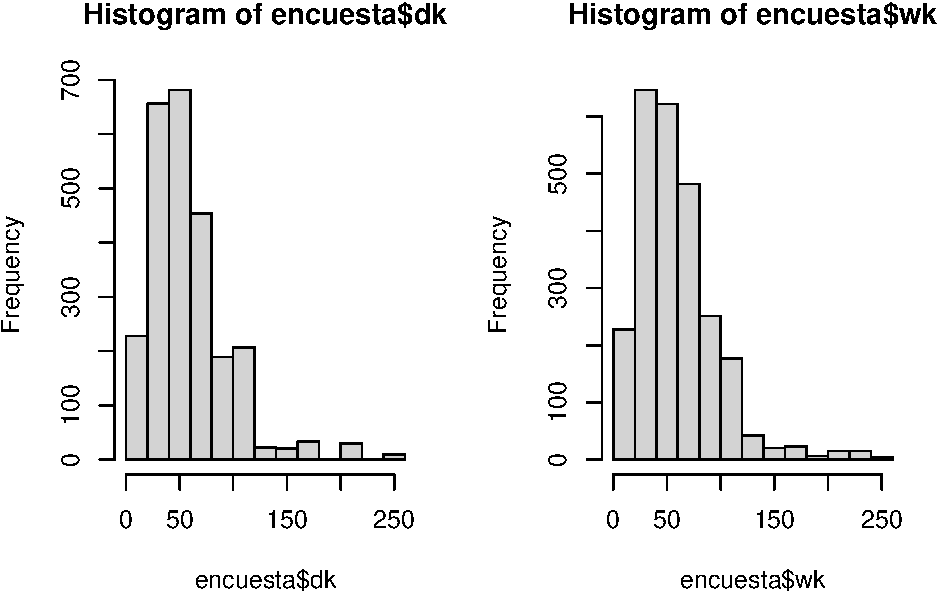
\includegraphics[width=0.9\linewidth]{02-Conceptos_files/figure-latex/unnamed-chunk-20-1} \end{center}

\begin{Shaded}
\begin{Highlighting}[]
\FunctionTok{plot}\NormalTok{(encuesta}\SpecialCharTok{$}\NormalTok{dk,encuesta}\SpecialCharTok{$}\NormalTok{wk)}
\end{Highlighting}
\end{Shaded}

\includegraphics{02-Conceptos_files/figure-latex/unnamed-chunk-21-1.pdf}

\begin{Shaded}
\begin{Highlighting}[]
\NormalTok{Region }\OtherTok{\textless{}{-}} \FunctionTok{as.numeric}\NormalTok{(}
  \FunctionTok{gsub}\NormalTok{(}\AttributeTok{pattern =} \StringTok{"}\SpecialCharTok{\textbackslash{}\textbackslash{}}\StringTok{D"}\NormalTok{,}
      \AttributeTok{replacement =}  \StringTok{""}\NormalTok{, }\AttributeTok{x =}\NormalTok{ encuesta}\SpecialCharTok{$}\NormalTok{Stratum))}
\NormalTok{encuesta}\SpecialCharTok{$}\NormalTok{Region }\OtherTok{\textless{}{-}} 
  \FunctionTok{cut}\NormalTok{(Region, }\AttributeTok{breaks =} \DecValTok{5}\NormalTok{,}
      \AttributeTok{labels =} \FunctionTok{c}\NormalTok{(}\StringTok{"Norte"}\NormalTok{,}\StringTok{"Sur"}\NormalTok{,}\StringTok{"Centro"}\NormalTok{,}\StringTok{"Occidente"}\NormalTok{,}\StringTok{"Oriente"}\NormalTok{))}
\NormalTok{encuesta }\SpecialCharTok{\%\textless{}\textgreater{}\%} \FunctionTok{mutate}\NormalTok{(}
  \AttributeTok{CatAge =} \FunctionTok{case\_when}\NormalTok{(}
\NormalTok{    Age }\SpecialCharTok{\textless{}=} \DecValTok{5} \SpecialCharTok{\textasciitilde{}} \StringTok{"0{-}5"}\NormalTok{,}
\NormalTok{    Age }\SpecialCharTok{\textless{}=} \DecValTok{15} \SpecialCharTok{\textasciitilde{}} \StringTok{"6{-}15"}\NormalTok{,}
\NormalTok{    Age }\SpecialCharTok{\textless{}=} \DecValTok{30} \SpecialCharTok{\textasciitilde{}} \StringTok{"16{-}30"}\NormalTok{,}
\NormalTok{    Age }\SpecialCharTok{\textless{}=} \DecValTok{45} \SpecialCharTok{\textasciitilde{}} \StringTok{"31{-}45"}\NormalTok{,}
\NormalTok{    Age }\SpecialCharTok{\textless{}=} \DecValTok{60} \SpecialCharTok{\textasciitilde{}} \StringTok{"46{-}60"}\NormalTok{,}
    \ConstantTok{TRUE} \SpecialCharTok{\textasciitilde{}} \StringTok{"Más de 60"}
\NormalTok{  ),}
  \AttributeTok{CatAge =} \FunctionTok{factor}\NormalTok{(}
\NormalTok{    CatAge,}
    \AttributeTok{levels =} \FunctionTok{c}\NormalTok{(}\StringTok{"0{-}5"}\NormalTok{, }\StringTok{"6{-}15"}\NormalTok{, }\StringTok{"16{-}30"}\NormalTok{, }\StringTok{"31{-}45"}\NormalTok{,}
               \StringTok{"46{-}60"}\NormalTok{, }\StringTok{"Más de 60"}\NormalTok{),}
    \AttributeTok{ordered =} \ConstantTok{TRUE}
\NormalTok{  )}
\NormalTok{)}
\FunctionTok{saveRDS}\NormalTok{(}\AttributeTok{object =}\NormalTok{ encuesta, }\AttributeTok{file =} \StringTok{"../Curso Tellez/Data/encuesta.rds"}\NormalTok{)}
\end{Highlighting}
\end{Shaded}

\hypertarget{manejando-una-base-de-encuestas-de-hogares-con-r}{%
\chapter{Manejando una base de encuestas de hogares con R}\label{manejando-una-base-de-encuestas-de-hogares-con-r}}

\hypertarget{fundamentos-buxe1sicos-de-r-y-rstudio}{%
\section{Fundamentos básicos de R y Rstudio}\label{fundamentos-buxe1sicos-de-r-y-rstudio}}

R fue creado en 1992 en Nueva Zelanda por Ross Ihaka y Robert Gentleman. A manera introductoria, R es un software diseñado para realizar análisis estadístico tanto sencillos como complejos. Este software a ganado popularidad en el gremio estadístico y no estadístico puesto que su manejo es sencillo y además, es de libre uso (Puede descargarse en \url{https://www.r-project.org}). Es decir, no requiere de ninguna licencia para su utilización. Como lo menciona Santana Sepúlveda, S., \& Mateos Farfán, E. (2014) R es un lenguaje de programación de libre distribución, bajo Licencia GNU, y se mantiene en un ambiente para el cómputo estadístico y gráfico. Este software está diseñado para utilizarse en distintos ambientes como, Windows, MacOS o Linux. El concepto de \emph{ambiente} está enfocado en caracterizarlo como un sistema totalmente planificado y coherente, en lugar de una acumulación gradual de herramientas muy específicas y poco flexibles, como suele ser con otro software de análisis de datos.

Ahora bien, como se mencionó anteriormente, R es un lenguaje de programación por ende, su interfase es poco amigable para los que inician en este lenguaje. Por esto, se creó RStudio el cual es un Entorno de Desarrollo Integrado (IDE, por sus siglas en inglés), lo que significa que RStudio es un programa que permite manejar R y utilizarlo de manera más cómoda y agradable.

\hypertarget{algunas-libreruxedas-de-interuxe9s}{%
\section{Algunas librerías de interés}\label{algunas-libreruxedas-de-interuxe9s}}

Puesto que \texttt{R} es un lenguaje colaborativo el cual permite que la comunidad vaya haciendo aportes al desarrollo de funciones dentro de paquetes o librerías. Alguna de las librerías más usadas para el análisis de bases de datos son las siguientes:

\begin{itemize}
\item
  \texttt{dplyr}, dplyr es la evolución del paquete plyr, enfocada en herramientas para trabajar con marcos de datos (de ahí la d en el nombre). Según Hadley Wickham, las siguientes son las tres propiedades principales de la librería:

  \begin{enumerate}
  \def\labelenumi{\arabic{enumi})}
  \item
    Identificar las herramientas de manipulación de datos más importantes necesarias para el análisis de datos y hacerlas fáciles de usar desde R.
  \item
    Proporcionar un rendimiento ultrarrápido para los datos en memoria escribiendo piezas clave en C++.
  \item
    Utilizar la misma interfaz para trabajar con datos sin importar dónde estén almacenados, ya sea en un marco de datos, una tabla de datos o una base de datos.Esta librería permite manejar eficientemente las bases de datos.
  \end{enumerate}
\item
  \texttt{tidyverse}, es una colección de paquetes disponibles en R y orientados a la manipulación, importación, exploración y visualización de datos y que se utiliza exhaustivamente en ciencia de datos. El uso de \texttt{tidyverse} permite facilitar el trabajo estadístico y la generación de trabajos reproducibles. Está compuesto de los siguientes paquetes: \texttt{readr}, \texttt{dplyr}, \texttt{ggplot2}, \texttt{tibble}, \texttt{tidyr}, \texttt{purr}, \texttt{stringr}, \texttt{forcats}
\item
  \texttt{readstata13}, este paquete permite leer y escribir todos los formatos de archivo de Stata (versión 17 y anteriores) en un marco de datos R. Se admiten las versiones de formato de archivo de datos 102 a 119. para leer las bases de datos de \texttt{STATA}. Además, el paquete admite muchas características del formato Stata dta, como conjuntos de etiquetas en diferentes idiomas o calendarios comerciales.
\item
  \texttt{survey}, este paquete ha sido elaborado por el Profesor Thomas Lumley (Lumley, T. 2011) y nos proporciona funciones en R útiles para analizar datos provenientes de encuestas complejas.Alguno de los parámetros que se pueden estimar usando este paquete son medias, totales, razones, cuantiles, tablas de contingencias, modelos de regresión, modelos loglineales, entre otros.
\item
  \texttt{srvyr}, este paquete permite utilizar el operador \emph{pipe operators} en las consultas que se realizan con el paquete \texttt{survey}.
\item
  \texttt{ggplot2}, es un paquete de visualización de datos para el lenguaje R que implementa lo que se conoce como la \emph{Gramática de los Gráficos}, que no es más que una representación esquemática y en capas de lo que se dibuja en dichos gráficos, como lo pueden ser los marcos y los ejes, el texto de los mismos, los títulos, así como, por supuesto, los datos o la información que se grafica, el tipo de gráfico que se utiliza, los colores, los símbolos y tamaños, entre otros.
\item
  \texttt{TeachingSampling}, este paquete permite al usuario extraer muestras probabilísticas y hacer inferencias a partir de una población finita basada en varios diseños de muestreo. Entre los diseño empleados en esta librería están: Muestreo Aleatorio Simple (MAS), Muestreo Bernoullí, Muestreo Sistemático, PiPT, PPT, estre otros.
\item
  \texttt{samplesize4surveys}, este paquete permite calcular el tamaño de muestra requerido para la estimación de totales, medias y proporciones bajo diseños de muestreo complejos.
\end{itemize}

Antes de poder utilizar las diferentes funciones que cada librería tiene, es necesario descargarlas de antemano de la web. El comando \texttt{install.packages} permite realizar esta tarea. Note que algunas librerías pueden depender de otras, así que para poder utilizarlas es necesario instalar también las dependencias.

\begin{Shaded}
\begin{Highlighting}[]
\FunctionTok{install.packages}\NormalTok{(}\StringTok{"dplyr"}\NormalTok{)}
\FunctionTok{install.packages}\NormalTok{(}\StringTok{"tidyverse"}\NormalTok{)}
\FunctionTok{install.packages}\NormalTok{(}\StringTok{"readstata13"}\NormalTok{) }
\FunctionTok{install.packages}\NormalTok{(}\StringTok{"survey"}\NormalTok{)}
\FunctionTok{install.packages}\NormalTok{(}\StringTok{"srvyr"}\NormalTok{)}
\FunctionTok{install.packages}\NormalTok{(}\StringTok{"ggplot2"}\NormalTok{)}
\FunctionTok{install.packages}\NormalTok{(}\StringTok{"TeachingSampling"}\NormalTok{)}
\FunctionTok{install.packages}\NormalTok{(}\StringTok{"samplesize4surveys"}\NormalTok{)}
\end{Highlighting}
\end{Shaded}

Una vez instaladas las librerías hay que informarle al software que vamos a utilizarlas con el comando \texttt{library}. \emph{Recuerde que es necesario haber instalado las librerías para poder utilizarlas}.

\begin{Shaded}
\begin{Highlighting}[]
\FunctionTok{rm}\NormalTok{(}\AttributeTok{list =} \FunctionTok{ls}\NormalTok{())}

\FunctionTok{library}\NormalTok{(}\StringTok{"dplyr"}\NormalTok{)}
\FunctionTok{library}\NormalTok{(}\StringTok{"tidyverse"}\NormalTok{)}
\FunctionTok{library}\NormalTok{(}\StringTok{"readstata13"}\NormalTok{) }
\FunctionTok{library}\NormalTok{(}\StringTok{"survey"}\NormalTok{)}
\FunctionTok{library}\NormalTok{(}\StringTok{"srvyr"}\NormalTok{)}
\FunctionTok{library}\NormalTok{(}\StringTok{"ggplot2"}\NormalTok{)}
\FunctionTok{library}\NormalTok{(}\StringTok{"TeachingSampling"}\NormalTok{)}
\FunctionTok{library}\NormalTok{(}\StringTok{"samplesize4surveys"}\NormalTok{)}
\end{Highlighting}
\end{Shaded}

\hypertarget{craciuxf3n-de-proyectos-en-r}{%
\section{\texorpdfstring{Cración de proyectos en \texttt{R}}{Cración de proyectos en R}}\label{craciuxf3n-de-proyectos-en-r}}

Una vez se descargan e instalan las librerías o paquetes en \texttt{R} el paso siguientes es crear proyectos. Un proyecto de R se define como un archivo que contiene los archivos de origen y contenido asociados con el trabajo que se está realizando. Adicionalmente, contiene información que permite la compilación de cada archivo de R a utilizar, mantiene la información para integrarse con sistemas de control de código fuente y ayuda a organizar la aplicación en componentes lógicos.

Ahora bien, por una cultura de buenas practicas de programación, se recomienda crear un proyecto en el cual se tenga disponible toda la información a trabajar. A continuación, se muestran los pasos para crear un proyecto dentro de \texttt{RStrudio}.

\begin{itemize}
\item
  \textbf{Paso 1:} Abrir \texttt{RStudio}.
\item
  \textbf{Paso 2:} ir a file -\textgreater{} New Project 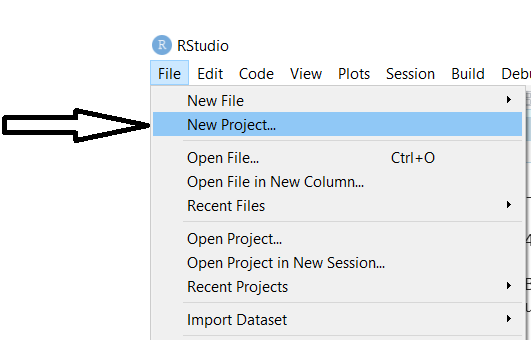
\includegraphics[width=4.6875in,height=\textheight]{Imagenes/Cap 0/Proyecto1.png}
\item
  \emph{Paso 3:} Tipos de proyecto.
\end{itemize}

Para este ejemplo se tomará \emph{New Directory}

\begin{figure}
\centering
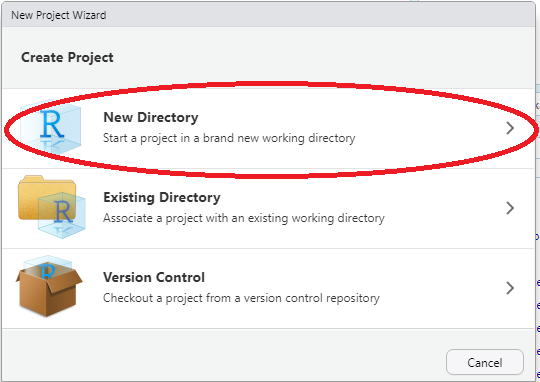
\includegraphics[width=4.6875in,height=\textheight]{Imagenes/Cap 0/Proyecto2.png}
\caption{\emph{Tipos de proyectos}}
\end{figure}

Algo a tener en cuenta en este paso es que en \emph{New Directory} \texttt{RStudio} brinda una variedad de opciones dependiendo las características del procesamiento que desea realizar. Ahora bien, si se cuenta con algunos código previamente desarrollados y se desea continuar con ese proyecto, se debe tomar la opción \emph{Existing Directory} . Por último, Si se cuenta con cuenta en \emph{Git} y se desea tener una copia de seguridad, se debe emplear la opción \emph{Version Control}.

\begin{itemize}
\tightlist
\item
  \emph{Paso 4:} Seleccionar el tipo de proyecto.
\end{itemize}

\begin{figure}
\centering
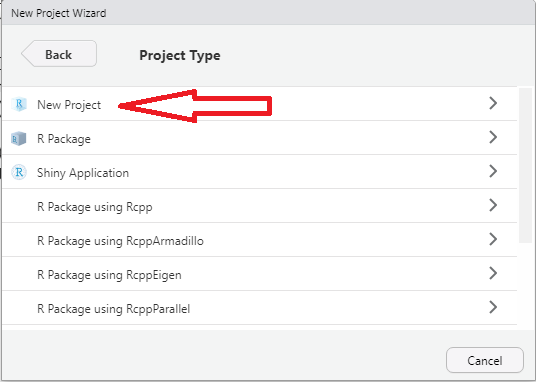
\includegraphics[width=4.6875in,height=\textheight]{Imagenes/Cap 0/Proyecto3.png}
\caption{\emph{Seleccionar el tipo de proyecto}}
\end{figure}

\begin{itemize}
\tightlist
\item
  \emph{Paso 5}: Diligenciar el nombre del proyecto y la carpeta de destino.
\end{itemize}

\begin{figure}
\centering
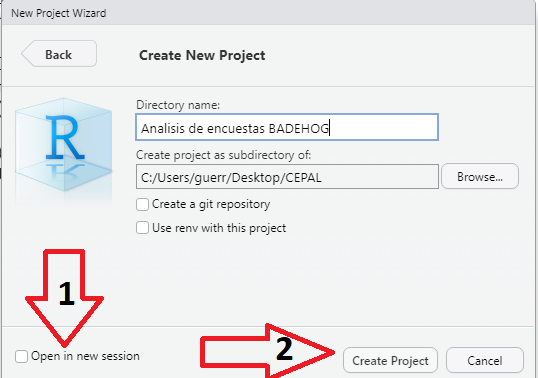
\includegraphics[width=4.6875in,height=\textheight]{Imagenes/Cap 0/Proyecto4.png}
\caption{\emph{Nombre de proyecto}}
\end{figure}

Al realizar esto pasos permite que todas rutinas creadas dentro del proyecto estén ancladas a la carpeta del proyecto.

\hypertarget{lectura-de-las-bases-de-datos-y-manipulaciuxf3n}{%
\section{Lectura de las bases de datos y manipulación}\label{lectura-de-las-bases-de-datos-y-manipulaciuxf3n}}

Es muy usual que al trabajar proyectos en \texttt{R} sea necesario importar bases de datos con información relevante para un estudio en particular. En Colombia, por ejemplo, en la \emph{Encuesta de Calidad de Vida (ECV, por sus siglas)} es necesario, una vez se realiza el trabajo de campo, importar la información recolectada para poder ajustar los factores de expansión y posteriormente estimar los parámetros. Los formatos de bases de datos que \texttt{R} permite importar son diversos, entre ellos se tienen \texttt{xlsx}, \texttt{csv}, \texttt{txt}, \texttt{STATA}, etc. Particularmente, para la lectura de bases de datos provenientes de \texttt{STATA\ 13} se realiza con la función \texttt{read.dta13}. Una vez leída la base de datos en el formato mencionado anteriormente se procede a transformar en el formato \texttt{.RDS} el cual es un formato más eficiente y propio de \texttt{R}. Para ejemplificar los procedimientos en \texttt{R} se utilizará la base de datos de \emph{Pesquisa Nacional por Amostra de Domicílios 2015 } de Brasil la cual está en formato \texttt{.dta} el cual se lee en \texttt{R} con la función \texttt{read.dta13}. Posteriormente se transformará al formato \texttt{.rds} con la función \texttt{saveRDS} el cual es un formato propio de \texttt{R} y por último se cargar esta base. Lo pasos anteriores se realiza como sigue:

Primero se carga la base en formato \texttt{dta} con la librería \texttt{read.dta13} y se guarda en formato \texttt{rds} con la función \texttt{saveRDS}
`

\begin{Shaded}
\begin{Highlighting}[]
\NormalTok{data1 }\OtherTok{\textless{}{-}} \FunctionTok{read.dta13}\NormalTok{(}\StringTok{"Z:/BC/BRA\_2015N.dta"}\NormalTok{)}
\FunctionTok{saveRDS}\NormalTok{(data1, }\StringTok{"../data/BRA\_2015N.rds"}\NormalTok{) }
\end{Highlighting}
\end{Shaded}

Una vez guardada la base en nuestros archivos de trabajo, se procede a cargar la base a \texttt{R} con la función \texttt{readRDS} para poder utilizar toda la información que en ella se contiene.

\begin{Shaded}
\begin{Highlighting}[]
\NormalTok{data2 }\OtherTok{\textless{}{-}} \FunctionTok{readRDS}\NormalTok{(}\StringTok{"Data/BRA\_2015N.rds"}\NormalTok{)}
\end{Highlighting}
\end{Shaded}

Una vez cargada la base de datos en \texttt{R} ésta se puede empezar a manipular según las necesidades de cada investigador. En este sentido, una de las primeras revisiones que se realizan al cargar las bases de datos es revisar su dimensión, es decir, chequear la cantidad de filas y columnas que tenga la base. Lo anterior se puede hacer con la función \texttt{nrow}. Dicha función identifica el número de registros (unidades efectivamente medidas) en la base de datos y la función \texttt{ncol} muestra el número de variables en la base de datos. Los códigos computacionales son los siguientes:

\begin{Shaded}
\begin{Highlighting}[]
\FunctionTok{nrow}\NormalTok{(data2)}
\end{Highlighting}
\end{Shaded}

\begin{verbatim}
## [1] 356904
\end{verbatim}

\begin{Shaded}
\begin{Highlighting}[]
\FunctionTok{ncol}\NormalTok{(data2)}
\end{Highlighting}
\end{Shaded}

\begin{verbatim}
## [1] 109
\end{verbatim}

Una forma resumida de revisar la cantidad de filas y columnas que tiene la base de datos es usar la función \texttt{dim}. Esta función nos devuelve un vector indicado en su primera componente la cantidad de fila y en su segundo la cantidad de columnas como se muestra a continuación:

\begin{Shaded}
\begin{Highlighting}[]
\FunctionTok{dim}\NormalTok{(data2)}
\end{Highlighting}
\end{Shaded}

\begin{verbatim}
## [1] 356904    109
\end{verbatim}

Es usual que en las encuestas de hogares las bases de datos sean muy extensas, es decir, contengan una cantidad importante de variables medidas (filas) y por lo general, el tamaño de la muestra de estos estudios con grandes. Es por lo anterior que, para poder visualizar dichas bases una vez cargadas en \texttt{R}, es necesario hacerlo de manera externa. Esto es, abrir una pestaña diferente en \texttt{R} y hacer la navegación de la base como un texto plano. Lo anterior se realiza con la función \texttt{View} como se muestra a continuación:

\begin{Shaded}
\begin{Highlighting}[]
\FunctionTok{View}\NormalTok{(data2)}
\end{Highlighting}
\end{Shaded}

\begin{figure}
\centering
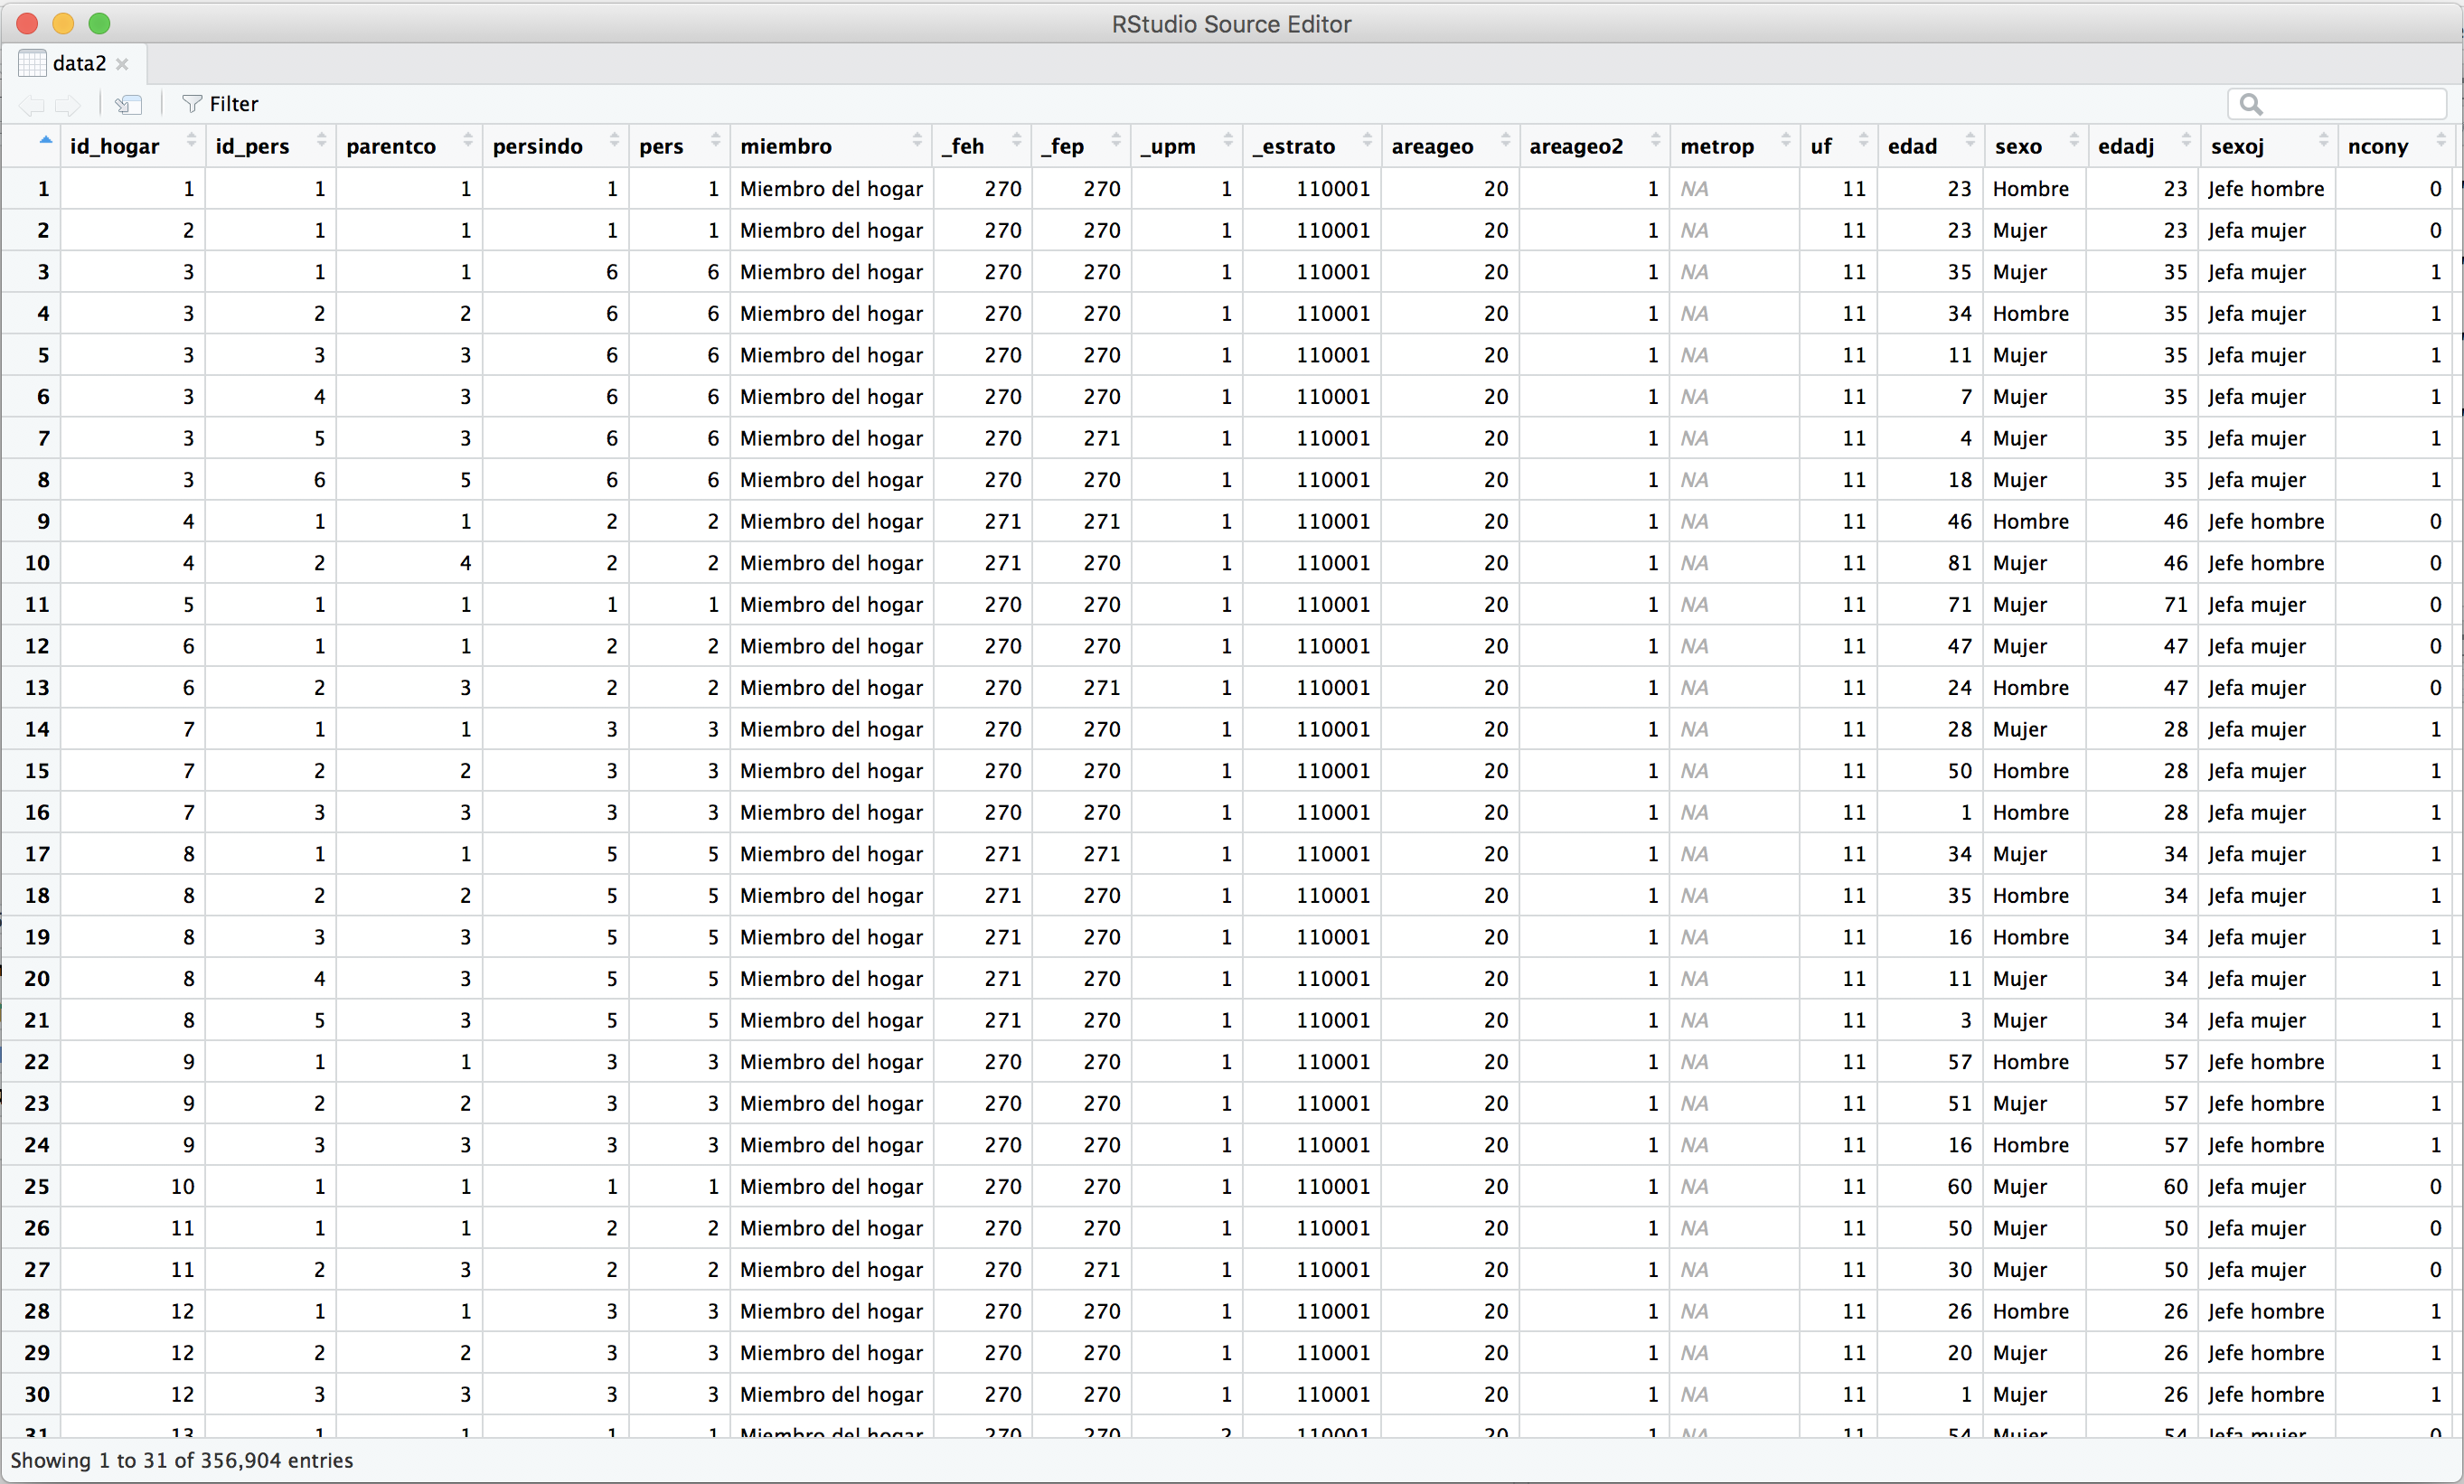
\includegraphics[width=8.85417in,height=\textheight]{Imagenes/Cap 0/1.png}
\caption{\emph{Visor de bases de datos de RStudio}}
\end{figure}

Otro chequeo importante que se debe realizar al momento de cargar una base de datos en \texttt{R} es el reconocimiento de las variables que incluye. Esto se puede hacer utilizando la función \texttt{names} la cual identifica las variables de la base de datos.

\begin{Shaded}
\begin{Highlighting}[]
\FunctionTok{names}\NormalTok{(data2)}
\end{Highlighting}
\end{Shaded}

La función \texttt{names} solo devuelve un vector un vector con los nombres de las variables que contiene la base. Sin embargo, si se quiere profundizar en qué información contiene cada variable, La función \texttt{str} muestra de manera compacta la estructura de un objeto y sus componentes. Para nuestra base se utilizaría de la siguiente manera:

\begin{Shaded}
\begin{Highlighting}[]
\FunctionTok{str}\NormalTok{(data2)}
\end{Highlighting}
\end{Shaded}

Como se puede observar en la salida anterior, por ejemplo, la variable \emph{id\_hogar} es de tipo \emph{Entero} al igual que \emph{id\_pers} mientras que \emph{cotiza\_ee} es un factor con 2 niveles. Como se observa, esta función es muy útil al momento de querer tener un panorama amplio del contenido y clase de cada variable en una base de datos, particularmente, en una encuesta de hogares en donde se tiene, por la misma estructura del estudio, muchas clases o tipos de variables medidas.

\hypertarget{el-operador-pipe}{%
\section{\texorpdfstring{El operador \texttt{pipe}}{El operador pipe}}\label{el-operador-pipe}}

El software estadístico \texttt{R} es un lenguaje de programación creado por estadísticos para estadísticos. Una de las contribuciones recientes es el desarrollo de los \texttt{pipelines} que permiten de una forma intuitiva generar consultas y objetos desde una base de datos. El operador \emph{pipe}, \texttt{\%\textgreater{}\%}, viene del paquete magrittr (Bache, S. et al., 2022) y está cargado automáticamente en los paquetes del \texttt{Tidyverse}.

El objetivo del operador pipe es ayudar a escribir código de una manera que sea más fácil de leer y entender. En este sentido, el operador \texttt{\%\textgreater{}\%} permite ``encadenar'' operaciones en el sentido que el resultado de una operación anterior se convierta en el input de la siguiente operación. A continuación, ejemplificaremos el uso del \texttt{\%\textgreater{}\%} en la base de datos de Brasil haciendo un conteo del total de elementos que contiene la base de datos utilizando la función \texttt{count}.

\begin{Shaded}
\begin{Highlighting}[]
\NormalTok{data2 }\SpecialCharTok{\%\textgreater{}\%} \FunctionTok{count}\NormalTok{()}
\end{Highlighting}
\end{Shaded}

\begin{verbatim}
##        n
## 1 356904
\end{verbatim}

Otra operación que se puede realizar en \texttt{R} es re-codificar los niveles de los factores que en muchas ocasiones son necesarios en las encuestas de hogares. El siguiente código permite generar los nombres de los estados en Brasil.

\begin{Shaded}
\begin{Highlighting}[]
\NormalTok{data2}\SpecialCharTok{$}\NormalTok{estados }\OtherTok{\textless{}{-}} \FunctionTok{factor}\NormalTok{(data2}\SpecialCharTok{$}\NormalTok{uf, }
 \AttributeTok{levels =} \FunctionTok{c}\NormalTok{(}\DecValTok{11}\SpecialCharTok{:}\DecValTok{17}\NormalTok{, }\DecValTok{21}\SpecialCharTok{:}\DecValTok{29}\NormalTok{, }\DecValTok{31}\SpecialCharTok{:}\DecValTok{33}\NormalTok{, }\DecValTok{35}\NormalTok{, }\DecValTok{41}\SpecialCharTok{:}\DecValTok{43}\NormalTok{, }\DecValTok{50}\SpecialCharTok{:}\DecValTok{53}\NormalTok{), }
 \AttributeTok{labels =} \FunctionTok{c}\NormalTok{(}\StringTok{"Rondonia"}\NormalTok{, }\StringTok{"Acre"}\NormalTok{, }\StringTok{"Amazonas"}\NormalTok{, }\StringTok{"Roraima"}\NormalTok{, }
            \StringTok{"Para"}\NormalTok{, }\StringTok{"Amapa"}\NormalTok{, }\StringTok{"Tocantins"}\NormalTok{, }\StringTok{"Maranhao"}\NormalTok{, }
            \StringTok{"Piaui"}\NormalTok{, }\StringTok{"Ceara"}\NormalTok{, }\StringTok{"RioGrandeNorte"}\NormalTok{, }\StringTok{"Paraiba"}\NormalTok{,}
            \StringTok{"Pernambuco"}\NormalTok{, }\StringTok{"Alagoas"}\NormalTok{, }\StringTok{"Sergipe"}\NormalTok{, }\StringTok{"Bahia"}\NormalTok{, }
            \StringTok{"MinasGerais"}\NormalTok{, }\StringTok{"EspirituSanto"}\NormalTok{, }\StringTok{"RioJaneiro"}\NormalTok{, }
            \StringTok{"SaoPaulo"}\NormalTok{, }\StringTok{"Parana"}\NormalTok{, }\StringTok{"SantaCatarina"}\NormalTok{, }
            \StringTok{"RioGrandeSur"}\NormalTok{, }\StringTok{"MatoGrossoSur"}\NormalTok{, }\StringTok{"MatoGrosso"}\NormalTok{, }
            \StringTok{"Goias"}\NormalTok{, }\StringTok{"DistritoFederal"}\NormalTok{))}
\end{Highlighting}
\end{Shaded}

Adicionalmente, para efectos de visualización en tablas y gráficos es conviene codificar los nombres de las variables. Para este ejemplo, se codificarán de la siguiente manera:

\begin{Shaded}
\begin{Highlighting}[]
\NormalTok{data2}\SpecialCharTok{$}\NormalTok{deptos }\OtherTok{\textless{}{-}} \FunctionTok{factor}\NormalTok{(data2}\SpecialCharTok{$}\NormalTok{uf, }
 \AttributeTok{levels =} \FunctionTok{c}\NormalTok{(}\DecValTok{11}\SpecialCharTok{:}\DecValTok{17}\NormalTok{, }\DecValTok{21}\SpecialCharTok{:}\DecValTok{29}\NormalTok{, }\DecValTok{31}\SpecialCharTok{:}\DecValTok{33}\NormalTok{, }\DecValTok{35}\NormalTok{, }\DecValTok{41}\SpecialCharTok{:}\DecValTok{43}\NormalTok{, }\DecValTok{50}\SpecialCharTok{:}\DecValTok{53}\NormalTok{), }
 \AttributeTok{labels =} \FunctionTok{c}\NormalTok{(}\StringTok{"RO"}\NormalTok{, }\StringTok{"AC"}\NormalTok{, }\StringTok{"AM"}\NormalTok{, }\StringTok{"RR"}\NormalTok{, }\StringTok{"PA"}\NormalTok{, }
 \StringTok{"AP"}\NormalTok{, }\StringTok{"TO"}\NormalTok{, }\StringTok{"MA"}\NormalTok{, }\StringTok{"PI"}\NormalTok{, }\StringTok{"CE"}\NormalTok{, }\StringTok{"RN"}\NormalTok{, }\StringTok{"PB"}\NormalTok{, }
 \StringTok{"PE"}\NormalTok{, }\StringTok{"AL"}\NormalTok{, }\StringTok{"SE"}\NormalTok{, }\StringTok{"BA"}\NormalTok{, }\StringTok{"MG"}\NormalTok{, }\StringTok{"ES"}\NormalTok{, }\StringTok{"RJ"}\NormalTok{, }\StringTok{"SP"}\NormalTok{,}
 \StringTok{"PR"}\NormalTok{, }\StringTok{"SC"}\NormalTok{, }\StringTok{"RS"}\NormalTok{, }\StringTok{"MS"}\NormalTok{, }\StringTok{"MT"}\NormalTok{, }\StringTok{"GO"}\NormalTok{, }\StringTok{"DF"}\NormalTok{))}
\end{Highlighting}
\end{Shaded}

Por otro lado, existe una gama amplia de funciones que se pueden utilizar con el operador \texttt{\%\textgreater{}\%}, A continuación, se enlistan una serie de funciones muy útiles al momento de hacer análisis con bases de datos provenientes de encuestas de hogares:

\begin{itemize}
\tightlist
\item
  \textbf{filter}: mantiene un criterio de filtro sobre alguna variable o mezcla de variables.
\item
  \textbf{select}: selecciona columnas por nombres.
\item
  \textbf{arrange}: ordena las filas de la base de datos.
\item
  \textbf{mutate}: añade nuevas variables a la base de datos.
\item
  \textbf{summarise}: reduce variables a valores y los presenta en una tabla.
\item
  \textbf{group\_by}: ejecuta funciones y agrupa el resultado por las variables de interés.
\end{itemize}

Ejemplificando alguna de las funciones mostradas anteriormente, una de las primeras consultas que se realizan en las encuestas de hogares es saber el número de encuestas (personas) realizadas y que están contenida en la base de datos. Usando \texttt{\%\textgreater{}\%} se realiza de la siguiente manera:

\begin{Shaded}
\begin{Highlighting}[]
\NormalTok{data2 }\SpecialCharTok{\%\textgreater{}\%} \FunctionTok{count}\NormalTok{()}
\end{Highlighting}
\end{Shaded}

\begin{verbatim}
##        n
## 1 356904
\end{verbatim}

Otro de los ejercicios que se hacen usualmente con las encuestas de hogares está relacionado con saber la cantidad de hogares que hay en el país de estudio. Una de las formas más sencillas de hacer esta revisión es usar la función \texttt{filter}. Las encuestas de hogares muchas veces recopilan información a nivel de viviendas, hogares y personas. Particularmente, las bases de datos que están disponibles en \texttt{BADEHOG} están a nivel de persona. Ahora bien, para saber la cantidad de hogares que se encuestaron basta con filtrar por hogar porque sólo hay un jefe de hogar por hogar, como se muestra a continuación:

\begin{Shaded}
\begin{Highlighting}[]
\NormalTok{datahogar1 }\OtherTok{\textless{}{-}}\NormalTok{ data2 }\SpecialCharTok{\%\textgreater{}\%} \FunctionTok{filter}\NormalTok{(parentco }\SpecialCharTok{==} \DecValTok{1}\NormalTok{)}
\NormalTok{datahogar2 }\OtherTok{\textless{}{-}}\NormalTok{ data2 }\SpecialCharTok{\%\textgreater{}\%} \FunctionTok{filter}\NormalTok{(paren\_ee }\SpecialCharTok{==} \StringTok{"Jefe"}\NormalTok{) }
\end{Highlighting}
\end{Shaded}

Por otro lado, si el interés ahora es filtrar la base de datos por la ubicación de la persona en el área rural y urbana se realiza de la siguiente manera:

\begin{Shaded}
\begin{Highlighting}[]
\NormalTok{dataurbano }\OtherTok{\textless{}{-}}\NormalTok{ data2 }\SpecialCharTok{\%\textgreater{}\%} 
  \FunctionTok{filter}\NormalTok{(area\_ee }\SpecialCharTok{==} \StringTok{"Area urbana"}\NormalTok{)}
\NormalTok{datarural }\OtherTok{\textless{}{-}}\NormalTok{ data2 }\SpecialCharTok{\%\textgreater{}\%} 
  \FunctionTok{filter}\NormalTok{(area\_ee }\SpecialCharTok{==} \StringTok{"Area rural"}\NormalTok{) }
\end{Highlighting}
\end{Shaded}

En este mismo sentido, si el objetivo ahora es filtrar la base de datos por algunos ingresos particulares mensuales por personas, por ejemplo, altos o bajos, se realiza de la siguiente manera:

\begin{Shaded}
\begin{Highlighting}[]
\NormalTok{dataingreso1 }\OtherTok{\textless{}{-}}\NormalTok{ data2 }\SpecialCharTok{\%\textgreater{}\%} 
  \FunctionTok{filter}\NormalTok{(ingcorte }\SpecialCharTok{\%in\%} \FunctionTok{c}\NormalTok{(}\DecValTok{50}\NormalTok{, }\DecValTok{100}\NormalTok{))}

\NormalTok{dataingreso2 }\OtherTok{\textless{}{-}}\NormalTok{ data2 }\SpecialCharTok{\%\textgreater{}\%} 
  \FunctionTok{filter}\NormalTok{(ingcorte }\SpecialCharTok{\%in\%} \FunctionTok{c}\NormalTok{(}\DecValTok{1000}\NormalTok{, }\DecValTok{2000}\NormalTok{))}
\end{Highlighting}
\end{Shaded}

Otra función muy útil en el análisis en encuestas de hogares es la función \texttt{select} la cual, como se mencionó anteriormente permite seleccionar un grupo de variables de interés a analizar. Si por ejemplo, se desea seleccionar de la base de ejemplo solo las variables identificación del hogar (\texttt{id\_hogar}), unidades primarias de muestreo (\texttt{\_upm}), factores de expansión (\texttt{\_feh}) y estratos muestrales ( \texttt{\_estrato}) se realiza de la siguiente manera:

\begin{Shaded}
\begin{Highlighting}[]
\NormalTok{datared }\OtherTok{\textless{}{-}}\NormalTok{ data2 }\SpecialCharTok{\%\textgreater{}\%} \FunctionTok{select}\NormalTok{(}\StringTok{\textasciigrave{}}\AttributeTok{id\_hogar}\StringTok{\textasciigrave{}}\NormalTok{, }\StringTok{\textasciigrave{}}\AttributeTok{\_upm}\StringTok{\textasciigrave{}}\NormalTok{,}
                            \StringTok{\textasciigrave{}}\AttributeTok{\_feh}\StringTok{\textasciigrave{}}\NormalTok{, }\StringTok{\textasciigrave{}}\AttributeTok{\_estrato}\StringTok{\textasciigrave{}}\NormalTok{)}

\NormalTok{datablue }\OtherTok{\textless{}{-}}\NormalTok{ data2 }\SpecialCharTok{\%\textgreater{}\%} \FunctionTok{select}\NormalTok{(id\_pers, edad, }
\NormalTok{                             sexo, ingcorte)}
\end{Highlighting}
\end{Shaded}

La función \texttt{select} no solo sirve para seleccionar variables de una base de datos, también se puede utilizar para eliminar algunas variables de la base de datos que ya no son de interés para el análisis o que simplemente se generaron en la manipulación de la base de datos como variables puentes para realizar algunos cálculos de interés. Por ejemplo, si se desea eliminar de la base de datos de ejemplo las variables identificación del hogar (\texttt{id\_hogar}) e identificación de las personas (\texttt{id\_pers}) se realiza introduciendo un signo ``menos'' (-) delante del nombre de la variable como sigue:

\begin{Shaded}
\begin{Highlighting}[]
\NormalTok{datagrey }\OtherTok{\textless{}{-}}\NormalTok{ data2 }\SpecialCharTok{\%\textgreater{}\%} \FunctionTok{select}\NormalTok{(}\SpecialCharTok{{-}}\NormalTok{id\_hogar, }\SpecialCharTok{{-}}\NormalTok{id\_pers)}
\end{Highlighting}
\end{Shaded}

Por otro lado, si el objetivo ahora en análisis de las encuestas de hogares es ordenar las filas de la base por alguna variable en particular, se utiliza en \texttt{R} la función \texttt{arrange} para realizar esta operación. A continuación, se ejemplifica con la base de datos de ejemplo, cómo se ordena la base de acuerdo con la variable \emph{ingcorte}:

\begin{Shaded}
\begin{Highlighting}[]
\NormalTok{datadog }\OtherTok{\textless{}{-}}\NormalTok{ datablue }\SpecialCharTok{\%\textgreater{}\%} \FunctionTok{arrange}\NormalTok{(ingcorte)}
\NormalTok{datadog }\SpecialCharTok{\%\textgreater{}\%} \FunctionTok{head}\NormalTok{()}
\end{Highlighting}
\end{Shaded}

\begin{verbatim}
##   id_pers edad   sexo ingcorte
## 1       1   38  Mujer        0
## 2       2   12  Mujer        0
## 3       1   26 Hombre        0
## 4       2   29  Mujer        0
## 5       1   50 Hombre        0
## 6       1   53  Mujer        0
\end{verbatim}

Es posible utilizar la función \texttt{arrange} para hacer ordenamientos más complicados. Por ejemplo, ordenar por más de una variable. A modo de ejemplo, ordenemos la base de datos \emph{datablue} de acuerdo con las variables \emph{sexo} y \emph{edad}

\begin{Shaded}
\begin{Highlighting}[]
\NormalTok{datablue }\SpecialCharTok{\%\textgreater{}\%} \FunctionTok{arrange}\NormalTok{(sexo, edad) }\SpecialCharTok{\%\textgreater{}\%} \FunctionTok{head}\NormalTok{()}
\end{Highlighting}
\end{Shaded}

\begin{verbatim}
##   id_pers edad   sexo  ingcorte
## 1       6    0 Hombre  660.4400
## 2       6    0 Hombre  162.5000
## 3       3    0 Hombre  381.6667
## 4       5    0 Hombre  320.0000
## 5       6    0 Hombre  375.0000
## 6       4    0 Hombre 1425.0000
\end{verbatim}

También es posible utilizar la función \texttt{arrange} junto con la opción \texttt{desc()} para que el ordenamiento sea descendente.

\begin{Shaded}
\begin{Highlighting}[]
\NormalTok{datablue }\SpecialCharTok{\%\textgreater{}\%} \FunctionTok{arrange}\NormalTok{(}\FunctionTok{desc}\NormalTok{(edad)) }\SpecialCharTok{\%\textgreater{}\%} \FunctionTok{head}\NormalTok{()}
\end{Highlighting}
\end{Shaded}

\begin{verbatim}
##   id_pers edad   sexo  ingcorte
## 1       2  115  Mujer  103.0000
## 2       4  110  Mujer 1156.5300
## 3       2  107 Hombre  415.5904
## 4       1  107  Mujer 1754.4600
## 5       3  105  Mujer  380.7904
## 6       2  105  Mujer  898.3200
\end{verbatim}

\hypertarget{funciones-mutate-summarise-y-group_by-en-encuestas-de-hogares}{%
\section{\texorpdfstring{Funciones \textbf{mutate, summarise y group\_by} en encuestas de hogares}{Funciones mutate, summarise y group\_by en encuestas de hogares}}\label{funciones-mutate-summarise-y-group_by-en-encuestas-de-hogares}}

Las funciones \texttt{mutate}, \texttt{summarise} y \texttt{group\_by} están cargadas en el paquete \texttt{tidyverse} y son muy importantes al momento de realizar análisis en encuestas de hogares. En primer lugar, la función \texttt{mutate} permite computar transformaciones de variables en una base de datos. Usualmente, en las encuestas de hogares es necesario crear nuevas variables, por ejemplo, si el hogar está en estado de pobreza extrema o no la cual se calcula a partir de los ingresos del hogar, la función \texttt{mutate} proporciona una interface clara para realizar este tipo de operaciones. A modo de ejemplo, utilizaremos la base de ejemplo para crear una nueva variable llamada \emph{ingreso2} la cual es el doble de los ingresos por persona dentro de un hogar. Los códigos computacionales se muestran a continuación:

\begin{Shaded}
\begin{Highlighting}[]
\NormalTok{datablue2 }\OtherTok{\textless{}{-}}\NormalTok{ datablue }\SpecialCharTok{\%\textgreater{}\%} 
  \FunctionTok{mutate}\NormalTok{(}\AttributeTok{ingreso2 =} \DecValTok{2} \SpecialCharTok{*}\NormalTok{ ingcorte)}
\NormalTok{datablue2 }\SpecialCharTok{\%\textgreater{}\%} \FunctionTok{head}\NormalTok{()}
\end{Highlighting}
\end{Shaded}

\begin{verbatim}
##   id_pers edad   sexo ingcorte ingreso2
## 1       1   23 Hombre    800.0   1600.0
## 2       1   23  Mujer   1150.0   2300.0
## 3       1   35  Mujer    904.4   1808.8
## 4       2   34 Hombre    904.4   1808.8
## 5       3   11  Mujer    904.4   1808.8
## 6       4    7  Mujer    904.4   1808.8
\end{verbatim}

No solo se puede crear una nueva variable, si es necesario, se pueden crear más de una variable en la base de datos. Cabe recalcar que la función \texttt{mutate} reconoce sistemáticamente las variables que van siendo creadas de manera ordenada. A continuación, se presenta cómo crear más de una nueva variable en la base de datos:

\begin{Shaded}
\begin{Highlighting}[]
\NormalTok{datacat }\OtherTok{\textless{}{-}}\NormalTok{ datablue }\SpecialCharTok{\%\textgreater{}\%} 
  \FunctionTok{mutate}\NormalTok{(}\AttributeTok{ingreso2 =} \DecValTok{2} \SpecialCharTok{*}\NormalTok{ ingcorte,}
         \AttributeTok{ingreso4 =} \DecValTok{2} \SpecialCharTok{*}\NormalTok{ ingreso2)}
\NormalTok{datacat }\SpecialCharTok{\%\textgreater{}\%} \FunctionTok{head}\NormalTok{()}
\end{Highlighting}
\end{Shaded}

\begin{verbatim}
##   id_pers edad   sexo ingcorte ingreso2 ingreso4
## 1       1   23 Hombre    800.0   1600.0   3200.0
## 2       1   23  Mujer   1150.0   2300.0   4600.0
## 3       1   35  Mujer    904.4   1808.8   3617.6
## 4       2   34 Hombre    904.4   1808.8   3617.6
## 5       3   11  Mujer    904.4   1808.8   3617.6
## 6       4    7  Mujer    904.4   1808.8   3617.6
\end{verbatim}

Ahora bien, la función \texttt{summarise} funciona de forma similar a la función \texttt{mutate}, excepto que en lugar de añadir nuevas columnas crea un nuevo data frame. Como se mencionó anteriormente esta función sirve para resumir o ``colapsar filas''. Toma un grupo de valores como input y devuelve un solo valor; por ejemplo, hallar la media de los ingresos, percentiles o medidas de dispersión.

Por otro lado, la función \texttt{group\_by} permite agrupar información de acuerdo con una(s) variable(s) de interés. El siguiente código permite generar el número de encuestas efectivas en cada uno de los estados de Brasil. El comando \texttt{group\_by} agrupa los datos por estados, el comando \texttt{summarise} hace los cálculos requeridos y el comando \texttt{arrange} ordena los resultados

\begin{Shaded}
\begin{Highlighting}[]
\NormalTok{data2 }\SpecialCharTok{\%\textgreater{}\%} 
  \FunctionTok{group\_by}\NormalTok{(estados) }\SpecialCharTok{\%\textgreater{}\%} 
  \FunctionTok{summarise}\NormalTok{(}\AttributeTok{n =} \FunctionTok{n}\NormalTok{()) }\SpecialCharTok{\%\textgreater{}\%} \FunctionTok{arrange}\NormalTok{(}\FunctionTok{desc}\NormalTok{(n)) }\SpecialCharTok{\%\textgreater{}\%} \FunctionTok{head}\NormalTok{()}
\end{Highlighting}
\end{Shaded}

\begin{verbatim}
## # A tibble: 6 x 2
##   estados          n
##   <fct>        <int>
## 1 SaoPaulo     40008
## 2 MinasGerais  32933
## 3 RioGrandeSur 26259
## 4 Bahia        26155
## 5 RioJaneiro   25858
## 6 Para         22489
\end{verbatim}

Hay otro tipos de análisis que se quieren realizar en encuestas de hogares, por ejemplo, generar el número de encuestas efectivas discriminado por el sexo del respondiente. A continuación, se presenta el código computacional:

\begin{Shaded}
\begin{Highlighting}[]
\NormalTok{data2 }\SpecialCharTok{\%\textgreater{}\%} 
  \FunctionTok{group\_by}\NormalTok{(sexo) }\SpecialCharTok{\%\textgreater{}\%} 
  \FunctionTok{summarise}\NormalTok{(}\AttributeTok{n =} \FunctionTok{n}\NormalTok{()) }\SpecialCharTok{\%\textgreater{}\%} \FunctionTok{arrange}\NormalTok{(}\FunctionTok{desc}\NormalTok{(n)) }
\end{Highlighting}
\end{Shaded}

\begin{verbatim}
## # A tibble: 2 x 2
##   sexo        n
##   <fct>   <int>
## 1 Mujer  183681
## 2 Hombre 173223
\end{verbatim}

Si ahora se desea realizar la consulta del número de encuestas efectivas por área geográfica, se realiza de la siguiente manera:

\begin{Shaded}
\begin{Highlighting}[]
\NormalTok{data2 }\SpecialCharTok{\%\textgreater{}\%} 
  \FunctionTok{group\_by}\NormalTok{(area\_ee) }\SpecialCharTok{\%\textgreater{}\%} 
  \FunctionTok{summarise}\NormalTok{(}\AttributeTok{n =} \FunctionTok{n}\NormalTok{()) }\SpecialCharTok{\%\textgreater{}\%} \FunctionTok{arrange}\NormalTok{(}\FunctionTok{desc}\NormalTok{(n))}
\end{Highlighting}
\end{Shaded}

\begin{verbatim}
## # A tibble: 2 x 2
##   area_ee          n
##   <fct>        <int>
## 1 Area urbana 304564
## 2 Area rural   52340
\end{verbatim}

Otras consultas que se realizan de manera frecuente en encuestas de hogares es reporta el número efectivo de encuestas clasificado por parentezco (jefe de hogar, hijos, conyugues, etc)

\begin{Shaded}
\begin{Highlighting}[]
\NormalTok{data2 }\SpecialCharTok{\%\textgreater{}\%} 
  \FunctionTok{group\_by}\NormalTok{(paren\_ee) }\SpecialCharTok{\%\textgreater{}\%} 
  \FunctionTok{summarise}\NormalTok{(}\AttributeTok{n =} \FunctionTok{n}\NormalTok{()) }\SpecialCharTok{\%\textgreater{}\%} \FunctionTok{arrange}\NormalTok{(}\FunctionTok{desc}\NormalTok{(n)) }
\end{Highlighting}
\end{Shaded}

\begin{verbatim}
## # A tibble: 6 x 2
##   paren_ee                n
##   <fct>               <int>
## 1 Hijos              126206
## 2 Jefe               117939
## 3 Cónyuge             73725
## 4 Otros parientes     36508
## 5 Otros no parientes   2342
## 6 Servicio doméstico    184
\end{verbatim}

\hypertarget{medidas-descriptivos-y-reflexiones}{%
\section{Medidas descriptivos y reflexiones}\label{medidas-descriptivos-y-reflexiones}}

En estadística, según \emph{Tellez Piñerez, C. F., \& Lemus Polanía, D. F. (2015)} las medidas descriptivas permiten la presentación y caracterización de un conjunto de datos con el fin de poder describir apropiadamente las diversas características presentes en la información de la muestra. Involucra cualquier labor o actividad para resumir y describir los datos univariados o multivariados sin tratar de hacer inferencia más allá de los mismos. Este tipo de análisis son primordiales en cualquier encuesta de hogares dado que, permiten tener una idea inicial del comportamiento de la población en ciertas variables de estudio. A continuación, se presentan las funciones básicas en \texttt{R} para realizar análisis descriptivo.

\begin{itemize}
\tightlist
\item
  Media: \texttt{mean()}
\item
  Mediana: \texttt{median()}
\item
  Varianza: \texttt{var()}
\item
  Desviación estándar: \texttt{sd()}
\item
  Percentiles: \texttt{quantile()}
\item
  Algunas medidas descriptivas: \texttt{summary()}
\item
  Covarianza: \texttt{cov(\ ,\ )}
\item
  Correlación: \texttt{cor(\ ,\ )}
\end{itemize}

Ahora bien, para continuar con lo análisis de las encuestas de hogares es necesario que el lector tenga claro algunos conceptos básicos en el muestreo probabilístico. A continuación, se dan unas definiciones básicas:

\begin{itemize}
\tightlist
\item
  \emph{¿Qué es una encuesta?}
\end{itemize}

Según Groves, R. M., et al (2011) una encuesta es un método sistemático para recopilar información de una muestra de elementos con el propósito de construir descriptores cuantitativos de los parámetros de la población.

\begin{itemize}
\tightlist
\item
  \emph{¿Qué es una muestra?}
\end{itemize}

La definición más básica de una muestra es un subconjunto de la población. Esta definición es muy general dado que, no es específico de si la muestra es representativa de una población o no.

\begin{itemize}
\tightlist
\item
  \emph{¿Qué es una muestra representativa?}
\end{itemize}

Según \emph{Gutiérrez (2016)} una muestra representativa es un modelo reducido de la población y de aquí se desprende un argumento de validez sobre la muestra. En pocas palabras, se desea que la muestra representativa tenga la cantidad de información suficiente para poder hacer una inferencia adecuada a la población.

\begin{itemize}
\tightlist
\item
  \emph{¿Está bien sacar conclusiones sobre una muestra?}
\end{itemize}

Si la muestra es representativa, las conclusiones que se obtienen de la población utilizando las técnicas de muestreo adecuadas, son correctas. Sin embargo, si se toma una muestra no representativa, no es correcto realizar inferencias dado que estas no representan la realidad de la población.

\hypertarget{algunas-reflexiones-generales}{%
\section{Algunas reflexiones generales}\label{algunas-reflexiones-generales}}

Como se mencionó anteriormente, antes de realizar los análisis en las encuestas de hogares es necesario hacernos algunas preguntas que nos permiten dar claridad de los análisis que se desean hacer. A continuación, se presentan las preguntas:

\begin{itemize}
\tightlist
\item
  \emph{Si calculamos el promedio de los ingresos en una encuesta, ¿qué significa esa cifra?}
\end{itemize}

Esta cifra representa los ingresos medios que reportaron las personas entrevistadas en el estudio. En ningún momento se puede hablar de que este valor representa a la población a la cual queremos hacer inferencia. Para poder realizar las conclusiones a nivel poblacional se deben utilizar los factores de expansión que se obtuvieron empleando el diseño muestral.

\begin{itemize}
\tightlist
\item
  \emph{Si calculamos el total de los ingresos en una encuesta, ¿qué significa esa cifra?}
\end{itemize}

Similar a lo anterior, significa los ingresos totales que reportaron los entrevistados en el estudio. Se recalca que, bajo ninguna circunstancia se puede inferir que este valor muestral representa a la población de estudio.

\begin{itemize}
\tightlist
\item
  \emph{¿Qué necesitamos para que la inferencia sea precisa y exacta?}
\end{itemize}

Se requiere de un buen diseño muestral, que la muestra que se recolecte sea representativa de la población en estudio y que el tamaño de muestra sea suficiente para poder inferir en todas las desagregaciones, tanto geográficas como temáticas que se plantearon en el diseño muestral.

\begin{itemize}
\tightlist
\item
  \emph{¿Qué es el principio de representatividad?}
\end{itemize}

La representatividad es la característica más importante de una muestra probabilística, y se define como la capacidad que tiene una muestra de poder representar a la población a la cual se desea hacer inferencia. En este sentido, el muestreo adquiere todo su sentido en cuanto se garantice que las características que se quieren medir en la población quedan reflejadas adecuadamente en la muestra. Cabe resaltar que, una muestra representativa no es aquella que se parece a la población, de tal forma que las categorías aparecen
con las mismas proporciones que en la población dado que, en algunas ocasiones
es fundamental sobre-representar algunas categorías o incluso seleccionar unidades con probabilidades desiguales para poderlas medir con precisión \emph{(Tillé, 2006)}

\begin{itemize}
\tightlist
\item
  \emph{¿Qué es el factor de expansión?}
\end{itemize}

Según \emph{Guitiérrez (2016)} el factor de expansión es el número de elementos menos uno de la población (no incluidos en la muestra) representados por el elemento incluido. También se conoce como el inverso de la probabilidad de inclusión.

Dadas las definiciones hechas anteriormente, una encuesta de hogares requiere el análisis de todas las variables que dispuestas en la encuesta. Este proceso debe ser llevado a cabo por separado para asegurar la calidad y consistencia de los datos recolectados. Sin embargo, \emph{no} vamos a adentrarnos en el análisis de las variables en la muestra, porque los datos muestrales no son de interés para el investigador. El interés se centra en lo que suceda a nivel poblacional y este análisis se debe abordar desde la teoría del muestreo.

\hypertarget{observaciuxf3n-importante}{%
\section{\texorpdfstring{\textbf{¡Observación importante!}}{¡Observación importante!}}\label{observaciuxf3n-importante}}

\begin{quote}
Los siguientes resultados no tienen interpretación poblacional y se realizan con el único propósito de ilustrar el manejo de las bases de datos de las encuestas.
\end{quote}

\hypertarget{medias-y-totales}{%
\section{Medias y totales}\label{medias-y-totales}}

La función \texttt{summarise} permite conocer el total de los ingresos en la base de datos y la media de los ingresos sobre los respondientes.

\begin{Shaded}
\begin{Highlighting}[]
\NormalTok{data2 }\SpecialCharTok{\%\textgreater{}\%} \FunctionTok{summarise}\NormalTok{(}\AttributeTok{total.ing =} \FunctionTok{sum}\NormalTok{(ingcorte),}
                    \AttributeTok{media.ing =} \FunctionTok{mean}\NormalTok{(ingcorte))}
\end{Highlighting}
\end{Shaded}

\begin{verbatim}
##   total.ing media.ing
## 1 422286293  1183.193
\end{verbatim}

También se puede calcular medias de manera agrupada. Particularmente, si se desea calcular la media de los ingresos por área se hace de la siguiente manera:

\begin{Shaded}
\begin{Highlighting}[]
\NormalTok{data2 }\SpecialCharTok{\%\textgreater{}\%} \FunctionTok{group\_by}\NormalTok{(area\_ee) }\SpecialCharTok{\%\textgreater{}\%}
  \FunctionTok{summarise}\NormalTok{(}\AttributeTok{n =} \FunctionTok{n}\NormalTok{(),}
            \AttributeTok{media =} \FunctionTok{mean}\NormalTok{(ingcorte))}
\end{Highlighting}
\end{Shaded}

\begin{verbatim}
## # A tibble: 2 x 3
##   area_ee          n media
##   <fct>        <int> <dbl>
## 1 Area urbana 304564 1278.
## 2 Area rural   52340  634.
\end{verbatim}

Si ahora el análisis de los ingresos se desea hacer por sexo se realiza de la siguiente manera:

\begin{Shaded}
\begin{Highlighting}[]
\NormalTok{data2 }\SpecialCharTok{\%\textgreater{}\%} \FunctionTok{group\_by}\NormalTok{(sexo) }\SpecialCharTok{\%\textgreater{}\%}
  \FunctionTok{summarise}\NormalTok{(}\AttributeTok{n =} \FunctionTok{n}\NormalTok{(),}
            \AttributeTok{media =} \FunctionTok{mean}\NormalTok{(ingcorte))}
\end{Highlighting}
\end{Shaded}

\begin{verbatim}
## # A tibble: 2 x 3
##   sexo        n media
##   <fct>   <int> <dbl>
## 1 Hombre 173223 1192.
## 2 Mujer  183681 1174.
\end{verbatim}

\hypertarget{medianas-y-percentiles}{%
\section{Medianas y percentiles}\label{medianas-y-percentiles}}

La función \texttt{summarise} también permite conocer algunas medidas de localización de los ingresos en la base de datos.

\begin{Shaded}
\begin{Highlighting}[]
\NormalTok{data2 }\SpecialCharTok{\%\textgreater{}\%} \FunctionTok{summarise}\NormalTok{(}\AttributeTok{mediana =} \FunctionTok{median}\NormalTok{(ingcorte),}
                    \AttributeTok{decil1 =} \FunctionTok{quantile}\NormalTok{(ingcorte, }\FloatTok{0.1}\NormalTok{),}
                    \AttributeTok{decil9 =} \FunctionTok{quantile}\NormalTok{(ingcorte, }\FloatTok{0.9}\NormalTok{),}
                    \AttributeTok{rangodecil =}\NormalTok{ decil9 }\SpecialCharTok{{-}}\NormalTok{ decil1)}
\end{Highlighting}
\end{Shaded}

\begin{verbatim}
##    mediana   decil1 decil9 rangodecil
## 1 732.8571 244.8872 2308.5   2063.613
\end{verbatim}

\hypertarget{varianza-desviaciuxf3n-estuxe1ndar-y-rangos}{%
\section{Varianza, desviación estándar y rangos}\label{varianza-desviaciuxf3n-estuxe1ndar-y-rangos}}

Utilizando la función \texttt{summarise} podemos conocer también el comportamiento variacional de los ingresos sobre los respondientes.

\begin{Shaded}
\begin{Highlighting}[]
\NormalTok{data2 }\SpecialCharTok{\%\textgreater{}\%} \FunctionTok{summarise}\NormalTok{(}\AttributeTok{varianza =} \FunctionTok{var}\NormalTok{(ingcorte),}
                    \AttributeTok{desv =} \FunctionTok{sd}\NormalTok{(ingcorte))}
\end{Highlighting}
\end{Shaded}

\begin{verbatim}
##   varianza    desv
## 1  3407496 1845.94
\end{verbatim}

\begin{Shaded}
\begin{Highlighting}[]
\NormalTok{data2 }\SpecialCharTok{\%\textgreater{}\%} \FunctionTok{summarise}\NormalTok{(}\AttributeTok{mini =} \FunctionTok{min}\NormalTok{(ingcorte),}
                    \AttributeTok{maxi =} \FunctionTok{max}\NormalTok{(ingcorte),}
                    \AttributeTok{rango =}\NormalTok{ maxi }\SpecialCharTok{{-}}\NormalTok{ mini,}
                    \AttributeTok{rangoiq =} \FunctionTok{IQR}\NormalTok{(ingcorte))}
\end{Highlighting}
\end{Shaded}

\begin{verbatim}
##   mini   maxi  rango  rangoiq
## 1    0 171000 171000 869.8312
\end{verbatim}

Ahora bien, si se desea realizar el cálculo de la media, la desviación estándar y el rango de los ingresos por hogares, se realiza de la siguiente manera:

\begin{Shaded}
\begin{Highlighting}[]
\NormalTok{data2 }\SpecialCharTok{\%\textgreater{}\%} \FunctionTok{filter}\NormalTok{(paren\_ee }\SpecialCharTok{==} \StringTok{"Jefe"}\NormalTok{) }\SpecialCharTok{\%\textgreater{}\%}
  \FunctionTok{group\_by}\NormalTok{(sexoj) }\SpecialCharTok{\%\textgreater{}\%}
  \FunctionTok{summarise}\NormalTok{(}\AttributeTok{n =} \FunctionTok{n}\NormalTok{(),}
            \AttributeTok{media =} \FunctionTok{mean}\NormalTok{(ingcorte),}
            \AttributeTok{desv =} \FunctionTok{sd}\NormalTok{(ingcorte),}
            \AttributeTok{rangoiq =} \FunctionTok{IQR}\NormalTok{(ingcorte))}
\end{Highlighting}
\end{Shaded}

\begin{verbatim}
## # A tibble: 2 x 5
##   sexoj           n media  desv rangoiq
##   <fct>       <int> <dbl> <dbl>   <dbl>
## 1 Jefe hombre 70154 1456. 2325.   1026.
## 2 Jefa mujer  47785 1334. 2076.    943.
\end{verbatim}

y por condicción de ocupación se realizaría:

\begin{Shaded}
\begin{Highlighting}[]
\NormalTok{data2 }\SpecialCharTok{\%\textgreater{}\%} \FunctionTok{group\_by}\NormalTok{(condact) }\SpecialCharTok{\%\textgreater{}\%}
  \FunctionTok{summarise}\NormalTok{(}\AttributeTok{n =} \FunctionTok{n}\NormalTok{(),}
            \AttributeTok{media =} \FunctionTok{mean}\NormalTok{(ingcorte),}
            \AttributeTok{desv =} \FunctionTok{sd}\NormalTok{(ingcorte),}
            \AttributeTok{rangoiq =} \FunctionTok{IQR}\NormalTok{(ingcorte))}
\end{Highlighting}
\end{Shaded}

\begin{verbatim}
## # A tibble: 4 x 5
##   condact      n media  desv rangoiq
##     <int>  <int> <dbl> <dbl>   <dbl>
## 1      -1  22937  764. 1136.    524.
## 2       1 165325 1458. 2191.   1028.
## 3       2  17896  695.  949.    497.
## 4       3 150746 1003. 1527.    706.
\end{verbatim}

a nivel de hogar:

\begin{Shaded}
\begin{Highlighting}[]
\NormalTok{data2 }\SpecialCharTok{\%\textgreater{}\%} \FunctionTok{filter}\NormalTok{(paren\_ee }\SpecialCharTok{==} \StringTok{"Jefe"}\NormalTok{) }\SpecialCharTok{\%\textgreater{}\%} 
  \FunctionTok{group\_by}\NormalTok{(condact) }\SpecialCharTok{\%\textgreater{}\%}
  \FunctionTok{summarise}\NormalTok{(}\AttributeTok{n =} \FunctionTok{n}\NormalTok{(),}
            \AttributeTok{media =} \FunctionTok{mean}\NormalTok{(ingcorte),}
            \AttributeTok{desv =} \FunctionTok{sd}\NormalTok{(ingcorte),}
            \AttributeTok{rangoiq =} \FunctionTok{IQR}\NormalTok{(ingcorte))}
\end{Highlighting}
\end{Shaded}

\begin{verbatim}
## # A tibble: 3 x 5
##   condact     n media  desv rangoiq
##     <int> <int> <dbl> <dbl>   <dbl>
## 1       1 77852 1526. 2459.   1096.
## 2       2  4469  535.  778.    441.
## 3       3 35618 1256. 1730.    880.
\end{verbatim}

Si se desea hacer un descriptivo a nivel de hogar para el ingreso se realizaría de la siguiente manera:

\begin{Shaded}
\begin{Highlighting}[]
\NormalTok{data2 }\SpecialCharTok{\%\textgreater{}\%} \FunctionTok{filter}\NormalTok{(paren\_ee }\SpecialCharTok{==} \StringTok{"Jefe"}\NormalTok{) }\SpecialCharTok{\%\textgreater{}\%} 
  \FunctionTok{group\_by}\NormalTok{(pobreza) }\SpecialCharTok{\%\textgreater{}\%}
  \FunctionTok{summarise}\NormalTok{(}\AttributeTok{n =} \FunctionTok{n}\NormalTok{(),}
            \AttributeTok{media =} \FunctionTok{mean}\NormalTok{(ingcorte),}
            \AttributeTok{desv =} \FunctionTok{sd}\NormalTok{(ingcorte),}
            \AttributeTok{rangoiq =} \FunctionTok{IQR}\NormalTok{(ingcorte))}
\end{Highlighting}
\end{Shaded}

\begin{verbatim}
## # A tibble: 3 x 5
##   pobreza                  n  media   desv rangoiq
##   <fct>                <int>  <dbl>  <dbl>   <dbl>
## 1 Pobreza extrema       3918   79.9   52.7    88.9
## 2 Pobreza no extrema   13688  269.    62.5   107. 
## 3 Fuera de la pobreza 100333 1614.  2355.   1055.
\end{verbatim}

\hypertarget{anuxe1lisis-de-las-variables-continuas-en-encuestas-de-hogares}{%
\chapter{Análisis de las variables continuas en encuestas de hogares}\label{anuxe1lisis-de-las-variables-continuas-en-encuestas-de-hogares}}

Los desarrollos estadísticos están en permanente evolución, surgiendo nuevas metodologías y desarrollando nuevos enfoques en el análisis de encuestas. Estos desarrollos parten de la academia, luego son adoptados por las empresas (privadas o estatales) y entidades estatales, las cuales crean la necesidad que estos desarrollos sean incluidos en software estadísticos licenciados, proceso que puede llevar mucho tiempo.

Algunos investigadores para acortar los tiempos y poner al servicio de la comunidad sus descubrimientos y desarrollos, hacen la implementación de sus metodologías en paquetes estadísticos de código abierto como \textbf{R} o \textbf{Python}. Teniendo \textbf{R} un mayor número de desarrollos en el procesamiento de las encuestas.

Como se ha venido mencionando anteriormente, dentro del software \emph{R} se disponen de múltiples librerías para el procesamiento de encuestas, estas varían dependiendo del enfoque de programación desarrollado por el autor o la necesidad que se busque suplir. Como es el objetivo de este libro y como se ha venido trabajando en los capítulos anteriores nos centraremos en las libreria \texttt{survey} y \texttt{srvyr}. Se incluiran más librerías de acuerdo a las necesidades que se presenten.

\hypertarget{lectura-de-bases-de-datos-y-definiciuxf3n-del-diseuxf1o-muestral}{%
\section{Lectura de bases de datos y definición del diseño muestral}\label{lectura-de-bases-de-datos-y-definiciuxf3n-del-diseuxf1o-muestral}}

Las bases de datos (tablas de datos) pueden estar disponibles en una variedad de formatos (.\texttt{xlsx}, \texttt{.dat}, \texttt{.cvs}, \texttt{.sav}, \texttt{.txt}, etc.), sin embargo, por experiencia es recomendable realizar la lectura de cualesquiera de estos formatos y proceder inmediatamente a guardarlo en un archivo de extensión \textbf{.rds}, la cual es nativa de \texttt{R.} las extensiones \textbf{rds} permiten almacenar cualquier objeto o información en \texttt{R} como pueden ser marco de datos, vectores, matrices, lista, entre otros. Los archivos \textbf{.rds} se carcaterizan por su flexibilidad a la hora de almacenarlos, sin limitarse a su base de datos, y por su perfecta compatibilidad con R.

Por otro lado, existe otro tipos de archivos propios de \texttt{R} como lo es \textbf{.Rdata}. Sin embargo existen diferencia entre ellos. Por ejemplo, mientras que los archivos \textbf{.rds} pueden contener cualquier número de objetos, los \textbf{.Rdata} se limitan a un solo objeto. Es por lo anterior que, se recomeinda trabajar con archivos \textbf{.rds}.

Para ejemplifcar las sintaxis que se utilizarán en \texttt{R}, se tomará la misma base del capítulo anterior la cual contiene una muestra de 2427 registro y proviene de un muestreo complejo. A continuación, se muestra la sintaxis en \texttt{R} de cómo cargar un archivo con extensión \textbf{.rsd}

\begin{Shaded}
\begin{Highlighting}[]
\FunctionTok{library}\NormalTok{(tidyverse)}

\NormalTok{encuesta }\OtherTok{\textless{}{-}} \FunctionTok{readRDS}\NormalTok{(}\StringTok{"Data/encuesta.rds"}\NormalTok{)}
\FunctionTok{head}\NormalTok{(encuesta)}
\end{Highlighting}
\end{Shaded}

\begin{verbatim}
##        HHID   Stratum NIh nIh  dI PersonID     PSU  Zone    Sex Age MaritalST
## 1 idHH00031 idStrt001   9   2 4.5  idPer01 PSU0003 Rural   Male  68   Married
## 2 idHH00031 idStrt001   9   2 4.5  idPer02 PSU0003 Rural Female  56   Married
## 3 idHH00031 idStrt001   9   2 4.5  idPer03 PSU0003 Rural Female  24   Married
## 4 idHH00031 idStrt001   9   2 4.5  idPer04 PSU0003 Rural   Male  26   Married
## 5 idHH00031 idStrt001   9   2 4.5  idPer05 PSU0003 Rural Female   3      <NA>
## 6 idHH00041 idStrt001   9   2 4.5  idPer01 PSU0003 Rural Female  61   Widowed
##   Income Expenditure Employment Poverty dki dk       wk Region    CatAge
## 1 409.87      346.34   Employed NotPoor   8 36 34.50371  Norte Más de 60
## 2 409.87      346.34   Employed NotPoor   8 36 33.63761  Norte     46-60
## 3 409.87      346.34   Employed NotPoor   8 36 33.63761  Norte     16-30
## 4 409.87      346.34   Employed NotPoor   8 36 34.50371  Norte     16-30
## 5 409.87      346.34       <NA> NotPoor   8 36 33.63761  Norte       0-5
## 6 823.75      392.24   Employed NotPoor   8 36 33.63761  Norte Más de 60
\end{verbatim}

Una vez caraga la muestra de hogares en \texttt{R}, el siguiente paso es definir el diseño muestral del cual proviene dicha muestra. Para esto se utilizará el paquete \texttt{srvyr} el cual, como se definió anteriormente, surge como un complemento para \texttt{survey}. Estas librerías permiten definir objetos tipo \textbf{survey.design} a los que se aplican las funciones de estimación y análisis de encuestas cargadas en el paquete \texttt{srvyr} complementados con la programación de tubería ( \%\textgreater\% ) del paquete \texttt{tidyverse}. A manera de ejemplificar los conceptos mencionados anteriormente, se definirá en \texttt{R} el diseño de muestreo del cual proviene la muestra contenida en el objeto \textbf{encuesta}:

\begin{Shaded}
\begin{Highlighting}[]
\FunctionTok{options}\NormalTok{(}\AttributeTok{survey.lonely.psu =} \StringTok{"adjust"}\NormalTok{) }

\FunctionTok{library}\NormalTok{(srvyr)}

\NormalTok{diseno }\OtherTok{\textless{}{-}}\NormalTok{ encuesta }\SpecialCharTok{\%\textgreater{}\%} 
  \FunctionTok{as\_survey\_design}\NormalTok{(}
    \AttributeTok{strata =}\NormalTok{ Stratum,  }
    \AttributeTok{ids =}\NormalTok{ PSU,        }
    \AttributeTok{weights =}\NormalTok{ wk,      }
    \AttributeTok{nest =}\NormalTok{ T)}
\end{Highlighting}
\end{Shaded}

En el código anterior se puede observar que, en primera instancia se debe definir la base de datos en la cual se encuentra la muestra seleccionada. Seguido de eso, se debe definir el tipo de objeto en \texttt{R} con el cual se trabajará, para nuestro caso, será un objeto \emph{survey\_design} el cual se define usando la función \emph{as\_survey\_design}. ahora bien, una vez definido el tipo de objeto se procede a definir los parámetros del diseño definido. Para este caso fue un diseño de muestreo estratificado y en varias etapas. Estos argumentos se definen dentro de la función \emph{as\_survey\_design} como sigue. Para definir los estratos de utiliza el argumento \emph{strata} y se define en qué columna están los estratos en mi base de datos. Ahora bien, para definir las UPM´s, en el argumento \emph{ids} se definen la columna donde se encuntran los conglomerados seleccionados en la primera etapa. También, se definen los pesos de muestreo en el argumento \emph{weights} y, por último, con el argumento \emph{nest=T} se define que las UPM´s están dentro de los estratos.

\hypertarget{anuxe1lisis-gruxe1fico-histogramas-y-boxplot}{%
\section{Análisis gráfico: Histogramas y Boxplot}\label{anuxe1lisis-gruxe1fico-histogramas-y-boxplot}}

Una vez cargada la muestra a \texttt{R} y definido el diseño muestral del cual proviene se pueden hacer los primeros análisis. Como es natural, se inician con análisis gráficos. A continuación, se muestran los códigos computacionales con los cuales se hacen histogramas en \texttt{R} para la variable ingresos teniendo en cuenta el diseño muestral y los factores de expansión haciendo uso la función \texttt{svyhist} de la librería \texttt{survey}.

\begin{Shaded}
\begin{Highlighting}[]
\FunctionTok{library}\NormalTok{(survey)}
\FunctionTok{library}\NormalTok{(srvyr)}
\FunctionTok{svyhist}\NormalTok{(}
  \SpecialCharTok{\textasciitilde{}}\NormalTok{ Income ,}
\NormalTok{  diseno,}
  \AttributeTok{main =} \StringTok{"Ingresos por hogar"}\NormalTok{,}
  \AttributeTok{col =} \StringTok{"grey80"}\NormalTok{,}
  \AttributeTok{xlab =} \StringTok{"Ingreso"}\NormalTok{,}
  \AttributeTok{probability =} \ConstantTok{FALSE}
\NormalTok{)}
\end{Highlighting}
\end{Shaded}

\includegraphics{04-Continuas_files/figure-latex/hist1-1.pdf}

Como se pudo observar en el código anterior, para generar un histograma teniendo en cuenta el diseño muestral se usó la función \texttt{svyhist}. En primer lugar, se definió la variable a graficar, que para nuestro caso fue \emph{Income}. Seguido, se define el diseño muestral utilizado en la encuesta. Luego, se definen los argumentos relacionados con la estética del gráfico como lo son: el título principal (\emph{main}), el color (\emph{col}) y el título horizontal (\emph{xlab}). Finalmente, se define si el histograma es de frecuencias o probabilidades con el argumento \emph{probability}. Para este ejemplo, se tomó la opción \emph{probability = False} indicando que es un histograma de frecuencias.

Una pregunta que surge de manera natural es ¿cuál es la diferencia entre los histogramas sin usar los factores de expansión y utilizándolo? A continuación, se generan 3 histogramas, en el primero se grafica la variable ingreso utilizando los factores de expansión, en el segundo se grafica la misma variable sin usar los factores de expansión y en el tercero, se hace el gráfico poblacional.

\begin{Shaded}
\begin{Highlighting}[]
\FunctionTok{library}\NormalTok{(survey)}
\FunctionTok{data}\NormalTok{(}\StringTok{"BigCity"}\NormalTok{, }\AttributeTok{package =} \StringTok{"TeachingSampling"}\NormalTok{)}
\FunctionTok{par}\NormalTok{(}\AttributeTok{mfrow =} \FunctionTok{c}\NormalTok{(}\DecValTok{1}\NormalTok{,}\DecValTok{3}\NormalTok{))}

\FunctionTok{svyhist}\NormalTok{(}\SpecialCharTok{\textasciitilde{}}\NormalTok{ Income,}
\NormalTok{  diseno, }\AttributeTok{main =} \StringTok{"Ponderado"}\NormalTok{,}
  \AttributeTok{col =} \StringTok{"green"}\NormalTok{, }\AttributeTok{breaks =} \DecValTok{50}\NormalTok{)}

\FunctionTok{hist}\NormalTok{( encuesta}\SpecialCharTok{$}\NormalTok{Income,}
  \AttributeTok{main =} \StringTok{"Sin ponderar"}\NormalTok{,}
  \AttributeTok{col =} \StringTok{"red"}\NormalTok{, }\AttributeTok{prob =} \ConstantTok{TRUE}\NormalTok{, }\AttributeTok{breaks =} \DecValTok{50}\NormalTok{)}

\FunctionTok{hist}\NormalTok{(BigCity}\SpecialCharTok{$}\NormalTok{Income,}
  \AttributeTok{main =} \StringTok{"Poblacional"}\NormalTok{,}
  \AttributeTok{col =} \StringTok{"purple"}\NormalTok{, }\AttributeTok{prob =} \ConstantTok{TRUE}\NormalTok{,}
  \AttributeTok{xlim =} \FunctionTok{c}\NormalTok{(}\DecValTok{0}\NormalTok{, }\DecValTok{2500}\NormalTok{), }\AttributeTok{breaks =} \DecValTok{500}\NormalTok{)}
\end{Highlighting}
\end{Shaded}

\includegraphics{04-Continuas_files/figure-latex/hist2-1.pdf}

Uno de los análisis gráficos más comunes que se realizan ene encuestas de hogares están relacionados con subgrupos geográficos como lo son las zonas (urbano - rural) o también realizar desagregaciones temáticas como lo son por sexo (hombre mujer). A continuación, se muestra la sintaxis en \texttt{R} como se realizan histogramas para hombres y mujeres mayores de 18 años:

\begin{Shaded}
\begin{Highlighting}[]
\NormalTok{sub\_Mujer  }\OtherTok{\textless{}{-}}\NormalTok{ diseno }\SpecialCharTok{\%\textgreater{}\%}  \FunctionTok{filter}\NormalTok{(Sex }\SpecialCharTok{==} \StringTok{"Female"}\NormalTok{)}
\NormalTok{sub\_Hombre }\OtherTok{\textless{}{-}}\NormalTok{ diseno }\SpecialCharTok{\%\textgreater{}\%}  \FunctionTok{filter}\NormalTok{(Sex }\SpecialCharTok{==} \StringTok{"Male"}\NormalTok{)}

\FunctionTok{par}\NormalTok{(}\AttributeTok{mfrow =} \FunctionTok{c}\NormalTok{(}\DecValTok{1}\NormalTok{,}\DecValTok{2}\NormalTok{))}

\FunctionTok{svyhist}\NormalTok{(}
  \SpecialCharTok{\textasciitilde{}}\NormalTok{ Income ,}
  \AttributeTok{design =} \FunctionTok{subset}\NormalTok{(sub\_Mujer, Age }\SpecialCharTok{\textgreater{}=} \DecValTok{18}\NormalTok{),}
  \AttributeTok{main =} \StringTok{"Mujer"}\NormalTok{,}
  \AttributeTok{breaks =} \DecValTok{30}\NormalTok{,}
  \AttributeTok{col =} \StringTok{"grey80"}\NormalTok{,}
  \AttributeTok{xlab =} \StringTok{"Ingreso"}\NormalTok{)}

\FunctionTok{svyhist}\NormalTok{(}
  \SpecialCharTok{\textasciitilde{}}\NormalTok{ Income ,}
  \AttributeTok{design =} \FunctionTok{subset}\NormalTok{(sub\_Hombre, Age }\SpecialCharTok{\textgreater{}=} \DecValTok{18}\NormalTok{),}
  \AttributeTok{main =} \StringTok{"Hombre"}\NormalTok{,}
  \AttributeTok{breaks =} \DecValTok{30}\NormalTok{,}
  \AttributeTok{col =} \StringTok{"grey80"}\NormalTok{,}
  \AttributeTok{xlab =} \StringTok{"Ingreso"}\NormalTok{)}
\end{Highlighting}
\end{Shaded}

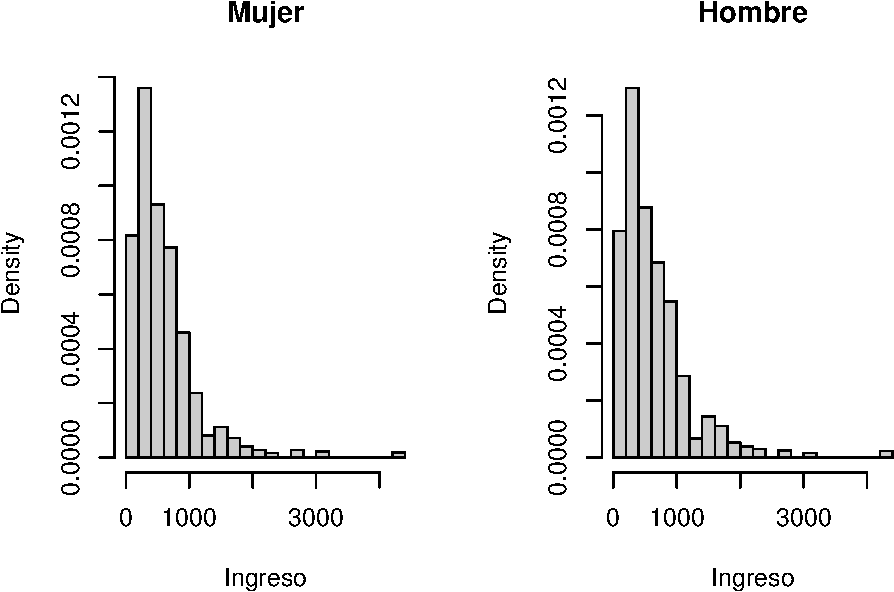
\includegraphics{04-Continuas_files/figure-latex/unnamed-chunk-3-1.pdf}

Como se puede observar, los argumentos utilizando para realizar los gráficos son los mismo que se utilizaron y ejemplificaron anteriormente. Cabe notar que la función \emph{subset} permite hacer un subconjunto de la población, que para nuetro caso son aquellos hombres y mujeres mayores o iguales a 18 años.

Si el objetivo ahora es realizar análisis de localización y variablidad, por ejemplo, graficar Bloxplot teniendo en cuenta los factores de expansión, a continuación, se muestran las sintaxis de como realizarlo en \texttt{R}.

\begin{Shaded}
\begin{Highlighting}[]
\NormalTok{sub\_Urbano }\OtherTok{\textless{}{-}}\NormalTok{ diseno }\SpecialCharTok{\%\textgreater{}\%}  \FunctionTok{filter}\NormalTok{(Zone }\SpecialCharTok{==} \StringTok{"Urban"}\NormalTok{)}
\NormalTok{sub\_Rural  }\OtherTok{\textless{}{-}}\NormalTok{ diseno }\SpecialCharTok{\%\textgreater{}\%}  \FunctionTok{filter}\NormalTok{(Zone }\SpecialCharTok{==} \StringTok{"Rural"}\NormalTok{)}

\FunctionTok{par}\NormalTok{(}\AttributeTok{mfrow =} \FunctionTok{c}\NormalTok{(}\DecValTok{1}\NormalTok{,}\DecValTok{2}\NormalTok{))}
\FunctionTok{svyboxplot}\NormalTok{(}
\NormalTok{  Income}\SpecialCharTok{\textasciitilde{}}\DecValTok{1}\NormalTok{ ,}
\NormalTok{  sub\_Urbano,}
  \AttributeTok{col =} \StringTok{"grey80"}\NormalTok{,}
  \AttributeTok{ylab =} \StringTok{"Ingreso"}\NormalTok{,}
  \AttributeTok{xlab =} \StringTok{"Urbano"}\NormalTok{)}

\FunctionTok{svyboxplot}\NormalTok{(}
\NormalTok{  Income }\SpecialCharTok{\textasciitilde{}} \DecValTok{1}\NormalTok{ ,}
\NormalTok{  sub\_Rural,}
  \AttributeTok{col =} \StringTok{"grey80"}\NormalTok{,}
  \AttributeTok{ylab =} \StringTok{"Ingreso"}\NormalTok{,}
  \AttributeTok{xlab =} \StringTok{"Rural"}\NormalTok{)}
\end{Highlighting}
\end{Shaded}

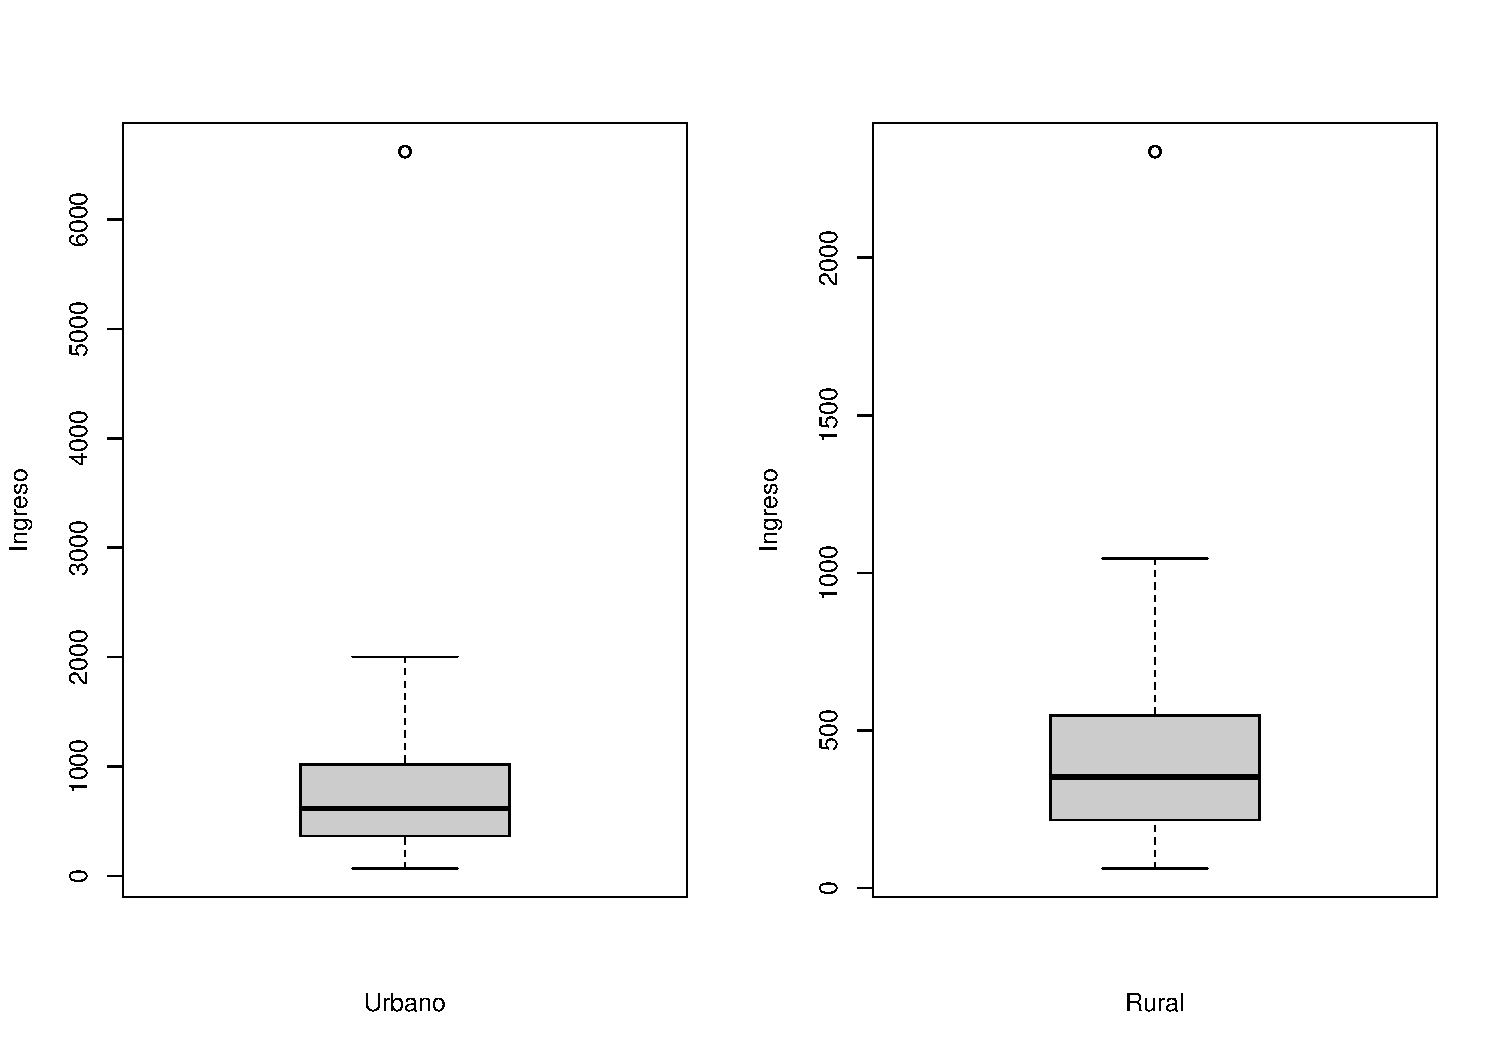
\includegraphics{04-Continuas_files/figure-latex/box1-1.pdf}

Los argumentos usados en la función \emph{svyboxplot} para generar el gráfico son muy similares a los usados en la función \emph{svyhist}. Algo a recalcar el los argumentos de esta función es que el símbolo ``Income \textasciitilde{} 1'' hace referencia a que todas las personas pertenecen a un solo grupo que puede ser urbano o rural dependiendo del caso y por eso se requiere indicarle a \texttt{R} esa restricción, lo cual se hace con el símbolo ``\textasciitilde1''.

\hypertarget{estimaciuxf3n-puntual}{%
\section{Estimación puntual}\label{estimaciuxf3n-puntual}}

Después de realizar el análisis gráfico de las tendencias de las variables continuas de la encuesta, es necesario obtener las estimaciones puntuales de los parámetros que se midieron. Dichas estimaciones se obtienen de forma general o desagregado por niveles de acuerdo con las necesidades de la investigación. Entiéndase como estimaciones puntuales en el contexto de las encuestas de hogares a la estimación de totales, pormedios, razones, etc. Como lo menciona \textbf{Heeringa, et al (2017)} la estimación del total o promedio de una población y su varianza muestral ha jugado un papel muy importante en el desarrollo de la teoría del muestreo probabilístico, particularmente en las encuestas de hogares dado que, permiten dar un valor muy acertado de lo que puede estar pasando en los hogares estudiados y con ello tomar decisiones de política publica de manera informada.

\hypertarget{estimaciuxf3n-de-totales-e-intervalos-de-confianza}{%
\subsection{Estimación de totales e intervalos de confianza}\label{estimaciuxf3n-de-totales-e-intervalos-de-confianza}}

Una vez definido el diseño muestral, lo cual se hizo en la sección anterior), se procede a realizar los procesos de estimación de los parámetros de interés. Para efectos de este texto se iniciará con la estimación del total de los ingresos de los hogares.

En su mayoría, los paquetes estadístico actuales no utilizan técnicas avanzadas para estimar los totales de la población, por ejemplo, usar estimadores generales de regresión (GREG) o métodos de calibración. Sin embargo, \textbf{Valiente et al.~(2000)} realizó una librería implementada en \emph{S-plus} que premite realizar estos procedimientos de estimación, que se pueden escribir de manera sencilla en códigos en R \textbf{(Valliant et al., 2013)}.

Para la estimación de totales con diseños muestrales complejos que incluya estratificación \(\left(h=1,2,...,H\right)\)y muestreo por conglomerados (cuyos conglomerados están dentro del estrato \(h\)) indexados por \(\alpha=1,2,...,a_{h}\), el estimador para el total se puede escribir como:

\begin{eqnarray*}
\hat{Y}_{\omega} & = & \sum_{h=1}^{H}\sum_{\alpha=1}^{a_{h}}\sum_{i=1}^{n_{h\alpha}}\omega_{h\alpha i}y_{h\alpha i}.
\end{eqnarray*}

El estimador insesgado de la varianza para este estimador es:

\begin{eqnarray*}
var\left(\hat{Y}_{\omega}\right) & = & \sum_{h=1}^{H}\frac{a_{h}}{\left(a_{h}-1\right)}\left[\sum_{\alpha=1}^{a_{h}}\left(\sum_{i=1}^{n_{h\alpha}}\omega_{h\alpha i}y_{h\alpha i}\right)^{2}-\frac{\left({ \sum_{\alpha=1}^{a_{h}}}\omega_{h\alpha i}y_{h\alpha i}\right)^{2}}{a_{h}}\right]
\end{eqnarray*}

Como se puede observar, calcular la estimación del total y su varianza estimada es complejo. Sin embargo, dichos cálculos se pueden hacer en \texttt{R} mediante la función \texttt{svytotal} y el intervalos de confianza se calcula con la función \texttt{confint}, ambos usando la librería \texttt{survey}. A continuación, se muestran los códigos:

\begin{Shaded}
\begin{Highlighting}[]
\NormalTok{total\_Ingresos}\OtherTok{\textless{}{-}} \FunctionTok{svytotal}\NormalTok{(}\SpecialCharTok{\textasciitilde{}}\NormalTok{Income, diseno, }\AttributeTok{deff=}\NormalTok{T, )}
\NormalTok{total\_Ingresos}
\end{Highlighting}
\end{Shaded}

\begin{verbatim}
##           total       SE DEff
## Income 85793667  4778674   11
\end{verbatim}

\begin{Shaded}
\begin{Highlighting}[]
\FunctionTok{confint}\NormalTok{(total\_Ingresos, }\AttributeTok{level =} \FloatTok{0.95}\NormalTok{)}
\end{Highlighting}
\end{Shaded}

\begin{verbatim}
##           2.5 %   97.5 %
## Income 76427637 95159697
\end{verbatim}

Los argumentos que utiliza de la función \texttt{svytotal} con muy sencillos. Para el ejemplo, se le introduce primero la variable en la cual está la información que se desea estimar (Income). Posterior a esto, se introduce el diseño muestral del cual proviene la muestra y, por último, se indica si desea que se reporte el deff de la estimación o no.

Por otro lado, para el cálculo del intervalo de confianza, lo único que requiere es indicarle a la función \texttt{confint} el estimador y la confianza requerida.

Paras seguir ilustrando el uso de la función \texttt{svytotal} y de \texttt{confint}, estimemos el total de gastos de los hogares, pero ahora el intervalo de confianza se calculará al 90\% de confianza. Los siguientes códigos realizan las estimaciones:

\begin{Shaded}
\begin{Highlighting}[]
\NormalTok{total\_gastos}\OtherTok{\textless{}{-}} \FunctionTok{svytotal}\NormalTok{ (}\SpecialCharTok{\textasciitilde{}}\NormalTok{Expenditure, diseno, }\AttributeTok{deff=}\NormalTok{T) }
\NormalTok{total\_gastos}
\end{Highlighting}
\end{Shaded}

\begin{verbatim}
##                total       SE   DEff
## Expenditure 55677504  2604138 10.222
\end{verbatim}

\begin{Shaded}
\begin{Highlighting}[]
\FunctionTok{confint}\NormalTok{(total\_gastos, }\AttributeTok{level =} \FloatTok{0.9}\NormalTok{)}
\end{Highlighting}
\end{Shaded}

\begin{verbatim}
##                  5 %     95 %
## Expenditure 51394077 59960931
\end{verbatim}

Si el objetivo ahora es estimar el total de los ingreso de los hogares pero discriminado por sexo, se utilizará ahora la función \texttt{cascade}de la libraría \texttt{srvyr}, la cual permite agregar
la suma de las categorías al final la tabla. También se utilizará la función \texttt{group\_by} la cual permite obtener resultados agrupados por los niveles de interés.

\begin{Shaded}
\begin{Highlighting}[]
\NormalTok{diseno }\SpecialCharTok{\%\textgreater{}\%} \FunctionTok{group\_by}\NormalTok{(Sex) }\SpecialCharTok{\%\textgreater{}\%}
  \FunctionTok{cascade}\NormalTok{(}\AttributeTok{Total =} \FunctionTok{survey\_total}\NormalTok{(}
\NormalTok{    Income, }\AttributeTok{level =} \FloatTok{0.95}\NormalTok{,}
    \AttributeTok{vartype =}  \FunctionTok{c}\NormalTok{(}\StringTok{"se"}\NormalTok{, }\StringTok{"ci"}\NormalTok{)),}
          \AttributeTok{.fill =} \StringTok{"Total ingreso"}\NormalTok{)}
\end{Highlighting}
\end{Shaded}

\begin{verbatim}
## # A tibble: 3 x 5
##   Sex               Total Total_se Total_low Total_upp
##   <chr>             <dbl>    <dbl>     <dbl>     <dbl>
## 1 Female        44153820. 2324452. 39551172. 48756467.
## 2 Male          41639847. 2870194. 35956576. 47323118.
## 3 Total ingreso 85793667. 4778674. 76331414. 95255920.
\end{verbatim}

Como se pudo observar en lo códigos anteriores, otra forma de obtener las estimaciones del total, su desviación estándar y el intervalo de confianza es usando el argumento \texttt{vartype} e indicándole las opciones ``se'', ``ci'' respectivamente.

\hypertarget{estimaciuxf3n-de-la-media-e-intervalo-de-confianza}{%
\subsection{Estimación de la media e intervalo de confianza}\label{estimaciuxf3n-de-la-media-e-intervalo-de-confianza}}

La estimación de la media poblacional es un parámetro muy importante en las encuestas de hogares, dado que, por ejemplo, uno de los indicadores trazadores en este tipo de encuestas son los ingresos medios por hogar. Además, este tipo de parámetros no permiten describir y analizar las tendencias centrales de estas variables en poblaciones de interés. Según \textbf{Gutiérrez (2016)} un estimador de la media poblacional se puede escribir como una razón no lineal de dos totales de población finitas estimados como sigue:

\begin{eqnarray*}
\bar{Y}_{\omega} & = & \frac{\sum_{h=1}^{H}\sum_{\alpha=1}^{a_{h}}\sum_{i=1}^{n_{h\alpha}}\omega_{h\alpha i}y_{h\alpha i}}{\sum_{h=1}^{H}\sum_{\alpha=1}^{a_{h}}\sum_{i=1}^{n_{h\alpha}}\omega_{h\alpha i}}\\
 & = & \frac{\hat{Y}}{\hat{N}}.
\end{eqnarray*}

Como una observación tenga en cuenta que, si \(y\) es una variable
binaria, la media ponderada estima la proporción de la población.
Por otro lado, como \(\bar{Y}_{\omega}\) no es una estadística lineal,
no existe una fórmula cerrada para la varianza de este estimador.
Es por lo anterior que, se deben recurrir a usar métodos de remuestreo
o series de Taylor. Para este caso en particular, usando series de
Taylor el estimador insesgado de la varianza para este estimador es:

\begin{eqnarray*}
var\left(\bar{Y}_{\omega}\right) & \dot{=} & \frac{var\left(\hat{Y}\right)+\bar{Y}_{\omega}^{2}\times var\left(\hat{N}\right)-2\times\bar{Y}_{\omega}\times cov\left(\hat{Y},\hat{N}\right)}{\hat{N}^{2}}
\end{eqnarray*}

Como se puede observar, el cálculo de la estimación de la varianza tiene componentes complejos de calcular de manera analítica, como la covarianza entre el total estimado y el tamaño poblacional estimado. Sin embargo, \texttt{R} tiene funciones que incorpora estos estimadores. A continuación, se presenta la sintaxis para hacer dichos cálculos.

\begin{Shaded}
\begin{Highlighting}[]
\NormalTok{Media\_ingresos}\OtherTok{\textless{}{-}} \FunctionTok{svymean}\NormalTok{(}\SpecialCharTok{\textasciitilde{}}\NormalTok{Income, diseno, }\AttributeTok{deff=}\NormalTok{T) }
\NormalTok{Media\_ingresos}
\end{Highlighting}
\end{Shaded}

\begin{verbatim}
##           mean      SE   DEff
## Income 570.945  28.478 8.8211
\end{verbatim}

\begin{Shaded}
\begin{Highlighting}[]
\FunctionTok{confint}\NormalTok{(Media\_ingresos, }\AttributeTok{level =} \FloatTok{0.95}\NormalTok{)}
\end{Highlighting}
\end{Shaded}

\begin{verbatim}
##           2.5 %   97.5 %
## Income 515.1299 626.7607
\end{verbatim}

Como se puede observar, los argumentos que utiliza la función \texttt{svymean} para realizar la estimación de la media de los ingresos de los hogares y la desviación estándar estimada del estimador son similares a los utilizando con la función \texttt{svytotal}. Similarmente ocurre con el intervalo de confianza.

Por otro lado, tal como se realizó con el total, a manera de ejemplo, se estima la media de los gastos en los hogares como sigue a continuación:

\begin{Shaded}
\begin{Highlighting}[]
\NormalTok{Media\_gastos}\OtherTok{\textless{}{-}} \FunctionTok{svymean}\NormalTok{ (}\SpecialCharTok{\textasciitilde{}}\NormalTok{Expenditure, diseno, }\AttributeTok{deff=}\NormalTok{T)}
\NormalTok{Media\_gastos}
\end{Highlighting}
\end{Shaded}

\begin{verbatim}
##                mean      SE   DEff
## Expenditure 370.526  13.294 6.0156
\end{verbatim}

\begin{Shaded}
\begin{Highlighting}[]
\FunctionTok{confint}\NormalTok{(Media\_gastos)}
\end{Highlighting}
\end{Shaded}

\begin{verbatim}
##                2.5 %   97.5 %
## Expenditure 344.4697 396.5829
\end{verbatim}

También se pueden realizar estimaciones de la media por subgrupos siguiendo el mismo esquema mostrado para la función \texttt{svytotal}. Particularmente, los gastos de los hogares discriminados por sexo es:

\begin{Shaded}
\begin{Highlighting}[]
\NormalTok{diseno }\SpecialCharTok{\%\textgreater{}\%} \FunctionTok{group\_by}\NormalTok{(Sex) }\SpecialCharTok{\%\textgreater{}\%}
  \FunctionTok{cascade}\NormalTok{(}
    \AttributeTok{Media =} \FunctionTok{survey\_mean}\NormalTok{(}
\NormalTok{      Expenditure, }\AttributeTok{level =} \FloatTok{0.95}\NormalTok{,}
       \AttributeTok{vartype =}  \FunctionTok{c}\NormalTok{(}\StringTok{"se"}\NormalTok{, }\StringTok{"ci"}\NormalTok{)), }
        \AttributeTok{.fill =} \StringTok{"El gasto medio"}\NormalTok{  ) }\SpecialCharTok{\%\textgreater{}\%}
  \FunctionTok{arrange}\NormalTok{(}\FunctionTok{desc}\NormalTok{(Sex))}
\end{Highlighting}
\end{Shaded}

\begin{verbatim}
## # A tibble: 3 x 5
##   Sex            Media Media_se Media_low Media_upp
##   <chr>          <dbl>    <dbl>     <dbl>     <dbl>
## 1 Male            374.     16.1      343.      406.
## 2 Female          367.     12.3      343.      391.
## 3 El gasto medio  371.     13.3      344.      397.
\end{verbatim}

Por zona,

\begin{Shaded}
\begin{Highlighting}[]
\NormalTok{diseno }\SpecialCharTok{\%\textgreater{}\%} \FunctionTok{group\_by}\NormalTok{(Zone) }\SpecialCharTok{\%\textgreater{}\%}
  \FunctionTok{cascade}\NormalTok{(}
    \AttributeTok{Media =} \FunctionTok{survey\_mean}\NormalTok{(}
\NormalTok{      Expenditure, }\AttributeTok{level =} \FloatTok{0.95}\NormalTok{,}
       \AttributeTok{vartype =}  \FunctionTok{c}\NormalTok{(}\StringTok{"se"}\NormalTok{, }\StringTok{"ci"}\NormalTok{)), }
        \AttributeTok{.fill =} \StringTok{"El gasto medio"}\NormalTok{)}\SpecialCharTok{\%\textgreater{}\%}
  \FunctionTok{arrange}\NormalTok{(}\FunctionTok{desc}\NormalTok{(Zone))}
\end{Highlighting}
\end{Shaded}

\begin{verbatim}
## # A tibble: 3 x 5
##   Zone           Media Media_se Media_low Media_upp
##   <chr>          <dbl>    <dbl>     <dbl>     <dbl>
## 1 Urban           460.     22.2      416.      504.
## 2 Rural           274.     10.3      254.      294.
## 3 El gasto medio  371.     13.3      344.      397.
\end{verbatim}

Por sexo y zona,

\begin{Shaded}
\begin{Highlighting}[]
\NormalTok{diseno }\SpecialCharTok{\%\textgreater{}\%} \FunctionTok{group\_by}\NormalTok{(Zone, Sex) }\SpecialCharTok{\%\textgreater{}\%}
  \FunctionTok{cascade}\NormalTok{(}
    \AttributeTok{Media =} \FunctionTok{survey\_mean}\NormalTok{(}
\NormalTok{      Expenditure, }\AttributeTok{level =} \FloatTok{0.95}\NormalTok{,}
       \AttributeTok{vartype =}  \FunctionTok{c}\NormalTok{(}\StringTok{"se"}\NormalTok{, }\StringTok{"ci"}\NormalTok{)),}
        \AttributeTok{.fill =} \StringTok{"El gasto medio"}\NormalTok{) }\SpecialCharTok{\%\textgreater{}\%}
  \FunctionTok{arrange}\NormalTok{(}\FunctionTok{desc}\NormalTok{(Zone), }\FunctionTok{desc}\NormalTok{(Sex)) }\SpecialCharTok{\%\textgreater{}\%}
  \FunctionTok{data.frame}\NormalTok{()}
\end{Highlighting}
\end{Shaded}

\begin{verbatim}
##             Zone            Sex    Media Media_se Media_low Media_upp
## 1          Urban           Male 469.8124 26.96068  416.4276  523.1973
## 2          Urban         Female 450.8151 20.11853  410.9784  490.6518
## 3          Urban El gasto medio 459.6162 22.20655  415.6450  503.5874
## 4          Rural           Male 275.3018 10.24848  255.0088  295.5948
## 5          Rural         Female 272.6769 11.61470  249.6786  295.6751
## 6          Rural El gasto medio 273.9461 10.26141  253.6275  294.2647
## 7 El gasto medio El gasto medio 370.5263 13.29444  344.2020  396.8506
\end{verbatim}

\hypertarget{estimaciuxf3n-de-medidas-de-dispersiuxf3n-y-localizaciuxf3n}{%
\subsection{Estimación de medidas de dispersión y localización}\label{estimaciuxf3n-de-medidas-de-dispersiuxf3n-y-localizaciuxf3n}}

En las encuestas de hogares siempre es necesario estimar medidas de dispersión de las variables estudiadas. Esto con el fin de, por ejemplo, ver qué tan disímiles son los ingresos medios de los hogares en un país determinado y con esto poder tomar acciones de política pública. Por lo anterior, es importante estudiar este parámetro en este texto. A continuación, se presenta el estimador de la desviación estándar:

\begin{eqnarray}
s\left(y\right){}_{\omega} & = & \frac{\sum_{h=1}^{H}\sum_{\alpha=1}^{a_{h}}\sum_{i=1}^{n_{h\alpha}}\omega_{h\alpha i}\left(y_{h\alpha i}-\bar{Y}_{\omega}\right)^{2}}{\sum_{h=1}^{H}\sum_{\alpha=1}^{a_{h}}\sum_{i=1}^{n_{h\alpha}}\omega_{h\alpha i}-1}
\end{eqnarray}

Para llevar a cabo la estimación en \texttt{R} de la desviación estándar en encuestas de hogares, se utilizan la función \texttt{survey\_var} la cual se ejemplifica a continuación:

\begin{Shaded}
\begin{Highlighting}[]
\NormalTok{(sd\_Est }\OtherTok{\textless{}{-}}\NormalTok{ diseno }\SpecialCharTok{\%\textgreater{}\%} \FunctionTok{group\_by}\NormalTok{(Zone) }\SpecialCharTok{\%\textgreater{}\%} 
   \FunctionTok{summarise}\NormalTok{(}\AttributeTok{Sd =} \FunctionTok{sqrt}\NormalTok{(}
  \FunctionTok{survey\_var}\NormalTok{(}
\NormalTok{    Income,}
    \AttributeTok{level =} \FloatTok{0.95}\NormalTok{,}
    \AttributeTok{vartype =}  \FunctionTok{c}\NormalTok{(}\StringTok{"se"}\NormalTok{, }\StringTok{"ci"}\NormalTok{),}
\NormalTok{  ) )))}
\end{Highlighting}
\end{Shaded}

\begin{verbatim}
## # A tibble: 2 x 5
##   Zone     Sd Sd_se Sd_low Sd_upp
##   <chr> <dbl> <dbl>  <dbl>  <dbl>
## 1 Rural  310.  117.   263.   352.
## 2 Urban  582.  285.   422.   707.
\end{verbatim}

Como se pudo ver en el ejemplo anterior, se estimó la desviación estándar de los ingresos por zona reportando el error estándar en la estimación y un intervalo de confianza al 95\%. Los argumentos que utiliza la función \texttt{survey\_var} son similares a los usados en las funciones anteriores para estimar medias y totales.

Si el interés ahora se centra en estimar la desviación estándar clasificando por sexo y zona, los códigos computacionales son los siguientes:

\begin{Shaded}
\begin{Highlighting}[]
\NormalTok{(sd\_Est }\OtherTok{\textless{}{-}}\NormalTok{ diseno }\SpecialCharTok{\%\textgreater{}\%} \FunctionTok{group\_by}\NormalTok{(Zone, Sex) }\SpecialCharTok{\%\textgreater{}\%} 
   \FunctionTok{summarise}\NormalTok{(}\AttributeTok{Sd =} \FunctionTok{sqrt}\NormalTok{(}
  \FunctionTok{survey\_var}\NormalTok{(}
\NormalTok{    Income,}
    \AttributeTok{level =} \FloatTok{0.95}\NormalTok{,}
    \AttributeTok{vartype =}  \FunctionTok{c}\NormalTok{(}\StringTok{"se"}\NormalTok{, }\StringTok{"ci"}\NormalTok{),}
\NormalTok{   )}
\NormalTok{))) }\SpecialCharTok{\%\textgreater{}\%} \FunctionTok{data.frame}\NormalTok{()}
\end{Highlighting}
\end{Shaded}

\begin{verbatim}
##    Zone    Sex       Sd    Sd_se   Sd_low   Sd_upp
## 1 Rural Female 294.8683 111.6203 249.5537 334.0921
## 2 Rural   Male 325.7584 124.9643 274.2209 370.1890
## 3 Urban Female 568.3920 286.4585 400.7312 696.8166
## 4 Urban   Male 596.7756 288.9435 436.8362 722.1194
\end{verbatim}

Las medidas de posición no central (Percentiles) se diseñaron con el fin de conocer otros puntos característicos de la distribución de los datos que no son los valores centrales. Entre las medidas de posición no central más importantes están la mediana, cuartiles y percentiles. En la mayoría de las encuestas de hogares no solo estiman totales, medias y proporciones. En algunos indicadores es necesario estimar otros parámetros, por ejemplo, medianas y percentiles. Como lo menciona \textbf{Tellez et al (2015)} la mediana una medida de tendencia central la cual, a diferencia del promedio, no es fácilmente influenciada por datos atípicos y, por esto, se conoce como una medida robusta. La mediana es el valor que divide la población en dos partes iguales. Lo que implica que, la mitad de las observaciones de la característica de interés está por encima de la media y la otra mitad está por debajo.

Por otro lado, la estimación de percentiles de ingresos en un país determinado puede definir el inicio de una política pública. por ejemplo, poner a tributar aquellas personas naturales que son el 10\% más alto de la distribución de los ingresos o por el contrario, generar subsidios de transporte a aquellas familias que están en el 15\% inferior de la distribución de los ingresos.

La estimación de cuantiles \textbf{(Loomis et al., 2005)} se basa en los resultados relacionados con el estimador ponderado para totales, empleando una estimación de la función de distribución (CDF, por sus siglas en inglés) acumulada de la población. Específicamente, la CDF para una variable y en una población finita dada de tamaño \(N\) se define de la siguiente manera:

\begin{eqnarray*}
F\left(x\right) & = & \frac{{ \sum_{i=1}^{N}}I\left(y_{i}\leq x\right)}{N}
\end{eqnarray*}

Donde, \(I\left(y_{i}\leq x\right)\) es una variable indicadora la
cual es igual a 1 si \(y_{i}\) es menor o igual a un valor específico
\(x\), 0 en otro caso. Un estimador de la CDF en un diseño complejo
(encuesta de hogares) de tamaño \(n\) está dado por:

\begin{eqnarray*}
\hat{F}\left(x\right) & = & \frac{\sum_{h=1}^{H}\sum_{\alpha=1}^{a_{h}}\sum_{i=1}^{n_{h\alpha}}\omega_{h\alpha i}I\left(y_{i}\leq x\right)}{\sum_{h=1}^{H}\sum_{\alpha=1}^{a_{h}}\sum_{i=1}^{n_{h\alpha}}\omega_{h\alpha i}}
\end{eqnarray*}

Una vez estimada la CDF utilizando los pesos del diseño muestral, el cuantil q-ésimo de una variable \(y\) es el valor más pequeño de \(y\) tal que la CDF de la población es mayor o igual que \(q\). Como es bien sabido, la mediana es aquel valor donde la CDF es mayor o igual a 0.5 y, por tanto, la media estimada es aquel valor donde la estimación de CDF es mayor o igual a 0.5.

Siguiendo las recomendaciones de \emph{Heeringa et al (2017)} para estimar cuantiles, primero se considera las estadísticas de orden que se denotan como \(y_{1},\ldots,y_{n}\), y encuentra el valor de \(j\) \((j=1,\ldots,n)\) tal que:

\begin{eqnarray*}
 & \hat{F}\left(y_{j}\right)\leq q\leq\hat{F}\left(y_{j+1}\right)
\end{eqnarray*}

Ahora bien, la estimación del q-ésimo cuantil \(Y_{q}\) en un diseño de muestreo complejo está dado por:

\begin{eqnarray*}
\hat{Y}_{q} & = & y_{j}+\frac{q-\hat{F}\left(y_{j}\right)}{\hat{F}\left(y_{j+1}\right)-\hat{F}\left(y_{j}\right)}\left(y_{j+1}-y_{j}\right)
\end{eqnarray*}

Para la estimación de la varianza e intervalos de confianza de cuantiles, \textbf{Kovar et al.~(1988)} muestra los resultados de un estudio de simulación en donde recomienda el uso de Balanced Repeated Replication (BRR) para estimarla.

Los estimadores y procedimientos antes mencionados para la estimación de percentiles y sus varianzas están implementados en \texttt{R}. Particularmente, la estimación de la mediana se realiza usando la función \texttt{survey\_median}. A continuación, se muestra la sintaxis de cómo calcular la mediana de los gastos, la desviación estándar y el intervalo de confianza al 95\% de los hogares en la base de datos de ejemplo.

\begin{Shaded}
\begin{Highlighting}[]
\NormalTok{diseno }\SpecialCharTok{\%\textgreater{}\%} \FunctionTok{summarise}\NormalTok{(}\AttributeTok{Mediana =} 
  \FunctionTok{survey\_median}\NormalTok{(}
\NormalTok{    Expenditure,}
    \AttributeTok{level =} \FloatTok{0.95}\NormalTok{,}
    \AttributeTok{vartype =}  \FunctionTok{c}\NormalTok{(}\StringTok{"se"}\NormalTok{, }\StringTok{"ci"}\NormalTok{),}
\NormalTok{   ))}
\end{Highlighting}
\end{Shaded}

\begin{verbatim}
## # A tibble: 1 x 4
##   Mediana Mediana_se Mediana_low Mediana_upp
##     <dbl>      <dbl>       <dbl>       <dbl>
## 1    298.       8.83        282.        317.
\end{verbatim}

Como se puede observar, los argumentos de la función \texttt{survey\_median} son similares a los del total y la media.

Ahora bien, al igual que con los demás parámetros, si el objetivo ahora es estimar la mediana de los gastos de los hogares, pero esta vez discriminada por zona y también por sexo, el código computacional sería el siguiente:

\begin{Shaded}
\begin{Highlighting}[]
\NormalTok{diseno }\SpecialCharTok{\%\textgreater{}\%} \FunctionTok{group\_by}\NormalTok{(Zone) }\SpecialCharTok{\%\textgreater{}\%} 
  \FunctionTok{summarise}\NormalTok{(}\AttributeTok{Mediana =} 
  \FunctionTok{survey\_median}\NormalTok{(}
\NormalTok{    Expenditure,}
    \AttributeTok{level =} \FloatTok{0.95}\NormalTok{,}
    \AttributeTok{vartype =}  \FunctionTok{c}\NormalTok{(}\StringTok{"se"}\NormalTok{, }\StringTok{"ci"}\NormalTok{),}
\NormalTok{   ))}
\end{Highlighting}
\end{Shaded}

\begin{verbatim}
## # A tibble: 2 x 5
##   Zone  Mediana Mediana_se Mediana_low Mediana_upp
##   <chr>   <dbl>      <dbl>       <dbl>       <dbl>
## 1 Rural    241.       11.0        214.        258.
## 2 Urban    381.       19.8        337.        416.
\end{verbatim}

\begin{Shaded}
\begin{Highlighting}[]
\NormalTok{diseno }\SpecialCharTok{\%\textgreater{}\%} \FunctionTok{group\_by}\NormalTok{(Sex) }\SpecialCharTok{\%\textgreater{}\%} 
  \FunctionTok{summarise}\NormalTok{(}\AttributeTok{Mediana =} 
  \FunctionTok{survey\_median}\NormalTok{(}
\NormalTok{    Expenditure,}
    \AttributeTok{level =} \FloatTok{0.95}\NormalTok{,}
    \AttributeTok{vartype =}  \FunctionTok{c}\NormalTok{(}\StringTok{"se"}\NormalTok{, }\StringTok{"ci"}\NormalTok{),}
\NormalTok{   ))}
\end{Highlighting}
\end{Shaded}

\begin{verbatim}
## # A tibble: 2 x 5
##   Sex    Mediana Mediana_se Mediana_low Mediana_upp
##   <chr>    <dbl>      <dbl>       <dbl>       <dbl>
## 1 Female    300.      10.5         282.        324.
## 2 Male      297.       9.29        277.        314.
\end{verbatim}

Si el objetivo ahora es estimar cuantiles, por ejemplo, el cuantil 0.25 de los gastos de los hogares, se realizaría usando la función \texttt{survey\_quantile} como sigue:

\begin{Shaded}
\begin{Highlighting}[]
\NormalTok{diseno }\SpecialCharTok{\%\textgreater{}\%} 
  \FunctionTok{summarise}\NormalTok{(}
    \AttributeTok{Q =}  \FunctionTok{survey\_quantile}\NormalTok{(}
\NormalTok{    Expenditure,}
    \AttributeTok{quantiles =} \FloatTok{0.5}\NormalTok{,}
    \AttributeTok{level =} \FloatTok{0.95}\NormalTok{,}
    \AttributeTok{vartype =}  \FunctionTok{c}\NormalTok{(}\StringTok{"se"}\NormalTok{, }\StringTok{"ci"}\NormalTok{),}
    \AttributeTok{interval\_type =} \StringTok{"score"}
\NormalTok{   ))}
\end{Highlighting}
\end{Shaded}

\begin{verbatim}
## # A tibble: 1 x 4
##   Q_q50 Q_q50_se Q_q50_low Q_q50_upp
##   <dbl>    <dbl>     <dbl>     <dbl>
## 1  298.     12.0      265.      312.
\end{verbatim}

si ahora se desea estimar el cuantil 0.25 pero discriminando por sexo y por zona se realizaría como sigue:

\begin{Shaded}
\begin{Highlighting}[]
\NormalTok{diseno }\SpecialCharTok{\%\textgreater{}\%} \FunctionTok{group\_by}\NormalTok{(Sex) }\SpecialCharTok{\%\textgreater{}\%} 
  \FunctionTok{summarise}\NormalTok{(}
    \AttributeTok{Q =}  \FunctionTok{survey\_quantile}\NormalTok{(}
\NormalTok{    Expenditure,}
    \AttributeTok{quantiles =} \FloatTok{0.25}\NormalTok{,}
    \AttributeTok{level =} \FloatTok{0.95}\NormalTok{,}
    \AttributeTok{vartype =}  \FunctionTok{c}\NormalTok{(}\StringTok{"se"}\NormalTok{, }\StringTok{"ci"}\NormalTok{),}
    \AttributeTok{interval\_type =} \StringTok{"score"}
\NormalTok{   ))}
\end{Highlighting}
\end{Shaded}

\begin{verbatim}
## # A tibble: 2 x 5
##   Sex    Q_q25 Q_q25_se Q_q25_low Q_q25_upp
##   <chr>  <dbl>    <dbl>     <dbl>     <dbl>
## 1 Female  210.     14.9      169.      228.
## 2 Male    193.     10.4      163.      205.
\end{verbatim}

\begin{Shaded}
\begin{Highlighting}[]
\NormalTok{diseno }\SpecialCharTok{\%\textgreater{}\%} \FunctionTok{group\_by}\NormalTok{(Zone) }\SpecialCharTok{\%\textgreater{}\%} 
  \FunctionTok{summarise}\NormalTok{(}
    \AttributeTok{Q =}  \FunctionTok{survey\_quantile}\NormalTok{(}
\NormalTok{    Expenditure,}
    \AttributeTok{quantiles =} \FloatTok{0.25}\NormalTok{,}
    \AttributeTok{level =} \FloatTok{0.95}\NormalTok{,}
    \AttributeTok{vartype =}  \FunctionTok{c}\NormalTok{(}\StringTok{"se"}\NormalTok{, }\StringTok{"ci"}\NormalTok{),}
    \AttributeTok{interval\_type =} \StringTok{"score"}
\NormalTok{   ))}
\end{Highlighting}
\end{Shaded}

\begin{verbatim}
## # A tibble: 2 x 5
##   Zone  Q_q25 Q_q25_se Q_q25_low Q_q25_upp
##   <chr> <dbl>    <dbl>     <dbl>     <dbl>
## 1 Rural  160.     4.64      145.      163.
## 2 Urban  258.     9.05      256.      292.
\end{verbatim}

\hypertarget{estimaciuxf3n-del-coeficiente-de-ginni-en-encuestas-de-hogares}{%
\section{Estimación del coeficiente de Ginni en encuestas de hogares}\label{estimaciuxf3n-del-coeficiente-de-ginni-en-encuestas-de-hogares}}

Para iniciar esta sección tengamos en cuenta la siguiente reflexión: \emph{Definir lo justo siempre será difícil y es algo a lo que quizá sea poco realista aspirar a conseguir. Sin embargo si estamos un poco más conscientes de cómo la desigualdad afecta nuestra libertad y cómo se refleja en el bienestar y calidad de vida de las personas, podremos poner en contexto una discusión que tendremos cada vez más presente en el mundo y en el país.}

La desigualdad en todos los aspectos es un problema más comunes en todos los países del mundo. Particularmente, la desigualdad económica es un problema que atañe a muchas instituciones internacionales como, por ejemplo, Naciones Unidas quien tiene este problema detectado en los Objetivos de Desarrollo Sostenibles (ODS, por sus siglas). Dado lo anterior, es clave poder medir la desigualdad económica de los hogares en los países y para esto, el indicador más utilizado es el coeficiente de Gini (CG). El valor del índice de Gini se encuentra entre 0 y 1. Un valor del coeficiente de Gini de \(G = 0\) indica perfecta igualdad en la distribución de la riqueza, con valores más grandes significa una desigualdad cada vez mayor en la distribución de la riqueza. Siguiendo la ecuación de estimación de \emph{Binder y Kovacevic (1995)}, un estimador del coeficiente de Gini es:

\begin{eqnarray*}
\hat{G}\left(y\right) & = & \frac{2\times\sum_{h=1}^{H}\sum_{\alpha=1}^{a_{h}}\sum_{i=1}^{n_{h\alpha}}\omega_{h\alpha i}^{*}\hat{F}_{h\alpha i}y_{h\alpha i}-1}{\bar{y}_{\omega}}
\end{eqnarray*}

Donde,

\begin{itemize}
\item
  \(\omega_{h\alpha i}^{*}=\frac{\omega_{h\alpha i}}{\sum_{h=1}^{H}\sum_{\alpha=1}^{a_{h}}\sum_{i=1}^{n_{h\alpha}}\omega_{h\alpha i}}\).
\item
  \(\hat{F}_{h\alpha i}=\) La estimación de la CDF en el conglomerado \(\alpha\) en el estrato \(h\).
\item
  \(\bar{y}_{\omega}=\) La estimación del promedio.
\end{itemize}

Para calcular el índice de Gini y su varianza estimada en una encuesta de hogares, \texttt{R} tiene cargados los procedimientos en la librería \texttt{convey}. A continuación, se muestra la sintaxis de cómo se realiza la estimación del índice de Gini para los hogares en la base de ejemplo de este capítulo.

\begin{Shaded}
\begin{Highlighting}[]
\FunctionTok{library}\NormalTok{(convey)}
\NormalTok{ diseno\_gini }\OtherTok{\textless{}{-}} \FunctionTok{convey\_prep}\NormalTok{(diseno)}
\FunctionTok{svygini}\NormalTok{( }\SpecialCharTok{\textasciitilde{}}\NormalTok{Income, }\AttributeTok{design =}\NormalTok{ diseno\_gini) }\SpecialCharTok{\%\textgreater{}\%}
  \FunctionTok{data.frame}\NormalTok{()}
\end{Highlighting}
\end{Shaded}

\begin{verbatim}
##             gini    Income
## Income 0.4132757 0.0186633
\end{verbatim}

En primer lugar, se carga el diseño de muestreo con la función \texttt{convey\_prep}. Luego, se estima el índice Gini con la función \texttt{svygini}. En los argumentos de esta última función se introducen la variable ingresos y el diseño muestral complejo.

Por otro lado, si el interés ahora es estimar la \textbf{curva de Lorenz}. La cual, según \emph{Kovacevic, M. S. et. al (1997)} para una distribución dada de ingresos, traza el porcentaje acumulado de la población (desplegado desde el más pobre hasta el más rico) frente a su participación en el ingreso total. El área entre la curva de Lorenz y la línea de 45 grados se conoce como el área de Lorenz. El índice de Gini es igual al doble del área de Lorenz. Una población con la curva de Lorenz más cerca de la línea de 45 grados tiene una distribución de ingresos más equitativa. Si todos los ingresos son iguales, la curva de Lorenz degenera a la línea de 45 grados.

Para realizar la curva de Lorenz en \texttt{R} se utiliza la función \texttt{svylorenz}. A continuación, se muestran los códigos computacionales para realizar la curva de Lorenz para los ingresos:

\begin{Shaded}
\begin{Highlighting}[]
\FunctionTok{library}\NormalTok{(convey)}
\FunctionTok{svylorenz}\NormalTok{(}\AttributeTok{formula =} \SpecialCharTok{\textasciitilde{}}\NormalTok{Income, }
          \AttributeTok{design =}\NormalTok{ diseno\_gini, }
          \AttributeTok{quantiles =} \FunctionTok{seq}\NormalTok{(}\DecValTok{0}\NormalTok{,}\DecValTok{1}\NormalTok{,.}\DecValTok{05}\NormalTok{), }
          \AttributeTok{alpha =}\NormalTok{ .}\DecValTok{01}\NormalTok{ )}
\end{Highlighting}
\end{Shaded}

\begin{center}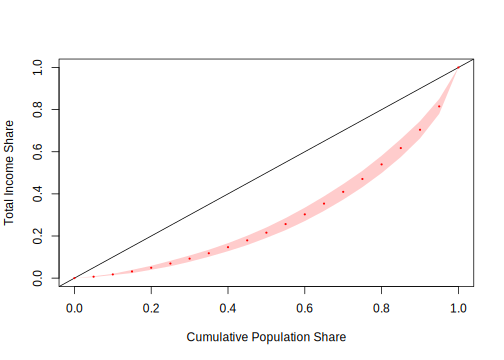
\includegraphics[width=0.7\linewidth]{04-Continuas_files/figure-latex/unnamed-chunk-21-1} \end{center}

\begin{verbatim}
## $quantiles
##        0        0.05        0.1       0.15        0.2       0.25        0.3
## Income 0 0.006819101 0.01759645 0.03165963 0.04922299 0.06943653 0.09258712
##             0.35       0.4      0.45       0.5      0.55       0.6      0.65
## Income 0.1181331 0.1469261 0.1791978 0.2158231 0.2565784 0.3027002 0.3537989
##              0.7      0.75       0.8      0.85       0.9      0.95 1
## Income 0.4096304 0.4706565 0.5398749 0.6174169 0.7042464 0.8151774 1
## 
## $CIs
## , , Income
## 
##        0        0.05        0.1       0.15        0.2       0.25        0.3
## (lower 0 0.006189268 0.01644571 0.02973329 0.04643347 0.06564963 0.08770299
## upper) 0 0.007448933 0.01874718 0.03358597 0.05201251 0.07322343 0.09747124
##             0.35       0.4      0.45       0.5      0.55       0.6      0.65
## (lower 0.1120660 0.1396359 0.1705777 0.2056539 0.2447898 0.2898807 0.3397823
## upper) 0.1242001 0.1542163 0.1878180 0.2259923 0.2683671 0.3155197 0.3678154
##              0.7      0.75       0.8      0.85       0.9      0.95 1
## (lower 0.3943025 0.4542246 0.5227820 0.5991455 0.6835287 0.7983336 1
## upper) 0.4249582 0.4870884 0.5569677 0.6356883 0.7249642 0.8320213 1
\end{verbatim}

Los argumentos que requiere la función son, inicialmente, los ingresos de los hogares y el diseño muestral complejo. Adicionalmente, se definen una secuencia de probabilidades que define la suma de los cuantiles a calcular (quantiles) y por último, un número que especifica el nivel de confianza para el gráfico (alpha).

\hypertarget{anuxe1lisis-de-la-relaciuxf3n-entre-dos-variable-continuas}{%
\section{Análisis de la relación entre dos variable continuas}\label{anuxe1lisis-de-la-relaciuxf3n-entre-dos-variable-continuas}}

En muchos análisis de variables relacionadas con encuestas de hogares no solo basta con analizar el comportamiento de variables de manera individual, por ejemplo, ingresos medios de hombres y mujeres en un país sino también, analizar la diferencia entre los ingresos de los hombres y las mujeres. Esto último con el fin de ir cerrando la brecha salarial que existe.

En este capítulo se estudiará la prueba de hipótesis para diferencia de medias, se darán las herramientas computacionales para estimar razones y contrastes.

\hypertarget{prueba-de-hipuxf3tesis-para-la-diferencia-de-medias-en-encuestas-de-hogares}{%
\section{Prueba de hipótesis para la diferencia de medias en encuestas de hogares}\label{prueba-de-hipuxf3tesis-para-la-diferencia-de-medias-en-encuestas-de-hogares}}

Es llamado prueba de hipótesis a una técnica la cual consiste en hacer una afirmación acerca del valor que el parámetro de la población bajo estudio puede tomar. Esta afirmación puede estar basada en alguna creencia o experiencia pasada que será contrastada con la evidencia que se obtengan a través de la información contenida en la muestra. Como dicha afirmación puede ser o no cierta, dos hipótesis pueden ser planteadas (antagónicas) las cuales se conocen como \(H_{0}:\) Hipótesis nula y \(H_{1}:\) Hipótesis alterna. Si se sospecha que el parámetro \(\theta\) es igual a cierto valor particular \(\theta_{0}\), los posibles juegos de hipótesis a contrastar son:

\[
\begin{cases}
H_{0}: & \theta=\theta_{0}\\
H_{1}: & \theta\neq\theta_{0}
\end{cases}\,\,\,   \begin{cases}
H_{0}: & \theta=\theta_{0}\\
H_{1}: & \theta>\theta_{0}
\end{cases}\,\,\,   \begin{cases}
H_{0}: & \theta=\theta_{0}\\
H_{1}: & \theta<\theta_{0}
\end{cases}
\]

Se dirá que una de las dos hipótesis es cierta solo si la evidencia estadística, la cual es obtenida de la muestra, la apoya. El proceso por medio del cual se escoge una de las dos hipótesis es llamado Prueba de Hipótesis.

En términos generales, algunos parámetros importantes en la estadística descriptivas se pueden escribir como una combinación lineal de medidas de interés. Los casos más usuales son diferencias de medias, sumas ponderadas de medias utilizadas para construir índices económicos, etc.

Considere una función que es una combinación lineal de \(j\) estadísticas descriptivas como se muestra a continuación:

\begin{eqnarray*}
f\left(\theta_{1},\theta_{2},...,\theta_{j}\right) & = & \sum_{j=1}^{J}a_{j}\theta_{j}
\end{eqnarray*}

Una estimación de esta función está dada por:

\begin{eqnarray*}
f\left(\hat{\theta}_{1},\hat{\theta}_{2},...,\hat{\theta}_{j}\right) & = & \sum_{j=1}^{J}a_{j}\hat{\theta}_{j}
\end{eqnarray*}

cuya varianza del estimador se calcula como sigue:

\begin{eqnarray*}
var\left(\sum_{j=1}^{J}a_{j}\hat{\theta}_{j}\right) & = & \sum_{j=1}^{J}a_{j}^{2}var\left(\hat{\theta}_{j}\right)+2\times\sum_{j=1}^{J-1}\sum_{k>j}^{J}a_{j}a_{k}\,cov\left(\hat{\theta}_{j},\hat{\theta}_{k}\right)
\end{eqnarray*}

Como se pudo observar en la ecuación de la varianza del estimador, esta incorpora las varianzas de las estimaciones de los componentes individuales, así como las covarianzas de las estadísticas estimadas.

En primer lugar, una combinación lineal de estadísticas descriptivas de interés en este capítulo es la diferencia de media cuyo parámetro es \({\bar{Y}_{1}-\bar{Y}_{2}}\), donde, \(\bar{Y}_{1}\) es la media de la población 1, por ejemplo, ingresos medios en los hogares obtenido por los padres de familia y \(\bar{Y}_{2}\) es la media de la población 2, que para seguir el ejemplo serían, los ingresos medios de las madres en un hogar.

Considerando el parámetro de interés en esta sección, las hipótesis a estudiar serían las siguientes:

\begin{eqnarray*}
\begin{cases}
H_{0}:\bar{Y}_{1}-\bar{Y}_{2}=0\\
H_{1}:\bar{Y}_{1}-\bar{Y}_{2}\neq0
\end{cases} & \begin{cases}
H_{0}:\bar{Y}_{1}-\bar{Y}_{2}=0\\
H_{1}:\bar{Y}_{1}-\bar{Y}_{2}>0
\end{cases} & \begin{cases}
H_{0}:\bar{Y}_{1}-\bar{Y}_{2}=0\\
H_{1}:\bar{Y}_{1}-\bar{Y}_{2}<0
\end{cases}
\end{eqnarray*}

Para probar estas hipótesis se utiliza el siguiente estadístico de prueba que se distribuye t-student:

\begin{eqnarray*}
t & = & \frac{\bar{Y}_{1}-\bar{Y}_{2}}{se\left(\bar{Y}_{1}-\bar{Y}_{2}\right)},
\end{eqnarray*}

donde,

\begin{eqnarray*}
se\left(\bar{Y}_{1}-\bar{Y}_{2}\right) & = & \sqrt{var\left(\bar{y}_{1}\right)+var\left(\bar{y}_{2}\right)-2cov\left(\bar{y}_{1},\bar{y}_{2}\right)}
\end{eqnarray*}

Si se desea construir un intervalo de confianza para la diferencia de media se realizaría de la siguiente manera:

\begin{eqnarray*}
 & \left(\bar{Y}_{1}-\bar{Y}_{2}\right)\pm t_{gl,\,\alpha/2}\,se\left(\bar{Y}_{1}-\bar{Y}_{2}\right)
\end{eqnarray*}

Para poder llevar a cabo la prueba de hipótesis para la diferencia de media de los ingresos en un hogar por sexo, tomemos la base de datos que tenemos como ejemplo. La función que se encarga de realizar la prueba es \texttt{svyttest} y solo requiere como argumentos la variable ingreso (o variable de interés), la variable sexo (variable discriminadora), el diseño muestral y el nivel de confianza. A continuación, se muestran los códigos computacionales que se requieren:

\begin{Shaded}
\begin{Highlighting}[]
\FunctionTok{svyttest}\NormalTok{(Income }\SpecialCharTok{\textasciitilde{}}\NormalTok{ Sex, }\AttributeTok{design =}\NormalTok{ diseno, }\AttributeTok{level=}\FloatTok{0.95}\NormalTok{) }
\end{Highlighting}
\end{Shaded}

\begin{verbatim}
## 
##  Design-based t-test
## 
## data:  Income ~ Sex
## t = 1.3625, df = 118, p-value = 0.1756
## alternative hypothesis: true difference in mean is not equal to 0
## 95 percent confidence interval:
##  -12.82205  69.38503
## sample estimates:
## difference in mean 
##           28.28149
\end{verbatim}

En esta salida podemos observar que el p-valor de la prueba es 0.14. Si tomamos una significancia del 5\% para la prueba se puede concluir que, con una confianza del 95\% y basados en la muestra, no existe suficiente evidencia estadística para decir que los ingresos medios en los hogares son diferentes por sexo.

Por otro lado, el intervalo de confianza al 95\% para la diferencia de medias entre los ingresos de hombres y mujeres es \(\left(-77.35,\,11.41\right)\).

Si ahora el objetivo es realizar la prueba de diferencia de medias para los ingresos entre hombres y mujeres pero solo en la zona urbana, los códigos computacionales son los siguientes:

\begin{Shaded}
\begin{Highlighting}[]
\FunctionTok{svyttest}\NormalTok{(Income }\SpecialCharTok{\textasciitilde{}}\NormalTok{ Sex, }\AttributeTok{design =}\NormalTok{ sub\_Urbano, }\AttributeTok{level =} \FloatTok{0.95}\NormalTok{) }
\end{Highlighting}
\end{Shaded}

\begin{verbatim}
## 
##  Design-based t-test
## 
## data:  Income ~ Sex
## t = 1.5667, df = 63, p-value = 0.1222
## alternative hypothesis: true difference in mean is not equal to 0
## 95 percent confidence interval:
##  -12.31754 101.74023
## sample estimates:
## difference in mean 
##           44.71134
\end{verbatim}

En donde, al igual que el anterior, no se rechaza la hipótesis nula con una confianza del 95\%.

Por otro lado, la función \texttt{svyttest} permite usar filtro. Si se requiere probar la hipótesis de diferencia de medias de ingresos por sexo pero solo en aquellas personas del hogar mayores a 18 años, se utilizará dentro de la función \texttt{svyttest} la función \texttt{filter} como se muestra a continuación:

\begin{Shaded}
\begin{Highlighting}[]
\FunctionTok{svyttest}\NormalTok{(Income }\SpecialCharTok{\textasciitilde{}}\NormalTok{ Sex, }\AttributeTok{design =}\NormalTok{ diseno }\SpecialCharTok{\%\textgreater{}\%} \FunctionTok{filter}\NormalTok{(Age }\SpecialCharTok{\textgreater{}} \DecValTok{18}\NormalTok{), }\AttributeTok{level =} \FloatTok{0.95}\NormalTok{ )}
\end{Highlighting}
\end{Shaded}

\begin{verbatim}
## 
##  Design-based t-test
## 
## data:  Income ~ Sex
## t = 1.5263, df = 118, p-value = 0.1296
## alternative hypothesis: true difference in mean is not equal to 0
## 95 percent confidence interval:
##  -10.72746  82.85253
## sample estimates:
## difference in mean 
##           36.06253
\end{verbatim}

y con una confianza del 95\% y basado en la muestra tampoco se rechaza la hipótesis hula. Es decir, no existe evidencia estadística para concluir que los ingresos medios entre hombres y mujeres mayores de 18 años son diferentes.

\hypertarget{estimando-razones-en-encuestas-de-hogares}{%
\section{Estimando razones en encuestas de hogares}\label{estimando-razones-en-encuestas-de-hogares}}

Un caso particular de una función no lineal de totales es la razón poblacional. Esta se define como el cociente de dos totales poblacionales de características de interés. En las encuestas de hogares, en ocasiones se requiere estimar este parámetro, por ejemplo, cantidad de hombres por cada mujer o la cantidad de mascotas por cada hogar en un país determinado. Puesto que la razón es un cociente de totales, tanto en numerador como el denominador son cantidades desconocidas y por tanto requieren estimarse \emph{(Bautista, 1998)}. Por definición la razón poblacional se define de la siguiente manera:

\begin{eqnarray*}
R & = & \frac{Y}{X}
\end{eqnarray*}

El estimador puntual de una razón en muestreos complejos no es más que estimar los totales por separados como se define a continuación:

\begin{eqnarray*}
\hat{R} & = & \frac{\hat{Y}}{\hat{X}}\\
 & = & \frac{{ \sum_{h=1}^{H}\sum_{\alpha=1}^{\alpha_{h}}\sum_{i=1}^{nh\alpha}}\omega_{h\alpha i}y_{h\alpha i}}{{ \sum_{h=1}^{H}\sum_{\alpha=1}^{\alpha_{h}}\sum_{i=1}^{nh\alpha}}\omega_{h\alpha i}x_{h\alpha i}}
\end{eqnarray*}

Sin embargo, dado que estimador de la razón es un cociente entre dos estimadores, es decir, dos variables aleatorias, el cálculo de la estimación de la varianza no es sencillo de obtener. Para ellos, se debe aplicar linealización de Taylor como lo muestra \emph{Gutiérrez (2016)}.

De manera computacional, la función \texttt{survey\_ratio} tiene implementado los procedimientos para estimar las razones y sus varianzas. Para un correcto cálculo de la estimación de la razón y su varianza estimada se le debe introducir a la función el numerados de la razón (numerator) y el denominador (denominator). Adicional a esto, se le debe indicar el nivel de confianza de los intervalos y qué estadística de resúmenes debe calcular (vartype). A continuación, se muestran los códigos computacionales para estimar la razón entre el gasto y el ingreso.

\begin{Shaded}
\begin{Highlighting}[]
\NormalTok{diseno }\SpecialCharTok{\%\textgreater{}\%} \FunctionTok{summarise}\NormalTok{(}
    \AttributeTok{Razon =}  \FunctionTok{survey\_ratio}\NormalTok{(}
      \AttributeTok{numerator =}\NormalTok{ Expenditure,}
      \AttributeTok{denominator =}\NormalTok{ Income,}
      \AttributeTok{level =} \FloatTok{0.95}\NormalTok{,}
    \AttributeTok{vartype =}  \FunctionTok{c}\NormalTok{(}\StringTok{"se"}\NormalTok{, }\StringTok{"ci"}\NormalTok{)}
\NormalTok{    ))}
\end{Highlighting}
\end{Shaded}

\begin{verbatim}
## # A tibble: 1 x 4
##   Razon Razon_se Razon_low Razon_upp
##   <dbl>    <dbl>     <dbl>     <dbl>
## 1 0.649   0.0232     0.603     0.695
\end{verbatim}

Como se puede observar, la razón entre el gasto y el ingreso es, aproximando, 0.71. Lo que implica que por cada unidad 100 unidades monetarias que le ingrese al hogar, se gastan 71 unidades, consiguiendo un intervalo de confianza al 95\% de 0.65 y 0.76.

Si ahora el objetivo es estimar la razón entre mujeres y hombres en la base de ejemplo, se realiza de la siguiente manera:

\begin{Shaded}
\begin{Highlighting}[]
\NormalTok{diseno }\SpecialCharTok{\%\textgreater{}\%} \FunctionTok{summarise}\NormalTok{(}
    \AttributeTok{Razon =}  \FunctionTok{survey\_ratio}\NormalTok{(}
      \AttributeTok{numerator =}\NormalTok{ (Sex }\SpecialCharTok{==} \StringTok{"Female"}\NormalTok{),}
      \AttributeTok{denominator =}\NormalTok{ (Sex }\SpecialCharTok{==} \StringTok{"Male"}\NormalTok{),}
      \AttributeTok{level =} \FloatTok{0.95}\NormalTok{,}
    \AttributeTok{vartype =}  \FunctionTok{c}\NormalTok{(}\StringTok{"se"}\NormalTok{, }\StringTok{"ci"}\NormalTok{)}
\NormalTok{    ))}
\end{Highlighting}
\end{Shaded}

\begin{verbatim}
## # A tibble: 1 x 4
##   Razon Razon_se Razon_low Razon_upp
##   <dbl>    <dbl>     <dbl>     <dbl>
## 1  1.11   0.0351      1.04      1.18
\end{verbatim}

Como la variable sexo en la base de datos es una variable categórica, se tuvo la necesidad de generar las variables dummys para su cálculo realizando, Sex == ``Female'' para el caso de las mujeres y Sex == ``Male'' para el caso de los hombres. Los resultados del ejercicio anterior muestran que en la base de datos hay más mujeres que hombres, generando una razón de 1.13. Esto significa que, por cada 100 hombres hay aproximadamente 113 mujeres con un intervalo que varía entre 1.04 y 1.21.

Si se desea hacer la razón de mujeres y hombres pero en la zona rural, se haría de la siguiente manera:

\begin{Shaded}
\begin{Highlighting}[]
\NormalTok{sub\_Rural }\SpecialCharTok{\%\textgreater{}\%} \FunctionTok{summarise}\NormalTok{(}
    \AttributeTok{Razon =}  \FunctionTok{survey\_ratio}\NormalTok{(}
      \AttributeTok{numerator =}\NormalTok{ (Sex }\SpecialCharTok{==} \StringTok{"Female"}\NormalTok{),}
      \AttributeTok{denominator =}\NormalTok{ (Sex }\SpecialCharTok{==} \StringTok{"Male"}\NormalTok{),}
      \AttributeTok{level =} \FloatTok{0.95}\NormalTok{,}
    \AttributeTok{vartype =}  \FunctionTok{c}\NormalTok{(}\StringTok{"se"}\NormalTok{, }\StringTok{"ci"}\NormalTok{)}
\NormalTok{    ))}
\end{Highlighting}
\end{Shaded}

\begin{verbatim}
## # A tibble: 1 x 4
##   Razon Razon_se Razon_low Razon_upp
##   <dbl>    <dbl>     <dbl>     <dbl>
## 1  1.07   0.0352     0.997      1.14
\end{verbatim}

Obteniendo nuevamente que hay más mujeres que hombres. Ahora bien, otro análisis de interés es estimar la razón de gastos pero solo en la población femenina. A continuación, se presentan los códigos computacionales.

\begin{Shaded}
\begin{Highlighting}[]
\NormalTok{sub\_Mujer }\SpecialCharTok{\%\textgreater{}\%} \FunctionTok{summarise}\NormalTok{(}
    \AttributeTok{Razon =}  \FunctionTok{survey\_ratio}\NormalTok{(}
      \AttributeTok{numerator =}\NormalTok{ Expenditure,}
      \AttributeTok{denominator =}\NormalTok{ Income,}
      \AttributeTok{level =} \FloatTok{0.95}\NormalTok{,}
    \AttributeTok{vartype =}  \FunctionTok{c}\NormalTok{(}\StringTok{"se"}\NormalTok{, }\StringTok{"ci"}\NormalTok{)}
\NormalTok{    ))}
\end{Highlighting}
\end{Shaded}

\begin{verbatim}
## # A tibble: 1 x 4
##   Razon Razon_se Razon_low Razon_upp
##   <dbl>    <dbl>     <dbl>     <dbl>
## 1 0.658   0.0199     0.619     0.698
\end{verbatim}

Dando como resultado que por cada 100 unidades monetarias que le ingresan a las mujeres se gastan 70 con un intervalo de confianza entre 0.65 y 0.76. Por último, análogamente para los hombres, la razón de gastos resulta muy similar que para las mujeres.

\begin{Shaded}
\begin{Highlighting}[]
\NormalTok{sub\_Hombre }\SpecialCharTok{\%\textgreater{}\%} \FunctionTok{summarise}\NormalTok{(}
    \AttributeTok{Razon =}  \FunctionTok{survey\_ratio}\NormalTok{(}
      \AttributeTok{numerator =}\NormalTok{ Expenditure,}
      \AttributeTok{denominator =}\NormalTok{ Income,}
      \AttributeTok{level =} \FloatTok{0.95}\NormalTok{,}
    \AttributeTok{vartype =}  \FunctionTok{c}\NormalTok{(}\StringTok{"se"}\NormalTok{, }\StringTok{"ci"}\NormalTok{)}
\NormalTok{    ))}
\end{Highlighting}
\end{Shaded}

\begin{verbatim}
## # A tibble: 1 x 4
##   Razon Razon_se Razon_low Razon_upp
##   <dbl>    <dbl>     <dbl>     <dbl>
## 1 0.639   0.0288     0.582     0.696
\end{verbatim}

\hypertarget{estimando-contrastes-en-encuestas-de-hogares}{%
\section{Estimando contrastes en encuestas de hogares}\label{estimando-contrastes-en-encuestas-de-hogares}}

En muchas ocasiones, en encuestas de hogares se requiere comparar más de dos poblaciones al mismo tiempo, por ejemplo, comparar los ingresos medios de los hogares en 3 regiones o municipalidades en la postpandemia con el fin de verificar y sectorizar aquellas municipalidades o regiones donde más impacto en el desempleo y falta de ingresos tuvo el Covid-19 en los hogares. En casos como estos la diferencia de media que estudiamos en capítulos anteriores se queda corta dado que permite solo comprar parejas de poblaciones y por ende que, hacer contraste resulta una muy buena alternativa para abordar este tipo de problemas.

Recurriendo en las definiciones que se han trabajado en este capítulo, un contraste es una combinación lineal de parámetros de la forma:

\begin{eqnarray*}
f\left(\theta_{1},\theta_{2},...,\theta_{j}\right) & = & \sum_{j=1}^{J}a_{j}\theta_{j}
\end{eqnarray*}

Una estimación de esta función está dada por:

\begin{eqnarray*}
f\left(\hat{\theta}_{1},\hat{\theta}_{2},...,\hat{\theta}_{j}\right) & = & \sum_{j=1}^{J}a_{j}\hat{\theta}_{j}
\end{eqnarray*}

cuya varianza del estimador se calcula como sigue:

\begin{eqnarray*}
var\left(\sum_{j=1}^{J}a_{j}\hat{\theta}_{j}\right) & = & \sum_{j=1}^{J}a_{j}^{2}var\left(\hat{\theta}_{j}\right)+2\times\sum_{j=1}^{J-1}\sum_{k>j}^{J}a_{j}a_{k}\,cov\left(\hat{\theta}_{j},\hat{\theta}_{k}\right)
\end{eqnarray*}

Los procedimientos metodológicos para implementar los contrastes en diseños de muestreo complejos están desarrolladas en la función \texttt{svycontrast}. A continuación, se muestra el uso de dicha función para el cálculo de contraste en la base de datos de ejemplo, comparando el promedio de ingresos por región.

Como primer ejemplo, se realizará la comparación de dos poblaciones, las regiones Norte y Sur (\(\bar{Y}_{Norte} - \bar{Y}_{Sur}\)) y luego sí se compararán todas las regiones.

Puesto que esto es un contraste en donde hay 5 regiones y solo se construirá el contraste para la región Norte y la Sur, el contraste queda definido de la siguiente manera:

\begin{eqnarray*}
 & 1\times\hat{\bar{Y}}_{Norte}+\left(-1\right)\times\hat{\bar{Y}}_{Sur}+0\times\hat{\bar{Y}}_{Centro}+0\times\hat{\bar{Y}}_{Occidente}+0\times\hat{\bar{Y}}_{Oriente}
\end{eqnarray*}

que de forma matricial queda de la siguiente manera:

\begin{eqnarray*}
 & \left[1,\,-1,\,0,\,0,\,0\right]\times\left[\begin{array}{c}
\hat{\bar{Y}}_{Norte}\\
\hat{\bar{Y}}_{Sur}\\
\hat{\bar{Y}}_{Centro}\\
\hat{\bar{Y}}_{Occidente}\\
\hat{\bar{Y}}_{Oriente}
\end{array}\right]
\end{eqnarray*}

Como se puede observar, en este caso el vector de contraste es \(\left[1,\,-1,\,0,\,0,\,0\right]\).

Ahora bien, para realizar el procesos de la construcción del estimador del contraste y su varianza estimada paso a paso se inicia con calcular las medias estimadas por región con la función \texttt{svyby} como se muestra a continuación:

\begin{Shaded}
\begin{Highlighting}[]
\NormalTok{prom\_region }\OtherTok{\textless{}{-}} \FunctionTok{svyby}\NormalTok{(}\AttributeTok{formula =} \SpecialCharTok{\textasciitilde{}}\NormalTok{Income, }
                      \AttributeTok{by =} \SpecialCharTok{\textasciitilde{}}\NormalTok{Region, }
                      \AttributeTok{design =}\NormalTok{ diseno, }
                      \AttributeTok{FUN =}\NormalTok{ svymean, }
                      \AttributeTok{na.rm=}\NormalTok{T, }
                      \AttributeTok{covmat =} \ConstantTok{TRUE}\NormalTok{, }
                      \AttributeTok{vartype =} \FunctionTok{c}\NormalTok{(}\StringTok{"se"}\NormalTok{, }\StringTok{"ci"}\NormalTok{))}
\NormalTok{prom\_region}
\end{Highlighting}
\end{Shaded}

\begin{verbatim}
##              Region   Income       se     ci_l     ci_u
## Norte         Norte 552.3637 55.35987 443.8603 660.8670
## Sur             Sur 625.7740 62.40574 503.4610 748.0870
## Centro       Centro 650.7820 61.46886 530.3053 771.2588
## Occidente Occidente 517.0071 46.22077 426.4161 607.5982
## Oriente     Oriente 541.7543 71.66487 401.2938 682.2149
\end{verbatim}

La función \texttt{svyby} permite aplicar una función, en este caso la media (svymean) por región (by) utilizando el diseño muestral empleado (design). Las demás componentes de la función ya se han utilizado previamente. Como resultado de aplicar esta función se obtienen las medias estimadas de los ingresos por región. Se tomarán solo los ingresos medios estimados de las regiones Norte y Sur y calcularemos su diferencia:

\begin{Shaded}
\begin{Highlighting}[]
\CommentTok{\# Paso 1: diferencia de estimaciones (Norte {-} Sur) }
\FloatTok{552.4} \SpecialCharTok{{-}} \FloatTok{625.8}
\end{Highlighting}
\end{Shaded}

\begin{verbatim}
## [1] -73.4
\end{verbatim}

El paso siguiente es calcular la matriz de varianzas y covarianzas y de allí extraer las varianzas y covarianzas de las regiones Norte y Sur:

\begin{Shaded}
\begin{Highlighting}[]
\CommentTok{\# Paso 2: Matriz de varianzas y covarianzas}
\FunctionTok{vcov}\NormalTok{(prom\_region)}
\end{Highlighting}
\end{Shaded}

\begin{verbatim}
##              Norte      Sur  Centro Occidente  Oriente
## Norte     3064.715    0.000    0.00     0.000    0.000
## Sur          0.000 3894.476    0.00     0.000    0.000
## Centro       0.000    0.000 3778.42     0.000    0.000
## Occidente    0.000    0.000    0.00  2136.359    0.000
## Oriente      0.000    0.000    0.00     0.000 5135.854
\end{verbatim}

Para calcular el error estándar de la diferencia (contraste) se usará las propiedades de la varianza como es
\(se\left(\hat{\bar{y}}_{Norte}-\hat{\bar{y}}_{Sur}\right)=\sqrt{var\left(\hat{\bar{y}}_{Norte}\right)+var\left(\hat{\bar{y}}_{Sur}\right)-2\,cov\left(\hat{\bar{y}}_{Norte},\hat{\bar{y}}_{Sur}\right)}\) tenemos:

\begin{Shaded}
\begin{Highlighting}[]
\FunctionTok{sqrt}\NormalTok{(}\DecValTok{3065} \SpecialCharTok{+} \DecValTok{3894} \SpecialCharTok{{-}} \DecValTok{2}\SpecialCharTok{*}\DecValTok{0}\NormalTok{)}
\end{Highlighting}
\end{Shaded}

\begin{verbatim}
## [1] 83.42062
\end{verbatim}

Finalmente, la función \texttt{svycontrast} nos devuelve el contraste estimado y su error estándar. Los argumentos de esta función son los promedios de los ingresos estimados (stat) y las constantes de contraste (contrasts).

\begin{Shaded}
\begin{Highlighting}[]
\FunctionTok{svycontrast}\NormalTok{(}\AttributeTok{stat =}\NormalTok{ prom\_region, }
            \AttributeTok{contrasts =} \FunctionTok{list}\NormalTok{(}\AttributeTok{diff\_NS =} \FunctionTok{c}\NormalTok{(}\DecValTok{1}\NormalTok{, }\SpecialCharTok{{-}}\DecValTok{1}\NormalTok{, }\DecValTok{0}\NormalTok{, }\DecValTok{0}\NormalTok{, }\DecValTok{0}\NormalTok{))) }\SpecialCharTok{\%\textgreater{}\%}
            \FunctionTok{data.frame}\NormalTok{()}
\end{Highlighting}
\end{Shaded}

\begin{verbatim}
##          contrast  diff_NS
## diff_NS -73.41034 83.42176
\end{verbatim}

Obteniendo como resultado que los ingresos medios estimados para la región Sur es 73.4 unidades monetarias mayor que los ingresos en la región Norte con un error estándar de 83.42 unidades.

Ahora bien, si el objetivo es estimar los siguientes contrastes:

\begin{itemize}
\tightlist
\item
  \(\bar{Y}_{Norte} - \bar{Y}_{Centro}\),
\item
  \(\bar{Y}_{Sur}-\bar{Y}_{Centro}\)\\
\item
  \(\bar{Y}_{Occidente}-\bar{Y}_{Oriente}\)
\end{itemize}

Que escritas de forma matricial se tiene:

\[
\left[\begin{array}{ccccc}
1 & 0 & -1 & 0 & 0\\
0 & 1 & -1 & 0 & 0\\
0 & 0 & 0 & 1 & -1
\end{array}\right]
\]

Ahora, aplicando la función \texttt{svycontrast} en R se obtiene:

\begin{Shaded}
\begin{Highlighting}[]
\FunctionTok{svycontrast}\NormalTok{(}\AttributeTok{stat =}\NormalTok{ prom\_region, }
            \AttributeTok{contrasts =} \FunctionTok{list}\NormalTok{(}
                             \AttributeTok{Norte\_sur =} \FunctionTok{c}\NormalTok{(}\DecValTok{1}\NormalTok{, }\DecValTok{0}\NormalTok{, }\SpecialCharTok{{-}}\DecValTok{1}\NormalTok{, }\DecValTok{0}\NormalTok{, }\DecValTok{0}\NormalTok{),}
                             \AttributeTok{Sur\_centro =} \FunctionTok{c}\NormalTok{(}\DecValTok{0}\NormalTok{, }\DecValTok{1}\NormalTok{, }\SpecialCharTok{{-}}\DecValTok{1}\NormalTok{, }\DecValTok{0}\NormalTok{, }\DecValTok{0}\NormalTok{),}
                             \AttributeTok{Occidente\_Oriente =} \FunctionTok{c}\NormalTok{(}\DecValTok{0}\NormalTok{, }\DecValTok{0}\NormalTok{, }\DecValTok{0}\NormalTok{, }\DecValTok{1}\NormalTok{, }\SpecialCharTok{{-}}\DecValTok{1}\NormalTok{))) }\SpecialCharTok{\%\textgreater{}\%}                               \FunctionTok{data.frame}\NormalTok{()}
\end{Highlighting}
\end{Shaded}

\begin{verbatim}
##                    contrast       SE
## Norte_sur         -98.41834 82.72324
## Sur_centro        -25.00800 87.59507
## Occidente_Oriente -24.74720 85.27727
\end{verbatim}

De lo cual se puede concluir que, las regiones con los ingresos medios de los hogares más similares son la región sur y la región centro.

También es posible construir contraste en variables que estén correlacionadas. Por ejemplo, Ingreso y Sexo. Como se hizo en el ejemplo anterior, se inicia con el promedio estimado por sexo.

\begin{Shaded}
\begin{Highlighting}[]
\NormalTok{prom\_sexo }\OtherTok{\textless{}{-}} \FunctionTok{svyby}\NormalTok{(}\AttributeTok{formula =} \SpecialCharTok{\textasciitilde{}}\NormalTok{Income, }
                   \AttributeTok{by =} \SpecialCharTok{\textasciitilde{}}\NormalTok{Sex, }
                   \AttributeTok{design =}\NormalTok{ diseno,}
                   \AttributeTok{FUN =}\NormalTok{ svymean, }
                   \AttributeTok{na.rm=}\NormalTok{T,}
                   \AttributeTok{covmat =} \ConstantTok{TRUE}\NormalTok{,}
                   \AttributeTok{vartype =} \FunctionTok{c}\NormalTok{(}\StringTok{"se"}\NormalTok{, }\StringTok{"ci"}\NormalTok{))}
\NormalTok{prom\_sexo}
\end{Highlighting}
\end{Shaded}

\begin{verbatim}
##           Sex   Income       se     ci_l     ci_u
## Female Female 557.5681 25.82995 506.9423 608.1939
## Male     Male 585.8496 34.58759 518.0592 653.6400
\end{verbatim}

El contraste a estimar es:

\[ \bar{Y}_{F} - \bar{Y}_{M}\]
Por tanto, usando la función \texttt{svycontrast} se obtiene el contraste estimado:

\begin{Shaded}
\begin{Highlighting}[]
\FunctionTok{svycontrast}\NormalTok{(}\AttributeTok{stat =}\NormalTok{ prom\_sexo,}
            \AttributeTok{contrasts =} \FunctionTok{list}\NormalTok{(}\AttributeTok{diff\_Sexo =} \FunctionTok{c}\NormalTok{(}\DecValTok{1}\NormalTok{, }\SpecialCharTok{{-}}\DecValTok{1}\NormalTok{))) }\SpecialCharTok{\%\textgreater{}\%} 
            \FunctionTok{data.frame}\NormalTok{()}
\end{Highlighting}
\end{Shaded}

\begin{verbatim}
##            contrast diff_Sexo
## diff_Sexo -28.28149  20.75651
\end{verbatim}

Obteniendo como resultado que, en promedio, los hombres obtienen 28.3 unidades monetarias más que las mujeres con una desviación de 20.76.

Otra posibilidad es poder obtener resultados agregados, por ejemplo:

\(\hat{\bar{y}}_{Norte}+\hat{\bar{y}}_{Sur} +\hat{\bar{y}}_{Centro}\)

\begin{Shaded}
\begin{Highlighting}[]
\NormalTok{sum\_region }\OtherTok{\textless{}{-}} \FunctionTok{svyby}\NormalTok{( }\SpecialCharTok{\textasciitilde{}}\NormalTok{ Income,  }\SpecialCharTok{\textasciitilde{}}\NormalTok{ Region,}
\NormalTok{                     diseno, svytotal, }\AttributeTok{na.rm =}\NormalTok{ T,}
                     \AttributeTok{covmat =} \ConstantTok{TRUE}\NormalTok{,}
                     \AttributeTok{vartype =} \FunctionTok{c}\NormalTok{(}\StringTok{"se"}\NormalTok{, }\StringTok{"ci"}\NormalTok{))}
\NormalTok{sum\_region}
\end{Highlighting}
\end{Shaded}

\begin{verbatim}
##              Region   Income      se     ci_l     ci_u
## Norte         Norte 14277323 1507575 11322530 17232115
## Sur             Sur 16068151 1877989 12387359 19748942
## Centro       Centro 16483319 2383556 11811634 21155003
## Occidente Occidente 16853540 1823807 13278944 20428135
## Oriente     Oriente 22111335 2833460 16557856 27664814
\end{verbatim}

La matriz de contraste queda como:
\[
\left[\begin{array}{cccccc}
1 & 1 & 1 & 0 & 0
\end{array}\right]
\]
el procedimiento en R es:

\begin{Shaded}
\begin{Highlighting}[]
\FunctionTok{svycontrast}\NormalTok{(}\AttributeTok{stat =}\NormalTok{ sum\_region,}
            \AttributeTok{contrasts =} \FunctionTok{list}\NormalTok{(}
                             \AttributeTok{Agregado\_NCS =} \FunctionTok{c}\NormalTok{(}\DecValTok{1}\NormalTok{, }\DecValTok{1}\NormalTok{, }\DecValTok{1}\NormalTok{, }\DecValTok{0}\NormalTok{, }\DecValTok{0}\NormalTok{))) }\SpecialCharTok{\%\textgreater{}\%}                        \FunctionTok{data.frame}\NormalTok{()}
\end{Highlighting}
\end{Shaded}

\begin{verbatim}
##              contrast Agregado_NCS
## Agregado_NCS 46828792      3388357
\end{verbatim}

Por otro lado, si se desean obtener los promedios por categorías. Por ejemplo:

\[
\hat{\bar{y}}_{Edad} = \frac{1}{k}\sum_{k=1}^K\hat{\bar{y}}_{k}
\]
donde \(K\) es el número de categorías de la variable. En R se hace de la siguiente manera:

\begin{Shaded}
\begin{Highlighting}[]
\NormalTok{prom\_edad }\OtherTok{\textless{}{-}} \FunctionTok{svyby}\NormalTok{(}\AttributeTok{formula =} \SpecialCharTok{\textasciitilde{}}\NormalTok{Income, }
                   \AttributeTok{by =} \SpecialCharTok{\textasciitilde{}}\NormalTok{CatAge,}
                   \AttributeTok{design =}\NormalTok{  diseno, }
                   \AttributeTok{FUN =}\NormalTok{ svymean, }
                   \AttributeTok{na.rm=}\NormalTok{T,}
                   \AttributeTok{covmat =} \ConstantTok{TRUE}\NormalTok{)}
\NormalTok{prom\_edad}
\end{Highlighting}
\end{Shaded}

\begin{verbatim}
##              CatAge   Income       se
## 0-5             0-5 463.7715 28.86795
## 6-15           6-15 511.6179 34.88031
## 16-30         16-30 607.2917 37.41561
## 31-45         31-45 573.4167 26.94744
## 46-60         46-60 763.0610 58.97170
## Más de 60 Más de 60 466.6133 31.20795
\end{verbatim}

Cuya matriz de contraste estaría dada por:
\[
\left[\begin{array}{cccccc}
\frac{1}{6} & \frac{1}{6} & \frac{1}{6} & \frac{1}{6} & \frac{1}{6} & \frac{1}{6}
\end{array}\right]
\]

El procedimiento en R es:

\begin{Shaded}
\begin{Highlighting}[]
\FunctionTok{svycontrast}\NormalTok{(}\AttributeTok{stat =}\NormalTok{ prom\_edad, }
            \AttributeTok{contrasts =} \FunctionTok{list}\NormalTok{(}
                             \AttributeTok{agregado\_edad =} \FunctionTok{c}\NormalTok{(}\DecValTok{1}\SpecialCharTok{/}\DecValTok{6}\NormalTok{, }\DecValTok{1}\SpecialCharTok{/}\DecValTok{6}\NormalTok{, }\DecValTok{1}\SpecialCharTok{/}\DecValTok{6}\NormalTok{, }\DecValTok{1}\SpecialCharTok{/}\DecValTok{6}\NormalTok{, }\DecValTok{1}\SpecialCharTok{/}\DecValTok{6}\NormalTok{, }\DecValTok{1}\SpecialCharTok{/}\DecValTok{6}\NormalTok{)))             }\SpecialCharTok{\%\textgreater{}\%} \FunctionTok{data.frame}\NormalTok{()}
\end{Highlighting}
\end{Shaded}

\begin{verbatim}
##               contrast agregado_edad
## agregado_edad 564.2954      25.40408
\end{verbatim}

Puesto que los contrastes, como ya se mencionó, es una función lineal de parámetros, se puede también realizar contraste con parámetros tipo razón. Por ejemplo, la relación de gastos contra ingresos por sexo. A continuación, se muestran los códigos computacionales:

\begin{Shaded}
\begin{Highlighting}[]
\NormalTok{razon\_sexo }\OtherTok{\textless{}{-}} \FunctionTok{svyby}\NormalTok{( }\AttributeTok{formula =} \SpecialCharTok{\textasciitilde{}}\NormalTok{Income, }
                     \AttributeTok{by =} \SpecialCharTok{\textasciitilde{}}\NormalTok{Sex,}
                     \AttributeTok{denominator =} \SpecialCharTok{\textasciitilde{}}\NormalTok{Expenditure,}
                     \AttributeTok{design =}\NormalTok{ diseno, }
                     \AttributeTok{FUN =}\NormalTok{ svyratio, }
                     \AttributeTok{na.rm=}\NormalTok{T, }\AttributeTok{covmat =} \ConstantTok{TRUE}\NormalTok{, }
                     \AttributeTok{vartype =} \FunctionTok{c}\NormalTok{(}\StringTok{"se"}\NormalTok{, }\StringTok{"ci"}\NormalTok{))}
\NormalTok{razon\_sexo}
\end{Highlighting}
\end{Shaded}

\begin{verbatim}
##           Sex Income/Expenditure se.Income/Expenditure     ci_l     ci_u
## Female Female           1.519060            0.04582607 1.429243 1.608878
## Male     Male           1.564762            0.07044239 1.426698 1.702827
\end{verbatim}

Cuya estimación de contraste sería:

\begin{Shaded}
\begin{Highlighting}[]
\FunctionTok{svycontrast}\NormalTok{(}\AttributeTok{stat =}\NormalTok{ razon\_sexo, }
            \AttributeTok{contrasts =} \FunctionTok{list}\NormalTok{(}
                             \AttributeTok{diff\_sexo =} \FunctionTok{c}\NormalTok{(}\DecValTok{1}\NormalTok{, }\SpecialCharTok{{-}}\DecValTok{1}\NormalTok{))) }\SpecialCharTok{\%\textgreater{}\%} \FunctionTok{data.frame}\NormalTok{()}
\end{Highlighting}
\end{Shaded}

\begin{verbatim}
##              contrast  diff_sexo
## diff_sexo -0.04570214 0.04163431
\end{verbatim}

de lo que se puede concluir que la diferencia de las proporciones es 0.045 en favor de los hombres.

\hypertarget{anuxe1lisis-de-variables-categuxf3ricas-en-encuestas-de-hogares}{%
\chapter{Análisis de variables categóricas en encuestas de hogares}\label{anuxe1lisis-de-variables-categuxf3ricas-en-encuestas-de-hogares}}

En ocasiones, no es sencillo distinguir entre las variables denominada cualitativos y cuantitativos puesto que, algunas variables de tipo cuantitativo pueden llegar a considerarse como categóricas si se divide el rango de valores de la variable en intervalos o categorías. Un ejemplo de esto es la variable edad, que en una encuesta de hogares se pregunta como variable cuantitativa y esta se puede dividir, por ejemplo, en Colombia, en las siguientes categorías: Adolescencia (12 - 18 años), Juventud (14 - 26 años), Adultez (27- 59 años), Persona Mayor (60 años o más), envejecimiento y vejez.

Por otro lado, una variable categórica también se puede convertir en una variable cuantitativa realizando, por ejemplo, un análisis de correspondencias. Esto ocurre en muchas situaciones cuando se requiere construir índices. Por ejemplo, índice de fuerza laboral. En el contexto de encuestas, las preguntas que contienen variables categóricas son uno de los tipos de preguntas más usuales. Estas preguntas suelen representarse en resultados de porcentajes. Por ejemplo, preguntas relacionadas con parentesco, sexo, si es jefe o jefa de hogar, si la vivienda contiene agua potable, etc.

\begin{Shaded}
\begin{Highlighting}[]
\FunctionTok{library}\NormalTok{(tidyverse)}

\NormalTok{encuesta }\OtherTok{\textless{}{-}} \FunctionTok{readRDS}\NormalTok{(}\StringTok{"Data/encuesta.rds"}\NormalTok{)}
\FunctionTok{head}\NormalTok{(encuesta)}
\end{Highlighting}
\end{Shaded}

\begin{verbatim}
##        HHID   Stratum NIh nIh  dI PersonID     PSU  Zone    Sex Age MaritalST
## 1 idHH00031 idStrt001   9   2 4.5  idPer01 PSU0003 Rural   Male  68   Married
## 2 idHH00031 idStrt001   9   2 4.5  idPer02 PSU0003 Rural Female  56   Married
## 3 idHH00031 idStrt001   9   2 4.5  idPer03 PSU0003 Rural Female  24   Married
## 4 idHH00031 idStrt001   9   2 4.5  idPer04 PSU0003 Rural   Male  26   Married
## 5 idHH00031 idStrt001   9   2 4.5  idPer05 PSU0003 Rural Female   3      <NA>
## 6 idHH00041 idStrt001   9   2 4.5  idPer01 PSU0003 Rural Female  61   Widowed
##   Income Expenditure Employment Poverty dki dk       wk Region    CatAge
## 1 409.87      346.34   Employed NotPoor   8 36 34.50371  Norte Más de 60
## 2 409.87      346.34   Employed NotPoor   8 36 33.63761  Norte     46-60
## 3 409.87      346.34   Employed NotPoor   8 36 33.63761  Norte     16-30
## 4 409.87      346.34   Employed NotPoor   8 36 34.50371  Norte     16-30
## 5 409.87      346.34       <NA> NotPoor   8 36 33.63761  Norte       0-5
## 6 823.75      392.24   Employed NotPoor   8 36 33.63761  Norte Más de 60
\end{verbatim}

\textbf{Definición del diseño y creación de variables categóricas}

Se inicia este capítulo haciendo el ajuste del diseño muestral (como se mostró en capítulos anteriores) usando como ejemplo la misma base de datos del capítulo anterior. Luego, para efectos del ejemplo, se genera una variable categórica la cual indica si la persona encuestada está en estado de pobreza o no como sigue:

\begin{Shaded}
\begin{Highlighting}[]
\FunctionTok{library}\NormalTok{(survey)}
\FunctionTok{library}\NormalTok{(srvyr)}
\FunctionTok{options}\NormalTok{(}\AttributeTok{survey.lonely.psu =} \StringTok{"adjust"}\NormalTok{)}

\NormalTok{diseno }\OtherTok{\textless{}{-}}\NormalTok{ encuesta }\SpecialCharTok{\%\textgreater{}\%} 
          \FunctionTok{as\_survey\_design}\NormalTok{(}
                           \AttributeTok{strata =}\NormalTok{ Stratum,  }
                           \AttributeTok{ids =}\NormalTok{ PSU,         }
                           \AttributeTok{weights =}\NormalTok{ wk,      }
                           \AttributeTok{nest =} \ConstantTok{TRUE}\NormalTok{)}
\end{Highlighting}
\end{Shaded}

A continuación, se define una variable categórica que nace de variables propias de la encuesta,

\begin{Shaded}
\begin{Highlighting}[]
\NormalTok{diseno }\OtherTok{\textless{}{-}}\NormalTok{ diseno }\SpecialCharTok{\%\textgreater{}\%} \FunctionTok{mutate}\NormalTok{(}
                     \AttributeTok{pobreza =} \FunctionTok{ifelse}\NormalTok{(Poverty }\SpecialCharTok{!=} \StringTok{"NotPoor"}\NormalTok{, }\DecValTok{1}\NormalTok{, }\DecValTok{0}\NormalTok{),}
                     \AttributeTok{desempleo =} \FunctionTok{ifelse}\NormalTok{(Employment }\SpecialCharTok{==} \StringTok{"Unemployed"}\NormalTok{, }\DecValTok{1}\NormalTok{, }\DecValTok{0}\NormalTok{),}
                     \AttributeTok{edad\_18 =} \FunctionTok{case\_when}\NormalTok{(Age }\SpecialCharTok{\textless{}} \DecValTok{18} \SpecialCharTok{\textasciitilde{}} \StringTok{"\textless{} 18 anios"}\NormalTok{, }\ConstantTok{TRUE} \SpecialCharTok{\textasciitilde{}} \StringTok{"\textgreater{}= 18 anios"}\NormalTok{)}
\NormalTok{)}
\end{Highlighting}
\end{Shaded}

Como se pudo observar en el código anterior, se ha introducido la función \texttt{case\_when} la cual es una extensión del a función \texttt{ifelse} que permite crear múltiples categorías a partir de una o varias condiciones.

Como se ha mostrado anteriormente, en ocasiones se desea realizar estimaciones por sub-grupos de la población, en este caso se extraer 4 sub-grupos de la encuesta y se definen a continuación:

\begin{Shaded}
\begin{Highlighting}[]
\NormalTok{sub\_Urbano }\OtherTok{\textless{}{-}}\NormalTok{ diseno }\SpecialCharTok{\%\textgreater{}\%}  \FunctionTok{filter}\NormalTok{(Zone }\SpecialCharTok{==} \StringTok{"Urban"}\NormalTok{)}
\NormalTok{sub\_Rural  }\OtherTok{\textless{}{-}}\NormalTok{ diseno }\SpecialCharTok{\%\textgreater{}\%}  \FunctionTok{filter}\NormalTok{(Zone }\SpecialCharTok{==} \StringTok{"Rural"}\NormalTok{)}
\NormalTok{sub\_Mujer  }\OtherTok{\textless{}{-}}\NormalTok{ diseno }\SpecialCharTok{\%\textgreater{}\%}  \FunctionTok{filter}\NormalTok{(Sex }\SpecialCharTok{==} \StringTok{"Female"}\NormalTok{)}
\NormalTok{sub\_Hombre }\OtherTok{\textless{}{-}}\NormalTok{ diseno }\SpecialCharTok{\%\textgreater{}\%}  \FunctionTok{filter}\NormalTok{(Sex }\SpecialCharTok{==} \StringTok{"Male"}\NormalTok{)}
\end{Highlighting}
\end{Shaded}

\hypertarget{estimaciones-de-totales}{%
\section{Estimaciones de totales}\label{estimaciones-de-totales}}

En esta sección se realizarán los procesos de estimación de variables categóricas. En primera instancia se presenta cómo se estima los tamaños de la población y subpoblaciones.

\begin{Shaded}
\begin{Highlighting}[]
\NormalTok{tamano\_zona }\OtherTok{\textless{}{-}}\NormalTok{ diseno }\SpecialCharTok{\%\textgreater{}\%} \FunctionTok{group\_by}\NormalTok{(Zone) }\SpecialCharTok{\%\textgreater{}\%} 
               \FunctionTok{summarise}\NormalTok{( }\AttributeTok{n =} \FunctionTok{unweighted}\NormalTok{(}\FunctionTok{n}\NormalTok{()), }
                          \AttributeTok{Nd =} \FunctionTok{survey\_total}\NormalTok{(}\AttributeTok{vartype =} \FunctionTok{c}\NormalTok{(}\StringTok{"se"}\NormalTok{,}\StringTok{"ci"}\NormalTok{)))}

\NormalTok{tamano\_zona}
\end{Highlighting}
\end{Shaded}

\begin{verbatim}
## # A tibble: 2 x 6
##   Zone      n    Nd Nd_se Nd_low Nd_upp
##   <chr> <int> <dbl> <dbl>  <dbl>  <dbl>
## 1 Rural  1297 72102 3062. 66039. 78165.
## 2 Urban  1308 78164 2847. 72526. 83802.
\end{verbatim}

En la tabla anterior, \emph{n} denota el número de observaciones en la muestra por Zona y \emph{Nd} denota la estimación del total de observaciones en la población. Adicionalmente, en el código anterior se introdujo la función \texttt{unweighted} la cual, calcula resúmenes no ponderados a partir de un conjunto de datos de encuestas.

Para el ejemplo, el tamaño de muestra en la zona rural fue de 1297 personas y para la urbana fue de 1308. Con esta información se logró estimar una población de 72102 con una desviación estándar de 3062.204 en la zona rural y una población de 78164 con desviación estándar de 2847.221 en la zona urbana. Así mismo, con una confianza del 95\% se construyeron unos intervalos de confianza para el tamaño poblacional en la zona rural de (66038.5, 78165.4) y para la urbana de (72526.2, 83801.7).

Ahora bien, empleando una sintaxis similar a la anterior es posible estimar el número de personas en condición de pobreza extrema, pobreza y no pobres como sigue:

\begin{Shaded}
\begin{Highlighting}[]
\NormalTok{tamano\_pobreza }\OtherTok{\textless{}{-}}\NormalTok{ diseno }\SpecialCharTok{\%\textgreater{}\%} \FunctionTok{group\_by}\NormalTok{(Poverty) }\SpecialCharTok{\%\textgreater{}\%} 
                  \FunctionTok{summarise}\NormalTok{( }\AttributeTok{Nd =} \FunctionTok{survey\_total}\NormalTok{(}\AttributeTok{vartype =} \FunctionTok{c}\NormalTok{(}\StringTok{"se"}\NormalTok{,}\StringTok{"ci"}\NormalTok{)) )}
\NormalTok{tamano\_pobreza}
\end{Highlighting}
\end{Shaded}

\begin{verbatim}
## # A tibble: 3 x 5
##   Poverty      Nd Nd_se Nd_low  Nd_upp
##   <fct>     <dbl> <dbl>  <dbl>   <dbl>
## 1 NotPoor  91398. 4395. 82696. 100101.
## 2 Extreme  21519. 4949. 11719.  31319.
## 3 Relative 37349. 3695. 30032.  44666.
\end{verbatim}

De la tabla anterior podemos concluir que, la cantidad estimada de personas en estado de no pobreza son 91398.3, en pobreza 37348.9 y pobreza extrema de 21518.7. os demás parámetros estimados se interpretan de la misma manera que para la estimación desagregada por zona.

En forma similar es posible estimar el número de personas debajo de la línea de pobreza.

\begin{Shaded}
\begin{Highlighting}[]
\NormalTok{tamano\_pobreza }\OtherTok{\textless{}{-}}\NormalTok{ diseno }\SpecialCharTok{\%\textgreater{}\%} 
                  \FunctionTok{group\_by}\NormalTok{(pobreza) }\SpecialCharTok{\%\textgreater{}\%} 
                  \FunctionTok{summarise}\NormalTok{(}
                  \AttributeTok{Nd =} \FunctionTok{survey\_total}\NormalTok{(}\AttributeTok{vartype =} \FunctionTok{c}\NormalTok{(}\StringTok{"se"}\NormalTok{,}\StringTok{"ci"}\NormalTok{)))}
\NormalTok{tamano\_pobreza}
\end{Highlighting}
\end{Shaded}

\begin{verbatim}
## # A tibble: 2 x 5
##   pobreza     Nd Nd_se Nd_low  Nd_upp
##     <dbl>  <dbl> <dbl>  <dbl>   <dbl>
## 1       0 91398. 4395. 82696. 100101.
## 2       1 58868. 5731. 47519.  70216.
\end{verbatim}

Concluyendo para este ejemplo que, 58867.6 personas están por debajo de la línea de pobreza con una desviación estándar de 5731.3 y un intervalo de confianza (47518.9 70216.3).

Otra variable de interés en encuestas de hogares es conocer el estado de ocupación de las personas. A continuación, se muestra el código computacional:

\begin{Shaded}
\begin{Highlighting}[]
\NormalTok{tamano\_ocupacion }\OtherTok{\textless{}{-}}\NormalTok{ diseno }\SpecialCharTok{\%\textgreater{}\%} 
                    \FunctionTok{group\_by}\NormalTok{(Employment) }\SpecialCharTok{\%\textgreater{}\%} 
                    \FunctionTok{summarise}\NormalTok{( }\AttributeTok{Nd =} \FunctionTok{survey\_total}\NormalTok{(}\AttributeTok{vartype =} \FunctionTok{c}\NormalTok{(}\StringTok{"se"}\NormalTok{,}\StringTok{"ci"}\NormalTok{)))}
\NormalTok{tamano\_ocupacion}
\end{Highlighting}
\end{Shaded}

\begin{verbatim}
## # A tibble: 4 x 5
##   Employment     Nd Nd_se Nd_low Nd_upp
##   <fct>       <dbl> <dbl>  <dbl>  <dbl>
## 1 Unemployed  4635.  761.  3129.  6141.
## 2 Inactive   41465. 2163. 37183. 45748.
## 3 Employed   61877. 2540. 56847. 66907.
## 4 <NA>       42289. 2780. 36784. 47794.
\end{verbatim}

De los resultados de la estimación se puede concluir que, 4634.8 personas están desempleadas con un intervalo de confianza de (3128.6, 6140.9). 41465.2 personas están inactivas con un intervalo de confianza de (37182.6, 45747.8) y por último, 61877.0 personas empleadas con intervalos de confianza (36784.2, 47793.5).

Utilizando la función \texttt{group\_by} es posible obtener resultados por más de un nivel de agregación. A continuación, se muestra la estimación ocupación desagregada por niveles de pobreza:

\begin{Shaded}
\begin{Highlighting}[]
\NormalTok{tamano\_ocupacion\_pobreza }\OtherTok{\textless{}{-}}\NormalTok{ diseno }\SpecialCharTok{\%\textgreater{}\%} 
                            \FunctionTok{group\_by}\NormalTok{(Employment, Poverty) }\SpecialCharTok{\%\textgreater{}\%} 
                            \FunctionTok{cascade}\NormalTok{( }\AttributeTok{Nd =} \FunctionTok{survey\_total}\NormalTok{(}\AttributeTok{vartype =}                                     \FunctionTok{c}\NormalTok{(}\StringTok{"se"}\NormalTok{,}\StringTok{"ci"}\NormalTok{)), }\AttributeTok{.fill =} \StringTok{"Total"}\NormalTok{) }\SpecialCharTok{\%\textgreater{}\%}
                            \FunctionTok{data.frame}\NormalTok{()}
\NormalTok{tamano\_ocupacion\_pobreza}
\end{Highlighting}
\end{Shaded}

\begin{verbatim}
##    Employment  Poverty         Nd     Nd_se      Nd_low     Nd_upp
## 1  Unemployed  NotPoor   1768.375  405.3765    965.6891   2571.061
## 2  Unemployed  Extreme   1169.201  348.1340    479.8603   1858.541
## 3  Unemployed Relative   1697.231  457.8077    790.7262   2603.736
## 4  Unemployed    Total   4634.807  760.6242   3128.6948   6140.919
## 5    Inactive  NotPoor  24346.008 1736.2770  20908.0064  27784.010
## 6    Inactive  Extreme   6421.825 1320.7349   3806.6383   9037.012
## 7    Inactive Relative  10697.414 1460.2792   7805.9155  13588.913
## 8    Inactive    Total  41465.248 2162.8040  37182.6798  45747.816
## 9    Employed  NotPoor  44600.347 2596.1915  39459.6282  49741.065
## 10   Employed  Extreme   5127.531 1121.6461   2906.5601   7348.503
## 11   Employed Relative  12149.142 1346.6159   9482.7078  14815.576
## 12   Employed    Total  61877.020 2540.0762  56847.4153  66906.624
## 13      Total    Total 150266.000 4181.3587 141986.4921 158545.508
## 14       <NA>  NotPoor  20683.603 1256.6158  18195.3777  23171.827
## 15       <NA>  Extreme   8800.209 2979.9150   2899.6792  14700.738
## 16       <NA> Relative  12805.115 1551.0291   9733.9220  15876.307
## 17       <NA>    Total  42288.926 2779.9913  36784.2652  47793.586
\end{verbatim}

De lo cual se puede concluir, entre otros que, 44600.3 personas que trabajan no son pobres con un intervalo de confianza (39459.6, 49741.0) y 6421.8 inactivas están en pobreza extrema con un intervalo de confianza de (3806.6, 9037.0).

\hypertarget{estimaciuxf3n-de-proporciones}{%
\section{Estimación de proporciones}\label{estimaciuxf3n-de-proporciones}}

Otro parámetro de interés en las encuestas de hogares, particularmente con variables categóricas es la estimación de las proporciones poblacionales. En esta sección se estudiará la estimación de proporciones y sus errores estándares. En términos de notación se define la estimación de proporciones de población como \(p\) y proporciones de población como \(\pi\). Es normal observar que en muchos paquetes estadísticos optan por generar estimaciones de proporciones y errores estándar en la escala de porcentaje. \emph{R} Genera las estimaciones de proporciones en escala {[}0,1{]}. A continuación, se presenta el código computacional para estimar la proporción de personas por zona:

\begin{Shaded}
\begin{Highlighting}[]
\NormalTok{prop\_zona }\OtherTok{\textless{}{-}}\NormalTok{ diseno }\SpecialCharTok{\%\textgreater{}\%} \FunctionTok{group\_by}\NormalTok{(Zone) }\SpecialCharTok{\%\textgreater{}\%} 
             \FunctionTok{summarise}\NormalTok{(}
             \AttributeTok{prop =} \FunctionTok{survey\_mean}\NormalTok{(}\AttributeTok{vartype =} \FunctionTok{c}\NormalTok{(}\StringTok{"se"}\NormalTok{,}\StringTok{"ci"}\NormalTok{), }
                    \AttributeTok{proportion =} \ConstantTok{TRUE}\NormalTok{ ))}
\NormalTok{prop\_zona}
\end{Highlighting}
\end{Shaded}

\begin{verbatim}
## # A tibble: 2 x 5
##   Zone   prop prop_se prop_low prop_upp
##   <chr> <dbl>   <dbl>    <dbl>    <dbl>
## 1 Rural 0.480  0.0140    0.452    0.508
## 2 Urban 0.520  0.0140    0.492    0.548
\end{verbatim}

Como se pudo observar, se usó la función \texttt{survey\_mean} para la estimación. Sin embargo, con el parámetro ``proportion = TRUE'', se le indica a \texttt{R} que lo que se desea estimar es una proporción. Para este ejemplo se puede observar que, el 47.9\% de las personas viven en zona rural obteniendo un intervalo de confianza comprendido entre (45.2\%, 50.7\%) y el 52\% de las personas viven en la zona urbana con un intervalo de confianza de (49.2\%, 54.7\%).

La librería \texttt{survey} tiene implementado una función específica para estimar proporciones la cual es \texttt{survey\_prop} que genera los mismos resultados mostrados anteriormente. Le queda al lector la decisión de usar la función con la que más cómodo se sienta. A continuación, se muestra un ejemplo del uso de la función \texttt{survey\_prop}:

\begin{Shaded}
\begin{Highlighting}[]
\NormalTok{prop\_zona2 }\OtherTok{\textless{}{-}}\NormalTok{ diseno }\SpecialCharTok{\%\textgreater{}\%} \FunctionTok{group\_by}\NormalTok{(Zone) }\SpecialCharTok{\%\textgreater{}\%} 
              \FunctionTok{summarise}\NormalTok{( }\AttributeTok{prop =} \FunctionTok{survey\_prop}\NormalTok{(}\AttributeTok{vartype =} \FunctionTok{c}\NormalTok{(}\StringTok{"se"}\NormalTok{,}\StringTok{"ci"}\NormalTok{) ))}
\NormalTok{prop\_zona2}
\end{Highlighting}
\end{Shaded}

\begin{verbatim}
## # A tibble: 2 x 5
##   Zone   prop prop_se prop_low prop_upp
##   <chr> <dbl>   <dbl>    <dbl>    <dbl>
## 1 Rural 0.480  0.0140    0.452    0.508
## 2 Urban 0.520  0.0140    0.492    0.548
\end{verbatim}

Si el interés ahora se centra en estimar subpoblaciones por ejemplo, proporción de hombres y mujeres que viven en la zona urbana, el código computacional es:

\begin{Shaded}
\begin{Highlighting}[]
\NormalTok{prop\_sexoU }\OtherTok{\textless{}{-}}\NormalTok{ sub\_Urbano }\SpecialCharTok{\%\textgreater{}\%} \FunctionTok{group\_by}\NormalTok{(Sex) }\SpecialCharTok{\%\textgreater{}\%} 
              \FunctionTok{summarise}\NormalTok{(}\AttributeTok{prop =} \FunctionTok{survey\_prop}\NormalTok{(}\AttributeTok{vartype =} \FunctionTok{c}\NormalTok{(}\StringTok{"se"}\NormalTok{,}\StringTok{"ci"}\NormalTok{)))}
\NormalTok{prop\_sexoU}
\end{Highlighting}
\end{Shaded}

\begin{verbatim}
## # A tibble: 2 x 5
##   Sex     prop prop_se prop_low prop_upp
##   <chr>  <dbl>   <dbl>    <dbl>    <dbl>
## 1 Female 0.537  0.0130    0.511    0.563
## 2 Male   0.463  0.0130    0.437    0.489
\end{verbatim}

Arrojando como resultado que, el 53.6\% de las mujeres y 46.4\% de los hombres viven en la zona urbana y con intervalos de confianza (51\%, 56.2\%) y (43.7\%, 48.9\%) respectivamente. Los intervalos anteriores nos reflejan que, con una confianza del 95\% la cantidad estimada de mujeres que viven en la zona urbana es de56\% y de hombres es de 48\%.

Realizando el mismo ejercicio anterior, pero ahora en la zona rural se tiene:

\begin{Shaded}
\begin{Highlighting}[]
\NormalTok{prop\_sexoR }\OtherTok{\textless{}{-}}\NormalTok{ sub\_Rural }\SpecialCharTok{\%\textgreater{}\%} \FunctionTok{group\_by}\NormalTok{(Sex) }\SpecialCharTok{\%\textgreater{}\%} 
              \FunctionTok{summarise}\NormalTok{( }\AttributeTok{n =} \FunctionTok{unweighted}\NormalTok{(}\FunctionTok{n}\NormalTok{()),}
                         \AttributeTok{prop =} \FunctionTok{survey\_prop}\NormalTok{(}\AttributeTok{vartype =} \FunctionTok{c}\NormalTok{(}\StringTok{"se"}\NormalTok{,}\StringTok{"ci"}\NormalTok{)))}
\NormalTok{prop\_sexoR}
\end{Highlighting}
\end{Shaded}

\begin{verbatim}
## # A tibble: 2 x 6
##   Sex        n  prop prop_se prop_low prop_upp
##   <chr>  <int> <dbl>   <dbl>    <dbl>    <dbl>
## 1 Female   679 0.516 0.00824    0.500    0.533
## 2 Male     618 0.484 0.00824    0.467    0.500
\end{verbatim}

el 51.6\% de las mujeres y el 48.4\% de los hombres viven en la zona rural con intervalos de confianza de (49.9\%, 53.2\%) y (46,7\%, 50\%) respectivamente. Los intervalos de confianza anteriores nos reflejan que, inclusive, con una confianza del 95\%, la cantidad estimada de mujeres en la zona rural es de 53\% y de hombres es de 50\%.

Ahora bien, si nos centramos solo en la población de hombres en la base de datos y se desea estimar la proporción de hombres por zona, el código computacional es el siguiente:

\begin{Shaded}
\begin{Highlighting}[]
\NormalTok{prop\_ZonaH }\OtherTok{\textless{}{-}}\NormalTok{ sub\_Hombre }\SpecialCharTok{\%\textgreater{}\%} \FunctionTok{group\_by}\NormalTok{(Zone) }\SpecialCharTok{\%\textgreater{}\%} 
              \FunctionTok{summarise}\NormalTok{(}\AttributeTok{prop =} \FunctionTok{survey\_prop}\NormalTok{(}\AttributeTok{vartype =} \FunctionTok{c}\NormalTok{(}\StringTok{"se"}\NormalTok{,}\StringTok{"ci"}\NormalTok{)))}
\NormalTok{prop\_ZonaH}
\end{Highlighting}
\end{Shaded}

\begin{verbatim}
## # A tibble: 2 x 5
##   Zone   prop prop_se prop_low prop_upp
##   <chr> <dbl>   <dbl>    <dbl>    <dbl>
## 1 Rural 0.491  0.0178    0.455    0.526
## 2 Urban 0.509  0.0178    0.474    0.545
\end{verbatim}

En la anterior tabla se puede observar que el 49\% de los hombres están en la zona rural y el 51\% en la zona urbana. Si se observa el intervalo de confianza se puede concluir que, con una confianza del 95\%, la población estimada de hombres que viven en la zona rural puede llegar a ser el 52\% y en urbana un 54\%.

Si se realiza ahora el mismo ejercicio para la mujeres el código computacional es:

\begin{Shaded}
\begin{Highlighting}[]
\NormalTok{prop\_ZonaM }\OtherTok{\textless{}{-}}\NormalTok{ sub\_Mujer }\SpecialCharTok{\%\textgreater{}\%} \FunctionTok{group\_by}\NormalTok{(Zone) }\SpecialCharTok{\%\textgreater{}\%} 
              \FunctionTok{summarise}\NormalTok{(}\AttributeTok{prop =} \FunctionTok{survey\_prop}\NormalTok{(}\AttributeTok{vartype =} \FunctionTok{c}\NormalTok{(}\StringTok{"se"}\NormalTok{,}\StringTok{"ci"}\NormalTok{)))}
\NormalTok{prop\_ZonaM}
\end{Highlighting}
\end{Shaded}

\begin{verbatim}
## # A tibble: 2 x 5
##   Zone   prop prop_se prop_low prop_upp
##   <chr> <dbl>   <dbl>    <dbl>    <dbl>
## 1 Rural 0.470  0.0140    0.443    0.498
## 2 Urban 0.530  0.0140    0.502    0.557
\end{verbatim}

De la tabla anterior se puede inferir que, el 47\% de las mujeres están en la zona rural y el 52\% en la zona urbana. Observando también intervalos de confianza al 95\% de (44\%, 49\%) y (50\%, 55\%) para las zonas rural y urbana respectivamente.

Si se desea estimar por varios niveles de desagregación, con el uso de la función \texttt{group\_by} es posible estimar un mayor número de niveles de agregación al combinar dos o más variables. Por ejemplo, si se desea estimar la proporción de hombres por zona y en estado de pobreza, se realiza de la siguiente manera:

\begin{Shaded}
\begin{Highlighting}[]
\NormalTok{prop\_ZonaH\_Pobreza }\OtherTok{\textless{}{-}}\NormalTok{ sub\_Hombre }\SpecialCharTok{\%\textgreater{}\%}
                      \FunctionTok{group\_by}\NormalTok{(Zone, Poverty) }\SpecialCharTok{\%\textgreater{}\%} 
                      \FunctionTok{summarise}\NormalTok{(}
                      \AttributeTok{prop =} \FunctionTok{survey\_prop}\NormalTok{(}\AttributeTok{vartype =} \FunctionTok{c}\NormalTok{(}\StringTok{"se"}\NormalTok{,}\StringTok{"ci"}\NormalTok{)))}\SpecialCharTok{\%\textgreater{}\%}
                      \FunctionTok{data.frame}\NormalTok{()}
\NormalTok{prop\_ZonaH\_Pobreza}
\end{Highlighting}
\end{Shaded}

\begin{verbatim}
##    Zone  Poverty      prop    prop_se   prop_low  prop_upp
## 1 Rural  NotPoor 0.5488453 0.06264753 0.42434340 0.6675180
## 2 Rural  Extreme 0.1975254 0.06745258 0.09582905 0.3637294
## 3 Rural Relative 0.2536293 0.03724070 0.18711180 0.3340755
## 4 Urban  NotPoor 0.6599255 0.03662268 0.58415144 0.7283141
## 5 Urban  Extreme 0.1128564 0.02451869 0.07264146 0.1712240
## 6 Urban Relative 0.2272181 0.02604053 0.17979436 0.2828371
\end{verbatim}

De la salida anterior se puede observar que, en la ruralidad, el 19\% de los hombres están en pobreza extrema mientras que en la zona urbana el 11\% también están en pobreza extrema. Por otro lado, el 54\% de los hombres que viven en la zona rural no están en pobreza mientras que, en la zona urbana el 65\% no está en esta condición.

El mismo ejercicio anterior para la población de mujeres sería:

\begin{Shaded}
\begin{Highlighting}[]
\NormalTok{prop\_ZonaM\_Pobreza }\OtherTok{\textless{}{-}}\NormalTok{ sub\_Mujer }\SpecialCharTok{\%\textgreater{}\%} 
                      \FunctionTok{group\_by}\NormalTok{(Zone, Poverty) }\SpecialCharTok{\%\textgreater{}\%} 
                      \FunctionTok{summarise}\NormalTok{( }\AttributeTok{prop =} \FunctionTok{survey\_prop}\NormalTok{(}\AttributeTok{vartype =} \FunctionTok{c}\NormalTok{(}\StringTok{"se"}\NormalTok{,}\StringTok{"ci"}\NormalTok{))) }\SpecialCharTok{\%\textgreater{}\%}
                      \FunctionTok{data.frame}\NormalTok{()}
\NormalTok{prop\_ZonaM\_Pobreza}
\end{Highlighting}
\end{Shaded}

\begin{verbatim}
##    Zone  Poverty      prop    prop_se   prop_low  prop_upp
## 1 Rural  NotPoor 0.5539176 0.05568825 0.44281376 0.6598834
## 2 Rural  Extreme 0.1599702 0.05574533 0.07728197 0.3021593
## 3 Rural Relative 0.2861122 0.04357612 0.20803909 0.3794466
## 4 Urban  NotPoor 0.6612172 0.03224726 0.59475977 0.7218725
## 5 Urban  Extreme 0.1093753 0.02209821 0.07267359 0.1613865
## 6 Urban Relative 0.2294075 0.02655874 0.18106582 0.2861459
\end{verbatim}

De la salida anterior se puede observar que, en la ruralidad, el 16\% de las mujeres están en pobreza extrema mientras que en la zona urbana el 10\% también están en pobreza extrema. Por otro lado, el 55\% de las mujeres que viven en la zona rural no están en pobreza mientras que, en la zona urbana el 66\% no está en esta condición.

Si lo que se desea ahora es estimar la proporción de hombres empleados o no por zona, se realiza de la siguiente manera:

\begin{Shaded}
\begin{Highlighting}[]
\NormalTok{prop\_ZonaH\_Ocupacion }\OtherTok{\textless{}{-}}\NormalTok{ sub\_Hombre }\SpecialCharTok{\%\textgreater{}\%}
                        \FunctionTok{group\_by}\NormalTok{(Zone, Employment) }\SpecialCharTok{\%\textgreater{}\%} 
                        \FunctionTok{summarise}\NormalTok{(}\AttributeTok{prop =} \FunctionTok{survey\_prop}\NormalTok{(}\AttributeTok{vartype =} \FunctionTok{c}\NormalTok{(}\StringTok{"se"}\NormalTok{,}\StringTok{"ci"}\NormalTok{)))}\SpecialCharTok{\%\textgreater{}\%}
                        \FunctionTok{data.frame}\NormalTok{()}
\NormalTok{prop\_ZonaH\_Ocupacion}
\end{Highlighting}
\end{Shaded}

\begin{verbatim}
##    Zone Employment       prop     prop_se   prop_low   prop_upp
## 1 Rural Unemployed 0.05125186 0.015733138 0.02767737 0.09298588
## 2 Rural   Inactive 0.10351629 0.020267044 0.06970747 0.15106011
## 3 Rural   Employed 0.52251375 0.026522751 0.46994089 0.57459249
## 4 Rural       <NA> 0.32271810 0.034987840 0.25763953 0.39547790
## 5 Urban Unemployed 0.04374724 0.008492664 0.02969659 0.06400729
## 6 Urban   Inactive 0.16331307 0.018093938 0.13056379 0.20236490
## 7 Urban   Employed 0.51337023 0.023637331 0.46658553 0.55992181
## 8 Urban       <NA> 0.27956945 0.022085422 0.23799131 0.32531045
\end{verbatim}

De la salida anterior se puede observar que, el 5\% de los hombres que viven en la ruralidad están desempleados mientras que el 4\% de los que viven en la zona urbana están en esta misma condición. Ahora bien, el 52\% de los hombres que viven en la ruralidad trabajan mientras que el 51\% de los que viven en la zona rural también están empleados.

Si se hace este mismo ejercicio para las mujeres se obtiene:

\begin{Shaded}
\begin{Highlighting}[]
\NormalTok{prop\_ZonaM\_Ocupacion }\OtherTok{\textless{}{-}}\NormalTok{ sub\_Mujer }\SpecialCharTok{\%\textgreater{}\%} 
                        \FunctionTok{group\_by}\NormalTok{(Zone, Employment) }\SpecialCharTok{\%\textgreater{}\%} 
                        \FunctionTok{summarise}\NormalTok{(}\AttributeTok{prop =} \FunctionTok{survey\_prop}\NormalTok{(}\AttributeTok{vartype =} \FunctionTok{c}\NormalTok{(}\StringTok{"se"}\NormalTok{,}\StringTok{"ci"}\NormalTok{))) }\SpecialCharTok{\%\textgreater{}\%}
                        \FunctionTok{data.frame}\NormalTok{()}
\NormalTok{prop\_ZonaM\_Ocupacion}
\end{Highlighting}
\end{Shaded}

\begin{verbatim}
##    Zone Employment       prop     prop_se    prop_low   prop_upp
## 1 Rural Unemployed 0.01017065 0.005540256 0.003443802 0.02964628
## 2 Rural   Inactive 0.44719272 0.035247218 0.378871481 0.51756811
## 3 Rural   Employed 0.23999716 0.039151859 0.171118101 0.32570701
## 4 Rural       <NA> 0.30263948 0.030765644 0.245379430 0.36676711
## 5 Urban Unemployed 0.02109678 0.005964137 0.012019202 0.03677508
## 6 Urban   Inactive 0.36445938 0.021442387 0.323143427 0.40787461
## 7 Urban   Employed 0.38455672 0.019452094 0.346831628 0.42372325
## 8 Urban       <NA> 0.22988711 0.013850398 0.203613820 0.25845036
\end{verbatim}

Para las mujeres se puede observar que, el 1\% de las mujeres que viven en la ruralidad están desempleados mientras que el 2\% de las que viven en la zona urbana están en esta misma condición. Ahora bien, el 24\% de las mujeres que viven en la ruralidad trabajan mientras que el 38\% de las que viven en la zona rural también están empleados.

Otro parámetro que es de interés es estimar en encuestas de hogares la cantidad de personas menores y mayores de edad en los hogares. A continuación, ejemplificamos la estimación de menores y mayores a 18 años cruzado por pobreza:

\begin{Shaded}
\begin{Highlighting}[]
\NormalTok{diseno }\SpecialCharTok{\%\textgreater{}\%} \FunctionTok{group\_by}\NormalTok{(edad\_18, pobreza) }\SpecialCharTok{\%\textgreater{}\%} 
           \FunctionTok{summarise}\NormalTok{(}\AttributeTok{Prop =} \FunctionTok{survey\_prop}\NormalTok{(}\AttributeTok{vartype =}  \FunctionTok{c}\NormalTok{(}\StringTok{"se"}\NormalTok{, }\StringTok{"ci"}\NormalTok{))) }\SpecialCharTok{\%\textgreater{}\%}
           \FunctionTok{data.frame}\NormalTok{()}
\end{Highlighting}
\end{Shaded}

\begin{verbatim}
##       edad_18 pobreza      Prop    Prop_se  Prop_low  Prop_upp
## 1  < 18 anios       0 0.4984504 0.03729355 0.4251710 0.5717964
## 2  < 18 anios       1 0.5015496 0.03729355 0.4282036 0.5748290
## 3 >= 18 anios       0 0.6646140 0.02978353 0.6033275 0.7208132
## 4 >= 18 anios       1 0.3353860 0.02978353 0.2791868 0.3966725
\end{verbatim}

De la anterior salida se puede observar que, el 50\% de los menores de edad y el 33\% de los mayores de edad están en estado de pobreza. Al observar los intervalos de confianza para los menores de edad en estado de pobreza se puede observar que, dicha estimación puede llegar, con una confianza del 95\% a 57\% mientras que a los mayores de edad puede llegar a 39\%.

Ahora, si se hace este mismo ejercicio, pero esta vez cruzando con la variable que indica empleo se obtiene:

\begin{Shaded}
\begin{Highlighting}[]
\NormalTok{diseno }\SpecialCharTok{\%\textgreater{}\%} \FunctionTok{group\_by}\NormalTok{(edad\_18, desempleo) }\SpecialCharTok{\%\textgreater{}\%} 
           \FunctionTok{summarise}\NormalTok{(}\AttributeTok{Prop =} \FunctionTok{survey\_prop}\NormalTok{(}\AttributeTok{vartype =}  \FunctionTok{c}\NormalTok{(}\StringTok{"se"}\NormalTok{, }\StringTok{"ci"}\NormalTok{))) }\SpecialCharTok{\%\textgreater{}\%}
           \FunctionTok{data.frame}\NormalTok{()}
\end{Highlighting}
\end{Shaded}

\begin{verbatim}
##       edad_18 desempleo        Prop     Prop_se    Prop_low   Prop_upp
## 1  < 18 anios         0 0.166704172 0.014856561 0.139321648 0.19822898
## 2  < 18 anios         1 0.003729693 0.001969183 0.001309174 0.01057808
## 3  < 18 anios        NA 0.829566135 0.015009188 0.797760089 0.85726505
## 4 >= 18 anios         0 0.955234872 0.007552778 0.937660285 0.96802386
## 5 >= 18 anios         1 0.044765128 0.007552778 0.031976144 0.06233972
\end{verbatim}

De la tabla anterior se puede observar que, el 0.3\% de los menores de edad y el 4\% de los mayores de edad están desempleados. Adicionalmente, con una confianza del 95\% y basados en la muestra se puede observar que el desempleo en menores de edad puede llegar a 0.7\% y para los mayores llega a un 5\%.

Por otro lado, si el objetivo ahora es estimar la cantidad de menores de edad en la zona rural se realiza de la siguiente manera:

\begin{Shaded}
\begin{Highlighting}[]
\NormalTok{sub\_Rural }\SpecialCharTok{\%\textgreater{}\%} \FunctionTok{group\_by}\NormalTok{(edad\_18) }\SpecialCharTok{\%\textgreater{}\%} 
              \FunctionTok{summarise}\NormalTok{(}\AttributeTok{Prop =} \FunctionTok{survey\_prop}\NormalTok{(}\AttributeTok{vartype =}  \FunctionTok{c}\NormalTok{(}\StringTok{"se"}\NormalTok{, }\StringTok{"ci"}\NormalTok{))) }\SpecialCharTok{\%\textgreater{}\%}
              \FunctionTok{data.frame}\NormalTok{()}
\end{Highlighting}
\end{Shaded}

\begin{verbatim}
##       edad_18      Prop    Prop_se  Prop_low  Prop_upp
## 1  < 18 anios 0.3711613 0.03021982 0.3128746 0.4334566
## 2 >= 18 anios 0.6288387 0.03021982 0.5665434 0.6871254
\end{verbatim}

De la anterior tabla se puede observar que, el 37\% de las personas que viven en la zona rural de la base de ejemplo son menores de edad con un intervalo de confianza al 95\% comprendido entre 31\% y 43\%.

Como se mencionó al inicio del capítulo, es posible categorizar una variable de tipo cuantitativo como por ejemplo la edad y cruzarla con la variable que categoriza la empleabilidad. A continuación, se estima la edad de las mujeres por rango.

\begin{Shaded}
\begin{Highlighting}[]
\NormalTok{sub\_Mujer }\SpecialCharTok{\%\textgreater{}\%} \FunctionTok{mutate}\NormalTok{(}\AttributeTok{edad\_rango =} \FunctionTok{case\_when}\NormalTok{(}
\NormalTok{                     Age}\SpecialCharTok{\textgreater{}=} \DecValTok{18} \SpecialCharTok{\&}\NormalTok{ Age }\SpecialCharTok{\textless{}=}\DecValTok{35}  \SpecialCharTok{\textasciitilde{}} \StringTok{"18 {-} 35"}\NormalTok{, }\ConstantTok{TRUE} \SpecialCharTok{\textasciitilde{}} \StringTok{"Otro"}\NormalTok{)) }\SpecialCharTok{\%\textgreater{}\%}
                     \FunctionTok{group\_by}\NormalTok{(edad\_rango, Employment) }\SpecialCharTok{\%\textgreater{}\%} 
                     \FunctionTok{summarise}\NormalTok{(}\AttributeTok{Prop =} \FunctionTok{survey\_prop}\NormalTok{(}\AttributeTok{vartype =}  \FunctionTok{c}\NormalTok{(}\StringTok{"se"}\NormalTok{, }\StringTok{"ci"}\NormalTok{))) }\SpecialCharTok{\%\textgreater{}\%} 
                     \FunctionTok{data.frame}\NormalTok{()}
\end{Highlighting}
\end{Shaded}

\begin{verbatim}
##   edad_rango Employment       Prop     Prop_se    Prop_low   Prop_upp
## 1    18 - 35 Unemployed 0.02893412 0.009142347 0.015403014 0.05370358
## 2    18 - 35   Inactive 0.51653851 0.037905184 0.441673039 0.59066889
## 3    18 - 35   Employed 0.45452737 0.035685710 0.385232560 0.52562948
## 4       Otro Unemployed 0.01015164 0.004026104 0.004617517 0.02217073
## 5       Otro   Inactive 0.35271022 0.020725430 0.312834830 0.39474850
## 6       Otro   Employed 0.25483870 0.021700305 0.214292062 0.30012671
## 7       Otro       <NA> 0.38229944 0.022313379 0.339191706 0.42734277
\end{verbatim}

De la anterior tabla se puede observar, entre otros que, las mujeres con edades entre 18 y 35 años el 2\% están desempleadas y el 45\% están empleadas. Análisis similares se pueden hacer para los demás rangos de edades.

Este mismo ejercicio se puede realizar para los hombres y hacer los mismos análisis. A continuación, se muestra el código computacional:

\begin{Shaded}
\begin{Highlighting}[]
\NormalTok{sub\_Hombre }\SpecialCharTok{\%\textgreater{}\%} \FunctionTok{mutate}\NormalTok{(}\AttributeTok{edad\_rango =} \FunctionTok{case\_when}\NormalTok{(}
\NormalTok{                      Age}\SpecialCharTok{\textgreater{}=} \DecValTok{18} \SpecialCharTok{\&}\NormalTok{ Age }\SpecialCharTok{\textless{}=}\DecValTok{35}  \SpecialCharTok{\textasciitilde{}} \StringTok{"18 {-} 35"}\NormalTok{,}\ConstantTok{TRUE} \SpecialCharTok{\textasciitilde{}} \StringTok{"Otro"}\NormalTok{)) }\SpecialCharTok{\%\textgreater{}\%}
                      \FunctionTok{group\_by}\NormalTok{(edad\_rango, Employment) }\SpecialCharTok{\%\textgreater{}\%} 
                      \FunctionTok{summarise}\NormalTok{(}\AttributeTok{Prop =} \FunctionTok{survey\_prop}\NormalTok{(}\AttributeTok{vartype =}  \FunctionTok{c}\NormalTok{(}\StringTok{"se"}\NormalTok{, }\StringTok{"ci"}\NormalTok{))) }\SpecialCharTok{\%\textgreater{}\%} 
                      \FunctionTok{data.frame}\NormalTok{()}
\end{Highlighting}
\end{Shaded}

\begin{verbatim}
##   edad_rango Employment       Prop     Prop_se   Prop_low   Prop_upp
## 1    18 - 35 Unemployed 0.09637042 0.018215667 0.06584071 0.13895080
## 2    18 - 35   Inactive 0.08939940 0.016438321 0.06175556 0.12773290
## 3    18 - 35   Employed 0.81423018 0.022991735 0.76436394 0.85553799
## 4       Otro Unemployed 0.02606667 0.007175709 0.01506262 0.04474457
## 5       Otro   Inactive 0.15344056 0.019883462 0.11805657 0.19706023
## 6       Otro   Employed 0.38849664 0.020270309 0.34919327 0.42930563
## 7       Otro       <NA> 0.43199614 0.021111842 0.39076987 0.47418649
\end{verbatim}

\hypertarget{tablas-cruzadas.}{%
\section{Tablas cruzadas.}\label{tablas-cruzadas.}}

Una tabla de contingencia o tablas cruzadas es una herramienta muy utilizada en el análisis de encuestas de hogares puesto que, está conformada por al menos dos filas y dos columnas y representa información de variables categóricos en términos de conteos de frecuencia. Estas tablas tienen el objetivo de representar de manera resumida, la relación entre diferentes variables categóricas.

una tabla de contingencia se asume como un arreglo bidimensional de \(r=1,\ldots,R\) filas y \(c=1,\ldots,C\) columnas. Cabe resaltar que, Las tablas cruzadas o de contingencia no se limitan a dos dimensiones, también se pueden incluir una tercera variable o más, es decir, \(l=1,\ldots,L\) subtablas basadas en las categorías de una tercera variable.

Para efectos de ilustración y facilitación de los ejemplos y conceptos teóricos, en esta sección de trabajarán, en su mayoría con tablas \(2\times2\). Gráficamente, estas tablas se construyen con frecuencias no estimadas como se muestra a continuación:

\begin{longtable}[]{@{}llll@{}}
\toprule()
Variable 2 & Variable 1 & Marginal fila & \\
\midrule()
\endhead
& 0 & 1 & \\
0 & \(n_{00}\) & \(n_{01}\) & \(n_{0+}\) \\
1 & \(n_{10}\) & \(n_{11}\) & \(n_{1+}\) \\
Marginal columna & \(n_{+0}\) & \(n_{+1}\) & \(n_{++}\) \\
\bottomrule()
\end{longtable}

A continuación, se muestra la tabla de doble entrada con las frecuencias estimadas o ponderadas:

\begin{longtable}[]{@{}llll@{}}
\toprule()
Variable 2 & Variable 1 & Marginal fila & \\
\midrule()
\endhead
& 0 & 1 & \\
0 & \(\hat{N}_{00}\) & \(\hat{N}_{01}\) & \(\hat{N}_{0+}\) \\
1 & \(n_{10}\) & \(n_{11}\) & \(n_{1+}\) \\
Marginal columna & \(n_{+0}\) & \(n_{+1}\) & \(n_{++}\) \\
\bottomrule()
\end{longtable}

donde, por ejemplo, la frecuencia ponderada o estimada en la celda (0, 1) está dada por \(\hat{N}_{01}={ \sum_{h=1}^{H}\sum_{\alpha=1}^{\alpha_{h}}\sum_{i\in\left(0,1\right)}^{n_{h\alpha}}}\omega_{h\alpha i}\). Las proporciones estimadas a partir de estas frecuencias muestrales ponderadas, se obtienen de la siguiente manera \(p_{rc}=\frac{\hat{N}_{rc}}{\hat{N}_{++}}\).

\emph{Estimación de proporciones para variables binarias}

La estimación de una sola proporción, \(\pi\), para una variable de respuesta binaria requiere solo una extensión directa del estimador de razón mostrado en secciones anteriores. Como lo menciona \emph{Heeringa, S. G. (2017)} Al recodificar las categorías de respuesta originales en una sola variable indicadora \(y_{i}\) con valores posibles de 1 y 0 (por ejemplo, sí = 1, no = 0), el estimador de la media de la razón estima la proporción o prevalencia, \(\pi\), de ``1'' en la población está dada por:

\[
p =  \frac{{ \sum_{h=1}^{H}\sum_{\alpha=1}^{\alpha_{h}}\sum_{i\in\left(0,1\right)}^{n_{h\alpha}}}\omega_{h\alpha i}I\left(y_{i}=1\right)}{{ \sum_{h=1}^{H}\sum_{\alpha=1}^{\alpha_{h}}\sum_{i\in\left(0,1\right)}^{n_{h\alpha}}}\omega_{h\alpha i}}
 =  \frac{\hat{N}_{1}}{\hat{N}}
\]

Aplicando Linealización de Taylor (TSL) al estimador de razón de \(\pi\) genera el siguiente estimador para la varianza:

\[
v\left(p\right) \dot{=} \frac{V\left(\hat{N}_{1}\right)+p^{2}V\left(\hat{N}\right)-2\,p\,cov\left(\hat{N}_{1},\hat{N}\right)}{\hat{N}^{2}}
\]

Como es bien sabido en la literatura especializada, cuando la proporción de interés estimada está cerca de 0 o 1, los límites del intervalo de confianza estándar basados en el diseño de muestreo pueden ser menores que 0 o superiores a 1. Lo cual no tendría interpretación por la naturaleza del parámetro. Es por lo anterior que, para solventar este problema se puede realizar cálculos alternativos de IC basados en el diseño de muestreo para las proporciones como lo proponen \emph{Wilson modificado (Rust y Hsu, 2007; Dean y Pagano, 2015)}. El intervalo de confianza utilizando la transformación \(Logit\left(p\right)\)
está dado por:

\[
IC\left[logit\left(p\right)\right]  =  \left\{ ln\left(\frac{p}{1-p}\right)\pm\frac{t_{1-\alpha/2,\,gl}se\left(p\right)}{p\left(1-p\right)}\right\} 
\]

Por tanto, el intervalo de confianza para \(p\) sería:

\[
IC\left(p\right)  =  \left\{ \frac{exp\left[ln\left(\frac{p}{1-p}\right)\pm\frac{t_{1-\alpha/2,\,gl}se\left(p\right)}{p\left(1-p\right)}\right]}{1+exp\left[ln\left(\frac{p}{1-p}\right)\pm\frac{t_{1-\alpha/2,\,gl}se\left(p\right)}{p\left(1-p\right)}\right]}\right\} 
\]

Ahora bien, si se el interés es estimar proporciones para variables multinomiales. El estimador es el siguiente:

\[
p_{k}  =  \frac{{ \sum_{h=1}^{H}\sum_{\alpha=1}^{\alpha_{h}}\sum_{i=1}^{n_{h\alpha}}}\omega_{h\alpha i}I\left(y_{i}=k\right)}{{ \sum_{h=1}^{H}\sum_{\alpha=1}^{\alpha_{h}}\sum_{i=1}^{n_{h\alpha}}}\omega_{h\alpha i}}
 =  \frac{\hat{N}_{k}}{\hat{N}}
\]

A continuación, siguiendo con la base de ejemplo, se estima la proporción de hombres y mujeres en pobreza y no pobreza junto con su error estándar e intervalos de confianza.

\begin{Shaded}
\begin{Highlighting}[]
\NormalTok{prop\_sexo\_zona }\OtherTok{\textless{}{-}}\NormalTok{ diseno }\SpecialCharTok{\%\textgreater{}\%} 
                  \FunctionTok{group\_by}\NormalTok{(pobreza,Sex) }\SpecialCharTok{\%\textgreater{}\%}
                  \FunctionTok{summarise}\NormalTok{(}\AttributeTok{prop =} \FunctionTok{survey\_prop}\NormalTok{(}\AttributeTok{vartype =} \FunctionTok{c}\NormalTok{(}\StringTok{"se"}\NormalTok{, }\StringTok{"ci"}\NormalTok{))) }\SpecialCharTok{\%\textgreater{}\%} 
                  \FunctionTok{data.frame}\NormalTok{()}

\NormalTok{prop\_sexo\_zona}
\end{Highlighting}
\end{Shaded}

\begin{verbatim}
##   pobreza    Sex      prop    prop_se  prop_low  prop_upp
## 1       0 Female 0.5291800 0.01242026 0.5045356 0.5536829
## 2       0   Male 0.4708200 0.01242026 0.4463171 0.4954644
## 3       1 Female 0.5236123 0.01586237 0.4921512 0.5548870
## 4       1   Male 0.4763877 0.01586237 0.4451130 0.5078488
\end{verbatim}

Como se puede observar, el 52.3\% de las mujeres y el 47.6\% son pobres. Generando intervalos de confianza al 95\% de (49.2\%, 55.5\%) para las mujeres y (44.5\%, 50.7\%) para los hombres.

En la librería survey existe una alternativa para estimar tablas de contingencias y es utilizando la función \texttt{svyby} como se muestra a continuación:

\begin{Shaded}
\begin{Highlighting}[]
\NormalTok{tab\_Sex\_Pobr }\OtherTok{\textless{}{-}} \FunctionTok{svyby}\NormalTok{(}\AttributeTok{formula =} \SpecialCharTok{\textasciitilde{}}\NormalTok{Sex, }\AttributeTok{by =}  \SpecialCharTok{\textasciitilde{}}\NormalTok{pobreza, }\AttributeTok{design =}\NormalTok{ diseno, }\AttributeTok{FUN =}\NormalTok{ svymean)}
\NormalTok{tab\_Sex\_Pobr}
\end{Highlighting}
\end{Shaded}

\begin{verbatim}
##   pobreza SexFemale   SexMale se.SexFemale se.SexMale
## 0       0 0.5291800 0.4708200   0.01242026 0.01242026
## 1       1 0.5236123 0.4763877   0.01586237 0.01586237
\end{verbatim}

Como se pudo observar, los argumentos que requiere la función son definir la variable a la cual se desea estimar (formula), las categorías por la cual se desea estimar (by), el diseño muestral (desing) y el parámetro que se desea estimar (FUN). Para la estimación de los intervalos de confianza se utiliza la función \emph{confint} como sigue:

Para la estimación de los intervalos de confianza utilizar la función \texttt{confint}.

\begin{Shaded}
\begin{Highlighting}[]
\FunctionTok{confint}\NormalTok{(tab\_Sex\_Pobr) }\SpecialCharTok{\%\textgreater{}\%} \FunctionTok{as.data.frame}\NormalTok{()}
\end{Highlighting}
\end{Shaded}

\begin{verbatim}
##                 2.5 %    97.5 %
## 0:SexFemale 0.5048367 0.5535232
## 1:SexFemale 0.4925226 0.5547019
## 0:SexMale   0.4464768 0.4951633
## 1:SexMale   0.4452981 0.5074774
\end{verbatim}

Los cuales coinciden con los generados anteriormente usando la funicón \emph{group\_by}.

Otro análisis de interés relacionado con tablas de doble entrada en encuestas de hogares es estimar el porcentaje de desempleados por sexo.

\begin{Shaded}
\begin{Highlighting}[]
\NormalTok{tab\_Sex\_Ocupa }\OtherTok{\textless{}{-}} \FunctionTok{svyby}\NormalTok{(}\AttributeTok{formula =} \SpecialCharTok{\textasciitilde{}}\NormalTok{Sex,  }\AttributeTok{by =} \SpecialCharTok{\textasciitilde{}}\NormalTok{Employment,}
                       \AttributeTok{design =}\NormalTok{ diseno, }\AttributeTok{FUN =}\NormalTok{ svymean)}
\NormalTok{tab\_Sex\_Ocupa}
\end{Highlighting}
\end{Shaded}

\begin{verbatim}
##            Employment SexFemale   SexMale se.SexFemale se.SexMale
## Unemployed Unemployed 0.2726730 0.7273270   0.05351318 0.05351318
## Inactive     Inactive 0.7703406 0.2296594   0.02340005 0.02340005
## Employed     Employed 0.4051575 0.5948425   0.01851986 0.01851986
\end{verbatim}

De la anterior salida se puede observar que, el 27.2\% de las mujeres y el 72.7\% de los hombres están desempleados con errores estándares para estas estimaciones de 5.3\% para mujeres y hombres. cuyos intervalos de confianza se calculan a continuación:

\begin{Shaded}
\begin{Highlighting}[]
\FunctionTok{confint}\NormalTok{(tab\_Sex\_Ocupa) }\SpecialCharTok{\%\textgreater{}\%} \FunctionTok{as.data.frame}\NormalTok{()}
\end{Highlighting}
\end{Shaded}

\begin{verbatim}
##                          2.5 %    97.5 %
## Unemployed:SexFemale 0.1677891 0.3775570
## Inactive:SexFemale   0.7244773 0.8162038
## Employed:SexFemale   0.3688592 0.4414557
## Unemployed:SexMale   0.6224430 0.8322109
## Inactive:SexMale     0.1837962 0.2755227
## Employed:SexMale     0.5585443 0.6311408
\end{verbatim}

Si ahora el objetivo es estimar la pobreza, pero por las distintas regiones que se tienen en la base de datos. Primero, dado que la variable \emph{pobreza} es de tipo numérica, es necesario convertirla en factor y luego realizar la estimación con la función \texttt{svyby}.

\begin{Shaded}
\begin{Highlighting}[]
\NormalTok{tab\_region\_pobreza }\OtherTok{\textless{}{-}} \FunctionTok{svyby}\NormalTok{(}\AttributeTok{formula =} \SpecialCharTok{\textasciitilde{}}\FunctionTok{as.factor}\NormalTok{(pobreza),  }\AttributeTok{by =} \SpecialCharTok{\textasciitilde{}}\NormalTok{Region, }
                            \AttributeTok{design =}\NormalTok{  diseno, }\AttributeTok{FUN =}\NormalTok{ svymean)}
\NormalTok{tab\_region\_pobreza}
\end{Highlighting}
\end{Shaded}

\begin{verbatim}
##              Region as.factor(pobreza)0 as.factor(pobreza)1
## Norte         Norte           0.6410318           0.3589682
## Sur             Sur           0.6561536           0.3438464
## Centro       Centro           0.6346152           0.3653848
## Occidente Occidente           0.5991839           0.4008161
## Oriente     Oriente           0.5482079           0.4517921
##           se.as.factor(pobreza)0 se.as.factor(pobreza)1
## Norte                 0.05547660             0.05547660
## Sur                   0.04348901             0.04348901
## Centro                0.07858599             0.07858599
## Occidente             0.04670473             0.04670473
## Oriente               0.08849644             0.08849644
\end{verbatim}

De lo anterior se puede concluir que, en la región Norte, el 35\% de las personas están en estado de pobreza mientras que en el sur es el 34\%. La pobreza más alta se tiene en la región oriente con un 45\% de pobres. Los errores estándares de las estimaciones.

\emph{Prueba de independencia \(\chi^{2}\)}

Esta prueba es una de las más utilizadas para determinar si no existe asociación o independencia entre dos variables de tipo cualitativa. En otras palabras, que dos variables sean independientes significa que una no depende de la otra, ni viceversa.

A modo de ejemplificar la técnica, para una tabla de \(2\times2\), la prueba \(\chi^{2}\) de personas se define como:

\[
\chi^{2}  =  n_{++}\sum_{r}\sum_{c}\frac{\left(p_{rc}-\hat{\pi}_{rc}\right)^{2}}{\hat{\pi}_{rc}}
\]

donde, \(\hat{\pi}_{rc}=\frac{n_{r+}}{n_{++}}\,\frac{n_{+c}}{n_{++}}\,p_{r+}\,p_{+c}\).

Para realizar la prueba de independencia \(\chi^{2}\) en \texttt{R}, se utilizará la función \emph{svychisq} del paquete \emph{srvyr}. Esta función requiere que se definan las variables de interés (formula) y requiere que se le defina el diseño muestral (desing). Ahora, para ejemplificar el uso de esta función tomaremos la base de datos de ejemplo y se probará si la pobreza es independiente del sexo. A continuación, se presentan los códigos computacionales:

\begin{Shaded}
\begin{Highlighting}[]
\FunctionTok{svychisq}\NormalTok{(}\AttributeTok{formula =} \SpecialCharTok{\textasciitilde{}}\NormalTok{Sex }\SpecialCharTok{+}\NormalTok{ pobreza, }\AttributeTok{design =}\NormalTok{ diseno, }\AttributeTok{statistic=}\StringTok{"F"}\NormalTok{)}
\end{Highlighting}
\end{Shaded}

\begin{verbatim}
## 
##  Pearson's X^2: Rao & Scott adjustment
## 
## data:  NextMethod()
## F = 0.056464, ndf = 1, ddf = 119, p-value = 0.8126
\end{verbatim}

Dado que el p-valor es superior al nivel de significancia 5\% se puede concluir que, con una confianza del 95\% y basado en la muestra, la pobreza no depende del sexo de las personas.

En este mismo sentido, si se desea saber si el desempleo está relacionado con el sexo, se realiza la prueba de hipótesis \(\chi^{2}\) como sigue:

\begin{Shaded}
\begin{Highlighting}[]
\FunctionTok{svychisq}\NormalTok{(}\AttributeTok{formula =} \SpecialCharTok{\textasciitilde{}}\NormalTok{Sex }\SpecialCharTok{+}\NormalTok{ Employment, }
         \AttributeTok{design =}\NormalTok{ diseno,  }\AttributeTok{statistic=}\StringTok{"F"}\NormalTok{)}
\end{Highlighting}
\end{Shaded}

\begin{verbatim}
## 
##  Pearson's X^2: Rao & Scott adjustment
## 
## data:  NextMethod()
## F = 62.251, ndf = 1.6865, ddf = 200.6978, p-value < 2.2e-16
\end{verbatim}

Concluyendo que, con una confianza del 95\% y basado en la muestra se rechaza la hipótesis nula, es decir, no se puede afirmar que las variables sexo y desempleo sean independiente.

Si en el análisis ahora se quiere verificar que la pobreza de las personas es independiente de las regiones establecidas en la base de datos, se realiza de la siguiente manera:

\begin{Shaded}
\begin{Highlighting}[]
\FunctionTok{svychisq}\NormalTok{(}\AttributeTok{formula =} \SpecialCharTok{\textasciitilde{}}\NormalTok{Region }\SpecialCharTok{+}\NormalTok{ pobreza, }
         \AttributeTok{design =}\NormalTok{ diseno,  }\AttributeTok{statistic=}\StringTok{"F"}\NormalTok{)}
\end{Highlighting}
\end{Shaded}

\begin{verbatim}
## 
##  Pearson's X^2: Rao & Scott adjustment
## 
## data:  NextMethod()
## F = 0.48794, ndf = 3.0082, ddf = 357.9731, p-value = 0.6914
\end{verbatim}

Concluyendo que, con una confianza del 95\% y basado en la muestra hay independencia entre la pobreza y la región. Lo anterior implica que, no existe relación lineal entre las personas en estado de pobreza por región.

\textbf{Razón de odds}

Como lo menciona \emph{Monroy, L. G. D. (2018)} La traducción más aproximada del término odds es ``la ventaja'', en términos de probabilidades es la posibilidad de que un evento ocurra con relación a que no ocurra, es decir, es un número que expresa cuánto más probable es que se produzca un evento frente a que no se produzca. También se puede utilizar para cuantificar la asociación entre los niveles de una variable y un factor categórico \emph{(Heeringa, S. G. 2017)}.

Suponga que se desea calcular la siguiente razón de odds.

\[
 \frac{\frac{P(Sex = Female \mid pobreza = 0 )}{P(Sex = Female \mid pobreza = 1 )}}{
 \frac{P(Sex = Male \mid pobreza = 1 )}{P(Sex = Male \mid pobreza = 0 )}
 }
\]

El procedimiento para realizarlo en \texttt{R} sería, primero estimar las proporciones de la tabla cruzada entre las variables sexo y pobreza:

\begin{Shaded}
\begin{Highlighting}[]
\NormalTok{tab\_Sex\_Pobr }\OtherTok{\textless{}{-}} \FunctionTok{svymean}\NormalTok{(}\AttributeTok{x =} \SpecialCharTok{\textasciitilde{}}\FunctionTok{interaction}\NormalTok{ (Sex, pobreza), }\AttributeTok{design =}\NormalTok{ diseno, }
                        \AttributeTok{se=}\NormalTok{T, }\AttributeTok{na.rm=}\NormalTok{T, }\AttributeTok{ci=}\NormalTok{T, }\AttributeTok{keep.vars=}\NormalTok{T)}

\NormalTok{tab\_Sex\_Pobr }\SpecialCharTok{\%\textgreater{}\%}  \FunctionTok{as.data.frame}\NormalTok{()}
\end{Highlighting}
\end{Shaded}

\begin{verbatim}
##                                        mean         SE
## interaction(Sex, pobreza)Female.0 0.3218703 0.01782709
## interaction(Sex, pobreza)Male.0   0.2863733 0.01768068
## interaction(Sex, pobreza)Female.1 0.2051285 0.01659697
## interaction(Sex, pobreza)Male.1   0.1866279 0.01778801
\end{verbatim}

Luego, se realiza el contraste dividiendo cada uno de los elementos de la expresión mostrada anteriormente:

\begin{Shaded}
\begin{Highlighting}[]
\FunctionTok{svycontrast}\NormalTok{(}\AttributeTok{stat =}\NormalTok{ tab\_Sex\_Pobr, }
\AttributeTok{contrasts =} \FunctionTok{quote}\NormalTok{((}\StringTok{\textasciigrave{}}\AttributeTok{interaction(Sex, pobreza)Female.0}\StringTok{\textasciigrave{}}\SpecialCharTok{/}\StringTok{\textasciigrave{}}\AttributeTok{interaction(Sex, pobreza)Female.1}\StringTok{\textasciigrave{}}\NormalTok{) }\SpecialCharTok{/}\NormalTok{(}\StringTok{\textasciigrave{}}\AttributeTok{interaction(Sex, pobreza)Male.0}\StringTok{\textasciigrave{}}\SpecialCharTok{/} \StringTok{\textasciigrave{}}\AttributeTok{interaction(Sex, pobreza)Male.1}\StringTok{\textasciigrave{}}\NormalTok{)))}
\end{Highlighting}
\end{Shaded}

\begin{verbatim}
##           nlcon     SE
## contrast 1.0226 0.0961
\end{verbatim}

Obtiendo que, se estima que el odds de las mujeres que no están en estado de pobreza es 1.02 comparandolo con el odds de los hombres. En otras palabras, se estima que las probabilidades de que las mujeres no estén en estado de pobreza sin tener en cuenta ninguna otra variable de la encuesta es cera de 2\% mayor que las probabilidades de los hombres.

\textbf{Diferencia de proporciones en tablas de contingencias}

Como lo menciona \emph{Heeringa, S. G. (2017)} las estimaciones de las proporciones de las filas en las tablas de doble entrada son, de hecho, estimaciones de subpoblaciones en las que la subpoblación se define por los niveles de la variable factorial. Ahora bien, si el interés se centra en estimar diferencias de las proporciones de las categorías entre dos niveles de una variable factorial, se pueden utilizando contrastes.

A manera de ejemplo, se requiere estimar ahora, el contraste de proporciones de mujeres en estado de pobreza versus los hombres en esta misma condición (\(\hat{p}_F - \hat{p}_M\)). Para ellos, primero, estimemos la proporción de hombres y mujeres en estado de pobreza como se ha mostrado en capítulos anteriores:

\begin{Shaded}
\begin{Highlighting}[]
\NormalTok{(tab\_sex\_pobreza }\OtherTok{\textless{}{-}} \FunctionTok{svyby}\NormalTok{(}\AttributeTok{formula =} \SpecialCharTok{\textasciitilde{}}\NormalTok{pobreza, }\AttributeTok{by =} \SpecialCharTok{\textasciitilde{}}\NormalTok{Sex, }
                          \AttributeTok{design =}\NormalTok{ diseno , svymean, }\AttributeTok{na.rm=}\NormalTok{T,}
                          \AttributeTok{covmat =} \ConstantTok{TRUE}\NormalTok{, }\AttributeTok{vartype =} \FunctionTok{c}\NormalTok{(}\StringTok{"se"}\NormalTok{, }\StringTok{"ci"}\NormalTok{)))}
\end{Highlighting}
\end{Shaded}

\begin{verbatim}
##           Sex   pobreza         se      ci_l      ci_u
## Female Female 0.3892389 0.03159581 0.3273123 0.4511656
## Male     Male 0.3945612 0.03662762 0.3227724 0.4663501
\end{verbatim}

Ahora bien, para calcular la estimación de la diferencia de proporciones junto con sus errores estándares, se realizarán los siguientes pasos:

\begin{itemize}
\tightlist
\item
  \emph{Paso 1:} Calcular la diferencia de estimaciones
\end{itemize}

\begin{Shaded}
\begin{Highlighting}[]
\FloatTok{0.3892} \SpecialCharTok{{-}} \FloatTok{0.3946}          
\end{Highlighting}
\end{Shaded}

\begin{verbatim}
## [1] -0.0054
\end{verbatim}

Con la función \texttt{vcov} se obtiene la matriz de covarianzas:

\begin{Shaded}
\begin{Highlighting}[]
\FunctionTok{library}\NormalTok{(kableExtra)}
\FunctionTok{vcov}\NormalTok{(tab\_sex\_pobreza)}\SpecialCharTok{\%\textgreater{}\%} \FunctionTok{data.frame}\NormalTok{() }\SpecialCharTok{\%\textgreater{}\%} 
  \FunctionTok{kable}\NormalTok{(}\AttributeTok{digits =} \DecValTok{10}\NormalTok{,}
        \AttributeTok{format.args =} \FunctionTok{list}\NormalTok{(}\AttributeTok{scientific =} \ConstantTok{FALSE}\NormalTok{))}
\end{Highlighting}
\end{Shaded}

\begin{tabular}{l|r|r}
\hline
  & Female & Male\\
\hline
Female & 0.0009982953 & 0.0009182927\\
\hline
Male & 0.0009182927 & 0.0013415823\\
\hline
\end{tabular}

\begin{itemize}
\tightlist
\item
  \emph{Paso 2:} El cálculo del error estándar es:
\end{itemize}

\begin{Shaded}
\begin{Highlighting}[]
\FunctionTok{sqrt}\NormalTok{(}\FloatTok{0.0009983} \SpecialCharTok{+} \FloatTok{0.0013416} \SpecialCharTok{{-}} \DecValTok{2}\SpecialCharTok{*}\FloatTok{0.0009183}\NormalTok{)}
\end{Highlighting}
\end{Shaded}

\begin{verbatim}
## [1] 0.02243435
\end{verbatim}

Ahora bien, aplicando la función \texttt{svycontrast} se puede obtener la estimación de la diferencia de proporciones anterior:

\begin{Shaded}
\begin{Highlighting}[]
\FunctionTok{svycontrast}\NormalTok{(tab\_sex\_pobreza,}
            \FunctionTok{list}\NormalTok{(}\AttributeTok{diff\_Sex =} \FunctionTok{c}\NormalTok{(}\DecValTok{1}\NormalTok{, }\SpecialCharTok{{-}}\DecValTok{1}\NormalTok{))) }\SpecialCharTok{\%\textgreater{}\%}
  \FunctionTok{data.frame}\NormalTok{()}
\end{Highlighting}
\end{Shaded}

\begin{verbatim}
##              contrast   diff_Sex
## diff_Sex -0.005322297 0.02243418
\end{verbatim}

De lo que se concluye que, la diferencia entre las proporciones de mujeres y hombres en estado de pobreza es -0.005 (-0.5\%) con una desviación estándar de 0.022.

Otro ejercicio de interés en un análisis de encuestas de hogares es verificar la diferencia del desempleo por sexo. Al igual que el ejemplo anterior, se inicia con la estimación del porcentaje de desempleados por sexo:

\begin{Shaded}
\begin{Highlighting}[]
\NormalTok{tab\_sex\_desempleo }\OtherTok{\textless{}{-}} \FunctionTok{svyby}\NormalTok{(}\AttributeTok{formula =} \SpecialCharTok{\textasciitilde{}}\NormalTok{desempleo, }\AttributeTok{by =} \SpecialCharTok{\textasciitilde{}}\NormalTok{Sex, }
                           \AttributeTok{design  =}\NormalTok{ diseno }\SpecialCharTok{\%\textgreater{}\%} \FunctionTok{filter}\NormalTok{(}\SpecialCharTok{!}\FunctionTok{is.na}\NormalTok{(desempleo)) , }
                           \AttributeTok{FUN     =}\NormalTok{ svymean, }\AttributeTok{na.rm=}\NormalTok{T, }\AttributeTok{covmat =} \ConstantTok{TRUE}\NormalTok{,}
                           \AttributeTok{vartype =} \FunctionTok{c}\NormalTok{(}\StringTok{"se"}\NormalTok{, }\StringTok{"ci"}\NormalTok{))}
\NormalTok{tab\_sex\_desempleo}
\end{Highlighting}
\end{Shaded}

\begin{verbatim}
##           Sex  desempleo          se       ci_l       ci_u
## Female Female 0.02168620 0.005580042 0.01074952 0.03262288
## Male     Male 0.06782601 0.012161141 0.04399062 0.09166141
\end{verbatim}

Para calcular la estimación de la diferencia de proporciones junto con sus errores estándares, se realizarán los siguientes pasos:

\begin{itemize}
\tightlist
\item
  \emph{Paso 1}: Diferencia de las estimaciones
\end{itemize}

\begin{Shaded}
\begin{Highlighting}[]
\FloatTok{0.02169} \SpecialCharTok{{-}} \FloatTok{0.06783}   
\end{Highlighting}
\end{Shaded}

\begin{verbatim}
## [1] -0.04614
\end{verbatim}

Estimación de la matriz de covarianza:

\begin{Shaded}
\begin{Highlighting}[]
\FunctionTok{vcov}\NormalTok{(tab\_sex\_desempleo) }\SpecialCharTok{\%\textgreater{}\%} \FunctionTok{data.frame}\NormalTok{() }\SpecialCharTok{\%\textgreater{}\%} 
  \FunctionTok{kable}\NormalTok{(}\AttributeTok{digits =} \DecValTok{10}\NormalTok{,}
        \AttributeTok{format.args =} \FunctionTok{list}\NormalTok{(}\AttributeTok{scientific =} \ConstantTok{FALSE}\NormalTok{))}
\end{Highlighting}
\end{Shaded}

\begin{tabular}{l|r|r}
\hline
  & Female & Male\\
\hline
Female & 0.0000311369 & 0.0000208130\\
\hline
Male & 0.0000208130 & 0.0001478933\\
\hline
\end{tabular}

\begin{itemize}
\tightlist
\item
  \emph{Paso 2}: Estimación del error estándar.
\end{itemize}

\begin{Shaded}
\begin{Highlighting}[]
\FunctionTok{sqrt}\NormalTok{(}\FloatTok{0.00003114}  \SpecialCharTok{+} \FloatTok{0.00014789} \SpecialCharTok{{-}} \DecValTok{2}\SpecialCharTok{*}\FloatTok{0.00002081}\NormalTok{)}
\end{Highlighting}
\end{Shaded}

\begin{verbatim}
## [1] 0.0117222
\end{verbatim}

Siguiendo el ejemplo anterior, utilizando la función \texttt{svycontrast} se tiene que:

\begin{Shaded}
\begin{Highlighting}[]
\FunctionTok{svycontrast}\NormalTok{(tab\_sex\_desempleo,}
            \FunctionTok{list}\NormalTok{(}\AttributeTok{diff\_Sex =} \FunctionTok{c}\NormalTok{(}\SpecialCharTok{{-}}\DecValTok{1}\NormalTok{, }\DecValTok{1}\NormalTok{))) }\SpecialCharTok{\%\textgreater{}\%}
  \FunctionTok{data.frame}\NormalTok{()}
\end{Highlighting}
\end{Shaded}

\begin{verbatim}
##            contrast   diff_Sex
## diff_Sex 0.04613982 0.01172195
\end{verbatim}

de lo que se concluye que, la estimación del contraste es 0.04 (4\%) con un error estándar de 0.011.

Otro ejercicio que se puede realizar en una encuesta de hogares es ahora estimar la proporción de desempleados por región. Para la realización de este ejercicio, se seguirán los pasos de los dos ejemplos anteriores:

\begin{Shaded}
\begin{Highlighting}[]
\NormalTok{tab\_region\_desempleo }\OtherTok{\textless{}{-}} \FunctionTok{svyby}\NormalTok{(}\AttributeTok{formula =}  \SpecialCharTok{\textasciitilde{}}\NormalTok{desempleo, }\AttributeTok{by =} \SpecialCharTok{\textasciitilde{}}\NormalTok{Region, }
                              \AttributeTok{design  =}\NormalTok{ diseno }\SpecialCharTok{\%\textgreater{}\%} \FunctionTok{filter}\NormalTok{(}\SpecialCharTok{!}\FunctionTok{is.na}\NormalTok{(desempleo)) , }
                              \AttributeTok{FUN     =}\NormalTok{ svymean, }\AttributeTok{na.rm=}\NormalTok{T, }\AttributeTok{covmat =} \ConstantTok{TRUE}\NormalTok{,}
                              \AttributeTok{vartype =} \FunctionTok{c}\NormalTok{(}\StringTok{"se"}\NormalTok{, }\StringTok{"ci"}\NormalTok{))}
\NormalTok{tab\_region\_desempleo}
\end{Highlighting}
\end{Shaded}

\begin{verbatim}
##              Region  desempleo         se        ci_l       ci_u
## Norte         Norte 0.04877722 0.02002293 0.009532997 0.08802144
## Sur             Sur 0.06563877 0.02375124 0.019087202 0.11219034
## Centro       Centro 0.03873259 0.01240317 0.014422832 0.06304235
## Occidente Occidente 0.03996523 0.01229650 0.015864529 0.06406592
## Oriente     Oriente 0.02950231 0.01256905 0.004867428 0.05413719
\end{verbatim}

Ahora, el interés es realizar los contrastes siguientes para desempleo:

\(\hat{p}_{Norte} - \hat{p}_{Centro} = 0.01004\),
\(\hat{p}_{Sur} - \hat{p}_{Centro} = 0.02691\)\\
\(\hat{p}_{Occidente} - \hat{p}_{Oriente} = 0.01046\)

Escrita de forma matricial sería:

\[
\left[\begin{array}{ccccc}
1 & 0 & -1 & 0 & 0\\
0 & 1 & -1 & 0 & 0\\
0 & 0 & 0 & 1 & -1
\end{array}\right]
\]

La matriz de varianzas y covarianzas es:

\begin{Shaded}
\begin{Highlighting}[]
\FunctionTok{vcov}\NormalTok{(tab\_region\_desempleo)}\SpecialCharTok{\%\textgreater{}\%}
  \FunctionTok{data.frame}\NormalTok{() }\SpecialCharTok{\%\textgreater{}\%} 
  \FunctionTok{kable}\NormalTok{(}\AttributeTok{digits =} \DecValTok{10}\NormalTok{,}
        \AttributeTok{format.args =} \FunctionTok{list}\NormalTok{(}\AttributeTok{scientific =} \ConstantTok{FALSE}\NormalTok{))}
\end{Highlighting}
\end{Shaded}

Por tanto, la varianza estimada está dada por:

\begin{Shaded}
\begin{Highlighting}[]
\FunctionTok{sqrt}\NormalTok{(}\FloatTok{0.0002981} \SpecialCharTok{+} \FloatTok{0.0002884} \SpecialCharTok{{-}} \DecValTok{2}\SpecialCharTok{*}\DecValTok{0}\NormalTok{)}
\end{Highlighting}
\end{Shaded}

\begin{verbatim}
## [1] 0.02421776
\end{verbatim}

\begin{Shaded}
\begin{Highlighting}[]
\FunctionTok{sqrt}\NormalTok{(}\FloatTok{0.0001968} \SpecialCharTok{+} \FloatTok{0.0002884} \SpecialCharTok{{-}} \DecValTok{2}\SpecialCharTok{*}\DecValTok{0}\NormalTok{)}
\end{Highlighting}
\end{Shaded}

\begin{verbatim}
## [1] 0.02202726
\end{verbatim}

\begin{Shaded}
\begin{Highlighting}[]
\FunctionTok{sqrt}\NormalTok{(}\FloatTok{0.0001267} \SpecialCharTok{+} \FloatTok{0.0004093} \SpecialCharTok{{-}} \DecValTok{2}\SpecialCharTok{*}\DecValTok{0}\NormalTok{)}
\end{Highlighting}
\end{Shaded}

\begin{verbatim}
## [1] 0.02315167
\end{verbatim}

Usando la función \texttt{svycontrast}, la estimación de los contrastes sería:

\begin{Shaded}
\begin{Highlighting}[]
\FunctionTok{svycontrast}\NormalTok{(tab\_region\_desempleo, }\FunctionTok{list}\NormalTok{(}
                             \AttributeTok{Norte\_sur =} \FunctionTok{c}\NormalTok{(}\DecValTok{1}\NormalTok{, }\DecValTok{0}\NormalTok{, }\SpecialCharTok{{-}}\DecValTok{1}\NormalTok{, }\DecValTok{0}\NormalTok{, }\DecValTok{0}\NormalTok{),}
                             \AttributeTok{Sur\_centro =} \FunctionTok{c}\NormalTok{(}\DecValTok{0}\NormalTok{, }\DecValTok{1}\NormalTok{, }\SpecialCharTok{{-}}\DecValTok{1}\NormalTok{, }\DecValTok{0}\NormalTok{, }\DecValTok{0}\NormalTok{),}
                             \AttributeTok{Occidente\_Oriente =} \FunctionTok{c}\NormalTok{(}\DecValTok{0}\NormalTok{, }\DecValTok{0}\NormalTok{, }\DecValTok{0}\NormalTok{, }\DecValTok{1}\NormalTok{, }\SpecialCharTok{{-}}\DecValTok{1}\NormalTok{))) }\SpecialCharTok{\%\textgreater{}\%} \FunctionTok{data.frame}\NormalTok{()}
\end{Highlighting}
\end{Shaded}

\begin{verbatim}
##                     contrast         SE
## Norte_sur         0.01004463 0.02355327
## Sur_centro        0.02690618 0.02679477
## Occidente_Oriente 0.01046292 0.01758365
\end{verbatim}

Por último, repitiendo el contraste anterior y los pasos para resolverlo, pero ahora utilizando la variable pobreza se tiene:

\begin{Shaded}
\begin{Highlighting}[]
\NormalTok{tab\_region\_pobreza }\OtherTok{\textless{}{-}} \FunctionTok{svyby}\NormalTok{(}\AttributeTok{formula =} \SpecialCharTok{\textasciitilde{}}\NormalTok{pobreza, }\AttributeTok{by =} \SpecialCharTok{\textasciitilde{}}\NormalTok{Region, }
                            \AttributeTok{design =}\NormalTok{ diseno }\SpecialCharTok{\%\textgreater{}\%} \FunctionTok{filter}\NormalTok{(}\SpecialCharTok{!}\FunctionTok{is.na}\NormalTok{(desempleo)) , }
                            \AttributeTok{FUN =}\NormalTok{ svymean, }\AttributeTok{na.rm=}\NormalTok{T, }\AttributeTok{covmat =} \ConstantTok{TRUE}\NormalTok{,}
                            \AttributeTok{vartype =} \FunctionTok{c}\NormalTok{(}\StringTok{"se"}\NormalTok{, }\StringTok{"ci"}\NormalTok{))}
\NormalTok{tab\_region\_pobreza}
\end{Highlighting}
\end{Shaded}

\begin{verbatim}
##              Region   pobreza         se      ci_l      ci_u
## Norte         Norte 0.3262813 0.04800361 0.2321959 0.4203666
## Sur             Sur 0.2946736 0.04794292 0.2007072 0.3886400
## Centro       Centro 0.3233923 0.07211854 0.1820426 0.4647421
## Occidente Occidente 0.3673286 0.04400234 0.2810856 0.4535716
## Oriente     Oriente 0.3870632 0.09160150 0.2075276 0.5665989
\end{verbatim}

El interés se centra en realizar los contrastes siguientes para pobreza:

\(\hat{p}_{Norte} - \hat{p}_{Centro}\),
\(\hat{p}_{Sur}-\hat{p}_{Centro}\)\\
\(\hat{p}_{Occidente}-\hat{p}_{Oriente}\)

Escrita de forma matricial es:

\[
\left[\begin{array}{ccccc}
1 & 0 & -1 & 0 & 0\\
0 & 1 & -1 & 0 & 0\\
0 & 0 & 0 & 1 & -1
\end{array}\right]
\]

Y, utilizando la función \texttt{svycontrast} se obtiene:

\begin{Shaded}
\begin{Highlighting}[]
\FunctionTok{svycontrast}\NormalTok{(tab\_region\_pobreza, }\FunctionTok{list}\NormalTok{(}
                \AttributeTok{Norte\_sur =} \FunctionTok{c}\NormalTok{(}\DecValTok{1}\NormalTok{, }\DecValTok{0}\NormalTok{, }\SpecialCharTok{{-}}\DecValTok{1}\NormalTok{, }\DecValTok{0}\NormalTok{, }\DecValTok{0}\NormalTok{),}
                \AttributeTok{Sur\_centro =} \FunctionTok{c}\NormalTok{(}\DecValTok{0}\NormalTok{, }\DecValTok{1}\NormalTok{, }\SpecialCharTok{{-}}\DecValTok{1}\NormalTok{, }\DecValTok{0}\NormalTok{, }\DecValTok{0}\NormalTok{),}
                \AttributeTok{Occidente\_Oriente =} \FunctionTok{c}\NormalTok{(}\DecValTok{0}\NormalTok{, }\DecValTok{0}\NormalTok{, }\DecValTok{0}\NormalTok{, }\DecValTok{1}\NormalTok{, }\SpecialCharTok{{-}}\DecValTok{1}\NormalTok{))) }\SpecialCharTok{\%\textgreater{}\%} \FunctionTok{data.frame}\NormalTok{()}
\end{Highlighting}
\end{Shaded}

\begin{verbatim}
##                       contrast         SE
## Norte_sur          0.002888908 0.08663389
## Sur_centro        -0.028718759 0.08660027
## Occidente_Oriente -0.019734641 0.10162205
\end{verbatim}

\hypertarget{modelos-de-regresiuxf3n-bajo-diseuxf1os-de-muestreo-complejos}{%
\chapter{Modelos de regresión bajo diseños de muestreo complejos}\label{modelos-de-regresiuxf3n-bajo-diseuxf1os-de-muestreo-complejos}}

Un modelo matemático es una relación funcional entre variables. El interés consiste en encontrar modelos que relacionen un conjunto de variables de entrada provenientes de censos, registros administrativos, etc. con una variable de salida proveniente de encuestas de hogares. Normalmente en un proceso se tienen varias salidas, pero en este libro se estudia una variable de salida o respuesta del proceso que se asume condicionada a una, o que depende de los valores de una o más variables de entrada.

A modo de contexto histórico (\textbf{Heringa}), los primeros autores en discutir, de manera empírica, el impacto que surten los diseños muestrales complejos en las inferencias relacionadas con modelos de regresión fueron \textbf{Kish y Frankel (1974)}. Adicional a lo anterior, \textbf{Fuller (1975)} desarrolló un estimador de varianza tomando como insumos teóricos la linealización para modelos de regresión lineal múltiple con ponderación desigual de las observaciones e introdujo estimadores de varianza para parámetros de regresión estimados bajo diseños de muestreo estratificado y de dos etapas.

Ahora bien, como es bien sabido, para el uso de la teoría de modelos de regresión se requieren que se cumplan algunos supuestos estadísticos que en ocasiones no se cumplen. En este sentido, \textbf{Sha et al.~(1977)} discutieron las violaciones de dichos supuestos y métodos apropiados para hacer inferencias sobre los parámetros estimados de los modelos de regresión lineal usando datos de encuestas, y presentaron una evaluación empírica del desempeño de los estimadores de varianza basados en TSL. En relación con las distribuciones muestrales \textbf{Binder (1983)} se centró en dichas distribuciones muestrales de estimadores para parámetros de regresión en poblaciones finitas y estimadores de varianza relacionados definidos. \textbf{Skinner et al.~(1989)} trabajaron estimadores de las varianzas para los coeficientes de regresión que permitieron diseños de muestras complejos y recomendaron el uso de métodos de linealización u otros métodos para la estimación de la varianza. Avanzando un poco en la línea de tiempo, \textbf{Fuller (2002)} generó un resumen de los métodos de estimación para modelos de regresión que contienen información relacionada con muestras complejas. Por último, \textbf{Pfeffermann (2011)} hizo una discusión sobre los distintos enfoques basados en el ajuste de modelos de regresión lineal a datos de encuestas de muestras complejas, presentando apoyo empírico para el uso de un método ``q-weighted''.

Un modelo de regresión lineal simple se define como \(y=\beta_{0}+\beta_{1}x+\varepsilon\) donde \(y\) se define como la variable dependiente, \(x\) es la variable independiente y \(\beta_{0}\) y \(\beta_{1}\) los parámetros del modelo. La variable \(\varepsilon\) se conoce como el error aleatorio del modelo y se define como \(\varepsilon=y-\hat{y}=y-\beta_{0}+\beta_{1}x\).

Generalizando el modelo anterior, se definen los modelos de regresión lineal múltiples como

\[
y  =  \boldsymbol{x}\boldsymbol{\beta}+\varepsilon
  =  \sum_{j=0}^{p}\beta_{j}x_{j}+\varepsilon
 =  \beta_{0}+\beta_{1}x_{1}+\cdots+\beta_{p}x_{p}+\varepsilon
\]

Donde \(x_{0}=1\). Por otro lado, se define como el valor esperado para la variable dependiente condicionado con las variables independientes \(x\) como, \(E\left(y\mid x\right)=\hat{\beta}_{0}+\hat{\beta_{1}}x_{1}+\hat{\beta}_{2}x_{2}+\cdots+\hat{\beta}_{p}x_{p}\).

Otra manera de escribir el modelo de regresión múltiple es:

\[
y_{i}  =  x_{i}\boldsymbol{\beta}+\varepsilon_{i}
\]

donde, \(x_{i}=\left[1\,x_{1i}\,\ldots\,x_{pi}\right]\) y \(\boldsymbol{\beta}^{T}=\left[\beta_{0}\,\,\beta_{1}\,\,\ldots\,\,\beta_{p}\right]\).

El subíndice \(i\) hace referencia al elemento muestral o respondiente
en el conjunto de datos. Algunas consideraciones para los modelos de regresión lineal son tomadas de \textbf{Heringa} y se describen a continuación:

\begin{itemize}
\item
  \(E\left(\varepsilon_{i}\mid x_{i}\right)=0,\) lo que significa que
  el valor esperado de los residuos condicionado a un grupo de covariables
  es igual a 0.
\item
  \(Var\left(\varepsilon_{i}\mid x_{i}\right)=\sigma_{y,x}^{2}\) (homogenidad
  de varianza) lo que significa que, la varianza de los residuos condicionado
  a un grupo de covariables es igual constante.
\item
  \(\varepsilon_{i}\mid x_{i}\sim N\left(0,\,\sigma_{y,x}^{2}\right)\)
  (Normalidad en los errores) lo que significa que, los residuos condicionados
  a un grupo de covariables se distribuye normal. Esta propiedad también
  se extiende a la variable respuesta \(y_{i}\).
\item
  \(cov\left(\varepsilon_{i},\,\varepsilon_{j}\mid x_{i},x_{j}\right)\)
  (independencia en los residuales) los residuales en diferentes sujetos
  no están correlacionados con los valores dados en sus variables predictoras.
\end{itemize}

Una vez definido el modelo de regresión lineal y sus supuestos, se puede deducir los siguiente:

\[
\hat{y}  =  E\left(y\mid x\right)
 =  E\left(\boldsymbol{x}\boldsymbol{\beta}\right)+E\left(\varepsilon\right)
=  \boldsymbol{x}\boldsymbol{\beta}+0
  =  \beta_{0}+\beta_{1}x_{1}+\cdots+\beta_{p}x_{p}
\]

y Adicionalmente,

\[
var\left(y_{i}\mid x_{i}\right)  =  \sigma_{y,x}^{2}
\]

\[
cov\left(y_{i},y_{j}\mid x_{i},x_{j}\right)  = 0
\]

\[
y_{i}  \sim  N\left(x_{i}\boldsymbol{\beta},\sigma_{y,x}^{2}\right)
\]

\hypertarget{estimaciuxf3n-de-los-paruxe1metros-en-un-modelo-de-regresiuxf3n-con-muestras-complejas.}{%
\section{Estimación de los parámetros en un modelo de regresión con muestras complejas.}\label{estimaciuxf3n-de-los-paruxe1metros-en-un-modelo-de-regresiuxf3n-con-muestras-complejas.}}

Una vez se establecen los supuestos del modelo y las características distribucionales de los errores el paso siguientes es el proceso de estimación de los parámetros. A modo ilustrativo e introductorio al proceso de estimación de los parámetros con información provenientes de muestras complejas, si en lugar de observar una muestra de tamaño \(n\) de los \(N\) elementos de población se hubiera realizado un censo completo, el parámetro de regresión de población finita \(\beta_{1}\) podría calcularse como sigue \textbf{(Tellez, et. al 2016)}:

\[
\beta_{1}  =  \frac{{ \sum_{i=1}^{N}\left(X_{i}-\bar{X}\right)\left(Y_{i}-\bar{Y}\right)}}{\sum_{i=1}^{N}\left(X_{i}-\bar{X}\right)^{2}}
\]

Ahora bien, cuando se desea estimar los parámetros de un modelo de regresión lineal, pero considerando que la información muestral proviene de encuestas con muestras complejas se altera el enfoque estándar que se le da a la estimación de coeficientes de regresión y sus errores estándar.

La principal razón por la que los métodos de estimación de parámetros de los coeficientes de regresión cambian es que la información recolectada por medio de una encuesta con muestra compleja generalmente no está distribuida de manera idéntica dado que el diseño muestral así es planeado. En este contexto, al ajustar modelos de regresión con este conjunto de datos, dado que los diseños complejos en su mayoría contienen estratificación, conglomerados, probabilidades de selección desiguales, etc, impiden el uso de estimadores de varianza convencionales que se pueden derivar por máxima verosimilitud puesto que, con esta metodología se asumen que los datos son independientes e idénticamente distribuidos y que provienen de alguna distribución de probabilidad (binomial, Poisson, exponencial, normal, etc.). En su lugar, según \emph{Wolter, (2007)} se emplean métodos no paramétricos robustos basados en linealización de Taylor o métodos de estimación de la varianza usando replicación (Jackknife, bootstrapping, etc).

Con el fin de ilustrar la forma cómo se estiman los parámetros de regresión del modelo en el contexto de encuestas complejas se realizará estimando el parámetro \(\beta_{1}\) y su varianza para una regresión lineal simple. La extensión a la estimación de los parámetros de un modelo de regresión múltiple, algebraicamente es compleja y se sale del contexto de este libro. A continuación, se presenta la estimación del intercepto y su varianza en un modelo de regresión lineal simple:

\[
\hat{\beta_{1}}  =  \frac{{\sum_{h}^{H}\sum_{\alpha}^{a_{h}}\sum_{i=1}^{n_{h\alpha}}\omega_{h\alpha i}\left(y_{h\alpha i}-\bar{y}_{\omega}\right)\left(x_{h\alpha i}-\bar{x}_{\omega}\right)}}{{ \sum_{h}^{H}\sum_{\alpha}^{a_{h}}\sum_{i=1}^{n_{h\alpha}}\omega_{h\alpha i}\left(x_{h\alpha i}-\bar{x}_{\omega}\right)^{2}}}
  = \frac{t_{xy}}{t_{x^{2}}}
\]

Como se puede observar en la ecuación anterior, el estimador del parámetro es un cociente de totales, por ende, su varianza estimada está dada por:

\[
var\left(\hat{\beta_{1}}\right)  =  \frac{var\left(t_{xy}\right)+\hat{\beta}_{1}^{2}var\left(t_{x^{2}}\right)-2\hat{\beta}_{1}cov\left(t_{xy},t_{x^{2}}\right)}{\left(t_{x^{2}}\right)^{2}}
\]

A modo de generalización según \textbf{Kish y Frankel, (1974)} para la estimación de la varianza en un modelo de regresión lineal múltiple los métodos de aproximación requieren totales de muestra ponderados para los cuadrados y productos cruzados de todas las combinaciones \(y\) y \(x = {1 x_{1} … x_{p}}\). A continuación, se presenta la estimación:

\begin{eqnarray*}
var\left(\hat{\beta}\right)=\hat{\Sigma}\left(\hat{\beta}\right) & = & \left[\begin{array}{cccc}
var\left(\hat{\beta}_{0}\right) & cov\left(\hat{\beta}_{0},\hat{\beta}_{1}\right) & \cdots & cov\left(\hat{\beta}_{0},\hat{\beta}_{p}\right)\\
cov\left(\hat{\beta}_{0},\hat{\beta}_{1}\right) & var\left(\hat{\beta}_{1}\right) & \cdots & cov\left(\hat{\beta}_{1},\hat{\beta}_{p}\right)\\
\vdots & \vdots & \ddots & \vdots\\
cov\left(\hat{\beta}_{0},\hat{\beta}_{p}\right) & cov\left(\hat{\beta}_{1},\hat{\beta}_{p}\right) & \cdots & var\left(\hat{\beta}_{p}\right)
\end{array}\right]
\end{eqnarray*}

Para ejemplificar los conceptos trabajados hasta este momento, se tomará la misma base que se ha venido trabajando durante todo el desarrollo de este libro. Se inicia con el cargue de las librerías, la base de datos y la definición del diseño de muestreo:

\begin{Shaded}
\begin{Highlighting}[]
\NormalTok{knitr}\SpecialCharTok{::}\NormalTok{opts\_chunk}\SpecialCharTok{$}\FunctionTok{set}\NormalTok{(}\AttributeTok{warning =} \ConstantTok{FALSE}\NormalTok{, }\AttributeTok{message =} \ConstantTok{FALSE}\NormalTok{, }\AttributeTok{error =} \ConstantTok{FALSE}\NormalTok{)}
\FunctionTok{options}\NormalTok{(}\AttributeTok{digits =} \DecValTok{4}\NormalTok{)}
\FunctionTok{options}\NormalTok{(}\AttributeTok{tinytex.verbose =} \ConstantTok{TRUE}\NormalTok{)}
\FunctionTok{library}\NormalTok{ (survey)}
\FunctionTok{library}\NormalTok{(srvyr)}
\FunctionTok{library}\NormalTok{(convey)}
\FunctionTok{library}\NormalTok{(TeachingSampling)}
\FunctionTok{library}\NormalTok{(printr)}
\FunctionTok{library}\NormalTok{(stargazer)}
\FunctionTok{library}\NormalTok{(jtools)}
\FunctionTok{library}\NormalTok{(broom)}
\end{Highlighting}
\end{Shaded}

Cargue de la base y definición del diseño muestral:

\begin{Shaded}
\begin{Highlighting}[]
\FunctionTok{data}\NormalTok{(BigCity, }\AttributeTok{package =} \StringTok{"TeachingSampling"}\NormalTok{)}
\FunctionTok{library}\NormalTok{(tidyverse)}

\NormalTok{encuesta }\OtherTok{\textless{}{-}} \FunctionTok{readRDS}\NormalTok{(}\StringTok{"Data/encuesta.rds"}\NormalTok{)}
\FunctionTok{head}\NormalTok{(encuesta)}
\end{Highlighting}
\end{Shaded}

\begin{tabular}{l|l|r|r|r|l|l|l|l|r|l|r|r|l|l|r|r|r|l|l}
\hline
HHID & Stratum & NIh & nIh & dI & PersonID & PSU & Zone & Sex & Age & MaritalST & Income & Expenditure & Employment & Poverty & dki & dk & wk & Region & CatAge\\
\hline
idHH00031 & idStrt001 & 9 & 2 & 4.5 & idPer01 & PSU0003 & Rural & Male & 68 & Married & 409.9 & 346.3 & Employed & NotPoor & 8 & 36 & 34.50 & Norte & Más de 60\\
\hline
idHH00031 & idStrt001 & 9 & 2 & 4.5 & idPer02 & PSU0003 & Rural & Female & 56 & Married & 409.9 & 346.3 & Employed & NotPoor & 8 & 36 & 33.64 & Norte & 46-60\\
\hline
idHH00031 & idStrt001 & 9 & 2 & 4.5 & idPer03 & PSU0003 & Rural & Female & 24 & Married & 409.9 & 346.3 & Employed & NotPoor & 8 & 36 & 33.64 & Norte & 16-30\\
\hline
idHH00031 & idStrt001 & 9 & 2 & 4.5 & idPer04 & PSU0003 & Rural & Male & 26 & Married & 409.9 & 346.3 & Employed & NotPoor & 8 & 36 & 34.50 & Norte & 16-30\\
\hline
idHH00031 & idStrt001 & 9 & 2 & 4.5 & idPer05 & PSU0003 & Rural & Female & 3 & NA & 409.9 & 346.3 & NA & NotPoor & 8 & 36 & 33.64 & Norte & 0-5\\
\hline
idHH00041 & idStrt001 & 9 & 2 & 4.5 & idPer01 & PSU0003 & Rural & Female & 61 & Widowed & 823.8 & 392.2 & Employed & NotPoor & 8 & 36 & 33.64 & Norte & Más de 60\\
\hline
\end{tabular}

\begin{Shaded}
\begin{Highlighting}[]
\FunctionTok{library}\NormalTok{(srvyr)}
\NormalTok{diseno }\OtherTok{\textless{}{-}}\NormalTok{ encuesta }\SpecialCharTok{\%\textgreater{}\%}
  \FunctionTok{as\_survey\_design}\NormalTok{(}
    \AttributeTok{strata =}\NormalTok{ Stratum,}
    \AttributeTok{ids =}\NormalTok{ PSU,}
    \AttributeTok{weights =}\NormalTok{ wk,}
    \AttributeTok{nest =}\NormalTok{ T}
\NormalTok{  )}
\end{Highlighting}
\end{Shaded}

Para efectos de los ejemplos y como se ha hecho en anteriores ocasiones, se divide la muestra en sub-grupos de la encuesta como sigue:

\begin{Shaded}
\begin{Highlighting}[]
\NormalTok{sub\_Urbano }\OtherTok{\textless{}{-}}\NormalTok{ diseno }\SpecialCharTok{\%\textgreater{}\%}  \FunctionTok{filter}\NormalTok{(Zone }\SpecialCharTok{==} \StringTok{"Urban"}\NormalTok{)}
\NormalTok{sub\_Rural  }\OtherTok{\textless{}{-}}\NormalTok{ diseno }\SpecialCharTok{\%\textgreater{}\%}  \FunctionTok{filter}\NormalTok{(Zone }\SpecialCharTok{==} \StringTok{"Rural"}\NormalTok{)}
\NormalTok{sub\_Mujer  }\OtherTok{\textless{}{-}}\NormalTok{ diseno }\SpecialCharTok{\%\textgreater{}\%}  \FunctionTok{filter}\NormalTok{(Sex }\SpecialCharTok{==} \StringTok{"Female"}\NormalTok{)}
\NormalTok{sub\_Hombre }\OtherTok{\textless{}{-}}\NormalTok{ diseno }\SpecialCharTok{\%\textgreater{}\%}  \FunctionTok{filter}\NormalTok{(Sex }\SpecialCharTok{==} \StringTok{"Male"}\NormalTok{)}
\end{Highlighting}
\end{Shaded}

En este capítulo se ajustarán los modelos de regresión usando la base de datos de ejemplo que se ha venido trabajando en capítulos anteriores. Puesto que, en modelos de regresión, se utiliza muy frecuente el recurso gráfico. A continuación, se define un tema estándar que la CEPAL tiene para generar sus gráficos el cual se utilizará en este capítulo.

Para observar que existe una correlación entre el ingreso y el gasto, las cuales son las variables que se utilizarán para el ajuste de los modelos, se construye un scatterplot usando la librería \texttt{ggplot}. Cabe resaltar que, como la base de datos encuesta, la cual se usa para ejemplificar es una muestra de la base \texttt{BigCity}, analizaremos de manera gráfica si poblacionalmente las dos variables mencionadas anteriormente tienen correlación como se muestra a continuación:

\begin{Shaded}
\begin{Highlighting}[]
\FunctionTok{library}\NormalTok{(ggplot2); }\FunctionTok{library}\NormalTok{(ggpmisc)}
\NormalTok{plot\_BigCity }\OtherTok{\textless{}{-}} \FunctionTok{ggplot}\NormalTok{(}\AttributeTok{data =}\NormalTok{ BigCity,}
                       \FunctionTok{aes}\NormalTok{(}\AttributeTok{x =}\NormalTok{ Expenditure, }\AttributeTok{y =}\NormalTok{ Income)) }\SpecialCharTok{+}
                       \FunctionTok{geom\_point}\NormalTok{() }\SpecialCharTok{+} \FunctionTok{geom\_smooth}\NormalTok{(}\AttributeTok{method =} \StringTok{"lm"}\NormalTok{,}
                       \AttributeTok{se =} \ConstantTok{FALSE}\NormalTok{,}
                       \AttributeTok{formula =}\NormalTok{ y }\SpecialCharTok{\textasciitilde{}}\NormalTok{ x) }\SpecialCharTok{+} \FunctionTok{theme\_cepal}\NormalTok{()}

\NormalTok{plot\_BigCity }\SpecialCharTok{+} \FunctionTok{stat\_poly\_eq}\NormalTok{(}\AttributeTok{formula =}\NormalTok{ y}\SpecialCharTok{\textasciitilde{}}\NormalTok{x, }\FunctionTok{aes}\NormalTok{(}\AttributeTok{label =} \FunctionTok{paste}\NormalTok{(..eq.label..,}
\NormalTok{   ..rr.label.., }\AttributeTok{sep =} \StringTok{"\textasciitilde{}\textasciitilde{}\textasciitilde{}"}\NormalTok{),}\AttributeTok{size =} \DecValTok{3}\NormalTok{), }\AttributeTok{parse =} \ConstantTok{TRUE}\NormalTok{)}
\end{Highlighting}
\end{Shaded}

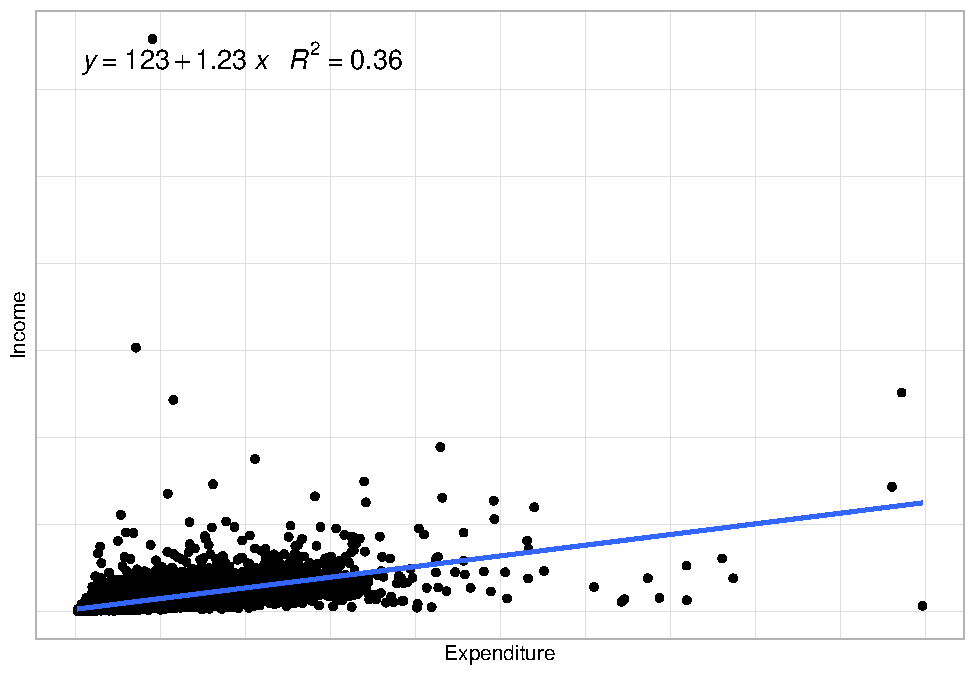
\includegraphics{06-Regresión_files/figure-latex/plot1-1.pdf}

Si bien, existen unas observaciones por fuera de la nube de punto, el comportamiento general de la relación ingresos vs gastos mantiene una tendencia lineal.

Una vez hecho el análisis gráfico de las variables a utilizar en los modelos a trabajar, se realizará primero un ajuste del modelo con los datos poblacionales y con esto poder analizar qué tan bueno serán los ajustes que se realizarán posteriormente. A continuación, se muestra el ajuste del modelo con los datos poblacionales:

\begin{Shaded}
\begin{Highlighting}[]
\NormalTok{fit }\OtherTok{\textless{}{-}} \FunctionTok{lm}\NormalTok{(Income }\SpecialCharTok{\textasciitilde{}}\NormalTok{ Expenditure, }\AttributeTok{data =}\NormalTok{ BigCity)}
\end{Highlighting}
\end{Shaded}

Ahora bien, para observar los parámetros poblacionales del modelo se utilizará la función \texttt{modelsummary} de la librería \texttt{modelsummary} de la siguiente manera:

\begin{longtable}[]{@{}lc@{}}
\caption{\label{tab:unnamed-chunk-4}Modelo BigCity}\tabularnewline
\toprule()
& Pob \\
\midrule()
\endfirsthead
\toprule()
& Pob \\
\midrule()
\endhead
(Intercept) & 123.337 \\
Expenditure & 1.229 \\
Num.Obs. & 150266 \\
R2 & 0.359 \\
R2 Adj. & 0.359 \\
RMSE & 461.74 \\
\bottomrule()
\end{longtable}

De la anterior salida se puede observar que, el intercepto es igual a 123.337 y el parámetro \(\beta_{1}\) asociado al gasto es 1.229. La demás información relacionada a esta salida se analizará más adelante.

Una vez revisada la información poblacional, se utilizará la información obtenida de la muestra para estimar los parámetros y con ello analizar qué tan buenas son las estimaciones. A continuación, se presenta una sintaxis similar a la anterior que permite construir el scatterplot pero para los datos de la muestra.

\begin{Shaded}
\begin{Highlighting}[]
\NormalTok{plot\_sin }\OtherTok{\textless{}{-}} \FunctionTok{ggplot}\NormalTok{(}\AttributeTok{data =}\NormalTok{ encuesta,}
            \FunctionTok{aes}\NormalTok{(}\AttributeTok{x =}\NormalTok{ Expenditure, }\AttributeTok{y =}\NormalTok{ Income)) }\SpecialCharTok{+}
            \FunctionTok{geom\_point}\NormalTok{() }\SpecialCharTok{+}
            \FunctionTok{geom\_smooth}\NormalTok{(}\AttributeTok{method =} \StringTok{"lm"}\NormalTok{,}
            \AttributeTok{se =} \ConstantTok{FALSE}\NormalTok{, }\AttributeTok{formula =}\NormalTok{ y }\SpecialCharTok{\textasciitilde{}}\NormalTok{ x) }\SpecialCharTok{+} \FunctionTok{theme\_cepal}\NormalTok{()}

\NormalTok{plot\_sin }\SpecialCharTok{+} \FunctionTok{stat\_poly\_eq}\NormalTok{(}\AttributeTok{formula =}\NormalTok{ y}\SpecialCharTok{\textasciitilde{}}\NormalTok{x, }\FunctionTok{aes}\NormalTok{(}\AttributeTok{label =} \FunctionTok{paste}\NormalTok{(..eq.label..,}
\NormalTok{     ..rr.label.., }\AttributeTok{sep =} \StringTok{"\textasciitilde{}\textasciitilde{}\textasciitilde{}"}\NormalTok{), }\AttributeTok{size =} \DecValTok{5}\NormalTok{), }\AttributeTok{parse =} \ConstantTok{TRUE}\NormalTok{)}
\end{Highlighting}
\end{Shaded}

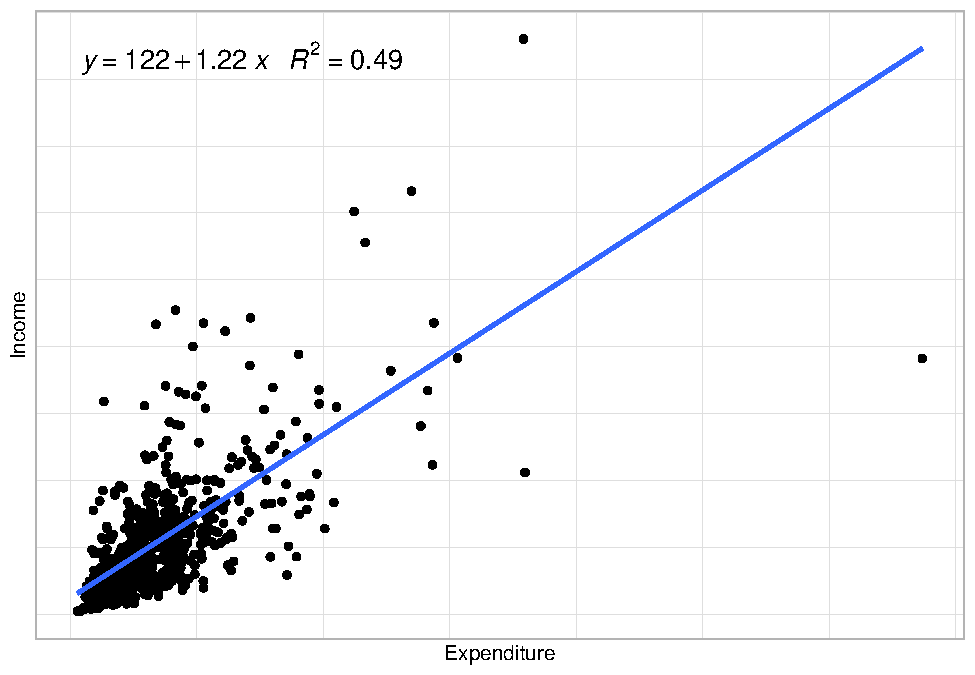
\includegraphics{06-Regresión_files/figure-latex/plot2-1.pdf}

Como se puede observar, los datos de la muestra tienen una tendencia lineal aunque un poco dispersa a medida que crecen los gastos en las familias.

Una vez hecho los análisis gráficos se procede a ajustar los modelos de regresión lineal. A modo de comparar el efecto que tiene hacer un correcto uso de los factores de expansión del diseño, primero, se ajustará un modelo sin tener encuesta dichos factores como se muestra a continuación:

\begin{Shaded}
\begin{Highlighting}[]
\NormalTok{fit\_sinP }\OtherTok{\textless{}{-}} \FunctionTok{lm}\NormalTok{(Income }\SpecialCharTok{\textasciitilde{}}\NormalTok{ Expenditure, }\AttributeTok{data =}\NormalTok{ encuesta)}
\NormalTok{fit\_sinP}
\end{Highlighting}
\end{Shaded}

\begin{verbatim}
## 
## Call:
## lm(formula = Income ~ Expenditure, data = encuesta)
## 
## Coefficients:
## (Intercept)  Expenditure  
##      121.52         1.22
\end{verbatim}

\begin{Shaded}
\begin{Highlighting}[]
\FunctionTok{stargazer}\NormalTok{(fit\_sinP, }\AttributeTok{header =} \ConstantTok{FALSE}\NormalTok{,}
          \AttributeTok{title =} \StringTok{"Modelo sin factores de expansion"}\NormalTok{, }
          \AttributeTok{style =} \StringTok{"ajps"}\NormalTok{)}
\end{Highlighting}
\end{Shaded}

\begin{verbatim}
## 
## \begin{table}[!htbp] \centering 
##   \caption{Modelo sin factores de expansion} 
##   \label{} 
## \begin{tabular}{@{\extracolsep{5pt}}lc} 
## \\[-1.8ex]\hline \\[-1.8ex] 
## \\[-1.8ex] & \textbf{Income} \\ 
## \hline \\[-1.8ex] 
##  Expenditure & 1.220$^{***}$ \\ 
##   & (0.025) \\ 
##   Constant & 121.500$^{***}$ \\ 
##   & (11.410) \\ 
##  N & 2605 \\ 
## R-squared & 0.487 \\ 
## Adj. R-squared & 0.487 \\ 
## Residual Std. Error & 345.000 (df = 2603) \\ 
## F Statistic & 2473.000$^{***}$ (df = 1; 2603) \\ 
## \hline \\[-1.8ex] 
## \multicolumn{2}{l}{$^{***}$p $<$ .01; $^{**}$p $<$ .05; $^{*}$p $<$ .1} \\ 
## \end{tabular} 
## \end{table}
\end{verbatim}

Para el modelo ajustado sin factores de expansión, el \(\hat{\beta}_{0}\) es 121.52 y el \(\hat{\beta}_{1}\) asociado a la variable gastos es 1.22.

Ahora, haciendo un Scatterplot con los datos encuesta pero utilizando los factores de expansión del diseño se debe agregar \texttt{mapping\ =\ aes(weight\ =\ wk)} en la función \texttt{geom\_smooth}como sigue:

\begin{Shaded}
\begin{Highlighting}[]
\NormalTok{plot\_Ponde }\OtherTok{\textless{}{-}} \FunctionTok{ggplot}\NormalTok{(}\AttributeTok{data =}\NormalTok{ encuesta,}
                     \FunctionTok{aes}\NormalTok{(}\AttributeTok{x =}\NormalTok{ Expenditure, }\AttributeTok{y =}\NormalTok{ Income)) }\SpecialCharTok{+} 
                     \FunctionTok{geom\_point}\NormalTok{(}\FunctionTok{aes}\NormalTok{(}\AttributeTok{size =}\NormalTok{ wk)) }\SpecialCharTok{+}
                     \FunctionTok{geom\_smooth}\NormalTok{(}\AttributeTok{method =} \StringTok{"lm"}\NormalTok{, }\AttributeTok{se =} \ConstantTok{FALSE}\NormalTok{, }\AttributeTok{formula =}\NormalTok{ y }\SpecialCharTok{\textasciitilde{}}\NormalTok{ x,                      }\AttributeTok{mapping =} \FunctionTok{aes}\NormalTok{(}\AttributeTok{weight =}\NormalTok{ wk)) }\SpecialCharTok{+} \FunctionTok{theme\_cepal}\NormalTok{()}

\NormalTok{plot\_Ponde }\SpecialCharTok{+} \FunctionTok{stat\_poly\_eq}\NormalTok{(}\AttributeTok{formula =}\NormalTok{ y}\SpecialCharTok{\textasciitilde{}}\NormalTok{x, }\FunctionTok{aes}\NormalTok{(}\AttributeTok{weight =}\NormalTok{ wk, }
\AttributeTok{label =} \FunctionTok{paste}\NormalTok{(..eq.label..,..rr.label.., }\AttributeTok{sep =} \StringTok{"\textasciitilde{}\textasciitilde{}\textasciitilde{}"}\NormalTok{)), }\AttributeTok{parse =} \ConstantTok{TRUE}\NormalTok{,}\AttributeTok{size =} \DecValTok{5}\NormalTok{)}
\end{Highlighting}
\end{Shaded}

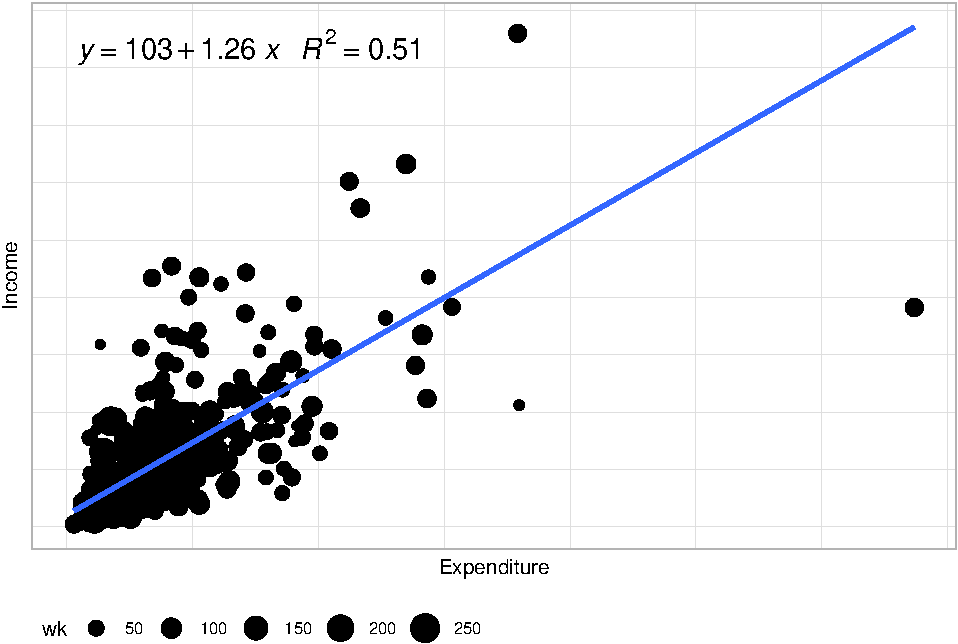
\includegraphics{06-Regresión_files/figure-latex/plot3-1.pdf}

En este sentido, para ajustar modelos teniendo en cuenta los factores de expansión existen 2 formas, la primera es usando la función \texttt{lm} y la segunda es usando la función \texttt{svyglm} de la librería \texttt{survey}. A continuación. se ajusta el modelo usando la función \texttt{lm}:

\begin{Shaded}
\begin{Highlighting}[]
\NormalTok{fit\_Ponde }\OtherTok{\textless{}{-}} \FunctionTok{lm}\NormalTok{(Income }\SpecialCharTok{\textasciitilde{}}\NormalTok{ Expenditure, }\AttributeTok{data =}\NormalTok{ encuesta, }\AttributeTok{weights =}\NormalTok{ wk)}
\NormalTok{fit\_Ponde}
\end{Highlighting}
\end{Shaded}

\begin{verbatim}
## 
## Call:
## lm(formula = Income ~ Expenditure, data = encuesta, weights = wk)
## 
## Coefficients:
## (Intercept)  Expenditure  
##      103.14         1.26
\end{verbatim}

\begin{Shaded}
\begin{Highlighting}[]
\FunctionTok{stargazer}\NormalTok{(fit\_Ponde, }\AttributeTok{header =} \ConstantTok{FALSE}\NormalTok{,}
          \AttributeTok{title =} \StringTok{"Modelo encuesta ponderada"}\NormalTok{, }
          \AttributeTok{style =} \StringTok{"ajps"}\NormalTok{)}
\end{Highlighting}
\end{Shaded}

\begin{verbatim}
## 
## \begin{table}[!htbp] \centering 
##   \caption{Modelo encuesta ponderada} 
##   \label{} 
## \begin{tabular}{@{\extracolsep{5pt}}lc} 
## \\[-1.8ex]\hline \\[-1.8ex] 
## \\[-1.8ex] & \textbf{Income} \\ 
## \hline \\[-1.8ex] 
##  Expenditure & 1.263$^{***}$ \\ 
##   & (0.024) \\ 
##   Constant & 103.100$^{***}$ \\ 
##   & (11.260) \\ 
##  N & 2605 \\ 
## R-squared & 0.509 \\ 
## Adj. R-squared & 0.509 \\ 
## Residual Std. Error & 2627.000 (df = 2603) \\ 
## F Statistic & 2703.000$^{***}$ (df = 1; 2603) \\ 
## \hline \\[-1.8ex] 
## \multicolumn{2}{l}{$^{***}$p $<$ .01; $^{**}$p $<$ .05; $^{*}$p $<$ .1} \\ 
## \end{tabular} 
## \end{table}
\end{verbatim}

Para el modelo ajustado con factores de expansión usando la función \texttt{lm}, el \(\hat{\beta}_{0}\) es 103.14 y el \(\hat{\beta}_{1}\) asociado a la variable gastos es 1.26. Ahora, haciendo el mismo ajuste pero usando la función \texttt{svyglm}:

\begin{Shaded}
\begin{Highlighting}[]
\NormalTok{fit\_svy }\OtherTok{\textless{}{-}} \FunctionTok{svyglm}\NormalTok{(Income }\SpecialCharTok{\textasciitilde{}}\NormalTok{ Expenditure, }
                  \AttributeTok{design =}\NormalTok{ diseno, }\AttributeTok{family=}\NormalTok{stats}\SpecialCharTok{::}\FunctionTok{gaussian}\NormalTok{())}
\NormalTok{fit\_svy}
\end{Highlighting}
\end{Shaded}

\begin{verbatim}
## Stratified 1 - level Cluster Sampling design (with replacement)
## With (238) clusters.
## Called via srvyr
## Sampling variables:
##  - ids: PSU
##  - strata: Stratum
##  - weights: wk
## 
## Call:  svyglm(formula = Income ~ Expenditure, design = diseno, family = stats::gaussian())
## 
## Coefficients:
## (Intercept)  Expenditure  
##      103.14         1.26  
## 
## Degrees of Freedom: 2604 Total (i.e. Null);  118 Residual
## Null Deviance:       6.35e+08 
## Residual Deviance: 3.11e+08  AIC: 38300
\end{verbatim}

Obteniendo estimaciones para el \(\hat{\beta}_{0}\) es 103.14 y el \(\hat{\beta}_{1}\) asociado a la variable gastos es 1.26. Siendo exactamente las mismas que con la función \texttt{lm} ya que, como se definió en los argumentos de la función, la función de enlace es Gausiana.

Por último y a modo de resumen se muestra un gráfico donde se encuentran depositados todos los modelos estimados anteriormente y así poder comparar de manera gráfica su ajuste:

\begin{Shaded}
\begin{Highlighting}[]
\NormalTok{df\_model }\OtherTok{\textless{}{-}} \FunctionTok{data.frame}\NormalTok{(}
  \AttributeTok{intercept =} \FunctionTok{c}\NormalTok{(}\FunctionTok{coefficients}\NormalTok{(fit)[}\DecValTok{1}\NormalTok{],}
               \FunctionTok{coefficients}\NormalTok{(fit\_sinP)[}\DecValTok{1}\NormalTok{], }
               \FunctionTok{coefficients}\NormalTok{(fit\_Ponde)[}\DecValTok{1}\NormalTok{],}
               \FunctionTok{coefficients}\NormalTok{(fit\_svy)[}\DecValTok{1}\NormalTok{]), }
  \AttributeTok{slope =} \FunctionTok{c}\NormalTok{(}\FunctionTok{coefficients}\NormalTok{(fit)[}\DecValTok{2}\NormalTok{],}
               \FunctionTok{coefficients}\NormalTok{(fit\_sinP)[}\DecValTok{2}\NormalTok{], }
               \FunctionTok{coefficients}\NormalTok{(fit\_Ponde)[}\DecValTok{2}\NormalTok{],}
               \FunctionTok{coefficients}\NormalTok{(fit\_svy)[}\DecValTok{2}\NormalTok{]),}
  \AttributeTok{Modelo =} \FunctionTok{c}\NormalTok{(}\StringTok{"Población"}\NormalTok{, }\StringTok{"Sin ponderar"}\NormalTok{, }
             \StringTok{"Ponderado(lm)"}\NormalTok{, }\StringTok{"Ponderado(svyglm)"}\NormalTok{))}
\NormalTok{plot\_BigCity }\SpecialCharTok{+}  \FunctionTok{geom\_abline}\NormalTok{( }\AttributeTok{data =}\NormalTok{ df\_model,}
    \AttributeTok{mapping =} \FunctionTok{aes}\NormalTok{( }\AttributeTok{slope =}\NormalTok{ slope,}
      \AttributeTok{intercept =}\NormalTok{ intercept, }\AttributeTok{linetype =}\NormalTok{ Modelo,}
      \AttributeTok{color =}\NormalTok{ Modelo ), }\AttributeTok{size =} \DecValTok{2}
\NormalTok{  )}
\end{Highlighting}
\end{Shaded}

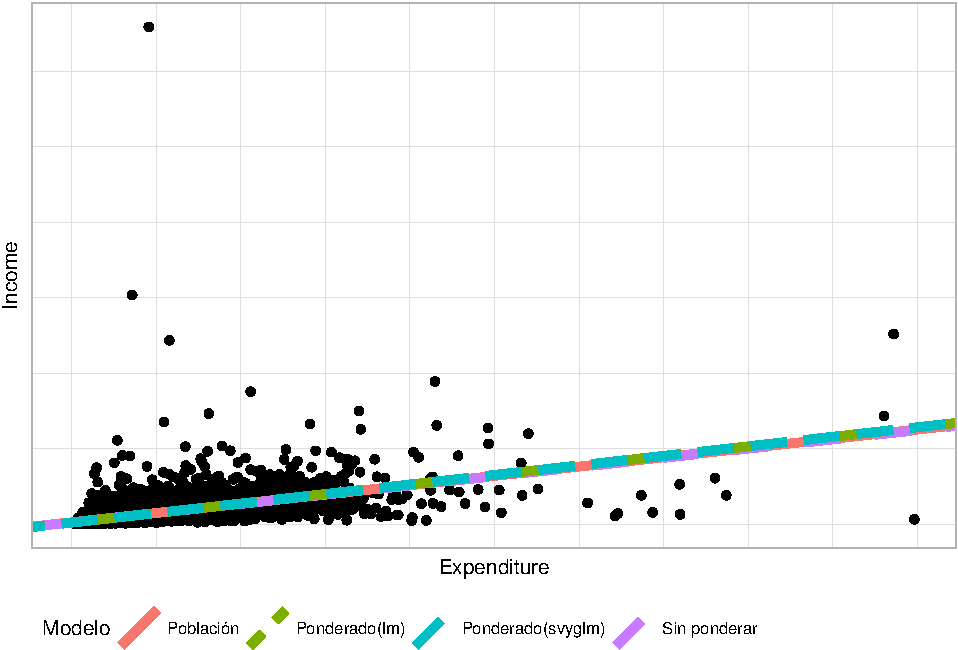
\includegraphics{06-Regresión_files/figure-latex/plot4-1.pdf}

\hypertarget{diagnuxf3stico-del-modelo}{%
\section{Diagnóstico del modelo}\label{diagnuxf3stico-del-modelo}}

En el análisis de las encuestas de hogares cuando se ajusten modelo estadístico es importante realizar verificaciones de calidad y con esto tener certezas de las conclusiones que se obtienen. La mayoría de textos académicos dan un panorama bastante detallado de los supuestos y consideraciones que se deben tener en cuenta para tener un modelo correctamente definido. A continuación, se enlistan algunas de ellas \emph{(Tellez, 2016)}

\begin{itemize}
\tightlist
\item
  Determinar si el modelo proporciona un adecuado ajuste a los datos.
\item
  Examinar si los errores están normalmente distribuidos.
\item
  Examinar si los errores tienen varianza constante.
\item
  Verificar si los errores se pueden asumir no correlacionados.
\item
  Determinar si alguno de los datos tiene valores con un efecto inusualmente grande sobre el modelo de regresión estimado, estos se conocen
  como datos influyentes.
\item
  Determinar si algún punto no sigue la tendencia de la mayoría de los
  datos cuando se toma en cuenta el modelo, estos puntos se conocen como outliers.
\end{itemize}

En este capítulo se abordarán alguno de los supuestos que se deben tener en cuenta al momento de ajustar un modelo de regresión lineal.

\emph{Estimación del \(R^{2}\) y \(R_{adj}^{2}\)}

Una medida del ajuste del modelo de regresión es el coeficiente de determinación o coeficiente de correlación múltiple (\(R^{2})\)). Dicho parámetro estima la proporción de la varianza de la población explicada por la regresión y oscila entre 0 y 1. Entre más cercano esté de uno significa que mayor variabilidad explica y lo contrario ocurrirá si está cerca de cero. Lo anterior, en ocasiones es muy ambigüo puesto que por ejemplo, los físicos pueden obtienen \(R^{2}\) altísimos (mayores a 0.98--0.99) mientras que los químicos obtienen \(R^{2}\) superiores a 0.90. Sin embargo, los científicos sociales y demás que trabajen con poblaciones humanas encontrarán que su mejor modelo de regresión a menudo explicará solo entre el 20 \% y el 40 \% de la variación en la variable dependiente (\emph{Heringa}). A continuación, se presenta como se calcula este coeficiente:

\[
R^{2} =  1-\frac{SSE}{SST}
\]

Donde, SST es la suma de cuadrados totales y SSE es la suma de cuadrados del error. El estimador de este parámetro usando muestras complejas está dado por:

\[
R_{\omega}^{2} = 1-\frac{WSSE}{WSST}
\]

Donde, WSST es la variabilidad total estimada y WSSE es la suma de cuadrados estimada y se define como:

\[
\hat{WSSE_{\omega}}  =  \sum_{h}^{H}\sum_{\alpha}^{a_{h}}\sum_{i=1}^{n_{h\alpha}}\omega_{h\alpha i}\left(y_{h\alpha i}-x_{h\alpha i}\hat{\beta}\right)^{2}
\]

Por último, \(R_{adj}^{2}\) se estima:

\[
R_{adj}^{2}  =  1-\frac{\left(n-1\right)}{\left(n-p\right)}R_{\omega}^{2}
\]

Para continuar con los modelos ajustados en la sección anterior, se procede a estimar los \(R^{2}\) utilizando \texttt{R}. Inicialmente, se procede a estimar los parámetros del modelo utilizando la función \texttt{svyglm} de \texttt{survey} como se mostró anteriormente y también, se ajusta un modelo solo con el intercepto para obtener la estimación de la SST:

\begin{Shaded}
\begin{Highlighting}[]
\NormalTok{fit\_svy }\OtherTok{\textless{}{-}} \FunctionTok{svyglm}\NormalTok{(Income }\SpecialCharTok{\textasciitilde{}}\NormalTok{ Expenditure, }
                  \AttributeTok{design =}\NormalTok{ diseno)}

\NormalTok{modNul }\OtherTok{\textless{}{-}} \FunctionTok{svyglm}\NormalTok{(Income }\SpecialCharTok{\textasciitilde{}} \DecValTok{1}\NormalTok{, }\AttributeTok{design =}\NormalTok{ diseno)}

\NormalTok{s1 }\OtherTok{\textless{}{-}} \FunctionTok{summary}\NormalTok{(fit\_svy)}
\NormalTok{s0 }\OtherTok{\textless{}{-}}\FunctionTok{summary}\NormalTok{(modNul)}

\NormalTok{WSST}\OtherTok{\textless{}{-}}\NormalTok{ s0}\SpecialCharTok{$}\NormalTok{dispersion}
\NormalTok{WSSE}\OtherTok{\textless{}{-}}\NormalTok{ s1}\SpecialCharTok{$}\NormalTok{dispersion}
\end{Highlighting}
\end{Shaded}

Por tanto, la estimación del \(R^{2}\) es:

\begin{Shaded}
\begin{Highlighting}[]
\NormalTok{R2 }\OtherTok{=} \DecValTok{1}\SpecialCharTok{{-}}\NormalTok{ WSSE}\SpecialCharTok{/}\NormalTok{WSST}
\NormalTok{R2}
\end{Highlighting}
\end{Shaded}

\begin{verbatim}
##      variance    SE
## [1,]    0.509 19005
\end{verbatim}

y, para estimar el \(R_{adj}^{2}\) se requiere definir el diseño muestral pero incluyendo los q-weigthed \textbf{(Pffeferman, 2011)}. A continuación, se muestra los pasos para encontrar los q-weigthed:

\begin{itemize}
\tightlist
\item
  Ajustar un modelo de regresión a los pesos finales de la encuesta utilizando las variables predictoras en el modelo de regresión de interés.
\end{itemize}

\begin{Shaded}
\begin{Highlighting}[]
\NormalTok{fit\_Nul }\OtherTok{\textless{}{-}} \FunctionTok{lm}\NormalTok{(wk }\SpecialCharTok{\textasciitilde{}} \DecValTok{1}\NormalTok{, }\AttributeTok{data =}\NormalTok{ encuesta)}
\end{Highlighting}
\end{Shaded}

\begin{itemize}
\tightlist
\item
  Obtener las predicciones de los pesos de la encuesta para cada caso como una función de las variables predictoras en el conjunto de datos
\end{itemize}

\begin{Shaded}
\begin{Highlighting}[]
\NormalTok{qw }\OtherTok{\textless{}{-}} \FunctionTok{predict}\NormalTok{(fit\_Nul)}
\end{Highlighting}
\end{Shaded}

\begin{itemize}
\tightlist
\item
  Dividir los pesos finales de la encuesta por los valores predichos en el paso anterior:
\end{itemize}

\begin{Shaded}
\begin{Highlighting}[]
\NormalTok{encuesta }\SpecialCharTok{\%\textless{}\textgreater{}\%} \FunctionTok{mutate}\NormalTok{(}\AttributeTok{wk1 =}\NormalTok{ wk}\SpecialCharTok{/}\NormalTok{qw)}
\end{Highlighting}
\end{Shaded}

\begin{itemize}
\tightlist
\item
  Usar los nuevos pesos obtenidos para el ajuste de los modelos de regresión:
\end{itemize}

\begin{Shaded}
\begin{Highlighting}[]
\NormalTok{diseno\_qwgt }\OtherTok{\textless{}{-}}\NormalTok{ encuesta }\SpecialCharTok{\%\textgreater{}\%}
  \FunctionTok{as\_survey\_design}\NormalTok{(}
    \AttributeTok{strata =}\NormalTok{ Stratum,}
    \AttributeTok{ids =}\NormalTok{ PSU,}
    \AttributeTok{weights =}\NormalTok{ wk1,}
    \AttributeTok{nest =}\NormalTok{ T)}
\end{Highlighting}
\end{Shaded}

Ahora bien, una vez definido el diseño muestral con los nuevos pesos q-weigthed, se procede a calcular el \(R_{adj}^{2}\) como sigue:

\begin{Shaded}
\begin{Highlighting}[]
\NormalTok{n }\OtherTok{=} \FunctionTok{sum}\NormalTok{(diseno\_qwgt}\SpecialCharTok{$}\NormalTok{variables}\SpecialCharTok{$}\NormalTok{wk)}
\NormalTok{p}\OtherTok{\textless{}{-}} \DecValTok{2}
\NormalTok{R2Adj }\OtherTok{=} \DecValTok{1}\SpecialCharTok{{-}}\NormalTok{( ( (n}\DecValTok{{-}1}\NormalTok{)}\SpecialCharTok{/}\NormalTok{(n}\SpecialCharTok{{-}}\NormalTok{p) )}\SpecialCharTok{*}\NormalTok{R2 )}
\NormalTok{R2Adj             }
\end{Highlighting}
\end{Shaded}

\begin{verbatim}
##      variance    SE
## [1,]    0.491 19005
\end{verbatim}

Como se puede observar, el \(R_{adj}^{2}\) es un poco más bajo que el \(R^{2}\) y cercanos al 50\% que como se comentó anteriormente, dependiendo del contexto del problema se podrá concluir si es grande o pequeño.

Después de realizar la comparación entre las diferentes formas de estimar los coeficientes del modelo se opta por la metodología consolidadas en \texttt{svyglm}:

\begin{Shaded}
\begin{Highlighting}[]
\NormalTok{diseno\_qwgt }\SpecialCharTok{\%\textless{}\textgreater{}\%} \FunctionTok{mutate}\NormalTok{(}\AttributeTok{Age2 =}\NormalTok{ Age}\SpecialCharTok{\^{}}\DecValTok{2}\NormalTok{) }
\NormalTok{mod\_svy }\OtherTok{\textless{}{-}} \FunctionTok{svyglm}\NormalTok{( Income }\SpecialCharTok{\textasciitilde{}}\NormalTok{ Expenditure }\SpecialCharTok{+}\NormalTok{ Zone }\SpecialCharTok{+}\NormalTok{ Sex }\SpecialCharTok{+}\NormalTok{ Age2 ,}
                       \AttributeTok{design =}\NormalTok{ diseno\_qwgt)}
\NormalTok{s1 }\OtherTok{\textless{}{-}} \FunctionTok{summary}\NormalTok{(mod\_svy)}
\NormalTok{s0 }\OtherTok{\textless{}{-}} \FunctionTok{summary}\NormalTok{(modNul)}

\NormalTok{mod\_svy}
\end{Highlighting}
\end{Shaded}

Stratified 1 - level Cluster Sampling design (with replacement)
With (238) clusters.
Called via srvyr
Sampling variables:
- ids: PSU
- strata: Stratum
- weights: wk1

Call: svyglm(formula = Income \textasciitilde{} Expenditure + Zone + Sex + Age2, design = diseno\_qwgt)

Coefficients:
(Intercept) Expenditure ZoneUrban SexMale Age2\\
62.18419 1.22548 63.46000 21.73256 0.00852

Degrees of Freedom: 2604 Total (i.e.~Null); 115 Residual
Null Deviance: 6.35e+08
Residual Deviance: 3.08e+08 AIC: 38300

\begin{Shaded}
\begin{Highlighting}[]
\FunctionTok{stargazer}\NormalTok{(mod\_svy, }\AttributeTok{header =} \ConstantTok{FALSE}\NormalTok{,}\AttributeTok{single.row =}\NormalTok{ T,}
           \AttributeTok{title =} \StringTok{"Modelo propuesto"}\NormalTok{, }
           \AttributeTok{style =} \StringTok{"ajps"}\NormalTok{,  }\AttributeTok{omit.stat=}\FunctionTok{c}\NormalTok{(}\StringTok{"bic"}\NormalTok{, }\StringTok{"ll"}\NormalTok{))}
\end{Highlighting}
\end{Shaded}

\begin{table}[!htbp] \centering 
  \caption{Modelo propuesto} 
  \label{} 
\begin{tabular}{@{\extracolsep{5pt}}lc} 
\\[-1.8ex]\hline \\[-1.8ex] 
\\[-1.8ex] & \textbf{Income} \\ 
\hline \\[-1.8ex] 
 Expenditure & 1.225$^{***}$ (0.198) \\ 
  ZoneUrban & 63.460 (40.090) \\ 
  SexMale & 21.730 (15.780) \\ 
  Age2 & 0.009 (0.006) \\ 
  Constant & 62.180 (62.990) \\ 
 N & 2605 \\ 
AIC & 38259.000 \\ 
\hline \\[-1.8ex] 
\multicolumn{2}{l}{$^{***}$p $<$ .01; $^{**}$p $<$ .05; $^{*}$p $<$ .1} \\ 
\end{tabular} 
\end{table}

\emph{Diagnósticos de los residuales}

En el diagnóstico de los modelos es crucial el análisis de los residuales. Estos análisis proporcionan, bajo el supuesto que el modelo ajustado es
adecuado, una estimación de los errores. Por tanto, un estudio cuidadoso
de los residuales deberá ayudar al investigador a concluir si el procedimiento de ajuste no ha violado los supuestos o si, por el contrario, uno o varios de los supuestos no se verifican y hay necesidad de revisar el procedimiento de ajuste.

Para realizar el análisis de los residuales, en primera instancia, se definen los residuales de Pearson como sigue \emph{(Heeringa)}

\[
r_{p_{i}}  =  \left(y_{i}-\mu_{i}\left(\hat{\beta}_{\omega}\right)\right)\sqrt{\frac{\omega_{i}}{V\left(\hat{\mu}_{i}\right)}}
\]
Donde, \(\mu_{i}\) es el valor esperado de \(y_{i}\), \(w_{i}\) es la ponderación de la encuesta para el i-ésimo individuo del diseño muestral complejo, Por último, \(V(\mu_{i})\) es la función de varianza del resultado.

Otra definición que se debe tener en consideración para el análisis de los residuales es el de la matriz hat, la cual se estima como:

\[
H  =  W^{1/2}X\left(X'WX\right)^{-1}X'W^{1/2}
\]
donde,

\[
W  =  diag\left\{ \frac{\omega_{1}}{V\left(\mu_{1}\right)\left[g'\left(\mu_{1}\right)\right]^{2}},...,\frac{\omega_{n}}{V\left(\mu_{n}\right)\left[g'\left(\mu_{n}\right)\right]^{2}}\right\} 
\]
\(W\) es una matriz diagonal de \(n\times n\) y \(g()\) es la función de enlace del modelo lineal generalizado.

Otras técnicas utilizadas también para el análisis de los modelos consisten en el análisis de observaciones influyentes. Una observación se denomina influyente si al removerlo de la nube de puntos este causa un cambio grande en el ajuste del modelo. Una observación importante para resaltar es que un punto influyente podría o no ser un dato atípico. Para detectar observaciones influyentes es necesario tener claro qué tipo de influencia se quiere detectar. Lo anterior puesto que, por ejemplo, una observación puede ser influyente sobre la estimación de los parámetros, pero no para la estimación de la varianza del error. A continuación, se presentan las distintas técnicas estadísticas para la detección de datos influyentes:

\emph{Distancia de Cook's}: Diagnostica si la i-ésima observación es influyente
en la estimación del modelo, por estar lejos del centro de masa de los
datos. Se calcula de la siguiente manera:

\[
c_{i}=\frac{w_{i}^{*}w_{i}e_{i}^{2}}{p\phi V\left(\hat{\mu}_{i}\right)\left(1-h_{ii}\right)^{2}}\boldsymbol{x}_{i}^{t}\left[\widehat{Var}\left(U_{w}\left(\hat{\boldsymbol{B}}_{w}\right)\right)\right]^{-1}\boldsymbol{x}_{i}
\]

donde,

\begin{itemize}
\tightlist
\item
  \(w_i^* =\) Pesos de la encuesta.
\item
  \(w_i\) Elementos por fuera de la diagonal de la matriz hat
\item
  \(e_i=\) residuales
\item
  \(p=\) número de parámetros del Modelo de regresión.
\item
  \(\phi =\) parámetro de dispersión en el glm
\item
  \(\widehat{Var}\left(U_{w}\left(\hat{\boldsymbol{B}}_{w}\right)\right) =\) estimación de varianza linealizada de la ecuación de puntuación, que se utiliza para pseudo MLE en modelos lineales generalizados ajustados a datos de encuestas de muestras complejas.
\end{itemize}

Luego del cálculo de la distancia de Cook's para las observaciones de la muestra, se procede a calcular el siguiente estadístico de prueba para evaluar la importancia de la estadística:

\[
\frac{\left(df-p+1\right)\times c_{i}}{df} \doteq F_{\left(p,df-p\right)}
\]

donde \(df=\) grados de liberta basados en el diseño. Por otro lado, la literatura como \emph{Tellez (2016)}, \emph{Heeringa} considera a las observaciones influyentes cuando \(c_{i}\) sean mayores a 2 o 3.

\emph{\(D_fBeta_{(i)}\)}: Este estadístico mide el cambio en la estimación
del vector de coeficientes de regresión cuando la i-ésima observación
es eliminada. Se evalúa con la siguiente expresión:

\[
D_fBeta_{(i)} = \hat{B}-\hat{B}_{\left(i\right)}=\frac{\boldsymbol{A}^{-1}\boldsymbol{X}_{\left(i\right)}^{t}\hat{e}_{i}w_{i}}{1-h_{ii}}
\]

Donde \(\boldsymbol{A} =\boldsymbol{X}^{t}\boldsymbol{WX}\) \(\hat{B}_{(i)}\) es el vector de parámetros estimados una vez se ha eliminado la
i-ésima observación, \(h_{ii}\) es el correspondiente elemento de la diagonal de \emph{H} y \(\hat{e}_i\) es el residual de la i-ésima observación.

Otra forma de reescribir este estadístico en términos de la matriz \(H\) es:

\[
D_fBetas_{\left(i\right)}=\frac{{c_{ji}e_{i}}\big/{\left(1-h_{ii}\right)}}{\sqrt{v\left(\hat{B}_{j}\right)}}
\]

donde:

\begin{itemize}
\item
  \(c_{ji}=\) es el ji-estimo elemento de \(\boldsymbol{A}^{-1}w_{i}^{2}\boldsymbol{X}_{\left(i\right)}\boldsymbol{X}_{\left(i\right)}^{t}\boldsymbol{A}^{-1}\)
\item
  El estimador de \(v\left(\hat{B}_{j}\right)\) basado en el Modelo se obtiene como: \(v_{m}\left(\hat{B}_{j}\right)=\hat{\sigma}\sum_{i=1}^{n}c_{ji}^{2}\) con \(\hat{\sigma}=\sum_{i\in s}w_{i}e^2/ \left( \hat{N} - p \right)\) y \(\hat{N} = \sum_{i \in s}w_{i}\)
\item
  La i-ésima observación es influyente para \(B_j\) si \(\mid D_{f}Betas_{\left(i\right)j}\mid\geq\frac{z}{\sqrt{n}}\) con \(z=\) 2 o 3
\item
  Como alternativa puede usar \(t_{0.025,n-p}/\sqrt(n)\) donde \(t_{0.025,n-p}\) es el percentil \(97.5\)
\end{itemize}

\emph{Estadístico \(D_{f}Fits_{\left(i\right)}\)}: Este estadístico mide el cambio en el ajuste del modelo cuando se elimina el registro i-ésimo. Se calcula de la siguiente manera:

\[
D_{f}Fits_{\left(i\right)}= \frac{h_{ii}e_{i}\big/\left(1-h_{ii}\right)}{\sqrt{v\left(\hat{\beta}_{j}\right)}}
\]

Donde, \(\sqrt{v\left(\hat{\beta}_{j}\right)}\) puede ser aproximada por el diseño o el Modelo. La i-ésima observación se considera influyente en el ajuste del Modelo si
\(\mid DfFits\left(i\right)\mid\geq z\sqrt{\frac{p}{n}}\) con \(z =\) 2 o 3

Por otro lado, un análisis que es de vital importancia en el ajuste de modelos de regresión más específicamente en el análisis de residuales es el de varianza constante en los errores. La principal consecuencia de no tener en cuenta la violación de este supuesto es que los estimadores pierden eficiencia. Si el supuesto de varianza constante no se cumple, los estimadores siguen siendo insesgados y consistentes, pero dejan de ser eficientes, es decir, dejan de ser los mejores en cuanto a que ya no tienen la menor varianza entre todos los estimadores insesgados. Como consecuencia de lo anterior, los intervalos de confianza serán más amplios y las pruebas t y F darán resultados imprecisos \emph{(Tellez, 2016)}.

Una de las formas de analizar el supuesto de varianzas constantes en los errores es hacerlo de manera gráfica. Para ello, se grafica los residuos del modelo contra \(\hat{y}\) o los residuos del modelo contra \(X_{i}\). Si al realizar estos gráficos se logra evidenciar un patrón (funciones cuadráticas, cúbicas, logarítmicas, etc), se puede decir que la varianza de los errores no es constante.

Otro supuesto que se debe revisar en los errores al momento de realizar ajustes es la normalidad en lo errores. Una forma muy común para hacer dicha evaluación es realizar un gráfico cuantil-cuantil normal o QQplot. El QQplot es una gráfica de cuantiles para los residuos observados frente a los calculados a partir de una distribución normal teórica que tiene la misma media y varianza que la distribución de los residuos observados. Por lo tanto, una línea recta de 45° en este gráfico sugeriría que la normalidad es una suposición razonable para los errores aleatorios en el modelo.

A manera de ejemplificar los conceptos vistos, se van a utilizar los modelos previamente ajustados. En primero instancia, el análisis del modelo se centrará en los supuestos de normalidad y varianza constante en los errores. Primero, se realizará el análisis de la normalidad en los errores de manera gráfica como se muestra a continuación:

\begin{Shaded}
\begin{Highlighting}[]
\FunctionTok{par}\NormalTok{(}\AttributeTok{mfrow =} \FunctionTok{c}\NormalTok{(}\DecValTok{2}\NormalTok{,}\DecValTok{2}\NormalTok{))}
\FunctionTok{plot}\NormalTok{(mod\_svy)}
\end{Highlighting}
\end{Shaded}

\includegraphics{06-Regresión_files/figure-latex/unnamed-chunk-12-1.pdf}

Como se puedo observar en el QQplot, hay evidencia gráfica de que los errores no se distribuyen según una distribución normal.

La librería \texttt{svydiags} está pensada en ayudar en el diagnostico de modelos de regresión lineal, siendo una extensión más para complementar el paquete \texttt{survey}. Con las librerías \texttt{svydiags} se extraen los residuales estandarizados como sigue:

\begin{Shaded}
\begin{Highlighting}[]
\FunctionTok{library}\NormalTok{(svydiags)}
\NormalTok{stdresids }\OtherTok{=} \FunctionTok{as.numeric}\NormalTok{(}\FunctionTok{svystdres}\NormalTok{(mod\_svy)}\SpecialCharTok{$}\NormalTok{stdresids)}
\NormalTok{diseno\_qwgt}\SpecialCharTok{$}\NormalTok{variables }\SpecialCharTok{\%\textless{}\textgreater{}\%} \FunctionTok{mutate}\NormalTok{(}\AttributeTok{stdresids =}\NormalTok{ stdresids)}
\end{Highlighting}
\end{Shaded}

Podemos hacer el análisis de normalidad también por medio del histograma de los residuales estandarizados como sigue:

\begin{Shaded}
\begin{Highlighting}[]
\FunctionTok{ggplot}\NormalTok{(}\AttributeTok{data =}\NormalTok{ diseno\_qwgt}\SpecialCharTok{$}\NormalTok{variables,}
       \FunctionTok{aes}\NormalTok{(}\AttributeTok{x =}\NormalTok{ stdresids)) }\SpecialCharTok{+}
  \FunctionTok{geom\_histogram}\NormalTok{(}\FunctionTok{aes}\NormalTok{(}\AttributeTok{y =}\NormalTok{ ..density..),}
                 \AttributeTok{colour =} \StringTok{"black"}\NormalTok{, }
                 \AttributeTok{fill =} \StringTok{"blue"}\NormalTok{, }\AttributeTok{alpha =} \FloatTok{0.3}\NormalTok{) }\SpecialCharTok{+}
  \FunctionTok{geom\_density}\NormalTok{(}\AttributeTok{size =} \DecValTok{2}\NormalTok{, }\AttributeTok{colour =} \StringTok{"blue"}\NormalTok{) }\SpecialCharTok{+}
  \FunctionTok{geom\_function}\NormalTok{(}\AttributeTok{fun =}\NormalTok{ dnorm, }\AttributeTok{colour =} \StringTok{"red"}\NormalTok{,}
                \AttributeTok{size =} \DecValTok{2}\NormalTok{) }\SpecialCharTok{+}
  \FunctionTok{theme\_cepal}\NormalTok{()}\SpecialCharTok{+}\FunctionTok{labs}\NormalTok{(}\AttributeTok{y =} \StringTok{""}\NormalTok{)}
\end{Highlighting}
\end{Shaded}

y como se puede observar gráficamente los errores no siguen una distribución normal.

Por otro lado, el otro análisis que se realiza de manera gráfica es el de varianzas constantes el cual se realizará a continuación:

Primero, agreguemos las predicciones a la base de datos para poder realizar las gráficas.

\begin{Shaded}
\begin{Highlighting}[]
\FunctionTok{library}\NormalTok{(patchwork)}
\NormalTok{diseno\_qwgt}\SpecialCharTok{$}\NormalTok{variables }\SpecialCharTok{\%\textless{}\textgreater{}\%} 
  \FunctionTok{mutate}\NormalTok{(}\AttributeTok{pred =} \FunctionTok{predict}\NormalTok{(mod\_svy))}
\NormalTok{g2 }\OtherTok{\textless{}{-}} \FunctionTok{ggplot}\NormalTok{(}\AttributeTok{data =}\NormalTok{ diseno\_qwgt}\SpecialCharTok{$}\NormalTok{variables,}
       \FunctionTok{aes}\NormalTok{(}\AttributeTok{x =}\NormalTok{ Expenditure, }\AttributeTok{y =}\NormalTok{ stdresids))}\SpecialCharTok{+}
  \FunctionTok{geom\_point}\NormalTok{() }\SpecialCharTok{+}
  \FunctionTok{geom\_hline}\NormalTok{(}\AttributeTok{yintercept =} \DecValTok{0}\NormalTok{) }\SpecialCharTok{+} \FunctionTok{theme\_cepal}\NormalTok{()}
\NormalTok{g3 }\OtherTok{\textless{}{-}} \FunctionTok{ggplot}\NormalTok{(}\AttributeTok{data =}\NormalTok{ diseno\_qwgt}\SpecialCharTok{$}\NormalTok{variables,}
       \FunctionTok{aes}\NormalTok{(}\AttributeTok{x =}\NormalTok{ Age2, }\AttributeTok{y =}\NormalTok{ stdresids))}\SpecialCharTok{+}
  \FunctionTok{geom\_point}\NormalTok{() }\SpecialCharTok{+}
  \FunctionTok{geom\_hline}\NormalTok{(}\AttributeTok{yintercept =} \DecValTok{0}\NormalTok{) }\SpecialCharTok{+} \FunctionTok{theme\_cepal}\NormalTok{()}
\end{Highlighting}
\end{Shaded}

\begin{Shaded}
\begin{Highlighting}[]
\NormalTok{g4 }\OtherTok{\textless{}{-}} \FunctionTok{ggplot}\NormalTok{(}\AttributeTok{data =}\NormalTok{ diseno\_qwgt}\SpecialCharTok{$}\NormalTok{variables,}
       \FunctionTok{aes}\NormalTok{(}\AttributeTok{x =}\NormalTok{ Zone, }\AttributeTok{y =}\NormalTok{ stdresids))}\SpecialCharTok{+}
  \FunctionTok{geom\_point}\NormalTok{() }\SpecialCharTok{+}
  \FunctionTok{geom\_hline}\NormalTok{(}\AttributeTok{yintercept =} \DecValTok{0}\NormalTok{) }\SpecialCharTok{+} \FunctionTok{theme\_cepal}\NormalTok{()}
\NormalTok{g5 }\OtherTok{\textless{}{-}} \FunctionTok{ggplot}\NormalTok{(}\AttributeTok{data =}\NormalTok{ diseno\_qwgt}\SpecialCharTok{$}\NormalTok{variables,}
       \FunctionTok{aes}\NormalTok{(}\AttributeTok{x =}\NormalTok{ Sex, }\AttributeTok{y =}\NormalTok{ stdresids))}\SpecialCharTok{+}
  \FunctionTok{geom\_point}\NormalTok{() }\SpecialCharTok{+}  \FunctionTok{geom\_hline}\NormalTok{(}\AttributeTok{yintercept =} \DecValTok{0}\NormalTok{) }\SpecialCharTok{+}
  \FunctionTok{theme\_cepal}\NormalTok{()}

\NormalTok{(g2}\SpecialCharTok{|}\NormalTok{g3)}\SpecialCharTok{/}\NormalTok{(g4}\SpecialCharTok{|}\NormalTok{g5)}
\end{Highlighting}
\end{Shaded}

Como se puede observar en las gráficas de gastos y edad, ambas muestran tendencias y no un comportamiento aleatorio. Por lo anterior, se puede decir que las varianzas no son constantes.

Otros de os análisis a realizar es revisar si existen datos influyentes en la base de datos. Para ejemplificar los conceptos definidos, se seguirán con los modelos ajustados en la sección anterior. Una vez ajustados estos modelos y verificados los supuestos, se procede a hacer el cálculo de la distancia de Cook's usando la función \texttt{svyCooksD}del paquete \texttt{svydiags} como sigue:

\begin{Shaded}
\begin{Highlighting}[]
\FunctionTok{library}\NormalTok{(svydiags) }
\NormalTok{d\_cook }\OtherTok{=} \FunctionTok{data.frame}\NormalTok{(}
   \AttributeTok{cook =} \FunctionTok{svyCooksD}\NormalTok{(mod\_svy), }
     \AttributeTok{id =} \DecValTok{1}\SpecialCharTok{:}\FunctionTok{length}\NormalTok{(}\FunctionTok{svyCooksD}\NormalTok{(mod\_svy)))}

\FunctionTok{table}\NormalTok{(d\_cook}\SpecialCharTok{$}\NormalTok{cook}\SpecialCharTok{\textgreater{}}\DecValTok{3}\NormalTok{)}


\FunctionTok{ggplot}\NormalTok{(d\_cook, }\FunctionTok{aes}\NormalTok{(}\AttributeTok{y =}\NormalTok{ cook, }\AttributeTok{x =}\NormalTok{ id)) }\SpecialCharTok{+}
  \FunctionTok{geom\_point}\NormalTok{() }\SpecialCharTok{+} 
  \FunctionTok{theme\_bw}\NormalTok{(}\DecValTok{20}\NormalTok{)}
\end{Highlighting}
\end{Shaded}

Como se puede observar, ninguna de las distancias de Cook's es mayor a 3 por lo que, podemos decir que no existen observaciones influyentes.

Ahora bien, se desea observar si hay observaciones influyentes pero utilizando \(D_{f}Betas_{\left(i\right)j}\) se realiza con la función \texttt{svydfbetas} como se muestra a continuación:

\begin{Shaded}
\begin{Highlighting}[]
\NormalTok{d\_dfbetas }\OtherTok{=} \FunctionTok{data.frame}\NormalTok{(}\FunctionTok{t}\NormalTok{(}\FunctionTok{svydfbetas}\NormalTok{(mod\_svy)}\SpecialCharTok{$}\NormalTok{Dfbetas))}
\FunctionTok{colnames}\NormalTok{(d\_dfbetas) }\OtherTok{\textless{}{-}} \FunctionTok{paste0}\NormalTok{(}\StringTok{"Beta\_"}\NormalTok{, }\DecValTok{1}\SpecialCharTok{:}\DecValTok{5}\NormalTok{)}
\NormalTok{d\_dfbetas }\SpecialCharTok{\%\textgreater{}\%} \FunctionTok{slice}\NormalTok{(}\DecValTok{1}\SpecialCharTok{:}\NormalTok{10L)}
\end{Highlighting}
\end{Shaded}

\begin{tabular}{r|r|r|r|r}
\hline
Beta\_1 & Beta\_2 & Beta\_3 & Beta\_4 & Beta\_5\\
\hline
0.0006 & -2e-04 & 0.0021 & -0.0045 & -0.0077\\
\hline
-0.0006 & -1e-04 & 0.0014 & 0.0026 & -0.0031\\
\hline
-0.0009 & -1e-04 & 0.0009 & 0.0022 & 0.0008\\
\hline
-0.0004 & -1e-04 & 0.0012 & -0.0031 & 0.0007\\
\hline
-0.0009 & 0e+00 & 0.0008 & 0.0021 & 0.0014\\
\hline
0.0009 & 6e-04 & -0.0036 & -0.0063 & 0.0098\\
\hline
0.0027 & 4e-04 & -0.0031 & -0.0076 & -0.0028\\
\hline
0.0011 & 3e-04 & -0.0028 & 0.0077 & -0.0043\\
\hline
0.0030 & 4e-04 & -0.0030 & -0.0078 & -0.0051\\
\hline
-0.0003 & 4e-04 & 0.0012 & -0.0037 & -0.0040\\
\hline
\end{tabular}

Una vez calculado los \(D_{f}Betas_{\left(i\right)j}\) se procede a acomodar la salida con para verificar cuáles observaciones son influyentes. Para esto, de calcula el umbral (cutoff) para definir si es o no influyente la observación. Ese umbral es tomado de las salidas de la función \texttt{svydfbetas}. Por último, se genera una variable dicotómica que indique si la observación es o no influyente como se muestra a continuación:

\begin{Shaded}
\begin{Highlighting}[]
\NormalTok{d\_dfbetas}\SpecialCharTok{$}\NormalTok{id }\OtherTok{\textless{}{-}} \DecValTok{1}\SpecialCharTok{:}\FunctionTok{nrow}\NormalTok{(d\_dfbetas)}
\NormalTok{d\_dfbetas }\OtherTok{\textless{}{-}}\NormalTok{ reshape2}\SpecialCharTok{::}\FunctionTok{melt}\NormalTok{(d\_dfbetas, }\AttributeTok{id.vars =} \StringTok{"id"}\NormalTok{)}
\NormalTok{cutoff }\OtherTok{\textless{}{-}} \FunctionTok{svydfbetas}\NormalTok{(mod\_svy)}\SpecialCharTok{$}\NormalTok{cutoff}
\NormalTok{d\_dfbetas }\SpecialCharTok{\%\textless{}\textgreater{}\%} \FunctionTok{mutate}\NormalTok{( }\AttributeTok{Criterio =} \FunctionTok{ifelse}\NormalTok{(}\FunctionTok{abs}\NormalTok{(value) }\SpecialCharTok{\textgreater{}}\NormalTok{ cutoff, }\StringTok{"Si"}\NormalTok{, }\StringTok{"No"}\NormalTok{))}

\NormalTok{tex\_label }\OtherTok{\textless{}{-}}\NormalTok{ d\_dfbetas }\SpecialCharTok{\%\textgreater{}\%} 
  \FunctionTok{filter}\NormalTok{(Criterio }\SpecialCharTok{==} \StringTok{"Si"}\NormalTok{) }\SpecialCharTok{\%\textgreater{}\%}
  \FunctionTok{arrange}\NormalTok{(}\FunctionTok{desc}\NormalTok{(}\FunctionTok{abs}\NormalTok{(value))) }\SpecialCharTok{\%\textgreater{}\%}
  \FunctionTok{slice}\NormalTok{(}\DecValTok{1}\SpecialCharTok{:}\NormalTok{10L)}
\NormalTok{tex\_label}
\end{Highlighting}
\end{Shaded}

\begin{tabular}{r|l|r|l}
\hline
id & variable & value & Criterio\\
\hline
889 & Beta\_1 & 0.2781 & Si\\
\hline
890 & Beta\_2 & -0.2593 & Si\\
\hline
891 & Beta\_1 & 0.2559 & Si\\
\hline
889 & Beta\_2 & -0.2537 & Si\\
\hline
891 & Beta\_2 & -0.2491 & Si\\
\hline
890 & Beta\_1 & 0.2456 & Si\\
\hline
2311 & Beta\_5 & 0.2056 & Si\\
\hline
889 & Beta\_5 & -0.1993 & Si\\
\hline
890 & Beta\_5 & -0.1788 & Si\\
\hline
890 & Beta\_4 & 0.1616 & Si\\
\hline
\end{tabular}

Como se pudo observar en la salida anterior hay varias observaciones que resultan influyentes dado el criterio del \(D_{f}Betas_{\left(i\right)j}\). A continuación, y de manera ilustrativa, se grafican los \(D_{f}Betas_{\left(i\right)j}\) y el umbral con el fin de ver de manera gráfica aquellas observaciones influyentes, teniendo en cuenta que, aquellos puntos rojos en la gráfica representan observaciones influyentes.

\begin{Shaded}
\begin{Highlighting}[]
\FunctionTok{ggplot}\NormalTok{(d\_dfbetas, }\FunctionTok{aes}\NormalTok{(}\AttributeTok{y =} \FunctionTok{abs}\NormalTok{(value), }\AttributeTok{x =}\NormalTok{ id)) }\SpecialCharTok{+}
  \FunctionTok{geom\_point}\NormalTok{(}\FunctionTok{aes}\NormalTok{(}\AttributeTok{col =}\NormalTok{ Criterio)) }\SpecialCharTok{+}
  \FunctionTok{geom\_text}\NormalTok{(}\AttributeTok{data =}\NormalTok{ tex\_label,}
            \AttributeTok{angle =} \DecValTok{45}\NormalTok{,}
            \AttributeTok{vjust =} \SpecialCharTok{{-}}\DecValTok{1}\NormalTok{,}
            \FunctionTok{aes}\NormalTok{(}\AttributeTok{label =}\NormalTok{ id)) }\SpecialCharTok{+}
  \FunctionTok{geom\_hline}\NormalTok{(}\FunctionTok{aes}\NormalTok{(}\AttributeTok{yintercept =}\NormalTok{ cutoff)) }\SpecialCharTok{+}
  \FunctionTok{facet\_wrap}\NormalTok{(. }\SpecialCharTok{\textasciitilde{}}\NormalTok{ variable, }\AttributeTok{nrow =} \DecValTok{2}\NormalTok{) }\SpecialCharTok{+}
  \FunctionTok{scale\_color\_manual}\NormalTok{(}
    \AttributeTok{values =} \FunctionTok{c}\NormalTok{(}\StringTok{"Si"} \OtherTok{=} \StringTok{"red"}\NormalTok{, }\StringTok{"No"} \OtherTok{=} \StringTok{"black"}\NormalTok{)) }\SpecialCharTok{+}
  \FunctionTok{theme\_cepal}\NormalTok{()}
\end{Highlighting}
\end{Shaded}

Si el objetivo ahora es detectar observaciones influyentes pero considerando ahora la estadística \(D_{f}Fits_{\left(i\right)}\), se utiliza la función \texttt{svydffits} y se siguen los mismos pasos mostrados para el estadístico \(D_{f}Betas_{\left(i\right)j}\):

\begin{Shaded}
\begin{Highlighting}[]
\NormalTok{d\_dffits }\OtherTok{=} \FunctionTok{data.frame}\NormalTok{( }\AttributeTok{dffits =} \FunctionTok{svydffits}\NormalTok{(mod\_svy)}\SpecialCharTok{$}\NormalTok{Dffits, }
                       \AttributeTok{id =} \DecValTok{1}\SpecialCharTok{:}\FunctionTok{length}\NormalTok{(}\FunctionTok{svydffits}\NormalTok{(mod\_svy)}\SpecialCharTok{$}\NormalTok{Dffits))}

\NormalTok{cutoff }\OtherTok{\textless{}{-}} \FunctionTok{svydffits}\NormalTok{(mod\_svy)}\SpecialCharTok{$}\NormalTok{cutoff}

\NormalTok{d\_dffits }\SpecialCharTok{\%\textless{}\textgreater{}\%} \FunctionTok{mutate}\NormalTok{(}\AttributeTok{C\_cutoff =} \FunctionTok{ifelse}\NormalTok{(}\FunctionTok{abs}\NormalTok{(dffits) }\SpecialCharTok{\textgreater{}}\NormalTok{ cutoff, }\StringTok{"Si"}\NormalTok{, }\StringTok{"No"}\NormalTok{))}
\FunctionTok{ggplot}\NormalTok{(d\_dffits, }\FunctionTok{aes}\NormalTok{(}\AttributeTok{y =} \FunctionTok{abs}\NormalTok{(dffits), }\AttributeTok{x =}\NormalTok{ id)) }\SpecialCharTok{+}
  \FunctionTok{geom\_point}\NormalTok{(}\FunctionTok{aes}\NormalTok{(}\AttributeTok{col =}\NormalTok{ C\_cutoff)) }\SpecialCharTok{+} 
  \FunctionTok{geom\_hline}\NormalTok{(}\AttributeTok{yintercept =}\NormalTok{ cutoff) }\SpecialCharTok{+} 
   \FunctionTok{scale\_color\_manual}\NormalTok{(}
    \AttributeTok{values =} \FunctionTok{c}\NormalTok{(}\StringTok{"Si"} \OtherTok{=} \StringTok{"red"}\NormalTok{, }\StringTok{"No"} \OtherTok{=} \StringTok{"black"}\NormalTok{))}\SpecialCharTok{+}
  \FunctionTok{theme\_cepal}\NormalTok{()}
\end{Highlighting}
\end{Shaded}

Como se puede observar en el gráfico anterior, también hay observaciones influyentes utilizando \(D_{f}Fits_{\left(i\right)}\), las cuales se muestran en rojo en el gráfico.

Un último acercamiento que se trabajará en este texto para la detección de datos influyentes está encaminado al uso de la matriz \emph{H}. En este sentido, la matriz asociada al Estimador de Pseudo Máxima Verosimilitud (PMLE) de \(\hat{\boldsymbol{B}}\) es \(\boldsymbol{H}=\boldsymbol{XA}^{-1}\boldsymbol{X}^{-t}\boldsymbol{W}\) cuya diagonal esta dado por \(h_{ii} = \boldsymbol{x_{i}^tA}^{-1}\boldsymbol{x_{i}}^{-t}w_{i}\). Utilizando la matriz \emph{H}, una observación puede ser grande y, como resultado, influir en las predicciones, cuando un \(x_i\) es considerablemente diferente del promedio ponderado \(\bar{x}_w=\sum_{i\in s}w_{i}\boldsymbol{x_{i}}\big/\sum_{i\in s}w_i\). Según \emph{(Tellez, 2016)} una observación es considerada grande si es mayor a tres veces el promedio de los \(h_{ii}\). A continuación, se muestra el procedimiento en \texttt{R} cuya función a utilizar es \texttt{svyhat}:

\begin{Shaded}
\begin{Highlighting}[]
\NormalTok{vec\_hat }\OtherTok{\textless{}{-}} \FunctionTok{svyhat}\NormalTok{(mod\_svy, }\AttributeTok{doplot =} \ConstantTok{FALSE}\NormalTok{)}
\NormalTok{d\_hat }\OtherTok{=} \FunctionTok{data.frame}\NormalTok{(}\AttributeTok{hat =}\NormalTok{ vec\_hat, }\AttributeTok{id =} \DecValTok{1}\SpecialCharTok{:}\FunctionTok{length}\NormalTok{(vec\_hat))}
\NormalTok{d\_hat }\SpecialCharTok{\%\textless{}\textgreater{}\%} \FunctionTok{mutate}\NormalTok{(}\AttributeTok{C\_cutoff =} \FunctionTok{ifelse}\NormalTok{(hat }\SpecialCharTok{\textgreater{}}\NormalTok{ (}\DecValTok{3} \SpecialCharTok{*} \FunctionTok{mean}\NormalTok{(hat)),}\StringTok{"Si"}\NormalTok{, }\StringTok{"No"}\NormalTok{))}

\FunctionTok{ggplot}\NormalTok{(d\_hat, }\FunctionTok{aes}\NormalTok{(}\AttributeTok{y =}\NormalTok{ hat, }\AttributeTok{x =}\NormalTok{ id)) }\SpecialCharTok{+}
  \FunctionTok{geom\_point}\NormalTok{(}\FunctionTok{aes}\NormalTok{(}\AttributeTok{col =}\NormalTok{ C\_cutoff)) }\SpecialCharTok{+} 
  \FunctionTok{geom\_hline}\NormalTok{(}\AttributeTok{yintercept =}\NormalTok{ (}\DecValTok{3} \SpecialCharTok{*} \FunctionTok{mean}\NormalTok{(d\_hat}\SpecialCharTok{$}\NormalTok{hat))) }\SpecialCharTok{+}
  \FunctionTok{scale\_color\_manual}\NormalTok{(}
    \AttributeTok{values =} \FunctionTok{c}\NormalTok{(}\StringTok{"Si"} \OtherTok{=} \StringTok{"red"}\NormalTok{, }\StringTok{"No"} \OtherTok{=} \StringTok{"black"}\NormalTok{))}\SpecialCharTok{+}
  \FunctionTok{theme\_cepal}\NormalTok{()}
\end{Highlighting}
\end{Shaded}

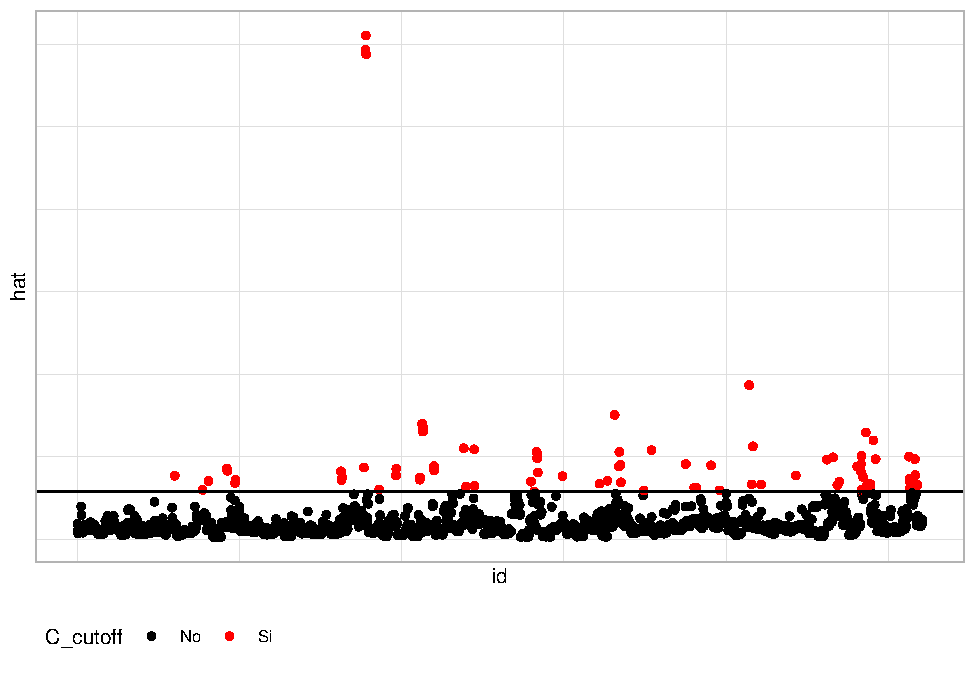
\includegraphics{06-Regresión_files/figure-latex/hat-1.pdf}

Dado que esta última técnica es empírica, se puede observar en el gráfico anterior que hay varias observaciones posiblemente influyentes en el conjunto de datos de la muestra de hogares.

\hypertarget{inferencia-sobre-los-paruxe1metros-del-modelo}{%
\section{Inferencia sobre los parámetros del Modelo}\label{inferencia-sobre-los-paruxe1metros-del-modelo}}

Una vez evaluado el correcto ajuste del modelo utilizando las metodologías vistas anteriormente y corroborando las propiedades distribucionales de los errores y por ende, de la variable respuesta \(y\), el paso siguiente es verificar si los parámetros estimados son significativos y por ende, las covariables utilizadas para ajustar el modelo aportan significativamente para explicar o predecir a la variable de estudio \(y\).

Dada las propiedades distribucionales de los \(\beta's\), un estadístico de prueba natural para evaluar la significancia de dicho parámetro se basa en la distribución ``t-student'' y se describe a continuación:

\[
t=\frac{\hat{\beta}_{k}-\beta_{k}}{se\left(\hat{\beta}_{k}\right)}\sim t_{n-p}
\]

Donde \(p\) es el número de parámetros del modelo y \(n\) el tamaño de la muestra de la encuesta. En este sentido, el estadístico de prueba anterior evalúa las hipótesis \(H_{0}:\beta_{k}=0\) versus la alternativa \(H_{1}:\beta_{k}\neq0\).

De las propiedades distribucionales de los \(\beta\), se puede construir un intervalo de confianza al \((1-\alpha)\times100\%\) para \(\beta_{k}\) está dado por:

\[
\hat{\beta}_{k}\pm t_{1-\frac{\alpha}{2},\,df}\,se\left(\hat{\beta}_{k}\right)
\]

Donde, los grados de libertad para el intervalo (\(df\)) en una encuesta de hogares (muestras complejas) está dado por el número de conglomerados finales de la primera etapa menos el número de estratos de la etapa primaria \(\left(df=\sum_{h}a_{h}-H\right)\).

Para la aplicación de las temáticas vistas, es decir, realizar la prueba de hipótesis y los intervalos de confianza para los parámetros utilizaremos el modelo que se ha venido trabajando y aplicaremos las funciones \texttt{summary.svyglm} para las pruebas t y \texttt{confint.svyglm} para los intervalos de confianza como sigue:

\begin{Shaded}
\begin{Highlighting}[]
\NormalTok{survey}\SpecialCharTok{:::}\FunctionTok{summary.svyglm}\NormalTok{(mod\_svy)}
\end{Highlighting}
\end{Shaded}

\begin{verbatim}
## 
## Call:
## svyglm(formula = Income ~ Expenditure + Zone + Sex + Age2, design = diseno_qwgt)
## 
## Survey design:
## Called via srvyr
## 
## Coefficients:
##             Estimate Std. Error t value Pr(>|t|)    
## (Intercept) 62.18419   62.98928    0.99     0.33    
## Expenditure  1.22548    0.19798    6.19  9.5e-09 ***
## ZoneUrban   63.46000   40.09025    1.58     0.12    
## SexMale     21.73256   15.78081    1.38     0.17    
## Age2         0.00852    0.00557    1.53     0.13    
## ---
## Signif. codes:  0 '***' 0.001 '**' 0.01 '*' 0.05 '.' 0.1 ' ' 1
## 
## (Dispersion parameter for gaussian family taken to be 118297)
## 
## Number of Fisher Scoring iterations: 2
\end{verbatim}

\begin{Shaded}
\begin{Highlighting}[]
\NormalTok{survey}\SpecialCharTok{:::}\FunctionTok{confint.svyglm}\NormalTok{(mod\_svy)}
\end{Highlighting}
\end{Shaded}

\begin{tabular}{l|r|r}
\hline
  & 2.5 \% & 97.5 \%\\
\hline
(Intercept) & -62.5855 & 186.9538\\
\hline
Expenditure & 0.8333 & 1.6176\\
\hline
ZoneUrban & -15.9511 & 142.8711\\
\hline
SexMale & -9.5262 & 52.9913\\
\hline
Age2 & -0.0025 & 0.0196\\
\hline
\end{tabular}

De lo anterior se puede observar que, con una confianza del 95\% el único parámetro significativo del modelo es Expenditure y ese mismo resultado lo reflejan los intervalos de confianza.

\emph{Estimación de una observación}

Los modelos de regresión lineales, según \emph{(Neter et al., 1996).}, son utilizado esencialmente con 2 fines, el primero es tratar de explicar la variable respuesta en términos de covariables que pueden encontrarse en la encuesta o en registros administrativos, censos, etc. Adicionalmente, también son usados para predecir valores de la variable en estudio ya sea dentro del intervalo de valores recogidos en la muestra o por fuera de dicho intervalo. Lo primero se ha abordado a lo largo de todo el capítulo y lo segundo se obtiene de la siguiente manera:

\[
\hat{E}(y_{i}\mid\boldsymbol{x}_{obs,i})=\boldsymbol{x}_{obs,i}\hat{\boldsymbol{\beta}}
\]

De manera explícita, si se ajusta un modelo con 4 covariables la expresión sería:

\[
\hat{E}(y_{i}\mid\boldsymbol{x}_{obs,i})=\hat{\beta}_{0}+\hat{\beta}_{1}x_{1i}+\hat{\beta}_{2}x_{2i}+\hat{\beta}_{3}x_{3i}+\hat{\beta}_{4}x_{4i}
\]

La varianza de la estimación se calcula de la siguiente manera:

\[
var\left(\hat{E}\left(y_{i}\mid x_{obs,i}\right)\right) 
=  x'_{obs,i}cov\left(\hat{\beta}\right)x{}_{obs,i}
\]

A continuación, se presenta cómo se realiza la estimación del valor esperado, primero se estiman los parámetros del modelo:

\begin{tabular}{l|r|r|r|r}
\hline
term & estimate & std.error & statistic & p.value\\
\hline
(Intercept) & 62.1842 & 62.9893 & 0.9872 & 0.3256\\
\hline
Expenditure & 1.2255 & 0.1980 & 6.1901 & 0.0000\\
\hline
ZoneUrban & 63.4600 & 40.0902 & 1.5829 & 0.1162\\
\hline
SexMale & 21.7326 & 15.7808 & 1.3772 & 0.1711\\
\hline
Age2 & 0.0085 & 0.0056 & 1.5297 & 0.1288\\
\hline
\end{tabular}

Por lo anterior, la estimación del valor esperado o predicción queda:

\[
\hat{E}(y_{i}\mid\boldsymbol{x}_{obs,i})=62.2+1.2x_{1i}+63.5x_{2i}+21.7x_{3i}+0.01x_{4i}
\]
Para calcular la varianza de la estimación, primero se deben obtener las varianzas de la estimación de los parámetros:

\begin{Shaded}
\begin{Highlighting}[]
\FunctionTok{vcov}\NormalTok{(mod\_svy)}
\end{Highlighting}
\end{Shaded}

\begin{tabular}{l|r|r|r|r|r}
\hline
  & (Intercept) & Expenditure & ZoneUrban & SexMale & Age2\\
\hline
(Intercept) & 3967.6496 & -11.3101 & 275.9858 & 312.4533 & -0.1852\\
\hline
Expenditure & -11.3101 & 0.0392 & -3.5526 & -0.5004 & 0.0005\\
\hline
ZoneUrban & 275.9858 & -3.5526 & 1607.2280 & -130.7108 & -0.0559\\
\hline
SexMale & 312.4533 & -0.5004 & -130.7108 & 249.0339 & -0.0043\\
\hline
Age2 & -0.1852 & 0.0005 & -0.0559 & -0.0043 & 0.0000\\
\hline
\end{tabular}

Ahora bien, se procede a realizar los cálculos como lo indica la expresión mostrada anteriormente:

\begin{Shaded}
\begin{Highlighting}[]
\NormalTok{xobs }\OtherTok{\textless{}{-}} \FunctionTok{model.matrix}\NormalTok{(mod\_svy) }\SpecialCharTok{\%\textgreater{}\%}
        \FunctionTok{data.frame}\NormalTok{() }\SpecialCharTok{\%\textgreater{}\%} \FunctionTok{slice}\NormalTok{(}\DecValTok{1}\NormalTok{) }\SpecialCharTok{\%\textgreater{}\%} \FunctionTok{as.matrix}\NormalTok{()}

\NormalTok{cov\_beta }\OtherTok{\textless{}{-}} \FunctionTok{vcov}\NormalTok{(mod\_svy) }\SpecialCharTok{\%\textgreater{}\%} \FunctionTok{as.matrix}\NormalTok{()}

\FunctionTok{as.numeric}\NormalTok{(xobs }\SpecialCharTok{\%*\%}\NormalTok{ cov\_beta }\SpecialCharTok{\%*\%} \FunctionTok{t}\NormalTok{(xobs))}
\end{Highlighting}
\end{Shaded}

\begin{verbatim}
## [1] 1921
\end{verbatim}

Si el objetivo ahora es calcular el intervalo de confianza para la predicción se utiliza la siguiente ecuación:

\[
\boldsymbol{x}_{obs,i}\hat{\beta}\pm t_{\left(1-\frac{\alpha}{2},n-p\right)}\sqrt{var\left(\hat{E}\left(y_{i}\mid\boldsymbol{x}_{obs,i}\right)\right)}
\]

Para realizar los cálculos en R, se utiliza la función \texttt{confint} y \texttt{predict} como sigue:

\begin{Shaded}
\begin{Highlighting}[]
\NormalTok{pred }\OtherTok{\textless{}{-}} \FunctionTok{data.frame}\NormalTok{(}\FunctionTok{predict}\NormalTok{(mod\_svy, }\AttributeTok{type =} \StringTok{"link"}\NormalTok{))}
\NormalTok{pred\_IC }\OtherTok{\textless{}{-}} \FunctionTok{data.frame}\NormalTok{(}\FunctionTok{confint}\NormalTok{(}\FunctionTok{predict}\NormalTok{(mod\_svy, }\AttributeTok{type =} \StringTok{"link"}\NormalTok{)))}
\FunctionTok{colnames}\NormalTok{(pred\_IC) }\OtherTok{\textless{}{-}} \FunctionTok{c}\NormalTok{(}\StringTok{"Lim\_Inf"}\NormalTok{, }\StringTok{"Lim\_Sup"}\NormalTok{)}
\NormalTok{pred\_IC}
\end{Highlighting}
\end{Shaded}

Ahora, de manera gráfica las predicciones e intervalos se vería de la siguiente manera:

\begin{Shaded}
\begin{Highlighting}[]
\NormalTok{pred }\OtherTok{\textless{}{-}} \FunctionTok{bind\_cols}\NormalTok{(pred, pred\_IC)}
\NormalTok{pred}\SpecialCharTok{$}\NormalTok{Expenditure }\OtherTok{\textless{}{-}}\NormalTok{ encuesta}\SpecialCharTok{$}\NormalTok{Expenditure}
\NormalTok{pred }\SpecialCharTok{\%\textgreater{}\%} \FunctionTok{slice}\NormalTok{(}\DecValTok{1}\SpecialCharTok{:}\NormalTok{6L)}
\NormalTok{pd }\OtherTok{\textless{}{-}} \FunctionTok{position\_dodge}\NormalTok{(}\AttributeTok{width =} \FloatTok{0.2}\NormalTok{)}
\FunctionTok{ggplot}\NormalTok{(pred }\SpecialCharTok{\%\textgreater{}\%} \FunctionTok{slice}\NormalTok{(}\DecValTok{1}\SpecialCharTok{:}\NormalTok{100L),}
       \FunctionTok{aes}\NormalTok{(}\AttributeTok{x =}\NormalTok{ Expenditure , }\AttributeTok{y =}\NormalTok{ link)) }\SpecialCharTok{+}
  \FunctionTok{geom\_errorbar}\NormalTok{(}\FunctionTok{aes}\NormalTok{(}\AttributeTok{ymin =}\NormalTok{ Lim\_Inf,}
                    \AttributeTok{ymax =}\NormalTok{ Lim\_Sup),}
                \AttributeTok{width =}\NormalTok{ .}\DecValTok{1}\NormalTok{,}
                \AttributeTok{linetype =} \DecValTok{1}\NormalTok{) }\SpecialCharTok{+}
  \FunctionTok{geom\_point}\NormalTok{(}\AttributeTok{size =} \DecValTok{2}\NormalTok{, }\AttributeTok{position =}\NormalTok{ pd) }\SpecialCharTok{+}
  \FunctionTok{theme\_bw}\NormalTok{()}
\end{Highlighting}
\end{Shaded}

Por último, si el interés es hacer una predicción fuera del rango de valores que fue capturado en la muestra. Para esto, supongamos que se desea predecir:

\begin{Shaded}
\begin{Highlighting}[]
\NormalTok{datos\_nuevos }\OtherTok{\textless{}{-}} \FunctionTok{data.frame}\NormalTok{(}\AttributeTok{Expenditure =} \DecValTok{1600}\NormalTok{, }
                           \AttributeTok{Age2 =} \DecValTok{40}\SpecialCharTok{\^{}}\DecValTok{2}\NormalTok{, }\AttributeTok{Sex =} \StringTok{"Male"}\NormalTok{, }
                           \AttributeTok{Zone =} \StringTok{"Urban"}\NormalTok{)}
\end{Highlighting}
\end{Shaded}

La varianza para la predicción se hace siguiendo la siguiente ecuación:

\[
var\left(\hat{E}\left(y_{i}\mid\boldsymbol{x}_{obs,i}\right)\right)=\boldsymbol{x}_{obs,i}^{t}cov\left(\boldsymbol{\beta}\right)\boldsymbol{x}_{obs,i} + \hat{\sigma}^2_{yx}
\]

Por tanto, se construye la matriz de observaciones y se calcula la varianza como sigue:

\begin{Shaded}
\begin{Highlighting}[]
\NormalTok{x\_noObs }\OtherTok{=} \FunctionTok{matrix}\NormalTok{(}\FunctionTok{c}\NormalTok{(}\DecValTok{1}\NormalTok{,}\DecValTok{1600}\NormalTok{,}\DecValTok{1}\NormalTok{,}\DecValTok{1}\NormalTok{,}\DecValTok{40}\SpecialCharTok{\^{}}\DecValTok{2}\NormalTok{),}\AttributeTok{nrow =} \DecValTok{1}\NormalTok{)}
\FunctionTok{as.numeric}\NormalTok{(}\FunctionTok{sqrt}\NormalTok{(x\_noObs}\SpecialCharTok{\%*\%}\NormalTok{cov\_beta}\SpecialCharTok{\%*\%}\FunctionTok{t}\NormalTok{(x\_noObs)))}
\end{Highlighting}
\end{Shaded}

\begin{verbatim}
## [1] 244.6
\end{verbatim}

Por último, el intervalo de confianza sigue la siguiente ecuación:

\[
\boldsymbol{x}_{obs,i}\hat{\beta}\pm t_{\left(1-\frac{\alpha}{2},n-p\right)}\sqrt{var\left(\hat{E}\left(y_{i}\mid\boldsymbol{x}_{obs,i}\right)\right)+\hat{\sigma}_{yx}^{2}}
\]
En \texttt{R} se hace la predicción de la siguiente manera:

\begin{Shaded}
\begin{Highlighting}[]
\FunctionTok{predict}\NormalTok{(mod\_svy, }\AttributeTok{newdata =}\NormalTok{ datos\_nuevos, }\AttributeTok{type =}  \StringTok{"link"}\NormalTok{)}
\end{Highlighting}
\end{Shaded}

\begin{verbatim}
##   link  SE
## 1 2122 245
\end{verbatim}

y el intervalo:

\begin{Shaded}
\begin{Highlighting}[]
\FunctionTok{confint}\NormalTok{(}\FunctionTok{predict}\NormalTok{(mod\_svy,}\AttributeTok{newdata =}\NormalTok{ datos\_nuevos))}
\end{Highlighting}
\end{Shaded}

\begin{tabular}{r|r}
\hline
2.5 \% & 97.5 \%\\
\hline
1642 & 2601\\
\hline
\end{tabular}

\hypertarget{gruxe1ficas-en-r}{%
\chapter{Gráficas en R}\label{gruxe1ficas-en-r}}

El objetivo de esta capítulo es mostrarle al lector cómo hacer gráficos generales en \texttt{R}. En todo análisis de encuestas, el componente gráfico es fundamental para revisar tendencias en algunas variables de interés. También son muy necesarias las gráficas cuando se el objetivo es chequear algunos supuestos en el ajustes de modelo, por ejemplo, varianza constante en los errores, normalidad, etc.

Uno de los paquetes más usados para graficar en \texttt{R} es ggplot2 el cual es un paquete potente y flexible, implementado por Hadley Wickham, para producir gráficos elegantes. El gg en ggplot2 significa Grammar of Graphics, el cual es un concepto gráfico que describe gráficos usando gramática.

Como es de costumbre, se inicia este capítulo cargando las librerías y bases de datos:

\begin{Shaded}
\begin{Highlighting}[]
\CommentTok{\# knitr::opts\_chunk$set(cache = TRUE, warning = FALSE, message = FALSE, error = FALSE)}
\FunctionTok{options}\NormalTok{(}\AttributeTok{digits =} \DecValTok{4}\NormalTok{)}
\FunctionTok{library}\NormalTok{(survey)}
\FunctionTok{library}\NormalTok{(srvyr)}
\FunctionTok{library}\NormalTok{(convey)}
\FunctionTok{library}\NormalTok{(TeachingSampling)}
\FunctionTok{library}\NormalTok{(printr)}
\FunctionTok{library}\NormalTok{(ggplot2)}
\FunctionTok{library}\NormalTok{(patchwork)}
\end{Highlighting}
\end{Shaded}

El cargue de la base de datos se hace a continuación,

\begin{Shaded}
\begin{Highlighting}[]
\FunctionTok{data}\NormalTok{(BigCity, }\AttributeTok{package =} \StringTok{"TeachingSampling"}\NormalTok{)}
\NormalTok{encuesta }\OtherTok{\textless{}{-}} \FunctionTok{readRDS}\NormalTok{(}\StringTok{"Data/encuesta.rds"}\NormalTok{)}
\end{Highlighting}
\end{Shaded}

A continuación, se define el diseño de muestreo:

\begin{Shaded}
\begin{Highlighting}[]
\FunctionTok{library}\NormalTok{(srvyr)}
\NormalTok{diseno }\OtherTok{\textless{}{-}}\NormalTok{ encuesta }\SpecialCharTok{\%\textgreater{}\%}
  \FunctionTok{as\_survey\_design}\NormalTok{(}
    \AttributeTok{strata =}\NormalTok{ Stratum,}
    \AttributeTok{ids =}\NormalTok{ PSU,}
    \AttributeTok{weights =}\NormalTok{ wk,}
    \AttributeTok{nest =}\NormalTok{ T}
\NormalTok{  )}
\end{Highlighting}
\end{Shaded}

A partir de las variables de la encuesta, para efectos de los ejemplos, se definen las siguientes variables:

\begin{Shaded}
\begin{Highlighting}[]
\NormalTok{diseno }\OtherTok{\textless{}{-}}\NormalTok{ diseno }\SpecialCharTok{\%\textgreater{}\%} \FunctionTok{mutate}\NormalTok{(}
  \AttributeTok{pobreza =} \FunctionTok{ifelse}\NormalTok{(Poverty }\SpecialCharTok{!=} \StringTok{"NotPoor"}\NormalTok{, }\DecValTok{1}\NormalTok{, }\DecValTok{0}\NormalTok{),}
  \AttributeTok{desempleo =} \FunctionTok{ifelse}\NormalTok{(Employment }\SpecialCharTok{==} \StringTok{"Unemployed"}\NormalTok{, }\DecValTok{1}\NormalTok{, }\DecValTok{0}\NormalTok{),}
  \AttributeTok{edad\_18 =} \FunctionTok{case\_when}\NormalTok{(}
\NormalTok{    Age }\SpecialCharTok{\textless{}} \DecValTok{18} \SpecialCharTok{\textasciitilde{}} \StringTok{"\textless{} 18 años"}\NormalTok{,}
    \ConstantTok{TRUE} \SpecialCharTok{\textasciitilde{}} \StringTok{"\textgreater{}= 18 años"}
\NormalTok{  )}
\NormalTok{)}
\end{Highlighting}
\end{Shaded}

Como se mostró en capítulos anteriores, se divide la muestra en sub grupos para ejemplificar los conceptos que se mostrarán en este capítulo:

\begin{Shaded}
\begin{Highlighting}[]
\NormalTok{sub\_Urbano }\OtherTok{\textless{}{-}}\NormalTok{ diseno }\SpecialCharTok{\%\textgreater{}\%} \FunctionTok{filter}\NormalTok{(Zone }\SpecialCharTok{==} \StringTok{"Urban"}\NormalTok{)}
\NormalTok{sub\_Rural }\OtherTok{\textless{}{-}}\NormalTok{ diseno }\SpecialCharTok{\%\textgreater{}\%} \FunctionTok{filter}\NormalTok{(Zone }\SpecialCharTok{==} \StringTok{"Rural"}\NormalTok{)}
\NormalTok{sub\_Mujer }\OtherTok{\textless{}{-}}\NormalTok{ diseno }\SpecialCharTok{\%\textgreater{}\%} \FunctionTok{filter}\NormalTok{(Sex }\SpecialCharTok{==} \StringTok{"Female"}\NormalTok{)}
\NormalTok{sub\_Hombre }\OtherTok{\textless{}{-}}\NormalTok{ diseno }\SpecialCharTok{\%\textgreater{}\%} \FunctionTok{filter}\NormalTok{(Sex }\SpecialCharTok{==} \StringTok{"Male"}\NormalTok{)}
\end{Highlighting}
\end{Shaded}

Para crear las gráficas en este texto se utilizará por defecto el tema que la CEPAL tiene asignado por defecto. El tema se define a continuación:

\begin{Shaded}
\begin{Highlighting}[]
\NormalTok{theme\_cepal }\OtherTok{\textless{}{-}} \ControlFlowTok{function}\NormalTok{(...) \{}
  \FunctionTok{theme\_light}\NormalTok{(}\DecValTok{10}\NormalTok{) }\SpecialCharTok{+}
    \FunctionTok{theme}\NormalTok{(}
      \AttributeTok{axis.text.x =} \FunctionTok{element\_blank}\NormalTok{(),}
      \AttributeTok{axis.ticks.x =} \FunctionTok{element\_blank}\NormalTok{(),}
      \AttributeTok{axis.text.y =} \FunctionTok{element\_blank}\NormalTok{(),}
      \AttributeTok{axis.ticks.y =} \FunctionTok{element\_blank}\NormalTok{(),}
      \AttributeTok{legend.position =} \StringTok{"bottom"}\NormalTok{,}
      \AttributeTok{legend.justification =} \StringTok{"left"}\NormalTok{,}
      \AttributeTok{legend.direction =} \StringTok{"horizontal"}\NormalTok{,}
      \AttributeTok{plot.title =} \FunctionTok{element\_text}\NormalTok{(}\AttributeTok{size =} \DecValTok{20}\NormalTok{, }\AttributeTok{hjust =} \FloatTok{0.5}\NormalTok{),}
\NormalTok{      ...}
\NormalTok{    )}
\NormalTok{\}}
\end{Highlighting}
\end{Shaded}

\hypertarget{histogramas-para-graficar-variables-continuas.}{%
\section{Histogramas para graficar variables continuas.}\label{histogramas-para-graficar-variables-continuas.}}

Un histograma es una representación gráfica de los datos de una variable empleando
rectángulos (barras) cuya altura es proporcional a la frecuencia de los valores representados y su ancho proporcional a la amplitud de los intervalos de la clase.

Como se mencionó anteriormente, las gráficas se realizarán principalmente con la librería \texttt{ggplot2}y nos apoyamos en la librería \texttt{patchwork} para organizar la visual de las gráficas. A continuacuón, se presenta cómo realizar un histograma para la variable ingresos utilizando los factores de expansión de la encuesta. EN primera instancia se define la fuente de información (data), luego se definen la variable a graficar (x) y los pesos de muestreo (weight). Una vez definido los parámetros generales del gráfico se define el tipo de gráfico, que para nuestro caso como es un histograma es geom\_histogram. Se definen los títulos que se quiere que tenga el histograma y por último, se aplica el tema de la CEPAL.

\begin{Shaded}
\begin{Highlighting}[]
\NormalTok{plot1\_Ponde }\OtherTok{\textless{}{-}} \FunctionTok{ggplot}\NormalTok{(}
  \AttributeTok{data =}\NormalTok{ encuesta,              }
  \FunctionTok{aes}\NormalTok{(}\AttributeTok{x =}\NormalTok{ Income, }\AttributeTok{weight =}\NormalTok{ wk)) }\SpecialCharTok{+}
  \FunctionTok{geom\_histogram}\NormalTok{(               }
    \FunctionTok{aes}\NormalTok{(}\AttributeTok{y =}\NormalTok{ ..density..)) }\SpecialCharTok{+}        
  \FunctionTok{ylab}\NormalTok{(}\StringTok{""}\NormalTok{) }\SpecialCharTok{+}                   
  \FunctionTok{ggtitle}\NormalTok{(}\StringTok{"Ponderado"}\NormalTok{) }\SpecialCharTok{+}        
  \FunctionTok{theme\_cepal}\NormalTok{()  }
\NormalTok{plot1\_Ponde}
\end{Highlighting}
\end{Shaded}

\includegraphics{07-Gráficas_files/figure-latex/hist1-1.pdf}

De forma análoga se define el siguiente histograma, note que en este caso se omitió el parámetro \texttt{weight}. Es decir, se genera un histograma sin pesos de muestreo:

\begin{Shaded}
\begin{Highlighting}[]
\NormalTok{plot1\_SinPonde }\OtherTok{\textless{}{-}}
  \FunctionTok{ggplot}\NormalTok{(encuesta, }\FunctionTok{aes}\NormalTok{(}\AttributeTok{x =}\NormalTok{ Income)) }\SpecialCharTok{+}
  \FunctionTok{geom\_histogram}\NormalTok{(}\FunctionTok{aes}\NormalTok{(}\AttributeTok{y =}\NormalTok{ ..density..)) }\SpecialCharTok{+}
  \FunctionTok{ylab}\NormalTok{(}\StringTok{""}\NormalTok{) }\SpecialCharTok{+}
  \FunctionTok{ggtitle}\NormalTok{(}\StringTok{"Sin ponderar"}\NormalTok{) }\SpecialCharTok{+}
  \FunctionTok{theme\_cepal}\NormalTok{()}
\NormalTok{plot1\_SinPonde}
\end{Highlighting}
\end{Shaded}

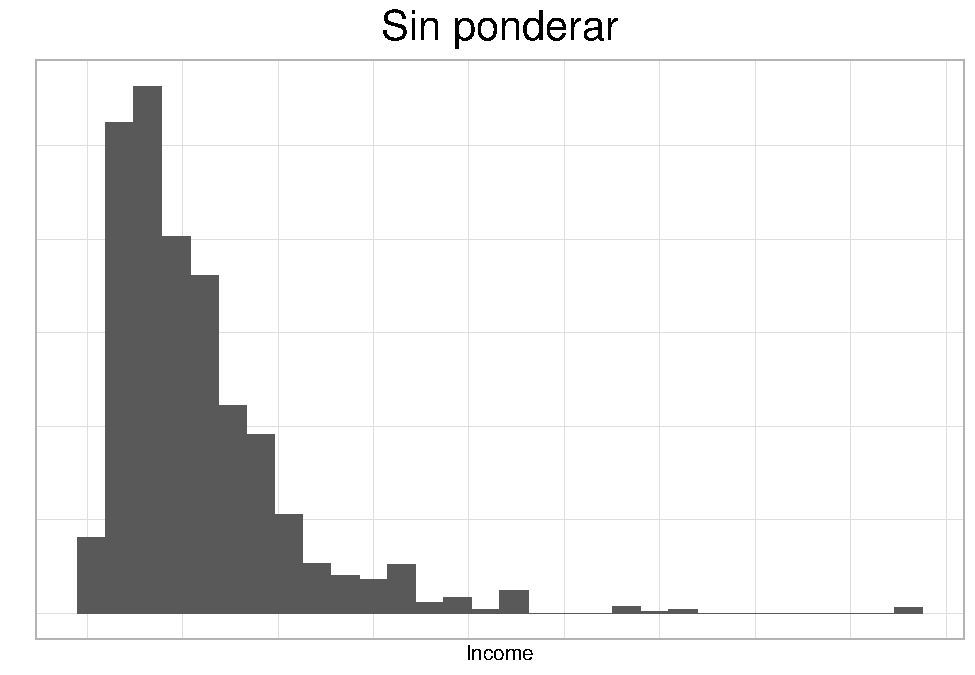
\includegraphics{07-Gráficas_files/figure-latex/hist1a-1.pdf}

Ahora bien, para efectos de comparación, se grafica la variable ingreso tomada de la población (BigCity) y se muestran los tres histogramas para notar las diferencias que tienen en comparación con el poblacional.

\begin{Shaded}
\begin{Highlighting}[]
\NormalTok{plot1\_censo }\OtherTok{\textless{}{-}} \FunctionTok{ggplot}\NormalTok{(BigCity, }\FunctionTok{aes}\NormalTok{(}\AttributeTok{x =}\NormalTok{ Income)) }\SpecialCharTok{+}
  \FunctionTok{geom\_histogram}\NormalTok{(}\FunctionTok{aes}\NormalTok{(}\AttributeTok{y =}\NormalTok{ ..density..)) }\SpecialCharTok{+}
  \FunctionTok{ylab}\NormalTok{(}\StringTok{""}\NormalTok{) }\SpecialCharTok{+}
  \FunctionTok{ggtitle}\NormalTok{(}\StringTok{"Poblacional"}\NormalTok{) }\SpecialCharTok{+}
  \FunctionTok{theme\_cepal}\NormalTok{() }\SpecialCharTok{+}
  \FunctionTok{xlim}\NormalTok{(}\DecValTok{0}\NormalTok{, }\DecValTok{2500}\NormalTok{)}

\NormalTok{plot1\_censo }\SpecialCharTok{|}\NormalTok{ plot1\_Ponde }\SpecialCharTok{|}\NormalTok{ plot1\_SinPonde}
\end{Highlighting}
\end{Shaded}

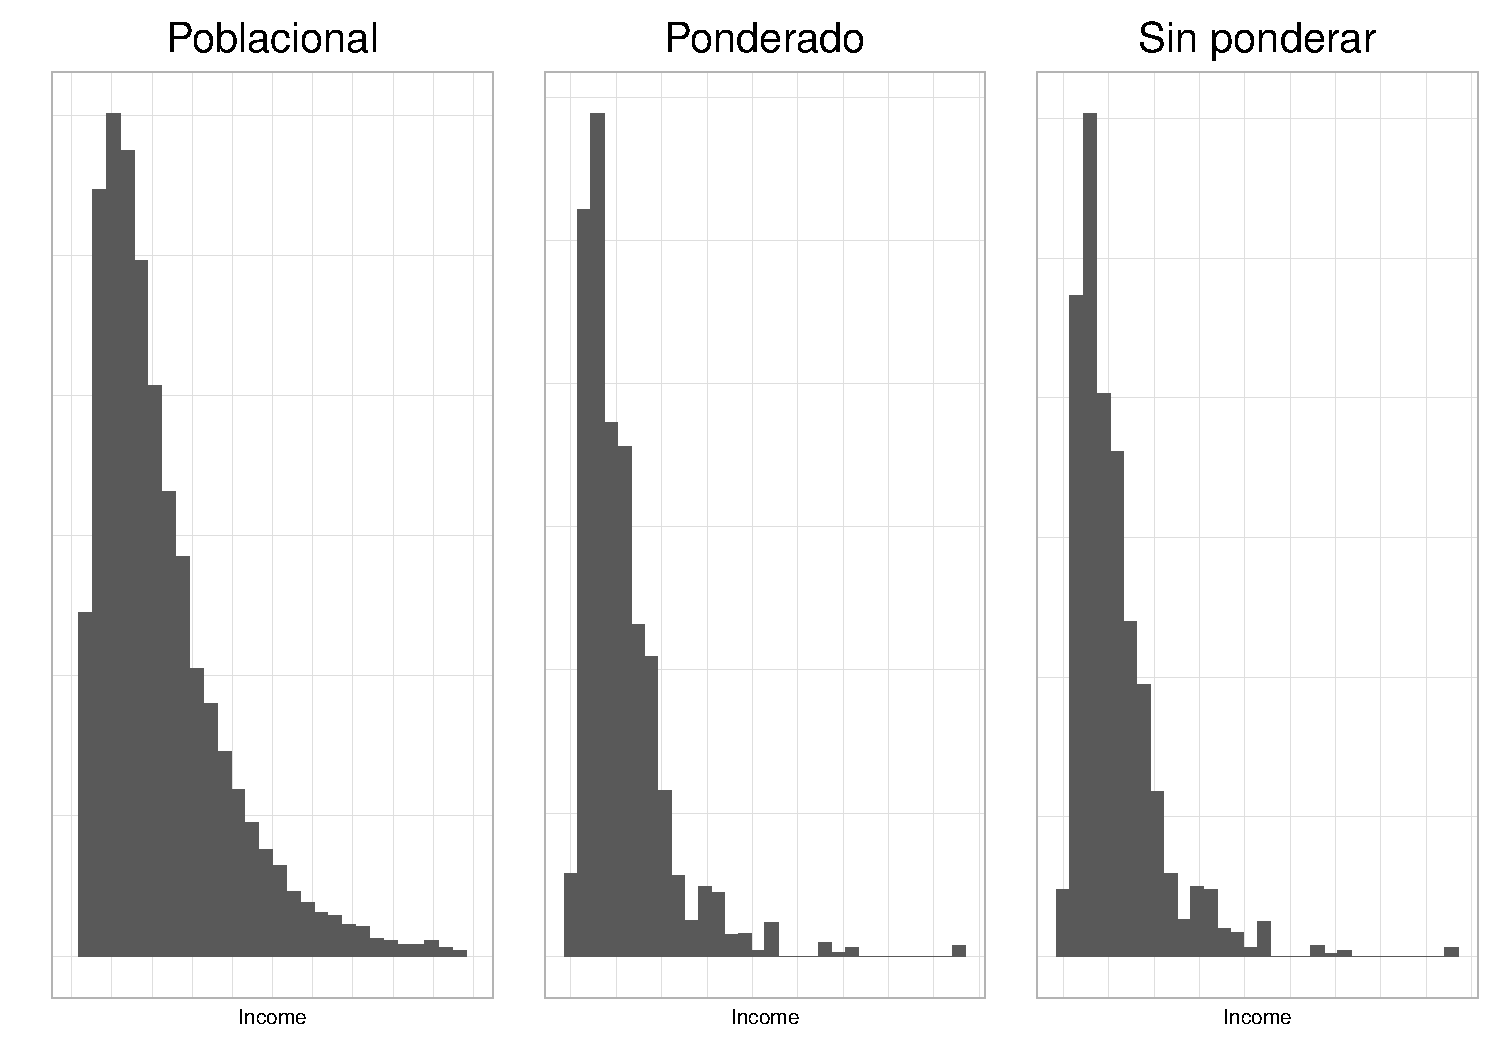
\includegraphics{07-Gráficas_files/figure-latex/hist1b-1.pdf}

Por otro lado, repetimos ahora la secuencia de gráficos pero en este caso para la variable \emph{Expenditure}:

\begin{Shaded}
\begin{Highlighting}[]
\NormalTok{plot2\_Ponde }\OtherTok{\textless{}{-}} \FunctionTok{ggplot}\NormalTok{(}
  \AttributeTok{data =}\NormalTok{  encuesta,}
  \FunctionTok{aes}\NormalTok{(}\AttributeTok{x =}\NormalTok{ Expenditure, }\AttributeTok{weight =}\NormalTok{ wk)}
\NormalTok{) }\SpecialCharTok{+}
  \FunctionTok{geom\_histogram}\NormalTok{(}\FunctionTok{aes}\NormalTok{(}\AttributeTok{y =}\NormalTok{ ..density..)) }\SpecialCharTok{+}
  \FunctionTok{ylab}\NormalTok{(}\StringTok{""}\NormalTok{) }\SpecialCharTok{+}
  \FunctionTok{ggtitle}\NormalTok{(}\StringTok{"Ponderado"}\NormalTok{) }\SpecialCharTok{+}
  \FunctionTok{theme\_cepal}\NormalTok{()}
\NormalTok{plot2\_Ponde}
\end{Highlighting}
\end{Shaded}

\includegraphics{07-Gráficas_files/figure-latex/hist2-1.pdf}

\begin{Shaded}
\begin{Highlighting}[]
\NormalTok{plot2\_SinPonde }\OtherTok{\textless{}{-}} \FunctionTok{ggplot}\NormalTok{(}\AttributeTok{data =}\NormalTok{ encuesta,}
      \FunctionTok{aes}\NormalTok{(}\AttributeTok{x =}\NormalTok{ Expenditure)) }\SpecialCharTok{+}
      \FunctionTok{geom\_histogram}\NormalTok{(}\FunctionTok{aes}\NormalTok{(}\AttributeTok{y =}\NormalTok{ ..density..)) }\SpecialCharTok{+}
      \FunctionTok{ylab}\NormalTok{(}\StringTok{""}\NormalTok{) }\SpecialCharTok{+}
      \FunctionTok{ggtitle}\NormalTok{(}\StringTok{"Sin ponderar"}\NormalTok{) }\SpecialCharTok{+}
      \FunctionTok{theme\_cepal}\NormalTok{()}
\NormalTok{plot2\_SinPonde}
\end{Highlighting}
\end{Shaded}

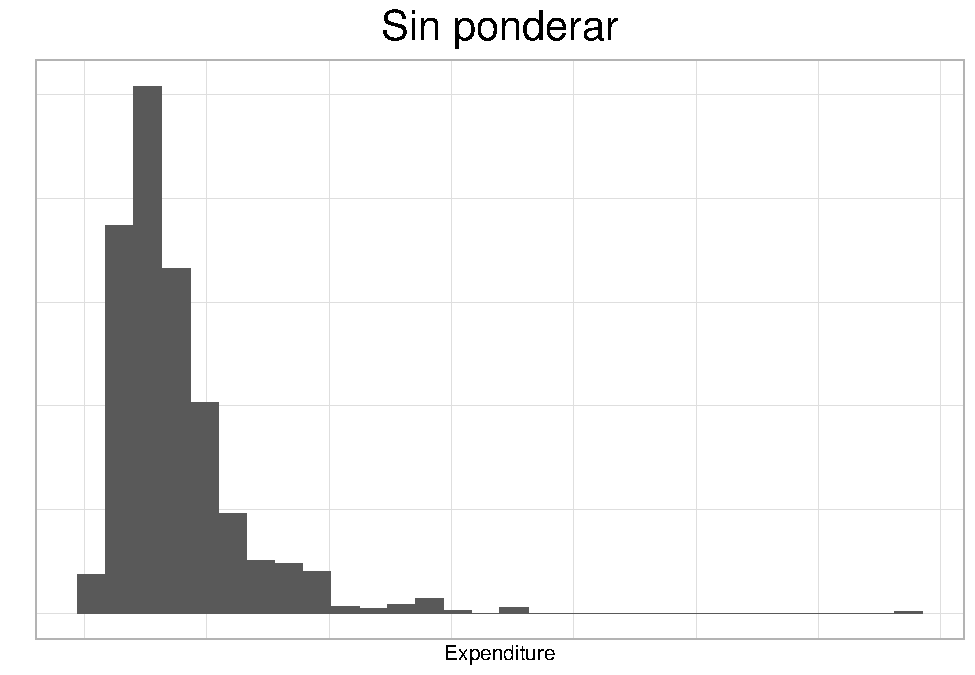
\includegraphics{07-Gráficas_files/figure-latex/hist2a-1.pdf}

\begin{Shaded}
\begin{Highlighting}[]
\NormalTok{plot2\_censo }\OtherTok{\textless{}{-}} \FunctionTok{ggplot}\NormalTok{(BigCity, }\FunctionTok{aes}\NormalTok{(}\AttributeTok{x =}\NormalTok{ Expenditure)) }\SpecialCharTok{+}
  \FunctionTok{geom\_histogram}\NormalTok{(}\FunctionTok{aes}\NormalTok{(}\AttributeTok{y =}\NormalTok{ ..density..)) }\SpecialCharTok{+}
  \FunctionTok{ylab}\NormalTok{(}\StringTok{""}\NormalTok{) }\SpecialCharTok{+}
  \FunctionTok{ggtitle}\NormalTok{(}\StringTok{"Poblacional"}\NormalTok{) }\SpecialCharTok{+}
  \FunctionTok{theme\_cepal}\NormalTok{() }\SpecialCharTok{+}
  \FunctionTok{xlim}\NormalTok{(}\DecValTok{0}\NormalTok{, }\DecValTok{1500}\NormalTok{)}

\NormalTok{plot2\_censo }\SpecialCharTok{|}\NormalTok{ plot2\_Ponde }\SpecialCharTok{|}\NormalTok{ plot2\_SinPonde}
\end{Highlighting}
\end{Shaded}

Como conclusión, de ambos ejercicios, se puede observar que el histograma que mejor se aproxima al poblacional es aquel que utiliza los pesos de muestreo, aunque el gráfico que no los utiliza se aproxima bien y esto debido a la correcta selección de la muestra.

Por otro lado, cuando el interés ahora es realizar comparaciones entre dos o más agrupaciones, es posible hacer uso del parámetro \texttt{fill}, el cual ``rellena'' las barras del histograma con diferentes colores según sea el grupo. Para este ejemplo, se van a graficar subgrupos por zonas:

\begin{Shaded}
\begin{Highlighting}[]
\NormalTok{plot3\_Ponde }\OtherTok{\textless{}{-}} \FunctionTok{ggplot}\NormalTok{(}
\NormalTok{  encuesta,}
  \FunctionTok{aes}\NormalTok{(}\AttributeTok{x =}\NormalTok{ Income, }\AttributeTok{weight =}\NormalTok{ wk)) }\SpecialCharTok{+}
  \FunctionTok{geom\_histogram}\NormalTok{(}
    \FunctionTok{aes}\NormalTok{(}\AttributeTok{y =}\NormalTok{ ..density.., }\AttributeTok{fill =}\NormalTok{ Zone),}
    \AttributeTok{alpha =} \FloatTok{0.5}\NormalTok{,}
     \AttributeTok{position =} \StringTok{"identity"} 
\NormalTok{  ) }\SpecialCharTok{+}
  \FunctionTok{ylab}\NormalTok{(}\StringTok{""}\NormalTok{) }\SpecialCharTok{+}
  \FunctionTok{ggtitle}\NormalTok{(}\StringTok{"Ponderado"}\NormalTok{) }\SpecialCharTok{+}
  \FunctionTok{theme\_cepal}\NormalTok{()}
\NormalTok{plot3\_Ponde}
\end{Highlighting}
\end{Shaded}

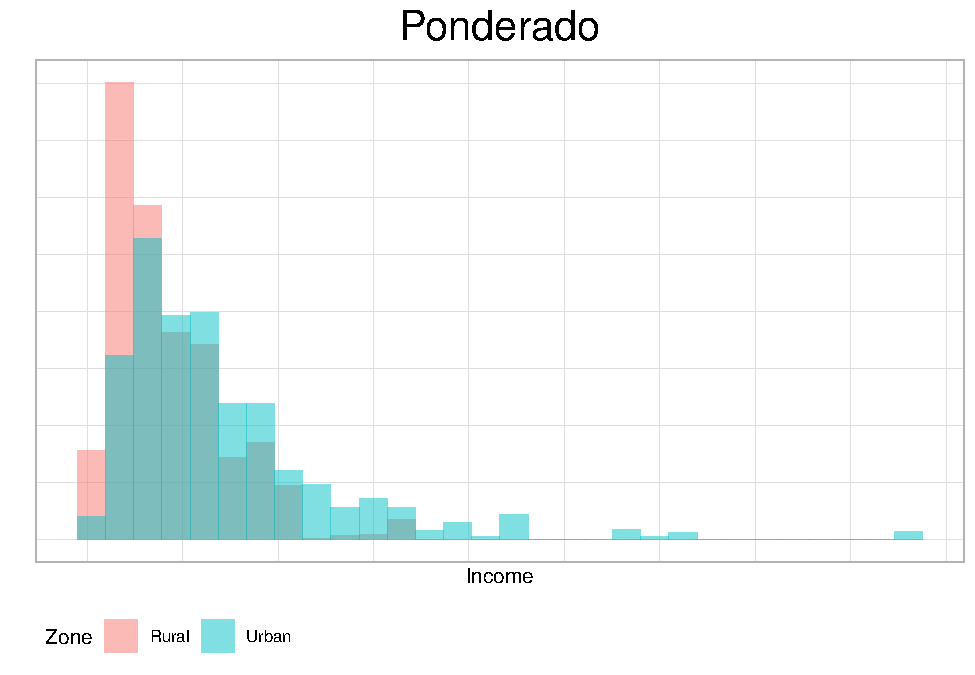
\includegraphics{07-Gráficas_files/figure-latex/hist3-1.pdf}

Como se pudo observar en la generación del histograma, se utilizó el parámetro position el cual permite que las barras del gráfico sean distingibles.

Ahora se graficará la misma variable pero esta vez sin los pesos de muestreo:

\begin{Shaded}
\begin{Highlighting}[]
\NormalTok{plot3\_SinPonde }\OtherTok{\textless{}{-}} \FunctionTok{ggplot}\NormalTok{(encuesta, }\FunctionTok{aes}\NormalTok{(}\AttributeTok{x =}\NormalTok{ Income)) }\SpecialCharTok{+}
  \FunctionTok{geom\_histogram}\NormalTok{(}\FunctionTok{aes}\NormalTok{(}\AttributeTok{y =}\NormalTok{ ..density.., }\AttributeTok{fill =}\NormalTok{ Zone),}
    \AttributeTok{alpha =} \FloatTok{0.5}\NormalTok{, }\AttributeTok{position =} \StringTok{"identity"}
\NormalTok{  ) }\SpecialCharTok{+}
  \FunctionTok{ggtitle}\NormalTok{(}\StringTok{"Sin ponderar"}\NormalTok{) }\SpecialCharTok{+}
  \FunctionTok{theme\_cepal}\NormalTok{() }\SpecialCharTok{+}
  \FunctionTok{ylab}\NormalTok{(}\StringTok{""}\NormalTok{)}
\NormalTok{plot3\_SinPonde}
\end{Highlighting}
\end{Shaded}

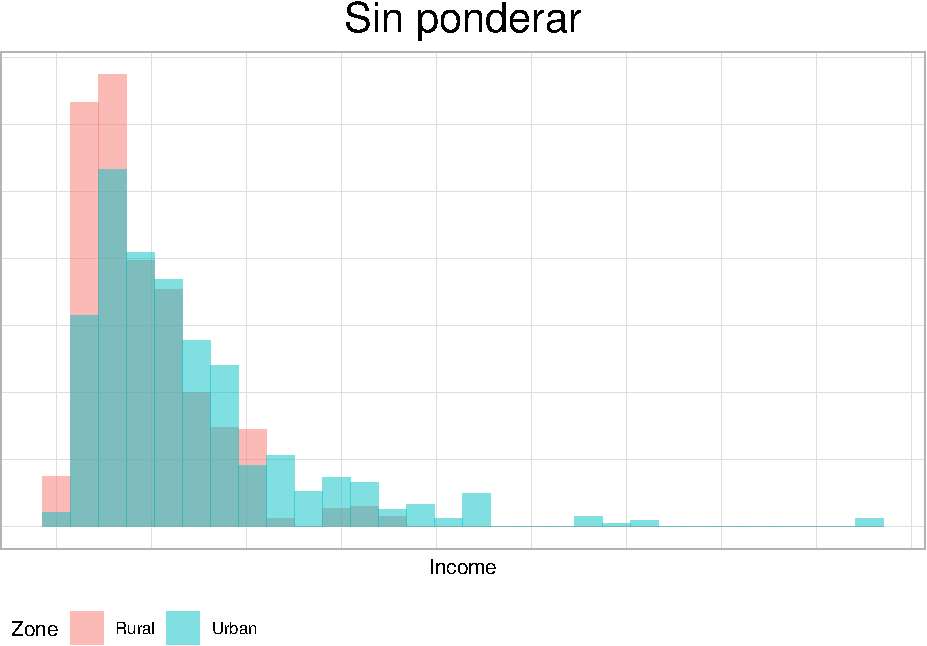
\includegraphics{07-Gráficas_files/figure-latex/hist3a-1.pdf}

Ahora, siguiendo el esquema de comparación anterior, se graficará la variable ingreso usando la información de la población y los subgrupos de zonas definidos anteriormente y por último, se muestran los 3 histogramas para poder compararlos:

\begin{Shaded}
\begin{Highlighting}[]
\NormalTok{plot3\_censo }\OtherTok{\textless{}{-}} \FunctionTok{ggplot}\NormalTok{(BigCity, }\FunctionTok{aes}\NormalTok{(}\AttributeTok{x =}\NormalTok{ Income)) }\SpecialCharTok{+}
  \FunctionTok{geom\_histogram}\NormalTok{(}\FunctionTok{aes}\NormalTok{(}\AttributeTok{y =}\NormalTok{ ..density.., }\AttributeTok{fill =}\NormalTok{ Zone),}
    \AttributeTok{alpha =} \FloatTok{0.5}\NormalTok{, }\AttributeTok{position =} \StringTok{"identity"}
\NormalTok{  ) }\SpecialCharTok{+}
  \FunctionTok{ggtitle}\NormalTok{(}\StringTok{"Poblacional"}\NormalTok{) }\SpecialCharTok{+}
  \FunctionTok{theme\_cepal}\NormalTok{() }\SpecialCharTok{+}
  \FunctionTok{xlim}\NormalTok{(}\DecValTok{0}\NormalTok{, }\DecValTok{1500}\NormalTok{) }\SpecialCharTok{+}
  \FunctionTok{ylab}\NormalTok{(}\StringTok{""}\NormalTok{)}
\NormalTok{plot3\_censo }\SpecialCharTok{|}\NormalTok{ plot3\_Ponde }\SpecialCharTok{|}\NormalTok{ plot3\_SinPonde}
\end{Highlighting}
\end{Shaded}

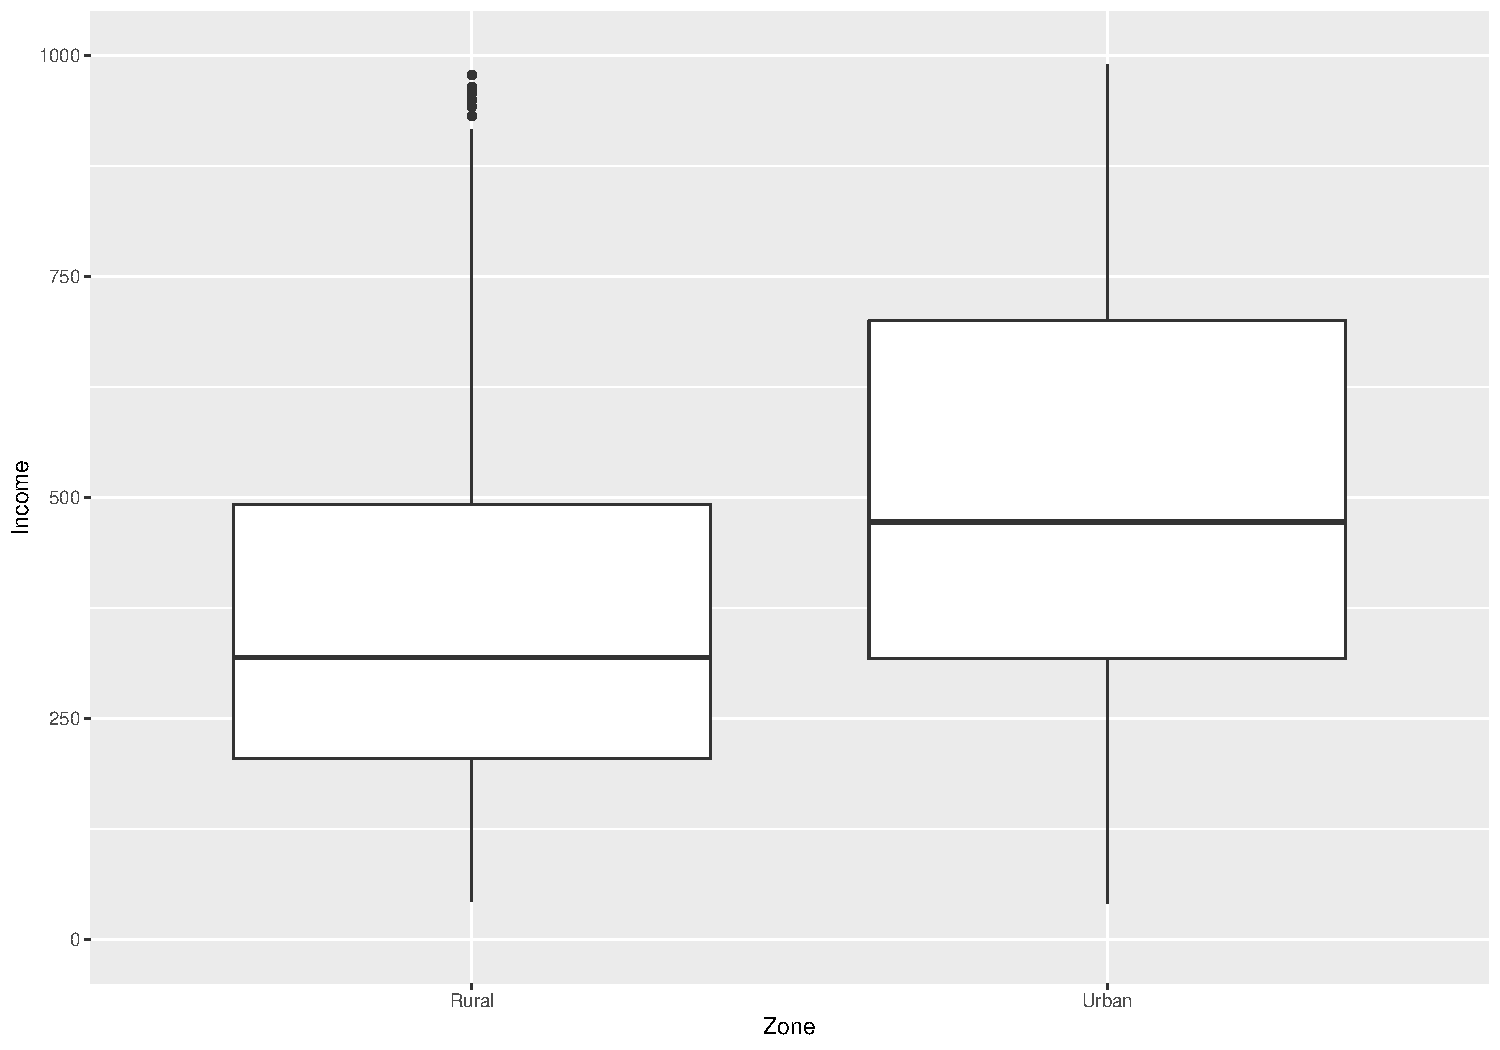
\includegraphics{07-Gráficas_files/figure-latex/unnamed-chunk-7-1.pdf}

Ahora, repetimos la secuencia de gráficos anteriores pero, para la variable \emph{Expenditure}:

\begin{Shaded}
\begin{Highlighting}[]
\NormalTok{plot4\_Ponde }\OtherTok{\textless{}{-}} \FunctionTok{ggplot}\NormalTok{(}
\NormalTok{  encuesta,}
  \FunctionTok{aes}\NormalTok{(}\AttributeTok{x =}\NormalTok{ Expenditure, }\AttributeTok{weight =}\NormalTok{ wk)}
\NormalTok{) }\SpecialCharTok{+}
  \FunctionTok{geom\_histogram}\NormalTok{(}\FunctionTok{aes}\NormalTok{(}\AttributeTok{y =}\NormalTok{ ..density.., }\AttributeTok{fill =}\NormalTok{ Zone),}
    \AttributeTok{alpha =} \FloatTok{0.5}\NormalTok{, }\AttributeTok{position =} \StringTok{"identity"}
\NormalTok{  ) }\SpecialCharTok{+}
  \FunctionTok{ylab}\NormalTok{(}\StringTok{""}\NormalTok{) }\SpecialCharTok{+}
  \FunctionTok{ggtitle}\NormalTok{(}\StringTok{"Ponderado"}\NormalTok{) }\SpecialCharTok{+}
  \FunctionTok{theme\_cepal}\NormalTok{()}
\NormalTok{plot4\_Ponde}
\end{Highlighting}
\end{Shaded}

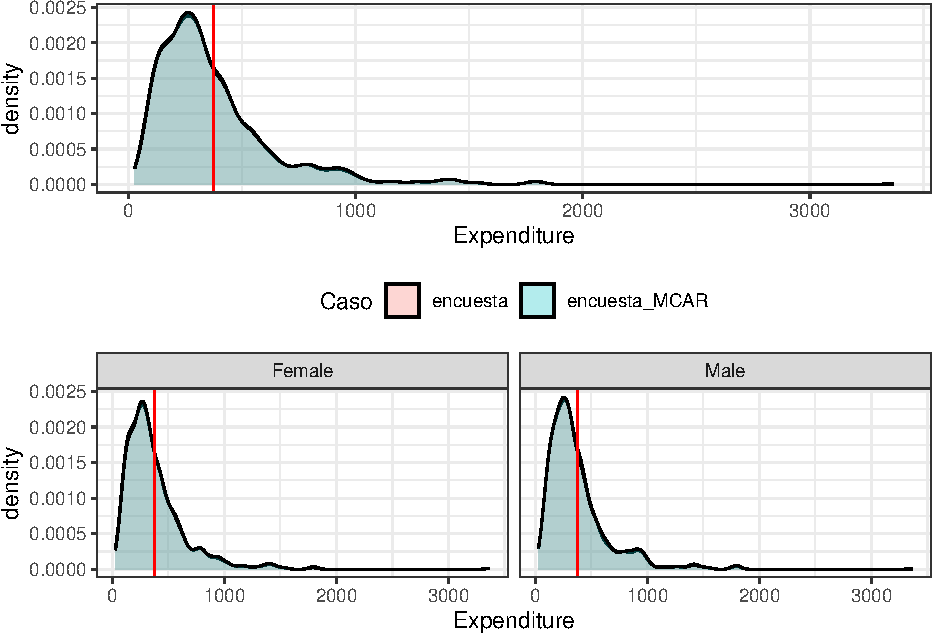
\includegraphics{07-Gráficas_files/figure-latex/unnamed-chunk-8-1.pdf}
Sin ponderar,

\begin{Shaded}
\begin{Highlighting}[]
\NormalTok{plot4\_SinPonde }\OtherTok{\textless{}{-}} \FunctionTok{ggplot}\NormalTok{(}
\NormalTok{  encuesta,}
  \FunctionTok{aes}\NormalTok{(}\AttributeTok{x =}\NormalTok{ Expenditure)}
\NormalTok{) }\SpecialCharTok{+}
  \FunctionTok{geom\_histogram}\NormalTok{(}\FunctionTok{aes}\NormalTok{(}\AttributeTok{y =}\NormalTok{ ..density.., }\AttributeTok{fill =}\NormalTok{ Zone),}
    \AttributeTok{alpha =} \FloatTok{0.5}\NormalTok{, }\AttributeTok{position =} \StringTok{"identity"}
\NormalTok{  ) }\SpecialCharTok{+}
  \FunctionTok{ggtitle}\NormalTok{(}\StringTok{"Sin ponderar"}\NormalTok{) }\SpecialCharTok{+}
  \FunctionTok{theme\_cepal}\NormalTok{() }\SpecialCharTok{+}
  \FunctionTok{ylab}\NormalTok{(}\StringTok{""}\NormalTok{)}
\NormalTok{plot4\_SinPonde}
\end{Highlighting}
\end{Shaded}

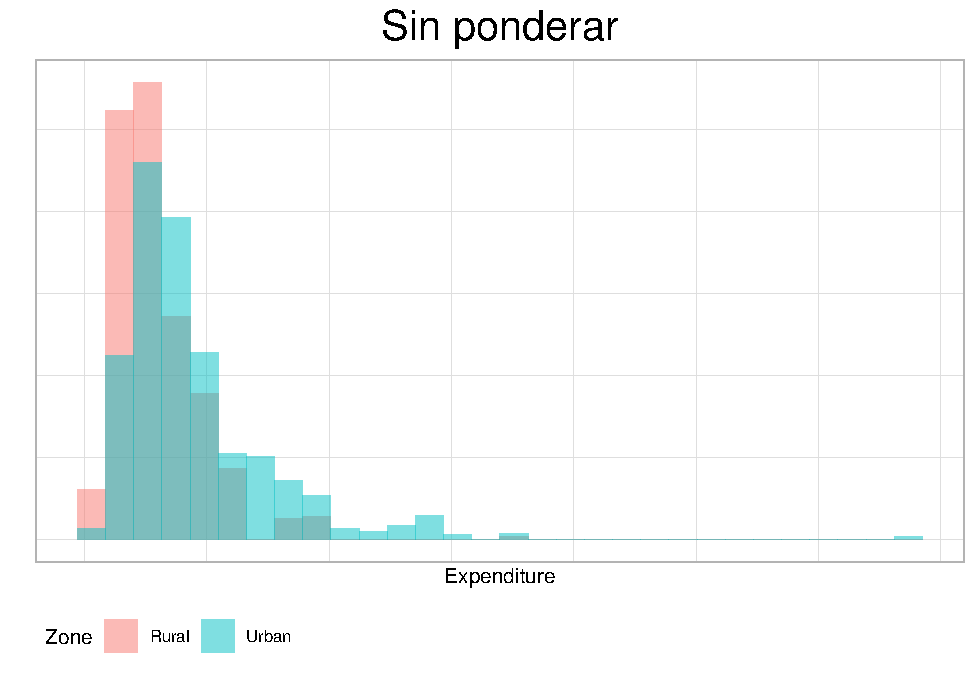
\includegraphics{07-Gráficas_files/figure-latex/unnamed-chunk-9-1.pdf}

Poblacional,

\begin{Shaded}
\begin{Highlighting}[]
\NormalTok{plot4\_censo }\OtherTok{\textless{}{-}} \FunctionTok{ggplot}\NormalTok{(BigCity, }\FunctionTok{aes}\NormalTok{(}\AttributeTok{x =}\NormalTok{ Expenditure)) }\SpecialCharTok{+}
  \FunctionTok{geom\_histogram}\NormalTok{(}\FunctionTok{aes}\NormalTok{(}\AttributeTok{y =}\NormalTok{ ..density.., }\AttributeTok{fill =}\NormalTok{ Zone),}
    \AttributeTok{alpha =} \FloatTok{0.5}\NormalTok{, }\AttributeTok{position =} \StringTok{"identity"}
\NormalTok{  ) }\SpecialCharTok{+}
  \FunctionTok{ggtitle}\NormalTok{(}\StringTok{"Poblacional"}\NormalTok{) }\SpecialCharTok{+}
  \FunctionTok{theme\_cepal}\NormalTok{() }\SpecialCharTok{+}
  \FunctionTok{xlim}\NormalTok{(}\DecValTok{0}\NormalTok{, }\DecValTok{1500}\NormalTok{) }\SpecialCharTok{+}
  \FunctionTok{ylab}\NormalTok{(}\StringTok{""}\NormalTok{)}
\NormalTok{plot4\_censo }\SpecialCharTok{|}\NormalTok{ plot4\_Ponde }\SpecialCharTok{|}\NormalTok{ plot4\_SinPonde}
\end{Highlighting}
\end{Shaded}

Ahora, repetimos la secuencia de gráficos para la variable \emph{Income}, pero hacemos las particiones por la variable \emph{sexo}, Primero, hagamos el histogramas ponderado:

\begin{Shaded}
\begin{Highlighting}[]
\NormalTok{plot5\_Ponde }\OtherTok{\textless{}{-}} \FunctionTok{ggplot}\NormalTok{(}
\NormalTok{  encuesta,}
  \FunctionTok{aes}\NormalTok{(}\AttributeTok{x =}\NormalTok{ Income, }\AttributeTok{weight =}\NormalTok{ wk)}
\NormalTok{) }\SpecialCharTok{+}
  \FunctionTok{geom\_histogram}\NormalTok{(}\FunctionTok{aes}\NormalTok{(}\AttributeTok{y =}\NormalTok{ ..density.., }\AttributeTok{fill =}\NormalTok{ Sex),}
    \AttributeTok{alpha =} \FloatTok{0.5}\NormalTok{, }\AttributeTok{position =} \StringTok{"identity"}
\NormalTok{  ) }\SpecialCharTok{+}
  \FunctionTok{ylab}\NormalTok{(}\StringTok{""}\NormalTok{) }\SpecialCharTok{+}
  \FunctionTok{ggtitle}\NormalTok{(}\StringTok{"Ponderado"}\NormalTok{) }\SpecialCharTok{+}
  \FunctionTok{theme\_cepal}\NormalTok{()}
\NormalTok{plot5\_Ponde}
\end{Highlighting}
\end{Shaded}

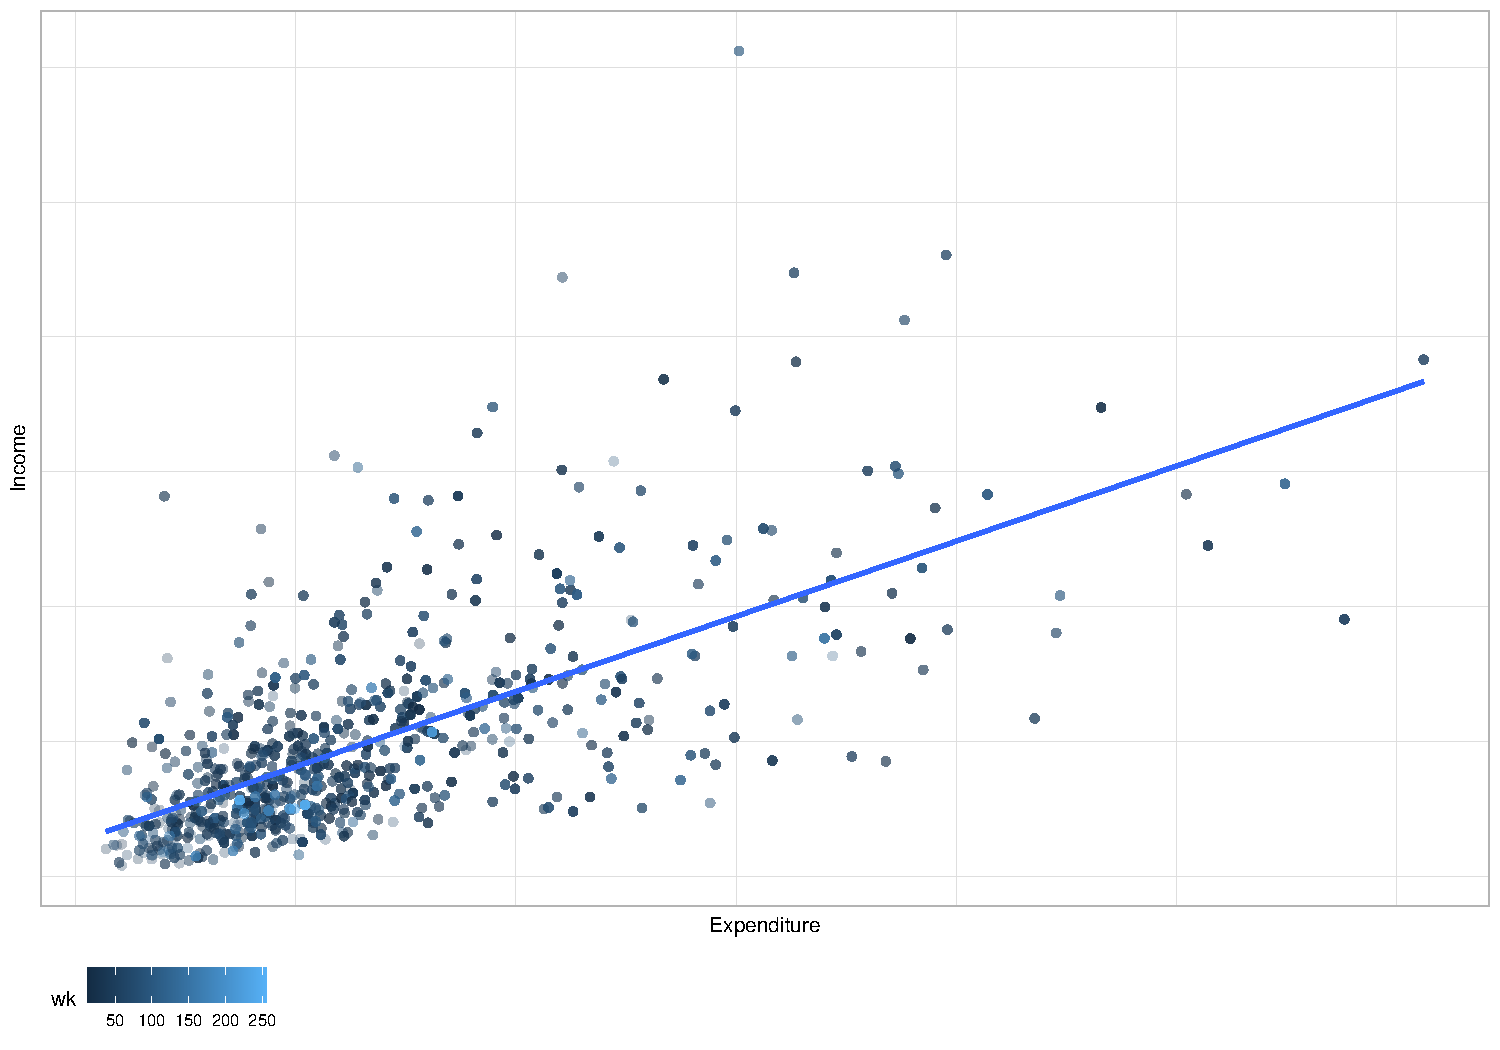
\includegraphics{07-Gráficas_files/figure-latex/unnamed-chunk-11-1.pdf}

Sin ponderar,

\begin{Shaded}
\begin{Highlighting}[]
\NormalTok{plot5\_SinPonde }\OtherTok{\textless{}{-}} \FunctionTok{ggplot}\NormalTok{(encuesta, }\FunctionTok{aes}\NormalTok{(}\AttributeTok{x =}\NormalTok{ Income)) }\SpecialCharTok{+}
  \FunctionTok{geom\_histogram}\NormalTok{(}\FunctionTok{aes}\NormalTok{(}\AttributeTok{y =}\NormalTok{ ..density.., }\AttributeTok{fill =}\NormalTok{ Sex),}
    \AttributeTok{alpha =} \FloatTok{0.5}\NormalTok{, }\AttributeTok{position =} \StringTok{"identity"}
\NormalTok{  ) }\SpecialCharTok{+}
  \FunctionTok{ggtitle}\NormalTok{(}\StringTok{"Sin ponderar"}\NormalTok{) }\SpecialCharTok{+}
  \FunctionTok{theme\_cepal}\NormalTok{() }\SpecialCharTok{+}
  \FunctionTok{ylab}\NormalTok{(}\StringTok{""}\NormalTok{)}
\NormalTok{plot5\_SinPonde}
\end{Highlighting}
\end{Shaded}

\includegraphics{07-Gráficas_files/figure-latex/unnamed-chunk-12-1.pdf}

Poblacional,

\begin{Shaded}
\begin{Highlighting}[]
\NormalTok{plot5\_censo }\OtherTok{\textless{}{-}} \FunctionTok{ggplot}\NormalTok{(BigCity, }\FunctionTok{aes}\NormalTok{(}\AttributeTok{x =}\NormalTok{ Income)) }\SpecialCharTok{+}
  \FunctionTok{geom\_histogram}\NormalTok{(}\FunctionTok{aes}\NormalTok{(}\AttributeTok{y =}\NormalTok{ ..density.., }\AttributeTok{fill =}\NormalTok{ Sex),}
    \AttributeTok{alpha =} \FloatTok{0.5}\NormalTok{, }\AttributeTok{position =} \StringTok{"identity"}
\NormalTok{  ) }\SpecialCharTok{+}
  \FunctionTok{ggtitle}\NormalTok{(}\StringTok{"Poblacional"}\NormalTok{) }\SpecialCharTok{+}
  \FunctionTok{theme\_cepal}\NormalTok{() }\SpecialCharTok{+}
  \FunctionTok{xlim}\NormalTok{(}\DecValTok{0}\NormalTok{, }\DecValTok{1500}\NormalTok{) }\SpecialCharTok{+}
  \FunctionTok{ylab}\NormalTok{(}\StringTok{""}\NormalTok{)}
\NormalTok{plot5\_censo }\SpecialCharTok{|}\NormalTok{ plot5\_Ponde }\SpecialCharTok{|}\NormalTok{ plot5\_SinPonde}
\end{Highlighting}
\end{Shaded}

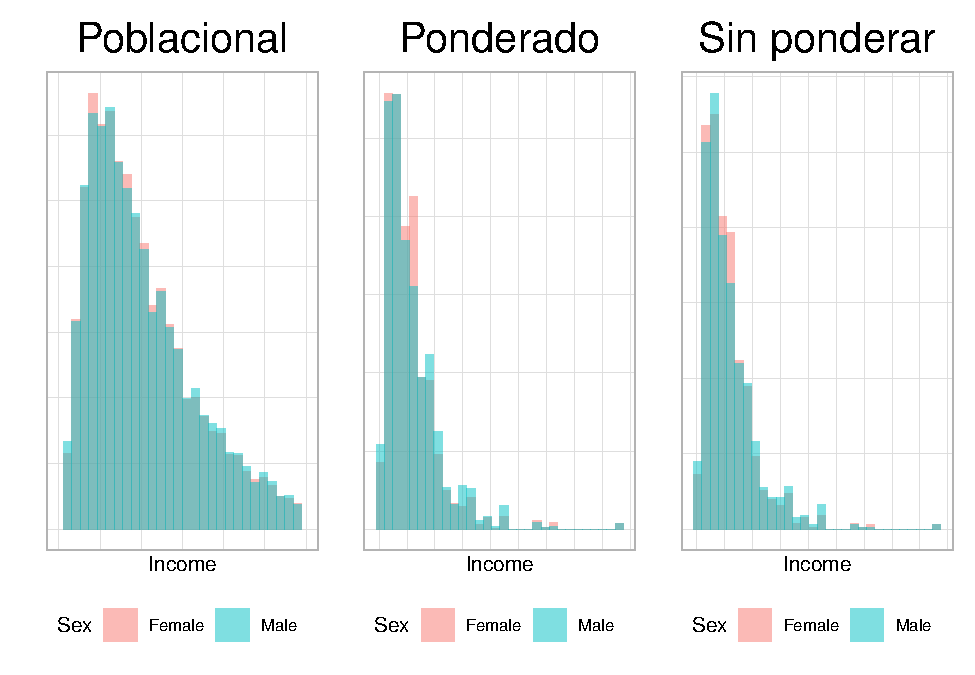
\includegraphics{07-Gráficas_files/figure-latex/unnamed-chunk-13-1.pdf}

Ahora, repetimos la secuencia de gráficos para la variable \emph{Expenditure} desagregada por la variable \emph{sexo}, primero, ponderado:

\begin{Shaded}
\begin{Highlighting}[]
\NormalTok{plot6\_Ponde }\OtherTok{\textless{}{-}} \FunctionTok{ggplot}\NormalTok{(}
\NormalTok{  encuesta,}
  \FunctionTok{aes}\NormalTok{(}\AttributeTok{x =}\NormalTok{ Expenditure, }\AttributeTok{weight =}\NormalTok{ wk)}
\NormalTok{) }\SpecialCharTok{+}
  \FunctionTok{geom\_histogram}\NormalTok{(}\FunctionTok{aes}\NormalTok{(}\AttributeTok{y =}\NormalTok{ ..density.., }\AttributeTok{fill =}\NormalTok{ Sex),}
    \AttributeTok{alpha =} \FloatTok{0.5}\NormalTok{, }\AttributeTok{position =} \StringTok{"identity"}
\NormalTok{  ) }\SpecialCharTok{+}
  \FunctionTok{ylab}\NormalTok{(}\StringTok{""}\NormalTok{) }\SpecialCharTok{+}
  \FunctionTok{ggtitle}\NormalTok{(}\StringTok{"Ponderado"}\NormalTok{) }\SpecialCharTok{+}
  \FunctionTok{theme\_cepal}\NormalTok{()}
\NormalTok{plot6\_Ponde}
\end{Highlighting}
\end{Shaded}

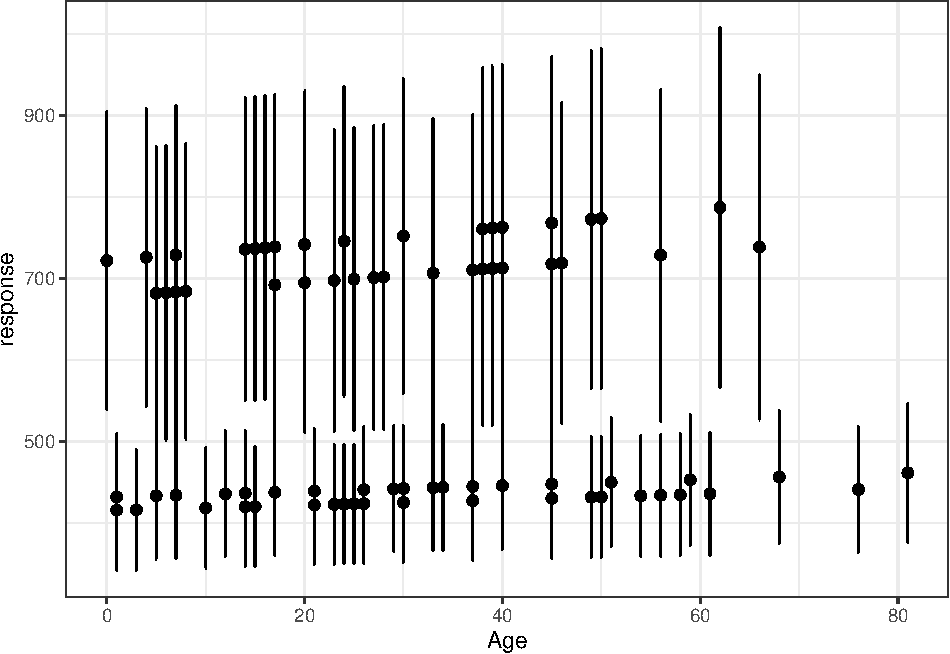
\includegraphics{07-Gráficas_files/figure-latex/unnamed-chunk-14-1.pdf}

Sin ponderar,

\begin{Shaded}
\begin{Highlighting}[]
\NormalTok{plot6\_SinPonde }\OtherTok{\textless{}{-}} \FunctionTok{ggplot}\NormalTok{(encuesta, }\FunctionTok{aes}\NormalTok{(}\AttributeTok{x =}\NormalTok{ Expenditure)) }\SpecialCharTok{+}
  \FunctionTok{geom\_histogram}\NormalTok{(}\FunctionTok{aes}\NormalTok{(}\AttributeTok{y =}\NormalTok{ ..density.., }\AttributeTok{fill =}\NormalTok{ Sex),}
    \AttributeTok{alpha =} \FloatTok{0.5}\NormalTok{, }\AttributeTok{position =} \StringTok{"identity"}
\NormalTok{  ) }\SpecialCharTok{+}
  \FunctionTok{ggtitle}\NormalTok{(}\StringTok{"Sin ponderar"}\NormalTok{) }\SpecialCharTok{+}
  \FunctionTok{theme\_cepal}\NormalTok{() }\SpecialCharTok{+}
  \FunctionTok{ylab}\NormalTok{(}\StringTok{""}\NormalTok{)}
\NormalTok{plot6\_SinPonde}
\end{Highlighting}
\end{Shaded}

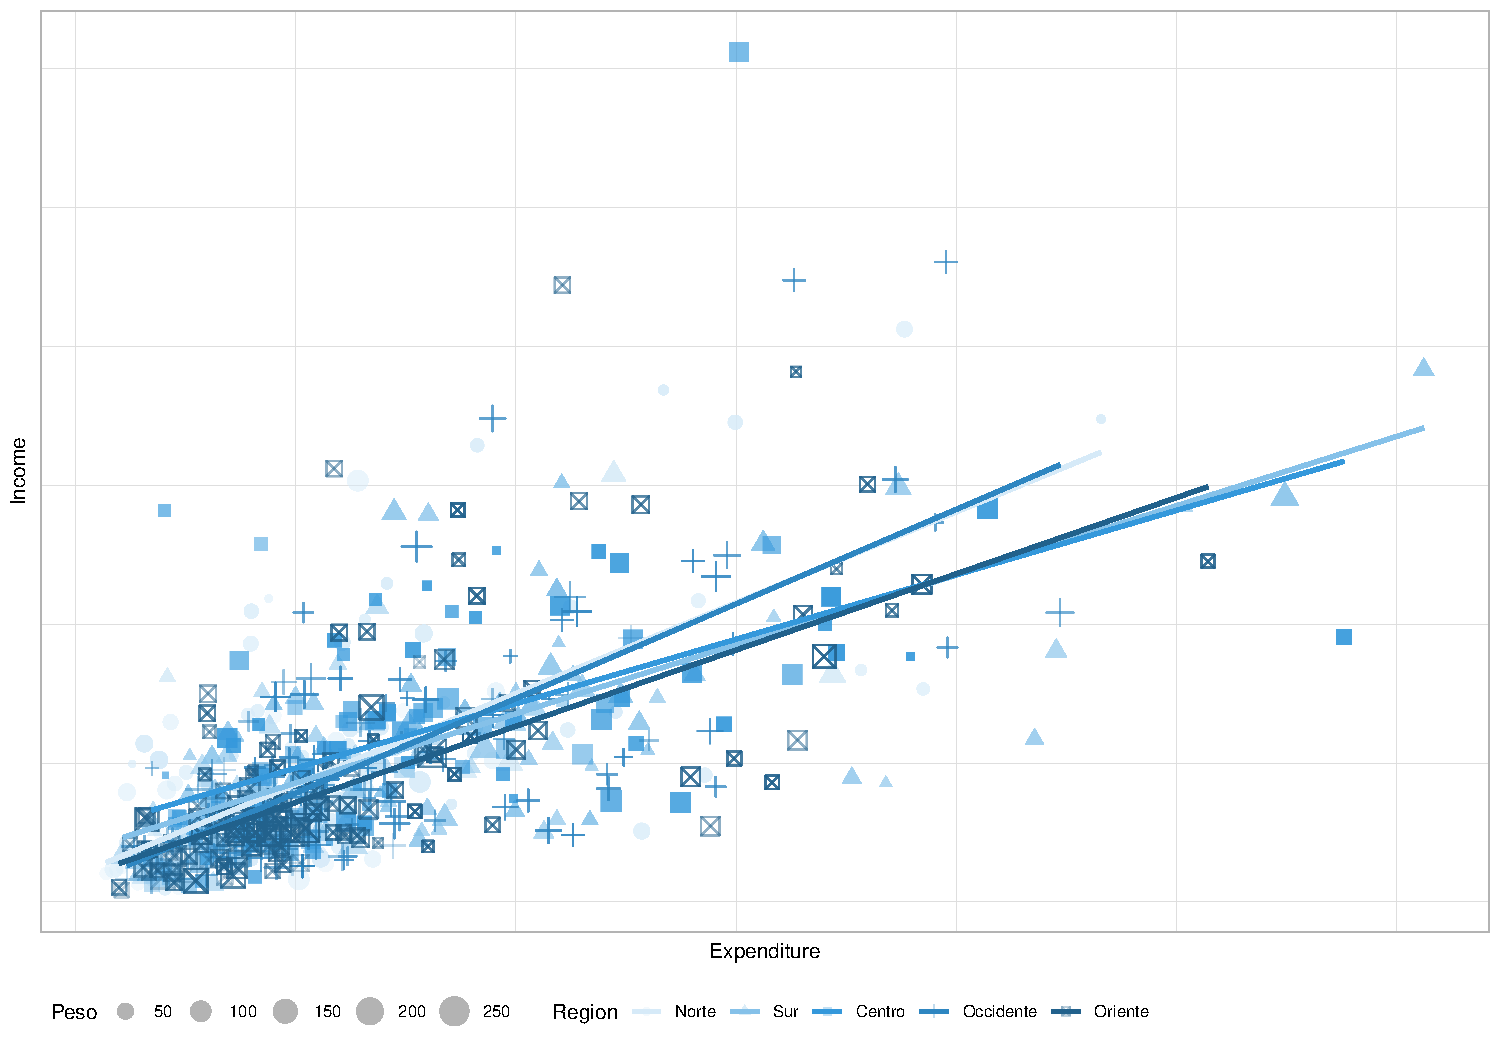
\includegraphics{07-Gráficas_files/figure-latex/unnamed-chunk-15-1.pdf}

Poblacional,

\begin{Shaded}
\begin{Highlighting}[]
\NormalTok{plot6\_censo }\OtherTok{\textless{}{-}} \FunctionTok{ggplot}\NormalTok{(BigCity, }\FunctionTok{aes}\NormalTok{(}\AttributeTok{x =}\NormalTok{ Expenditure)) }\SpecialCharTok{+}
  \FunctionTok{geom\_histogram}\NormalTok{(}\FunctionTok{aes}\NormalTok{(}\AttributeTok{y =}\NormalTok{ ..density.., }\AttributeTok{fill =}\NormalTok{ Sex),}
    \AttributeTok{alpha =} \FloatTok{0.5}\NormalTok{, }\AttributeTok{position =} \StringTok{"identity"}
\NormalTok{  ) }\SpecialCharTok{+}
  \FunctionTok{ggtitle}\NormalTok{(}\StringTok{"Poblacional"}\NormalTok{) }\SpecialCharTok{+}
  \FunctionTok{theme\_cepal}\NormalTok{() }\SpecialCharTok{+}
  \FunctionTok{xlim}\NormalTok{(}\DecValTok{0}\NormalTok{, }\DecValTok{1500}\NormalTok{) }\SpecialCharTok{+}
  \FunctionTok{ylab}\NormalTok{(}\StringTok{""}\NormalTok{)}
\NormalTok{plot6\_censo }\SpecialCharTok{|}\NormalTok{ plot6\_Ponde }\SpecialCharTok{|}\NormalTok{ plot6\_SinPonde}
\end{Highlighting}
\end{Shaded}

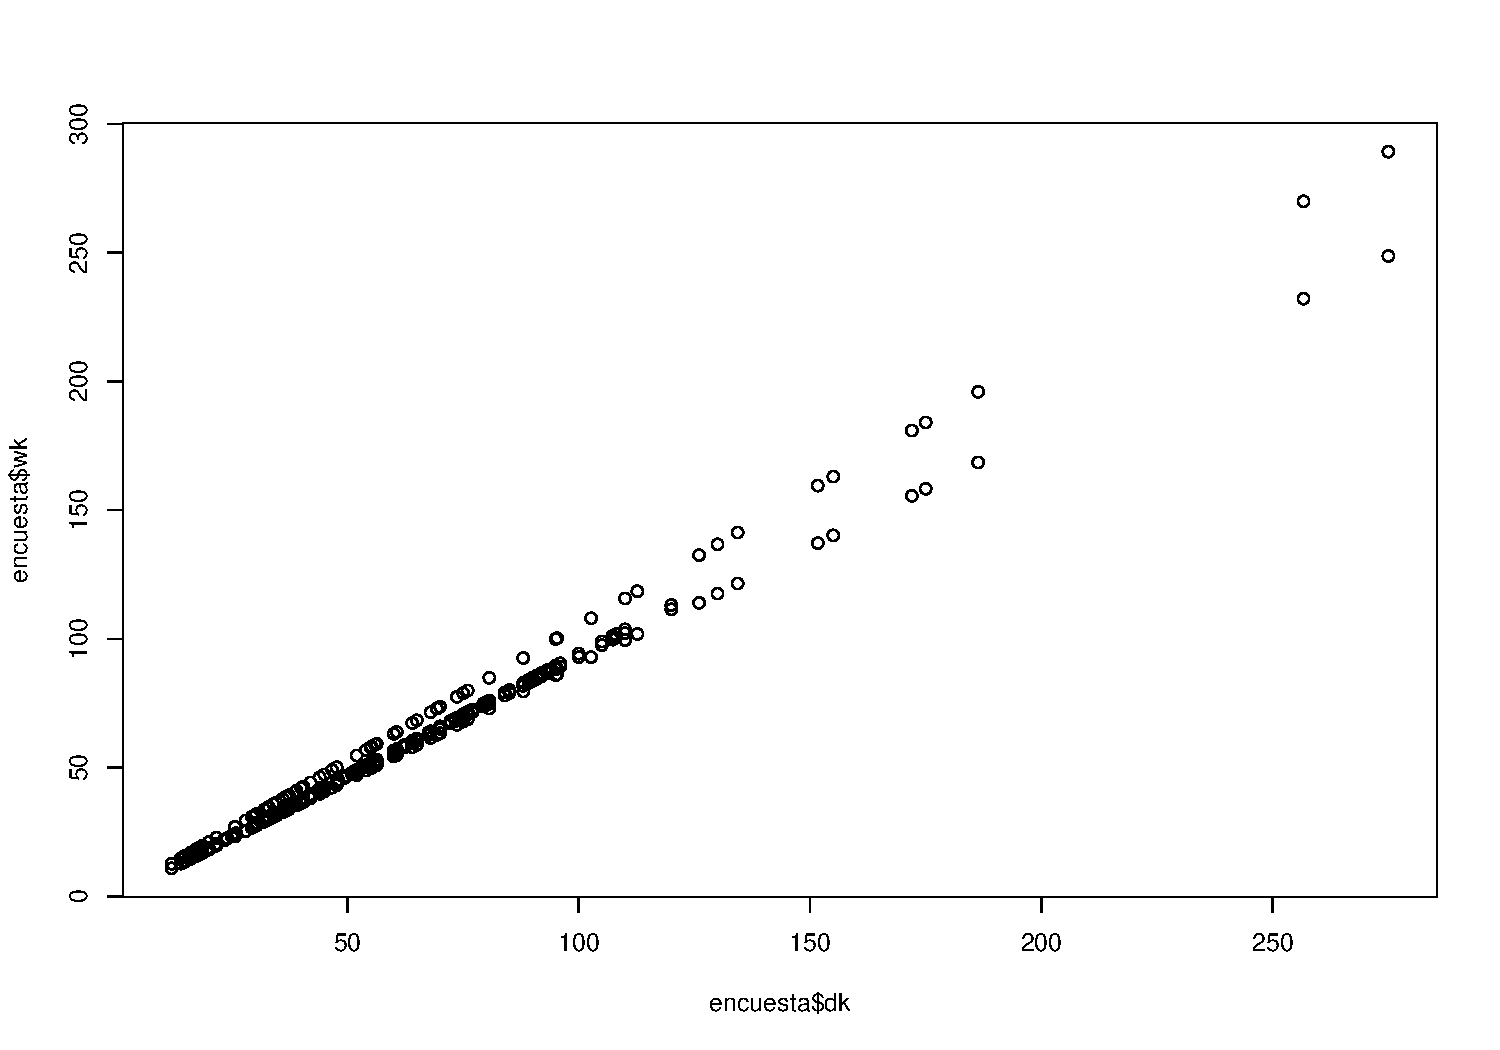
\includegraphics{07-Gráficas_files/figure-latex/unnamed-chunk-16-1.pdf}

\hypertarget{agregando-densidades-y-graficando-boxplot}{%
\section{Agregando densidades y graficando Boxplot}\label{agregando-densidades-y-graficando-boxplot}}

Dadas las cualidades de la librería ggplot2, se pueden agregar nuevas capas a los gráficos, particularmente, a los histogramas antes realizados. La densidad se agrega con el argumento \texttt{geom\_density} y se incorpora el parámetro \texttt{alpha} que regula la transparencia del relleno. A continuacuón, se muestra cómo se agregan las densidades:

\begin{Shaded}
\begin{Highlighting}[]
\NormalTok{plot1\_Ponde }\SpecialCharTok{+} \FunctionTok{geom\_density}\NormalTok{(}\AttributeTok{fill =} \StringTok{"blue"}\NormalTok{, }\AttributeTok{alpha =} \FloatTok{0.3}\NormalTok{) }\SpecialCharTok{|}
\NormalTok{  plot2\_Ponde }\SpecialCharTok{+} \FunctionTok{geom\_density}\NormalTok{(}\AttributeTok{fill =} \StringTok{"blue"}\NormalTok{, }\AttributeTok{alpha =} \FloatTok{0.3}\NormalTok{)}
\end{Highlighting}
\end{Shaded}

\begin{center}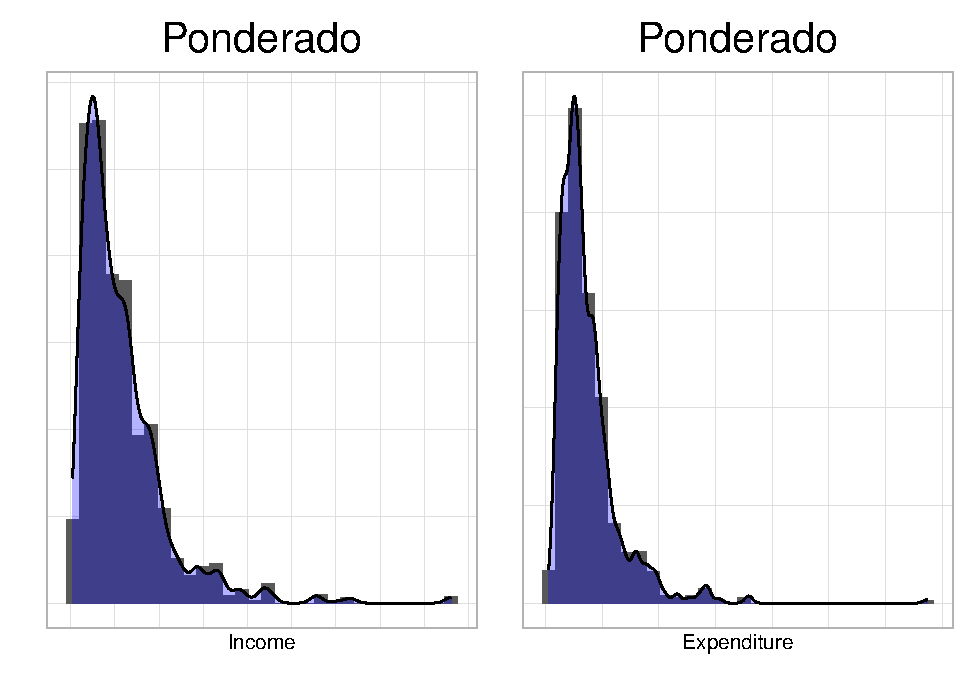
\includegraphics[width=0.6\linewidth]{07-Gráficas_files/figure-latex/unnamed-chunk-17-1} \end{center}

Ahora bien, al aplicar \texttt{aes(fill\ =\ Zone)} permite que la densidad sea agregada para cada una de las agrupaciones como se muestra a continución,

\begin{Shaded}
\begin{Highlighting}[]
\NormalTok{plot3\_Ponde }\SpecialCharTok{+} \FunctionTok{geom\_density}\NormalTok{(}\FunctionTok{aes}\NormalTok{(}\AttributeTok{fill =}\NormalTok{ Zone), }\AttributeTok{alpha =} \FloatTok{0.3}\NormalTok{) }\SpecialCharTok{|}
\NormalTok{  plot4\_Ponde }\SpecialCharTok{+} \FunctionTok{geom\_density}\NormalTok{(}\FunctionTok{aes}\NormalTok{(}\AttributeTok{fill =}\NormalTok{ Zone), }\AttributeTok{alpha =} \FloatTok{0.3}\NormalTok{)}
\end{Highlighting}
\end{Shaded}

\begin{center}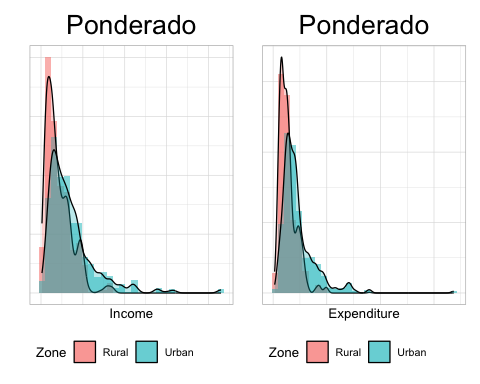
\includegraphics[width=0.6\linewidth]{07-Gráficas_files/figure-latex/unnamed-chunk-18-1} \end{center}

En está oportunidad se agrega la desnidad por sexo,

\begin{Shaded}
\begin{Highlighting}[]
\NormalTok{plot5\_Ponde }\SpecialCharTok{+} \FunctionTok{geom\_density}\NormalTok{(}\FunctionTok{aes}\NormalTok{(}\AttributeTok{fill =}\NormalTok{ Sex), }\AttributeTok{alpha =} \FloatTok{0.3}\NormalTok{) }\SpecialCharTok{|}
\NormalTok{  plot6\_Ponde }\SpecialCharTok{+} \FunctionTok{geom\_density}\NormalTok{(}\FunctionTok{aes}\NormalTok{(}\AttributeTok{fill =}\NormalTok{ Sex), }\AttributeTok{alpha =} \FloatTok{0.3}\NormalTok{)}
\end{Highlighting}
\end{Shaded}

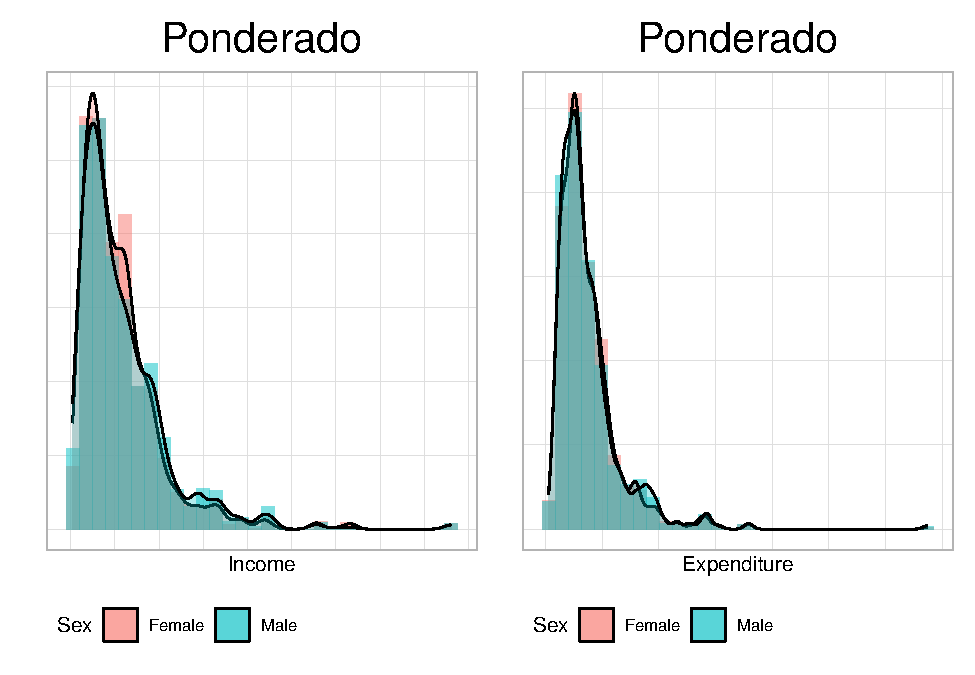
\includegraphics{07-Gráficas_files/figure-latex/unnamed-chunk-19-1.pdf}

\emph{Boxplot}

El boxplot, diagrama de caja y bigotes, es un gráfico resumen presentado por John Tukey en 1977 que en la actualidad es ampliamente utilizado en la práctica estadística. En este diagrama se visualiza de forma general un conjunto de datos empleando el resumen de cinco números. La forma generada por este gráfico compuesto por un rectángulo (``caja'') y dos brazos (``bigotes'') suministra información sobre la relación ente los cuartiles (Q1, Q2 o mediana y Q3) y los valores mínimo y máximo, sobre la existencia de valores atípicos y la simetría
de la distribución.

Para realizar este gráfico en ggplot2 se utiliza la función \texttt{geom\_boxplot}. A continuación, se presentan los Boxplot para las variables ingresos y gastos respectivamente:

\begin{Shaded}
\begin{Highlighting}[]
\NormalTok{plot7\_Ponde }\OtherTok{\textless{}{-}} \FunctionTok{ggplot}\NormalTok{(}
  \AttributeTok{data =}\NormalTok{ encuesta, }\FunctionTok{aes}\NormalTok{(}\AttributeTok{x =}\NormalTok{ Income, }\AttributeTok{weight =}\NormalTok{ wk)}
\NormalTok{) }\SpecialCharTok{+}
  \FunctionTok{geom\_boxplot}\NormalTok{() }\SpecialCharTok{+}
  \FunctionTok{ggtitle}\NormalTok{(}\StringTok{"Ponderado"}\NormalTok{) }\SpecialCharTok{+}
  \FunctionTok{coord\_flip}\NormalTok{() }\SpecialCharTok{+}
  \FunctionTok{theme\_cepal}\NormalTok{()}


\NormalTok{plot8\_Ponde }\OtherTok{\textless{}{-}} \FunctionTok{ggplot}\NormalTok{(}
\NormalTok{  encuesta,}
  \FunctionTok{aes}\NormalTok{(}\AttributeTok{x =}\NormalTok{ Expenditure, }\AttributeTok{weight =}\NormalTok{ wk)}
\NormalTok{) }\SpecialCharTok{+}
  \FunctionTok{geom\_boxplot}\NormalTok{() }\SpecialCharTok{+}
  \FunctionTok{ggtitle}\NormalTok{(}\StringTok{"Ponderado"}\NormalTok{) }\SpecialCharTok{+}
  \FunctionTok{coord\_flip}\NormalTok{() }\SpecialCharTok{+}
  \FunctionTok{theme\_cepal}\NormalTok{()}

\NormalTok{plot7\_Ponde }\SpecialCharTok{|}\NormalTok{ plot8\_Ponde}
\end{Highlighting}
\end{Shaded}

En los gráficos anteriores se puede observar que la variable ingresos tiene más variabilidad que la variable gastos. En ambos gráficos se observan datos atípicos.

Estos diagramas también permiten la comparación entre dos o más niveles de agrupamiento, por ejemplo, por zonas para las variables ingresos y gastos como se muestra a continuación,

\begin{Shaded}
\begin{Highlighting}[]
\NormalTok{plot9\_Ponde }\OtherTok{\textless{}{-}} \FunctionTok{ggplot}\NormalTok{(}
\NormalTok{  encuesta,}
  \FunctionTok{aes}\NormalTok{(}\AttributeTok{x =}\NormalTok{ Income, }\AttributeTok{weight =}\NormalTok{ wk)}
\NormalTok{) }\SpecialCharTok{+}
  \FunctionTok{geom\_boxplot}\NormalTok{(}\FunctionTok{aes}\NormalTok{(}\AttributeTok{fill =}\NormalTok{ Zone)) }\SpecialCharTok{+}
  \FunctionTok{ggtitle}\NormalTok{(}\StringTok{"Ponderado"}\NormalTok{) }\SpecialCharTok{+}
  \FunctionTok{coord\_flip}\NormalTok{() }\SpecialCharTok{+}
  \FunctionTok{theme\_cepal}\NormalTok{()}

\NormalTok{plot10\_Ponde }\OtherTok{\textless{}{-}} \FunctionTok{ggplot}\NormalTok{(}
\NormalTok{  encuesta,}
  \FunctionTok{aes}\NormalTok{(}\AttributeTok{x =}\NormalTok{ Expenditure, }\AttributeTok{weight =}\NormalTok{ wk)}
\NormalTok{) }\SpecialCharTok{+}
  \FunctionTok{geom\_boxplot}\NormalTok{(}\FunctionTok{aes}\NormalTok{(}\AttributeTok{fill =}\NormalTok{ Zone)) }\SpecialCharTok{+}
  \FunctionTok{ggtitle}\NormalTok{(}\StringTok{"Ponderado"}\NormalTok{) }\SpecialCharTok{+}
  \FunctionTok{coord\_flip}\NormalTok{() }\SpecialCharTok{+}
  \FunctionTok{theme\_cepal}\NormalTok{()}

\NormalTok{plot9\_Ponde }\SpecialCharTok{|}\NormalTok{ plot10\_Ponde}
\end{Highlighting}
\end{Shaded}

\includegraphics{07-Gráficas_files/figure-latex/unnamed-chunk-21-1.pdf}
Observándose, entre otros que, para la variable gasto en la zona rural es donde más datos atípico hay.

Ahora, si se desea personalizar los colores del relleno debe hacer uso de la función \texttt{scale\_fill\_manual}como se muestra a continuación:

\begin{Shaded}
\begin{Highlighting}[]
\NormalTok{colorZona }\OtherTok{\textless{}{-}} \FunctionTok{c}\NormalTok{(}\AttributeTok{Urban =} \StringTok{"\#48C9B0"}\NormalTok{, }\AttributeTok{Rural =} \StringTok{"\#117864"}\NormalTok{)}
\NormalTok{plot9\_Ponde }\SpecialCharTok{+} \FunctionTok{scale\_fill\_manual}\NormalTok{(}\AttributeTok{values =}\NormalTok{ colorZona) }\SpecialCharTok{|}
\NormalTok{  plot10\_Ponde }\SpecialCharTok{+} \FunctionTok{scale\_fill\_manual}\NormalTok{(}\AttributeTok{values =}\NormalTok{ colorZona)}
\end{Highlighting}
\end{Shaded}

\begin{center}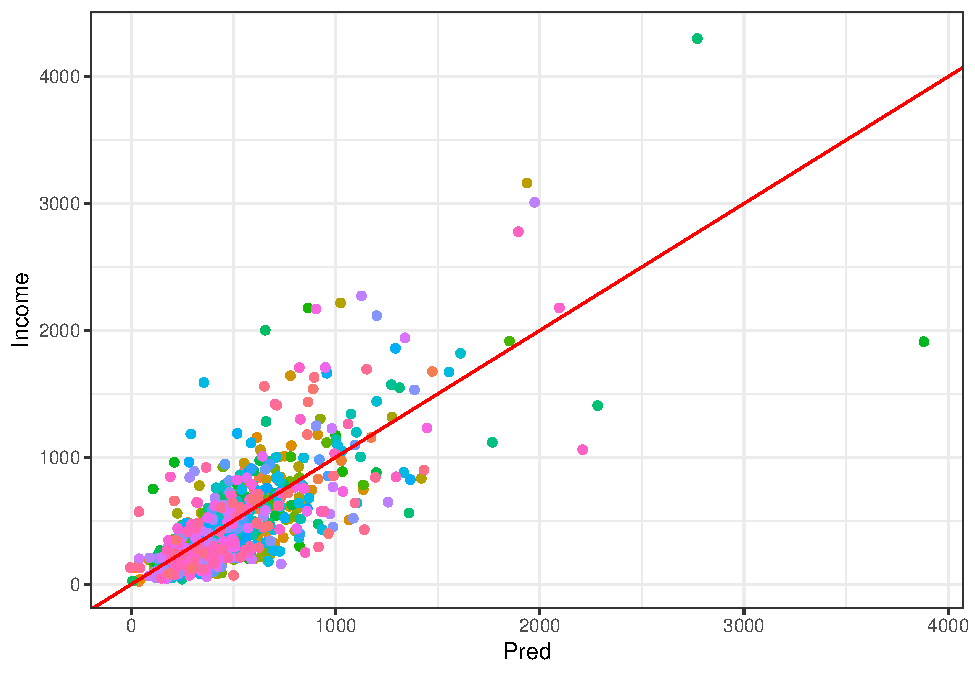
\includegraphics[width=0.6\linewidth]{07-Gráficas_files/figure-latex/unnamed-chunk-22-1} \end{center}

Para mayores colores, ver la ayuda de la librería. Ahora, si se desea comparar los ingresos y gastos por sexo se procede de la siguiente manera:

\begin{Shaded}
\begin{Highlighting}[]
\NormalTok{plot11\_Ponde }\OtherTok{\textless{}{-}} \FunctionTok{ggplot}\NormalTok{(}
  \AttributeTok{data =}\NormalTok{ encuesta,}
  \FunctionTok{aes}\NormalTok{(}\AttributeTok{x =}\NormalTok{ Income, }\AttributeTok{weight =}\NormalTok{ wk)) }\SpecialCharTok{+}
  \FunctionTok{geom\_boxplot}\NormalTok{(}\FunctionTok{aes}\NormalTok{(}\AttributeTok{fill =}\NormalTok{ Sex)) }\SpecialCharTok{+}
  \FunctionTok{ggtitle}\NormalTok{(}\StringTok{"Ponderado"}\NormalTok{) }\SpecialCharTok{+}
  \FunctionTok{coord\_flip}\NormalTok{() }\SpecialCharTok{+}
  \FunctionTok{theme\_cepal}\NormalTok{()}

\NormalTok{plot12\_Ponde }\OtherTok{\textless{}{-}} \FunctionTok{ggplot}\NormalTok{(}
\NormalTok{  encuesta,}
  \FunctionTok{aes}\NormalTok{(}\AttributeTok{x =}\NormalTok{ Expenditure, }\AttributeTok{weight =}\NormalTok{ wk)}
\NormalTok{) }\SpecialCharTok{+}
  \FunctionTok{geom\_boxplot}\NormalTok{(}\FunctionTok{aes}\NormalTok{(}\AttributeTok{fill =}\NormalTok{ Sex)) }\SpecialCharTok{+}
  \FunctionTok{ggtitle}\NormalTok{(}\StringTok{"Ponderado"}\NormalTok{) }\SpecialCharTok{+}
  \FunctionTok{coord\_flip}\NormalTok{() }\SpecialCharTok{+}
  \FunctionTok{theme\_cepal}\NormalTok{()}

\NormalTok{plot11\_Ponde }\SpecialCharTok{|}\NormalTok{ plot12\_Ponde}
\end{Highlighting}
\end{Shaded}

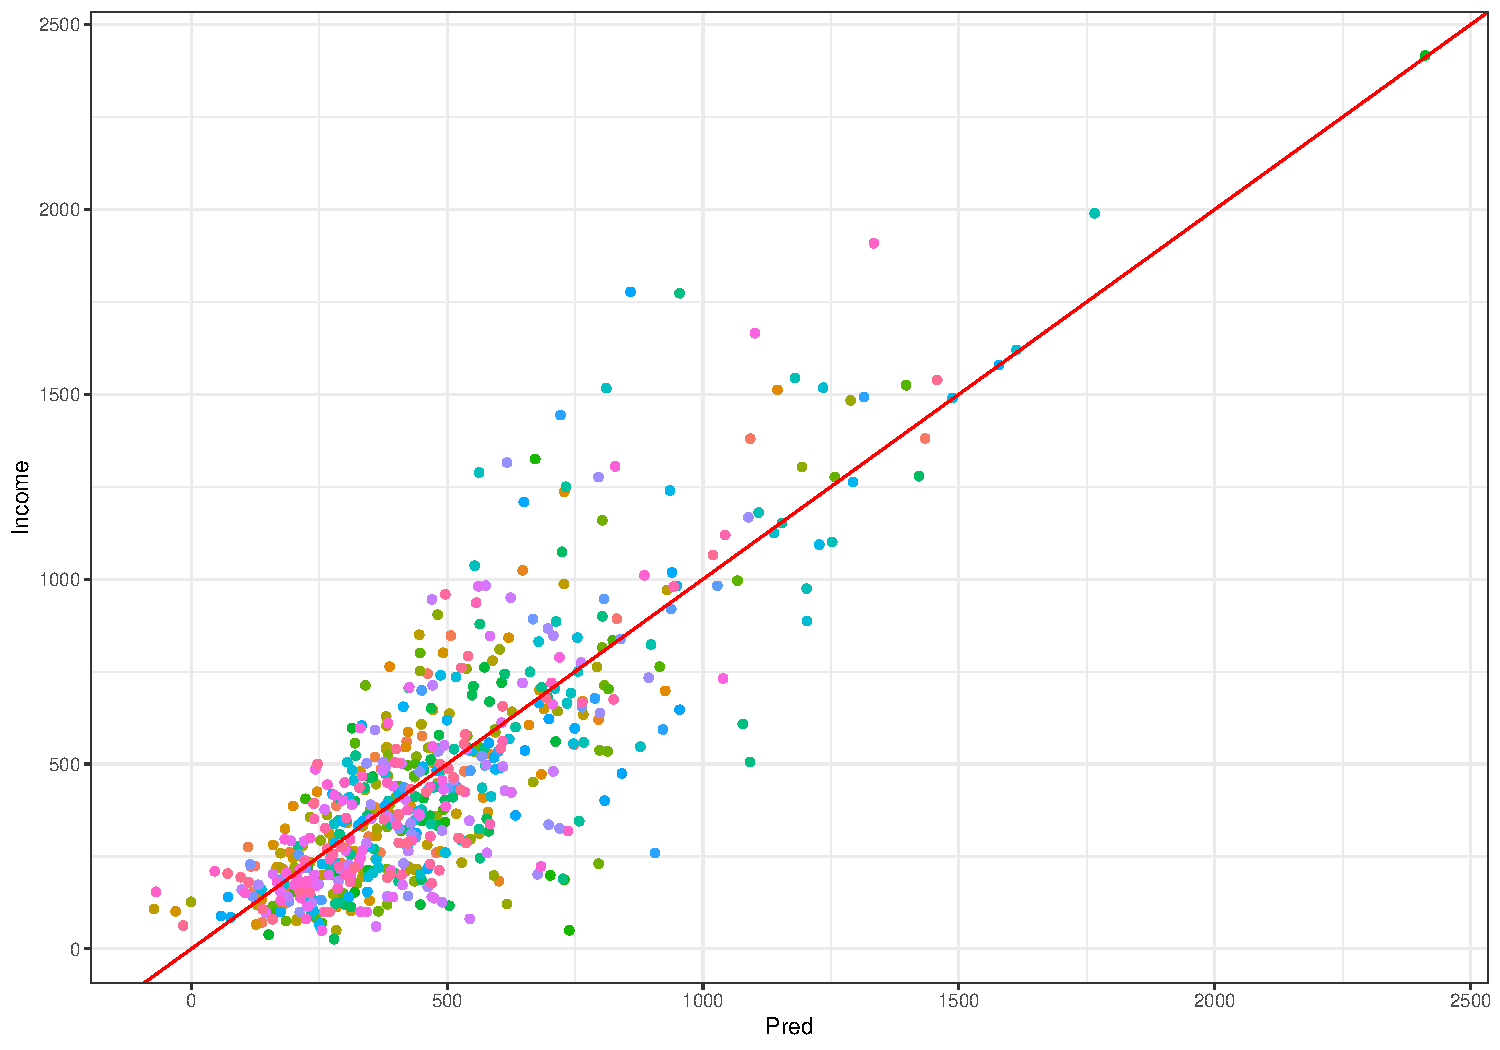
\includegraphics{07-Gráficas_files/figure-latex/unnamed-chunk-23-1.pdf}

Definiendo el color del relleno para hombres y mujeres:

\begin{Shaded}
\begin{Highlighting}[]
\NormalTok{colorSex }\OtherTok{\textless{}{-}} \FunctionTok{c}\NormalTok{(}\AttributeTok{Male =} \StringTok{"\#5DADE2"}\NormalTok{, }\AttributeTok{Female =} \StringTok{"\#2874A6"}\NormalTok{)}
\NormalTok{plot11\_Ponde }\SpecialCharTok{+} \FunctionTok{scale\_fill\_manual}\NormalTok{(}\AttributeTok{values =}\NormalTok{ colorSex) }\SpecialCharTok{|}
\NormalTok{  plot12\_Ponde }\SpecialCharTok{+} \FunctionTok{scale\_fill\_manual}\NormalTok{(}\AttributeTok{values =}\NormalTok{ colorSex)}
\end{Highlighting}
\end{Shaded}

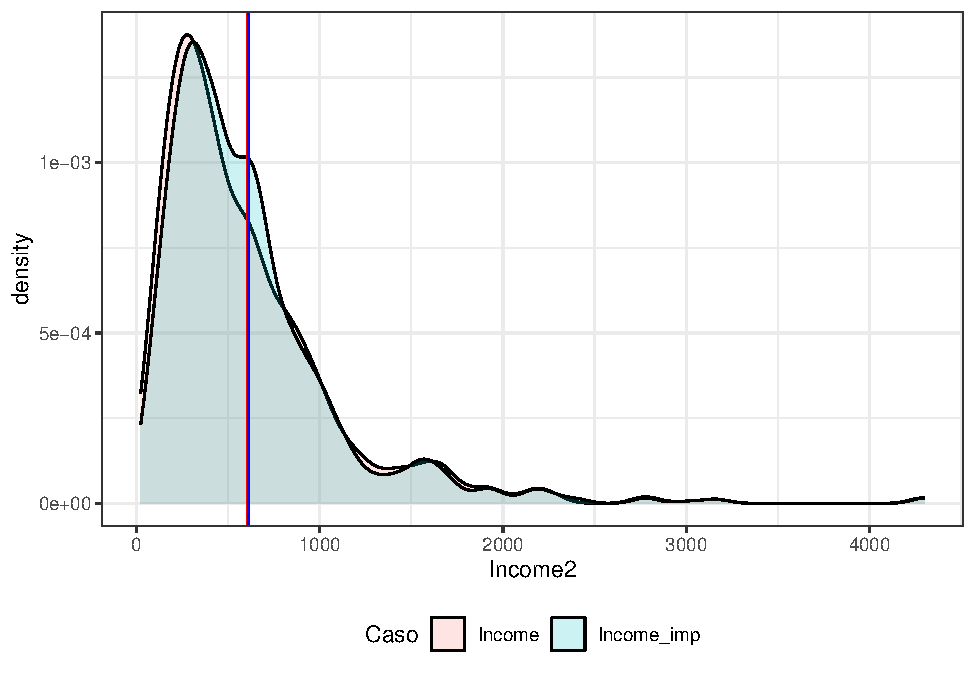
\includegraphics{07-Gráficas_files/figure-latex/unnamed-chunk-24-1.pdf}
Realizando la comparación para más de dos categorías, por ejemplo región, se procede como:

\begin{Shaded}
\begin{Highlighting}[]
\NormalTok{plot13\_Ponde }\OtherTok{\textless{}{-}} \FunctionTok{ggplot}\NormalTok{(}
  \AttributeTok{data =}\NormalTok{ encuesta,}
  \FunctionTok{aes}\NormalTok{(}\AttributeTok{x =}\NormalTok{ Income, }\AttributeTok{weight =}\NormalTok{ wk)) }\SpecialCharTok{+}
  \FunctionTok{geom\_boxplot}\NormalTok{(}\FunctionTok{aes}\NormalTok{(}\AttributeTok{fill =}\NormalTok{ Region)) }\SpecialCharTok{+}
  \FunctionTok{ggtitle}\NormalTok{(}\StringTok{"Ponderado"}\NormalTok{) }\SpecialCharTok{+}
  \FunctionTok{coord\_flip}\NormalTok{() }\SpecialCharTok{+}
  \FunctionTok{theme\_cepal}\NormalTok{()}

\NormalTok{plot14\_Ponde }\OtherTok{\textless{}{-}} \FunctionTok{ggplot}\NormalTok{(}
  \AttributeTok{data =}\NormalTok{ encuesta,}
  \FunctionTok{aes}\NormalTok{(}\AttributeTok{x =}\NormalTok{ Expenditure, }\AttributeTok{weight =}\NormalTok{ wk)) }\SpecialCharTok{+}
  \FunctionTok{geom\_boxplot}\NormalTok{(}\FunctionTok{aes}\NormalTok{(}\AttributeTok{fill =}\NormalTok{ Region)) }\SpecialCharTok{+}
  \FunctionTok{ggtitle}\NormalTok{(}\StringTok{"Ponderado"}\NormalTok{) }\SpecialCharTok{+}
  \FunctionTok{coord\_flip}\NormalTok{() }\SpecialCharTok{+}
  \FunctionTok{theme\_cepal}\NormalTok{()}

\NormalTok{plot13\_Ponde }\SpecialCharTok{|}\NormalTok{ plot14\_Ponde}
\end{Highlighting}
\end{Shaded}

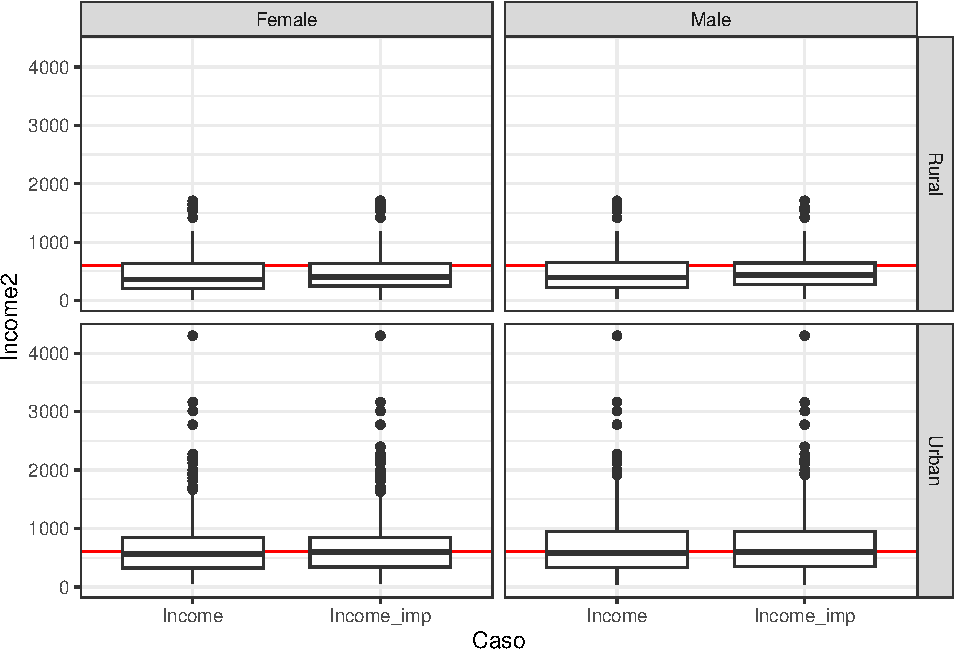
\includegraphics{07-Gráficas_files/figure-latex/unnamed-chunk-25-1.pdf}

Personalizando los coles cuando hay más de dos categorías, se realiza como se muestra a continuación:

\begin{Shaded}
\begin{Highlighting}[]
\NormalTok{colorRegion }\OtherTok{\textless{}{-}} \FunctionTok{c}\NormalTok{(}
  \AttributeTok{Norte =} \StringTok{"\#D6EAF8"}\NormalTok{, }\AttributeTok{Sur =} \StringTok{"\#85C1E9"}\NormalTok{,}
  \AttributeTok{Centro =} \StringTok{"\#3498DB"}\NormalTok{, }\AttributeTok{Occidente =} \StringTok{"\#2E86C1"}\NormalTok{, }\AttributeTok{Oriente =} \StringTok{"\#21618C"}
\NormalTok{)}
\NormalTok{plot13\_Ponde }\SpecialCharTok{+} \FunctionTok{scale\_fill\_manual}\NormalTok{(}\AttributeTok{values =}\NormalTok{ colorRegion) }\SpecialCharTok{|}
\NormalTok{plot14\_Ponde }\SpecialCharTok{+} \FunctionTok{scale\_fill\_manual}\NormalTok{(}\AttributeTok{values =}\NormalTok{ colorRegion)}
\end{Highlighting}
\end{Shaded}

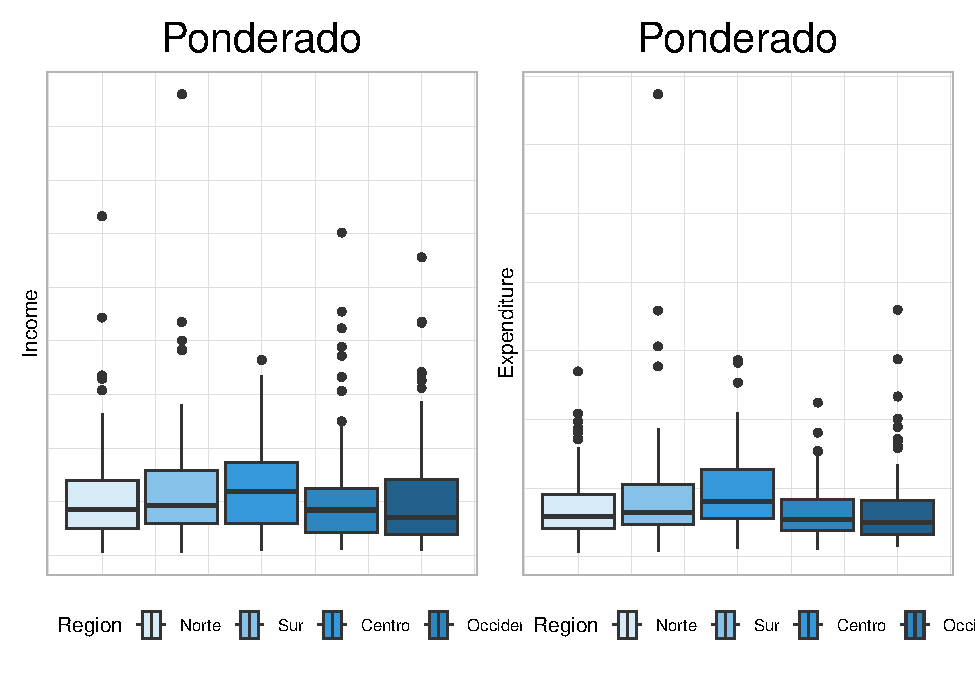
\includegraphics{07-Gráficas_files/figure-latex/unnamed-chunk-26-1.pdf}

La función \texttt{geom\_boxplot}permite realizar comparaciones con más de dos variables al tiempo. A continuación se compara los ingresos por sexo en las diferentes zonas.

\begin{Shaded}
\begin{Highlighting}[]
\NormalTok{plot15\_Ponde }\OtherTok{\textless{}{-}}\FunctionTok{ggplot}\NormalTok{(}\AttributeTok{data =}\NormalTok{ encuesta,}
    \FunctionTok{aes}\NormalTok{(}\AttributeTok{x =}\NormalTok{ Income, }\AttributeTok{y =}\NormalTok{ Zone, }\AttributeTok{weight =}\NormalTok{ wk)) }\SpecialCharTok{+}
  \FunctionTok{geom\_boxplot}\NormalTok{(}\FunctionTok{aes}\NormalTok{(}\AttributeTok{fill =}\NormalTok{ Sex)) }\SpecialCharTok{+}
  \FunctionTok{ggtitle}\NormalTok{(}\StringTok{"Ponderado"}\NormalTok{) }\SpecialCharTok{+}
  \FunctionTok{scale\_fill\_manual}\NormalTok{(}\AttributeTok{values =}\NormalTok{ colorSex) }\SpecialCharTok{+}
  \FunctionTok{coord\_flip}\NormalTok{()}
\NormalTok{plot15\_Ponde}
\end{Highlighting}
\end{Shaded}

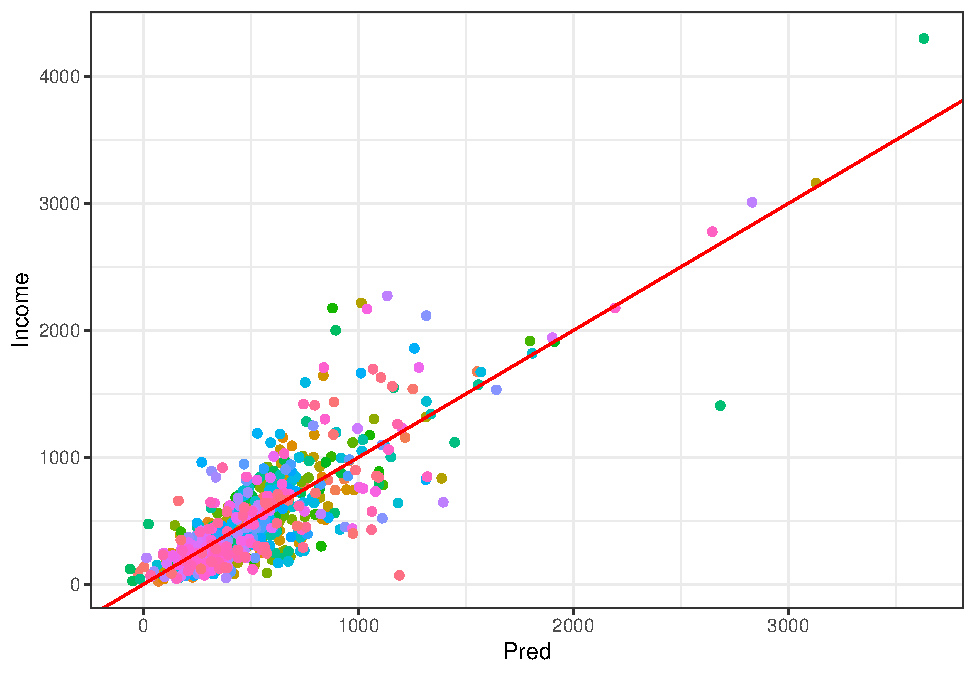
\includegraphics{07-Gráficas_files/figure-latex/unnamed-chunk-27-1.pdf}

De forma análoga podemos realizar la comparación de los gastos por sexo en las diferentes zonas:

\begin{Shaded}
\begin{Highlighting}[]
\NormalTok{plot16\_Ponde }\OtherTok{\textless{}{-}} \FunctionTok{ggplot}\NormalTok{(}\AttributeTok{data =}\NormalTok{ encuesta,}
    \FunctionTok{aes}\NormalTok{(}\AttributeTok{x =}\NormalTok{ Expenditure, }\AttributeTok{y =}\NormalTok{ Zone, }\AttributeTok{weight =}\NormalTok{ wk)) }\SpecialCharTok{+}
  \FunctionTok{geom\_boxplot}\NormalTok{(}\FunctionTok{aes}\NormalTok{(}\AttributeTok{fill =}\NormalTok{ Sex)) }\SpecialCharTok{+}
  \FunctionTok{ggtitle}\NormalTok{(}\StringTok{"Ponderado"}\NormalTok{) }\SpecialCharTok{+}
  \FunctionTok{scale\_fill\_manual}\NormalTok{(}\AttributeTok{values =}\NormalTok{ colorSex) }\SpecialCharTok{+}
  \FunctionTok{coord\_flip}\NormalTok{()}
\NormalTok{plot15\_Ponde }\SpecialCharTok{/}\NormalTok{ plot16\_Ponde}
\end{Highlighting}
\end{Shaded}

Se puede extender las comparaciones a variables que tienen más de dos categorías.

\begin{Shaded}
\begin{Highlighting}[]
\NormalTok{plot17\_Ponde }\OtherTok{\textless{}{-}} \FunctionTok{ggplot}\NormalTok{(}\AttributeTok{data =}\NormalTok{ encuesta,}
    \FunctionTok{aes}\NormalTok{(}\AttributeTok{x =}\NormalTok{ Income, }\AttributeTok{y =}\NormalTok{ Region, }\AttributeTok{weight =}\NormalTok{ wk)) }\SpecialCharTok{+}
  \FunctionTok{geom\_boxplot}\NormalTok{(}\FunctionTok{aes}\NormalTok{(}\AttributeTok{fill =}\NormalTok{ Sex)) }\SpecialCharTok{+}
  \FunctionTok{ggtitle}\NormalTok{(}\StringTok{"Ponderado"}\NormalTok{) }\SpecialCharTok{+}
  \FunctionTok{scale\_fill\_manual}\NormalTok{(}\AttributeTok{values =}\NormalTok{ colorSex) }\SpecialCharTok{+}
  \FunctionTok{coord\_flip}\NormalTok{()}
\NormalTok{plot17\_Ponde}
\end{Highlighting}
\end{Shaded}

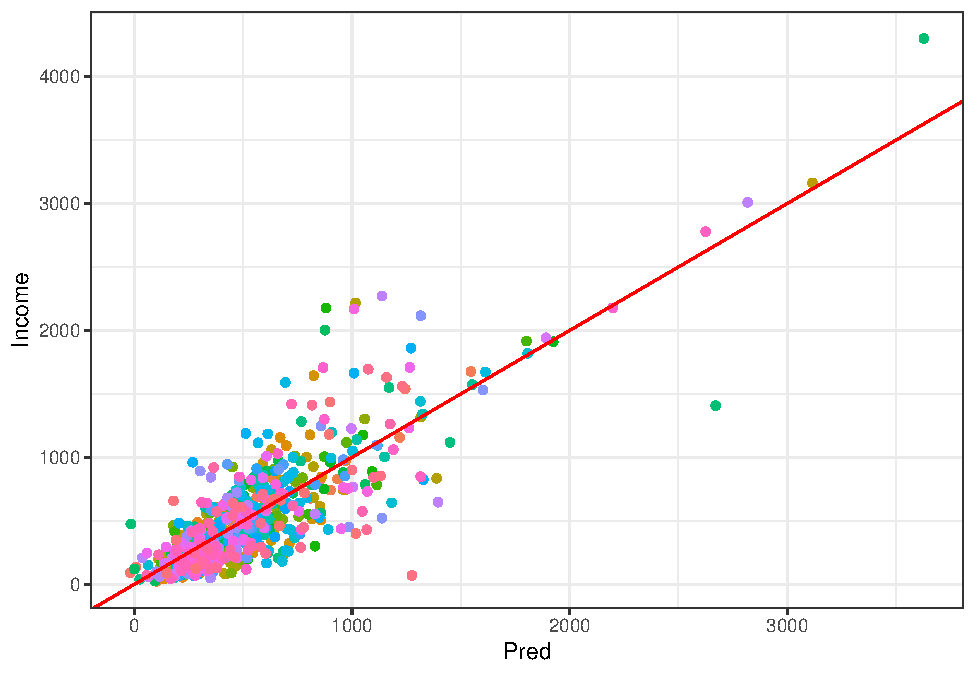
\includegraphics{07-Gráficas_files/figure-latex/unnamed-chunk-29-1.pdf}

\begin{Shaded}
\begin{Highlighting}[]
\NormalTok{plot18\_Ponde }\OtherTok{\textless{}{-}} \FunctionTok{ggplot}\NormalTok{(}\AttributeTok{data =}\NormalTok{ encuesta,}
    \FunctionTok{aes}\NormalTok{(}\AttributeTok{x =}\NormalTok{ Expenditure,}
        \AttributeTok{y =}\NormalTok{ Region, }\AttributeTok{weight =}\NormalTok{ wk)) }\SpecialCharTok{+}
  \FunctionTok{geom\_boxplot}\NormalTok{(}\FunctionTok{aes}\NormalTok{(}\AttributeTok{fill =}\NormalTok{ Sex)) }\SpecialCharTok{+}
  \FunctionTok{ggtitle}\NormalTok{(}\StringTok{"Ponderado"}\NormalTok{) }\SpecialCharTok{+}
  \FunctionTok{scale\_fill\_manual}\NormalTok{(}\AttributeTok{values =}\NormalTok{ colorSex) }\SpecialCharTok{+}
  \FunctionTok{coord\_flip}\NormalTok{()}

\NormalTok{plot17\_Ponde }\SpecialCharTok{/}\NormalTok{ plot18\_Ponde}
\end{Highlighting}
\end{Shaded}

\hypertarget{scaterplot}{%
\section{Scaterplot}\label{scaterplot}}

Un diagrama de dispersión o Scaterplot representa cada observación como un punto, posicionado según el valor de dos variables. Además de una posición horizontal y vertical, cada punto también tiene un tamaño, un color y una forma. Estos atributos se denominan estética y son las propiedades que se pueden percibir en el gráfico. Cada estética puede asignarse a una variable o establecerse en un valor constante. Para realizar este tipo de gráfico se usará la función \texttt{geom\_point}. Para ejemplificar el uso de esta función, se graficarán las variables ingresos y gastos como se muestra a continuación:

\begin{Shaded}
\begin{Highlighting}[]
\NormalTok{plot19\_Ponde }\OtherTok{\textless{}{-}} \FunctionTok{ggplot}\NormalTok{( }
  \AttributeTok{data =}\NormalTok{ encuesta,}
      \FunctionTok{aes}\NormalTok{(}
      \AttributeTok{y =}\NormalTok{ Income,}
      \AttributeTok{x =}\NormalTok{ Expenditure,}
      \AttributeTok{weight =}\NormalTok{ wk)) }\SpecialCharTok{+}
  \FunctionTok{geom\_point}\NormalTok{() }\SpecialCharTok{+}
  \FunctionTok{theme\_cepal}\NormalTok{()}
\NormalTok{plot19\_Ponde}
\end{Highlighting}
\end{Shaded}

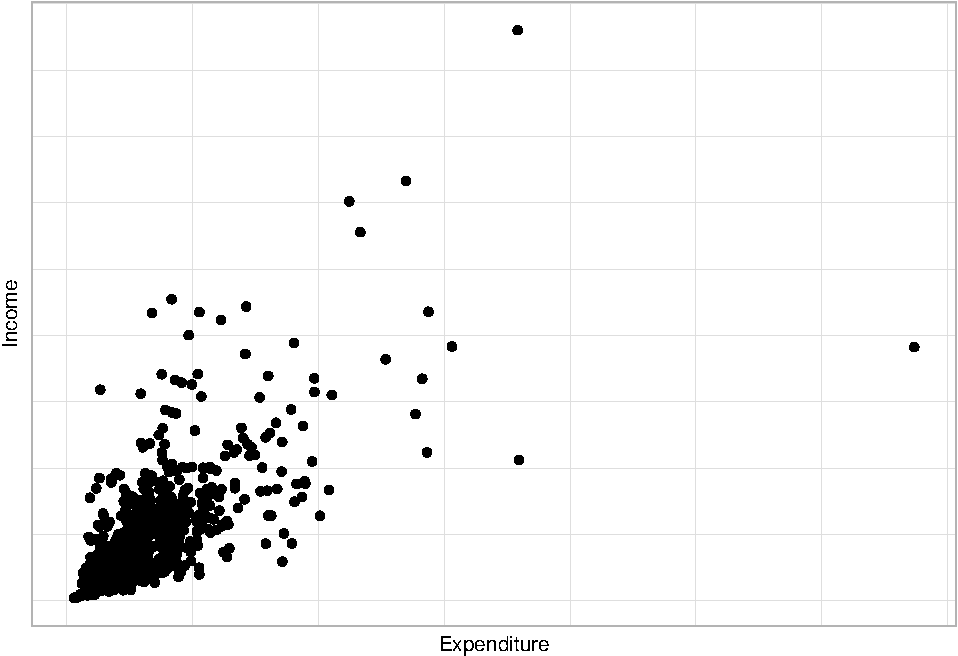
\includegraphics{07-Gráficas_files/figure-latex/unnamed-chunk-31-1.pdf}
Note, que en este caso el parámetro \texttt{weight} no está aportando información visual al gráfico. El parámetro \texttt{weight} se puede usar para controlar el tamaño de los puntos, y así, tener un mejor panorama del comportamiento de la muestra:

\begin{Shaded}
\begin{Highlighting}[]
\NormalTok{plot20\_Ponde }\OtherTok{\textless{}{-}} \FunctionTok{ggplot}\NormalTok{(}
  \AttributeTok{data =}\NormalTok{ encuesta,}
    \FunctionTok{aes}\NormalTok{(}\AttributeTok{y =}\NormalTok{ Income, }\AttributeTok{x =}\NormalTok{ Expenditure)) }\SpecialCharTok{+}
  \FunctionTok{geom\_point}\NormalTok{(}\FunctionTok{aes}\NormalTok{(}\AttributeTok{size =}\NormalTok{ wk), }\AttributeTok{alpha =} \FloatTok{0.3}\NormalTok{) }\SpecialCharTok{+}
  \FunctionTok{theme\_cepal}\NormalTok{()}
\NormalTok{plot20\_Ponde}
\end{Highlighting}
\end{Shaded}

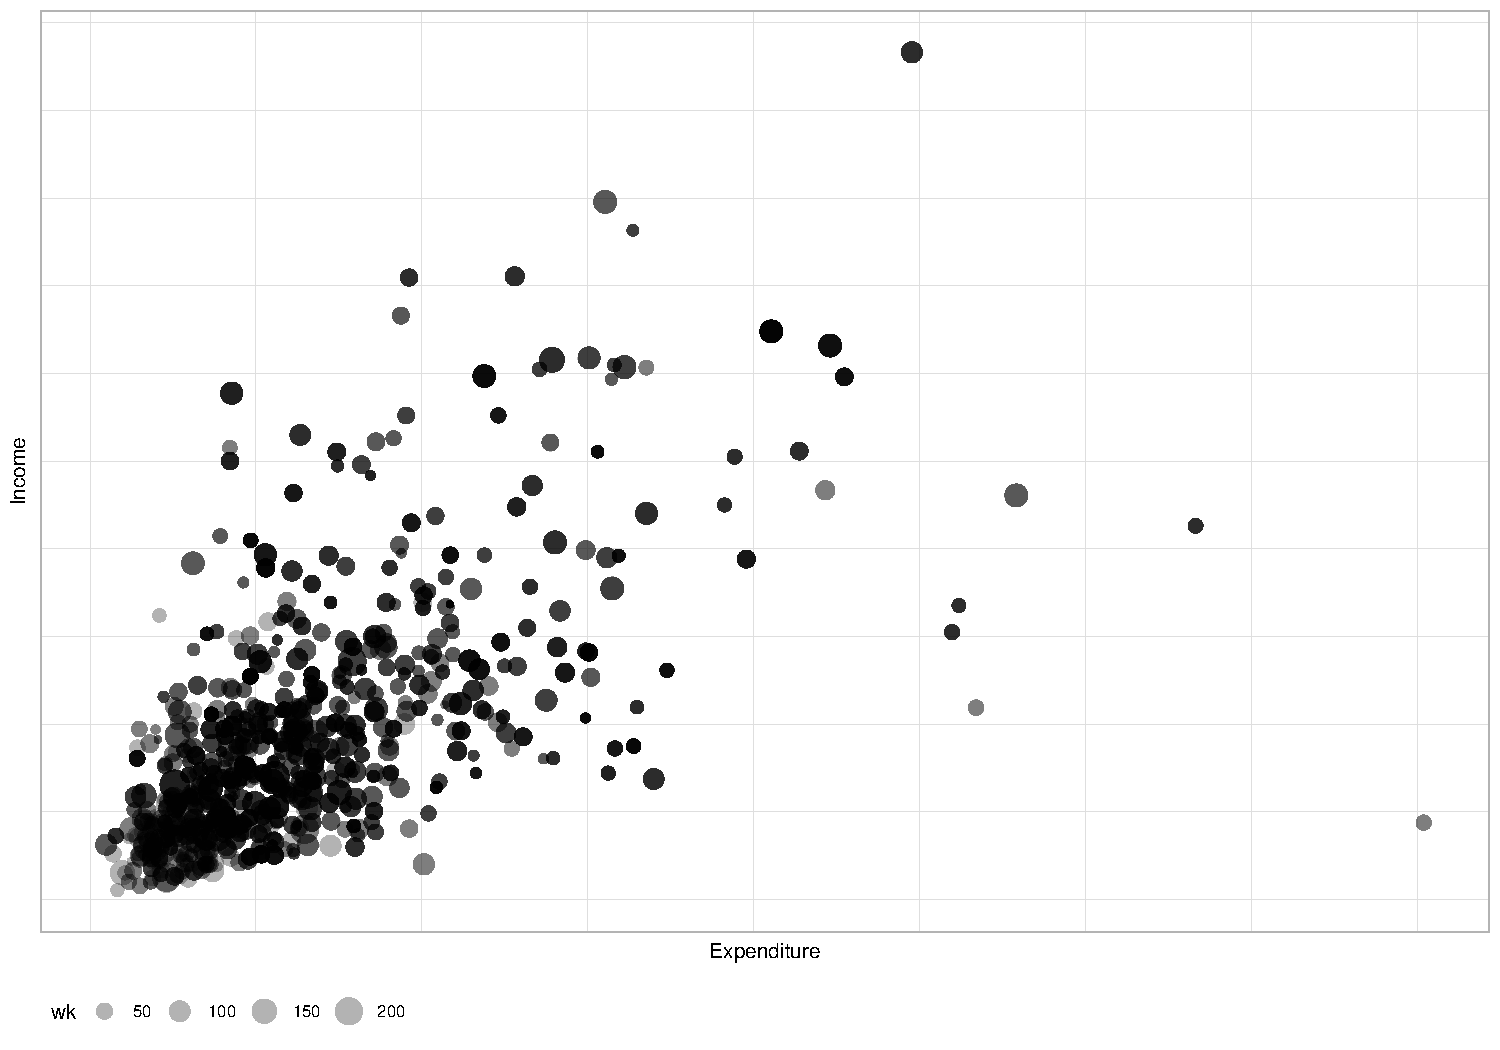
\includegraphics{07-Gráficas_files/figure-latex/hist14-1.pdf}

Otra forma de usar la variable \texttt{wk}, es asignar la intensidad del color según el valor de la variable:

\begin{Shaded}
\begin{Highlighting}[]
\NormalTok{plot21\_Ponde }\OtherTok{\textless{}{-}} \FunctionTok{ggplot}\NormalTok{(}
  \AttributeTok{data =}\NormalTok{ encuesta,}
    \FunctionTok{aes}\NormalTok{(}\AttributeTok{y =}\NormalTok{ Income, }\AttributeTok{x =}\NormalTok{ Expenditure)) }\SpecialCharTok{+}
  \FunctionTok{geom\_point}\NormalTok{(}\FunctionTok{aes}\NormalTok{(}\AttributeTok{col =}\NormalTok{ wk), }\AttributeTok{alpha =} \FloatTok{0.3}\NormalTok{) }\SpecialCharTok{+}
  \FunctionTok{theme\_cepal}\NormalTok{()}
\NormalTok{plot21\_Ponde}
\end{Highlighting}
\end{Shaded}

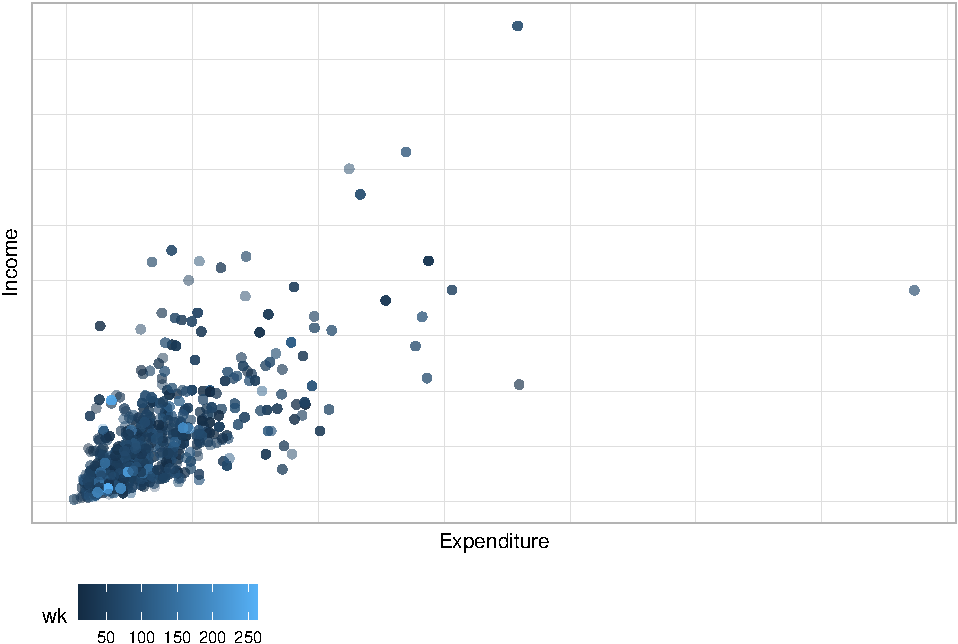
\includegraphics{07-Gráficas_files/figure-latex/unnamed-chunk-32-1.pdf}

Se puede extender las bondades de los gráfico de \texttt{ggplot2} para obtener mayor información de las muestra. Por ejemplo, agrupar los datos por Zona. Para lograr esto se introduce el parámetro \texttt{shape}:

\begin{Shaded}
\begin{Highlighting}[]
\NormalTok{plot22\_Ponde }\OtherTok{\textless{}{-}} \FunctionTok{ggplot}\NormalTok{(}
  \AttributeTok{data =}\NormalTok{ encuesta,}
    \FunctionTok{aes}\NormalTok{(}\AttributeTok{y =}\NormalTok{ Income, }
        \AttributeTok{x =}\NormalTok{ Expenditure,}
        \AttributeTok{shape =}\NormalTok{ Zone)) }\SpecialCharTok{+} 
  \FunctionTok{geom\_point}\NormalTok{(}\FunctionTok{aes}\NormalTok{(}\AttributeTok{size =}\NormalTok{ wk, }\AttributeTok{color =}\NormalTok{ Zone), }\AttributeTok{alpha =} \FloatTok{0.3}\NormalTok{) }\SpecialCharTok{+}
  \FunctionTok{labs}\NormalTok{(}\AttributeTok{size =} \StringTok{"Peso"}\NormalTok{) }\SpecialCharTok{+} \FunctionTok{scale\_color\_manual}\NormalTok{(}\AttributeTok{values =}\NormalTok{ colorZona) }\SpecialCharTok{+}
  \FunctionTok{theme\_cepal}\NormalTok{()}
\NormalTok{plot22\_Ponde}
\end{Highlighting}
\end{Shaded}

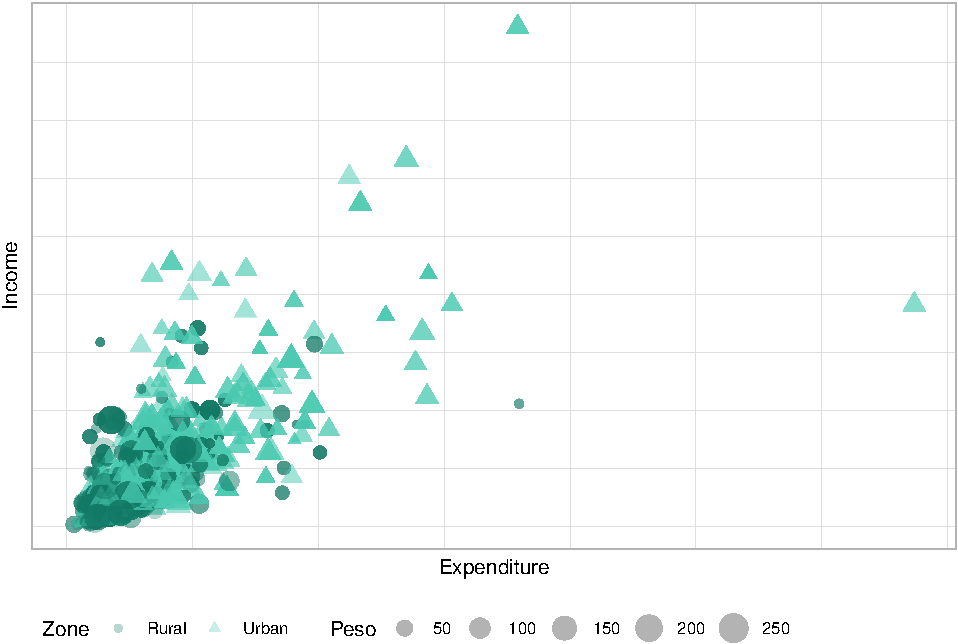
\includegraphics{07-Gráficas_files/figure-latex/unnamed-chunk-33-1.pdf}

De forma similar se puede obtener el resultado por sexo:

\begin{Shaded}
\begin{Highlighting}[]
\NormalTok{plot23\_Ponde }\OtherTok{\textless{}{-}} \FunctionTok{ggplot}\NormalTok{(}
  \AttributeTok{data =}\NormalTok{ encuesta,}
    \FunctionTok{aes}\NormalTok{(}
      \AttributeTok{y =}\NormalTok{ Income,}
      \AttributeTok{x =}\NormalTok{ Expenditure,}
      \AttributeTok{shape =}\NormalTok{ Sex)) }\SpecialCharTok{+}
  \FunctionTok{geom\_point}\NormalTok{(}\FunctionTok{aes}\NormalTok{(}
    \AttributeTok{size =}\NormalTok{ wk,}
    \AttributeTok{color =}\NormalTok{ Sex),}
  \AttributeTok{alpha =} \FloatTok{0.3}\NormalTok{) }\SpecialCharTok{+}
  \FunctionTok{labs}\NormalTok{(}\AttributeTok{size =} \StringTok{"Peso"}\NormalTok{) }\SpecialCharTok{+}
  \FunctionTok{scale\_color\_manual}\NormalTok{(}\AttributeTok{values =}\NormalTok{ colorSex) }\SpecialCharTok{+}
  \FunctionTok{theme\_cepal}\NormalTok{()}
\NormalTok{plot23\_Ponde}
\end{Highlighting}
\end{Shaded}

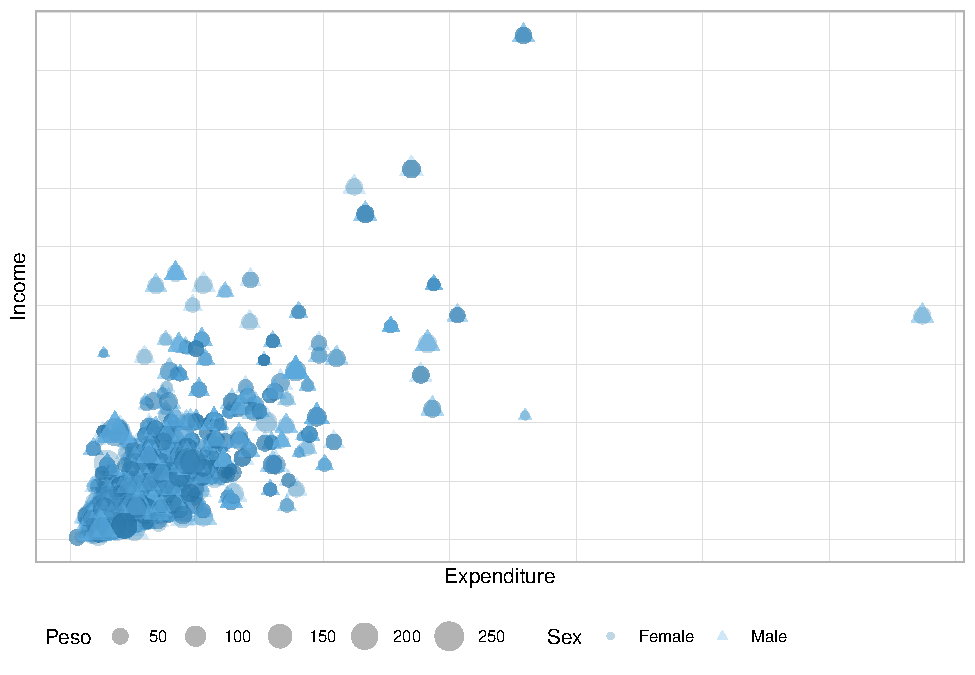
\includegraphics{07-Gráficas_files/figure-latex/unnamed-chunk-34-1.pdf}

Un resultado equivalente se obtiene por región:

\begin{Shaded}
\begin{Highlighting}[]
\NormalTok{plot24\_Ponde }\OtherTok{\textless{}{-}} \FunctionTok{ggplot}\NormalTok{(}
  \AttributeTok{data =}\NormalTok{ encuesta,}
        \FunctionTok{aes}\NormalTok{(}
      \AttributeTok{y =}\NormalTok{ Income,}
      \AttributeTok{x =}\NormalTok{ Expenditure,}
      \AttributeTok{shape =}\NormalTok{ Region)) }\SpecialCharTok{+}
  \FunctionTok{geom\_point}\NormalTok{(}\FunctionTok{aes}\NormalTok{(}
    \AttributeTok{size =}\NormalTok{ wk,}
    \AttributeTok{color =}\NormalTok{ Region),}
  \AttributeTok{alpha =} \FloatTok{0.3}\NormalTok{) }\SpecialCharTok{+}
  \FunctionTok{labs}\NormalTok{(}\AttributeTok{size =} \StringTok{"Peso"}\NormalTok{) }\SpecialCharTok{+}
  \FunctionTok{scale\_color\_manual}\NormalTok{(}\AttributeTok{values =}\NormalTok{ colorRegion) }\SpecialCharTok{+}
  \FunctionTok{theme\_cepal}\NormalTok{()}
\NormalTok{plot24\_Ponde}
\end{Highlighting}
\end{Shaded}

\includegraphics{07-Gráficas_files/figure-latex/unnamed-chunk-35-1.pdf}

\hypertarget{diagrama-de-barras-para-variables-categoricas}{%
\section{Diagrama de barras para variables categoricas}\label{diagrama-de-barras-para-variables-categoricas}}

Para realizar estos gráfico, en primer lugar, se deben realizar las estimaciones puntuales de los tamaños que se van a graficar:

\begin{Shaded}
\begin{Highlighting}[]
\NormalTok{tamano\_zona }\OtherTok{\textless{}{-}}\NormalTok{ diseno }\SpecialCharTok{\%\textgreater{}\%}
  \FunctionTok{group\_by}\NormalTok{(Zone) }\SpecialCharTok{\%\textgreater{}\%}
  \FunctionTok{summarise}\NormalTok{( }\AttributeTok{Nd =} \FunctionTok{survey\_total}\NormalTok{(}\AttributeTok{vartype =} \FunctionTok{c}\NormalTok{(}\StringTok{"se"}\NormalTok{, }\StringTok{"ci"}\NormalTok{)))}
\NormalTok{tamano\_zona }
\end{Highlighting}
\end{Shaded}

\begin{tabular}{l|r|r|r|r}
\hline
Zone & Nd & Nd\_se & Nd\_low & Nd\_upp\\
\hline
Rural & 72102 & 3062 & 66039 & 78165\\
\hline
Urban & 78164 & 2847 & 72526 & 83802\\
\hline
\end{tabular}

Ahora, se procede a hacer el gráfico como se mostró en las secciones anteriores:

\begin{Shaded}
\begin{Highlighting}[]
\NormalTok{plot25\_Ponde }\OtherTok{\textless{}{-}} \FunctionTok{ggplot}\NormalTok{(}
  \AttributeTok{data =}\NormalTok{ tamano\_zona, }
  \FunctionTok{aes}\NormalTok{(}
    \AttributeTok{x =}\NormalTok{ Zone,         }
    \AttributeTok{y =}\NormalTok{ Nd,           }
    \AttributeTok{ymax =}\NormalTok{ Nd\_upp,    }
    \AttributeTok{ymin =}\NormalTok{ Nd\_low,    }
    \AttributeTok{fill =}\NormalTok{ Zone)) }\SpecialCharTok{+}
  \FunctionTok{geom\_bar}\NormalTok{(}\AttributeTok{stat =} \StringTok{"identity"}\NormalTok{, }\AttributeTok{position =} \StringTok{"dodge"}\NormalTok{) }\SpecialCharTok{+}
  \FunctionTok{geom\_errorbar}\NormalTok{(}\AttributeTok{position =} \FunctionTok{position\_dodge}\NormalTok{(}\AttributeTok{width =} \FloatTok{0.9}\NormalTok{),}
    \AttributeTok{width =} \FloatTok{0.3}\NormalTok{) }\SpecialCharTok{+}
  \FunctionTok{theme\_bw}\NormalTok{()}
\NormalTok{plot25\_Ponde}
\end{Highlighting}
\end{Shaded}

\includegraphics{07-Gráficas_files/figure-latex/unnamed-chunk-37-1.pdf}

Como se ha visto en los gráficos anteriores, se pueden extender a variables con muchas más categorías:

\begin{Shaded}
\begin{Highlighting}[]
\NormalTok{tamano\_pobreza }\OtherTok{\textless{}{-}}\NormalTok{ diseno }\SpecialCharTok{\%\textgreater{}\%}
  \FunctionTok{group\_by}\NormalTok{(Poverty) }\SpecialCharTok{\%\textgreater{}\%}
  \FunctionTok{summarise}\NormalTok{(}\AttributeTok{Nd =} \FunctionTok{survey\_total}\NormalTok{(}\AttributeTok{vartype =} \FunctionTok{c}\NormalTok{(}\StringTok{"se"}\NormalTok{, }\StringTok{"ci"}\NormalTok{)))}
\NormalTok{tamano\_pobreza}
\end{Highlighting}
\end{Shaded}

\begin{tabular}{l|r|r|r|r}
\hline
Poverty & Nd & Nd\_se & Nd\_low & Nd\_upp\\
\hline
NotPoor & 91398 & 4395 & 82696 & 100101\\
\hline
Extreme & 21519 & 4949 & 11719 & 31319\\
\hline
Relative & 37349 & 3695 & 30032 & 44666\\
\hline
\end{tabular}

El gráfico se obtiene con una sintaxis homologa a la anterior:

\begin{Shaded}
\begin{Highlighting}[]
\NormalTok{plot26\_Ponde }\OtherTok{\textless{}{-}} \FunctionTok{ggplot}\NormalTok{(}
  \AttributeTok{data =}\NormalTok{ tamano\_pobreza,}
  \FunctionTok{aes}\NormalTok{(}
    \AttributeTok{x =}\NormalTok{ Poverty,}
    \AttributeTok{y =}\NormalTok{ Nd,}
    \AttributeTok{ymax =}\NormalTok{ Nd\_upp,}
    \AttributeTok{ymin =}\NormalTok{ Nd\_low,}
    \AttributeTok{fill =}\NormalTok{ Poverty)) }\SpecialCharTok{+}
  \FunctionTok{geom\_bar}\NormalTok{(}\AttributeTok{stat =} \StringTok{"identity"}\NormalTok{, }\AttributeTok{position =} \StringTok{"dodge"}\NormalTok{) }\SpecialCharTok{+}
  \FunctionTok{geom\_errorbar}\NormalTok{(}
    \AttributeTok{position =} \FunctionTok{position\_dodge}\NormalTok{(}\AttributeTok{width =} \FloatTok{0.9}\NormalTok{),}
    \AttributeTok{width =} \FloatTok{0.3}\NormalTok{) }\SpecialCharTok{+}
  \FunctionTok{theme\_bw}\NormalTok{()}
\NormalTok{plot26\_Ponde}
\end{Highlighting}
\end{Shaded}

\includegraphics{07-Gráficas_files/figure-latex/unnamed-chunk-39-1.pdf}

De forma similar a los gráficos Boxplot, es posible realizar comparaciones entre más dos variables.

\begin{Shaded}
\begin{Highlighting}[]
\NormalTok{tamano\_ocupacion\_pobreza }\OtherTok{\textless{}{-}}\NormalTok{ diseno }\SpecialCharTok{\%\textgreater{}\%}
  \FunctionTok{group\_by}\NormalTok{(desempleo, Poverty) }\SpecialCharTok{\%\textgreater{}\%}
  \FunctionTok{summarise}\NormalTok{(}\AttributeTok{Nd =} \FunctionTok{survey\_total}\NormalTok{(}\AttributeTok{vartype =} \FunctionTok{c}\NormalTok{(}\StringTok{"se"}\NormalTok{, }\StringTok{"ci"}\NormalTok{))) }\SpecialCharTok{\%\textgreater{}\%} \FunctionTok{as.data.frame}\NormalTok{() }\SpecialCharTok{\%\textgreater{}\%} 
  \FunctionTok{mutate}\NormalTok{(}\AttributeTok{desempleo =} \FunctionTok{ifelse}\NormalTok{(}\FunctionTok{is.na}\NormalTok{(desempleo),}\StringTok{"Ninos"}\NormalTok{,desempleo))}
\NormalTok{tamano\_ocupacion\_pobreza}
\end{Highlighting}
\end{Shaded}

\begin{tabular}{l|l|r|r|r|r}
\hline
desempleo & Poverty & Nd & Nd\_se & Nd\_low & Nd\_upp\\
\hline
0 & NotPoor & 68946 & 3676.3 & 61666.8 & 76226\\
\hline
0 & Extreme & 11549 & 2208.8 & 7175.8 & 15923\\
\hline
0 & Relative & 22847 & 2558.5 & 17780.5 & 27913\\
\hline
1 & NotPoor & 1768 & 405.4 & 965.7 & 2571\\
\hline
1 & Extreme & 1169 & 348.1 & 479.9 & 1859\\
\hline
1 & Relative & 1697 & 457.8 & 790.7 & 2604\\
\hline
Ninos & NotPoor & 20684 & 1256.6 & 18195.4 & 23172\\
\hline
Ninos & Extreme & 8800 & 2979.9 & 2899.7 & 14701\\
\hline
Ninos & Relative & 12805 & 1551.0 & 9733.9 & 15876\\
\hline
\end{tabular}

El gráfico para la tabla anterior queda de la siguiente manera:

\begin{Shaded}
\begin{Highlighting}[]
\NormalTok{plot27\_Ponde }\OtherTok{\textless{}{-}} \FunctionTok{ggplot}\NormalTok{(}
  \AttributeTok{data =}\NormalTok{ tamano\_ocupacion\_pobreza,}
    \FunctionTok{aes}\NormalTok{(}
      \AttributeTok{x =}\NormalTok{ Poverty,}
      \AttributeTok{y =}\NormalTok{ Nd,}
      \AttributeTok{ymax =}\NormalTok{ Nd\_upp,}
      \AttributeTok{ymin =}\NormalTok{ Nd\_low,}
      \AttributeTok{fill =} \FunctionTok{as.factor}\NormalTok{(desempleo))) }\SpecialCharTok{+}
  \FunctionTok{geom\_bar}\NormalTok{(}\AttributeTok{stat =} \StringTok{"identity"}\NormalTok{, }\AttributeTok{position =} \StringTok{"dodge"}\NormalTok{) }\SpecialCharTok{+}
  \FunctionTok{geom\_errorbar}\NormalTok{(}
    \AttributeTok{position =} \FunctionTok{position\_dodge}\NormalTok{(}\AttributeTok{width =} \FloatTok{0.9}\NormalTok{),}
    \AttributeTok{width =} \FloatTok{0.3}\NormalTok{) }\SpecialCharTok{+}
  \FunctionTok{theme\_bw}\NormalTok{()}
\NormalTok{plot27\_Ponde}
\end{Highlighting}
\end{Shaded}

\includegraphics{07-Gráficas_files/figure-latex/unnamed-chunk-41-1.pdf}

En estos gráficos también se pueden presentar proporciones, como se muestra a continuación:

\begin{Shaded}
\begin{Highlighting}[]
\NormalTok{prop\_ZonaH\_Pobreza }\OtherTok{\textless{}{-}}\NormalTok{ sub\_Hombre }\SpecialCharTok{\%\textgreater{}\%}
  \FunctionTok{group\_by}\NormalTok{(Zone, Poverty) }\SpecialCharTok{\%\textgreater{}\%}
  \FunctionTok{summarise}\NormalTok{(}\AttributeTok{prop =} \FunctionTok{survey\_prop}\NormalTok{(}\AttributeTok{vartype =} \FunctionTok{c}\NormalTok{(}\StringTok{"se"}\NormalTok{, }\StringTok{"ci"}\NormalTok{)))}
\NormalTok{prop\_ZonaH\_Pobreza}
\end{Highlighting}
\end{Shaded}

\begin{verbatim}
## # A tibble: 6 x 6
## # Groups:   Zone [2]
##   Zone  Poverty   prop prop_se prop_low prop_upp
##   <chr> <fct>    <dbl>   <dbl>    <dbl>    <dbl>
## 1 Rural NotPoor  0.549  0.0626   0.424     0.668
## 2 Rural Extreme  0.198  0.0675   0.0958    0.364
## 3 Rural Relative 0.254  0.0372   0.187     0.334
## 4 Urban NotPoor  0.660  0.0366   0.584     0.728
## 5 Urban Extreme  0.113  0.0245   0.0726    0.171
## 6 Urban Relative 0.227  0.0260   0.180     0.283
\end{verbatim}

Después de tener la tabla con los valores a presentar en el gráfico, los códigos computacionales para realizar el gráfico es el siguiente:

\begin{Shaded}
\begin{Highlighting}[]
\NormalTok{plot28\_Ponde }\OtherTok{\textless{}{-}} \FunctionTok{ggplot}\NormalTok{(}
  \AttributeTok{data =}\NormalTok{ prop\_ZonaH\_Pobreza,}
  \FunctionTok{aes}\NormalTok{(}
    \AttributeTok{x =}\NormalTok{ Poverty, }\AttributeTok{y =}\NormalTok{ prop,}
    \AttributeTok{ymax =}\NormalTok{ prop\_upp, }\AttributeTok{ymin =}\NormalTok{ prop\_low,}
    \AttributeTok{fill =}\NormalTok{ Zone)) }\SpecialCharTok{+} 
  \FunctionTok{geom\_bar}\NormalTok{(}\AttributeTok{stat =} \StringTok{"identity"}\NormalTok{, }\AttributeTok{position =} \StringTok{"dodge"}\NormalTok{) }\SpecialCharTok{+}
  \FunctionTok{geom\_errorbar}\NormalTok{(}
    \AttributeTok{position =} \FunctionTok{position\_dodge}\NormalTok{(}\AttributeTok{width =} \FloatTok{0.9}\NormalTok{),}
    \AttributeTok{width =} \FloatTok{0.3}
\NormalTok{  ) }\SpecialCharTok{+} \FunctionTok{scale\_fill\_manual}\NormalTok{(}\AttributeTok{values =}\NormalTok{ colorZona) }\SpecialCharTok{+}
  \FunctionTok{theme\_bw}\NormalTok{()}
\NormalTok{plot28\_Ponde}
\end{Highlighting}
\end{Shaded}

\includegraphics{07-Gráficas_files/figure-latex/unnamed-chunk-43-1.pdf}

Ahora bien, grafiquemos la proporción de hombres en condición de pobreza por región:

\begin{Shaded}
\begin{Highlighting}[]
\NormalTok{prop\_RegionH\_Pobreza }\OtherTok{\textless{}{-}}\NormalTok{ sub\_Hombre }\SpecialCharTok{\%\textgreater{}\%}
  \FunctionTok{group\_by}\NormalTok{(Region, pobreza) }\SpecialCharTok{\%\textgreater{}\%}
  \FunctionTok{summarise}\NormalTok{(}
    \AttributeTok{prop =} \FunctionTok{survey\_prop}\NormalTok{(}\AttributeTok{vartype =} \FunctionTok{c}\NormalTok{(}\StringTok{"se"}\NormalTok{, }\StringTok{"ci"}\NormalTok{))) }\SpecialCharTok{\%\textgreater{}\%}
  \FunctionTok{data.frame}\NormalTok{()}
\NormalTok{prop\_RegionH\_Pobreza}
\end{Highlighting}
\end{Shaded}

\begin{tabular}{l|r|r|r|r|r}
\hline
Region & pobreza & prop & prop\_se & prop\_low & prop\_upp\\
\hline
Norte & 0 & 0.6315 & 0.0552 & 0.5171 & 0.7327\\
\hline
Norte & 1 & 0.3685 & 0.0552 & 0.2673 & 0.4829\\
\hline
Sur & 0 & 0.6134 & 0.0567 & 0.4970 & 0.7181\\
\hline
Sur & 1 & 0.3866 & 0.0567 & 0.2819 & 0.5030\\
\hline
Centro & 0 & 0.6453 & 0.0846 & 0.4666 & 0.7910\\
\hline
Centro & 1 & 0.3547 & 0.0846 & 0.2090 & 0.5334\\
\hline
Occidente & 0 & 0.6259 & 0.0439 & 0.5358 & 0.7080\\
\hline
Occidente & 1 & 0.3741 & 0.0439 & 0.2920 & 0.4642\\
\hline
Oriente & 0 & 0.5450 & 0.1012 & 0.3480 & 0.7289\\
\hline
Oriente & 1 & 0.4550 & 0.1012 & 0.2711 & 0.6520\\
\hline
\end{tabular}

El gráfico de barras es el siguiente:

\begin{Shaded}
\begin{Highlighting}[]
\NormalTok{plot29\_Ponde }\OtherTok{\textless{}{-}} \FunctionTok{ggplot}\NormalTok{(}
  \AttributeTok{data =}\NormalTok{ prop\_RegionH\_Pobreza,}
  \FunctionTok{aes}\NormalTok{(}
    \AttributeTok{x =}\NormalTok{ Region, }\AttributeTok{y =}\NormalTok{ prop,}
    \AttributeTok{ymax =}\NormalTok{ prop\_upp, }\AttributeTok{ymin =}\NormalTok{ prop\_low,}
    \AttributeTok{fill =} \FunctionTok{as.factor}\NormalTok{(pobreza))) }\SpecialCharTok{+}
  \FunctionTok{geom\_bar}\NormalTok{(}\AttributeTok{stat =} \StringTok{"identity"}\NormalTok{, }\AttributeTok{position =} \StringTok{"dodge"}\NormalTok{) }\SpecialCharTok{+}
  \FunctionTok{geom\_errorbar}\NormalTok{(}
    \AttributeTok{position =} \FunctionTok{position\_dodge}\NormalTok{(}\AttributeTok{width =} \FloatTok{0.9}\NormalTok{),}
    \AttributeTok{width =} \FloatTok{0.3}
\NormalTok{  ) }\SpecialCharTok{+}
  \FunctionTok{theme\_bw}\NormalTok{()}
\NormalTok{plot29\_Ponde}
\end{Highlighting}
\end{Shaded}

\includegraphics{07-Gráficas_files/figure-latex/unnamed-chunk-45-1.pdf}

\hypertarget{creando-mapas}{%
\section{Creando mapas}\label{creando-mapas}}

Los mapas son una herramienta gráfica poderosa para la visualización de datos. Particularmente, para indicadores sociales-demográficos estos son una gran referencia visual para desagregaciones a nivel País, región, departamento, provincia, distrito, municipio, comuna, etc. \texttt{R} posee un sin fin de métodos de programación para representar dichos mapas.

Para graficar mapas es necesario contar con información geoespacial, datos que contienen las coordenadas o delimitaciones geográficas de determinado país o región. Sitios web como \url{http://www.diva-gis.org/gdata} ofrecen de manera gratuita bases de datos o \texttt{shapes} que contienen los vectores asociados a las geografías correspondientes.

Dichos conjuntos de datos poseen observaciones sobre la longitud y latitud lo cuál permite graficar en \texttt{R} un conjunto de puntos cuya unión en el gráfico formarán las formas los polígonos que dan forma a las áreas geográficas. Entre las distintas librería para realizar mapas en \texttt{R} están \texttt{tmap} y \texttt{ggplot2}. A continuación, se ilustra cómo se generan mapas, inicalmente con la librería \texttt{tmap}:

Inicialmente, para realizar el mapa hay que contar con el archivo de \emph{shepefile} el cual se carga de la siguiente manera::

\begin{Shaded}
\begin{Highlighting}[]
\FunctionTok{library}\NormalTok{(sf)}
\FunctionTok{library}\NormalTok{(tmap)}
\NormalTok{shapeBigCity }\OtherTok{\textless{}{-}} \FunctionTok{read\_sf}\NormalTok{(}\StringTok{"Data/shapeBigCity/BigCity.shp"}\NormalTok{)}
\end{Highlighting}
\end{Shaded}

Una vez cargado el shape, el mapa se genera usando las funciones tm\_shape y lo que se desea graficar en el mapa se incluye con la función tm\_polygons. Para este ejemplo, solo grafiquemos las regiones en el mapa:

\begin{Shaded}
\begin{Highlighting}[]
\FunctionTok{tm\_shape}\NormalTok{(shapeBigCity) }\SpecialCharTok{+} 
  \FunctionTok{tm\_polygons}\NormalTok{(}\AttributeTok{col =} \StringTok{"Region"}\NormalTok{) }
\end{Highlighting}
\end{Shaded}

\includegraphics{07-Gráficas_files/figure-latex/unnamed-chunk-47-1.pdf}
Si ahora el objetivo es graficar en las regiones el procentaje de probreza para hombres, inicialmente se debe agregar esa información a la base de datos con la que se graficará el mapa como sigue:

\begin{Shaded}
\begin{Highlighting}[]
\NormalTok{shape\_temp }\OtherTok{\textless{}{-}} \FunctionTok{tm\_shape}\NormalTok{(}
\NormalTok{  shapeBigCity }\SpecialCharTok{\%\textgreater{}\%}      \CommentTok{\# shapefile}
    \FunctionTok{left\_join}\NormalTok{(          }\CommentTok{\# Agregando una variable}
\NormalTok{      prop\_RegionH\_Pobreza }\SpecialCharTok{\%\textgreater{}\%}
        \FunctionTok{filter}\NormalTok{(pobreza }\SpecialCharTok{==} \DecValTok{1}\NormalTok{), }\CommentTok{\# Filtrando el nivel de interés. }
      \AttributeTok{by =} \StringTok{"Region"}\NormalTok{))}
\end{Highlighting}
\end{Shaded}

Una vez generado la base de datos, se procede a crear el mapa. En este ejemplo, agregarán unos puntos de corte en el mapas que son definidos en el argumento brks como se muestra a continuación:

\begin{Shaded}
\begin{Highlighting}[]
\NormalTok{brks }\OtherTok{\textless{}{-}} \FunctionTok{c}\NormalTok{(}\DecValTok{0}\NormalTok{, .}\DecValTok{2}\NormalTok{, .}\DecValTok{4}\NormalTok{, .}\DecValTok{6}\NormalTok{, }\FloatTok{0.8}\NormalTok{, }\DecValTok{1}\NormalTok{)}
\NormalTok{shape\_temp }\SpecialCharTok{+} \FunctionTok{tm\_polygons}\NormalTok{(}
  \AttributeTok{col =} \StringTok{"prop"}\NormalTok{,              }
  \AttributeTok{breaks =}\NormalTok{ brks,        }
  \AttributeTok{title =} \StringTok{"pobreza"}\NormalTok{,   }
  \AttributeTok{palette =} \StringTok{"YlOrRd"}\NormalTok{) }
\end{Highlighting}
\end{Shaded}

\includegraphics{07-Gráficas_files/figure-latex/unnamed-chunk-48-1.pdf}

A modo de otro ejemplo, se desea graficar ahora los coeficientes de variación de las estimaciones de los ingresos medios obtenidas por el diseño a nivel de región:

\begin{Shaded}
\begin{Highlighting}[]
\NormalTok{prom\_region }\OtherTok{\textless{}{-}} \FunctionTok{svyby}\NormalTok{(}\SpecialCharTok{\textasciitilde{}}\NormalTok{Income, }\SpecialCharTok{\textasciitilde{}}\NormalTok{Region, diseno,}
\NormalTok{  svymean,}
  \AttributeTok{na.rm =}\NormalTok{ T, }\AttributeTok{covmat =} \ConstantTok{TRUE}\NormalTok{,}
  \AttributeTok{vartype =} \FunctionTok{c}\NormalTok{(}\StringTok{"cv"}\NormalTok{))}
\NormalTok{prom\_region}
\end{Highlighting}
\end{Shaded}

\begin{tabular}{l|l|r|r}
\hline
  & Region & Income & cv\\
\hline
Norte & Norte & 552.4 & 0.1002\\
\hline
Sur & Sur & 625.8 & 0.0997\\
\hline
Centro & Centro & 650.8 & 0.0945\\
\hline
Occidente & Occidente & 517.0 & 0.0894\\
\hline
Oriente & Oriente & 541.8 & 0.1323\\
\hline
\end{tabular}

\begin{Shaded}
\begin{Highlighting}[]
\NormalTok{brks }\OtherTok{\textless{}{-}} \FunctionTok{c}\NormalTok{(}\DecValTok{0}\NormalTok{, }\FloatTok{0.2}\NormalTok{, }\DecValTok{1}\NormalTok{)}
\NormalTok{shape\_temp }\OtherTok{\textless{}{-}} \FunctionTok{tm\_shape}\NormalTok{(}
\NormalTok{  shapeBigCity }\SpecialCharTok{\%\textgreater{}\%}
    \FunctionTok{left\_join}\NormalTok{(}
\NormalTok{      prom\_region,}
      \AttributeTok{by =} \StringTok{"Region"}\NormalTok{))}

\NormalTok{shape\_temp }\SpecialCharTok{+} \FunctionTok{tm\_polygons}\NormalTok{(}
  \StringTok{"cv"}\NormalTok{,}
  \AttributeTok{breaks =}\NormalTok{ brks,}
  \AttributeTok{title =} \StringTok{"cv"}\NormalTok{,}
  \AttributeTok{palette =} \FunctionTok{c}\NormalTok{(}\StringTok{"\#FFFFFF"}\NormalTok{, }\StringTok{"\#000000"}\NormalTok{),}
\NormalTok{) }\SpecialCharTok{+} \FunctionTok{tm\_layout}\NormalTok{(}\AttributeTok{asp =} \DecValTok{0}\NormalTok{)}
\end{Highlighting}
\end{Shaded}

\includegraphics{07-Gráficas_files/figure-latex/hist26-1.pdf}
Ahora, realizar el mismo ejercicio anterior pero por zona y sexo:

\begin{Shaded}
\begin{Highlighting}[]
\NormalTok{prom\_region\_Sex }\OtherTok{\textless{}{-}}\NormalTok{ diseno }\SpecialCharTok{\%\textgreater{}\%}
  \FunctionTok{group\_by}\NormalTok{(Region, Zone, Sex, pobreza) }\SpecialCharTok{\%\textgreater{}\%}
  \FunctionTok{summarise}\NormalTok{(}\AttributeTok{prop =} \FunctionTok{survey\_mean}\NormalTok{(}\AttributeTok{vartype =} \StringTok{"cv"}\NormalTok{)) }\SpecialCharTok{\%\textgreater{}\%}
  \FunctionTok{filter}\NormalTok{(pobreza }\SpecialCharTok{==} \DecValTok{1}\NormalTok{, Zone }\SpecialCharTok{==} \StringTok{"Rural"}\NormalTok{, Sex }\SpecialCharTok{==} \StringTok{"Female"}\NormalTok{)}

\NormalTok{shape\_temp }\OtherTok{\textless{}{-}} \FunctionTok{tm\_shape}\NormalTok{(}
\NormalTok{  shapeBigCity }\SpecialCharTok{\%\textgreater{}\%}
    \FunctionTok{left\_join}\NormalTok{(}
\NormalTok{      prom\_region\_Sex,}
      \AttributeTok{by =} \StringTok{"Region"}\NormalTok{))}

\NormalTok{shape\_temp }\SpecialCharTok{+} \FunctionTok{tm\_polygons}\NormalTok{(}
  \StringTok{"prop"}\NormalTok{,}
  \AttributeTok{title =} \StringTok{"Pobreza"}\NormalTok{,}
\NormalTok{) }\SpecialCharTok{+} \FunctionTok{tm\_layout}\NormalTok{(}\AttributeTok{asp =} \DecValTok{0}\NormalTok{)}
\end{Highlighting}
\end{Shaded}

\includegraphics{07-Gráficas_files/figure-latex/unnamed-chunk-49-1.pdf}

Como se comentó en la introducción de esta sección, los gráficos también se pueden hacer usando la librería ggplot2. Esta librería se apoya en las librerías biscale y cowplot. El procedimiento en R para hacer los mapas es muy similar al mostrado con la librería tmap y se realiza de la siguiente manera:

\begin{Shaded}
\begin{Highlighting}[]
\FunctionTok{library}\NormalTok{(biscale)}
\FunctionTok{library}\NormalTok{(cowplot)}
\NormalTok{temp\_shape }\OtherTok{\textless{}{-}}\NormalTok{ shapeBigCity }\SpecialCharTok{\%\textgreater{}\%}
  \FunctionTok{left\_join}\NormalTok{(}
\NormalTok{    prom\_region\_Sex,}
    \AttributeTok{by =} \StringTok{"Region"}\NormalTok{)}

\NormalTok{k }\OtherTok{\textless{}{-}} \DecValTok{3}
\NormalTok{datos.RM.bi }\OtherTok{\textless{}{-}} \FunctionTok{bi\_class}\NormalTok{(temp\_shape,}
  \AttributeTok{y =}\NormalTok{ prop, }\AttributeTok{x =}\NormalTok{ prop\_cv, }\AttributeTok{dim =}\NormalTok{ k,}
  \AttributeTok{style =} \StringTok{"fisher"}\NormalTok{)}

\NormalTok{map.RM }\OtherTok{\textless{}{-}} \FunctionTok{ggplot}\NormalTok{() }\SpecialCharTok{+}
  \FunctionTok{geom\_sf}\NormalTok{(}
    \AttributeTok{data =}\NormalTok{ datos.RM.bi,}
    \FunctionTok{aes}\NormalTok{(}\AttributeTok{fill =}\NormalTok{ bi\_class, }\AttributeTok{geometry =}\NormalTok{ geometry),}
    \AttributeTok{colour =} \StringTok{"white"}\NormalTok{, }\AttributeTok{size =} \FloatTok{0.1}\NormalTok{) }\SpecialCharTok{+}
  \FunctionTok{bi\_scale\_fill}\NormalTok{(}\AttributeTok{pal =} \StringTok{"GrPink"}\NormalTok{, }\AttributeTok{dim =}\NormalTok{ k) }\SpecialCharTok{+}
  \FunctionTok{bi\_theme}\NormalTok{() }\SpecialCharTok{+}
  \FunctionTok{theme}\NormalTok{(}\AttributeTok{legend.position =} \StringTok{"none"}\NormalTok{)}
\NormalTok{map.RM}
\end{Highlighting}
\end{Shaded}

\includegraphics{07-Gráficas_files/figure-latex/unnamed-chunk-50-1.pdf}

Ahora, para crear la leyenda del mapa se hace de la siguiente manera:

\begin{Shaded}
\begin{Highlighting}[]
\NormalTok{legend1 }\OtherTok{\textless{}{-}} \FunctionTok{bi\_legend}\NormalTok{(}
  \AttributeTok{pal =} \StringTok{"GrPink"}\NormalTok{, }\AttributeTok{dim =}\NormalTok{ k,}
  \AttributeTok{xlab =} \StringTok{"Coeficiente de variaci\textless{}U+00F3\textgreater{}n"}\NormalTok{,}
  \AttributeTok{ylab =} \StringTok{"Pobreza"}\NormalTok{, }\AttributeTok{size =} \DecValTok{8}\NormalTok{)}

\NormalTok{mapa1 }\OtherTok{\textless{}{-}} \FunctionTok{ggdraw}\NormalTok{() }\SpecialCharTok{+}
  \FunctionTok{draw\_plot}\NormalTok{(map.RM, }\DecValTok{0}\NormalTok{, }\DecValTok{0}\NormalTok{, }\DecValTok{1}\NormalTok{, }\AttributeTok{scale =} \FloatTok{0.7}\NormalTok{) }\SpecialCharTok{+}
  \FunctionTok{draw\_plot}\NormalTok{(legend1, }\FloatTok{0.75}\NormalTok{, }\FloatTok{0.4}\NormalTok{, }\FloatTok{0.2}\NormalTok{, }\FloatTok{0.2}\NormalTok{, }\AttributeTok{scale =} \DecValTok{1}\NormalTok{) }\SpecialCharTok{+}
  \FunctionTok{draw\_text}\NormalTok{(}\StringTok{"Estimaciones directas de la pobreza en la mujer rural"}\NormalTok{,}
    \AttributeTok{vjust =} \SpecialCharTok{{-}}\DecValTok{13}\NormalTok{, }\AttributeTok{size =} \DecValTok{18}\NormalTok{)}

\NormalTok{mapa1}
\end{Highlighting}
\end{Shaded}

\includegraphics{07-Gráficas_files/figure-latex/hist31-1.pdf}

\hypertarget{modelos-lineales-generalizados-en-encuestas-de-hogares}{%
\chapter{Modelos lineales generalizados en encuestas de hogares}\label{modelos-lineales-generalizados-en-encuestas-de-hogares}}

Los modelos lineales generalizados (MLGs) proporcionan una aproximación unificada a la mayoría de los procedimientos usados en estadística aplicada.

El nombre se debe a que ellos generalizan los modelos lineales basados en el supuesto de distribución normal para la variable respuesta. Al igual que los modelos lineales clásicos, tratados en capítulos anteriores, los MLG tienen aplicación en todas las disciplinas del saber. \emph{Nelder \& Wedderburn (1972)} presentaron por primera vez el término en un artículo que, sin lugar a dudas, es uno de los más importantes publicados en el área de estadística, por su gran impacto en la forma como se aplica esta disciplina. Desde entonces, poco a
poco los modelos lineales generalizados se han ido conociendo y usando ampliamente.

La genialidad de \emph{Nelder \& Wedderburn (1972)} consistió en darse cuenta (y demostrar) que muchos de los métodos estadísticos ampliamente usados en la época, aparentemente desligados unos de otros, tales como la regresión lineal múltiple, el análisis probit, el análisis de datos provenientes de ensayos de dilución usando la distribución binomial (realizados por Fisher), los modelos logit para proporciones, los modelos log-lineales para conteos, los modelos de regresión para datos de sobrevivencia, entre otros, se podían tratar con un marco teórico unificado y que las estimaciones de máxima verosimilitud para los parámetros de esos modelos podían obtenerse por el mismo algoritmo conocido como mínimos cuadrados ponderados iterativos (MCPI).

Los desarrollos teóricos en modelos lineales clásicos parten del supuesto que la variable respuesta tiene distribución normal, cuando un fenómeno en estudio genera datos para los cuales no es razonable la suposición de normalidad, como por ejemplo cuando la respuesta es categórica, una proporción o un conteo, obviamente la respuesta no es normal y no es recomendable analizar los datos suponiendo normalidad.

Otro supuesto de los modelos lineales clásicos es el de homogeneidad de la varianza, situación que no se verifica cuando la respuesta
es, por ejemplo, una variable aleatoria de poisson, distribución donde la media y la varianza son iguales, es decir, en este modelo un cambio en la media necesariamente implica cambio en la varianza.

Los modelos lineales generalizados son excelentes para modelar datos en condiciones de no normalidad y varianza no constante. Específicamente, se debería considerar usar los MLGs cuando la variable respuesta es: conteos expresados como proporciones, conteos que no son proporciones, respuestas binarias, tiempos de sobrevida donde la varianza se incrementa con la media.

Sin lugar a dudas, en las encuestas de hogares existen variables de tipo conteo, binomiales, etc que meritan su análisis usando modelos lineales generalizados. Es por esto que, este capítulo es de relevancia en este texto.

Para ejemplificar los conceptos, inicialmente se cargan las librerías y la base de datos como sigue:

\begin{Shaded}
\begin{Highlighting}[]
\FunctionTok{options}\NormalTok{(}\AttributeTok{digits =} \DecValTok{4}\NormalTok{)}
\FunctionTok{options}\NormalTok{(}\AttributeTok{tinytex.verbose =} \ConstantTok{TRUE}\NormalTok{)}
\FunctionTok{library}\NormalTok{ (survey)}
\FunctionTok{library}\NormalTok{(srvyr)}
\FunctionTok{library}\NormalTok{(convey)}
\FunctionTok{library}\NormalTok{(TeachingSampling)}
\FunctionTok{library}\NormalTok{(printr)}
\FunctionTok{library}\NormalTok{(stargazer)}
\FunctionTok{library}\NormalTok{(broom)}
\FunctionTok{library}\NormalTok{(jtools)}
\FunctionTok{library}\NormalTok{(modelsummary)}
\FunctionTok{library}\NormalTok{(patchwork)}
\end{Highlighting}
\end{Shaded}

Cargue de las bases de datos,

\begin{Shaded}
\begin{Highlighting}[]
\NormalTok{encuesta }\OtherTok{\textless{}{-}} \FunctionTok{readRDS}\NormalTok{(}\StringTok{"Data/encuesta.rds"}\NormalTok{)}
\FunctionTok{data}\NormalTok{(}\StringTok{"BigCity"}\NormalTok{, }\AttributeTok{package =} \StringTok{"TeachingSampling"}\NormalTok{)}
\end{Highlighting}
\end{Shaded}

Por último, se define el diseño muestral,

\begin{Shaded}
\begin{Highlighting}[]
\NormalTok{diseno }\OtherTok{\textless{}{-}}\NormalTok{ encuesta }\SpecialCharTok{\%\textgreater{}\%}
  \FunctionTok{as\_survey\_design}\NormalTok{(}
    \AttributeTok{strata =}\NormalTok{ Stratum,}
    \AttributeTok{ids =}\NormalTok{ PSU,}
    \AttributeTok{weights =}\NormalTok{ wk,}
    \AttributeTok{nest =}\NormalTok{ T}
\NormalTok{  )}
\end{Highlighting}
\end{Shaded}

Se generan nuevas variables en el diseño para ser utilizadas en los ejemplos,

\begin{Shaded}
\begin{Highlighting}[]
\NormalTok{diseno }\OtherTok{\textless{}{-}}\NormalTok{ diseno }\SpecialCharTok{\%\textgreater{}\%} \FunctionTok{mutate}\NormalTok{(}
  \AttributeTok{pobreza =} \FunctionTok{ifelse}\NormalTok{(Poverty }\SpecialCharTok{!=} \StringTok{"NotPoor"}\NormalTok{, }\DecValTok{1}\NormalTok{, }\DecValTok{0}\NormalTok{),}
  \AttributeTok{desempleo =} \FunctionTok{ifelse}\NormalTok{(Employment }\SpecialCharTok{==} \StringTok{"Unemployed"}\NormalTok{, }\DecValTok{1}\NormalTok{, }\DecValTok{0}\NormalTok{))}
\end{Highlighting}
\end{Shaded}

Como se ha definido en secciones y capítulos anteriores, con variables dicotómicas se pueden generar tablas de frecuencias teniendo en cuenta los factores de expansión del diseño. En \texttt{R} se hace usando la función \texttt{svyby} de la siguiente manera. Primero, se define la variable a la que se le requiere hacer la tabla (formula), luego se le indica cuál es la variable clasificadora (by). En este caso se quiere hacer una tabla de pobreza claificada por sexo. En tercer lugar se define la función que se quiere aplicar (FUN), en este caso, se quieren calcular totales por celda, por último, se define el diseño de muestreo (design)

\begin{Shaded}
\begin{Highlighting}[]
\NormalTok{tab\_pobreza\_sexo }\OtherTok{\textless{}{-}} \FunctionTok{svyby}\NormalTok{(}\AttributeTok{formula =} \SpecialCharTok{\textasciitilde{}}\FunctionTok{factor}\NormalTok{(pobreza), }
                          \AttributeTok{by =} \SpecialCharTok{\textasciitilde{}}\NormalTok{Sex,}
                          \AttributeTok{FUN =}\NormalTok{ svytotal, }
                          \AttributeTok{design =} \FunctionTok{as.svrepdesign}\NormalTok{(diseno), }
                          \AttributeTok{se=}\NormalTok{F, }\AttributeTok{na.rm=}\NormalTok{T, }\AttributeTok{ci=}\NormalTok{T, }\AttributeTok{keep.var=}\ConstantTok{TRUE}\NormalTok{)}
\NormalTok{tab\_pobreza\_sexo}
\end{Highlighting}
\end{Shaded}

\begin{tabular}{l|l|r|r|r|r}
\hline
  & Sex & factor(pobreza)0 & factor(pobreza)1 & se1 & se2\\
\hline
Female & Female & 48366 & 30824 & 2411 & 2916\\
\hline
Male & Male & 43032 & 28044 & 2522 & 3095\\
\hline
\end{tabular}

Sin embargo para la estimación de tamaños, se puede emplear también la función \texttt{svytable} como sigue:

\begin{Shaded}
\begin{Highlighting}[]
\NormalTok{tab }\OtherTok{\textless{}{-}} \FunctionTok{svytable}\NormalTok{(}\AttributeTok{formula =} \SpecialCharTok{\textasciitilde{}}\NormalTok{pobreza }\SpecialCharTok{+}\NormalTok{ Sex, }\AttributeTok{design =}\NormalTok{ diseno)}
\FunctionTok{kable}\NormalTok{(tab)}
\end{Highlighting}
\end{Shaded}

\begin{tabular}{l|r|r}
\hline
  & Female & Male\\
\hline
0 & 48366 & 43032\\
\hline
1 & 30824 & 28044\\
\hline
\end{tabular}

Al hacer uso de la función \texttt{svyby} pero usando en el argumento \texttt{FUN=\ svymean} es posible estimar proporciones como se muestra a continuación:

\begin{Shaded}
\begin{Highlighting}[]
\NormalTok{tab\_pobreza\_sexo }\OtherTok{\textless{}{-}} \FunctionTok{svyby}\NormalTok{(}\AttributeTok{formula =} \SpecialCharTok{\textasciitilde{}}\FunctionTok{factor}\NormalTok{(pobreza), }
                          \AttributeTok{by =} \SpecialCharTok{\textasciitilde{}}\NormalTok{Sex,}
                          \AttributeTok{FUN =}\NormalTok{ svymean, }
                          \AttributeTok{design =} \FunctionTok{as.svrepdesign}\NormalTok{(diseno), }
                          \AttributeTok{se=}\NormalTok{F, }\AttributeTok{na.rm=}\NormalTok{T, }\AttributeTok{ci=}\NormalTok{T, }\AttributeTok{keep.var=}\ConstantTok{TRUE}\NormalTok{)}
\NormalTok{tab\_pobreza\_sexo}
\end{Highlighting}
\end{Shaded}

\begin{tabular}{l|l|r|r|r|r}
\hline
  & Sex & factor(pobreza)0 & factor(pobreza)1 & se1 & se2\\
\hline
Female & Female & 0.6108 & 0.3892 & 0.0316 & 0.0316\\
\hline
Male & Male & 0.6054 & 0.3946 & 0.0366 & 0.0366\\
\hline
\end{tabular}

También se pueden hacer tablas de doble entrada para la proporción.
En forma alternativa es posible usar la función \texttt{prop.table} del paquete base.

\begin{Shaded}
\begin{Highlighting}[]
\FunctionTok{kable}\NormalTok{(}\FunctionTok{prop.table}\NormalTok{(tab, }\AttributeTok{margin =} \DecValTok{2}\NormalTok{))}
\end{Highlighting}
\end{Shaded}

\begin{tabular}{l|r|r}
\hline
  & Female & Male\\
\hline
0 & 0.6108 & 0.6054\\
\hline
1 & 0.3892 & 0.3946\\
\hline
\end{tabular}

Estas diferentes formas de proceder son de mucha importancia al momento de hacer uso de pruebas de independencia en tablas cruzadas.

\hypertarget{prueba-de-independencia-f}{%
\section{Prueba de independencia F}\label{prueba-de-independencia-f}}

La prueba de independencia F de Fisher permite analizar si dos variables dicotómicas están asociadas cuando la muestra a estudiar es demasiado pequeña y no se cumplen las condiciones para aplicar la prueba \(\chi^{2}\). Para utilizar esta técnica, tengamos en cuenta que la probabilidad estimada se escribe como:

\[
\hat{\pi}_{rc}=\frac{n_{r+}}{n_{++}}\times\frac{n_{+c}}{n_{++}}
\]
Teniendo en cuenta esta expresión, la estadística \(\chi{2}\) de Pearson se define de la siguiente manera:

\[
\chi_{pearsom}^{2}=n_{++}\times\sum_{r}\sum_{c}\left(\frac{\left(p_{rc}-\hat{\pi}_{rc}\right)^{2}}{\hat{\pi}_{rc}}\right)
\]

y la estadística de razón de verosimilitud se define como:

\[
G^{2}=2\times n_{++}\times\sum_{r}\sum_{c}p_{cr}\times\ln\left(\frac{p_{rc}}{\hat{\pi}_{rc}}\right)
\]

donde, \(r\) es el número de filas y \(c\) representa el número de columnas, la prueba tiene \((R-1)\times (C-1)\) grados de libertad.

Como lo menciona \emph{Heeringa}, \emph{Fay (1979, 1985)} y \emph{Fellegi (1980)} fueron de los primeros en proponer la corrección del estadístico chi-cuadrado de Pearson basada en un efecto de diseño generalizado (GDEFF, por sus siglas en inglés). \emph{Rao y Scott (1984)} y más tarde \emph{Thomas y Rao (1987)} ampliaron la teoría de las correcciones del efecto de diseño generalizado para estas pruebas estadísticas. El método de Rao-Scott requiere el cálculo de efectos de diseño generalizados que son analíticamente más complicados que el enfoque de Fellegi. Las correcciones de Rao-Scott son ahora el estándar en los procedimientos para el análisis de datos de encuestas categóricas en sistemas de software como Stata y SAS. Los estadísticos de prueba Rao-Scott Pearson ajustados por diseño y razón de verosimilitud chi-cuadrado se calculan de la siguiente manera:

\[
\chi^2_{(R-S)} = \chi^2_{(Pearson)}\big/GDEFF
\]
y, para la estadística basada en la razón de verosimilitud se calcula como:

\[
G^2_{(R-S)}  =  G^2\big/GDEFF
\]

donde el efecto generalizado del diseño (\(GDEFF\)) de Rao--Scott, está dado por

\[
GDEFF=\frac{\sum_{r}\sum_{c}\left(1-p_{rc}\right)d^{2}\left(p_{rc}\right)-\sum_{r}\left(1-p_{r+}\right)d^{2}\left(p_{r+}\right)-\sum_{c}\left(1-p_{+c}\right)d^{2}\left(p_{+c}\right)}{\left(R-1\right)\left(C-1\right)}
\]

Por tanto, la estadística F para independencia basada en la chi-cuadrado de Pearson se calcula como sigue:

\[
F_{R-S,Pearson}=\chi_{R-S}^{2}\big/\left[\left(R-1\right)\left(C-1\right)\right]\sim F_{\left(R-1\right)\left(C-1\right),\left(R-1\right)\left(C-1\right)df}
\]

y, la estadística F para independencia basada en la razón de verosimilitudes se calcula como sigue:

\[
F_{R-S,LRT}=G_{R-S}^{2}\big/\left(C-1\right)\sim F_{\left(C-1\right),df}
\]
donde \(C\) es el número de columnas de la tabla cruzada.

En \texttt{R}, el cálculo de las estadísticas chi-cuadrado y F se camculan usando la función \texttt{summary} como se muestra a continuación:

\begin{Shaded}
\begin{Highlighting}[]
\FunctionTok{summary}\NormalTok{(tab, }\AttributeTok{statistic =} \StringTok{"Chisq"}\NormalTok{)}
\end{Highlighting}
\end{Shaded}

\begin{verbatim}
##        Sex
## pobreza Female  Male
##       0  48366 43032
##       1  30824 28044
## 
##  Pearson's X^2: Rao & Scott adjustment
## 
## data:  NextMethod()
## X-squared = 0.077, df = 1, p-value = 0.8
\end{verbatim}

Basado en la estadística de Pearson, se puede concluir que el estado de pobreza y el sexo no están relacionados con una confianza del 95\%.

\begin{Shaded}
\begin{Highlighting}[]
\FunctionTok{summary}\NormalTok{(tab, }\AttributeTok{statistic =} \StringTok{"F"}\NormalTok{)}
\end{Highlighting}
\end{Shaded}

\begin{verbatim}
##        Sex
## pobreza Female  Male
##       0  48366 43032
##       1  30824 28044
## 
##  Pearson's X^2: Rao & Scott adjustment
## 
## data:  NextMethod()
## F = 0.056, ndf = 1, ddf = 119, p-value = 0.8
\end{verbatim}

Resultados similares se obtienen con la prueba F de independencia.

\hypertarget{estaduxedstico-de-wald}{%
\section{Estadístico de Wald}\label{estaduxedstico-de-wald}}

Este estadístico se aplica cuando ya se ha elegido un modelo estadístico ( regresión lineal simple, regresión logística, entre otros).El estadístico de prueba de Wald \(\chi^{2}\) para la hipótesis nula de independencia de filas y columnas en una tabla de doble entrada se define de la siguiente manera:

\[
Q_{wald}=\hat{\boldsymbol{Y}^{t}}\left(\boldsymbol{H}\hat{\boldsymbol{V}}\left(\hat{\boldsymbol{N}}\right)\boldsymbol{H}^{t}\right)^{-1}\hat{\boldsymbol{Y}}
\]

donde,

\[
\hat{\boldsymbol{Y}}=\left(\hat{N}-E\right)
\]

es un vector de \(R\times C\) de diferencias entre los recuentos de celdas observadas y esperadas, esto es, \(\hat{N}_{rc}-E_{rc}\). La matriz \(\boldsymbol{H}\hat{\boldsymbol{V}}\left(\hat{\boldsymbol{N}}\right)\boldsymbol{H}^{t}\), representa la matriz de varianza y covarianza estimada para el vector de diferencias. En el caso de un diseño de muestra complejo, la matriz de varianza-covarianza de los conteos de frecuencia ponderada, \(\hat{V}\left(\hat{N}\right)\), se estima utilizando métodos de remuestreo o aproximación de Taylor. La matriz \(\boldsymbol{H}\) es la inversa de la matriz \(\boldsymbol{J}\) dada por:

\[
\boldsymbol{J}=-\left[\frac{\delta^{2}\ln PL\left(\boldsymbol{B}\right)}{\delta^{2}\boldsymbol{B}}\right] \mid \boldsymbol{B}=\hat{\boldsymbol{B}}
\]
Bajo la hipótesis nula de independencia, el estadístico de wald se distribuye chi cuadrado con \(\left(R-1\right)\times\left(C-1\right)\) grados de libertad,
\[
Q_{wald}\sim\chi_{\left(R-1\right)\times\left(C-1\right)}^{2}
\]

La transformación F del estadístico de Wald es:
\[
F_{wald}=Q_{wald}\times\frac{df-\left(R-1\right)\left(C-1\right)+1}{\left(R-1\right)\left(C-1\right)df}\sim F_{\left(R-1\right)\left(C-1\right),df-\left(R-1\right)\left(C-1\right)+1}
\]

En \texttt{R}, para calcular el estadístico de Wald se hace similarmente al cálculo de los estadísticos anteriores usando la función \texttt{summary} como sigue:

\begin{Shaded}
\begin{Highlighting}[]
\FunctionTok{summary}\NormalTok{(tab, }\AttributeTok{statistic =} \StringTok{"Wald"}\NormalTok{)}
\end{Highlighting}
\end{Shaded}

\begin{verbatim}
##        Sex
## pobreza Female  Male
##       0  48366 43032
##       1  30824 28044
## 
##  Design-based Wald test of association
## 
## data:  NextMethod()
## F = 0.056, ndf = 1, ddf = 119, p-value = 0.8
\end{verbatim}

Se puede concluir que, con una confianza del 95\% y basado en la muestra no hay relación entre el estado de pobreza y el sexo.

En este mismo sentido, el estadístco de Wald ajustado en \texttt{R} se se calcula similarmente al anterior y los resultados fueron similares:

\begin{Shaded}
\begin{Highlighting}[]
\FunctionTok{summary}\NormalTok{(tab, }\AttributeTok{statistic =} \StringTok{"adjWald"}\NormalTok{)}
\end{Highlighting}
\end{Shaded}

\begin{verbatim}
##        Sex
## pobreza Female  Male
##       0  48366 43032
##       1  30824 28044
## 
##  Design-based Wald test of association
## 
## data:  NextMethod()
## F = 0.056, ndf = 1, ddf = 119, p-value = 0.8
\end{verbatim}

\hypertarget{modelo-log-lineal-para-tablas-de-contingencia}{%
\section{Modelo log lineal para tablas de contingencia}\label{modelo-log-lineal-para-tablas-de-contingencia}}

El término modelo log-lineal, que básicamente describe el papel de la función de enlace que se utiliza en los modelos lineales generalizados. Iniciaremos esta sección con los modelos log-lineales en tablas de contingencia. El modelo estadístico es el siguiente:

\[
  \log(p_{ijk}) = \mu + \lambda_i^X + \lambda_j^Y + \lambda_k^Z + \lambda_{ij}^{XY}  ,   
\]

donde:

\begin{itemize}
\item
  \(p_{ijk}=\) la proporción esperada en la celda bajo el modelo.
\item
  \(\mu = \log(p_{0})=\frac{1}{\#\ de\ celdas}\)
\end{itemize}

El modelo log-lineal en \texttt{R} se ajusta utilizando la función \texttt{svyloglin} como sigue:

\begin{Shaded}
\begin{Highlighting}[]
\NormalTok{mod1 }\OtherTok{\textless{}{-}} \FunctionTok{svyloglin}\NormalTok{(}\AttributeTok{formula =} \SpecialCharTok{\textasciitilde{}}\NormalTok{pobreza}\SpecialCharTok{+}\NormalTok{Sex }\SpecialCharTok{+}\NormalTok{ pobreza}\SpecialCharTok{:}\NormalTok{Sex, }
                    \AttributeTok{design =}\NormalTok{ diseno)}
\NormalTok{s1 }\OtherTok{\textless{}{-}} \FunctionTok{summary}\NormalTok{(mod1)}
\NormalTok{s1}
\end{Highlighting}
\end{Shaded}

\begin{verbatim}
## Loglinear model: svyloglin(formula = ~pobreza + Sex + pobreza:Sex, design = diseno)
##                   coef      se        p
## pobreza1      0.219673 0.06778 0.001192
## Sex1          0.052843 0.01625 0.001145
## pobreza1:Sex1 0.005583 0.02350 0.812175
\end{verbatim}

En la salida anterior se puede observar que, con una confianza del 95\% el estado de pobreza es independiente del sexo, como se ha mostrado con las pruebas anteriores.

Ahora bien, puesto que en la salida anterior se pudo observar que la interacción es no significativa, entonces, ajustemos ahora el modelo sin interacción:

\begin{Shaded}
\begin{Highlighting}[]
\NormalTok{mod2 }\OtherTok{\textless{}{-}} \FunctionTok{svyloglin}\NormalTok{(}\AttributeTok{formula =} \SpecialCharTok{\textasciitilde{}}\NormalTok{pobreza}\SpecialCharTok{+}\NormalTok{Sex, }
                  \AttributeTok{design =}\NormalTok{ diseno)}
\NormalTok{s2 }\OtherTok{\textless{}{-}} \FunctionTok{summary}\NormalTok{(mod2)}
\NormalTok{s2}
\end{Highlighting}
\end{Shaded}

\begin{verbatim}
## Loglinear model: svyloglin(formula = ~pobreza + Sex, design = diseno)
##             coef      se         p
## pobreza1 0.21997 0.06752 0.0011230
## Sex1     0.05405 0.01577 0.0006076
\end{verbatim}

Por último, mediante un análisis de varianza es posible comparar los dos modelos como sigue:

\begin{Shaded}
\begin{Highlighting}[]
\FunctionTok{anova}\NormalTok{(mod1, mod2)}
\end{Highlighting}
\end{Shaded}

\begin{verbatim}
## Analysis of Deviance Table
##  Model 1: y ~ pobreza + Sex
## Model 2: y ~ pobreza + Sex + pobreza:Sex 
## Deviance= 0.07719 p= 0.8126 
## Score= 0.07719 p= 0.8126
\end{verbatim}

De la anterior salida se puede concluir que, con una confianza del 95\%, la interacción no es significativa en el modelo log-lineal ajustado.

\emph{Modelo de regresión logistica}

Un modelo de regresion logística es un modelo matemático que puede ser utilizado para describir la relacion entre un conjunto de variables independientes y una variable dicotomica Y. El modelo logístico se describe a continuación:

\[
    g(\pi(x))=logit(\pi(x)) 
\]
De aquí,

\[
z = \ln\left(\frac{\pi(x)}{1-\pi(x)}\right) = B_0 + B_1x_1+\dots+B_px_p
\]

Por tanto, la probabilidad estimada utilizando el modelo logístico es la siguiente:

\[
    \hat{\pi}\left(\boldsymbol{x}\right)=\frac{\exp\left(\boldsymbol{X\hat{B}}\right)}{1-\exp\left(\boldsymbol{X\hat{B}}\right)}=\frac{\exp\left(\hat{B}_{0}+\hat{B}_{1}x_{1}+\cdots+\hat{B}x_{p}\right)}{1-\exp\left(\hat{B}_{0}+\hat{B}_{1}x_{1}+\cdots+\hat{B}x_{p}\right)}
\]

\[
    \pi\left(x_{i}\right)=\frac{\exp\left(x_{i}\boldsymbol{B}\right)}{1-\exp\left(x_{i}\boldsymbol{B}\right)}
\]
La varianza de los parámetros estimados se calcula como sigue:

\[
    var\left(\boldsymbol{\hat{B}}\right)=\boldsymbol{J}^{-1}var\left(S\left(\hat{\boldsymbol{B}}\right)\right)\boldsymbol{J}^{-1}
\]
con,

\[
    S\left(B\right)=\sum_{h}\sum_{a}\sum_{i}w_{hai}\boldsymbol{D}_{hai}^{t}\left[\left(\pi_{hai}\left(\boldsymbol{B}\right)\right)\left(1-\pi_{hai}\left(\boldsymbol{B}\right)\right)\right]^{-1}\left(y_{hai}-\pi_{hai}\left(\boldsymbol{B}\right)\right)=0
\]
y,

\[
    D_{hai} = \frac{\delta\left(\pi_{hai}\left(\boldsymbol{B}\right)\right)}{\delta B_{j}}
\]
donde \(j=0,\dots,p\)

\emph{Prueba de Wald para los parámetros del modelo}

Para utilizar el estadístico de Wald en en la significancia de los parámetros del modelo se utiliza la razón de verosimilitud. En este caso se contrastan el modelo con todos los parámetros (modelo full) versus el modelo reducido, es decir, el modelo con menos parámetros (modelo reduced),

\[
    G=-2\ln\left[\frac{L\left(\hat{\boldsymbol{\beta}}_{MLE}\right)_{reduced}}{L\left(\hat{\boldsymbol{\beta}}_{MLE}\right)_{full}}\right]
\]

Dado que el modelo tiene enlace logaritmo, para construir los intervalos de confianza se debe aplicar el función exponencial a cada parámetro,

\[
    \hat{\psi}=\exp\left(\hat{B}_{1}\right)
\]
por ende, el intervalo de confianza es:

\[
    CI\left(\psi\right)=\exp\left(\hat{B}_{j}\pm t_{df,1-\frac{\alpha}{2}}se\left(\hat{B}_{j}\right)\right)
\]

A continuación, se muestra el ajuste de un modelo logístico teniendo e cuenta el diseño muestral:

\begin{Shaded}
\begin{Highlighting}[]
\NormalTok{  mod\_loglin }\OtherTok{\textless{}{-}} \FunctionTok{svyglm}\NormalTok{(}\AttributeTok{formula =}\NormalTok{ pobreza }\SpecialCharTok{\textasciitilde{}}\NormalTok{ Sex }\SpecialCharTok{+}\NormalTok{ Zone }\SpecialCharTok{+}\NormalTok{ Region,}
                       \AttributeTok{family =}\NormalTok{ binomial, }
                       \AttributeTok{design=}\NormalTok{diseno)}
  \FunctionTok{tidy}\NormalTok{(mod\_loglin) }
\end{Highlighting}
\end{Shaded}

\begin{tabular}{l|r|r|r|r}
\hline
term & estimate & std.error & statistic & p.value\\
\hline
(Intercept) & -0.4082 & 0.2640 & -1.5464 & 0.1248\\
\hline
SexMale & 0.0086 & 0.0915 & 0.0945 & 0.9249\\
\hline
ZoneUrban & -0.4378 & 0.2418 & -1.8106 & 0.0729\\
\hline
RegionSur & 0.0063 & 0.3140 & 0.0201 & 0.9840\\
\hline
RegionCentro & 0.1915 & 0.4279 & 0.4476 & 0.6553\\
\hline
RegionOccidente & 0.2319 & 0.3144 & 0.7377 & 0.4622\\
\hline
RegionOriente & 0.3699 & 0.4259 & 0.8686 & 0.3869\\
\hline
\end{tabular}

La función \emph{tidy} muestra que ninguna de las covariables son significativas con una confianza del 95\%. A continuación, se presentan los intervalos de confianza en los cuales se pueden concluir que en todos los parámetros el cero se encuentra dentro del intrevalo:

\begin{Shaded}
\begin{Highlighting}[]
\FunctionTok{confint}\NormalTok{(mod\_loglin, }\AttributeTok{level =} \FloatTok{0.95}\NormalTok{) }
\end{Highlighting}
\end{Shaded}

\begin{tabular}{l|r|r}
\hline
  & 2.5 \% & 97.5 \%\\
\hline
(Intercept) & -0.9312 & 0.1148\\
\hline
SexMale & -0.1727 & 0.1900\\
\hline
ZoneUrban & -0.9169 & 0.0413\\
\hline
RegionSur & -0.6159 & 0.6285\\
\hline
RegionCentro & -0.6562 & 1.0392\\
\hline
RegionOccidente & -0.3910 & 0.8549\\
\hline
RegionOriente & -0.4738 & 1.2136\\
\hline
\end{tabular}

Para verificar de manera gráfica la distribución de los parámetros del modelo, se realizará un gráfico de estos usando la función \emph{plot\_summs} como se muestra a continuación,

\begin{Shaded}
\begin{Highlighting}[]
\FunctionTok{library}\NormalTok{(ggstance)}
\FunctionTok{plot\_summs}\NormalTok{(mod\_loglin, }
             \AttributeTok{scale =} \ConstantTok{TRUE}\NormalTok{, }\AttributeTok{plot.distributions =} \ConstantTok{TRUE}\NormalTok{)}
\end{Highlighting}
\end{Shaded}

\includegraphics[width=0.8\linewidth]{08-Generalizados_files/figure-latex/unnamed-chunk-18-1}

Se puede observar en el gráfico que el número cero se encuentra dentro del intervalo de confianza de cada uno de los parámetros, lo que confirma la no significancia al 95\% de los parámetros del modelo.

Por otro parte, el estadístico de Wald para el cada una de las variables del modelo se calcula a continuación con la función \emph{regTermTest} para las variables del modelo:

\begin{Shaded}
\begin{Highlighting}[]
  \FunctionTok{regTermTest}\NormalTok{(}\AttributeTok{model =}\NormalTok{ mod\_loglin, }\SpecialCharTok{\textasciitilde{}}\NormalTok{Sex)}
\end{Highlighting}
\end{Shaded}

\begin{verbatim}
## Wald test for Sex
##  in svyglm(formula = pobreza ~ Sex + Zone + Region, design = diseno, 
##     family = binomial)
## F =  0.00893  on  1  and  113  df: p= 0.92
\end{verbatim}

\begin{Shaded}
\begin{Highlighting}[]
  \FunctionTok{regTermTest}\NormalTok{(}\AttributeTok{model =}\NormalTok{ mod\_loglin, }\SpecialCharTok{\textasciitilde{}}\NormalTok{Zone)}
\end{Highlighting}
\end{Shaded}

\begin{verbatim}
## Wald test for Zone
##  in svyglm(formula = pobreza ~ Sex + Zone + Region, design = diseno, 
##     family = binomial)
## F =  3.278  on  1  and  113  df: p= 0.073
\end{verbatim}

\begin{Shaded}
\begin{Highlighting}[]
  \FunctionTok{regTermTest}\NormalTok{(}\AttributeTok{model =}\NormalTok{ mod\_loglin, }\SpecialCharTok{\textasciitilde{}}\NormalTok{Region)}
\end{Highlighting}
\end{Shaded}

\begin{verbatim}
## Wald test for Region
##  in svyglm(formula = pobreza ~ Sex + Zone + Region, design = diseno, 
##     family = binomial)
## F =  0.3654  on  4  and  113  df: p= 0.83
\end{verbatim}

Concluyendo que con una confianza del 95\% no son significativas en el modelo como se había mencionado anteriormente.

Como es tradicional en el ejuste de modelos de regresión ya sea, clásico o generalizado, se pueden realizar ajustes con interacciones. A continuación, se present cómo se ajustan modelos loglineales con interacción:

\begin{Shaded}
\begin{Highlighting}[]
\NormalTok{mod\_loglin\_int }\OtherTok{\textless{}{-}} \FunctionTok{svyglm}\NormalTok{(}\AttributeTok{formula =}\NormalTok{ pobreza }\SpecialCharTok{\textasciitilde{}}\NormalTok{ Sex }\SpecialCharTok{+}\NormalTok{ Zone }\SpecialCharTok{+}\NormalTok{ Region }\SpecialCharTok{+} 
\NormalTok{                           Sex}\SpecialCharTok{:}\NormalTok{Zone }\SpecialCharTok{+}\NormalTok{ Sex}\SpecialCharTok{:}\NormalTok{Region,}
                           \AttributeTok{family=}\NormalTok{binomial, }
                           \AttributeTok{design=}\NormalTok{diseno)}
\NormalTok{tab\_mod }\OtherTok{\textless{}{-}} \FunctionTok{tidy}\NormalTok{(mod\_loglin\_int) }\SpecialCharTok{\%\textgreater{}\%} \FunctionTok{arrange}\NormalTok{(p.value)}
\NormalTok{tab\_mod}
\end{Highlighting}
\end{Shaded}

\begin{tabular}{l|r|r|r|r}
\hline
term & estimate & std.error & statistic & p.value\\
\hline
ZoneUrban & -0.4248 & 0.2562 & -1.6580 & 0.1002\\
\hline
(Intercept) & -0.4289 & 0.2849 & -1.5055 & 0.1351\\
\hline
SexMale:RegionSur & 0.2871 & 0.2774 & 1.0348 & 0.3031\\
\hline
RegionOriente & 0.3843 & 0.4279 & 0.8980 & 0.3712\\
\hline
RegionOccidente & 0.3342 & 0.3783 & 0.8835 & 0.3790\\
\hline
SexMale:RegionOccidente & -0.2302 & 0.2868 & -0.8026 & 0.4240\\
\hline
RegionCentro & 0.2466 & 0.4560 & 0.5408 & 0.5897\\
\hline
SexMale:RegionCentro & -0.1162 & 0.2791 & -0.4162 & 0.6781\\
\hline
RegionSur & -0.1325 & 0.3464 & -0.3825 & 0.7028\\
\hline
SexMale & 0.0478 & 0.1994 & 0.2399 & 0.8109\\
\hline
SexMale:RegionOriente & -0.0304 & 0.2878 & -0.1057 & 0.9161\\
\hline
SexMale:ZoneUrban & -0.0154 & 0.1872 & -0.0824 & 0.9345\\
\hline
\end{tabular}

Observando que la interacción tampoco es significativa con una confianza del 95\%.

El gráfico de la distribución de los parámetros del modelo con intercepto y sin intercepto se presenta a continuación:

\begin{Shaded}
\begin{Highlighting}[]
\FunctionTok{plot\_summs}\NormalTok{(mod\_loglin\_int, mod\_loglin, }\AttributeTok{scale =} \ConstantTok{TRUE}\NormalTok{, }\AttributeTok{plot.distributions =} \ConstantTok{TRUE}\NormalTok{)}
\end{Highlighting}
\end{Shaded}

\includegraphics[width=0.6\linewidth]{08-Generalizados_files/figure-latex/unnamed-chunk-21-1}

El estadístico de Wald sobre los parámetros del modelo con intercepto son:

\begin{Shaded}
\begin{Highlighting}[]
  \FunctionTok{regTermTest}\NormalTok{(}\AttributeTok{model =}\NormalTok{ mod\_loglin\_int, }\SpecialCharTok{\textasciitilde{}}\NormalTok{Sex)}
\end{Highlighting}
\end{Shaded}

\begin{verbatim}
## Wald test for Sex
##  in svyglm(formula = pobreza ~ Sex + Zone + Region + Sex:Zone + Sex:Region, 
##     design = diseno, family = binomial)
## F =  0.05753  on  1  and  108  df: p= 0.81
\end{verbatim}

\begin{Shaded}
\begin{Highlighting}[]
  \FunctionTok{regTermTest}\NormalTok{(}\AttributeTok{model =}\NormalTok{ mod\_loglin\_int, }\SpecialCharTok{\textasciitilde{}}\NormalTok{Zone)}
\end{Highlighting}
\end{Shaded}

\begin{verbatim}
## Wald test for Zone
##  in svyglm(formula = pobreza ~ Sex + Zone + Region + Sex:Zone + Sex:Region, 
##     design = diseno, family = binomial)
## F =  2.749  on  1  and  108  df: p= 0.1
\end{verbatim}

\begin{Shaded}
\begin{Highlighting}[]
  \FunctionTok{regTermTest}\NormalTok{(}\AttributeTok{model =}\NormalTok{ mod\_loglin\_int, }\SpecialCharTok{\textasciitilde{}}\NormalTok{Region)}
\end{Highlighting}
\end{Shaded}

\begin{verbatim}
## Wald test for Region
##  in svyglm(formula = pobreza ~ Sex + Zone + Region + Sex:Zone + Sex:Region, 
##     design = diseno, family = binomial)
## F =  0.8999  on  4  and  108  df: p= 0.47
\end{verbatim}

\begin{Shaded}
\begin{Highlighting}[]
  \FunctionTok{regTermTest}\NormalTok{(}\AttributeTok{model =}\NormalTok{ mod\_loglin\_int, }\SpecialCharTok{\textasciitilde{}}\NormalTok{Sex}\SpecialCharTok{:}\NormalTok{Zone)}
\end{Highlighting}
\end{Shaded}

\begin{verbatim}
## Wald test for Sex:Zone
##  in svyglm(formula = pobreza ~ Sex + Zone + Region + Sex:Zone + Sex:Region, 
##     design = diseno, family = binomial)
## F =  0.006789  on  1  and  108  df: p= 0.93
\end{verbatim}

\begin{Shaded}
\begin{Highlighting}[]
  \FunctionTok{regTermTest}\NormalTok{(}\AttributeTok{model =}\NormalTok{ mod\_loglin\_int, }\SpecialCharTok{\textasciitilde{}}\NormalTok{Sex}\SpecialCharTok{:}\NormalTok{Region)}
\end{Highlighting}
\end{Shaded}

\begin{verbatim}
## Wald test for Sex:Region
##  in svyglm(formula = pobreza ~ Sex + Zone + Region + Sex:Zone + Sex:Region, 
##     design = diseno, family = binomial)
## F =  1.058  on  4  and  108  df: p= 0.38
\end{verbatim}

Observándose que con una confianza del 95\% ninguno de los parámetros del modelo es significativo.

Ahora bien, como se ha explicado a los largo de los capítulos relacionado con modelos, se pueden ajustar modelos usando \emph{Q\_Weighting}. A continuación, se presenta cómo se ajusta el modelo usando estos pesos:

\begin{Shaded}
\begin{Highlighting}[]
\NormalTok{  fit\_wgt }\OtherTok{\textless{}{-}} \FunctionTok{lm}\NormalTok{(wk }\SpecialCharTok{\textasciitilde{}}\NormalTok{  Sex }\SpecialCharTok{+}\NormalTok{ Zone }\SpecialCharTok{+}\NormalTok{ Region ,}
                \AttributeTok{data =}\NormalTok{ encuesta)}
\NormalTok{  wgt\_hat }\OtherTok{\textless{}{-}} \FunctionTok{predict}\NormalTok{(fit\_wgt)}
\NormalTok{  encuesta }\SpecialCharTok{\%\textless{}\textgreater{}\%} \FunctionTok{mutate}\NormalTok{(}\AttributeTok{wk2 =}\NormalTok{ wk}\SpecialCharTok{/}\NormalTok{wgt\_hat)}
  
\NormalTok{  diseno\_qwgt }\OtherTok{\textless{}{-}}\NormalTok{ encuesta }\SpecialCharTok{\%\textgreater{}\%}
    \FunctionTok{as\_survey\_design}\NormalTok{(}
      \AttributeTok{strata =}\NormalTok{ Stratum,}
      \AttributeTok{ids =}\NormalTok{ PSU,}
      \AttributeTok{weights =}\NormalTok{ wk2,}
      \AttributeTok{nest =}\NormalTok{ T}
\NormalTok{    )}
\end{Highlighting}
\end{Shaded}

Defiendo la variable pobreza dentro de la base de datos.

\begin{Shaded}
\begin{Highlighting}[]
\NormalTok{diseno\_qwgt }\OtherTok{\textless{}{-}}\NormalTok{ diseno\_qwgt }\SpecialCharTok{\%\textgreater{}\%} \FunctionTok{mutate}\NormalTok{(}
\AttributeTok{pobreza =} \FunctionTok{ifelse}\NormalTok{(Poverty }\SpecialCharTok{!=} \StringTok{"NotPoor"}\NormalTok{, }\DecValTok{1}\NormalTok{, }\DecValTok{0}\NormalTok{))}
\end{Highlighting}
\end{Shaded}

Ajustando el modelo se tiene:

\begin{Shaded}
\begin{Highlighting}[]
\NormalTok{mod\_loglin\_qwgt }\OtherTok{\textless{}{-}} \FunctionTok{svyglm}\NormalTok{(}\AttributeTok{formula =}\NormalTok{ pobreza }\SpecialCharTok{\textasciitilde{}}\NormalTok{ Sex }\SpecialCharTok{+}\NormalTok{ Zone }\SpecialCharTok{+}\NormalTok{ Region,}
                          \AttributeTok{family=}\NormalTok{quasibinomial,}
                          \AttributeTok{design=}\NormalTok{diseno\_qwgt)}
\NormalTok{tab\_mod }\OtherTok{\textless{}{-}} \FunctionTok{tidy}\NormalTok{(mod\_loglin\_qwgt)}
\NormalTok{tab\_mod}
\end{Highlighting}
\end{Shaded}

\begin{tabular}{l|r|r|r|r}
\hline
term & estimate & std.error & statistic & p.value\\
\hline
(Intercept) & -0.4644 & 0.2630 & -1.7656 & 0.0802\\
\hline
SexMale & 0.0241 & 0.0883 & 0.2726 & 0.7857\\
\hline
ZoneUrban & -0.3445 & 0.2311 & -1.4903 & 0.1389\\
\hline
RegionSur & -0.0041 & 0.3116 & -0.0130 & 0.9896\\
\hline
RegionCentro & 0.1613 & 0.4270 & 0.3778 & 0.7063\\
\hline
RegionOccidente & 0.2424 & 0.3147 & 0.7705 & 0.4426\\
\hline
RegionOriente & 0.3937 & 0.4319 & 0.9115 & 0.3639\\
\hline
\end{tabular}

Concluyendo que, con una confianza del 95\% y basado en la muestra, ninguno de los parámetros del modelo es significativo. Lo cual se puede corroborar con el gráfico de la distribución de los parámetros del modelo con los pesos ajustados y sin los pesos:

\begin{Shaded}
\begin{Highlighting}[]
\FunctionTok{plot\_summs}\NormalTok{(mod\_loglin, mod\_loglin\_qwgt, }
             \AttributeTok{scale =} \ConstantTok{TRUE}\NormalTok{, }\AttributeTok{plot.distributions =} \ConstantTok{TRUE}\NormalTok{)}
\end{Highlighting}
\end{Shaded}

\includegraphics[width=0.4\linewidth]{08-Generalizados_files/figure-latex/unnamed-chunk-25-1}

El Estadístico de Wald sobre los parámetros del modelo se obtiene de manera similar a lo visto anteriormente:

\begin{Shaded}
\begin{Highlighting}[]
\FunctionTok{regTermTest}\NormalTok{(}\AttributeTok{model =}\NormalTok{ mod\_loglin\_qwgt, }\SpecialCharTok{\textasciitilde{}}\NormalTok{Sex)}
\end{Highlighting}
\end{Shaded}

\begin{verbatim}
## Wald test for Sex
##  in svyglm(formula = pobreza ~ Sex + Zone + Region, design = diseno_qwgt, 
##     family = quasibinomial)
## F =  0.0743  on  1  and  113  df: p= 0.79
\end{verbatim}

\begin{Shaded}
\begin{Highlighting}[]
\FunctionTok{regTermTest}\NormalTok{(}\AttributeTok{model =}\NormalTok{ mod\_loglin\_qwgt, }\SpecialCharTok{\textasciitilde{}}\NormalTok{Zone)}
\end{Highlighting}
\end{Shaded}

\begin{verbatim}
## Wald test for Zone
##  in svyglm(formula = pobreza ~ Sex + Zone + Region, design = diseno_qwgt, 
##     family = quasibinomial)
## F =  2.221  on  1  and  113  df: p= 0.14
\end{verbatim}

\begin{Shaded}
\begin{Highlighting}[]
\FunctionTok{regTermTest}\NormalTok{(}\AttributeTok{model =}\NormalTok{ mod\_loglin\_qwgt, }\SpecialCharTok{\textasciitilde{}}\NormalTok{Region)}
\end{Highlighting}
\end{Shaded}

\begin{verbatim}
## Wald test for Region
##  in svyglm(formula = pobreza ~ Sex + Zone + Region, design = diseno_qwgt, 
##     family = quasibinomial)
## F =  0.4156  on  4  and  113  df: p= 0.8
\end{verbatim}

Concluyendo también que ninguna de las variables son significativas.

\hypertarget{modelos-lineales-generalizados-introducciuxf3n-a-la-pseudo-muxe1xima-verosimilitud}{%
\chapter{Modelos lineales generalizados: Introducción a la pseudo máxima verosimilitud}\label{modelos-lineales-generalizados-introducciuxf3n-a-la-pseudo-muxe1xima-verosimilitud}}

En la introducción de su excelente libro, \emph{Statistical Design for Researches}, Leslie Kish afirma que el enunciado de la mayoría de libros de inferencia estadística abren con el siguiente enunciado: \emph{Dadas \(n\) variables aleatorias, seleccionadas de una población, independientes e idénticamente distribuidas} y que cada palabra en el anterior enunciado es engañosa. ¿Quién le da a uno las muestras? ¿Existe algún sitio en dónde las repartan? Las muestras no son dadas, las muestras deben ser seleccionadas, asignadas o capturadas. El tamaño de la muestra no siempre es un número \(n\) fijo, en la mayoría de casos prácticos es una variable aleatoria. Los datos no siguen el supuesto de independencia ni de idéntica distribución; es más, en muchas ocasiones no existe una sola población, sino que la muestra seleccionada es el resultado de una selección de sub-poblaciones para las cuales se deben producir, no solo una sino muchas estimaciones.

En la teoría de muestreo, se considera que las características de interés son parámetros y no constituyen realizaciones de variables aleatorias. Para reforzar esta idea haga lo siguiente: examine una moneda y obsérvela. Suponga que usted está observando la cara (o sello, da igual) de la moneda. Esa cara (o sello) no constituye una realización de una variable aleatoria. Para que se pueda hablar de una variable aleatoria, es necesario realizar un experimento, el cual induce el conjunto de todos los posibles resultados, el cual a su vez induce una sigma-álgebra que define a la variable aleatoria. Sería muy diferente si se crease un experimento con esa moneda. El más sencillo de todos sería lanzarla al aire y observar si la moneda cayó en cara o sello. De forma similar, es muy válido afirmar que, por ejemplo, el estado de la naturaleza de un individuo que está desempleado no constituye una realización de una variable aleatoria.

Un ejemplo práctico se presenta a la hora de estimar la tasa de desempleo, se considera que, si un individuo está desempleado, pues está desempleado y punto. En otras palabras, el estado de la naturaleza del individuo al momento de la medición es ``desempleado'' y esta caracterización no corresponde a ninguna realización de algún evento aleatorio. Es por esto que, una vertiente de la inferencia en poblaciones finitas considera que el parámetro de interés será el número total de personas desempleadas dividido por el número total de personas en la fuerza laboral. Si se tuviese la oportunidad de medir a todos los integrantes de la fuerza laboral, mediante la realización de un censo, pues esa división correspondería al parámetro poblacional con el cual se tomarían decisiones y/o se cambiarían o reforzarían las políticas públicas de un país.

El propósito de este capítulo es llevar a los lectores al correcto análisis de sus datos, preguntándose acerca del proceso de selección de la muestra. Más aún, en términos de muestreo, solo hay un único caso para el cual la teoría de la inferencia estadística es aplicable y se trata del muestreo aleatorio simple con reemplazo en donde si se tienen las propiedades de independencia y de idéntica distribución. Note que, en términos de selección de muestras, solo hay dos posibles escenarios generales. La selección con reemplazo y la selección sin reemplazo.

\hypertarget{acerca-de-las-muestras-aleatorias-y-su-anuxe1lisis}{%
\section{Acerca de las muestras aleatorias y su análisis}\label{acerca-de-las-muestras-aleatorias-y-su-anuxe1lisis}}

Hablemos primero de la selección sin reemplazo, en donde una muestra seleccionada está conformada por algunos elementos de la población que no se repiten. Para seleccionar una muestra sin reemplazo de tamaño \(n=3\), de una población de tamaño \(N=5\), el proceso de selección puede ser de la siguiente manera. Se escoge una unidad de las cinco posibles, luego se selecciona una unidad de las cuatro restantes, y por último, una unidad de las tres restantes. Esto hace que el proceso de selección de la muestra no se lleve a cabo de forma independiente. Por ejemplo, si el muestreo es aleatorio simple, la probabilidad de selección de la primera unidad es 1/5, la probabilidad de selección de la segunda unidad es 1/4 y así sucesivamente. Por otro lado, cuando el muestreo es con reemplazo, la selección se realiza de forma independiente puesto que se trata de realizar el mismo ensayo (seleccionar una unidad de cinco posibles) tres veces, sin importar que las unidades tengan diferentes probabilidades de selección.

Por otra parte, es bien sabido que la teoría de muestreo establece que el valor de la característica de interés, \(y_k\), es eso, un valor; por tanto, no es aleatorio. Luego, es incorrecto decir que \(y_k\) es una variable aleatoria asociada con alguna distribución de probabilidad. Recuerde que en el muestreo lo único aleatorio en la inferencia es la muestra. Ahora, no significa que no podamos construir variables aleatorias en muestreo. Por ejemplo, construyamos la siguiente variable aleatoria \(X_i\) (\(i=1,2,3\)) definida como el valor de la característica de interés en el individuo \(k\)-ésimo, seleccionado en la \(i\)-ésima extracción. En este caso, existen tres variables aleatorias, puesto que la muestra es de tamaño tres.

Si consideramos un muestreo aleatorio sin reemplazo, la primera variable aleatoria \(X_1\), podrá tomar cualquiera de los siguiente cinco valores: \(y_1, y_2, y_3, y_4, y_5\). La segunda variable aleatoria \(X_2\), solo podrá tomar cuatro valores, puesto que \(X_1\) ya fue realizada, y la tercera variable aleatoria \(X_3\) solo podrá tomar tres valores, puesto que \(X_1\) y \(X_2\) ya fueron realizadas. Esto hace que \(X_1\), \(X_2\) y \(X_3\) no constituya una sucesión de variables aleatorias independientes (puesto que la selección sin reemplazo no es un proceso independiente) ni idénticamente distribuidas (puesto que ni siquiera su espacio muestral es el mismo: \(X_1\) puede tomar cinco valores, \(X_2\) solo cuatro y \(X_3\) solo tres). Lo cual quiere decir que a partir de un muestreo sin reemplazo (ni siquiera el tan mencionado muestreo aleatorio simple) no es posible construir una muestra aleatoria, como las que aparecen en los libros de teoría estadística.

Sin embargo, algo muy distinto sucede con el muestreo con reemplazo. Cuando construimos las variables aleatorias \(X_1\), \(X_2\) y \(X_3\), resulta ser que ellas sí conforman una sucesión de variables aleatorias independientes (puesto que el muestreo con reemplazo sí define un proceso de extracciones independientes) e idénticamente distribuidas (puesto que conservan el mismo espacio muestral y mantienen la probabilidad de selección). Es decir, \(X_1\) puede tomar los valores \(y_1, \ldots, y_5\). La probabilidad de que \(X_1=y_1\) es \(p_1\), la probabilidad de selección del primer elemento; la probabilidad de que \(X_1=y_2\) es \(p_2\), la probabilidad de selección del segundo elemento y así sucesivamente hasta obtener que la probabilidad de que \(X_1=y_5\) es \(p_5\), la probabilidad de selección del primer elemento primer elemento. La misma distribución la tienen \(X_2\) y \(X_3\). Por lo tanto, \(X_1\), \(X_2\) y \(X_3\) conforman una muestra aleatoria, como las que aparecen en los libros clásicos de inferencia estadística.

Entonces, hemos llegado a un punto sin retorno, en donde la conclusión es que, si la muestra fue seleccionada con reemplazo, entonces podemos inducir una muestra aleatoria. Sin embargo, existen muchas variantes en el muestreo con reemplazo. A continuación, vamos a dilucidar cuál de ellas es la indicada para analizar la muestra de acuerdo con la teoría de los libros de inferencia.

En primera instancia, veamos que para que la esperanza (bajo el diseño de muestreo \(p\)) de cualquier variable aleatoria \(X_i\) sea igual a la media poblacional, es necesario que, para todos los individuos en la población, la probabilidad de selección sea idéntica e igual a \(1/N\), como se muestra a continuación:

\[
E_p(X_i)=\sum_{k \in U} y_k Pr(X_i = Y_k) = \sum_{k \in U} y_k p_k 
= \frac{t_y}{N} = \bar{y}_U=\mu_N
\]

De la misma manera, para que la varianza de cualquier variable aleatoria \(X_i\) sea igual a la varianza poblacional, se requiere la misma condición, puesto que:

\[
Var_p(X_i)
= \sum_{k \in U} (y_k - \bar{y}_U)^2 p_k 
= \frac{1}{N}\sum_{k \in U} (y_k - \bar{y}_U)^2  = S^2_{y_U} = \sigma^2_N
\]

Por lo tanto, la esperanza y la varianza de un estimador clásico como \(\bar{X}\) solo coincidierón con los bien conocidos resultados de la inferencia clásica cuando el muestreo haya sido aleatorio simple con reemplazo. De otra forma, no se tienen las, bien conocidas, propiedades de esta estadística que implican que su esperanza es \(E(\bar{X}) = \mu_N\) y su varianza es \(Var(\bar{X}) = \frac{\sigma^2_N}{n}\).

Este razonamiento de aplicarse de la misma forma para pruebas de hipótesis, construcción de intervalos de confianza, modelos de regresión, y hasta diseño de experimentos. Ahora, para una encuesta cuyos datos no fueron extraídos de manera aleatoria simple con reemplazo, la manera correcta de analizarla confiadamente es incluir los pesos de muestreo en todas las técnicas y metodologías estadísticas, ya sean regresiones simples y logísticas o simples varianzas del promedio.

\emph{Modelos de superpoblación}

Suponga que la estimación de máxima verosimilitud es apropiada para muestras aleatorias simples. Por ejemplo, modelos de regresión simple, múltiple, regresión logística, entre otros. Bajo este esquema, se asume que la función de densidad poblacional es \(f(y | \theta)\) donde \(\theta\) es el parámetro de interés. Con una réplica del ejemplo que David Binder utiliza en un artículo del año 2011 (una excelente lectura para quienes ha seguido el trabajo de Ken Brewer), se introducen algunos conceptos que son de utilidad. Finalmente, todos los resultados se van a plasmar en simulaciones de Monte Carlo, algunas veces anidadas.

Suponga que se generaron \(N=100\) realizaciones de variables aleatorias independientes distribuidas Bernoulli con parámetro de interés \(\theta=0.3\). Los datos que se obtienen se muestran a continuación:

1 1 0 1 0 0 0 0 0 0 0 1 1 0 0 0 0 0 0 0 1 0 0 1 0 0 0 0 0 0 0 1 0
0 1 0 0 0 1 0 0 0 0 1 0 0 0 0 0 0 0 1 1 0 1 0 0 0 1 1 0 0 0 1 1 0
0 1 0 0 0 1 0 0 1 1 1 0 0 0 0 0 1 0 1 0 1 0 0 0 0 0 0 0 0 0 1 0 1 0

En esta población finita, que fue generada a partir de un modelo probabilístico (llamado modelo de superpoblación), hay 28 éxitos.

\emph{Primer proceso inferencial: el modelo}

En este apartado, es notable que la medida de probabilidad que rige la inferencia hasta el momento sea la inducida por la distribución binomial con parámetro 0.3. De esta manera, el estimador insesgado de mínima varianza (todas estas propiedades obtenidas con base en la distribución binomial) está dado por el promedio poblacional. Nótese que la inferencia utiliza todos los datos de la población. Ahora, para reproducirlo computacionalmente, basta con simular muchas poblaciones de 100 variables aleatorias independientes distribuidas Bernoulli con parámetro desconocido \(\theta\)=0.3.

Como es bien sabido, bajo la perspectiva de los modelos poblacionales y la inferencia estadística clásica, el estimador \(\bar{y}_U = \frac{\sum_U y_k}{N}\) es insesgado. Para corroborarlo, es posible introducir la siguiente simulación de Monte Carlo.

\begin{Shaded}
\begin{Highlighting}[]
\NormalTok{N }\OtherTok{=} \DecValTok{100}
\NormalTok{theta }\OtherTok{=} \FloatTok{0.3}
\NormalTok{nsim1 }\OtherTok{=} \DecValTok{1000}
\NormalTok{Est0}\OtherTok{=}\FunctionTok{rep}\NormalTok{(}\ConstantTok{NA}\NormalTok{,nsim1)}

\ControlFlowTok{for}\NormalTok{(i }\ControlFlowTok{in} \DecValTok{1}\SpecialCharTok{:}\NormalTok{nsim1)\{}
\NormalTok{y}\OtherTok{=}\FunctionTok{rbinom}\NormalTok{(N, }\DecValTok{1}\NormalTok{, theta)}
\NormalTok{Est0[i]}\OtherTok{=}\FunctionTok{mean}\NormalTok{(y)}
\NormalTok{\}}

\NormalTok{Esp0 }\OtherTok{=} \FunctionTok{mean}\NormalTok{(Est0)}

\FunctionTok{cbind}\NormalTok{(theta, Esp0)  }
\end{Highlighting}
\end{Shaded}

\begin{tabular}{r|r}
\hline
theta & Esp0\\
\hline
0.3 & 0.29948\\
\hline
\end{tabular}

\emph{Segundo proceso inferencial: el muestreo}

En el primer proceso inferencial, se asume que las variables de estudio son realizaciones de variables aleatorias gobernadas por un modelo probabilístico. Sin embargo, un razonamiento muy válido es que en cualquier población finita en particular, los valores de la medición son fijos aunque desconocidos y no siguen ningún modelo probabilístico;
es decir, no corresponden a realizaciones de variables aleatorias. Por ejemplo, suponga que para esa misma población del ejemplo anterior el dato uno corresponde a un individuo desempleado y el dato cero corresponde a un individuo empleado.

Por otra parte, asuma que la población está subdividida en conglomerados, que pueden ser llamados hogares. De esta forma, nuestra población finita toma la siguiente caracterización, mediante una partición de \(N_{I}=27\) hogares:

(1 1 0) (1 0) (0 0 0 0 0 0 1) (1 0) (0 0 0 0 0 0 1) (0 0
1) (0 0 0 0 0 0 0 1) (0 0 1) (0 0 0 1) (0 0 0 0 1) (0 0
0 0 0 0 0 1) (1 0) (1 0) (0 0 1) (1 0) (0 0 1) (1 0) (0 1)
(0 0 0 1) (0 0 1) (1 1 0) (0 0 0 0 1) (0 1) (0 1) (0 0 0 0
0 0 0 0 0 1) (0 1) (0)

El proceso de aglomeración en hogares es obviamente artificioso en este ejemplo, pero ilustra que en la vida real las poblaciones finitas siempre están aglomeradas. Suponga por otra parte que tomamos una muestra \(S_{I}\) de \(n_{I}\) hogares y en cada hogar seleccionado realizamos un censo; además la selección de los hogares se hará aleatoriamente, sin reemplazo y con probabilidades de inclusión \(\pi_{Ii}\) proporcionales
al tamaño del hogar \(N_{i}\). Siendo la característica de interés \(y_{k}\), el estado del individuo en la fuerza laboral (1, si está desempleado y 0, en otro caso); entonces es bien sabido que bajo este esquema de muestreo un estimador insesgado para la proporción de desempleados \(\bar{y}_{U}\) es el siguiente:

\[
\bar{y}_{\pi S}=\sum_{i\in S_{I}}\frac{t_{y_{i}}}{\pi_{Ii}}=\frac{\sum_{i\in S_{I}}\bar{y}_{i}}{n_{I}}
\]
En donde \(\bar{y}_{i}=\frac{t_{y_{i}}}{N_{i}}\) es la proporción de desempleados en el hogar \(i\)-ésimo, \(t_{y_{i}}\) es el total de desempleados en el hogar \(i\)-ésimo, \(N_{i}\) es el número de individuos en el hogar y \(n_{I}\) es el número de hogares seleccionados. Por otro lado, un estimador ingenuo, correspondiente a la proporción de desempleados
en la muestra, que asume que el agrupamiento de los valores no interfiere
en el proceso de inferencia e ignora el diseño de muestreo es el siguiente:

\[
\bar{y}_{S}=\frac{\sum_{i\in S_{I}}t_{y_{i}}}{\sum_{i\in S_{I}}N_{i}}
\]

En términos generales el siguiente esquema trata de reproducir gráficamente este proceso de inferencia, en donde un gran número de muestras podrían haber sido extraídas siguiendo el diseño de muestreo. Con la siguiente simulación de Monte Carlo se comprueba fácilmente que es insesgado, mientras que es sesgado:

\begin{Shaded}
\begin{Highlighting}[]
\FunctionTok{library}\NormalTok{(TeachingSampling)}
\NormalTok{N}\OtherTok{=}\DecValTok{100}
\NormalTok{theta}\OtherTok{=}\FloatTok{0.3}
\NormalTok{y}\OtherTok{=}\FunctionTok{rbinom}\NormalTok{(N, }\DecValTok{1}\NormalTok{, theta)}
\NormalTok{theta\_N}\OtherTok{=}\FunctionTok{mean}\NormalTok{(y)}
\NormalTok{nsim2}\OtherTok{=}\DecValTok{1000}
\NormalTok{Est1}\OtherTok{=}\NormalTok{Est2}\OtherTok{=}\FunctionTok{rep}\NormalTok{(}\ConstantTok{NA}\NormalTok{,nsim2)}

\CommentTok{\#{-}{-}{-}{-}{-}Creación de los clusters{-}{-}{-}{-}{-}{-}{-}{-}{-}}

\NormalTok{clus}\OtherTok{=}\FunctionTok{c}\NormalTok{(}\DecValTok{0}\NormalTok{,}\FunctionTok{which}\NormalTok{((y[}\SpecialCharTok{{-}}\NormalTok{N]}\SpecialCharTok{{-}}\NormalTok{y[}\SpecialCharTok{{-}}\DecValTok{1}\NormalTok{])}\SpecialCharTok{!=}\DecValTok{0}\NormalTok{)}\SpecialCharTok{+}\DecValTok{1}\NormalTok{)}
\NormalTok{NI}\OtherTok{=}\NormalTok{(}\FunctionTok{length}\NormalTok{(clus)}\SpecialCharTok{{-}}\DecValTok{1}\NormalTok{)}
\NormalTok{Ind}\OtherTok{=}\FunctionTok{matrix}\NormalTok{(}\DecValTok{0}\NormalTok{, }\AttributeTok{nrow=}\NormalTok{N, }\AttributeTok{ncol=}\NormalTok{NI)}
\NormalTok{Tamaños}\OtherTok{=}\NormalTok{clus[}\SpecialCharTok{{-}}\DecValTok{1}\NormalTok{]}\SpecialCharTok{{-}}\NormalTok{clus[}\SpecialCharTok{{-}}\NormalTok{(}\FunctionTok{length}\NormalTok{(clus))]}

\ControlFlowTok{for}\NormalTok{(l }\ControlFlowTok{in} \DecValTok{1}\SpecialCharTok{:}\NormalTok{(}\FunctionTok{length}\NormalTok{(clus)}\SpecialCharTok{{-}}\DecValTok{1}\NormalTok{))\{}
\NormalTok{a}\OtherTok{=}\NormalTok{(clus[l]}\SpecialCharTok{+}\DecValTok{1}\NormalTok{)}\SpecialCharTok{:}\NormalTok{clus[l}\SpecialCharTok{+}\DecValTok{1}\NormalTok{]}
\NormalTok{Ind[a,l]}\OtherTok{=}\NormalTok{a}
\NormalTok{\}}

\CommentTok{\#Tamaños}

\NormalTok{nsim2}\OtherTok{=}\DecValTok{1000}
\NormalTok{nI}\OtherTok{=}\FunctionTok{floor}\NormalTok{(NI}\SpecialCharTok{*}\FloatTok{0.3}\NormalTok{)}

\ControlFlowTok{for}\NormalTok{(j }\ControlFlowTok{in} \DecValTok{1}\SpecialCharTok{:}\NormalTok{nsim2)\{}
\NormalTok{res }\OtherTok{\textless{}{-}} \FunctionTok{S.piPS}\NormalTok{(nI,Tamaños)}
\NormalTok{sam }\OtherTok{\textless{}{-}}\NormalTok{ res[,}\DecValTok{1}\NormalTok{] }
\NormalTok{Ind.sam}\OtherTok{=}\NormalTok{Ind[,sam]}
\NormalTok{Tamaños.sam}\OtherTok{=}\NormalTok{Tamaños[sam]}
\CommentTok{\#{-}{-}{-}{-}{-}{-}{-}Espacio para las medias}
\NormalTok{medias}\OtherTok{=}\FunctionTok{matrix}\NormalTok{(}\ConstantTok{NA}\NormalTok{)}
\ControlFlowTok{for}\NormalTok{(k }\ControlFlowTok{in} \DecValTok{1}\SpecialCharTok{:}\FunctionTok{ncol}\NormalTok{(Ind.sam))\{}
\NormalTok{medias[k]}\OtherTok{=}\FunctionTok{mean}\NormalTok{(y[Ind.sam[,k]])}
\NormalTok{\}}
\CommentTok{\#{-}{-}{-}{-}{-}{-}{-}}
\NormalTok{Est1[j]}\OtherTok{=}\FunctionTok{mean}\NormalTok{(medias)}
\NormalTok{Est2[j]}\OtherTok{=}\FunctionTok{sum}\NormalTok{(Tamaños.sam}\SpecialCharTok{*}\NormalTok{medias)}\SpecialCharTok{/}\FunctionTok{sum}\NormalTok{(Tamaños)}
\NormalTok{\}}

\NormalTok{Esp1}\OtherTok{=}\FunctionTok{mean}\NormalTok{(Est1)}
\NormalTok{Esp2}\OtherTok{=}\FunctionTok{mean}\NormalTok{(Est2)}

\FunctionTok{cbind}\NormalTok{(theta\_N, Esp1, Esp2)}
\end{Highlighting}
\end{Shaded}

\begin{tabular}{r|r|r}
\hline
theta\_N & Esp1 & Esp2\\
\hline
0.26 & 0.2765615 & 0.1074082\\
\hline
\end{tabular}

Nótese que el primer estimador es insesgado (su esperanza equivale al parámetro de la población finita) porque es función del inverso de la probabilidad de inclusión de los elementos que son inducidas por la medida de probabilidad definida por el plan de muestreo. El segundo estimador es sesgado porque no tiene en cuenta el diseño de muestreo.

\emph{Inferencia doble: los modelos y el muestreo}

En último lugar, suponga que los valores de las variables de interés sí constituyen realizaciones de variables aleatorias que siguen un modelo probabilístico. Como una población finita está constituida por la realización particular de las variables aleatorias, condicionado a la realización de una población finita, se extrae una muestra aleatoria de elementos, mediante un diseño de muestreo complejo. Nótese que, en este tercer proceso inferencial, tanto el modelo como el diseño de muestreo como la medida de probabilidad que da origen a las superpoblaciones, constituyen dos medidas de probabilidad distintas que deben regir la inferencia del parámetro de interés.

Al respecto, nótese que, dado que el diseño de muestreo es complejo, no es viable utilizar técnicas clásicas, como el método de máxima verosimilitud, puesto que los datos finales no constituyen una muestra aleatoria de variables independientes ni idénticamente distribuidas. Por lo anterior, la forma final de la función de verosimilitud, definida como la densidad conjunta de las variables en la muestra, será muy compleja, intratable e insoluble. Una solución a este problema de estimación es la técnica de máxima pseudo-verosimilitud, la cual induce estimadores que tienen en cuenta las ponderaciones del diseño de muestreo complejo. Para el ejemplo de las proporciones, el estimador \(\bar{y}_{\pi S}\) cumple la siguiente relación:

\[
E_{\xi p}(\bar{y}_{\pi S})=E_{\xi}E_{p}(\bar{y}_{\pi S}|Y)=E_{\xi}(\bar{y}_{U})=\theta=0.3
\]
Con la siguiente simulación de Monte Carlo se comprueba fácilmente que \(\bar{y}_{\pi S}\) es insesgado, mientras que es \(\bar{y}_{S}\) sesgado:

\begin{Shaded}
\begin{Highlighting}[]
\FunctionTok{library}\NormalTok{(TeachingSampling)}

\NormalTok{N}\OtherTok{=}\DecValTok{100}
\NormalTok{theta}\OtherTok{=}\FloatTok{0.3}
\NormalTok{nsim1}\OtherTok{=}\DecValTok{100}
\NormalTok{Esp1}\OtherTok{=}\NormalTok{Esp2}\OtherTok{=}\FunctionTok{rep}\NormalTok{(}\ConstantTok{NA}\NormalTok{,nsim1)}

\ControlFlowTok{for}\NormalTok{(i }\ControlFlowTok{in} \DecValTok{1}\SpecialCharTok{:}\NormalTok{nsim1)\{}
\NormalTok{y}\OtherTok{=}\FunctionTok{rbinom}\NormalTok{(N, }\DecValTok{1}\NormalTok{, theta)}
\CommentTok{\#{-}{-}{-}{-}{-}Creación de los clusters{-}{-}{-}{-}{-}{-}{-}{-}{-}}
\NormalTok{clus}\OtherTok{=}\FunctionTok{c}\NormalTok{(}\DecValTok{0}\NormalTok{,}\FunctionTok{which}\NormalTok{((y[}\SpecialCharTok{{-}}\NormalTok{N]}\SpecialCharTok{{-}}\NormalTok{y[}\SpecialCharTok{{-}}\DecValTok{1}\NormalTok{])}\SpecialCharTok{!=}\DecValTok{0}\NormalTok{)}\SpecialCharTok{+}\DecValTok{1}\NormalTok{)}
\NormalTok{NI}\OtherTok{=}\NormalTok{(}\FunctionTok{length}\NormalTok{(clus)}\SpecialCharTok{{-}}\DecValTok{1}\NormalTok{)}
\NormalTok{Ind}\OtherTok{=}\FunctionTok{matrix}\NormalTok{(}\DecValTok{0}\NormalTok{, }\AttributeTok{nrow=}\NormalTok{N, }\AttributeTok{ncol=}\NormalTok{NI)}
\NormalTok{Tamaños}\OtherTok{=}\NormalTok{clus[}\SpecialCharTok{{-}}\DecValTok{1}\NormalTok{]}\SpecialCharTok{{-}}\NormalTok{clus[}\SpecialCharTok{{-}}\NormalTok{(}\FunctionTok{length}\NormalTok{(clus))]}

\ControlFlowTok{for}\NormalTok{(l }\ControlFlowTok{in} \DecValTok{1}\SpecialCharTok{:}\NormalTok{(}\FunctionTok{length}\NormalTok{(clus)}\SpecialCharTok{{-}}\DecValTok{1}\NormalTok{))\{}
\NormalTok{a}\OtherTok{=}\NormalTok{(clus[l]}\SpecialCharTok{+}\DecValTok{1}\NormalTok{)}\SpecialCharTok{:}\NormalTok{clus[l}\SpecialCharTok{+}\DecValTok{1}\NormalTok{]}
\NormalTok{Ind[a,l]}\OtherTok{=}\NormalTok{a}
\NormalTok{\}}

\NormalTok{Ind}
\NormalTok{Tamaños}

\NormalTok{nsim2}\OtherTok{=}\DecValTok{100}
\NormalTok{nI}\OtherTok{=}\FunctionTok{floor}\NormalTok{(NI}\SpecialCharTok{*}\FloatTok{0.3}\NormalTok{)}
\NormalTok{Est1}\OtherTok{=}\NormalTok{Est2}\OtherTok{=}\FunctionTok{rep}\NormalTok{(}\ConstantTok{NA}\NormalTok{,nsim2)}

\ControlFlowTok{for}\NormalTok{(j }\ControlFlowTok{in} \DecValTok{1}\SpecialCharTok{:}\NormalTok{nsim2)\{}
\NormalTok{res }\OtherTok{\textless{}{-}} \FunctionTok{S.piPS}\NormalTok{(nI,Tamaños)}
\NormalTok{sam }\OtherTok{\textless{}{-}}\NormalTok{ res[,}\DecValTok{1}\NormalTok{] }
\NormalTok{sam}
\NormalTok{Ind.sam}\OtherTok{=}\NormalTok{Ind[,sam]}
\NormalTok{Tamaños.sam}\OtherTok{=}\NormalTok{Tamaños[sam]}
\CommentTok{\#{-}{-}{-}{-}{-}{-}{-}Espacio para las medias}
\NormalTok{medias}\OtherTok{=}\FunctionTok{matrix}\NormalTok{(}\DecValTok{0}\NormalTok{)}
\ControlFlowTok{for}\NormalTok{(k }\ControlFlowTok{in} \DecValTok{1}\SpecialCharTok{:}\FunctionTok{ncol}\NormalTok{(Ind.sam))\{}
\NormalTok{medias[k]}\OtherTok{=}\FunctionTok{mean}\NormalTok{(y[Ind.sam[,k]])}
\NormalTok{\}}

\NormalTok{Est1[j]}\OtherTok{=}\FunctionTok{mean}\NormalTok{(medias)}
\NormalTok{Est2[j]}\OtherTok{=}\FunctionTok{sum}\NormalTok{(Tamaños.sam}\SpecialCharTok{*}\NormalTok{medias)}\SpecialCharTok{/}\FunctionTok{sum}\NormalTok{(Tamaños)}
\NormalTok{\}}

\NormalTok{Esp1[i]}\OtherTok{=}\FunctionTok{mean}\NormalTok{(Est1)}
\NormalTok{Esp2[i]}\OtherTok{=}\FunctionTok{mean}\NormalTok{(Est2)}

\NormalTok{\}}

\FunctionTok{cbind}\NormalTok{(theta, }\FunctionTok{mean}\NormalTok{(Esp1), }\FunctionTok{mean}\NormalTok{(Esp2))}
\end{Highlighting}
\end{Shaded}

\begin{tabular}{r|r|r}
\hline
theta &  & \\
\hline
0.3 & 0.3145316 & 0.1175232\\
\hline
\end{tabular}

Por supuesto que, dado que el proceso de inferencia es doble, entonces este ejercicio de Monte Carlo debe ser anidado. Es decir, muchas simulaciones dentro de una simulación. Nótese que en primer lugar se debe generar todas las poblaciones finitas y para cada una de ellas se debe generar las posibles muestras.

Los métodos que se explicarán en este capítulo serán la estimación por Máxima Verosimilitud (MV) y Máxima Pseudo Verosimilitud (MPV) para modelos de regresión. El primer método se basa en estimar un parámetro desconocido suponiendo que las variables de interés constituyen una muestra aleatoria de variables independiente e idénticamente distribuidas (IID) para poder hacer inferencia sobre la población de interés. Por otra parte el método de Máxima Pseudo Verosimilitud sigue un razonamiento parecido, pero con la gran diferencia de que la variable de interés se rige por un diseño muestral específico, lo cual induce una probabilidad de inclusión del individuo que debe ser tenida en cuenta al momento de realizar cualquier tipo de inferencia.

\hypertarget{muxe9todo-de-muxe1xima-verosimilitud}{%
\section{Método de Máxima Verosimilitud}\label{muxe9todo-de-muxe1xima-verosimilitud}}

Uno de los métodos más utilizados en la estadística para estimar parámetros es el método de Máxima Verosimilitud, para utilizar este método debemos conocer la función de distribución de las variables de interés. Luego, si \(y_{1},y_{2},\ldots,y_{N}\) una muestra aleatoria de las variable de interés que siguen una distribución \(f(y;\theta)\). Por lo tanto, la función de verosimilitud está dada por:

\[
L(\theta)=\prod_{i=1}^{n}f(y_{i},\theta)
\]

Para un mejor manejo de esta función se sugiere aplicar propiedades de los logaritmos generando la siguiente función

\[
l(\theta)=\sum_{i=1}^{n}\ln[f(y_{i},\theta)]
\]
Calculando las derivadas con respecto a \(\theta\) e igualando a cero tenemos el siguiente sistema de ecuaciones

\[
\sum_{i=1}^{N}\frac{\partial}{\partial\theta}\ln[f(y_{i},\theta)]=0
\]

Ahora, definiendo a \(u_{i}=\frac{\partial}{\partial\theta}\ln[f(y_{i},\theta)]\), entonces el sistema de ecuaciones tendría la siguiente forma:

\[
\sum_{i=1}^{N}u_{i}(\theta)=0
\]
\(u_{i}\) es conocido el puntaje o \emph{score} de la unidad \(i\)-ésima. La solución de este sistema de ecuaciones, notada como \(\hat{\theta}_{MV}\), es conocida como el Estimador de Máxima Verosimilitud. Una bondad de este método es que podemos obtener una varianza asintótica del modelo \(\xi\), de la siguiente manera

\[
V_{\xi}(\hat{\theta}_{MV})\cong[J(\theta)]^{-1}
\]

donde,

\[
J(\theta)=\sum_{i=1}^{N}\partial u_{i}(\theta)/\partial\theta
\]

Como el anterior término depende del parámetro, un estimador consistente estaría dado por:

\[
\hat{V}_{\xi}(\hat{\theta}_{MV})=[J(\hat{\theta}_{MV})]^{-1}
\]

donde,

\[
J(\hat{\theta}_{MV})=J(\theta)\mid_{\theta=\hat{\theta}_{MV}}
\]

\emph{MV para una distribución Bernoulli}

En el ejemplo introductorio que sirvió como punto de partida para esta discusión, se habló de que los datos de naturaleza \(\{0,1\}\) pueden ser modelados mediante una distribución Bernoulli, con parámetro de éxito \(\theta\). De esta forma, la función de verosimilitud está dada por:

\[
L(\theta)  =\prod_{i=1}^{N}\theta^{y_{i}}(1-\theta)^{1-y_{i}}
\]

Luego, aplicando logaritmo, se tiene que:

\[
l(\theta)  =\sum_{i=1}^{N}\left[{y_{i}}\ln(\theta)+(1-y_{i})\ln(1-\theta)\right]
\]

Por lo tanto, las ecuaciones de verosimilitud, definidas en función de las variables de puntaje (\emph{scores}) son:

\[
\sum_{i=1}^{N}\frac{\partial}{\partial\theta}\left[{y_{i}}\ln(\theta)+(1-y_{i})\ln(1-\theta)\right]=\sum_{i=1}^{N}u_{i}(\theta)
\]

En donde, \(u_{i}(\theta)=\frac{y_{i}-\theta}{\theta(1-\theta)}\). Por tanto, igualando a cero, se obtiene que

\[
\frac{\partial}{\partial\theta}\ln(\theta)\bar{y}_{U}+\frac{\partial}{\partial\theta}\ln(1-\theta)(n-\bar{y}_{U})=0
\]

De lo cual se obtiene el estimador de máxima verosimilitud dado por:

\[
\hat{\theta}_{MV}=\bar{y}_{U}=P_{d}
\]

Con varianza estimada dada por:

\[
\hat{V}_{\xi}(\hat{\theta}_{MV})=[J(\hat{\theta}_{MV})]^{-1}
\]

En donde,

\[
J(\hat{\theta}_{MV})=\sum_{i=1}^{N}\frac{\partial}{\partial\theta}u_{i}(\theta)=\frac{N}{\bar{y}_{U}(1-\bar{y}_{U})}=\frac{N}{P_{d}(1-P_{d})}
\]

Es decir que la estimación de la varianza para \(\hat{\theta}_{MV}=P_{d}\)
es \(\hat{Var}_{\xi}(\hat{\theta}_{MV})=P_{d}Q_{d}/N\). En donde, \(Q_{d}=1-P_{d}\).

\emph{MV para una distribución normal}

Ahora se ilustrará el método de Máxima Verosimilitud suponiendo la siguiente función de distribución de un variable aleatoria con distribución normal

\[
f(y;\theta)=\dfrac{1}{\sqrt{2\pi\sigma^{2}}}\exp\left[-\dfrac{1}{2}\left(\dfrac{y_{i}-\theta^{2}}{\sigma^{2}}\right)\right]
\]

Conociendo la función de distribución llegamos a la probabilidad conjunta

\[
L(\theta)=\prod_{i=1}^{N}\dfrac{1}{\sqrt{2\pi\sigma^{2}}}\exp\left[-\dfrac{1}{2}\left(\dfrac{y_{i}-\theta^{2}}{\sigma^{2}}\right)\right]
\]

Con un poco de álgebra llegamos a esta expresión

\[
L(\theta)=(2\pi\sigma^{2})^{-N/2}\exp[(-\dfrac{1}{2\sigma^{2}}\sum_{i=1}^{N}(y_{i}-\theta^{2})]
\]

Aplicando logaritmos

\[
l(\theta)=ln(2\pi\sigma^{2})^{-N/2}[-\dfrac{1}{2\sigma^{2}}\sum_{i=1}^{N}(y_{i}-\theta^{2})]
\]

Maximizando la anterior expresión llegamos a obtener el score \(u_{i}\)

\[
u_{i}=\partial l(\theta)/\partial\theta=\dfrac{1}{\sigma^{2}}\sum_{i=1}^{N}(y_{i}-\theta^{2})=0
\]

igualando a cero despejamos \(\theta\) y tenemos

\[
\theta=\dfrac{\sum_{i=1}^{N}y_{i}}{N}=\bar{Y}
\]
Llegamos a que una estimación por el método de Máxima Verosimilitud, para la función \(\theta\) que sigue una función de distribución normal, es el promedio poblacional \(\bar{Y}\).

\emph{MV para una regresión lineal múltiple}

En un entorno matricial se puede tener en cuenta más de una variable predictora llevándonos a un modelo de regresión múltiple donde no solamente las variables \(y_{i}\) son continuas, sino que también pueden ser categóricas. A continuación, se presenta la estimación de parámetros del modelo.

El modelo adopta la forma \(X'\beta\), disponemos de \(X\) como una matriz de dimensión \(N\times i\), donde \(n\) es el tamaño de muestra e \(i\) es el número de variables predictoras, también se define un vector \(Y\) de tamaño \(n\) como la variable de interés y, por último, un vector \(\beta\) de tamaño \(i\). Suponiendo que \(X\) sigue una distribución
normal tenemos la siguiente función:

\[
f(Y;X\beta)=\dfrac{1}{\sqrt{2\pi\sigma^{2}}}\exp\left[-\dfrac{1}{2\sigma^{2}}(Y-X\beta)'(Y-X\beta)\right]
\]

Conociendo la anterior función de distribución, llegaremos a la probabilidad conjunta de \(f\)

\[
L(Y;X\beta)=\prod_{i=1}^{n}\dfrac{1}{\sqrt{2\pi\sigma^{2}}}\exp\left[-\dfrac{1}{2\sigma^{2}}(Y-X\beta)'(Y-X\beta)\right]
\]

Con un poco de algebra matricial se llega a:

\[
L(Y;X\beta)=(2\pi\sigma^{2})^{-n/2}-\exp\left[\dfrac{1}{2\sigma^{2}}(Y'Y-Y'X\beta-(X\beta)'Y+(X\beta)'X\beta)\right]
\]
Aplicando propiedades de logaritmos nos queda la siguiente expresión:

\[
l(Y;X\beta)=ln(2\pi\sigma^{2})^{-n/2}-\dfrac{1}{2\sigma^{2}}(Y'Y-Y'X\beta-(X\beta)'Y+(X\beta)'X\beta)
\]
Maximizando el anterior resultado podemos llegar al score \(u_{i}\):

\[
\dfrac{\partial l(Y;X\beta)}{\partial\beta}=-\dfrac{1}{2\sigma^{2}}(-2X'Y+2X'X\beta)
\]

Igualando a cero la derivada y despejando llegamos a la estimación de \(\beta\):

\[
\beta=(X'X)^{-1}(X'Y)
\]

El anterior resultado es la estimación general de \(\beta\) en una regresión múltiple, obtenida bajo el método de Máxima Verosimilitud.

\hypertarget{muxe9todo-de-muxe1xima-pseudo-verosimilitud}{%
\section{Método de Máxima Pseudo-Verosimilitud}\label{muxe9todo-de-muxe1xima-pseudo-verosimilitud}}

El anterior método tiene la particularidad de que \(y_{i}\) son IID, en la vida real muchas veces no es posible poder cumplir ese supuesto. En los procedimientos actuales se recurre a obtener una muestra compleja mediante la realización de conglomerados que tengan alguna relación particular de aglomeración para luego estratificarlos y llegar al individuo de interés que nos proporcione información sobre el estudio. Con esa muestra compleja cumplimos con que todos los individuos tienen una probabilidad de inclusión desigual sin la necesidad de utilizar un marco muestral.

A partir de eso \emph{Pfeffermann(1993)} discutió la posibilidad de hacer inferencia en la población partiendo de la información de una muestra, para esto se propuso crear un pseudo-parámetro que tenga en cuenta el diseño muestral, es decir, que el score \(u_{i}\) sea ponderado por el inverso de la probabilidad de inclusión que denominaremos \(u_{i}\). Este método es conocido como Máxima Pseudo Verosimilitud(MPV).

\[
L(\theta)=\prod_{i=1}^{n}w_{i}f(y_{i},\theta)
\]
Para un mejor manejo de esta función se sugiere aplicar propiedades de los logaritmos generando la siguiente función:

\[
l(\theta)=\sum_{i=1}^{n}\ln[w_{i}f(y_{i},\theta)]
\]

Calculando las derivadas parciales de \(L(\theta)\) con respecto a \(\theta\) e igualando a cero tenemos un sistema de ecuaciones como sigue:

\[
\dfrac{\partial l(\theta)}{\partial\theta}=\sum_{i=1}^{n}w_{i}u_{i}(\theta)=0
\]

donde \(ui=\partial\ln[f(y_{i},\theta)]/\partial\theta\) es el vector de ``score'' de elementos \(i,i\in n\) ponderado por \(w_{i}\), ahora definiremos \(T\) como:

\[
T=\sum_{i=1}^{n}w_{i}u_{i}(\theta)=0
\]
Mediante la linealización de Taylor y considerando los resultados de \emph{Binder(1983)}, podemos obtener una varianza asintóticamente insesgada de la siguiente forma:

\[
V_{p}(\hat{\theta}_{M}PV)\cong[J(\theta_{U})]^{-1}V_{p}(T)[J(\theta_{U})]^{-1}
\]

donde,

\[
J(\theta_{U})=\sum_{i\in U}\dfrac{\partial u_{i}(\theta)}{\partial(\theta)}\mid_{\theta=\theta_{U}}
\]

La estimación de la varianza anterior está definida por:

\[
\hat{V}_{p}(\hat{\theta}_{MPV})\cong[\hat{J}(\hat{\theta}_{MPV})]^{-1}\hat{V}_{p}(T)[\hat{J}(\hat{\theta}_{MPV})]^{-1}
\]
donde,

\[
\hat{J}(\theta_{MPV})=\sum_{i\in U}w_{i}\dfrac{\partial u_{i}(\theta)}{\partial(\theta)}\mid_{\theta=\theta_{MPV}}
\]

\emph{MPV para una distribución Bernoulli}

Las ecuaciones de verosimilitud dadas anteriormente, conllevan a aplicar la técnica de pseudo-verosimilitud, para la cual, en primer lugar, se definen:

\[
u_{k}(\theta)=\frac{y_{k}-\theta}{\theta(1-\theta)}
\]
Luego, las ecuaciones de pseudo-verosimilitud son:

\[
\sum_{k=1}^{n}w_{k}u_{k}(\theta)=\sum_{k=1}^{n}w_{k}\frac{y_{k}-\theta}{\theta(1-\theta)}
\]

Por lo tanto, al igualar a cero, se tiene que:

\[
\sum_{k=1}^{n}w_{k}y_{k}-\theta\sum_{k=1}^{n}w_{k}=0
\]

Por lo anterior, al despejar, se tiene que el estimador de máxima pseudo-verosimilitud, está dado por:

\[
\hat{\theta}_{MPV}=\frac{\sum_{k=1}^{n}w_{k}y_{k}}{\sum_{k=1}^{n}w_{k}}=\frac{\hat{t}_{y,\pi}}{\hat{N}}=\tilde{y}_{S}=\tilde{p}_{d}
\]

Luego, el estimador de la varianza de \(\hat{\theta}_{MPV}\) es:

\[
\hat{V}_{p}(\hat{\theta}_{MPV})\cong[\hat{J}(\hat{\theta}_{MPV})]^{-1}\hat{V}_{p}(\hat{t}_{u\pi})[\hat{J}(\hat{\theta}_{MPV})]^{-1}
\]

donde

\[
\hat{J}(\theta_{MPV})=\sum_{i\in U}w_{i}\dfrac{\partial u_{i}(\theta)}{\partial(\theta)}\mid_{\theta=\hat{\theta_{MPV}}}=\frac{\hat{N}}{\tilde{y}_{S}(1-\tilde{y}_{S})}=\frac{\hat{N}}{\tilde{p}_{d}(1-\tilde{p}_{d})}
\]

Por ejemplo, bajo un muestreo aleatorio simple sin reemplazo, se tiene que el estimador de máxima pseudo-verosimilitud es \(\hat{\theta}_{MPV}=\bar{y}_{S}\). Además, la estimación de su varianza es:

\[
\hat{V}_{MAS}(\hat{t}_{u\pi})=\frac{N^{2}}{n}\left(1-\frac{n}{N}\right)S_{\hat{u}_{S}}^{2}=\frac{N^{2}}{n}\left(1-\frac{n}{N}\right)\frac{1}{n-1}\sum_{k=1}^{n}(\hat{u}_{k}-\bar{\hat{u}})^{2}
\]

Luego, teniendo en cuenta que bajo este diseño de muestreo, se tiene que \(\bar{\hat{u}}=0\) y que \(\hat{N}=N\), entonces el estimador de la varianza de \(\hat{\theta}_{MPV}\) es:

\[
\hat{V}_{MAS}(\hat{\theta}_{MPV})\cong\frac{1}{n}\left(1-\frac{n}{N}\right)S_{y_{S}}^{2}
\]
Nótese que la anterior expresión, coincide plenamente con la estimación de la varianza de la media muestral, es decir \(\hat{V}_{MAS}(\hat{\theta}_{MPV})=\hat{V}_{MAS}(\bar{y}_{S})\).

\emph{MPV para una distribución normal}

Siguiendo el mismo orden de la sección de Máxima Verosimilitud, se ilustrará el método de Máxima Pseudo Verosimilitud, suponga que \(f(y;\theta)\) sigue una función de distribución normal.

\[
f(y;\theta)=\dfrac{1}{\sqrt{2\pi\sigma^{2}}}\exp\left[-\dfrac{1}{2}\left(\dfrac{y_{i}-\theta^{2}}{\sigma^{2}}\right)w_{i}\right]
\]

Aplicaremos la productoria para llegar a la probabilidad conjunta:

\[
L(\theta)=\prod_{i=1}^{n}\dfrac{1}{\sqrt{2\pi\sigma^{2}}}\exp\left[-\dfrac{1}{2}\left(\dfrac{y_{i}-\theta^{2}}{\sigma^{2}}\right)w_{i}\right]
\]

Con algo de algebra llegamos a:

\[
L(\theta)=(2\pi\sigma^{2})^{-n/2}\exp[(-\dfrac{1}{2\sigma^{2}}\sum_{i=1}^{n}(y_{i}-\theta^{2})w_{i}]
\]

Utilizamos logaritmos tenemos:

\[
l(\theta)=ln(2\pi\sigma^{2})^{-n/2}[-\dfrac{1}{2\sigma^{2}}\sum_{i=1}^{n}(y_{i}-\theta^{2})w_{i}]
\]
Maximizamos la anterior expresión con derivadas parciales tenemos:

\[
\partial l(\theta)/\partial\theta=\dfrac{1}{\sigma^{2}}\sum_{i=1}^{n}(y_{i}-\theta^{2})w_{i}=0
\]

Despejando \(\theta\), se llega a un resultado interesante:

\[
\theta=\dfrac{\sum_{i=1}^{n}y_{i}}{\sum_{i=1}^{n}w_{i}}=\dfrac{\hat{t}_{y\pi}}{\hat{N}}=\tilde{Y}
\]

Esto nos conlleva que, para la función \(\theta\) una estimación es el promedio muestral ponderado.

\emph{MPV para una regresión múltiple}

Con el modelo de la forma \(X'\beta\) se tiene una matriz \(X\) de dimensión \(n\times i\), donde \(n\) es el tamaño de la muestra e \(i\) es el número de variables predictoras, también una matriz \(W\) diagonal, con los \(w_{i}\), de tamaño \(n\times n\), y, por último, se define dos vectores, uno \(Y\) de tamaño \(n\) como la variable de interés y otro \(\beta\) de tamaño \(i\). Con estas condiciones se puede definir una función de verosimilitud de la siguiente manera. Conociendo la función de distribución normal de \(X\)

\[
f(Y;X\beta)=\dfrac{1}{\sqrt{2\pi\sigma^{2}}}\exp\left[-\dfrac{1}{2\sigma^{2}}(Y-X\beta)'W(Y-X\beta)\right]
\]

Se halla la probabilidad conjunta matricialmente:

\[
L(Y;X\beta)=\prod_{i=1}^{n}\dfrac{1}{\sqrt{2\pi\sigma^{2}}}\exp\left[-\dfrac{1}{2\sigma^{2}}(Y-X\beta)'W(Y-X\beta)\right]
\]
Simplificando la anterior expresión se llega a:

\[
L(Y;X\beta)=(2\pi\sigma^{2})^{-N/2}-\exp\left[\dfrac{1}{2\sigma^{2}}(Y'WY-Y'WX\beta-(X\beta)'WY+(X\beta)'WX\beta)\right]
\]

Para poder derivar mejor, se aplica propiedades de los logaritmos:

\[
l(Y;X\beta)=ln(2\pi\sigma^{2})^{-N/2}-\dfrac{1}{2\sigma^{2}}(Y'WY-Y'WX\beta-(X\beta)'WY+(X\beta)'WX\beta)
\]
Maximizando el anterior resultado conoceremos el score \(T\):

\[
T=\dfrac{\partial l(Y;X\beta)}{\partial\beta}=-\dfrac{1}{2\sigma^{2}}(-2X'WY+2X'WX\beta)
\]

Despejando \(\beta\) tenemos el siguiente resultado:

\[
\beta=(X'WX)^{-1}(X'Y)
\]
Con este \(\beta\) podemos estimar un modelo partiendo de una muestra probabilística compleja.

A continuación, se ejemplifican los códigos computacionales para los modelos lineales generalizado. Inicialmente, se carga la base de datos como sigue:

Cargue de las bases de datos,

\begin{Shaded}
\begin{Highlighting}[]
\FunctionTok{library}\NormalTok{(survey)}
\FunctionTok{library}\NormalTok{(srvyr)}
\NormalTok{encuesta }\OtherTok{\textless{}{-}} \FunctionTok{readRDS}\NormalTok{(}\StringTok{"Data/encuesta.rds"}\NormalTok{)}
\FunctionTok{data}\NormalTok{(}\StringTok{"BigCity"}\NormalTok{, }\AttributeTok{package =} \StringTok{"TeachingSampling"}\NormalTok{)}
\end{Highlighting}
\end{Shaded}

\begin{Shaded}
\begin{Highlighting}[]
\NormalTok{diseno }\OtherTok{\textless{}{-}}\NormalTok{ encuesta }\SpecialCharTok{\%\textgreater{}\%}
  \FunctionTok{as\_survey\_design}\NormalTok{(}
    \AttributeTok{strata =}\NormalTok{ Stratum,}
    \AttributeTok{ids =}\NormalTok{ PSU,}
    \AttributeTok{weights =}\NormalTok{ wk,}
    \AttributeTok{nest =}\NormalTok{ T}
\NormalTok{  )}
\end{Highlighting}
\end{Shaded}

Luego, se define la variable pobreza con los datos de la base como sigue:

\begin{Shaded}
\begin{Highlighting}[]
\NormalTok{diseno }\OtherTok{\textless{}{-}}\NormalTok{ diseno }\SpecialCharTok{\%\textgreater{}\%} 
  \FunctionTok{mutate}\NormalTok{(}
  \AttributeTok{pobreza =} \FunctionTok{ifelse}\NormalTok{(Poverty }\SpecialCharTok{!=} \StringTok{"NotPoor"}\NormalTok{, }\DecValTok{1}\NormalTok{, }\DecValTok{0}\NormalTok{),}
  \AttributeTok{desempleo =} \FunctionTok{ifelse}\NormalTok{(Employment }\SpecialCharTok{==} \StringTok{"Unemployed"}\NormalTok{, }\DecValTok{1}\NormalTok{, }\DecValTok{0}\NormalTok{))}
\end{Highlighting}
\end{Shaded}

A continuación, se carga el tema de la CEPAL con el que se realizarán las gráficas:

Para la ejemplificación de la metodología de este capítulo, se definirá primero el modelo Gamma.

\emph{Modelo gamma para variable continua}

La función de enlace \(g(\cdot)\) para el GLM con una variable dependiente distribuida por un modelo Gamma es el recíproco, \(\frac{1}{\mu_{i}}\). Eso significa que el valor esperado de \(y_i\) observado, (\(E(y_i) = \mu_i\)), está relacionado con sus variables de entrada como, por ejemplo,

\[
\frac{1}{\mu_{i}} = B_0 + B_1x_1
\]
o, similarmente:

\[
\mu_{i} = \frac{1}{B_0 + B_1x_1}
\]
Ahora bien, para el ajuste del modelo Gamma, primero se definen los pesos qweigth como sigue:

\begin{Shaded}
\begin{Highlighting}[]
\NormalTok{mod\_qw }\OtherTok{\textless{}{-}} \FunctionTok{lm}\NormalTok{(wk }\SpecialCharTok{\textasciitilde{}}\NormalTok{ Age }\SpecialCharTok{+}\NormalTok{ Sex }\SpecialCharTok{+}\NormalTok{ Region }\SpecialCharTok{+}\NormalTok{ Zone,}
             \AttributeTok{data =}\NormalTok{ encuesta)}

\NormalTok{encuesta}\SpecialCharTok{$}\NormalTok{wk2 }\OtherTok{\textless{}{-}}\NormalTok{   encuesta}\SpecialCharTok{$}\NormalTok{wk}\SpecialCharTok{/}\FunctionTok{predict}\NormalTok{(mod\_qw)}

\NormalTok{diseno }\OtherTok{\textless{}{-}}\NormalTok{ encuesta }\SpecialCharTok{\%\textgreater{}\%}
  \FunctionTok{as\_survey\_design}\NormalTok{( }\AttributeTok{strata =}\NormalTok{ Stratum,}
    \AttributeTok{ids =}\NormalTok{ PSU, }\AttributeTok{weights =}\NormalTok{ wk2,}
    \AttributeTok{nest =}\NormalTok{ T)}
\end{Highlighting}
\end{Shaded}

El modelo ajustado es el siguiente:

\begin{Shaded}
\begin{Highlighting}[]
\NormalTok{modelo }\OtherTok{\textless{}{-}} \FunctionTok{svyglm}\NormalTok{(}\AttributeTok{formula =}\NormalTok{ Income }\SpecialCharTok{\textasciitilde{}}\NormalTok{ Age }\SpecialCharTok{+}\NormalTok{ Sex }\SpecialCharTok{+}
\NormalTok{                   Region }\SpecialCharTok{+}\NormalTok{ Zone,}
                   \AttributeTok{design =}\NormalTok{ diseno, }
                  \AttributeTok{family =} \FunctionTok{Gamma}\NormalTok{(}\AttributeTok{link =} \StringTok{"inverse"}\NormalTok{)) }
\NormalTok{broom}\SpecialCharTok{::}\FunctionTok{tidy}\NormalTok{(modelo)}
\end{Highlighting}
\end{Shaded}

\begin{tabular}{l|r|r|r|r}
\hline
term & estimate & std.error & statistic & p.value\\
\hline
(Intercept) & 0.0024054 & 0.0002192 & 10.9726242 & 0.0000000\\
\hline
Age & -0.0000018 & 0.0000014 & -1.2837541 & 0.2018776\\
\hline
SexMale & -0.0000910 & 0.0000494 & -1.8422509 & 0.0680837\\
\hline
RegionSur & -0.0000528 & 0.0002279 & -0.2315853 & 0.8172827\\
\hline
RegionCentro & 0.0000305 & 0.0002202 & 0.1382979 & 0.8902533\\
\hline
RegionOccidente & 0.0002363 & 0.0002317 & 1.0196070 & 0.3101123\\
\hline
RegionOriente & 0.0000088 & 0.0002747 & 0.0319219 & 0.9745911\\
\hline
ZoneUrban & -0.0009295 & 0.0001906 & -4.8762260 & 0.0000036\\
\hline
\end{tabular}

De la tabla anterior, el intercepto, la variable edad y la zona rural resultaron significativo tomando una confianza del 95\%.

Por otro lado, es útil la estimación de la dispersión que ofrece \emph{svyglm} de forma predeterminada dado que no tiene en cuenta la información especial sobre la dispersión que se puede calcular utilizando la distribución Gamma. \textbf{No todos los GLM tienen una forma mejorada y específica del modelo para estimar}.

\begin{Shaded}
\begin{Highlighting}[]
\NormalTok{alpha }\OtherTok{=}\NormalTok{ MASS}\SpecialCharTok{::}\FunctionTok{gamma.dispersion}\NormalTok{(modelo)}
\NormalTok{alpha}
\end{Highlighting}
\end{Shaded}

\begin{verbatim}
## [1] 0.4830962
\end{verbatim}

Luego, el parámetro de dispersión es:

\begin{Shaded}
\begin{Highlighting}[]
\NormalTok{mod\_s }\OtherTok{\textless{}{-}} \FunctionTok{summary}\NormalTok{(modelo, }\AttributeTok{dispersion =}\NormalTok{ alpha)}
\NormalTok{mod\_s}\SpecialCharTok{$}\NormalTok{dispersion}
\end{Highlighting}
\end{Shaded}

\begin{verbatim}
##      variance     SE
## [1,]  0.59097 0.0876
\end{verbatim}

Los coeficientes del modelo también se pueden obtener de la siguiente manera:

\begin{Shaded}
\begin{Highlighting}[]
\NormalTok{mod\_s}\SpecialCharTok{$}\NormalTok{coefficients}
\end{Highlighting}
\end{Shaded}

\begin{tabular}{l|r|r|r|r}
\hline
  & Estimate & Std. Error & t value & Pr(>|t|)\\
\hline
(Intercept) & 0.0024054 & 0.0002192 & 10.9726242 & 0.0000000\\
\hline
Age & -0.0000018 & 0.0000014 & -1.2837541 & 0.2018776\\
\hline
SexMale & -0.0000910 & 0.0000494 & -1.8422509 & 0.0680837\\
\hline
RegionSur & -0.0000528 & 0.0002279 & -0.2315853 & 0.8172827\\
\hline
RegionCentro & 0.0000305 & 0.0002202 & 0.1382979 & 0.8902533\\
\hline
RegionOccidente & 0.0002363 & 0.0002317 & 1.0196070 & 0.3101123\\
\hline
RegionOriente & 0.0000088 & 0.0002747 & 0.0319219 & 0.9745911\\
\hline
ZoneUrban & -0.0009295 & 0.0001906 & -4.8762260 & 0.0000036\\
\hline
\end{tabular}

Una vez estimado los coeficientes, se estiman los intervalos de confianza para la predicción como sigue:

\begin{Shaded}
\begin{Highlighting}[]
\NormalTok{pred }\OtherTok{\textless{}{-}} \FunctionTok{data.frame}\NormalTok{(}\FunctionTok{predict}\NormalTok{(modelo, }\AttributeTok{type =} \StringTok{"response"}\NormalTok{, }\AttributeTok{se =}\NormalTok{ T))}

\NormalTok{pred\_IC }\OtherTok{\textless{}{-}} \FunctionTok{data.frame}\NormalTok{(}\FunctionTok{confint}\NormalTok{(}\FunctionTok{predict}\NormalTok{(modelo, }\AttributeTok{type =} \StringTok{"response"}\NormalTok{, }\AttributeTok{se =}\NormalTok{ T)))}
\FunctionTok{colnames}\NormalTok{(pred\_IC) }\OtherTok{\textless{}{-}} \FunctionTok{c}\NormalTok{(}\StringTok{"Lim\_Inf"}\NormalTok{, }\StringTok{"Lim\_Sup"}\NormalTok{)}
\NormalTok{pred }\OtherTok{\textless{}{-}} \FunctionTok{bind\_cols}\NormalTok{(pred, pred\_IC)}
\NormalTok{pred}\SpecialCharTok{$}\NormalTok{Income }\OtherTok{\textless{}{-}}\NormalTok{ encuesta}\SpecialCharTok{$}\NormalTok{Income}
\NormalTok{pred}\SpecialCharTok{$}\NormalTok{Age }\OtherTok{\textless{}{-}}\NormalTok{ encuesta}\SpecialCharTok{$}\NormalTok{Age}
\NormalTok{pred }\SpecialCharTok{\%\textgreater{}\%} \FunctionTok{slice}\NormalTok{(}\DecValTok{1}\SpecialCharTok{:}\NormalTok{6L)}
\end{Highlighting}
\end{Shaded}

\begin{tabular}{r|r|r|r|r|r}
\hline
response & SE & Lim\_Inf & Lim\_Sup & Income & Age\\
\hline
456.8271 & 41.80366 & 374.8934 & 538.7607 & 409.87 & 68\\
\hline
434.3813 & 38.07031 & 359.7649 & 508.9977 & 409.87 & 56\\
\hline
423.5225 & 37.33444 & 350.3483 & 496.6966 & 409.87 & 24\\
\hline
441.2123 & 39.35438 & 364.0792 & 518.3455 & 409.87 & 26\\
\hline
416.6866 & 37.77570 & 342.6476 & 490.7257 & 409.87 & 3\\
\hline
436.1285 & 38.36471 & 360.9351 & 511.3219 & 823.75 & 61\\
\hline
\end{tabular}

A continuación, como se ha mostrado anteriormente, se realiza un Scaterplot de la predicción:

\begin{Shaded}
\begin{Highlighting}[]
\NormalTok{pd }\OtherTok{\textless{}{-}} \FunctionTok{position\_dodge}\NormalTok{(}\AttributeTok{width =} \FloatTok{0.2}\NormalTok{)}
\FunctionTok{ggplot}\NormalTok{(pred }\SpecialCharTok{\%\textgreater{}\%} \FunctionTok{slice}\NormalTok{(}\DecValTok{1}\SpecialCharTok{:}\NormalTok{100L),}
       \FunctionTok{aes}\NormalTok{(}\AttributeTok{x =}\NormalTok{ Age , }\AttributeTok{y =}\NormalTok{ response)) }\SpecialCharTok{+}
  \FunctionTok{geom\_errorbar}\NormalTok{(}\FunctionTok{aes}\NormalTok{(}\AttributeTok{ymin =}\NormalTok{ Lim\_Inf,}
                    \AttributeTok{ymax =}\NormalTok{ Lim\_Sup),}
                \AttributeTok{width =}\NormalTok{ .}\DecValTok{1}\NormalTok{,}
                \AttributeTok{linetype =} \DecValTok{1}\NormalTok{) }\SpecialCharTok{+}
  \FunctionTok{geom\_point}\NormalTok{(}\AttributeTok{size =} \DecValTok{2}\NormalTok{, }\AttributeTok{position =}\NormalTok{ pd) }\SpecialCharTok{+}
  \FunctionTok{theme\_bw}\NormalTok{()}
\end{Highlighting}
\end{Shaded}

\includegraphics{09-Generalizados2_files/figure-latex/unnamed-chunk-14-1.pdf}

\hypertarget{modelo-multinomial}{%
\section{Modelo multinomial}\label{modelo-multinomial}}

En capítulos anteriores de este libro se desarrolló la manera de cómo hacer el análisis de variables aleatorias provenientes de encuestas complejas de tipo binario. Sin embargo, en encuestas complejas también existen variables de tipo multinomial, es decir, que tengan más de dos niveles de respuesta. Para el análisis de este tipo de variables se utiliza el modelo multinomial, el cual se desarrollará en esta sección.

El modelo de regresión logit multinomial es la extensión natural del modelo de regresión logística binomial simple para analizar variables con respuestas que tienen tres o más categorías distintas. Esta técnica es más apropiada para variables de encuesta con categorías de respuesta nominales.

Para el ajuste de un modelo multinomial se debe tener en cuenta que:

\begin{itemize}
\item
  Su variable dependiente debe medirse en el nivel nominal.
\item
  Tiene una o más variables independientes que son continuas, ordinales o nominales (incluidas las variables dicotómicas).
\item
  Tener independencia de las observaciones y la variable dependiente debe tener categorías mutuamente excluyentes y exhaustivas
\item
  No debe haber \textbf{multicolinealidad.} La multicolinealidad ocurre cuando tiene dos o más variables independientes que están altamente correlacionadas entre sí.
\item
  Debe haber una relación lineal entre cualquier variable independiente continua y la transformación logit de la variable dependiente.
\item
  No debe haber valores atípicos, valores de apalancamiento elevados o puntos influyentes.
\end{itemize}

El modelo múltinomial está dado como:

\[
Pr\left(Y_{ik}\right)=Pr\left(y_{i}=k\mid\boldsymbol{x}_{i}:\boldsymbol{\beta}_{1},\dots\boldsymbol{\beta}_{m}\right)=\frac{\exp\left(\beta_{0k}+\boldsymbol{\beta}_{k}\boldsymbol{x}_{i}\right)}{\sum_{j=1}^{m}\exp\left(\beta_{0j}+\boldsymbol{\beta}_{j}\boldsymbol{x}_{i}\right)}
\]

donde \(\boldsymbol{\beta}_k\) es el vector de coeficiente de \(\boldsymbol{X}\) para la k-ésima categoría.

Para la estimación de los parámetros del modelo logístico se utilizará la máxima verosimilitud como técnica de estimación. Para ello, implica maximizar la siguiente versión multinomial de la función de pseudoverosimilitud \emph{(Heeringa)}:

\[
PL_{Mult}\left(\hat{\beta}\mid\boldsymbol{X}\right)  =  \prod_{i=1}^{n}\left\{ \prod_{i=1}^{k}\hat{\pi}_{k}\left(x_{i}\right)^{y_{i\left(k\right)}}\right\} ^{w_{i}}
\]
donde,

\(y_{i\left(k\right)}=1\) si \(y = k\) para la unidad muestreada \(i\), 0 en caso contrario. \(\hat{\pi}_{k}\left(x_{i}\right)\) es la probabilidad estimada de que \(y_{i}=k\mid x_{i}\). \(w_{i}\) es el peso de la encuesta para la unidad muestreada \(i\).

La maximización implica la aplicación del algoritmo de Newton-Raphson para resolver el siguiente conjunto de ecuaciones de estimación \(\left(K-1\right)\times\left(p+1\right)\),
suponiendo un diseño de muestra complejo con estratos indexados por \(h\) y conglomerados dentro de estratos indexados por \(\alpha\):

\[
S\left(\boldsymbol{\beta}\right)_{Mult}  =  \sum_{h}\sum_{\alpha}\sum_{i}\omega_{h\alpha i}\left(y_{h\alpha i}^{\left(k\right)}-\pi_{k}\left(\boldsymbol{\beta}\right)\right)x'_{h\alpha i}=0
\]

Donde,

\[
\pi_{k}\left(\boldsymbol{\beta}\right)=\frac{exp\left(x'\boldsymbol{\beta_{k}}\right)}{1+{ \sum_{k=2}^{K}exp\left(x'\boldsymbol{\beta_{k}}\right)}}
\]

y

\[
\pi_{1\left(referencia\right)}\left(\boldsymbol{\beta}\right)=1-\sum_{k=2}^{K}\pi_{k}\left(\boldsymbol{\beta}\right)
\]

Por último, la matriz de varianza-covarianza de los parámetros estimados, basada en la aplicación de Binder de la linealización de la serie de Taylor a las estimaciones derivadas utilizando la estimación de pseudomáxima verosimilitud es:

\[
\hat{Var}\left(\hat{\boldsymbol{\beta}}\right)  =  \left(J^{-1}\right)var\left[S\left(\hat{\boldsymbol{\beta}}\right)\right]\left(J^{-1}\right)
\]
Para ejemplificar el uso de los modelos multinomiales en encuestas de hogares utilizando \texttt{R} se utilizan los siguientes códigos computacionales. Inicialemente, para efectos de comparación, estimemos el porcentaje de personas por desempleo:

\begin{Shaded}
\begin{Highlighting}[]
\NormalTok{diseno }\SpecialCharTok{\%\textgreater{}\%} \FunctionTok{group\_by}\NormalTok{(Employment) }\SpecialCharTok{\%\textgreater{}\%} 
  \FunctionTok{summarise}\NormalTok{(}\AttributeTok{Prop =} \FunctionTok{survey\_mean}\NormalTok{(}\AttributeTok{vartype =} \FunctionTok{c}\NormalTok{(}\StringTok{"se"}\NormalTok{, }\StringTok{"ci"}\NormalTok{)))}
\end{Highlighting}
\end{Shaded}

\begin{tabular}{l|r|r|r|r}
\hline
Employment & Prop & Prop\_se & Prop\_low & Prop\_upp\\
\hline
Unemployed & 0.0322524 & 0.0057006 & 0.0209647 & 0.0435401\\
\hline
Inactive & 0.2734145 & 0.0106850 & 0.2522572 & 0.2945718\\
\hline
Employed & 0.4141869 & 0.0138767 & 0.3867096 & 0.4416642\\
\hline
NA & 0.2801462 & 0.0139885 & 0.2524476 & 0.3078449\\
\hline
\end{tabular}

Ahora bien, se filtran aquellas personas mayores a 15 años y se vuelve a estimar:

\begin{Shaded}
\begin{Highlighting}[]
\NormalTok{diseno }\SpecialCharTok{\%\textgreater{}\%} \FunctionTok{filter}\NormalTok{(Age }\SpecialCharTok{\textgreater{}=} \DecValTok{15}\NormalTok{)}\SpecialCharTok{\%\textgreater{}\%} \FunctionTok{group\_by}\NormalTok{(Employment) }\SpecialCharTok{\%\textgreater{}\%} 
  \FunctionTok{summarise}\NormalTok{(}\AttributeTok{Prop =} \FunctionTok{survey\_mean}\NormalTok{(}\AttributeTok{vartype =} \FunctionTok{c}\NormalTok{(}\StringTok{"se"}\NormalTok{, }\StringTok{"ci"}\NormalTok{)))}
\end{Highlighting}
\end{Shaded}

\begin{tabular}{l|r|r|r|r}
\hline
Employment & Prop & Prop\_se & Prop\_low & Prop\_upp\\
\hline
Unemployed & 0.0448040 & 0.0077955 & 0.0293683 & 0.0602398\\
\hline
Inactive & 0.3798195 & 0.0150308 & 0.3500571 & 0.4095820\\
\hline
Employed & 0.5753764 & 0.0130688 & 0.5494988 & 0.6012540\\
\hline
\end{tabular}

Con lo anterior, se observa un aumento en el porcentaje de personas empleadas en los hogares.

Ahora bien, se realiza la estimación usando el modelo multinomial con la función \texttt{svy\_vglm} del paquete \texttt{svyVGAM} como se muestra a continuación:

\begin{Shaded}
\begin{Highlighting}[]
\FunctionTok{library}\NormalTok{(svyVGAM)}
\NormalTok{diseno\_15 }\OtherTok{\textless{}{-}}\NormalTok{ diseno }\SpecialCharTok{\%\textgreater{}\%} \FunctionTok{filter}\NormalTok{(Age }\SpecialCharTok{\textgreater{}=} \DecValTok{15}\NormalTok{)}
\NormalTok{model\_mul }\OtherTok{\textless{}{-}} \FunctionTok{svy\_vglm}\NormalTok{(}
    \AttributeTok{formula =}\NormalTok{ Employment }\SpecialCharTok{\textasciitilde{}}\NormalTok{ Age }\SpecialCharTok{+}\NormalTok{ Sex }\SpecialCharTok{+}\NormalTok{ Region }\SpecialCharTok{+}\NormalTok{ Zone,}
                   \AttributeTok{design =}\NormalTok{ diseno\_15, }
     \AttributeTok{crit =} \StringTok{"coef"}\NormalTok{,}
    \AttributeTok{family =} \FunctionTok{multinomial}\NormalTok{(}\AttributeTok{refLevel =} \StringTok{"Unemployed"}\NormalTok{))}
\NormalTok{model\_mul}
\end{Highlighting}
\end{Shaded}

\begin{verbatim}
## Stratified 1 - level Cluster Sampling design (with replacement)
## With (238) clusters.
## Called via srvyr
## Sampling variables:
##  - ids: PSU
##  - strata: Stratum
##  - weights: wk2
## Data variables: HHID (chr), Stratum (chr), NIh (int), nIh (dbl), dI (dbl),
##   PersonID (chr), PSU (chr), Zone (chr), Sex (chr), Age (int), MaritalST (fct),
##   Income (dbl), Expenditure (dbl), Employment (fct), Poverty (fct), dki (dbl),
##   dk (dbl), wk (dbl), Region (fct), CatAge (ord), wk2 (dbl)
## 
## Call:
## vglm(formula = formula, family = family, data = surveydata, weights = .survey.prob.weights, 
##     crit = "coef")
## 
## 
## Coefficients:
##     (Intercept):1     (Intercept):2             Age:1             Age:2 
##        2.29035224        2.09308478        0.02474836        0.02073894 
##         SexMale:1         SexMale:2       RegionSur:1       RegionSur:2 
##       -2.21949718       -0.55633376       -0.43624259       -0.27905123 
##    RegionCentro:1    RegionCentro:2 RegionOccidente:1 RegionOccidente:2 
##        0.37132724        0.25576105        0.25356331        0.09279505 
##   RegionOriente:1   RegionOriente:2       ZoneUrban:1       ZoneUrban:2 
##        0.61759957        0.47055482       -0.23461616        0.05674419 
## 
## Degrees of Freedom: 3758 Total; 3742 Residual
## Residual deviance: 2778.983 
## Log-likelihood: -1389.492 
## 
## This is a multinomial logit model with 3 levels
\end{verbatim}

Algo a tener en cuenta es que la función \texttt{broom::tidy()}, que normalmente usamos para limpiar y estandarizar la salida del modelo, no puede ser empleada en este caso, sin embargo, en el link\footnote{\url{https://tech.popdata.org/pma-data-hub/posts/2021-08-15-covid-analysis/}} encuentra la función que utilizamos a continuación.

\begin{Shaded}
\begin{Highlighting}[]
\NormalTok{tidy.svyVGAM }\OtherTok{\textless{}{-}} \ControlFlowTok{function}\NormalTok{(}
\NormalTok{  x, }
  \AttributeTok{conf.int =} \ConstantTok{FALSE}\NormalTok{, }
  \AttributeTok{conf.level =} \FloatTok{0.95}\NormalTok{,}
  \AttributeTok{exponentiate =} \ConstantTok{FALSE}\NormalTok{, }
\NormalTok{  ...}
\NormalTok{)\{}
\NormalTok{  ret }\OtherTok{\textless{}{-}} \FunctionTok{as\_tibble}\NormalTok{(}\FunctionTok{summary}\NormalTok{(x)}\SpecialCharTok{$}\NormalTok{coeftable, }\AttributeTok{rownames =} \StringTok{"term"}\NormalTok{)}
  
  
  \FunctionTok{colnames}\NormalTok{(ret) }\OtherTok{\textless{}{-}} \FunctionTok{c}\NormalTok{(}\StringTok{"term"}\NormalTok{, }\StringTok{"estimate"}\NormalTok{, }\StringTok{"std.error"}\NormalTok{, }\StringTok{"statistic"}\NormalTok{, }\StringTok{"p.value"}\NormalTok{)}
\NormalTok{  coefs }\OtherTok{\textless{}{-}}\NormalTok{ tibble}\SpecialCharTok{::}\FunctionTok{enframe}\NormalTok{(stats}\SpecialCharTok{::}\FunctionTok{coef}\NormalTok{(x), }\AttributeTok{name =} \StringTok{"term"}\NormalTok{, }\AttributeTok{value =} \StringTok{"estimate"}\NormalTok{)}
\NormalTok{  ret }\OtherTok{\textless{}{-}} \FunctionTok{left\_join}\NormalTok{(coefs, ret, }\AttributeTok{by =} \FunctionTok{c}\NormalTok{(}\StringTok{"term"}\NormalTok{, }\StringTok{"estimate"}\NormalTok{))}
  \ControlFlowTok{if}\NormalTok{ (conf.int)\{}
\NormalTok{    ci }\OtherTok{\textless{}{-}}\NormalTok{ broom}\SpecialCharTok{:::}\FunctionTok{broom\_confint\_terms}\NormalTok{(x, }\AttributeTok{level =}\NormalTok{ conf.level, ...)}
\NormalTok{    ret }\OtherTok{\textless{}{-}}\NormalTok{ dplyr}\SpecialCharTok{::}\FunctionTok{left\_join}\NormalTok{(ret, ci, }\AttributeTok{by =} \StringTok{"term"}\NormalTok{)}
\NormalTok{  \}}
  \ControlFlowTok{if}\NormalTok{ (exponentiate)\{ret }\OtherTok{\textless{}{-}}\NormalTok{ broom}\SpecialCharTok{:::}\FunctionTok{exponentiate}\NormalTok{(ret)\}}
  
\NormalTok{  ret }\SpecialCharTok{\%\textgreater{}\%} 
\NormalTok{  tidyr}\SpecialCharTok{::}\FunctionTok{separate}\NormalTok{(term, }\AttributeTok{into =} \FunctionTok{c}\NormalTok{(}\StringTok{"term"}\NormalTok{, }\StringTok{"y.level"}\NormalTok{), }\AttributeTok{sep =} \StringTok{":"}\NormalTok{) }\SpecialCharTok{\%\textgreater{}\%} 
    \FunctionTok{arrange}\NormalTok{(y.level) }\SpecialCharTok{\%\textgreater{}\%} 
    \FunctionTok{relocate}\NormalTok{(y.level, }\AttributeTok{.before =}\NormalTok{ term)}
\NormalTok{\}}
\end{Highlighting}
\end{Shaded}

Utilizando el código anterior, obtenemos las estimaciones del modelo multinomial:

\begin{Shaded}
\begin{Highlighting}[]
\NormalTok{tab\_model }\OtherTok{\textless{}{-}} \FunctionTok{tidy.svyVGAM}\NormalTok{(model\_mul, }
                               \AttributeTok{exponentiate =} \ConstantTok{FALSE}\NormalTok{, }
                               \AttributeTok{conf.int =} \ConstantTok{FALSE}\NormalTok{) }
\NormalTok{tab\_model}
\end{Highlighting}
\end{Shaded}

A continuación, se grafica los intervalos de confianza para los coeficientes del modelo utilizando el formato definido para la CEPAL:

\begin{Shaded}
\begin{Highlighting}[]
\FunctionTok{library}\NormalTok{(dotwhisker)}
\NormalTok{tab\_model }\SpecialCharTok{\%\textgreater{}\%} 
  \FunctionTok{mutate}\NormalTok{(}\AttributeTok{model =} \FunctionTok{if\_else}\NormalTok{(}
\NormalTok{      y.level }\SpecialCharTok{==} \DecValTok{1}\NormalTok{, }
      \StringTok{"Inactive"}\NormalTok{,}
      \StringTok{"Employed"}\NormalTok{, ),}
    \AttributeTok{sig =}\NormalTok{ gtools}\SpecialCharTok{::}\FunctionTok{stars.pval}\NormalTok{(p.value)}
\NormalTok{  )  }\SpecialCharTok{\%\textgreater{}\%} 
\NormalTok{  dotwhisker}\SpecialCharTok{::}\FunctionTok{dwplot}\NormalTok{(}
    \AttributeTok{dodge\_size =} \FloatTok{0.3}\NormalTok{,}
    \AttributeTok{vline =} \FunctionTok{geom\_vline}\NormalTok{(}\AttributeTok{xintercept =} \DecValTok{1}\NormalTok{, }\AttributeTok{colour =} \StringTok{"grey60"}\NormalTok{,}
                       \AttributeTok{linetype =} \DecValTok{2}\NormalTok{)}
\NormalTok{  ) }\SpecialCharTok{+} 
  \FunctionTok{guides}\NormalTok{(}\AttributeTok{color =} \FunctionTok{guide\_legend}\NormalTok{(}\AttributeTok{reverse =} \ConstantTok{TRUE}\NormalTok{)) }\SpecialCharTok{+} 
  \FunctionTok{theme\_bw}\NormalTok{() }\SpecialCharTok{+} \FunctionTok{theme}\NormalTok{(}\AttributeTok{legend.position =} \StringTok{"top"}\NormalTok{)}
\end{Highlighting}
\end{Shaded}

Una forma aternativa de ajustar los modelos de regresión multinomial es usando la función \texttt{svy\_vglm}. Sin embargo, presenta limitaciones para hacer las predicciones con el modelo, por lo tanto, se puede usar como alternativa la función \texttt{svymultinom}. Cabe aclarar que esta función no está en el repositorio de R y hay que instalarla desde un repositorio de github. A continuación, se muestra cómo se realiza la instalación y posteriormente el uso de la función:

\begin{Shaded}
\begin{Highlighting}[]
\CommentTok{\#devtools::install\_github("BS1125/CMAverse")}
\FunctionTok{library}\NormalTok{(CMAverse)}
\NormalTok{model\_mul2 }\OtherTok{\textless{}{-}} \FunctionTok{svymultinom}\NormalTok{(}
  \AttributeTok{formula =}\NormalTok{ Employment }\SpecialCharTok{\textasciitilde{}}\NormalTok{ Age }\SpecialCharTok{+}\NormalTok{ Sex }\SpecialCharTok{+}\NormalTok{ Region }\SpecialCharTok{+}\NormalTok{ Zone,}
  \AttributeTok{weights =}\NormalTok{ diseno\_15}\SpecialCharTok{$}\NormalTok{variables}\SpecialCharTok{$}\NormalTok{wk2, }
  \AttributeTok{data =}\NormalTok{ diseno\_15}\SpecialCharTok{$}\NormalTok{variables}
\NormalTok{) }
\FunctionTok{summary}\NormalTok{(model\_mul2)}\SpecialCharTok{$}\NormalTok{summarydf}
\end{Highlighting}
\end{Shaded}

\begin{tabular}{l|r|r|r|r}
\hline
  & Estimate & Std. Error & t value & Pr(>|t|)\\
\hline
Inactive:(Intercept) & 2.2900932 & 0.5586694 & 4.0991924 & 0.0000432\\
\hline
Inactive:Age & 0.0247522 & 0.0100125 & 2.4721273 & 0.0135199\\
\hline
Inactive:SexMale & -2.2194689 & 0.3162459 & -7.0181738 & 0.0000000\\
\hline
Inactive:RegionSur & -0.4361437 & 0.4258014 & -1.0242890 & 0.3058318\\
\hline
Inactive:RegionCentro & 0.3715204 & 0.4910265 & 0.7566198 & 0.4493733\\
\hline
Inactive:RegionOccidente & 0.2537092 & 0.4552794 & 0.5572605 & 0.5774164\\
\hline
Inactive:RegionOriente & 0.6175485 & 0.5157976 & 1.1972692 & 0.2313540\\
\hline
Inactive:ZoneUrban & -0.2346034 & 0.2906882 & -0.8070620 & 0.4197338\\
\hline
Employed:(Intercept) & 2.0928541 & 0.5427128 & 3.8562827 & 0.0001190\\
\hline
Employed:Age & 0.0207428 & 0.0096497 & 2.1495766 & 0.0317171\\
\hline
Employed:SexMale & -0.5563127 & 0.3053398 & -1.8219460 & 0.0686234\\
\hline
Employed:RegionSur & -0.2789895 & 0.4106178 & -0.6794386 & 0.4969444\\
\hline
Employed:RegionCentro & 0.2559417 & 0.4678575 & 0.5470505 & 0.5844096\\
\hline
Employed:RegionOccidente & 0.0929049 & 0.4438767 & 0.2093035 & 0.8342342\\
\hline
Employed:RegionOriente & 0.4704651 & 0.5050940 & 0.9314407 & 0.3517463\\
\hline
Employed:ZoneUrban & 0.0567466 & 0.2791795 & 0.2032619 & 0.8389525\\
\hline
\end{tabular}

El hacer uso de esta función permite obtener de manera simple la predicción de las probabilidades como se muestra a continuación:

\begin{Shaded}
\begin{Highlighting}[]
\FunctionTok{library}\NormalTok{(tidyverse)}
\NormalTok{tab\_pred }\OtherTok{\textless{}{-}} \FunctionTok{predict}\NormalTok{(model\_mul2, }\AttributeTok{type =} \StringTok{"probs"}\NormalTok{) }\SpecialCharTok{\%\textgreater{}\%} 
  \FunctionTok{data.frame}\NormalTok{()}
\NormalTok{tab\_pred }\SpecialCharTok{\%\textgreater{}\%} \FunctionTok{slice}\NormalTok{(}\DecValTok{1}\SpecialCharTok{:}\DecValTok{15}\NormalTok{)}
\end{Highlighting}
\end{Shaded}

\begin{tabular}{r|r|r}
\hline
Unemployed & Inactive & Employed\\
\hline
0.0387205 & 0.2236639 & 0.7376156\\
\hline
0.0150598 & 0.5948109 & 0.3901293\\
\hline
0.0310297 & 0.5550689 & 0.4139014\\
\hline
0.0907946 & 0.1854493 & 0.7237561\\
\hline
0.0134342 & 0.6005134 & 0.3860523\\
\hline
0.0317299 & 0.5537176 & 0.4145525\\
\hline
0.0466669 & 0.2157326 & 0.7376005\\
\hline
0.0172653 & 0.5878100 & 0.3949247\\
\hline
0.0790766 & 0.1920709 & 0.7288525\\
\hline
0.0294856 & 0.2349694 & 0.7355450\\
\hline
0.0095218 & 0.6169869 & 0.3734913\\
\hline
0.0621464 & 0.2031545 & 0.7346991\\
\hline
0.0687482 & 0.1985744 & 0.7326773\\
\hline
0.0839204 & 0.1892482 & 0.7268314\\
\hline
0.0730133 & 0.1958009 & 0.7311858\\
\hline
\end{tabular}

Las predicciones del modelo se realizan de la siguiente manera:

\begin{Shaded}
\begin{Highlighting}[]
\NormalTok{diseno\_15}\SpecialCharTok{$}\NormalTok{variables  }\SpecialCharTok{\%\textless{}\textgreater{}\%} 
  \FunctionTok{mutate}\NormalTok{(}\AttributeTok{predicion =} \FunctionTok{predict}\NormalTok{(model\_mul2))}

\NormalTok{diseno\_15 }\SpecialCharTok{\%\textgreater{}\%} \FunctionTok{group\_by}\NormalTok{(Employment) }\SpecialCharTok{\%\textgreater{}\%} 
  \FunctionTok{summarise}\NormalTok{(}\AttributeTok{Prop =} \FunctionTok{survey\_mean}\NormalTok{(}\AttributeTok{vartype =} \FunctionTok{c}\NormalTok{(}\StringTok{"se"}\NormalTok{, }\StringTok{"ci"}\NormalTok{)))}
\end{Highlighting}
\end{Shaded}

\begin{tabular}{l|r|r|r|r}
\hline
Employment & Prop & Prop\_se & Prop\_low & Prop\_upp\\
\hline
Unemployed & 0.0448040 & 0.0077955 & 0.0293683 & 0.0602398\\
\hline
Inactive & 0.3798195 & 0.0150308 & 0.3500571 & 0.4095820\\
\hline
Employed & 0.5753764 & 0.0130688 & 0.5494988 & 0.6012540\\
\hline
\end{tabular}

De la anterior tabla se puede observar que, el porcentaje de personas en los hogares que están desempleados es del 4.48\%, inactivos del 37.9\% y empleados del 57\%.

\hypertarget{modelos-multinivel-en-el-contexto-de-encuestas-de-hogares}{%
\chapter{Modelos multinivel en el contexto de encuestas de hogares}\label{modelos-multinivel-en-el-contexto-de-encuestas-de-hogares}}

Los modelos multinivel, también conocidos como modelos de efectos mixtos o modelos jerárquicos, son una técnica estadística utilizada en el análisis de datos de encuestas de hogares que tienen una estructura jerárquica o multinivel. En estas encuestas, los datos se recopilan a nivel individual (por ejemplo, sobre la edad, el género y la educación de cada miembro del hogar) y a nivel del hogar (por ejemplo, sobre el ingreso del hogar, la propiedad de la vivienda y la ubicación geográfica).

Los modelos multinivel permiten analizar cómo los factores a nivel del hogar y a nivel individual influyen en las respuestas a las preguntas de la encuesta. Por ejemplo, un modelo multinivel podría utilizarse para investigar cómo el ingreso del hogar y la edad de los miembros del hogar influyen en el consumo de alimentos saludables.

En los modelos multinivel, se modelan los efectos aleatorios y fijos. Los efectos fijos representan las relaciones promedio entre las variables, mientras que los efectos aleatorios modelan la variación en estas relaciones entre los hogares. De esta manera, los modelos multinivel permiten tener en cuenta la heterogeneidad en la población y obtener estimaciones más precisas de los efectos de interés.

En resumen, los modelos multinivel son una herramienta valiosa en el análisis de datos de encuestas de hogares al permitir analizar cómo los factores a nivel del hogar y a nivel individual influyen en las respuestas a las preguntas de la encuesta y al tener en cuenta la estructura jerárquica de los datos.

algunas referencias bibliográficas relevantes sobre el uso de modelos multinivel en encuestas de hogares son:

\begin{itemize}
\item
  ``Multilevel statistical models'' de Harvey Goldstein (2011): Este libro es una referencia clásica para el análisis de datos multinivel, y aborda el uso de modelos jerárquicos en una variedad de contextos, incluyendo encuestas de hogares. El libro cubre tanto modelos de regresión como de varianza-covarianza, y discute temas como la selección de variables, la validación de modelos y la interpretación de resultados.
\item
  ``Data analysis using regression and multilevel/hierarchical models'' de Andrew Gelman y Jennifer Hill (2006): Este libro también es una referencia popular para el análisis de datos multinivel, y ofrece una introducción accesible a la teoría y la práctica de los modelos jerárquicos. El libro cubre tanto modelos de regresión como de varianza-covarianza, y utiliza ejemplos de encuestas de hogares para ilustrar los conceptos.
\item
  ``Multilevel and longitudinal modeling using Stata'' de Sophia Rabe-Hesketh y Anders Skrondal (2012): Este libro es una guía práctica para el análisis de datos multinivel y longitudinales utilizando el software estadístico Stata. El libro cubre tanto modelos de regresión como de varianza-covarianza, y utiliza ejemplos de encuestas de hogares para ilustrar los conceptos.
\item
  ``A comparison of Bayesian and likelihood-based methods for fitting multilevel models'' de William J. Browne y David Draper (2006): Este artículo compara el rendimiento de los enfoques Bayesianos y basados en verosimilitud para ajustar modelos jerárquicos en el contexto de encuestas de hogares. Los autores concluyen que ambos enfoques pueden ser efectivos, pero que el enfoque Bayesiano puede ofrecer mayores ventajas en términos de flexibilidad y precisión.
\item
  ``A brief conceptual tutorial of multilevel analysis in social epidemiology: using measures of clustering in multilevel logistic regression to investigate contextual phenomena'' de Juan Merlo y otros (2006): Este artículo presenta una introducción a los modelos jerárquicos en el contexto de la epidemiología social, y utiliza ejemplos de encuestas de hogares para ilustrar los conceptos. Los autores discuten cómo los modelos jerárquicos pueden ser utilizados para investigar fenómenos contextuales, como la segregación residencial y las desigualdades de salud.
\end{itemize}

Para iniciar este capítulo se cargan las librerías necesarias, la base de datos y el tema de la Cepal para realizar los gráficos:

Cargue de librerías:

\begin{Shaded}
\begin{Highlighting}[]
\NormalTok{knitr}\SpecialCharTok{::}\NormalTok{opts\_chunk}\SpecialCharTok{$}\FunctionTok{set}\NormalTok{(}\AttributeTok{cache =} \ConstantTok{TRUE}\NormalTok{, }\AttributeTok{warning =} \ConstantTok{FALSE}\NormalTok{, }\AttributeTok{message =} \ConstantTok{FALSE}\NormalTok{, }\AttributeTok{error =} \ConstantTok{FALSE}\NormalTok{)}
\FunctionTok{options}\NormalTok{(}\AttributeTok{digits =} \DecValTok{4}\NormalTok{)}
\FunctionTok{options}\NormalTok{(}\AttributeTok{tinytex.verbose =} \ConstantTok{TRUE}\NormalTok{)}
\FunctionTok{library}\NormalTok{ (survey)}
\FunctionTok{library}\NormalTok{(srvyr)}
\FunctionTok{library}\NormalTok{(convey)}
\FunctionTok{library}\NormalTok{(TeachingSampling)}
\FunctionTok{library}\NormalTok{(printr)}
\FunctionTok{library}\NormalTok{(stargazer)}
\FunctionTok{library}\NormalTok{(broom)}
\FunctionTok{library}\NormalTok{(jtools)}
\FunctionTok{library}\NormalTok{(modelsummary)}
\FunctionTok{library}\NormalTok{(patchwork)}
\FunctionTok{library}\NormalTok{(ggplot2)}
\end{Highlighting}
\end{Shaded}

Cargue de la base de datos:

\begin{Shaded}
\begin{Highlighting}[]
\NormalTok{encuesta }\OtherTok{\textless{}{-}} \FunctionTok{readRDS}\NormalTok{(}\StringTok{"Data/encuesta.rds"}\NormalTok{) }
\end{Highlighting}
\end{Shaded}

Creando el tema de la CEPAL para generar los gráficos en este capítulo:

\begin{Shaded}
\begin{Highlighting}[]
\NormalTok{theme\_cepal }\OtherTok{\textless{}{-}} \ControlFlowTok{function}\NormalTok{(...) }\FunctionTok{theme\_light}\NormalTok{(}\DecValTok{10}\NormalTok{) }\SpecialCharTok{+} 
  \FunctionTok{theme}\NormalTok{(}\AttributeTok{axis.text.x =} \FunctionTok{element\_blank}\NormalTok{(),}
        \AttributeTok{axis.ticks.x =} \FunctionTok{element\_blank}\NormalTok{(),}
        \AttributeTok{axis.text.y =} \FunctionTok{element\_blank}\NormalTok{(),}
        \AttributeTok{axis.ticks.y =} \FunctionTok{element\_blank}\NormalTok{(),}
        \AttributeTok{legend.position=}\StringTok{"bottom"}\NormalTok{, }
        \AttributeTok{legend.justification =} \StringTok{"left"}\NormalTok{, }
        \AttributeTok{legend.direction=}\StringTok{"horizontal"}\NormalTok{,}
        \AttributeTok{plot.title =} \FunctionTok{element\_text}\NormalTok{(}\AttributeTok{size =} \DecValTok{20}\NormalTok{, }\AttributeTok{hjust =} \FloatTok{0.5}\NormalTok{),}
\NormalTok{        ...) }
\end{Highlighting}
\end{Shaded}

Para efectos de ejemplificar los conceptos que se presentarán en este capítulo, definamos una muestra con 6 estratos como se muestra a continuación:

\begin{Shaded}
\begin{Highlighting}[]
\NormalTok{encuesta\_plot }\OtherTok{\textless{}{-}}\NormalTok{ encuesta }\SpecialCharTok{\%\textgreater{}\%}
\NormalTok{  dplyr}\SpecialCharTok{::}\FunctionTok{select}\NormalTok{(HHID, Stratum) }\SpecialCharTok{\%\textgreater{}\%} \FunctionTok{unique}\NormalTok{() }\SpecialCharTok{\%\textgreater{}\%}
  \FunctionTok{group\_by}\NormalTok{(Stratum)  }\SpecialCharTok{\%\textgreater{}\%} \FunctionTok{tally}\NormalTok{() }\SpecialCharTok{\%\textgreater{}\%} 
  \FunctionTok{arrange}\NormalTok{(}\FunctionTok{desc}\NormalTok{(n)) }\SpecialCharTok{\%\textgreater{}\%}\NormalTok{ dplyr}\SpecialCharTok{::}\FunctionTok{select}\NormalTok{(}\SpecialCharTok{{-}}\NormalTok{n) }\SpecialCharTok{\%\textgreater{}\%} 
  \FunctionTok{slice}\NormalTok{(}\DecValTok{1}\SpecialCharTok{:}\NormalTok{6L) }\SpecialCharTok{\%\textgreater{}\%}
  \FunctionTok{inner\_join}\NormalTok{(encuesta) }\SpecialCharTok{\%\textgreater{}\%} \FunctionTok{filter}\NormalTok{(Expenditure }\SpecialCharTok{\textless{}}\DecValTok{700}\NormalTok{) }\SpecialCharTok{\%\textgreater{}\%} 
\NormalTok{  dplyr}\SpecialCharTok{::}\FunctionTok{select}\NormalTok{(Income, Expenditure, Stratum, }
\NormalTok{         Sex, Region, Zone) }
\NormalTok{encuesta\_plot  }\SpecialCharTok{\%\textgreater{}\%} \FunctionTok{slice}\NormalTok{(}\DecValTok{1}\SpecialCharTok{:}\NormalTok{10L)}
\end{Highlighting}
\end{Shaded}

\begin{tabular}{r|r|l|l|l|l}
\hline
Income & Expenditure & Stratum & Sex & Region & Zone\\
\hline
697.3 & 296.1 & idStrt017 & Male & Norte & Rural\\
\hline
697.3 & 296.1 & idStrt017 & Female & Norte & Rural\\
\hline
697.3 & 296.1 & idStrt017 & Male & Norte & Rural\\
\hline
697.3 & 296.1 & idStrt017 & Female & Norte & Rural\\
\hline
526.8 & 294.8 & idStrt017 & Male & Norte & Rural\\
\hline
526.8 & 294.8 & idStrt017 & Female & Norte & Rural\\
\hline
526.8 & 294.8 & idStrt017 & Female & Norte & Rural\\
\hline
526.8 & 294.8 & idStrt017 & Male & Norte & Rural\\
\hline
526.8 & 294.8 & idStrt017 & Male & Norte & Rural\\
\hline
526.8 & 294.8 & idStrt017 & Female & Norte & Rural\\
\hline
\end{tabular}

A modo introductorio en este capítulo, se comenzará ajustando un modelo lineal cuya variable a modelar son los ingresos de los hogares y cuya variable explicativa son los gastos de los hogares sin considerar el efecto de los estratos del diseño muestral. A continuación, se muestra la gráfica:

\begin{Shaded}
\begin{Highlighting}[]
\FunctionTok{library}\NormalTok{(latex2exp)}
\FunctionTok{ggplot}\NormalTok{(}\AttributeTok{data =}\NormalTok{ encuesta\_plot,}
       \FunctionTok{aes}\NormalTok{(}\AttributeTok{y =}\NormalTok{ Income, }\AttributeTok{x =}\NormalTok{ Expenditure)) }\SpecialCharTok{+} 
  \FunctionTok{geom\_jitter}\NormalTok{() }\SpecialCharTok{+}
  \FunctionTok{theme}\NormalTok{( }\AttributeTok{legend.position=}\StringTok{"none"}\NormalTok{,}
         \AttributeTok{plot.title =} \FunctionTok{element\_text}\NormalTok{(}\AttributeTok{hjust =} \FloatTok{0.5}\NormalTok{)) }\SpecialCharTok{+}
  \FunctionTok{geom\_smooth}\NormalTok{( }\AttributeTok{formula =}\NormalTok{ y }\SpecialCharTok{\textasciitilde{}}\NormalTok{ x,}
               \AttributeTok{method =} \StringTok{"lm"}\NormalTok{,  }\AttributeTok{se =}\NormalTok{ F) }\SpecialCharTok{+} 
  \FunctionTok{ggtitle}\NormalTok{(}
\NormalTok{latex2exp}\SpecialCharTok{::}\FunctionTok{TeX}\NormalTok{(}\StringTok{"$Ingreso\_\{i\}}\SpecialCharTok{\textbackslash{}\textbackslash{}}\StringTok{sim}\SpecialCharTok{\textbackslash{}\textbackslash{}}\StringTok{hat\{}\SpecialCharTok{\textbackslash{}\textbackslash{}}\StringTok{beta\}\_\{0\}+}\SpecialCharTok{\textbackslash{}\textbackslash{}}\StringTok{hat\{}\SpecialCharTok{\textbackslash{}\textbackslash{}}\StringTok{beta\}\_\{1\}Gasto\_\{i\}+}\SpecialCharTok{\textbackslash{}\textbackslash{}}\StringTok{epsilon\_\{i\}$"}\NormalTok{)) }\SpecialCharTok{+}
  \FunctionTok{theme\_cepal}\NormalTok{()}
\end{Highlighting}
\end{Shaded}

\includegraphics{10-Multinivel_files/figure-latex/unnamed-chunk-5-1.pdf}

Como se pudo observar en la gráfica anterior, el modelo lineal ajustado es común y se ajusta con los métodos estadísticos antes explicados. Como se ha explicado en capítulos anteriores, este modelo se basa en varios supuestos principales con respecto a la naturaleza de los datos en la población; más específicamente asume independencia de las observaciones a algunas variables de interés, por ejemplo, los estratos socioeconómicos.

Naturalmente este supuesto no es válido más aún, cuando la selección de la muestra en muestreo probabilístico se hace por estrato muestral y además, el comportamiento de los estratos muestrales es diferente entre ellos.

Teniendo en cuenta lo anterior, a continuación, se ajusta un modelo de regresión en donde el intercepto cambia de acuerdo con cada estrato. Es decir, se fija una pendiente común y se varía el intercepto, como se muestra a continuación:

\begin{Shaded}
\begin{Highlighting}[]
\NormalTok{B1 }\OtherTok{\textless{}{-}} \FunctionTok{coef}\NormalTok{(}\FunctionTok{lm}\NormalTok{(Income }\SpecialCharTok{\textasciitilde{}}\NormalTok{ Expenditure, }\AttributeTok{data =}\NormalTok{ encuesta\_plot))[}\DecValTok{2}\NormalTok{]}
\NormalTok{(coef\_Mod }\OtherTok{\textless{}{-}}\NormalTok{ encuesta\_plot }\SpecialCharTok{\%\textgreater{}\%} \FunctionTok{group\_by}\NormalTok{(Stratum) }\SpecialCharTok{\%\textgreater{}\%} 
  \FunctionTok{summarise}\NormalTok{(}\AttributeTok{B0 =} \FunctionTok{coef}\NormalTok{(}\FunctionTok{lm}\NormalTok{(Income }\SpecialCharTok{\textasciitilde{}} \DecValTok{1}\NormalTok{))[}\DecValTok{1}\NormalTok{]) }\SpecialCharTok{\%\textgreater{}\%} 
  \FunctionTok{mutate}\NormalTok{(}\AttributeTok{B1 =}\NormalTok{ B1))}
\end{Highlighting}
\end{Shaded}

\begin{tabular}{l|r|r}
\hline
Stratum & B0 & B1\\
\hline
idStrt002 & 496.9 & 1.637\\
\hline
idStrt010 & 584.7 & 1.637\\
\hline
idStrt015 & 660.6 & 1.637\\
\hline
idStrt017 & 408.3 & 1.637\\
\hline
idStrt022 & 517.9 & 1.637\\
\hline
idStrt028 & 492.1 & 1.637\\
\hline
\end{tabular}

Ahora, se grafican cada uno de los modelos ajustados previamente:

\begin{Shaded}
\begin{Highlighting}[]
\FunctionTok{ggplot}\NormalTok{(}\AttributeTok{data =}\NormalTok{ encuesta\_plot,}
       \FunctionTok{aes}\NormalTok{(}\AttributeTok{y =}\NormalTok{ Income, }\AttributeTok{x =}\NormalTok{ Expenditure,}
           \AttributeTok{colour =}\NormalTok{ Stratum)) }\SpecialCharTok{+} 
  \FunctionTok{geom\_jitter}\NormalTok{() }\SpecialCharTok{+} \FunctionTok{theme}\NormalTok{(}\AttributeTok{legend.position=}\StringTok{"none"}\NormalTok{,}
    \AttributeTok{plot.title =} \FunctionTok{element\_text}\NormalTok{(}\AttributeTok{hjust =} \FloatTok{0.5}\NormalTok{)) }\SpecialCharTok{+}
  \FunctionTok{geom\_abline}\NormalTok{(}\AttributeTok{data =}\NormalTok{ coef\_Mod,}
              \AttributeTok{mapping=}\FunctionTok{aes}\NormalTok{(}\AttributeTok{slope=}\NormalTok{B1, }
                          \AttributeTok{intercept=}\NormalTok{B0, }
                          \AttributeTok{colour =}\NormalTok{ Stratum)) }\SpecialCharTok{+}
  \FunctionTok{ggtitle}\NormalTok{(}
\NormalTok{    latex2exp}\SpecialCharTok{::}\FunctionTok{TeX}\NormalTok{(}\StringTok{"$Ingreso\_\{ij\}}\SpecialCharTok{\textbackslash{}\textbackslash{}}\StringTok{sim}\SpecialCharTok{\textbackslash{}\textbackslash{}}\StringTok{hat\{}\SpecialCharTok{\textbackslash{}\textbackslash{}}\StringTok{beta\}\_\{0j\}+}\SpecialCharTok{\textbackslash{}\textbackslash{}}\StringTok{hat\{}\SpecialCharTok{\textbackslash{}\textbackslash{}}\StringTok{beta\}\_\{1\}Gasto\_\{ij\}+}\SpecialCharTok{\textbackslash{}\textbackslash{}}\StringTok{epsilon\_\{ij\}$"}\NormalTok{))}\SpecialCharTok{+}
  \FunctionTok{theme\_cepal}\NormalTok{()}
\end{Highlighting}
\end{Shaded}

\includegraphics{10-Multinivel_files/figure-latex/unnamed-chunk-7-1.pdf}

En la gráfica anterior Se puede observar que el ajuste no fue el mejor: sin embargo, dicho ajuste se puede ir mejorando a medida que el modelo se vaya afinando e incluyendo efectos adicionales.

Por otro lado, se ajustará un modelo con pendiente aleatoria. Dicha pendiente se estimará para cada uno de los estratos definidos en el diseño muestral como se presenta a continuación:

\begin{Shaded}
\begin{Highlighting}[]
\NormalTok{B0 }\OtherTok{\textless{}{-}} \FunctionTok{coef}\NormalTok{(}\FunctionTok{lm}\NormalTok{(Income }\SpecialCharTok{\textasciitilde{}}\NormalTok{ Expenditure,}
              \AttributeTok{data =}\NormalTok{ encuesta\_plot))[}\DecValTok{1}\NormalTok{]}
\NormalTok{(coef\_Mod }\OtherTok{\textless{}{-}}\NormalTok{ encuesta\_plot }\SpecialCharTok{\%\textgreater{}\%} \FunctionTok{group\_by}\NormalTok{(Stratum) }\SpecialCharTok{\%\textgreater{}\%} 
  \FunctionTok{summarise}\NormalTok{(}
    \AttributeTok{B1 =} \FunctionTok{coef}\NormalTok{(}\FunctionTok{lm}\NormalTok{(Income }\SpecialCharTok{\textasciitilde{}} \SpecialCharTok{{-}}\DecValTok{1} \SpecialCharTok{+}\NormalTok{ Expenditure))[}\DecValTok{1}\NormalTok{]) }\SpecialCharTok{\%\textgreater{}\%} 
  \FunctionTok{mutate}\NormalTok{(}\AttributeTok{B0 =}\NormalTok{ B0))}
\end{Highlighting}
\end{Shaded}

\begin{tabular}{l|r|r}
\hline
Stratum & B1 & B0\\
\hline
idStrt002 & 1.727 & 29.56\\
\hline
idStrt010 & 2.303 & 29.56\\
\hline
idStrt015 & 1.837 & 29.56\\
\hline
idStrt017 & 1.672 & 29.56\\
\hline
idStrt022 & 1.478 & 29.56\\
\hline
idStrt028 & 1.495 & 29.56\\
\hline
\end{tabular}

Graficando el modelo con pendiente aleatoria definido anteriormente tenemos:

\begin{Shaded}
\begin{Highlighting}[]
\FunctionTok{ggplot}\NormalTok{(}\AttributeTok{data =}\NormalTok{ encuesta\_plot,}
       \FunctionTok{aes}\NormalTok{(}\AttributeTok{y =}\NormalTok{ Income, }\AttributeTok{x =}\NormalTok{ Expenditure,}
           \AttributeTok{colour =}\NormalTok{ Stratum)) }\SpecialCharTok{+} 
  \FunctionTok{geom\_jitter}\NormalTok{() }\SpecialCharTok{+} \FunctionTok{theme}\NormalTok{(}\AttributeTok{legend.position=}\StringTok{"none"}\NormalTok{,}
    \AttributeTok{plot.title =} \FunctionTok{element\_text}\NormalTok{(}\AttributeTok{hjust =} \FloatTok{0.5}\NormalTok{)) }\SpecialCharTok{+}
  \FunctionTok{geom\_abline}\NormalTok{(}\AttributeTok{data =}\NormalTok{ coef\_Mod,}
              \AttributeTok{mapping=}\FunctionTok{aes}\NormalTok{(}\AttributeTok{slope=}\NormalTok{B1, }
                          \AttributeTok{intercept=}\NormalTok{B0, }\AttributeTok{colour =}\NormalTok{ Stratum)) }\SpecialCharTok{+}
  \FunctionTok{ggtitle}\NormalTok{(}
\NormalTok{    latex2exp}\SpecialCharTok{::}\FunctionTok{TeX}\NormalTok{(}\StringTok{"$Ingreso\_\{ij\}}\SpecialCharTok{\textbackslash{}\textbackslash{}}\StringTok{sim}\SpecialCharTok{\textbackslash{}\textbackslash{}}\StringTok{hat\{}\SpecialCharTok{\textbackslash{}\textbackslash{}}\StringTok{beta\}\_\{0\}+}\SpecialCharTok{\textbackslash{}\textbackslash{}}\StringTok{hat\{}\SpecialCharTok{\textbackslash{}\textbackslash{}}\StringTok{beta\}\_\{1j\}Gasto\_\{ij\}+}\SpecialCharTok{\textbackslash{}\textbackslash{}}\StringTok{epsilon\_\{ij\}$"}\NormalTok{))}\SpecialCharTok{+}
  \FunctionTok{theme\_cepal}\NormalTok{()}
\end{Highlighting}
\end{Shaded}

\includegraphics{10-Multinivel_files/figure-latex/unnamed-chunk-9-1.pdf}

A continuación, se genera un gráfico para un modelo con intercepto y pendientes aleatorias,

\begin{Shaded}
\begin{Highlighting}[]
\FunctionTok{ggplot}\NormalTok{(}\AttributeTok{data =}\NormalTok{ encuesta\_plot,}
       \FunctionTok{aes}\NormalTok{(}\AttributeTok{y =}\NormalTok{ Income, }\AttributeTok{x =}\NormalTok{ Expenditure,}
           \AttributeTok{colour =}\NormalTok{ Stratum)) }\SpecialCharTok{+} 
    \FunctionTok{geom\_smooth}\NormalTok{( }\AttributeTok{formula =}\NormalTok{ y }\SpecialCharTok{\textasciitilde{}}\NormalTok{ x, }\AttributeTok{method =} \StringTok{"lm"}\NormalTok{, }\AttributeTok{se =}\NormalTok{ F) }\SpecialCharTok{+} 
  \FunctionTok{geom\_jitter}\NormalTok{() }\SpecialCharTok{+} \FunctionTok{theme}\NormalTok{(}\AttributeTok{legend.position=}\StringTok{"none"}\NormalTok{,}
    \AttributeTok{plot.title =} \FunctionTok{element\_text}\NormalTok{(}\AttributeTok{hjust =} \FloatTok{0.5}\NormalTok{)) }\SpecialCharTok{+}
  \FunctionTok{ggtitle}\NormalTok{(}
\NormalTok{    latex2exp}\SpecialCharTok{::}\FunctionTok{TeX}\NormalTok{(}\StringTok{"$Ingreso\_\{ij\}}\SpecialCharTok{\textbackslash{}\textbackslash{}}\StringTok{sim}\SpecialCharTok{\textbackslash{}\textbackslash{}}\StringTok{hat\{}\SpecialCharTok{\textbackslash{}\textbackslash{}}\StringTok{beta\}\_\{0j\}+}\SpecialCharTok{\textbackslash{}\textbackslash{}}\StringTok{hat\{}\SpecialCharTok{\textbackslash{}\textbackslash{}}\StringTok{beta\}\_\{1j\}Gasto\_\{ij\}+}\SpecialCharTok{\textbackslash{}\textbackslash{}}\StringTok{epsilon\_\{ij\}$"}\NormalTok{))}\SpecialCharTok{+}
  \FunctionTok{theme\_cepal}\NormalTok{()}
\end{Highlighting}
\end{Shaded}

\includegraphics{10-Multinivel_files/figure-latex/unnamed-chunk-10-1.pdf}

Se puede observar que este modelo se ajusta mejor a los datos que el modelo anterior y que el modelo lineal clásico.

Con los anteriores modelos se quería mostrar la importancia de realizar modelos multinivel cuando la naturaleza de los datos es anidadas. Para ejemplificar (Finch, W. H., et al, 2019), suponga que un investigador está interesado en medir el impacto que tendrá un nuevo método de enseñanza en el aprendizaje de los estudiantes. Para esto, planea un diseño muestral en donde selecciona escuelas de manera aleatoria y las ubica en un grupo de tratamiento o de control. En este sentido, si la escuela A se asigna en el grupo tratamiento y dado que el diseño muestral utilizado fue de conglomerados entonces, todos los estudiantes de la escuela también estarán en la condición de tratamiento. Es de tener en cuenta que, las escuelas (conglomerados) son las que se asignan a un grupo en particular y no directamente los estudiantes. Además, se sabe que, la escuela misma, más allá de la condición de tratamiento, tiene un impacto directo en el desempeño de los estudiantes. Este impacto se manifiesta como correlaciones en los puntajes de las pruebas de rendimiento entre las personas que asisten a esa escuela. Por lo tanto, si utilizáramos un ANOVA simple de una vía para comparar las medias de la prueba de rendimiento para los grupos de tratamiento y control con dichos datos muestreados por conglomerados, probablemente estaríamos violando la suposición de errores independientes porque un factor más allá de la condición de tratamiento (en este caso de la escuela) tendría un impacto adicional en la variable de resultado.

Por lo general, nos referimos a la estructura de datos descrita anteriormente como anidada, lo que significa que los puntos de datos individuales en un nivel (por ejemplo, estudiante) aparecen solo en un nivel de una variable de nivel superior, como la escuela. Por lo tanto, los estudiantes están anidados dentro de la escuela. Dichos diseños pueden contrastarse con una estructura de datos cruzados en la que los individuos del primer nivel aparecen en múltiples niveles de la segunda variable.

\hypertarget{modelos-multinivel-en-muestras-complejas}{%
\section{Modelos multinivel en muestras complejas}\label{modelos-multinivel-en-muestras-complejas}}

En el análisis de los modelos multinivel hay dos tipos de índices que son relevantes:

\begin{itemize}
\item
  Los coeficientes de regresión, generalmente denominados como los parámetros fijos del modelo.
\item
  Las estimaciones de la varianza, generalmente denominadas parámetros aleatorios del modelo.
\end{itemize}

Cualquier análisis de regresión multinivel siempre debe comenzar con la estimación de la varianza de los Niveles 1 y 2 para la variable dependiente. El primer paso recomendado en el análisis de regresión multinivel consiste en una descomposición de la varianza de la variable dependiente en los diferentes niveles. Por ejemplo, la varianza del ingreso se descompondrá en dos componentes:

\begin{itemize}
\tightlist
\item
  La varianza dentro del estrato
\item
  la varianza entre los estratos.
\end{itemize}

Estos dos componentes de varianza se pueden obtener en una regresión multinivel. Ahora bien, un modelo básico está dado por:

\[
y_{ij}=\beta_{0j}+\epsilon_{ij}
\]
Con,

\[
\beta_{0j}=\gamma_{00}+\tau_{0j}
\]
Donde,

\begin{itemize}
\tightlist
\item
  \(y_{ij}=\) Los ingresos de la persona \(i\) en el estrato \(j\).
\item
  \(\beta_{0j}=\) El intercepto en el estrato \(j\).
\item
  \(\epsilon_{ij}\) El residual de la persona \(i\) en el estrato \(j\).
\item
  \(\gamma_{00}=\) El intercepto general.
\item
  \(\tau_{0j}=\) Efecto aleatorio para el intercepto.
\end{itemize}

Para este modelo se asume que,

\[
\tau_{0j}\sim N\left(0,\sigma_{\tau}^{2}\right)
\]
y,

\[
\epsilon_{ij}\sim N\left(0,\sigma_{\epsilon}^{2}\right)
\].

Para poder continuar con las características de este modelo, se introduce un concepto que se denomina \emph{correlación intra clásica} la cual se calcula como:
\[
\rho=\frac{\sigma_{\tau}^{2}}{\sigma_{\tau}^{2}+\sigma_{\epsilon}^{2}}
\]
La correlación intraclase (ICC, por sus siglas en inglés) hace referencia a la proporción de la varianza total de una variable que se explica por las diferencias entre los grupos (o niveles) en el modelo. En otras palabras, la ICC mide la similitud o correlación entre las observaciones dentro del mismo grupo o nivel en comparación con las observaciones de diferentes grupos.

En un modelo multinivel, los datos están organizados en diferentes niveles, como, por ejemplo, estudiantes dentro de escuelas o pacientes dentro de hospitales. La ICC se calcula para cada nivel de agrupación en el modelo y ayuda a determinar qué tan importante es la variación entre los grupos en comparación con la variación dentro de los grupos.

Una ICC alta indica que una gran proporción de la variación total de la variable se debe a las diferencias entre los grupos, lo que sugiere que los grupos son distintos entre sí y que los efectos de los grupos deben ser considerados en el modelo. Por otro lado, una ICC baja indica que la mayoría de la variación en la variable está dentro de los grupos y que los efectos de los grupos no son tan importantes para explicar la variabilidad en la variable.

Aunque existe evidencia suficiente de que las ponderaciones de muestreo deben usarse en el modelado multinivel (MLM, por sus siglas en inglés) para obtener estimaciones insesgadas\footnote{Cai, T. (2013). Investigation of ways to handle sampling weights for multilevel model analyses. Sociological Methodology, 43(1), 178-219.}, y también sobre cómo deben usarse estas ponderaciones en los análisis de un solo nivel, hay poca discusión en la literatura sobre qué y cómo usar pesos de muestreo en MLM.

Actualmente, diferentes autores recomiendan diferentes enfoques sobre cómo usar los pesos de muestreo en modelos jerárquicos.

\begin{itemize}
\item
  Pfefermann et al.~(1998) y Asparouhov (2006) aconsejan utilizar un enfoque de pseudomáxima verosimilitud para calcular estimaciones dentro y entre los diferentes niveles utilizando la técnica de maximización de mínimos cuadrados generalizados ponderados por probabilidad (PWGLS) para obtener estimaciones insesgadas.
\item
  Rabe-Hesketh y Skrondal (2006) proporcionan técnicas de maximización de expectativas para maximizar la pseudoverosimilitud.
\end{itemize}

\hypertarget{estimaciuxf3n-de-pseudo-muxe1xima-verosimilitud}{%
\section{Estimación de pseudo máxima verosimilitud}\label{estimaciuxf3n-de-pseudo-muxe1xima-verosimilitud}}

EL método de máxima verosimilitud tiene como objetivo estimar los parámetros del modelo que maximizan la probabilidad de que se obtenga la muestra que de hecho se obtuvo. Es decir, los valores de los parámetros estimados deberían maximizar la probabilidad de elegir la muestra que se eligió para realizar el modelo . Lo anterior se realiza con la identificación de dichos valores muestrales mediante la comparación de los datos observados con los predichos por el modelo asociado a los valores de los parámetros. Cuanto más cerca estén entre sí los valores observados y predichos, mayor será la probabilidad de que los datos observados provengan de una población con parámetros cercanos a los utilizados para generar los valores predichos.

Existe una variante del método de máxima verosimilitud (MLE, por sus siglas en inglés) y es la máxima verosimilitud restringida (RMLE, por sus siglas en inglés), que ha demostrado ser más precisa con respecto a la estimación de parámetros de varianza que MLE (Kreft y De Leeuw, 1998). En particular, los dos métodos difieren con respecto a cómo se calculan los grados de libertad en la estimación de las varianzas.

En este sentido y como se ha definido en capítulos anteriores, la función de log-verosimilitud para la población está dada por:

\[
L_{U}\left(\theta\right)=\sum_{i\in U}\log\left[f\left(\boldsymbol{y}_{i};\theta\right)\right]
\]

El estimador de máxima verosimilitud esta dada por:

\[
\frac{\partial L_{U}\left(\theta\right)}{\partial\theta}=0
\]

La dificultad que se encuentra aquí es transferir los pesos muéstrales a los niveles inferiores, por ejemplo de UPMs a estratos. Pfeffermann et al.~(1998) argumentaron que, debido a la estructura de datos agrupados, ya no se asume que las observaciones sean independientes y que la probabilidad logarítmica se convierta en una suma entre los elementos de nivel uno y dos en lugar de una simple suma de las contribuciones de los elementos.

Pfeffermann et al.~(1998) argumentaron que, debido a la estructura de datos agrupados, ya no se asume que las observaciones sean independientes y que la probabilidad logarítmica se convierta en una suma entre los elementos de nivel uno y dos en lugar de una simple suma de las contribuciones de los elementos.

Para ajustar los modelos multinivel en \texttt{R} se usará la función \texttt{lmer()} de la librería \texttt{lme4}.

A continuación se empezará a ejemplificar el ajuste de los modelos multinivel con encuestas complejas, iniciando con el ajuste de un modelo nulo.

\emph{Modelo Nulo}

asuma que la información dentro del estrato está definida por el intercepto,

\[
Ingreso_{ij}=\beta_{0j}+\epsilon_{ij}
\]
\[
\beta_{1j} = \gamma_{10}+\gamma_{11}Stratum_{j} + \tau_{1j}
\]

Como se mostró en capítulos anteriores, para tener estimaciones consistentes se calculan los pesos Qweighted siguiendo los pasos mostrados, tomando en este caso como covariables la edad del entrevistado, el sexo, la región y la zona donde reside. Adicionalmente, se calculan también los \emph{senate-weight} para el ajuste de los modelos (Wk3, en el ajuste del modelo en \texttt{R}).

Al usar pesos para estimar los parámetros de los modelos, se debe tener en cuenta la naturaleza del diseño de muestreo. Particularmente, cuando se trata de estimaciones de parámetros multinivel, debe tener en cuenta no solo los pesos de la unidad de muestreo final sino también los primeros pesos de la unidad de muestreo. Por ejemplo, supongamos que tiene una muestra de estudiantes seleccionados de un marco nacional de escuelas. Luego, tenemos dos conjuntos de pesos, el primero con respecto a las escuelas (observe que una escuela seleccionada se representa así misma y a otros que no están en la muestra) y la segunda con respecto a los estudiantes. Para continuar con el ejemplo, supongamos también que en la población finita se tienen 10.000 estudiantes y 40 escuelas. Consideremos que se han seleccionado a 500 estudiantes asignados en 8 escuelas. En aras de la facilidad, pensemos que se usa una muestra aleatoria simple para seleccionar estudiantes. Si se tiene en cuenta solo los pesos del estudiante para que se ajusten al modelo multinivel, se encontrarán que está estimando parámetros con una muestra ampliada que representa a 10.000 estudiantes que se asignan en una muestra de solo ocho escuelas. Entonces, cualquier conclusión establecida será incorrecta. Por ejemplo, al realizar un análisis de varianza simple, el porcentaje de varianza explicado por las escuelas será extremadamente bajo. Ahora, si se tiene en cuenta ambos conjuntos de pesos (estudiantes y escuelas), se encontrará ajustando un modelo con muestras expandidas que representan 10.000 estudiantes y 40 escuelas, lo cual es lo correcto.

A continuación, se presentan los pesos de muestreos usados para el ajuste del modelo. Primero, se ajustará con los pesos que se tienen directamente del diseño muestral (Wk), los segundos son los pesos q-weigth (wk2) y los senate weigth (wk3).

\begin{Shaded}
\begin{Highlighting}[]
\NormalTok{mod\_qw }\OtherTok{\textless{}{-}} \FunctionTok{lm}\NormalTok{(wk }\SpecialCharTok{\textasciitilde{}}\NormalTok{ Age }\SpecialCharTok{+}\NormalTok{ Sex }\SpecialCharTok{+}\NormalTok{ Region }\SpecialCharTok{+}\NormalTok{ Zone,}
             \AttributeTok{data =}\NormalTok{ encuesta)}
\NormalTok{encuesta}\SpecialCharTok{$}\NormalTok{wk2 }\OtherTok{\textless{}{-}}\NormalTok{   encuesta}\SpecialCharTok{$}\NormalTok{wk}\SpecialCharTok{/}\FunctionTok{predict}\NormalTok{(mod\_qw)}

\NormalTok{n }\OtherTok{=} \FunctionTok{nrow}\NormalTok{(encuesta)}
\NormalTok{encuesta }\OtherTok{\textless{}{-}}\NormalTok{ encuesta }\SpecialCharTok{\%\textgreater{}\%} \FunctionTok{mutate}\NormalTok{(}\AttributeTok{wk3 =}\NormalTok{ n}\SpecialCharTok{*}\NormalTok{wk}\SpecialCharTok{/}\FunctionTok{sum}\NormalTok{(wk))}
\NormalTok{encuesta }\SpecialCharTok{\%\textgreater{}\%} \FunctionTok{summarise}\NormalTok{(}\AttributeTok{fep =} \FunctionTok{sum}\NormalTok{(wk),}
                       \AttributeTok{q\_wei =} \FunctionTok{sum}\NormalTok{(wk2),}
                       \AttributeTok{fep2 =} \FunctionTok{sum}\NormalTok{(wk3) )}
\end{Highlighting}
\end{Shaded}

\begin{tabular}{r|r|r}
\hline
fep & q\_wei & fep2\\
\hline
150266 & 2602 & 2605\\
\hline
\end{tabular}

A continuación, se presenta un gráfico comparando los pesos q-weigth y los senate weigth que se usarán para el ajuste del modelo multinivel:

\begin{Shaded}
\begin{Highlighting}[]
\FunctionTok{ggplot}\NormalTok{(encuesta, }\FunctionTok{aes}\NormalTok{(}\AttributeTok{x =}\NormalTok{ wk2, }\AttributeTok{y =}\NormalTok{ wk3)) }\SpecialCharTok{+} 
  \FunctionTok{geom\_point}\NormalTok{() }\SpecialCharTok{+} \FunctionTok{theme\_bw}\NormalTok{() }\SpecialCharTok{+} 
  \FunctionTok{labs}\NormalTok{(}\AttributeTok{x =} \StringTok{"q{-}weighted"}\NormalTok{, }\AttributeTok{y =} \StringTok{"Alternativa"}\NormalTok{)}
\end{Highlighting}
\end{Shaded}

\includegraphics{10-Multinivel_files/figure-latex/unnamed-chunk-12-1.pdf}

En este sentido, se realizarán los ajustes de los modelos utilizando los dos pesos mostrados anteriormente:

\begin{Shaded}
\begin{Highlighting}[]
\FunctionTok{library}\NormalTok{(lme4) }

\NormalTok{mod\_null  }\OtherTok{\textless{}{-}} \FunctionTok{lmer}\NormalTok{( Income  }\SpecialCharTok{\textasciitilde{}}\NormalTok{ ( }\DecValTok{1}  \SpecialCharTok{|}\NormalTok{  Stratum ),}
                   \AttributeTok{data  =}\NormalTok{  encuesta, }
             \AttributeTok{weights  =}\NormalTok{  wk2 ) }

\NormalTok{mod\_null2  }\OtherTok{\textless{}{-}} \FunctionTok{lmer}\NormalTok{( Income  }\SpecialCharTok{\textasciitilde{}}\NormalTok{ ( }\DecValTok{1}  \SpecialCharTok{|}\NormalTok{  Stratum ), }
                    \AttributeTok{data  =}\NormalTok{  encuesta, }
             \AttributeTok{weights  =}\NormalTok{  wk3 )}
\end{Highlighting}
\end{Shaded}

Comparando los modelos obtenidos:

\begin{Shaded}
\begin{Highlighting}[]
\NormalTok{coef\_mod\_null }\OtherTok{\textless{}{-}} \FunctionTok{bind\_cols}\NormalTok{(}\FunctionTok{coef}\NormalTok{( mod\_null )}\SpecialCharTok{$}\NormalTok{Stratum, }
          \FunctionTok{coef}\NormalTok{(mod\_null2 )}\SpecialCharTok{$}\NormalTok{Stratum)}
\FunctionTok{colnames}\NormalTok{(coef\_mod\_null) }\OtherTok{\textless{}{-}} \FunctionTok{c}\NormalTok{(}\StringTok{"Intercept Mod 1"}\NormalTok{,}
                             \StringTok{"Intercept Mod 2"}\NormalTok{)}
\NormalTok{coef\_mod\_null }\SpecialCharTok{\%\textgreater{}\%} \FunctionTok{slice}\NormalTok{(}\DecValTok{1}\SpecialCharTok{:}\DecValTok{12}\NormalTok{)}
\end{Highlighting}
\end{Shaded}

\begin{tabular}{l|r|r}
\hline
  & Intercept Mod 1 & Intercept Mod 2\\
\hline
idStrt001 & 630.7 & 630.1\\
\hline
idStrt002 & 505.4 & 506.2\\
\hline
idStrt003 & 481.3 & 484.7\\
\hline
idStrt004 & 959.6 & 954.5\\
\hline
idStrt005 & 514.6 & 515.9\\
\hline
idStrt006 & 433.8 & 438.2\\
\hline
idStrt007 & 467.5 & 470.5\\
\hline
idStrt008 & 371.6 & 376.4\\
\hline
idStrt009 & 207.6 & 218.1\\
\hline
idStrt010 & 591.6 & 592.1\\
\hline
idStrt011 & 588.8 & 588.3\\
\hline
idStrt012 & 352.0 & 361.2\\
\hline
\end{tabular}

Se puede observar que las estimaciones de los interceptos son similares utilizando los dos factores de expansión. Sin embargo, se debe tener en cuenta las características de cada metolodología.

Para efectos de ejemplificar el cálculo de la correlación intraclases, se utiliza la función \texttt{icc} de la librería \texttt{performance}. El cálculo es el siguiente:

\begin{Shaded}
\begin{Highlighting}[]
\NormalTok{performance}\SpecialCharTok{::}\FunctionTok{icc}\NormalTok{(mod\_null)}
\end{Highlighting}
\end{Shaded}

\begin{tabular}{r|r|l}
\hline
ICC\_adjusted & ICC\_unadjusted & optional\\
\hline
0.3218 & 0.3218 & FALSE\\
\hline
\end{tabular}

se puede observar que la correlación intraclase, utilizando el modelo nulo es del 32\%. Por otro lado, como el modelo que se está ajustando es el ``modelo nulo'', la predicción del ingreso dentro de los estrato es constante, como se muestra a continuación:

\begin{Shaded}
\begin{Highlighting}[]
\NormalTok{(tab\_pred }\OtherTok{\textless{}{-}} \FunctionTok{data.frame}\NormalTok{(}\AttributeTok{Pred =} \FunctionTok{predict}\NormalTok{(mod\_null), }
           \AttributeTok{Income =}\NormalTok{ encuesta}\SpecialCharTok{$}\NormalTok{Income, }
           \AttributeTok{Stratum =}\NormalTok{ encuesta}\SpecialCharTok{$}\NormalTok{Stratum)) }\SpecialCharTok{\%\textgreater{}\%} \FunctionTok{distinct}\NormalTok{() }\SpecialCharTok{\%\textgreater{}\%} 
  \FunctionTok{slice}\NormalTok{(}\DecValTok{1}\SpecialCharTok{:}\NormalTok{6L) }\CommentTok{\# Son las pendientes aleatorias}
\end{Highlighting}
\end{Shaded}

\begin{tabular}{l|r|r|l}
\hline
  & Pred & Income & Stratum\\
\hline
1 & 630.7 & 409.87 & idStrt001\\
\hline
6 & 630.7 & 823.75 & idStrt001\\
\hline
10 & 630.7 & 90.92 & idStrt001\\
\hline
13 & 630.7 & 135.33 & idStrt001\\
\hline
18 & 630.7 & 336.19 & idStrt001\\
\hline
22 & 630.7 & 1539.75 & idStrt001\\
\hline
\end{tabular}

Como es bien sabido, si la predicción es correcta se espera estar sobre la línea de 45°. Naturalmente, en este caso eso no se obtiene y se puede verificar en la siguiente gráfica:

\begin{Shaded}
\begin{Highlighting}[]
\FunctionTok{ggplot}\NormalTok{(}\AttributeTok{data =}\NormalTok{ tab\_pred, }\FunctionTok{aes}\NormalTok{(}\AttributeTok{x =}\NormalTok{ Pred, }\AttributeTok{y =}\NormalTok{ Income, }\AttributeTok{colour =}\NormalTok{ Stratum)) }\SpecialCharTok{+} 
  \FunctionTok{geom\_point}\NormalTok{() }\SpecialCharTok{+} \FunctionTok{geom\_abline}\NormalTok{(}\AttributeTok{intercept =} \DecValTok{0}\NormalTok{, }\AttributeTok{slope =} \DecValTok{1}\NormalTok{, }\AttributeTok{colour =} \StringTok{"red"}\NormalTok{) }\SpecialCharTok{+}
  \FunctionTok{theme\_bw}\NormalTok{() }\SpecialCharTok{+} \FunctionTok{theme}\NormalTok{(}\AttributeTok{legend.position =} \StringTok{"none"}\NormalTok{) }
\end{Highlighting}
\end{Shaded}

\includegraphics[width=0.7\linewidth]{10-Multinivel_files/figure-latex/unnamed-chunk-17-1}

\emph{Modelo con intercepto aleatoria}

Un modelo con pendiente aleatoria es un tipo de modelo de regresión que permite que la relación entre la variable independiente y la variable dependiente cambie según alguna otra variable explicativa. En otras palabras, permite que la pendiente de la relación entre las variables sea diferente en diferentes grupos o subconjuntos de datos.

Por ejemplo, en un modelo de regresión lineal simple, la relación entre la variable independiente (X) y la variable dependiente (Y) se modela como una línea recta con una pendiente fija. Sin embargo, en un modelo con pendiente aleatoria, se permite que la pendiente varíe según otra variable explicativa, como el tiempo, la edad, el género, la ubicación geográfica, etc.

En este tipo de modelos, la relación entre X e Y no se asume como lineal, sino que se puede ajustar a una curva con diferentes pendientes para diferentes subgrupos. Los modelos con pendiente aleatoria son útiles en situaciones donde se espera que la relación entre las variables cambie de manera no lineal o cuando se desea modelar diferencias en la pendiente entre subgrupos. Consideremos el siguiente modelo:

\[
Ingreso_{ij}=\beta_{0}+\beta_{1j}Gasto_{ij}+\epsilon_{ij}
\]

donde \(\beta_{1j}\) esta dado como

\[
\beta_{1j} = \gamma_{10}+\gamma_{11}Stratum_{j} + \tau_{1j}
\]
Para este caso en particular, se va a variar la pendiente de acuerdo con los estratos socioeconómicos. Para ajustar el modelo se utiliza la función \texttt{lmer} como se muestra a continuación:

\begin{Shaded}
\begin{Highlighting}[]
\NormalTok{mod\_Int\_Aleatorio }\OtherTok{\textless{}{-}} \FunctionTok{lmer}\NormalTok{( Income }\SpecialCharTok{\textasciitilde{}}\NormalTok{ Expenditure  }\SpecialCharTok{+}\NormalTok{ (}\DecValTok{1} \SpecialCharTok{|}\NormalTok{ Stratum),}
  \AttributeTok{data =}\NormalTok{ encuesta, }\AttributeTok{weights  =}\NormalTok{  wk2)}
\NormalTok{performance}\SpecialCharTok{::}\FunctionTok{icc}\NormalTok{(mod\_Int\_Aleatorio)}
\end{Highlighting}
\end{Shaded}

\begin{tabular}{r|r|l}
\hline
ICC\_adjusted & ICC\_unadjusted & optional\\
\hline
0.1958 & 0.1022 & FALSE\\
\hline
\end{tabular}

Para cada estrato se tienen las siguientes estimaciones de \(\beta_{1j}\)

\begin{Shaded}
\begin{Highlighting}[]
\FunctionTok{coef}\NormalTok{(mod\_Int\_Aleatorio)}\SpecialCharTok{$}\NormalTok{Stratum }\SpecialCharTok{\%\textgreater{}\%} \FunctionTok{slice}\NormalTok{(}\DecValTok{1}\SpecialCharTok{:}\NormalTok{8L)}
\end{Highlighting}
\end{Shaded}

\begin{tabular}{l|r|r}
\hline
  & (Intercept) & Expenditure\\
\hline
idStrt001 & 248.257 & 1.202\\
\hline
idStrt002 & 152.988 & 1.202\\
\hline
idStrt003 & 139.765 & 1.202\\
\hline
idStrt004 & 292.650 & 1.202\\
\hline
idStrt005 & -42.165 & 1.202\\
\hline
idStrt006 & 46.766 & 1.202\\
\hline
idStrt007 & 2.841 & 1.202\\
\hline
idStrt008 & 103.346 & 1.202\\
\hline
\end{tabular}

Organizando los coeficientes en un gráfico se tiene:

\begin{Shaded}
\begin{Highlighting}[]
\NormalTok{Coef\_Estimado }\OtherTok{\textless{}{-}} \FunctionTok{inner\_join}\NormalTok{(}
  \FunctionTok{coef}\NormalTok{(mod\_Int\_Aleatorio)}\SpecialCharTok{$}\NormalTok{Stratum }\SpecialCharTok{\%\textgreater{}\%} 
       \FunctionTok{add\_rownames}\NormalTok{(}\AttributeTok{var =} \StringTok{"Stratum"}\NormalTok{),}
\NormalTok{encuesta\_plot }\SpecialCharTok{\%\textgreater{}\%}\NormalTok{ dplyr}\SpecialCharTok{::}\FunctionTok{select}\NormalTok{(Stratum) }\SpecialCharTok{\%\textgreater{}\%} \FunctionTok{distinct}\NormalTok{())}

\FunctionTok{ggplot}\NormalTok{(}\AttributeTok{data =}\NormalTok{ encuesta\_plot,}
       \FunctionTok{aes}\NormalTok{(}\AttributeTok{y =}\NormalTok{ Income, }\AttributeTok{x =}\NormalTok{ Expenditure,}
           \AttributeTok{colour =}\NormalTok{ Stratum)) }\SpecialCharTok{+} 
  \FunctionTok{geom\_jitter}\NormalTok{() }\SpecialCharTok{+} \FunctionTok{theme}\NormalTok{(}\AttributeTok{legend.position=}\StringTok{"none"}\NormalTok{,}
    \AttributeTok{plot.title =} \FunctionTok{element\_text}\NormalTok{(}\AttributeTok{hjust =} \FloatTok{0.5}\NormalTok{)) }\SpecialCharTok{+}
  \FunctionTok{geom\_abline}\NormalTok{(}\AttributeTok{data =}\NormalTok{ Coef\_Estimado,}
              \AttributeTok{mapping=}\FunctionTok{aes}\NormalTok{(}\AttributeTok{slope=}\NormalTok{Expenditure, }
                          \AttributeTok{intercept=}\StringTok{\textasciigrave{}}\AttributeTok{(Intercept)}\StringTok{\textasciigrave{}}\NormalTok{, }
                          \AttributeTok{colour =}\NormalTok{ Stratum))}\SpecialCharTok{+}
  \FunctionTok{theme\_cepal}\NormalTok{()}
\end{Highlighting}
\end{Shaded}

\includegraphics{10-Multinivel_files/figure-latex/unnamed-chunk-20-1.pdf}
Se puede observar que, la estimación de la pendiente varía de manera importante para cada uno de los estratos, por tanto, el ajuste del modelo con pendiente aleatoria es adecuado.

Por otro lado, la predicción de los ingresos usando este modelo se muestra a continuación:

\begin{Shaded}
\begin{Highlighting}[]
\NormalTok{(tab\_pred }\OtherTok{\textless{}{-}} \FunctionTok{data.frame}\NormalTok{(}
  \AttributeTok{Pred =} \FunctionTok{predict}\NormalTok{(mod\_Int\_Aleatorio), }
           \AttributeTok{Income =}\NormalTok{ encuesta}\SpecialCharTok{$}\NormalTok{Income, }
           \AttributeTok{Stratum =}\NormalTok{ encuesta}\SpecialCharTok{$}\NormalTok{Stratum)) }\SpecialCharTok{\%\textgreater{}\%} \FunctionTok{distinct}\NormalTok{() }\SpecialCharTok{\%\textgreater{}\%} 
  \FunctionTok{slice}\NormalTok{(}\DecValTok{1}\SpecialCharTok{:}\NormalTok{6L) }
\end{Highlighting}
\end{Shaded}

\begin{tabular}{l|r|r|l}
\hline
  & Pred & Income & Stratum\\
\hline
1 & 664.4 & 409.87 & idStrt001\\
\hline
6 & 719.6 & 823.75 & idStrt001\\
\hline
10 & 337.3 & 90.92 & idStrt001\\
\hline
13 & 348.9 & 135.33 & idStrt001\\
\hline
18 & 560.9 & 336.19 & idStrt001\\
\hline
22 & 890.5 & 1539.75 & idStrt001\\
\hline
\end{tabular}

Gráficamente se muestran las estimaciones versus los valores estimados de los ingresos y se logra observar que la predicción está más cerca a la línea de 45 grados que el modelo anterior.

\begin{Shaded}
\begin{Highlighting}[]
\FunctionTok{ggplot}\NormalTok{(}\AttributeTok{data =}\NormalTok{ tab\_pred, }\FunctionTok{aes}\NormalTok{(}\AttributeTok{x =}\NormalTok{ Pred, }\AttributeTok{y =}\NormalTok{ Income, }\AttributeTok{colour =}\NormalTok{ Stratum)) }\SpecialCharTok{+} 
  \FunctionTok{geom\_point}\NormalTok{() }\SpecialCharTok{+} \FunctionTok{geom\_abline}\NormalTok{(}\AttributeTok{intercept =} \DecValTok{0}\NormalTok{, }\AttributeTok{slope =} \DecValTok{1}\NormalTok{, }\AttributeTok{colour =} \StringTok{"red"}\NormalTok{) }\SpecialCharTok{+}
  \FunctionTok{theme\_bw}\NormalTok{() }\SpecialCharTok{+} \FunctionTok{theme}\NormalTok{(}\AttributeTok{legend.position =} \StringTok{"none"}\NormalTok{) }
\end{Highlighting}
\end{Shaded}

\includegraphics[width=0.7\linewidth]{10-Multinivel_files/figure-latex/unnamed-chunk-22-1}

\emph{Modelo con intercepto y pendiente aleatoria}

Los modelos con intercepto y pendiente aleatoria, también conocidos como modelos mixtos de efectos mixtos o modelos de regresión lineal mixta, son un tipo de modelo estadístico que permite modelar la relación entre una variable de respuesta y una o más variables predictoras, teniendo en cuenta tanto efectos fijos como efectos aleatorios.

En los modelos con intercepto y pendiente aleatoria, los coeficientes de la regresión (es decir, la pendiente y el intercepto) se consideran aleatorios en lugar de fijos. Esto significa que se asume que estos coeficientes pueden variar entre las unidades de análisis, que pueden ser individuos, grupos, regiones geográficas, etc. Estas variaciones se modelan como efectos aleatorios que se incorporan en la ecuación de regresión.

Los modelos con intercepto y pendiente aleatoria son útiles cuando se trabaja con datos que tienen una estructura jerárquica o de agrupamiento, donde las unidades de análisis están agrupadas en diferentes niveles. Por ejemplo, en un estudio sobre el rendimiento académico de los estudiantes, las unidades de análisis pueden ser los estudiantes y las escuelas a las que asisten. En este caso, se puede modelar tanto la variación entre los estudiantes como la variación entre las escuelas en la relación entre el rendimiento académico y los predictores.

Estos modelos son ampliamente utilizados en diversas áreas, como la psicología, la medicina, la sociología, la economía, la biología y la ecología, entre otras.

Para la ejemplificación, consideremos el siguiente modelo:
\[
Ingreso_{ij}=\beta_{0j}+\beta_{1j}Gasto_{ij}+\epsilon_{ij}
\]
donde,

\[
\beta_{0j} = \gamma_{00}+\gamma_{01}Stratum_{j} + \tau_{0j}
\]
y,

\[
\beta_{1j} = \gamma_{10}+\gamma_{11}Stratum_{j} + \tau_{1j}
\]
El ajuste del modelo se realiza utilizando la función \texttt{lmer} como se presenta a continuación:

\begin{Shaded}
\begin{Highlighting}[]
\NormalTok{mod\_Pen\_Aleatorio }\OtherTok{\textless{}{-}} \FunctionTok{lmer}\NormalTok{(Income }\SpecialCharTok{\textasciitilde{}}\NormalTok{ Expenditure  }\SpecialCharTok{+}\NormalTok{ (}\DecValTok{1} \SpecialCharTok{+}\NormalTok{ Expenditure}\SpecialCharTok{|}\NormalTok{ Stratum),}
  \AttributeTok{data =}\NormalTok{ encuesta, }\AttributeTok{weights  =}\NormalTok{  wk2)}

\NormalTok{performance}\SpecialCharTok{::}\FunctionTok{icc}\NormalTok{(mod\_Pen\_Aleatorio)}
\end{Highlighting}
\end{Shaded}

\begin{tabular}{r|r|l}
\hline
ICC\_adjusted & ICC\_unadjusted & optional\\
\hline
0.6997 & 0.463 & FALSE\\
\hline
\end{tabular}

Los coeficientes del modelo son:

\begin{Shaded}
\begin{Highlighting}[]
\FunctionTok{coef}\NormalTok{(mod\_Pen\_Aleatorio)}\SpecialCharTok{$}\NormalTok{Stratum }\SpecialCharTok{\%\textgreater{}\%} \FunctionTok{slice}\NormalTok{(}\DecValTok{1}\SpecialCharTok{:}\NormalTok{10L)}
\end{Highlighting}
\end{Shaded}

\begin{tabular}{l|r|r}
\hline
  & (Intercept) & Expenditure\\
\hline
idStrt001 & -232.75 & 2.7843\\
\hline
idStrt002 & 30.20 & 1.6268\\
\hline
idStrt003 & 152.46 & 1.1621\\
\hline
idStrt004 & 229.66 & 1.3471\\
\hline
idStrt005 & -96.03 & 1.2946\\
\hline
idStrt006 & 31.79 & 1.2003\\
\hline
idStrt007 & 38.05 & 1.0764\\
\hline
idStrt008 & 168.67 & 0.8971\\
\hline
idStrt009 & 32.73 & 0.7396\\
\hline
idStrt010 & 71.10 & 1.9112\\
\hline
\end{tabular}

Gráficamente,

\begin{Shaded}
\begin{Highlighting}[]
\NormalTok{Coef\_Estimado }\OtherTok{\textless{}{-}} \FunctionTok{inner\_join}\NormalTok{(}
  \FunctionTok{coef}\NormalTok{(mod\_Pen\_Aleatorio)}\SpecialCharTok{$}\NormalTok{Stratum }\SpecialCharTok{\%\textgreater{}\%} 
       \FunctionTok{add\_rownames}\NormalTok{(}\AttributeTok{var =} \StringTok{"Stratum"}\NormalTok{),}
\NormalTok{encuesta\_plot }\SpecialCharTok{\%\textgreater{}\%}\NormalTok{ dplyr}\SpecialCharTok{::}\FunctionTok{select}\NormalTok{(Stratum) }\SpecialCharTok{\%\textgreater{}\%} \FunctionTok{distinct}\NormalTok{())}

\FunctionTok{ggplot}\NormalTok{(}\AttributeTok{data =}\NormalTok{ encuesta\_plot,}
       \FunctionTok{aes}\NormalTok{(}\AttributeTok{y =}\NormalTok{ Income, }\AttributeTok{x =}\NormalTok{ Expenditure,}
           \AttributeTok{colour =}\NormalTok{ Stratum)) }\SpecialCharTok{+} 
  \FunctionTok{geom\_jitter}\NormalTok{() }\SpecialCharTok{+} \FunctionTok{theme}\NormalTok{(}\AttributeTok{legend.position=}\StringTok{"none"}\NormalTok{,}
    \AttributeTok{plot.title =} \FunctionTok{element\_text}\NormalTok{(}\AttributeTok{hjust =} \FloatTok{0.5}\NormalTok{)) }\SpecialCharTok{+}
  \FunctionTok{geom\_abline}\NormalTok{(}\AttributeTok{data =}\NormalTok{ Coef\_Estimado,}
              \AttributeTok{mapping=}\FunctionTok{aes}\NormalTok{(}\AttributeTok{slope=}\NormalTok{Expenditure, }
                          \AttributeTok{intercept=}\StringTok{\textasciigrave{}}\AttributeTok{(Intercept)}\StringTok{\textasciigrave{}}\NormalTok{, }
                          \AttributeTok{colour =}\NormalTok{ Stratum))}\SpecialCharTok{+}
  \FunctionTok{theme\_cepal}\NormalTok{()}
\end{Highlighting}
\end{Shaded}

\includegraphics{10-Multinivel_files/figure-latex/unnamed-chunk-25-1.pdf}

Como se pudo observar en la gráfica anterior y en el coeficiente de correlación intraclase, el ajuste del modelo con intercepto y pendiente aleatoria se ajusta mejor a los datos que los otros dos modelos mostrados anteriormente.

A continuación, se realizan las predicciones de los ingresos con el modelo:

\begin{Shaded}
\begin{Highlighting}[]
\NormalTok{(tab\_pred }\OtherTok{\textless{}{-}} \FunctionTok{data.frame}\NormalTok{(}\AttributeTok{Pred =} \FunctionTok{predict}\NormalTok{(mod\_Pen\_Aleatorio), }
           \AttributeTok{Income =}\NormalTok{ encuesta}\SpecialCharTok{$}\NormalTok{Income, }
           \AttributeTok{Stratum =}\NormalTok{ encuesta}\SpecialCharTok{$}\NormalTok{Stratum)) }\SpecialCharTok{\%\textgreater{}\%} \FunctionTok{distinct}\NormalTok{() }\SpecialCharTok{\%\textgreater{}\%} 
  \FunctionTok{slice}\NormalTok{(}\DecValTok{1}\SpecialCharTok{:}\NormalTok{6L) }\CommentTok{\# Son las pendientes aleatorias}
\end{Highlighting}
\end{Shaded}

\begin{tabular}{l|r|r|l}
\hline
  & Pred & Income & Stratum\\
\hline
1 & 731.5694 & 409.87 & idStrt001\\
\hline
6 & 859.3694 & 823.75 & idStrt001\\
\hline
10 & -26.5154 & 90.92 & idStrt001\\
\hline
13 & 0.5481 & 135.33 & idStrt001\\
\hline
18 & 491.6731 & 336.19 & idStrt001\\
\hline
22 & 1255.2708 & 1539.75 & idStrt001\\
\hline
\end{tabular}

Para poder ver qué tan buena son las predicciones, se realiza el siguiente gráfico:

\begin{Shaded}
\begin{Highlighting}[]
\FunctionTok{ggplot}\NormalTok{(}\AttributeTok{data =}\NormalTok{ tab\_pred, }\FunctionTok{aes}\NormalTok{(}\AttributeTok{x =}\NormalTok{ Pred, }\AttributeTok{y =}\NormalTok{ Income, }\AttributeTok{colour =}\NormalTok{ Stratum)) }\SpecialCharTok{+} 
  \FunctionTok{geom\_point}\NormalTok{() }\SpecialCharTok{+} \FunctionTok{geom\_abline}\NormalTok{(}\AttributeTok{intercept =} \DecValTok{0}\NormalTok{, }\AttributeTok{slope =} \DecValTok{1}\NormalTok{, }\AttributeTok{colour =} \StringTok{"red"}\NormalTok{) }\SpecialCharTok{+}
  \FunctionTok{theme\_bw}\NormalTok{() }\SpecialCharTok{+} \FunctionTok{theme}\NormalTok{(}\AttributeTok{legend.position =} \StringTok{"none"}\NormalTok{) }
\end{Highlighting}
\end{Shaded}

\includegraphics{10-Multinivel_files/figure-latex/unnamed-chunk-27-1.pdf}

Del anterior gráfico se logra observar que las predicciones del ingreso son mejores que las realizadas con los dos modelos anteriores. Lo anterior se debe a la naturaleza misma de los datos en una encuesta de hogares.

Ahora bien, para robustecer el modelo, se ajusta nuevamente, pero agregando la variable zona como se muestra a continuación:

\[
Ingreso_{ij}=\beta_{0j}+\beta_{1j}Gasto_{ij}+\beta_{2j}Zona_{ij} +\epsilon_{ij}
\]
Donde,

\[
\beta_{0j} = \gamma_{00}+\gamma_{01}Stratum_{j} + \gamma_{02}\mu_{j}  + \tau_{0j}
\]
y,

\[
\beta_{1j} = \gamma_{10}+\gamma_{11}Stratum_{j} + \gamma_{12}\mu_{j} + \tau_{1j}
\]

\[
\beta_{2j} = \gamma_{20}+\gamma_{21}Stratum_{j} + \gamma_{12}\mu_{j} + \tau_{2j}
\]

donde \(\mu_{j}\) es el gasto medio de los hogares en el estrato \(j\). En \texttt{R} el ajuste se hace de la siguiente manera:

\begin{Shaded}
\begin{Highlighting}[]
\NormalTok{media\_estrato }\OtherTok{\textless{}{-}}\NormalTok{ encuesta }\SpecialCharTok{\%\textgreater{}\%} \FunctionTok{group\_by}\NormalTok{(Stratum) }\SpecialCharTok{\%\textgreater{}\%} 
  \FunctionTok{summarise}\NormalTok{(}\AttributeTok{mu =} \FunctionTok{mean}\NormalTok{(Expenditure))}

\NormalTok{encuesta }\OtherTok{\textless{}{-}} \FunctionTok{inner\_join}\NormalTok{(encuesta, media\_estrato, }\AttributeTok{by =} \StringTok{"Stratum"}\NormalTok{)  }

\NormalTok{mod\_Pen\_Aleatorio2 }\OtherTok{\textless{}{-}} \FunctionTok{lmer}\NormalTok{(Income }\SpecialCharTok{\textasciitilde{}} \DecValTok{1} \SpecialCharTok{+}\NormalTok{ Expenditure }\SpecialCharTok{+}\NormalTok{ Zone }\SpecialCharTok{+}\NormalTok{ mu }\SpecialCharTok{+} 
\NormalTok{    (}\DecValTok{1} \SpecialCharTok{+}\NormalTok{ Expenditure }\SpecialCharTok{+}\NormalTok{ Zone }\SpecialCharTok{+}\NormalTok{ mu }\SpecialCharTok{|}\NormalTok{ Stratum ),}
    \AttributeTok{data =}\NormalTok{ encuesta, }\AttributeTok{weights  =}\NormalTok{  wk2)}
\end{Highlighting}
\end{Shaded}

calculando las predicciones de los ingresos de los hogares por estrato:

\begin{Shaded}
\begin{Highlighting}[]
\NormalTok{(tab\_pred }\OtherTok{\textless{}{-}} \FunctionTok{data.frame}\NormalTok{(}\AttributeTok{Pred =} \FunctionTok{predict}\NormalTok{(mod\_Pen\_Aleatorio2), }
           \AttributeTok{Income =}\NormalTok{ encuesta}\SpecialCharTok{$}\NormalTok{Income, }
           \AttributeTok{Stratum =}\NormalTok{ encuesta}\SpecialCharTok{$}\NormalTok{Stratum)) }\SpecialCharTok{\%\textgreater{}\%} \FunctionTok{distinct}\NormalTok{() }\SpecialCharTok{\%\textgreater{}\%} 
  \FunctionTok{slice}\NormalTok{(}\DecValTok{1}\SpecialCharTok{:}\NormalTok{6L)}
\end{Highlighting}
\end{Shaded}

\begin{tabular}{l|r|r|l}
\hline
  & Pred & Income & Stratum\\
\hline
1 & 728.340 & 409.87 & idStrt001\\
\hline
6 & 854.357 & 823.75 & idStrt001\\
\hline
10 & -19.173 & 90.92 & idStrt001\\
\hline
13 & 7.513 & 135.33 & idStrt001\\
\hline
18 & 491.789 & 336.19 & idStrt001\\
\hline
22 & 1244.737 & 1539.75 & idStrt001\\
\hline
\end{tabular}

Por último, haciendo el gráfico de las predicciones con los datos observados observándose que el ajuste de este modelo es levemente mejor que el que no incluye la variable zona.

\begin{Shaded}
\begin{Highlighting}[]
\FunctionTok{ggplot}\NormalTok{(}\AttributeTok{data =}\NormalTok{ tab\_pred, }\FunctionTok{aes}\NormalTok{(}\AttributeTok{x =}\NormalTok{ Pred, }\AttributeTok{y =}\NormalTok{ Income, }\AttributeTok{colour =}\NormalTok{ Stratum)) }\SpecialCharTok{+} 
  \FunctionTok{geom\_point}\NormalTok{() }\SpecialCharTok{+} \FunctionTok{geom\_abline}\NormalTok{(}\AttributeTok{intercept =} \DecValTok{0}\NormalTok{, }\AttributeTok{slope =} \DecValTok{1}\NormalTok{, }\AttributeTok{colour =} \StringTok{"red"}\NormalTok{) }\SpecialCharTok{+}
  \FunctionTok{theme\_bw}\NormalTok{() }\SpecialCharTok{+} \FunctionTok{theme}\NormalTok{(}\AttributeTok{legend.position =} \StringTok{"none"}\NormalTok{) }
\end{Highlighting}
\end{Shaded}

\includegraphics{10-Multinivel_files/figure-latex/unnamed-chunk-29-1.pdf}

A continuación, se presentan todos los componentes que se requieren para escribir el modelo ajustado. Inicialmente, se calcula la matriz diseño:

\begin{Shaded}
\begin{Highlighting}[]
\FunctionTok{as.data.frame}\NormalTok{( }\FunctionTok{model.matrix}\NormalTok{(mod\_Pen\_Aleatorio2)) }\SpecialCharTok{\%\textgreater{}\%} 
  \FunctionTok{distinct}\NormalTok{()}
\end{Highlighting}
\end{Shaded}

\begin{tabular}{l|r|r|r|r}
\hline
  & (Intercept) & Expenditure & ZoneUrban & mu\\
\hline
1 & 1 & 346.34 & 0 & 303.3\\
\hline
6 & 1 & 392.24 & 0 & 303.3\\
\hline
10 & 1 & 74.07 & 0 & 303.3\\
\hline
13 & 1 & 83.79 & 0 & 303.3\\
\hline
18 & 1 & 260.18 & 0 & 303.3\\
\hline
22 & 1 & 534.43 & 0 & 303.3\\
\hline
28 & 1 & 256.74 & 1 & 286.2\\
\hline
32 & 1 & 233.69 & 1 & 286.2\\
\hline
36 & 1 & 324.97 & 1 & 286.2\\
\hline
41 & 1 & 334.75 & 1 & 286.2\\
\hline
46 & 1 & 109.00 & 1 & 286.2\\
\hline
51 & 1 & 190.27 & 1 & 286.2\\
\hline
55 & 1 & 479.55 & 1 & 286.2\\
\hline
61 & 1 & 108.34 & 0 & 270.3\\
\hline
64 & 1 & 238.34 & 0 & 270.3\\
\hline
68 & 1 & 451.59 & 0 & 270.3\\
\hline
73 & 1 & 207.94 & 0 & 270.3\\
\hline
76 & 1 & 236.24 & 0 & 270.3\\
\hline
80 & 1 & 278.17 & 0 & 270.3\\
\hline
84 & 1 & 383.93 & 1 & 569.0\\
\hline
88 & 1 & 733.67 & 1 & 569.0\\
\hline
92 & 1 & 982.88 & 1 & 569.0\\
\hline
95 & 1 & 492.00 & 1 & 569.0\\
\hline
98 & 1 & 259.14 & 1 & 569.0\\
\hline
101 & 1 & 555.88 & 0 & 486.1\\
\hline
105 & 1 & 420.02 & 0 & 486.1\\
\hline
109 & 1 & 796.05 & 0 & 486.1\\
\hline
116 & 1 & 463.88 & 0 & 486.1\\
\hline
126 & 1 & 240.70 & 0 & 486.1\\
\hline
134 & 1 & 313.90 & 1 & 321.0\\
\hline
138 & 1 & 120.23 & 1 & 321.0\\
\hline
139 & 1 & 223.03 & 1 & 321.0\\
\hline
143 & 1 & 474.20 & 1 & 321.0\\
\hline
151 & 1 & 119.81 & 1 & 321.0\\
\hline
154 & 1 & 28.51 & 0 & 376.7\\
\hline
157 & 1 & 853.57 & 0 & 376.7\\
\hline
161 & 1 & 109.46 & 0 & 376.7\\
\hline
163 & 1 & 520.14 & 0 & 376.7\\
\hline
165 & 1 & 68.98 & 0 & 376.7\\
\hline
167 & 1 & 144.99 & 1 & 206.4\\
\hline
171 & 1 & 93.71 & 1 & 206.4\\
\hline
177 & 1 & 64.84 & 1 & 206.4\\
\hline
179 & 1 & 376.18 & 1 & 206.4\\
\hline
183 & 1 & 132.91 & 1 & 206.4\\
\hline
184 & 1 & 326.18 & 1 & 206.4\\
\hline
189 & 1 & 59.68 & 0 & 215.9\\
\hline
192 & 1 & 376.75 & 0 & 215.9\\
\hline
197 & 1 & 167.66 & 0 & 215.9\\
\hline
202 & 1 & 329.07 & 0 & 215.9\\
\hline
208 & 1 & 140.99 & 0 & 215.9\\
\hline
213 & 1 & 82.71 & 0 & 215.9\\
\hline
216 & 1 & 197.36 & 1 & 255.8\\
\hline
220 & 1 & 302.51 & 1 & 255.8\\
\hline
223 & 1 & 202.45 & 1 & 255.8\\
\hline
226 & 1 & 398.71 & 1 & 255.8\\
\hline
233 & 1 & 141.48 & 1 & 255.8\\
\hline
238 & 1 & 212.50 & 1 & 255.8\\
\hline
239 & 1 & 123.80 & 1 & 255.8\\
\hline
240 & 1 & 862.81 & 0 & 483.0\\
\hline
244 & 1 & 229.26 & 0 & 483.0\\
\hline
250 & 1 & 628.40 & 0 & 483.0\\
\hline
257 & 1 & 178.52 & 0 & 483.0\\
\hline
259 & 1 & 402.06 & 0 & 483.0\\
\hline
264 & 1 & 325.49 & 1 & 245.0\\
\hline
266 & 1 & 95.74 & 1 & 245.0\\
\hline
267 & 1 & 115.42 & 1 & 245.0\\
\hline
269 & 1 & 277.43 & 1 & 245.0\\
\hline
271 & 1 & 320.50 & 1 & 245.0\\
\hline
275 & 1 & 125.28 & 1 & 245.0\\
\hline
276 & 1 & 497.55 & 0 & 361.9\\
\hline
286 & 1 & 271.28 & 0 & 361.9\\
\hline
289 & 1 & 227.36 & 0 & 361.9\\
\hline
293 & 1 & 132.85 & 0 & 361.9\\
\hline
296 & 1 & 492.37 & 0 & 361.9\\
\hline
302 & 1 & 233.50 & 0 & 361.9\\
\hline
307 & 1 & 719.16 & 1 & 482.1\\
\hline
310 & 1 & 376.79 & 1 & 482.1\\
\hline
312 & 1 & 243.75 & 1 & 482.1\\
\hline
314 & 1 & 904.78 & 1 & 482.1\\
\hline
319 & 1 & 189.24 & 1 & 482.1\\
\hline
322 & 1 & 230.27 & 1 & 482.1\\
\hline
327 & 1 & 538.66 & 0 & 357.0\\
\hline
332 & 1 & 218.20 & 0 & 357.0\\
\hline
337 & 1 & 456.25 & 0 & 357.0\\
\hline
342 & 1 & 451.70 & 0 & 357.0\\
\hline
346 & 1 & 68.97 & 0 & 357.0\\
\hline
349 & 1 & 235.59 & 0 & 357.0\\
\hline
352 & 1 & 391.82 & 0 & 357.0\\
\hline
356 & 1 & 117.33 & 1 & 334.0\\
\hline
357 & 1 & 436.66 & 1 & 334.0\\
\hline
359 & 1 & 467.95 & 1 & 334.0\\
\hline
363 & 1 & 119.16 & 1 & 334.0\\
\hline
364 & 1 & 317.60 & 1 & 334.0\\
\hline
367 & 1 & 203.95 & 1 & 334.0\\
\hline
369 & 1 & 296.15 & 0 & 244.8\\
\hline
373 & 1 & 294.81 & 0 & 244.8\\
\hline
379 & 1 & 253.68 & 0 & 244.8\\
\hline
381 & 1 & 220.17 & 0 & 244.8\\
\hline
383 & 1 & 228.06 & 0 & 244.8\\
\hline
387 & 1 & 203.12 & 0 & 244.8\\
\hline
390 & 1 & 91.42 & 0 & 244.8\\
\hline
393 & 1 & 274.38 & 0 & 244.8\\
\hline
399 & 1 & 421.27 & 1 & 376.3\\
\hline
405 & 1 & 330.54 & 1 & 376.3\\
\hline
407 & 1 & 398.10 & 1 & 376.3\\
\hline
411 & 1 & 313.67 & 1 & 376.3\\
\hline
414 & 1 & 379.96 & 1 & 376.3\\
\hline
416 & 1 & 333.83 & 1 & 376.3\\
\hline
418 & 1 & 156.71 & 0 & 305.8\\
\hline
424 & 1 & 540.66 & 0 & 305.8\\
\hline
435 & 1 & 144.88 & 0 & 305.8\\
\hline
438 & 1 & 583.90 & 0 & 305.8\\
\hline
442 & 1 & 301.06 & 0 & 305.8\\
\hline
445 & 1 & 238.03 & 1 & 553.7\\
\hline
448 & 1 & 402.60 & 1 & 553.7\\
\hline
456 & 1 & 447.85 & 1 & 553.7\\
\hline
461 & 1 & 1348.56 & 1 & 553.7\\
\hline
465 & 1 & 141.40 & 0 & 127.2\\
\hline
467 & 1 & 119.50 & 0 & 127.2\\
\hline
471 & 1 & 74.83 & 0 & 127.2\\
\hline
474 & 1 & 96.00 & 0 & 127.2\\
\hline
475 & 1 & 192.33 & 0 & 127.2\\
\hline
478 & 1 & 125.17 & 0 & 127.2\\
\hline
480 & 1 & 543.36 & 1 & 524.0\\
\hline
484 & 1 & 123.76 & 1 & 524.0\\
\hline
487 & 1 & 76.31 & 1 & 524.0\\
\hline
489 & 1 & 541.50 & 1 & 524.0\\
\hline
493 & 1 & 180.18 & 1 & 524.0\\
\hline
495 & 1 & 712.67 & 1 & 524.0\\
\hline
498 & 1 & 1041.83 & 1 & 524.0\\
\hline
502 & 1 & 124.25 & 0 & 188.0\\
\hline
505 & 1 & 380.66 & 0 & 188.0\\
\hline
511 & 1 & 130.84 & 0 & 188.0\\
\hline
512 & 1 & 172.93 & 0 & 188.0\\
\hline
516 & 1 & 91.83 & 0 & 188.0\\
\hline
522 & 1 & 154.64 & 0 & 188.0\\
\hline
530 & 1 & 185.75 & 0 & 188.0\\
\hline
531 & 1 & 246.33 & 1 & 389.3\\
\hline
535 & 1 & 296.07 & 1 & 389.3\\
\hline
538 & 1 & 222.35 & 1 & 389.3\\
\hline
542 & 1 & 87.29 & 1 & 389.3\\
\hline
543 & 1 & 938.25 & 1 & 389.3\\
\hline
548 & 1 & 204.71 & 1 & 389.3\\
\hline
553 & 1 & 293.31 & 0 & 259.0\\
\hline
557 & 1 & 89.85 & 0 & 259.0\\
\hline
558 & 1 & 213.39 & 0 & 259.0\\
\hline
561 & 1 & 295.43 & 0 & 259.0\\
\hline
567 & 1 & 414.46 & 0 & 259.0\\
\hline
570 & 1 & 129.85 & 0 & 259.0\\
\hline
574 & 1 & 160.82 & 1 & 334.1\\
\hline
576 & 1 & 219.45 & 1 & 334.1\\
\hline
578 & 1 & 177.59 & 1 & 334.1\\
\hline
582 & 1 & 179.17 & 1 & 334.1\\
\hline
584 & 1 & 636.34 & 1 & 334.1\\
\hline
589 & 1 & 98.65 & 0 & 249.8\\
\hline
592 & 1 & 301.72 & 0 & 249.8\\
\hline
599 & 1 & 303.73 & 0 & 249.8\\
\hline
603 & 1 & 329.32 & 0 & 249.8\\
\hline
604 & 1 & 163.09 & 0 & 249.8\\
\hline
607 & 1 & 277.55 & 0 & 249.8\\
\hline
609 & 1 & 149.28 & 1 & 337.1\\
\hline
613 & 1 & 422.71 & 1 & 337.1\\
\hline
617 & 1 & 693.61 & 1 & 337.1\\
\hline
620 & 1 & 300.97 & 1 & 337.1\\
\hline
623 & 1 & 256.02 & 1 & 337.1\\
\hline
625 & 1 & 454.13 & 1 & 337.1\\
\hline
628 & 1 & 391.25 & 1 & 337.1\\
\hline
633 & 1 & 168.52 & 1 & 337.1\\
\hline
639 & 1 & 331.67 & 0 & 238.7\\
\hline
643 & 1 & 169.60 & 0 & 238.7\\
\hline
645 & 1 & 262.26 & 0 & 238.7\\
\hline
649 & 1 & 116.56 & 0 & 238.7\\
\hline
653 & 1 & 90.94 & 0 & 238.7\\
\hline
655 & 1 & 314.83 & 0 & 238.7\\
\hline
661 & 1 & 115.19 & 1 & 282.4\\
\hline
663 & 1 & 242.92 & 1 & 282.4\\
\hline
667 & 1 & 309.83 & 1 & 282.4\\
\hline
671 & 1 & 261.93 & 1 & 282.4\\
\hline
675 & 1 & 202.87 & 1 & 282.4\\
\hline
678 & 1 & 399.54 & 1 & 282.4\\
\hline
684 & 1 & 123.62 & 0 & 263.8\\
\hline
685 & 1 & 385.49 & 0 & 263.8\\
\hline
688 & 1 & 314.09 & 0 & 263.8\\
\hline
691 & 1 & 342.38 & 0 & 263.8\\
\hline
701 & 1 & 174.96 & 0 & 263.8\\
\hline
705 & 1 & 129.47 & 0 & 263.8\\
\hline
711 & 1 & 123.17 & 1 & 455.2\\
\hline
712 & 1 & 595.53 & 1 & 455.2\\
\hline
715 & 1 & 315.00 & 1 & 455.2\\
\hline
716 & 1 & 138.07 & 1 & 455.2\\
\hline
719 & 1 & 576.54 & 1 & 455.2\\
\hline
722 & 1 & 614.68 & 1 & 455.2\\
\hline
726 & 1 & 304.99 & 0 & 218.1\\
\hline
731 & 1 & 255.87 & 0 & 218.1\\
\hline
735 & 1 & 239.59 & 0 & 218.1\\
\hline
739 & 1 & 96.40 & 0 & 218.1\\
\hline
744 & 1 & 124.90 & 0 & 218.1\\
\hline
746 & 1 & 258.01 & 0 & 218.1\\
\hline
753 & 1 & 165.96 & 0 & 218.1\\
\hline
756 & 1 & 132.19 & 1 & 335.5\\
\hline
760 & 1 & 221.19 & 1 & 335.5\\
\hline
764 & 1 & 323.83 & 1 & 335.5\\
\hline
768 & 1 & 160.73 & 1 & 335.5\\
\hline
771 & 1 & 663.81 & 1 & 335.5\\
\hline
775 & 1 & 416.28 & 1 & 335.5\\
\hline
778 & 1 & 407.22 & 1 & 335.5\\
\hline
782 & 1 & 209.71 & 0 & 321.9\\
\hline
792 & 1 & 405.61 & 0 & 321.9\\
\hline
802 & 1 & 326.32 & 0 & 321.9\\
\hline
805 & 1 & 342.52 & 0 & 321.9\\
\hline
810 & 1 & 377.90 & 0 & 321.9\\
\hline
813 & 1 & 1530.50 & 1 & 686.4\\
\hline
818 & 1 & 142.61 & 1 & 686.4\\
\hline
819 & 1 & 935.17 & 1 & 686.4\\
\hline
822 & 1 & 273.74 & 1 & 686.4\\
\hline
824 & 1 & 77.81 & 1 & 686.4\\
\hline
825 & 1 & 245.40 & 1 & 686.4\\
\hline
830 & 1 & 555.77 & 1 & 686.4\\
\hline
836 & 1 & 220.67 & 0 & 402.2\\
\hline
839 & 1 & 525.84 & 0 & 402.2\\
\hline
845 & 1 & 254.35 & 0 & 402.2\\
\hline
849 & 1 & 215.09 & 0 & 402.2\\
\hline
853 & 1 & 172.29 & 0 & 402.2\\
\hline
856 & 1 & 568.83 & 0 & 402.2\\
\hline
867 & 1 & 492.63 & 1 & 505.9\\
\hline
871 & 1 & 287.21 & 1 & 505.9\\
\hline
872 & 1 & 526.77 & 1 & 505.9\\
\hline
874 & 1 & 639.26 & 1 & 505.9\\
\hline
879 & 1 & 667.66 & 1 & 505.9\\
\hline
884 & 1 & 272.24 & 1 & 505.9\\
\hline
887 & 1 & 233.79 & 1 & 505.9\\
\hline
889 & 1 & 3367.53 & 1 & 1311.6\\
\hline
892 & 1 & 312.13 & 1 & 1311.6\\
\hline
896 & 1 & 226.50 & 1 & 1311.6\\
\hline
898 & 1 & 71.05 & 0 & 342.6\\
\hline
900 & 1 & 440.57 & 0 & 342.6\\
\hline
904 & 1 & 516.79 & 0 & 342.6\\
\hline
906 & 1 & 166.56 & 0 & 342.6\\
\hline
908 & 1 & 402.71 & 0 & 342.6\\
\hline
912 & 1 & 321.24 & 0 & 342.6\\
\hline
916 & 1 & 418.53 & 1 & 370.9\\
\hline
918 & 1 & 560.13 & 1 & 370.9\\
\hline
923 & 1 & 282.76 & 1 & 370.9\\
\hline
927 & 1 & 242.68 & 1 & 370.9\\
\hline
931 & 1 & 91.33 & 1 & 370.9\\
\hline
933 & 1 & 516.67 & 1 & 370.9\\
\hline
937 & 1 & 171.67 & 1 & 370.9\\
\hline
938 & 1 & 567.89 & 0 & 517.1\\
\hline
943 & 1 & 380.40 & 0 & 517.1\\
\hline
948 & 1 & 437.62 & 0 & 517.1\\
\hline
952 & 1 & 308.07 & 0 & 517.1\\
\hline
956 & 1 & 912.84 & 0 & 517.1\\
\hline
960 & 1 & 322.27 & 1 & 359.9\\
\hline
965 & 1 & 380.67 & 1 & 359.9\\
\hline
967 & 1 & 349.11 & 1 & 359.9\\
\hline
971 & 1 & 371.38 & 1 & 359.9\\
\hline
976 & 1 & 454.20 & 1 & 359.9\\
\hline
983 & 1 & 172.72 & 1 & 359.9\\
\hline
985 & 1 & 282.56 & 1 & 359.9\\
\hline
987 & 1 & 223.55 & 0 & 224.4\\
\hline
995 & 1 & 147.35 & 0 & 224.4\\
\hline
999 & 1 & 288.59 & 0 & 224.4\\
\hline
1007 & 1 & 220.72 & 0 & 224.4\\
\hline
1011 & 1 & 41.26 & 0 & 224.4\\
\hline
1012 & 1 & 559.33 & 1 & 311.0\\
\hline
1016 & 1 & 217.71 & 1 & 311.0\\
\hline
1018 & 1 & 129.08 & 1 & 311.0\\
\hline
1019 & 1 & 484.33 & 1 & 311.0\\
\hline
1021 & 1 & 241.66 & 1 & 311.0\\
\hline
1035 & 1 & 152.06 & 0 & 364.2\\
\hline
1038 & 1 & 255.48 & 0 & 364.2\\
\hline
1043 & 1 & 604.25 & 0 & 364.2\\
\hline
1049 & 1 & 277.41 & 0 & 364.2\\
\hline
1052 & 1 & 616.32 & 1 & 1124.8\\
\hline
1055 & 1 & 1385.65 & 1 & 1124.8\\
\hline
1059 & 1 & 245.28 & 1 & 1124.8\\
\hline
1063 & 1 & 1791.50 & 1 & 1124.8\\
\hline
1069 & 1 & 137.27 & 0 & 199.8\\
\hline
1072 & 1 & 94.66 & 0 & 199.8\\
\hline
1074 & 1 & 181.66 & 0 & 199.8\\
\hline
1075 & 1 & 158.54 & 0 & 199.8\\
\hline
1077 & 1 & 449.20 & 0 & 199.8\\
\hline
1079 & 1 & 398.27 & 1 & 706.2\\
\hline
1084 & 1 & 364.26 & 1 & 706.2\\
\hline
1088 & 1 & 509.08 & 1 & 706.2\\
\hline
1095 & 1 & 1053.00 & 1 & 706.2\\
\hline
1099 & 1 & 1431.41 & 1 & 706.2\\
\hline
1103 & 1 & 305.82 & 0 & 301.7\\
\hline
1108 & 1 & 58.25 & 0 & 301.7\\
\hline
1110 & 1 & 183.36 & 0 & 301.7\\
\hline
1112 & 1 & 407.40 & 0 & 301.7\\
\hline
1120 & 1 & 336.90 & 0 & 301.7\\
\hline
1125 & 1 & 221.86 & 0 & 301.7\\
\hline
1129 & 1 & 112.09 & 1 & 213.0\\
\hline
1131 & 1 & 307.20 & 1 & 213.0\\
\hline
1135 & 1 & 231.25 & 1 & 213.0\\
\hline
1138 & 1 & 191.77 & 1 & 213.0\\
\hline
1141 & 1 & 162.08 & 1 & 213.0\\
\hline
1143 & 1 & 148.33 & 1 & 213.0\\
\hline
1144 & 1 & 264.78 & 0 & 367.2\\
\hline
1152 & 1 & 210.43 & 0 & 367.2\\
\hline
1156 & 1 & 984.08 & 0 & 367.2\\
\hline
1160 & 1 & 237.22 & 0 & 367.2\\
\hline
1165 & 1 & 274.55 & 0 & 367.2\\
\hline
1169 & 1 & 403.28 & 1 & 340.3\\
\hline
1172 & 1 & 290.73 & 1 & 340.3\\
\hline
1175 & 1 & 439.26 & 1 & 340.3\\
\hline
1180 & 1 & 112.06 & 1 & 340.3\\
\hline
1181 & 1 & 242.05 & 1 & 340.3\\
\hline
1182 & 1 & 236.34 & 1 & 340.3\\
\hline
1184 & 1 & 416.35 & 1 & 419.8\\
\hline
1188 & 1 & 452.00 & 1 & 419.8\\
\hline
1191 & 1 & 396.57 & 1 & 419.8\\
\hline
1192 & 1 & 377.49 & 1 & 419.8\\
\hline
1193 & 1 & 415.43 & 1 & 419.8\\
\hline
1197 & 1 & 776.23 & 1 & 527.1\\
\hline
1199 & 1 & 383.07 & 1 & 527.1\\
\hline
1201 & 1 & 259.07 & 1 & 527.1\\
\hline
1204 & 1 & 675.53 & 1 & 527.1\\
\hline
1208 & 1 & 262.04 & 1 & 386.3\\
\hline
1211 & 1 & 200.33 & 1 & 386.3\\
\hline
1212 & 1 & 371.04 & 1 & 386.3\\
\hline
1215 & 1 & 570.77 & 1 & 386.3\\
\hline
1217 & 1 & 433.46 & 1 & 386.3\\
\hline
1222 & 1 & 830.90 & 1 & 445.3\\
\hline
1225 & 1 & 257.00 & 1 & 445.3\\
\hline
1227 & 1 & 250.20 & 1 & 445.3\\
\hline
1231 & 1 & 268.25 & 1 & 346.4\\
\hline
1232 & 1 & 407.97 & 1 & 346.4\\
\hline
1236 & 1 & 381.56 & 1 & 346.4\\
\hline
1239 & 1 & 343.00 & 1 & 346.4\\
\hline
1244 & 1 & 343.99 & 1 & 346.4\\
\hline
1249 & 1 & 297.27 & 1 & 346.4\\
\hline
1254 & 1 & 281.26 & 0 & 233.9\\
\hline
1258 & 1 & 256.92 & 0 & 233.9\\
\hline
1260 & 1 & 380.08 & 0 & 233.9\\
\hline
1263 & 1 & 185.74 & 0 & 233.9\\
\hline
1266 & 1 & 105.79 & 0 & 233.9\\
\hline
1272 & 1 & 85.18 & 1 & 442.3\\
\hline
1274 & 1 & 285.13 & 1 & 442.3\\
\hline
1278 & 1 & 282.25 & 1 & 442.3\\
\hline
1283 & 1 & 622.50 & 1 & 442.3\\
\hline
1288 & 1 & 856.20 & 1 & 442.3\\
\hline
1291 & 1 & 344.24 & 0 & 290.0\\
\hline
1294 & 1 & 402.75 & 0 & 290.0\\
\hline
1299 & 1 & 233.12 & 0 & 290.0\\
\hline
1304 & 1 & 79.20 & 0 & 290.0\\
\hline
1310 & 1 & 303.00 & 0 & 290.0\\
\hline
1314 & 1 & 529.55 & 1 & 637.7\\
\hline
1318 & 1 & 315.60 & 1 & 637.7\\
\hline
1322 & 1 & 334.90 & 1 & 637.7\\
\hline
1328 & 1 & 209.62 & 1 & 637.7\\
\hline
1331 & 1 & 532.26 & 1 & 637.7\\
\hline
1339 & 1 & 1267.11 & 1 & 637.7\\
\hline
1348 & 1 & 891.51 & 1 & 648.7\\
\hline
1353 & 1 & 184.79 & 1 & 648.7\\
\hline
1361 & 1 & 812.17 & 1 & 648.7\\
\hline
1364 & 1 & 139.67 & 1 & 648.7\\
\hline
1367 & 1 & 295.20 & 0 & 393.9\\
\hline
1372 & 1 & 569.67 & 0 & 393.9\\
\hline
1383 & 1 & 256.05 & 0 & 393.9\\
\hline
1386 & 1 & 175.96 & 0 & 393.9\\
\hline
1389 & 1 & 446.70 & 0 & 393.9\\
\hline
1393 & 1 & 102.69 & 0 & 393.9\\
\hline
1395 & 1 & 726.16 & 1 & 429.5\\
\hline
1399 & 1 & 443.82 & 1 & 429.5\\
\hline
1401 & 1 & 475.36 & 1 & 429.5\\
\hline
1405 & 1 & 254.42 & 1 & 429.5\\
\hline
1409 & 1 & 80.52 & 1 & 429.5\\
\hline
1411 & 1 & 894.26 & 1 & 944.4\\
\hline
1413 & 1 & 514.84 & 1 & 944.4\\
\hline
1416 & 1 & 1412.17 & 1 & 944.4\\
\hline
1420 & 1 & 974.53 & 1 & 944.4\\
\hline
1428 & 1 & 799.96 & 1 & 944.4\\
\hline
1433 & 1 & 244.15 & 0 & 448.7\\
\hline
1437 & 1 & 132.73 & 0 & 448.7\\
\hline
1442 & 1 & 188.33 & 0 & 448.7\\
\hline
1444 & 1 & 442.43 & 0 & 448.7\\
\hline
1449 & 1 & 947.68 & 0 & 448.7\\
\hline
1456 & 1 & 312.87 & 0 & 448.7\\
\hline
1460 & 1 & 332.09 & 1 & 462.0\\
\hline
1463 & 1 & 471.45 & 1 & 462.0\\
\hline
1467 & 1 & 221.38 & 1 & 462.0\\
\hline
1472 & 1 & 480.97 & 1 & 462.0\\
\hline
1478 & 1 & 606.00 & 1 & 462.0\\
\hline
1488 & 1 & 330.08 & 1 & 558.1\\
\hline
1491 & 1 & 680.34 & 1 & 558.1\\
\hline
1496 & 1 & 636.47 & 1 & 558.1\\
\hline
1505 & 1 & 346.98 & 1 & 558.1\\
\hline
1508 & 1 & 377.67 & 0 & 378.3\\
\hline
1511 & 1 & 298.31 & 0 & 378.3\\
\hline
1515 & 1 & 468.38 & 0 & 378.3\\
\hline
1519 & 1 & 393.58 & 0 & 378.3\\
\hline
1522 & 1 & 338.80 & 0 & 378.3\\
\hline
1526 & 1 & 402.56 & 0 & 378.3\\
\hline
1529 & 1 & 292.17 & 1 & 278.0\\
\hline
1532 & 1 & 245.64 & 1 & 278.0\\
\hline
1536 & 1 & 274.80 & 1 & 278.0\\
\hline
1538 & 1 & 324.62 & 1 & 278.0\\
\hline
1540 & 1 & 300.50 & 0 & 244.4\\
\hline
1544 & 1 & 335.06 & 0 & 244.4\\
\hline
1547 & 1 & 86.95 & 0 & 244.4\\
\hline
1549 & 1 & 143.80 & 0 & 244.4\\
\hline
1553 & 1 & 295.93 & 0 & 244.4\\
\hline
1556 & 1 & 241.27 & 0 & 244.4\\
\hline
1558 & 1 & 262.50 & 0 & 244.4\\
\hline
1562 & 1 & 429.52 & 1 & 482.0\\
\hline
1567 & 1 & 709.45 & 1 & 482.0\\
\hline
1569 & 1 & 769.80 & 1 & 482.0\\
\hline
1573 & 1 & 258.00 & 1 & 482.0\\
\hline
1579 & 1 & 160.42 & 0 & 181.3\\
\hline
1583 & 1 & 140.52 & 0 & 181.3\\
\hline
1586 & 1 & 173.08 & 0 & 181.3\\
\hline
1588 & 1 & 122.07 & 0 & 181.3\\
\hline
1590 & 1 & 130.44 & 0 & 181.3\\
\hline
1592 & 1 & 196.96 & 0 & 181.3\\
\hline
1594 & 1 & 283.86 & 0 & 181.3\\
\hline
1598 & 1 & 425.13 & 1 & 312.4\\
\hline
1602 & 1 & 222.33 & 1 & 312.4\\
\hline
1610 & 1 & 138.00 & 1 & 312.4\\
\hline
1611 & 1 & 258.23 & 1 & 312.4\\
\hline
1614 & 1 & 244.34 & 1 & 312.4\\
\hline
1617 & 1 & 537.50 & 0 & 381.3\\
\hline
1623 & 1 & 365.90 & 0 & 381.3\\
\hline
1624 & 1 & 237.00 & 0 & 381.3\\
\hline
1629 & 1 & 123.50 & 0 & 381.3\\
\hline
1630 & 1 & 395.68 & 0 & 381.3\\
\hline
1634 & 1 & 289.63 & 1 & 368.1\\
\hline
1638 & 1 & 537.50 & 1 & 368.1\\
\hline
1643 & 1 & 374.15 & 1 & 368.1\\
\hline
1645 & 1 & 299.92 & 1 & 368.1\\
\hline
1653 & 1 & 447.18 & 0 & 312.9\\
\hline
1657 & 1 & 116.44 & 0 & 312.9\\
\hline
1660 & 1 & 249.21 & 0 & 312.9\\
\hline
1666 & 1 & 234.33 & 0 & 312.9\\
\hline
1670 & 1 & 645.88 & 0 & 312.9\\
\hline
1672 & 1 & 489.68 & 0 & 312.9\\
\hline
1675 & 1 & 88.65 & 0 & 312.9\\
\hline
1677 & 1 & 230.93 & 1 & 325.8\\
\hline
1681 & 1 & 461.33 & 1 & 325.8\\
\hline
1685 & 1 & 216.83 & 1 & 325.8\\
\hline
1687 & 1 & 576.55 & 1 & 325.8\\
\hline
1691 & 1 & 197.07 & 1 & 325.8\\
\hline
1699 & 1 & 337.60 & 1 & 325.8\\
\hline
1706 & 1 & 117.21 & 0 & 254.7\\
\hline
1710 & 1 & 210.67 & 0 & 254.7\\
\hline
1713 & 1 & 243.97 & 0 & 254.7\\
\hline
1715 & 1 & 594.27 & 0 & 254.7\\
\hline
1719 & 1 & 164.00 & 0 & 254.7\\
\hline
1723 & 1 & 157.14 & 0 & 254.7\\
\hline
1726 & 1 & 435.10 & 1 & 408.7\\
\hline
1731 & 1 & 262.00 & 1 & 408.7\\
\hline
1736 & 1 & 269.64 & 1 & 408.7\\
\hline
1740 & 1 & 265.89 & 1 & 408.7\\
\hline
1745 & 1 & 748.02 & 1 & 408.7\\
\hline
1752 & 1 & 382.56 & 1 & 408.7\\
\hline
1758 & 1 & 234.66 & 1 & 408.7\\
\hline
1760 & 1 & 216.20 & 0 & 202.1\\
\hline
1762 & 1 & 87.01 & 0 & 202.1\\
\hline
1764 & 1 & 177.01 & 0 & 202.1\\
\hline
1767 & 1 & 150.99 & 0 & 202.1\\
\hline
1771 & 1 & 349.33 & 0 & 202.1\\
\hline
1772 & 1 & 257.83 & 0 & 202.1\\
\hline
1778 & 1 & 365.42 & 1 & 586.4\\
\hline
1782 & 1 & 179.25 & 1 & 586.4\\
\hline
1783 & 1 & 766.09 & 1 & 586.4\\
\hline
1792 & 1 & 612.54 & 1 & 586.4\\
\hline
1796 & 1 & 516.71 & 1 & 586.4\\
\hline
1800 & 1 & 434.67 & 1 & 586.4\\
\hline
1801 & 1 & 278.90 & 0 & 205.6\\
\hline
1805 & 1 & 174.58 & 0 & 205.6\\
\hline
1808 & 1 & 87.54 & 0 & 205.6\\
\hline
1809 & 1 & 252.57 & 0 & 205.6\\
\hline
1813 & 1 & 112.95 & 0 & 205.6\\
\hline
1815 & 1 & 177.51 & 0 & 205.6\\
\hline
1818 & 1 & 233.89 & 1 & 343.1\\
\hline
1819 & 1 & 421.09 & 1 & 343.1\\
\hline
1823 & 1 & 388.14 & 1 & 343.1\\
\hline
1829 & 1 & 297.87 & 1 & 343.1\\
\hline
1834 & 1 & 123.09 & 1 & 343.1\\
\hline
1837 & 1 & 425.79 & 1 & 343.1\\
\hline
1842 & 1 & 123.97 & 0 & 316.0\\
\hline
1844 & 1 & 528.80 & 0 & 316.0\\
\hline
1848 & 1 & 322.14 & 0 & 316.0\\
\hline
1852 & 1 & 228.28 & 0 & 316.0\\
\hline
1856 & 1 & 306.89 & 0 & 316.0\\
\hline
1862 & 1 & 298.64 & 0 & 316.0\\
\hline
1867 & 1 & 295.33 & 1 & 323.7\\
\hline
1871 & 1 & 346.25 & 1 & 323.7\\
\hline
1875 & 1 & 91.89 & 1 & 323.7\\
\hline
1876 & 1 & 54.68 & 1 & 323.7\\
\hline
1877 & 1 & 286.72 & 1 & 323.7\\
\hline
1882 & 1 & 337.09 & 1 & 323.7\\
\hline
1887 & 1 & 430.50 & 1 & 323.7\\
\hline
1893 & 1 & 174.64 & 0 & 179.7\\
\hline
1897 & 1 & 64.58 & 0 & 179.7\\
\hline
1899 & 1 & 361.17 & 0 & 179.7\\
\hline
1902 & 1 & 113.19 & 0 & 179.7\\
\hline
1914 & 1 & 305.55 & 0 & 179.7\\
\hline
1918 & 1 & 287.53 & 1 & 457.6\\
\hline
1922 & 1 & 1122.09 & 1 & 457.6\\
\hline
1924 & 1 & 416.34 & 1 & 457.6\\
\hline
1930 & 1 & 89.09 & 1 & 457.6\\
\hline
1932 & 1 & 524.63 & 1 & 457.6\\
\hline
1937 & 1 & 270.68 & 0 & 237.1\\
\hline
1943 & 1 & 258.34 & 0 & 237.1\\
\hline
1954 & 1 & 249.76 & 0 & 237.1\\
\hline
1958 & 1 & 127.70 & 0 & 237.1\\
\hline
1961 & 1 & 157.92 & 0 & 237.1\\
\hline
1963 & 1 & 706.28 & 1 & 491.5\\
\hline
1969 & 1 & 119.92 & 1 & 491.5\\
\hline
1971 & 1 & 317.23 & 1 & 491.5\\
\hline
1974 & 1 & 701.09 & 1 & 491.5\\
\hline
1980 & 1 & 198.17 & 1 & 491.5\\
\hline
1982 & 1 & 145.12 & 1 & 491.5\\
\hline
1984 & 1 & 68.24 & 0 & 228.0\\
\hline
1988 & 1 & 108.86 & 0 & 228.0\\
\hline
1991 & 1 & 147.13 & 0 & 228.0\\
\hline
1993 & 1 & 526.50 & 0 & 228.0\\
\hline
1996 & 1 & 323.93 & 0 & 228.0\\
\hline
2000 & 1 & 160.00 & 0 & 228.0\\
\hline
2004 & 1 & 303.32 & 0 & 228.0\\
\hline
2006 & 1 & 94.48 & 1 & 418.9\\
\hline
2007 & 1 & 192.51 & 1 & 418.9\\
\hline
2011 & 1 & 902.79 & 1 & 418.9\\
\hline
2017 & 1 & 126.78 & 1 & 418.9\\
\hline
2019 & 1 & 333.77 & 1 & 418.9\\
\hline
2024 & 1 & 198.09 & 1 & 418.9\\
\hline
2027 & 1 & 306.30 & 0 & 187.1\\
\hline
2030 & 1 & 172.70 & 0 & 187.1\\
\hline
2035 & 1 & 189.83 & 0 & 187.1\\
\hline
2039 & 1 & 105.99 & 0 & 187.1\\
\hline
2042 & 1 & 191.91 & 0 & 187.1\\
\hline
2045 & 1 & 153.37 & 0 & 187.1\\
\hline
2047 & 1 & 157.02 & 1 & 222.7\\
\hline
2051 & 1 & 94.54 & 1 & 222.7\\
\hline
2054 & 1 & 158.63 & 1 & 222.7\\
\hline
2057 & 1 & 367.00 & 1 & 222.7\\
\hline
2060 & 1 & 209.60 & 1 & 222.7\\
\hline
2063 & 1 & 371.21 & 1 & 222.7\\
\hline
2066 & 1 & 355.19 & 0 & 195.9\\
\hline
2069 & 1 & 90.92 & 0 & 195.9\\
\hline
2071 & 1 & 112.20 & 0 & 195.9\\
\hline
2073 & 1 & 95.12 & 0 & 195.9\\
\hline
2074 & 1 & 328.00 & 0 & 195.9\\
\hline
2076 & 1 & 107.76 & 0 & 195.9\\
\hline
2079 & 1 & 317.76 & 1 & 379.2\\
\hline
2081 & 1 & 641.38 & 1 & 379.2\\
\hline
2084 & 1 & 459.73 & 1 & 379.2\\
\hline
2087 & 1 & 237.09 & 1 & 379.2\\
\hline
2091 & 1 & 294.93 & 1 & 379.2\\
\hline
2095 & 1 & 404.02 & 0 & 300.2\\
\hline
2098 & 1 & 76.07 & 0 & 300.2\\
\hline
2103 & 1 & 149.65 & 0 & 300.2\\
\hline
2108 & 1 & 520.16 & 0 & 300.2\\
\hline
2115 & 1 & 107.78 & 0 & 300.2\\
\hline
2120 & 1 & 326.53 & 1 & 289.5\\
\hline
2124 & 1 & 227.56 & 1 & 289.5\\
\hline
2127 & 1 & 376.33 & 1 & 289.5\\
\hline
2129 & 1 & 304.31 & 1 & 289.5\\
\hline
2133 & 1 & 94.33 & 1 & 289.5\\
\hline
2134 & 1 & 132.19 & 0 & 226.2\\
\hline
2139 & 1 & 313.16 & 0 & 226.2\\
\hline
2140 & 1 & 117.66 & 0 & 226.2\\
\hline
2142 & 1 & 380.93 & 0 & 226.2\\
\hline
2145 & 1 & 277.31 & 0 & 226.2\\
\hline
2148 & 1 & 220.55 & 0 & 226.2\\
\hline
2151 & 1 & 447.99 & 1 & 446.1\\
\hline
2154 & 1 & 249.19 & 1 & 446.1\\
\hline
2157 & 1 & 338.90 & 1 & 446.1\\
\hline
2160 & 1 & 790.23 & 1 & 446.1\\
\hline
2164 & 1 & 289.25 & 1 & 446.1\\
\hline
2167 & 1 & 317.20 & 0 & 239.6\\
\hline
2173 & 1 & 169.03 & 0 & 239.6\\
\hline
2176 & 1 & 334.50 & 0 & 239.6\\
\hline
2185 & 1 & 241.51 & 0 & 239.6\\
\hline
2190 & 1 & 105.40 & 0 & 239.6\\
\hline
2196 & 1 & 135.06 & 0 & 239.6\\
\hline
2199 & 1 & 424.40 & 1 & 338.3\\
\hline
2203 & 1 & 526.03 & 1 & 338.3\\
\hline
2208 & 1 & 304.45 & 1 & 338.3\\
\hline
2211 & 1 & 234.08 & 1 & 338.3\\
\hline
2215 & 1 & 196.95 & 1 & 338.3\\
\hline
2216 & 1 & 257.20 & 1 & 338.3\\
\hline
2220 & 1 & 238.98 & 1 & 338.3\\
\hline
2223 & 1 & 90.53 & 0 & 120.4\\
\hline
2226 & 1 & 83.24 & 0 & 120.4\\
\hline
2233 & 1 & 184.50 & 0 & 120.4\\
\hline
2236 & 1 & 146.50 & 0 & 120.4\\
\hline
2244 & 1 & 112.26 & 0 & 120.4\\
\hline
2248 & 1 & 115.67 & 0 & 120.4\\
\hline
2252 & 1 & 113.16 & 1 & 642.6\\
\hline
2255 & 1 & 377.33 & 1 & 642.6\\
\hline
2258 & 1 & 169.75 & 1 & 642.6\\
\hline
2265 & 1 & 381.46 & 1 & 642.6\\
\hline
2267 & 1 & 1437.12 & 1 & 642.6\\
\hline
2272 & 1 & 296.91 & 1 & 642.6\\
\hline
2282 & 1 & 202.09 & 0 & 533.3\\
\hline
2285 & 1 & 568.06 & 0 & 533.3\\
\hline
2292 & 1 & 190.82 & 0 & 533.3\\
\hline
2296 & 1 & 365.37 & 0 & 533.3\\
\hline
2301 & 1 & 116.77 & 0 & 533.3\\
\hline
2303 & 1 & 1797.58 & 0 & 533.3\\
\hline
2306 & 1 & 1166.35 & 1 & 707.5\\
\hline
2313 & 1 & 362.25 & 1 & 707.5\\
\hline
2316 & 1 & 417.98 & 1 & 707.5\\
\hline
2320 & 1 & 667.99 & 1 & 707.5\\
\hline
2325 & 1 & 297.33 & 1 & 707.5\\
\hline
2327 & 1 & 151.10 & 0 & 216.5\\
\hline
2330 & 1 & 111.08 & 0 & 216.5\\
\hline
2331 & 1 & 256.29 & 0 & 216.5\\
\hline
2335 & 1 & 159.94 & 0 & 216.5\\
\hline
2343 & 1 & 326.43 & 0 & 216.5\\
\hline
2349 & 1 & 134.71 & 0 & 216.5\\
\hline
2355 & 1 & 301.62 & 0 & 216.5\\
\hline
2360 & 1 & 264.17 & 1 & 253.6\\
\hline
2361 & 1 & 229.07 & 1 & 253.6\\
\hline
2365 & 1 & 174.67 & 1 & 253.6\\
\hline
2366 & 1 & 340.25 & 1 & 253.6\\
\hline
2369 & 1 & 196.44 & 1 & 253.6\\
\hline
2373 & 1 & 276.20 & 1 & 253.6\\
\hline
2379 & 1 & 294.95 & 0 & 332.9\\
\hline
2382 & 1 & 193.67 & 0 & 332.9\\
\hline
2385 & 1 & 166.44 & 0 & 332.9\\
\hline
2389 & 1 & 418.02 & 0 & 332.9\\
\hline
2396 & 1 & 167.79 & 0 & 332.9\\
\hline
2398 & 1 & 619.35 & 0 & 332.9\\
\hline
2402 & 1 & 226.12 & 0 & 332.9\\
\hline
2404 & 1 & 807.67 & 1 & 523.6\\
\hline
2409 & 1 & 408.00 & 1 & 523.6\\
\hline
2411 & 1 & 525.15 & 1 & 523.6\\
\hline
2415 & 1 & 101.90 & 1 & 523.6\\
\hline
2416 & 1 & 136.73 & 1 & 523.6\\
\hline
2418 & 1 & 176.89 & 0 & 180.5\\
\hline
2422 & 1 & 244.16 & 0 & 180.5\\
\hline
2431 & 1 & 128.21 & 0 & 180.5\\
\hline
2432 & 1 & 163.48 & 0 & 180.5\\
\hline
2446 & 1 & 445.75 & 1 & 330.0\\
\hline
2449 & 1 & 173.43 & 1 & 330.0\\
\hline
2451 & 1 & 273.75 & 1 & 330.0\\
\hline
2454 & 1 & 431.55 & 1 & 330.0\\
\hline
2458 & 1 & 262.24 & 1 & 330.0\\
\hline
2462 & 1 & 856.47 & 0 & 542.9\\
\hline
2466 & 1 & 128.53 & 0 & 542.9\\
\hline
2470 & 1 & 459.77 & 0 & 542.9\\
\hline
2478 & 1 & 89.47 & 0 & 542.9\\
\hline
2479 & 1 & 124.84 & 0 & 542.9\\
\hline
2482 & 1 & 1005.74 & 0 & 542.9\\
\hline
2488 & 1 & 800.53 & 1 & 625.2\\
\hline
2496 & 1 & 434.22 & 1 & 625.2\\
\hline
2504 & 1 & 791.03 & 1 & 625.2\\
\hline
2511 & 1 & 133.67 & 1 & 625.2\\
\hline
2512 & 1 & 380.70 & 1 & 625.2\\
\hline
2514 & 1 & 836.26 & 1 & 625.2\\
\hline
2520 & 1 & 360.85 & 1 & 625.2\\
\hline
2525 & 1 & 313.97 & 0 & 276.7\\
\hline
2529 & 1 & 245.33 & 0 & 276.7\\
\hline
2535 & 1 & 321.27 & 0 & 276.7\\
\hline
2540 & 1 & 215.69 & 0 & 276.7\\
\hline
2543 & 1 & 293.89 & 1 & 647.7\\
\hline
2545 & 1 & 168.45 & 1 & 647.7\\
\hline
2546 & 1 & 497.00 & 1 & 647.7\\
\hline
2552 & 1 & 575.38 & 1 & 647.7\\
\hline
2556 & 1 & 945.34 & 1 & 647.7\\
\hline
2564 & 1 & 151.50 & 0 & 293.3\\
\hline
2566 & 1 & 462.25 & 0 & 293.3\\
\hline
2572 & 1 & 485.27 & 0 & 293.3\\
\hline
2575 & 1 & 143.98 & 0 & 293.3\\
\hline
2576 & 1 & 214.24 & 0 & 293.3\\
\hline
2582 & 1 & 122.45 & 0 & 293.3\\
\hline
2586 & 1 & 391.67 & 1 & 354.7\\
\hline
2590 & 1 & 388.67 & 1 & 354.7\\
\hline
2594 & 1 & 474.78 & 1 & 354.7\\
\hline
2597 & 1 & 309.80 & 1 & 354.7\\
\hline
2603 & 1 & 229.54 & 1 & 354.7\\
\hline
\end{tabular}

Agregando la variable estrato y así poder incorporar las zonas a la matriz de coeficientes,

\begin{Shaded}
\begin{Highlighting}[]
\NormalTok{(Coef\_Estimado }\OtherTok{\textless{}{-}} \FunctionTok{inner\_join}\NormalTok{( }\FunctionTok{coef}\NormalTok{(mod\_Pen\_Aleatorio2)}\SpecialCharTok{$}\NormalTok{Stratum }\SpecialCharTok{\%\textgreater{}\%}
    \FunctionTok{add\_rownames}\NormalTok{(}\AttributeTok{var =} \StringTok{"Stratum"}\NormalTok{),}
\NormalTok{  encuesta\_plot }\SpecialCharTok{\%\textgreater{}\%}\NormalTok{ dplyr}\SpecialCharTok{::}\FunctionTok{select}\NormalTok{(Stratum, Zone) }\SpecialCharTok{\%\textgreater{}\%} \FunctionTok{distinct}\NormalTok{() ))}
\end{Highlighting}
\end{Shaded}

\begin{tabular}{l|r|r|r|r|l}
\hline
Stratum & (Intercept) & Expenditure & ZoneUrban & mu & Zone\\
\hline
idStrt002 & 51.05 & 1.592 & 28.98 & -0.1221 & Urban\\
\hline
idStrt010 & 95.38 & 1.980 & 147.67 & -0.6678 & Urban\\
\hline
idStrt015 & 36.61 & 1.749 & -154.18 & -0.0318 & Rural\\
\hline
idStrt017 & 55.41 & 1.577 & 43.06 & -0.1365 & Rural\\
\hline
idStrt022 & 41.23 & 1.133 & 26.51 & 0.2705 & Urban\\
\hline
idStrt028 & 50.22 & 1.568 & -81.52 & 0.0029 & Urban\\
\hline
\end{tabular}

Ahora bien, se agrega la media calculada para los estratos a la matriz de coeficientes:

\begin{Shaded}
\begin{Highlighting}[]
\NormalTok{(Coef\_Estimado}\OtherTok{\textless{}{-}}\NormalTok{ Coef\_Estimado }\SpecialCharTok{\%\textgreater{}\%}  \FunctionTok{inner\_join}\NormalTok{(media\_estrato, }\AttributeTok{by =} \StringTok{"Stratum"}\NormalTok{))}
\end{Highlighting}
\end{Shaded}

\begin{tabular}{l|r|r|r|r|l|r}
\hline
Stratum & (Intercept) & Expenditure & ZoneUrban & mu.x & Zone & mu.y\\
\hline
idStrt002 & 51.05 & 1.592 & 28.98 & -0.1221 & Urban & 286.2\\
\hline
idStrt010 & 95.38 & 1.980 & 147.67 & -0.6678 & Urban & 255.8\\
\hline
idStrt015 & 36.61 & 1.749 & -154.18 & -0.0318 & Rural & 357.0\\
\hline
idStrt017 & 55.41 & 1.577 & 43.06 & -0.1365 & Rural & 244.8\\
\hline
idStrt022 & 41.23 & 1.133 & 26.51 & 0.2705 & Urban & 524.0\\
\hline
idStrt028 & 50.22 & 1.568 & -81.52 & 0.0029 & Urban & 337.1\\
\hline
\end{tabular}

Por último, el modelo para el estrato \emph{idStrt002} viene dado por:

\[
\hat{y}_{ij}=51.1+1.59Expenditure_{ij}+28.98Zone_{ij}+\left(-0.12\right)\mu_{j}
\]

Escribiendo el anterior modelo en \texttt{R} se tiene:

\begin{Shaded}
\begin{Highlighting}[]
\NormalTok{(Coef\_Estimado }\SpecialCharTok{\%\textgreater{}\%}\NormalTok{  dplyr}\SpecialCharTok{::}\FunctionTok{mutate}\NormalTok{(}\AttributeTok{B0 =} \FunctionTok{ifelse}\NormalTok{( Zone }\SpecialCharTok{==} \StringTok{"Urban"}\NormalTok{, }\StringTok{\textasciigrave{}}\AttributeTok{(Intercept)}\StringTok{\textasciigrave{}} \SpecialCharTok{+}\NormalTok{ mu.y }\SpecialCharTok{*}\NormalTok{ mu.x }\SpecialCharTok{+}\NormalTok{ ZoneUrban,}\StringTok{\textasciigrave{}}\AttributeTok{(Intercept)}\StringTok{\textasciigrave{}} \SpecialCharTok{+}\NormalTok{ mu.y }\SpecialCharTok{*}\NormalTok{ mu.x)) }\SpecialCharTok{\%\textgreater{}\%}
\NormalTok{  dplyr}\SpecialCharTok{::}\FunctionTok{select}\NormalTok{(Stratum, Zone, B0, Expenditure))}
\end{Highlighting}
\end{Shaded}

\begin{tabular}{l|l|r|r}
\hline
Stratum & Zone & B0 & Expenditure\\
\hline
idStrt002 & Urban & 45.08 & 1.592\\
\hline
idStrt010 & Urban & 72.24 & 1.980\\
\hline
idStrt015 & Rural & 25.26 & 1.749\\
\hline
idStrt017 & Rural & 21.99 & 1.577\\
\hline
idStrt022 & Urban & 209.51 & 1.133\\
\hline
idStrt028 & Urban & -30.34 & 1.568\\
\hline
\end{tabular}

Gráficamente,

\begin{Shaded}
\begin{Highlighting}[]
\FunctionTok{ggplot}\NormalTok{(}\AttributeTok{data =}\NormalTok{ encuesta\_plot,}
       \FunctionTok{aes}\NormalTok{(}\AttributeTok{y =}\NormalTok{ Income, }\AttributeTok{x =}\NormalTok{ Expenditure,}
           \AttributeTok{colour =}\NormalTok{ Stratum)) }\SpecialCharTok{+}
  \FunctionTok{geom\_jitter}\NormalTok{() }\SpecialCharTok{+}
  \FunctionTok{theme}\NormalTok{(}\AttributeTok{legend.position =} \StringTok{"none"}\NormalTok{,}
        \AttributeTok{plot.title =} \FunctionTok{element\_text}\NormalTok{(}\AttributeTok{hjust =} \FloatTok{0.5}\NormalTok{)) }\SpecialCharTok{+}
  \FunctionTok{facet\_grid}\NormalTok{( }\SpecialCharTok{\textasciitilde{}}\NormalTok{ Zone) }\SpecialCharTok{+}
  \FunctionTok{geom\_abline}\NormalTok{(}
    \AttributeTok{data =}\NormalTok{ Coef\_Estimado,}
    \AttributeTok{mapping =} \FunctionTok{aes}\NormalTok{(}
      \AttributeTok{slope =}\NormalTok{ Expenditure,}
      \AttributeTok{intercept =}\NormalTok{ B0,}
      \AttributeTok{colour =}\NormalTok{ Stratum}
\NormalTok{    )}
\NormalTok{  ) }\SpecialCharTok{+}
  \FunctionTok{theme\_cepal}\NormalTok{()}
\end{Highlighting}
\end{Shaded}

\includegraphics{10-Multinivel_files/figure-latex/plot_mod_Pen_Aleatorio212-1.pdf}

\hypertarget{introducciuxf3n-a-los-modelos-loguxedstico-multinivel.}{%
\section{Introducción a los modelos logístico multinivel.}\label{introducciuxf3n-a-los-modelos-loguxedstico-multinivel.}}

Los modelos logísticos multinivel son una extensión de los modelos logísticos simples, que se utilizan para predecir la probabilidad de un resultado binario en función de una o varias variables explicativas. Sin embargo, en muchas situaciones, los datos se recogen de individuos que están agrupados en diferentes niveles o unidades de análisis, como escuelas, ciudades o países. En estos casos, los modelos logísticos simples pueden no ser suficientes para capturar la estructura jerárquica de los datos y la variación en las respuestas entre los diferentes grupos.

Los modelos logísticos multinivel resuelven este problema al permitir que los coeficientes del modelo varíen a través de los diferentes niveles de análisis. En otras palabras, se permite que la relación entre las variables predictoras y la respuesta varíe en función del grupo al que pertenece cada individuo.

Además, los modelos logísticos multinivel permiten incluir tanto variables a nivel individual como variables a nivel de grupo, lo que aumenta la precisión de las estimaciones y la capacidad de explicar la variabilidad en las respuestas. También permiten estimar la varianza en las respuestas entre los diferentes grupos, lo que es útil para identificar las fuentes de variabilidad y para comparar la variabilidad entre grupos.

En general, los modelos logísticos multinivel son una herramienta poderosa para analizar datos de respuestas binarias en contextos jerárquicos, y son ampliamente utilizados en muchas áreas de investigación, como la educación, la salud, las ciencias sociales y la psicología.

Sea la variable \(y_{ij} = 1\) si el individuo \(i\) en el estrato \(j\) está por encima de la línea de pobreza y \(y_{ij} = 0\) en caso contrario, la variable \(y_{ij}\) se puede modelar mediante el modelo logístico:

\[
Pr\left(y_{ij}\right)=Pr\left(y_{ij}=1\mid x_{i}:\boldsymbol{\beta}\right)=\frac{1}{1+\exp\left(\boldsymbol{-\beta}_{j}\boldsymbol{x}_{ij}\right)}
\]

ó

\[
\log\left(\frac{\pi_{ij}}{1-\pi_{ij}}\right)=\boldsymbol{\beta}_{j}\boldsymbol{x}_{ij}
\]

donde,

\[
\pi_{ij}=Pr\left(y_{ij}=1\mid x_{i}:\boldsymbol{\beta}\right)
\].

A modo de ejemplo, se ajustará un modelo logístico para la variable pobreza. Inicialmente, se crea la variable dicotómica en la base como se muestra a continuación:

\begin{Shaded}
\begin{Highlighting}[]
\NormalTok{encuesta\_plot }\OtherTok{\textless{}{-}}\NormalTok{ encuesta }\SpecialCharTok{\%\textgreater{}\%}
\NormalTok{  dplyr}\SpecialCharTok{::}\FunctionTok{select}\NormalTok{(Stratum,Expenditure) }\SpecialCharTok{\%\textgreater{}\%} \FunctionTok{unique}\NormalTok{() }\SpecialCharTok{\%\textgreater{}\%}
  \FunctionTok{group\_by}\NormalTok{(Stratum)  }\SpecialCharTok{\%\textgreater{}\%} 
  \FunctionTok{summarise}\NormalTok{(}\AttributeTok{sd =} \FunctionTok{sd}\NormalTok{(Expenditure)) }\SpecialCharTok{\%\textgreater{}\%} 
  \FunctionTok{arrange}\NormalTok{(}\FunctionTok{desc}\NormalTok{(sd)) }\SpecialCharTok{\%\textgreater{}\%}\NormalTok{ dplyr}\SpecialCharTok{::}\FunctionTok{select}\NormalTok{(}\SpecialCharTok{{-}}\NormalTok{sd) }\SpecialCharTok{\%\textgreater{}\%} 
  \FunctionTok{slice}\NormalTok{(}\DecValTok{1}\SpecialCharTok{:}\NormalTok{20L) }\SpecialCharTok{\%\textgreater{}\%}
  \FunctionTok{inner\_join}\NormalTok{(encuesta) }\SpecialCharTok{\%\textgreater{}\%}  
\NormalTok{  dplyr}\SpecialCharTok{::}\FunctionTok{select}\NormalTok{(Poverty, Expenditure, Stratum, }
\NormalTok{         Sex, Region, Zone) }
\NormalTok{encuesta\_plot }\SpecialCharTok{\%\textgreater{}\%} \FunctionTok{slice}\NormalTok{(}\DecValTok{1}\SpecialCharTok{:}\NormalTok{15L)}
\end{Highlighting}
\end{Shaded}

\begin{tabular}{l|r|l|l|l|l}
\hline
Poverty & Expenditure & Stratum & Sex & Region & Zone\\
\hline
NotPoor & 3367.5 & idStrt039 & Male & Sur & Urban\\
\hline
NotPoor & 3367.5 & idStrt039 & Female & Sur & Urban\\
\hline
NotPoor & 3367.5 & idStrt039 & Male & Sur & Urban\\
\hline
NotPoor & 312.1 & idStrt039 & Female & Sur & Urban\\
\hline
NotPoor & 312.1 & idStrt039 & Female & Sur & Urban\\
\hline
NotPoor & 312.1 & idStrt039 & Female & Sur & Urban\\
\hline
NotPoor & 312.1 & idStrt039 & Male & Sur & Urban\\
\hline
NotPoor & 226.5 & idStrt039 & Male & Sur & Urban\\
\hline
NotPoor & 226.5 & idStrt039 & Female & Sur & Urban\\
\hline
NotPoor & 616.3 & idStrt047 & Female & Sur & Urban\\
\hline
NotPoor & 616.3 & idStrt047 & Female & Sur & Urban\\
\hline
NotPoor & 616.3 & idStrt047 & Female & Sur & Urban\\
\hline
NotPoor & 1385.7 & idStrt047 & Male & Sur & Urban\\
\hline
NotPoor & 1385.7 & idStrt047 & Female & Sur & Urban\\
\hline
NotPoor & 1385.7 & idStrt047 & Female & Sur & Urban\\
\hline
\end{tabular}

Para poder observar la distribución la distribución de la variable pobreza, se presenta el siguiente gráfico:

\begin{Shaded}
\begin{Highlighting}[]
\NormalTok{encuesta }\OtherTok{\textless{}{-}}\NormalTok{ encuesta }\SpecialCharTok{\%\textgreater{}\%} \FunctionTok{mutate}\NormalTok{( }\AttributeTok{pobreza =} \FunctionTok{ifelse}\NormalTok{(Poverty }\SpecialCharTok{!=} \StringTok{"NotPoor"}\NormalTok{, }\DecValTok{1}\NormalTok{, }\DecValTok{0}\NormalTok{))}
\NormalTok{encuesta\_plot }\SpecialCharTok{\%\textless{}\textgreater{}\%} \FunctionTok{mutate}\NormalTok{(}\AttributeTok{pobreza =} \FunctionTok{ifelse}\NormalTok{(Poverty }\SpecialCharTok{!=} \StringTok{"NotPoor"}\NormalTok{, }\DecValTok{1}\NormalTok{, }\DecValTok{0}\NormalTok{))}

\FunctionTok{ggplot}\NormalTok{(}\AttributeTok{data =}\NormalTok{ encuesta, }\FunctionTok{aes}\NormalTok{(}\AttributeTok{y =}\NormalTok{ pobreza, }\AttributeTok{x =}\NormalTok{ Expenditure)) }\SpecialCharTok{+} 
  \FunctionTok{geom\_point}\NormalTok{() }\SpecialCharTok{+} \FunctionTok{geom\_smooth}\NormalTok{(}\AttributeTok{formula =}\NormalTok{ y}\SpecialCharTok{\textasciitilde{}}\NormalTok{x, }\AttributeTok{method =} \StringTok{"glm"}\NormalTok{,}\AttributeTok{se=}\ConstantTok{FALSE}\NormalTok{, }
    \AttributeTok{method.args =} \FunctionTok{list}\NormalTok{(}\AttributeTok{family=}\FunctionTok{binomial}\NormalTok{(}\AttributeTok{link =} \StringTok{"logit"}\NormalTok{))) }\SpecialCharTok{+} \FunctionTok{theme\_bw}\NormalTok{()}
\end{Highlighting}
\end{Shaded}

\includegraphics{10-Multinivel_files/figure-latex/modl_logit1-1.pdf}
El ajuste del modelo logístico se realiza con la función \texttt{glm} y la función link ``logit''. Una vez se ajusta el modelo, se extraen los coeficientes del modelo y así poder calcular las probabilidades, como sigue a continuación:

\begin{Shaded}
\begin{Highlighting}[]
\NormalTok{auxLogit }\OtherTok{\textless{}{-}} \ControlFlowTok{function}\NormalTok{(x,b0,b1)\{}
  \DecValTok{1}\SpecialCharTok{/}\NormalTok{(}\DecValTok{1}\SpecialCharTok{+}\FunctionTok{exp}\NormalTok{(}\SpecialCharTok{{-}}\NormalTok{(b0}\SpecialCharTok{+}\NormalTok{b1}\SpecialCharTok{*}\NormalTok{x)))}
\NormalTok{\}}

\NormalTok{B0 }\OtherTok{=} \FunctionTok{coef}\NormalTok{(}\FunctionTok{glm}\NormalTok{(pobreza}\SpecialCharTok{\textasciitilde{}}\DecValTok{1}\NormalTok{,}\AttributeTok{data =}\NormalTok{ encuesta\_plot,}
     \AttributeTok{family=}\FunctionTok{binomial}\NormalTok{(}\AttributeTok{link =} \StringTok{"logit"}\NormalTok{)))}

\NormalTok{(coef\_Mod }\OtherTok{\textless{}{-}}\NormalTok{ encuesta\_plot }\SpecialCharTok{\%\textgreater{}\%} \FunctionTok{group\_by}\NormalTok{(Stratum) }\SpecialCharTok{\%\textgreater{}\%} 
  \FunctionTok{summarise}\NormalTok{(}\AttributeTok{B1 =} \FunctionTok{coef}\NormalTok{(}\FunctionTok{glm}\NormalTok{(pobreza }\SpecialCharTok{\textasciitilde{}}  \SpecialCharTok{{-}}\DecValTok{1} \SpecialCharTok{+}\NormalTok{ Expenditure,}
              \AttributeTok{family=}\FunctionTok{binomial}\NormalTok{(}\AttributeTok{link =} \StringTok{"logit"}\NormalTok{)))) }\SpecialCharTok{\%\textgreater{}\%} 
\FunctionTok{mutate}\NormalTok{(}\AttributeTok{B0 =}\NormalTok{ B0)) }\SpecialCharTok{\%\textgreater{}\%} \FunctionTok{slice}\NormalTok{(}\DecValTok{1}\SpecialCharTok{:}\NormalTok{6L)}
\end{Highlighting}
\end{Shaded}

\begin{tabular}{l|r|r}
\hline
Stratum & B1 & B0\\
\hline
idStrt007 & -0.0189 & -0.8782\\
\hline
idStrt020 & -0.0010 & -0.8782\\
\hline
idStrt022 & -0.0057 & -0.8782\\
\hline
idStrt024 & -0.0020 & -0.8782\\
\hline
idStrt036 & -0.0009 & -0.8782\\
\hline
idStrt039 & -0.0976 & -0.8782\\
\hline
\end{tabular}

A continuación, se grafican los diferentes modelos logísticos ajustados para cada uno de los estratos observándose que, hay una variación importante entre los estratos:

\begin{Shaded}
\begin{Highlighting}[]
\NormalTok{pred\_logit }\OtherTok{\textless{}{-}}\NormalTok{ coef\_Mod }\SpecialCharTok{\%\textgreater{}\%} \FunctionTok{mutate}\NormalTok{(}\AttributeTok{Expenditure =} \FunctionTok{list}\NormalTok{(}\FunctionTok{seq}\NormalTok{(}\DecValTok{0}\NormalTok{,}\DecValTok{2000}\NormalTok{, }\AttributeTok{length =}\DecValTok{100}\NormalTok{))) }\SpecialCharTok{\%\textgreater{}\%} 
\NormalTok{    tidyr}\SpecialCharTok{::}\FunctionTok{unnest\_legacy}\NormalTok{()}

\NormalTok{pred\_logit }\SpecialCharTok{\%\textless{}\textgreater{}\%} \FunctionTok{mutate}\NormalTok{(}\AttributeTok{Prob =} \FunctionTok{auxLogit}\NormalTok{(Expenditure,B0,B1)) }
  
\FunctionTok{ggplot}\NormalTok{(}\AttributeTok{data =}\NormalTok{ pred\_logit, }\FunctionTok{aes}\NormalTok{(}\AttributeTok{y =}\NormalTok{ Prob, }\AttributeTok{x =}\NormalTok{ Expenditure, }\AttributeTok{colour =}\NormalTok{ Stratum)) }\SpecialCharTok{+} 
  \FunctionTok{geom\_line}\NormalTok{() }\SpecialCharTok{+} \FunctionTok{theme\_bw}\NormalTok{() }\SpecialCharTok{+} \FunctionTok{theme}\NormalTok{(}\AttributeTok{legend.position =} \StringTok{"none"}\NormalTok{)}
\end{Highlighting}
\end{Shaded}

\includegraphics{10-Multinivel_files/figure-latex/modl_logit2-1.pdf}

Un modelo logístico básico o nulo se escribe de la siguiente manera:

\[
logit( \pi_{ij})=\beta_{0j}+\epsilon_{ij}
\]

\[
\beta_{0j}=\gamma_{00}+\tau_{0j}
\]
Donde los componentes son los siguientes:

\begin{itemize}
\tightlist
\item
  \(\pi_{ij}=Pr\left(y_{ij}=1\mid x_{i}:\boldsymbol{\beta}\right)\).
\item
  \(\beta_{0j}=\) El intercepto en el estrato \(j\).
\item
  \(\epsilon_{ij}\) El residual de la persona \(i\) en el estrato \(j\).
\item
  \(\gamma_{00}=\) El intercepto en general.
\item
  \(\tau_{0j}=\) Efecto aleatorio para el intercepto.
\end{itemize}

con,
\(\tau_{0j}\sim N\left(0,\sigma_{\tau}^{2}\right)\) y \(\epsilon_{ij}\sim N\left(0,\sigma_{\epsilon}^{2}\right)\).

En este caso, la correlación intra clásica está dada por:

\[
\rho=\frac{\sigma_{\tau}^{2}}{\sigma_{\tau}^{2}+\sigma_{\epsilon}^{2}}
\]
En \texttt{R} el modelo nulo se ajusta de la siguiente manera:

\begin{Shaded}
\begin{Highlighting}[]
\FunctionTok{library}\NormalTok{(lme4) }
\NormalTok{mod\_logist\_null  }\OtherTok{\textless{}{-}} \FunctionTok{glmer}\NormalTok{( pobreza  }\SpecialCharTok{\textasciitilde{}}\NormalTok{ ( }\DecValTok{1}  \SpecialCharTok{|}\NormalTok{  Stratum ),}
                   \AttributeTok{data  =}\NormalTok{  encuesta, }
             \AttributeTok{weights  =}\NormalTok{  wk2,}
             \AttributeTok{family =} \FunctionTok{binomial}\NormalTok{(}\AttributeTok{link =} \StringTok{"logit"}\NormalTok{) )}


\FunctionTok{coef}\NormalTok{( mod\_logist\_null )}\SpecialCharTok{$}\NormalTok{Stratum }\SpecialCharTok{\%\textgreater{}\%} \FunctionTok{slice}\NormalTok{(}\DecValTok{1}\SpecialCharTok{:}\DecValTok{12}\NormalTok{)}
\end{Highlighting}
\end{Shaded}

\begin{tabular}{l|r}
\hline
  & (Intercept)\\
\hline
idStrt001 & -0.8334\\
\hline
idStrt002 & -0.0133\\
\hline
idStrt003 & -2.6023\\
\hline
idStrt004 & -2.7770\\
\hline
idStrt005 & -1.0268\\
\hline
idStrt006 & 1.0100\\
\hline
idStrt007 & -1.0134\\
\hline
idStrt008 & 0.2035\\
\hline
idStrt009 & 2.1966\\
\hline
idStrt010 & -0.5948\\
\hline
idStrt011 & -1.2986\\
\hline
idStrt012 & 0.2825\\
\hline
\end{tabular}

Las estadísticas resumen del modelo se presentan a continuación:

\begin{Shaded}
\begin{Highlighting}[]
\FunctionTok{library}\NormalTok{(sjstats)}
\NormalTok{mod\_logist\_null}
\end{Highlighting}
\end{Shaded}

\begin{verbatim}
## Generalized linear mixed model fit by maximum likelihood (Laplace
##   Approximation) [glmerMod]
##  Family: binomial  ( logit )
## Formula: pobreza ~ (1 | Stratum)
##    Data: encuesta
## Weights: wk2
##      AIC      BIC   logLik deviance df.resid 
##     2966     2978    -1481     2962     2603 
## Random effects:
##  Groups  Name        Std.Dev.
##  Stratum (Intercept) 1.29    
## Number of obs: 2605, groups:  Stratum, 119
## Fixed Effects:
## (Intercept)  
##      -0.802
\end{verbatim}

A continuación, se presenta la correlación intraclase, las predicciones del modelo y las variables observadas:

\begin{Shaded}
\begin{Highlighting}[]
\NormalTok{performance}\SpecialCharTok{::}\FunctionTok{icc}\NormalTok{(mod\_logist\_null)}
\end{Highlighting}
\end{Shaded}

\begin{tabular}{r|r|l}
\hline
ICC\_adjusted & ICC\_unadjusted & optional\\
\hline
0.3342 & 0.3342 & FALSE\\
\hline
\end{tabular}

\begin{Shaded}
\begin{Highlighting}[]
\NormalTok{(tab\_pred }\OtherTok{\textless{}{-}} \FunctionTok{data.frame}\NormalTok{(}\AttributeTok{Pred =} \FunctionTok{predict}\NormalTok{(mod\_logist\_null, }\AttributeTok{type =} \StringTok{"response"}\NormalTok{), }
  \AttributeTok{pobreza =}\NormalTok{ encuesta}\SpecialCharTok{$}\NormalTok{pobreza, }
  \AttributeTok{Stratum =}\NormalTok{ encuesta}\SpecialCharTok{$}\NormalTok{Stratum)) }\SpecialCharTok{\%\textgreater{}\%} \FunctionTok{distinct}\NormalTok{() }\SpecialCharTok{\%\textgreater{}\%} 
  \FunctionTok{slice}\NormalTok{(}\DecValTok{1}\SpecialCharTok{:}\NormalTok{6L) }\CommentTok{\# Son las pendientes aleatorias}
\end{Highlighting}
\end{Shaded}

\begin{tabular}{l|r|r|l}
\hline
  & Pred & pobreza & Stratum\\
\hline
1 & 0.3029 & 0 & idStrt001\\
\hline
10 & 0.3029 & 1 & idStrt001\\
\hline
28 & 0.4967 & 1 & idStrt002\\
\hline
36 & 0.4967 & 0 & idStrt002\\
\hline
61 & 0.0690 & 0 & idStrt003\\
\hline
84 & 0.0586 & 0 & idStrt004\\
\hline
\end{tabular}

Para efecto de verificar qué tan buena fueron las predicciones del modelo, se estiman el porcentaje de pobreza de la variable observada y de las predicciones de modelo utilizando la función \texttt{weighted.mean}. Se logra observar que son muy similares las estimaciones:

\begin{Shaded}
\begin{Highlighting}[]
\FunctionTok{weighted.mean}\NormalTok{(encuesta}\SpecialCharTok{$}\NormalTok{pobreza, encuesta}\SpecialCharTok{$}\NormalTok{wk2)}
\end{Highlighting}
\end{Shaded}

\begin{verbatim}
## [1] 0.3859
\end{verbatim}

\begin{Shaded}
\begin{Highlighting}[]
\FunctionTok{weighted.mean}\NormalTok{(tab\_pred}\SpecialCharTok{$}\NormalTok{Pred, encuesta}\SpecialCharTok{$}\NormalTok{wk2)}
\end{Highlighting}
\end{Shaded}

\begin{verbatim}
## [1] 0.385
\end{verbatim}

\emph{Modelo con intercepto aleatoria}

EL modelo se define de la siguiente manera:

\[
logit(\pi_{ij})=\beta_{0}+\beta_{1j}Gasto_{ij}+\epsilon_{ij}
\]
Donde,

\[
\beta_{1j} = \gamma_{10}+\gamma_{11}Stratum_{j} + \tau_{1j}
\]
Siguiendo las ideas de la sección anterior, el ajuste del modelo en \texttt{R} se realiza de la siguiente manera:

\begin{Shaded}
\begin{Highlighting}[]
\NormalTok{mod\_logit\_Int\_Aleatorio }\OtherTok{\textless{}{-}} \FunctionTok{glmer}\NormalTok{(pobreza }\SpecialCharTok{\textasciitilde{}}\NormalTok{ Expenditure  }\SpecialCharTok{+}\NormalTok{ (}\DecValTok{1} \SpecialCharTok{|}\NormalTok{ Stratum),}
  \AttributeTok{data =}\NormalTok{ encuesta, }\AttributeTok{family =} \FunctionTok{binomial}\NormalTok{(}\AttributeTok{link =} \StringTok{"logit"}\NormalTok{),}\AttributeTok{weights  =}\NormalTok{  wk2)}

\NormalTok{performance}\SpecialCharTok{::}\FunctionTok{icc}\NormalTok{(mod\_logit\_Int\_Aleatorio)}
\end{Highlighting}
\end{Shaded}

\begin{tabular}{r|r|l}
\hline
ICC\_adjusted & ICC\_unadjusted & optional\\
\hline
0.3151 & 0.1867 & FALSE\\
\hline
\end{tabular}

Los coeficientes estimados son:

\begin{Shaded}
\begin{Highlighting}[]
\FunctionTok{coef}\NormalTok{(mod\_logit\_Int\_Aleatorio)}\SpecialCharTok{$}\NormalTok{Stratum }\SpecialCharTok{\%\textgreater{}\%} \FunctionTok{slice}\NormalTok{(}\DecValTok{1}\SpecialCharTok{:}\NormalTok{10L)}
\end{Highlighting}
\end{Shaded}

\begin{tabular}{l|r|r}
\hline
  & (Intercept) & Expenditure\\
\hline
idStrt001 & 0.9889 & -0.0066\\
\hline
idStrt002 & 1.8837 & -0.0066\\
\hline
idStrt003 & -0.7463 & -0.0066\\
\hline
idStrt004 & -0.1484 & -0.0066\\
\hline
idStrt005 & 1.7155 & -0.0066\\
\hline
idStrt006 & 3.2456 & -0.0066\\
\hline
idStrt007 & 0.5601 & -0.0066\\
\hline
idStrt008 & 1.6848 & -0.0066\\
\hline
idStrt009 & 3.9332 & -0.0066\\
\hline
idStrt010 & 1.1207 & -0.0066\\
\hline
\end{tabular}

Gráficamente, los modelos ajustados se muestran a continuación:

\begin{Shaded}
\begin{Highlighting}[]
\NormalTok{dat\_pred }\OtherTok{\textless{}{-}}\NormalTok{ encuesta }\SpecialCharTok{\%\textgreater{}\%} \FunctionTok{group\_by}\NormalTok{(Stratum) }\SpecialCharTok{\%\textgreater{}\%} 
  \FunctionTok{summarise}\NormalTok{(}\AttributeTok{Expenditure =} \FunctionTok{list}\NormalTok{(}\FunctionTok{seq}\NormalTok{(}\FunctionTok{min}\NormalTok{(Expenditure), }
                           \FunctionTok{max}\NormalTok{(Expenditure), }\AttributeTok{len =} \DecValTok{100}\NormalTok{))) }\SpecialCharTok{\%\textgreater{}\%}\NormalTok{ tidyr}\SpecialCharTok{::}\FunctionTok{unnest\_legacy}\NormalTok{()}

\NormalTok{dat\_pred }\OtherTok{\textless{}{-}} \FunctionTok{mutate}\NormalTok{(dat\_pred,}\AttributeTok{Proba =} \FunctionTok{predict}\NormalTok{(mod\_logit\_Int\_Aleatorio, }
                       \AttributeTok{newdata =}\NormalTok{ dat\_pred , }\AttributeTok{type =} \StringTok{"response"}\NormalTok{))}

\FunctionTok{ggplot}\NormalTok{(}\AttributeTok{data =}\NormalTok{ dat\_pred,}
       \FunctionTok{aes}\NormalTok{(}\AttributeTok{y =}\NormalTok{ Proba, }\AttributeTok{x =}\NormalTok{ Expenditure,}
           \AttributeTok{colour =}\NormalTok{ Stratum)) }\SpecialCharTok{+}
   \FunctionTok{geom\_line}\NormalTok{()}\SpecialCharTok{+}   \FunctionTok{theme\_bw}\NormalTok{() }\SpecialCharTok{+}
  \FunctionTok{geom\_point}\NormalTok{(}\AttributeTok{data =}\NormalTok{ encuesta, }\FunctionTok{aes}\NormalTok{(}\AttributeTok{y =}\NormalTok{ pobreza, }\AttributeTok{x =}\NormalTok{ Expenditure))}\SpecialCharTok{+}
  \FunctionTok{theme}\NormalTok{(}\AttributeTok{legend.position =} \StringTok{"none"}\NormalTok{,}
        \AttributeTok{plot.title =} \FunctionTok{element\_text}\NormalTok{(}\AttributeTok{hjust =} \FloatTok{0.5}\NormalTok{))  }
\end{Highlighting}
\end{Shaded}

\includegraphics{10-Multinivel_files/figure-latex/plot_mod_Int_Aleatorio02-1.pdf}

Las predicciones del modelo se presentan a continuación:

\begin{Shaded}
\begin{Highlighting}[]
\NormalTok{(tab\_pred }\OtherTok{\textless{}{-}} \FunctionTok{data.frame}\NormalTok{(}\AttributeTok{Pred =} \FunctionTok{predict}\NormalTok{(mod\_logit\_Int\_Aleatorio,}
                 \AttributeTok{type =} \StringTok{"response"}\NormalTok{), }
           \AttributeTok{pobreza =}\NormalTok{ encuesta}\SpecialCharTok{$}\NormalTok{pobreza, }
           \AttributeTok{Stratum =}\NormalTok{ encuesta}\SpecialCharTok{$}\NormalTok{Stratum, }
           \AttributeTok{wk2 =}\NormalTok{ encuesta}\SpecialCharTok{$}\NormalTok{wk2)) }\SpecialCharTok{\%\textgreater{}\%} \FunctionTok{distinct}\NormalTok{() }\SpecialCharTok{\%\textgreater{}\%} 
  \FunctionTok{slice}\NormalTok{(}\DecValTok{1}\SpecialCharTok{:}\NormalTok{6L)}
\end{Highlighting}
\end{Shaded}

\begin{tabular}{r|r|l|r}
\hline
Pred & pobreza & Stratum & wk2\\
\hline
0.2149 & 0 & idStrt001 & 0.7770\\
\hline
0.2149 & 0 & idStrt001 & 0.7501\\
\hline
0.2149 & 0 & idStrt001 & 0.7463\\
\hline
0.2149 & 0 & idStrt001 & 0.7717\\
\hline
0.2149 & 0 & idStrt001 & 0.7438\\
\hline
0.1682 & 0 & idStrt001 & 0.7507\\
\hline
\end{tabular}

Como se indicó anteriormente, para verificar la calidad del modelo se realizan las estimaciones de las predicciones y de las variables observadas, teniendo estimaciones similares:

\begin{Shaded}
\begin{Highlighting}[]
\NormalTok{tab\_pred }\SpecialCharTok{\%\textgreater{}\%} 
  \FunctionTok{summarise}\NormalTok{(}\AttributeTok{Pred =} \FunctionTok{weighted.mean}\NormalTok{(Pred, wk2), }
            \AttributeTok{pobreza =} \FunctionTok{weighted.mean}\NormalTok{(pobreza,wk2))}
\end{Highlighting}
\end{Shaded}

\begin{tabular}{r|r}
\hline
Pred & pobreza\\
\hline
0.3855 & 0.3859\\
\hline
\end{tabular}

\emph{Modelo con intercepto y pendiente aleatoria}

Los modelos logísticos con intercepto y pendiente aleatoria son un tipo de modelo logístico multinivel que permiten que tanto el intercepto como la pendiente varíen aleatoriamente entre los diferentes grupos de observación.

En los modelos logísticos básicos, la relación entre las variables predictoras y la variable de respuesta se modela mediante una función logística, donde la respuesta es la probabilidad de que el resultado binario ocurra. En los modelos con intercepto y pendiente aleatoria, la función logística se ajusta para cada grupo de observación, y tanto el intercepto como la pendiente son variables aleatorias que varían de un grupo a otro. Esto permite que los coeficientes del modelo, que representan la relación entre las variables predictoras y la respuesta, varíen según el grupo de observación.

La incorporación de coeficientes aleatorios en los modelos logísticos multinivel permite capturar la heterogeneidad en la relación entre las variables predictoras y la respuesta en diferentes grupos de observación, y mejora la precisión de las estimaciones. Además, estos modelos también permiten la inclusión de variables a nivel individual y a nivel de grupo, lo que permite una mejor comprensión de la estructura jerárquica de los datos. El modelo se define de la siguiente manera:

\[
logit(\pi_{ij})=\beta_{0j}+\beta_{1j}Gasto_{ij}+\epsilon_{ij}
\]

con,

\[
\beta_{0j} = \gamma_{00}+\gamma_{01}Stratum_{j} + \tau_{0j}
\]

donde,

\[
\beta_{1j} = \gamma_{10}+\gamma_{11}Stratum_{j} + \tau_{1j}
\]

En \texttt{R}, el ajuste se hace de la siguiente manera:

\begin{Shaded}
\begin{Highlighting}[]
\NormalTok{mod\_logit\_Pen\_Aleatorio }\OtherTok{\textless{}{-}} \FunctionTok{glmer}\NormalTok{(pobreza }\SpecialCharTok{\textasciitilde{}}\NormalTok{ Expenditure  }\SpecialCharTok{+}\NormalTok{ (}\DecValTok{1} \SpecialCharTok{+}\NormalTok{ Expenditure}\SpecialCharTok{|}\NormalTok{ Stratum),}
  \AttributeTok{data =}\NormalTok{ encuesta, }\AttributeTok{weights  =}\NormalTok{  wk2, }\FunctionTok{binomial}\NormalTok{(}\AttributeTok{link =} \StringTok{"logit"}\NormalTok{))}

\NormalTok{performance}\SpecialCharTok{::}\FunctionTok{icc}\NormalTok{(mod\_logit\_Pen\_Aleatorio)}
\end{Highlighting}
\end{Shaded}

\begin{tabular}{r|r|l}
\hline
ICC\_adjusted & ICC\_unadjusted & optional\\
\hline
0.8859 & 0.6534 & FALSE\\
\hline
\end{tabular}

Los coeficientes del modelo son:

\begin{Shaded}
\begin{Highlighting}[]
\FunctionTok{coef}\NormalTok{(mod\_logit\_Pen\_Aleatorio)}\SpecialCharTok{$}\NormalTok{Stratum }\SpecialCharTok{\%\textgreater{}\%} \FunctionTok{slice}\NormalTok{(}\DecValTok{1}\SpecialCharTok{:}\NormalTok{10L)}
\end{Highlighting}
\end{Shaded}

\begin{tabular}{l|r|r}
\hline
  & (Intercept) & Expenditure\\
\hline
idStrt001 & 5.244 & -0.0271\\
\hline
idStrt002 & 11.058 & -0.0394\\
\hline
idStrt003 & -1.614 & -0.0060\\
\hline
idStrt004 & 1.655 & -0.0153\\
\hline
idStrt005 & 9.055 & -0.0289\\
\hline
idStrt006 & -1.354 & 0.0100\\
\hline
idStrt007 & 1.035 & -0.0136\\
\hline
idStrt008 & 1.473 & -0.0056\\
\hline
idStrt009 & 4.050 & -0.0048\\
\hline
idStrt010 & 4.310 & -0.0214\\
\hline
\end{tabular}

Gráficamente el ajuste de los modelo se muestra a continuación:

\begin{Shaded}
\begin{Highlighting}[]
\NormalTok{dat\_pred }\OtherTok{\textless{}{-}}\NormalTok{ encuesta }\SpecialCharTok{\%\textgreater{}\%} \FunctionTok{group\_by}\NormalTok{(Stratum) }\SpecialCharTok{\%\textgreater{}\%} 
  \FunctionTok{summarise}\NormalTok{(}\AttributeTok{Expenditure =} \FunctionTok{list}\NormalTok{(}\FunctionTok{seq}\NormalTok{(}\FunctionTok{min}\NormalTok{(Expenditure), }\FunctionTok{max}\NormalTok{(Expenditure), }\AttributeTok{len =} \DecValTok{100}\NormalTok{))) }\SpecialCharTok{\%\textgreater{}\%} 
\NormalTok{  tidyr}\SpecialCharTok{::}\FunctionTok{unnest\_legacy}\NormalTok{()}

\NormalTok{dat\_pred }\OtherTok{\textless{}{-}} \FunctionTok{mutate}\NormalTok{(dat\_pred,}\AttributeTok{Proba =} \FunctionTok{predict}\NormalTok{(mod\_logit\_Pen\_Aleatorio, }\AttributeTok{newdata =}\NormalTok{ dat\_pred , }\AttributeTok{type =} \StringTok{"response"}\NormalTok{))}

\FunctionTok{ggplot}\NormalTok{(}\AttributeTok{data =}\NormalTok{ dat\_pred,}
       \FunctionTok{aes}\NormalTok{(}\AttributeTok{y =}\NormalTok{ Proba, }\AttributeTok{x =}\NormalTok{ Expenditure,}
           \AttributeTok{colour =}\NormalTok{ Stratum)) }\SpecialCharTok{+}
   \FunctionTok{geom\_line}\NormalTok{()}\SpecialCharTok{+}   \FunctionTok{theme\_bw}\NormalTok{() }\SpecialCharTok{+}
  \FunctionTok{geom\_point}\NormalTok{(}\AttributeTok{data =}\NormalTok{ encuesta, }\FunctionTok{aes}\NormalTok{(}\AttributeTok{y =}\NormalTok{ pobreza, }\AttributeTok{x =}\NormalTok{ Expenditure))}\SpecialCharTok{+}
  \FunctionTok{theme}\NormalTok{(}\AttributeTok{legend.position =} \StringTok{"none"}\NormalTok{,}
        \AttributeTok{plot.title =} \FunctionTok{element\_text}\NormalTok{(}\AttributeTok{hjust =} \FloatTok{0.5}\NormalTok{))  }
\end{Highlighting}
\end{Shaded}

\includegraphics{10-Multinivel_files/figure-latex/plot_mod_Pen_Aleatorio02-1.pdf}

Las predicciones se muestran a continuación:

\begin{Shaded}
\begin{Highlighting}[]
\NormalTok{(tab\_pred }\OtherTok{\textless{}{-}} \FunctionTok{data.frame}\NormalTok{(}
  \AttributeTok{Pred =} \FunctionTok{predict}\NormalTok{(mod\_logit\_Pen\_Aleatorio,}
                 \AttributeTok{type =} \StringTok{"response"}\NormalTok{), }
           \AttributeTok{pobreza =}\NormalTok{ encuesta}\SpecialCharTok{$}\NormalTok{pobreza, }
           \AttributeTok{Stratum =}\NormalTok{ encuesta}\SpecialCharTok{$}\NormalTok{Stratum, }
           \AttributeTok{wk2 =}\NormalTok{ encuesta}\SpecialCharTok{$}\NormalTok{wk2)) }\SpecialCharTok{\%\textgreater{}\%} \FunctionTok{distinct}\NormalTok{() }\SpecialCharTok{\%\textgreater{}\%} 
  \FunctionTok{slice}\NormalTok{(}\DecValTok{1}\SpecialCharTok{:}\NormalTok{6L) }
\end{Highlighting}
\end{Shaded}

\begin{tabular}{r|r|l|r}
\hline
Pred & pobreza & Stratum & wk2\\
\hline
0.0154 & 0 & idStrt001 & 0.7770\\
\hline
0.0154 & 0 & idStrt001 & 0.7501\\
\hline
0.0154 & 0 & idStrt001 & 0.7463\\
\hline
0.0154 & 0 & idStrt001 & 0.7717\\
\hline
0.0154 & 0 & idStrt001 & 0.7438\\
\hline
0.0045 & 0 & idStrt001 & 0.7507\\
\hline
\end{tabular}

La calidad de la predicción del modelo es muy buena como se muestra a continuación:

\begin{Shaded}
\begin{Highlighting}[]
\NormalTok{tab\_pred }\SpecialCharTok{\%\textgreater{}\%} 
  \FunctionTok{summarise}\NormalTok{(}\AttributeTok{Pred =} \FunctionTok{weighted.mean}\NormalTok{(Pred, wk2), }
            \AttributeTok{pobreza =} \FunctionTok{weighted.mean}\NormalTok{(pobreza,wk2))}
\end{Highlighting}
\end{Shaded}

\begin{tabular}{r|r}
\hline
Pred & pobreza\\
\hline
0.3845 & 0.3859\\
\hline
\end{tabular}

Por otro lado, se ajusta un modelo agregando ahora la variable zona. La idea es entonces medir el porcentaje de pobreza discriminando por zona. El modelo es el siguiente:

\[
logit(\pi_{ij})=\beta_{0j}+\beta_{1j}Gasto_{ij}+\beta_{2j}Zona_{ij} +\epsilon_{ij}
\]
Donde,
\[
\beta_{0j} = \gamma_{00}+\gamma_{01}Stratum_{j} + \gamma_{02}\mu_{j}  + \tau_{0j}
\]
con,

\[
\beta_{1j} = \gamma_{10}+\gamma_{11}Stratum_{j} + \gamma_{12}\mu_{j} + \tau_{1j}
\]
y,

\[
\beta_{2j} = \gamma_{20}+\gamma_{21}Stratum_{j} + \gamma_{12}\mu_{j} + \tau_{2j}
\]

donde \(\mu_{j}\) es el gasto medio en el estrato \(j\).

El ajuste del modelo es el siguiente:

\begin{Shaded}
\begin{Highlighting}[]
\NormalTok{mod\_logit\_Pen\_Aleatorio2 }\OtherTok{\textless{}{-}} \FunctionTok{glmer}\NormalTok{(}
\NormalTok{  pobreza }\SpecialCharTok{\textasciitilde{}} \DecValTok{1} \SpecialCharTok{+}\NormalTok{ Expenditure }\SpecialCharTok{+}\NormalTok{ Zone }\SpecialCharTok{+}\NormalTok{ mu }\SpecialCharTok{+}
\NormalTok{    (}\DecValTok{1} \SpecialCharTok{+}\NormalTok{ Expenditure }\SpecialCharTok{+}\NormalTok{ Zone }\SpecialCharTok{+}\NormalTok{ mu }\SpecialCharTok{|}\NormalTok{ Stratum ),}
    \AttributeTok{data =}\NormalTok{ encuesta, }\AttributeTok{weights  =}\NormalTok{  wk2, }
  \FunctionTok{binomial}\NormalTok{(}\AttributeTok{link =} \StringTok{"logit"}\NormalTok{))}
\NormalTok{performance}\SpecialCharTok{::}\FunctionTok{icc}\NormalTok{(mod\_logit\_Pen\_Aleatorio2)}
\end{Highlighting}
\end{Shaded}

\begin{tabular}{r|r|l}
\hline
ICC\_adjusted & ICC\_unadjusted & optional\\
\hline
0.9479 & 0.5534 & FALSE\\
\hline
\end{tabular}

Se grafican los modelos ajustados anteriormente:

\begin{Shaded}
\begin{Highlighting}[]
\NormalTok{dat\_pred }\OtherTok{\textless{}{-}}\NormalTok{ encuesta }\SpecialCharTok{\%\textgreater{}\%} \FunctionTok{group\_by}\NormalTok{(Stratum, Zone, mu) }\SpecialCharTok{\%\textgreater{}\%} 
  \FunctionTok{summarise}\NormalTok{(}
    \AttributeTok{Expenditure =} \FunctionTok{list}\NormalTok{(}\FunctionTok{seq}\NormalTok{(}\FunctionTok{min}\NormalTok{(Expenditure), }
                           \FunctionTok{max}\NormalTok{(Expenditure), }\AttributeTok{len =} \DecValTok{100}\NormalTok{))) }\SpecialCharTok{\%\textgreater{}\%} 
\NormalTok{  tidyr}\SpecialCharTok{::}\FunctionTok{unnest\_legacy}\NormalTok{()}

\NormalTok{dat\_pred}\SpecialCharTok{$}\NormalTok{Proba }\OtherTok{=} \FunctionTok{predict}\NormalTok{(mod\_logit\_Pen\_Aleatorio2, }
                       \AttributeTok{newdata =}\NormalTok{ dat\_pred , }\AttributeTok{type =} \StringTok{"response"}\NormalTok{)}

\FunctionTok{ggplot}\NormalTok{(}\AttributeTok{data =}\NormalTok{ dat\_pred,}
       \FunctionTok{aes}\NormalTok{(}\AttributeTok{y =}\NormalTok{ Proba, }\AttributeTok{x =}\NormalTok{ Expenditure,}
           \AttributeTok{colour =}\NormalTok{ Stratum)) }\SpecialCharTok{+}
   \FunctionTok{geom\_line}\NormalTok{()}\SpecialCharTok{+}   \FunctionTok{theme\_bw}\NormalTok{() }\SpecialCharTok{+}\FunctionTok{facet\_grid}\NormalTok{(.}\SpecialCharTok{\textasciitilde{}}\NormalTok{Zone)}\SpecialCharTok{+}
  \FunctionTok{geom\_point}\NormalTok{(}\AttributeTok{data =}\NormalTok{ encuesta, }\FunctionTok{aes}\NormalTok{(}\AttributeTok{y =}\NormalTok{ pobreza, }\AttributeTok{x =}\NormalTok{ Expenditure))}\SpecialCharTok{+}
  \FunctionTok{theme}\NormalTok{(}\AttributeTok{legend.position =} \StringTok{"none"}\NormalTok{,}
        \AttributeTok{plot.title =} \FunctionTok{element\_text}\NormalTok{(}\AttributeTok{hjust =} \FloatTok{0.5}\NormalTok{))  }
\end{Highlighting}
\end{Shaded}

\includegraphics{10-Multinivel_files/figure-latex/plot_mod_Pen_Aleatorio002-1.pdf}
Se logra observar que, hay una variación importante en el ajuste de los modelos para cada zona. Ahora bien, las predicciones del porcentaje de pobreza por zona se calculan a continuación:

\begin{Shaded}
\begin{Highlighting}[]
\NormalTok{(tab\_pred }\OtherTok{\textless{}{-}} \FunctionTok{data.frame}\NormalTok{(}
  \AttributeTok{Pred =} \FunctionTok{predict}\NormalTok{(mod\_logit\_Pen\_Aleatorio2, }
                 \AttributeTok{type =} \StringTok{"response"}\NormalTok{), }
           \AttributeTok{pobreza =}\NormalTok{ encuesta}\SpecialCharTok{$}\NormalTok{pobreza, }
           \AttributeTok{Stratum =}\NormalTok{ encuesta}\SpecialCharTok{$}\NormalTok{Stratum,}
           \AttributeTok{Zone =}\NormalTok{ encuesta}\SpecialCharTok{$}\NormalTok{Zone,}
           \AttributeTok{wk2 =}\NormalTok{ encuesta}\SpecialCharTok{$}\NormalTok{wk2)) }\SpecialCharTok{\%\textgreater{}\%} \FunctionTok{distinct}\NormalTok{() }\SpecialCharTok{\%\textgreater{}\%} 
  \FunctionTok{slice}\NormalTok{(}\DecValTok{1}\SpecialCharTok{:}\NormalTok{6L) }
\end{Highlighting}
\end{Shaded}

\begin{tabular}{r|r|l|l|r}
\hline
Pred & pobreza & Stratum & Zone & wk2\\
\hline
0.0046 & 0 & idStrt001 & Rural & 0.7770\\
\hline
0.0046 & 0 & idStrt001 & Rural & 0.7501\\
\hline
0.0046 & 0 & idStrt001 & Rural & 0.7463\\
\hline
0.0046 & 0 & idStrt001 & Rural & 0.7717\\
\hline
0.0046 & 0 & idStrt001 & Rural & 0.7438\\
\hline
0.0010 & 0 & idStrt001 & Rural & 0.7507\\
\hline
\end{tabular}

Por último, se verifica la calidad de las predicciones, obteniendo, como en los modelos anteriores, unas predicciones de buena calidad haciendo las comparaciones con las estimaciones de la variable observada para cada una de las zonas.

\begin{Shaded}
\begin{Highlighting}[]
\NormalTok{tab\_pred }\SpecialCharTok{\%\textgreater{}\%} \FunctionTok{group\_by}\NormalTok{(Zone) }\SpecialCharTok{\%\textgreater{}\%} 
  \FunctionTok{summarise}\NormalTok{(}\AttributeTok{Pred =} \FunctionTok{weighted.mean}\NormalTok{(Pred, wk2), }
            \AttributeTok{pobreza =} \FunctionTok{weighted.mean}\NormalTok{(pobreza,wk2))}
\end{Highlighting}
\end{Shaded}

\begin{tabular}{l|r|r}
\hline
Zone & Pred & pobreza\\
\hline
Rural & 0.4386 & 0.4298\\
\hline
Urban & 0.3376 & 0.3437\\
\hline
\end{tabular}

\hypertarget{imputaciuxf3n-muxfaltiple-en-encuestas-de-hogares}{%
\chapter{Imputación múltiple en encuestas de hogares}\label{imputaciuxf3n-muxfaltiple-en-encuestas-de-hogares}}

La no respuesta en encuestas de hogares es un fenómenos que desde siempre ha sucedido, más ahora después de la pandemia del Covid -19. Esto sucede por muchas razones, por ejemplo, la longitud de los cuestionarios en las encuestas, el no conocer algunas características particulares del hogar, la renuencia por entregar información sensible, entre otras. Si la no respuesta en algún indicador del estudio es muy alto, puede poner en riesgo la calidad de las estimaciones que se obtienen utilizando los estimadores clásicos.

Debido a este problema, se ha avanzado en la literatura especializada metodologías que permiten atacar este problema, el cual es una realidad en todas las encuestas de hogares en los distintos países. 427

En este sentido, alguno de los avances en la teoría de los métodos en el contexto de muestras comlejas son: imputación múltiple (MI; Van Buuren, 2012; Carpenter y Kenward, 2013; Berglund y Heeringa, 2014; Stata Corp, 2015; Raghunathan, 2016). También se encuentra en la literatura métodos como el de imputación fraccional (FI; Kim y Fuller, 2004; Kim y Shao, 2014), el Bootstrap Bayesiano de Población Finita (Zhou et al., 2016a,b), y métodos de máxima verosimilitud como los de Chambers et al., (2012).

El objetivo principal de este capítulo es abordar el problema de la falta de datos en encuestas de hogares, revisar las posibles causas, el impacto que tiene en la estimación de los indicadores, y mostrar algunas soluciones a la falta de datos en las encuesta.

Siguiendo las ideas anteriores, sea \(\boldsymbol{X}_{n \times p} = x_{ij}\) una matriz completa (sin valores perdidos) de tal forma que \(X_{ij}\) es el valor de la variable \(j\) con \(j=1, \dots, p\) e \(i\) con \(i=1, \dots, n\). Adicionalmente, se define \(\boldsymbol{M}_{n \times p} = m_{ij}\) una matriz indicadoradonde \(m_{ij} = 1\) si el valor de \(x_{ij}\) es un dato perdido y \(m_{ij}=0\) si \(x_{ij}\) está presente.

Ahora bie, note que la matriz \(M\) describe el patrón de missing (datos faltantes), y su media marginal de columna puede ser interpretada como la probabilidad de que \(x_{ij}\) sea missing. A continuación, se describen alguna de las particularidades de la matriz \(\boldsymbol{M}_{n \times p}\):

\begin{itemize}
\item
  La matriz \(\boldsymbol{M}_{n \times p}\) presenta un comportamiento completamente al azar (MCAR): si la probabilidad de respuesta es independiente de las variables observadas y de las no observadas completamente. El mecanismo de pérdida es ignorable tanto para inferencias basadas en muestreo como en máxima verosimilitud.
\item
  Los valores de la matriz \(\boldsymbol{M}_{n \times p}\) son al azar (MAR): si la probabilidad de respuesta es independiente de las variables no observadas completamente y no de las observadas. El mecanismo de pérdida es ignorable para inferencias basadas en máxima verosimilitud.
\item
  Los datos no están perdidos al azar (MNAR): si la probabilidad de respuesta no es independiente de las variables no observadas completamente y posiblemente, también, de las observadas. El mecanismo de pérdida es no ignorable.
\end{itemize}

En las dos figuras siguientes, se ilustran los casos de observaciones perdidas de manera aleatoria y con un patrón identificado:

\includegraphics[width=2.60417in,height=\textheight]{Imagenes/Cap 8/fig1.png}
\includegraphics[width=2.60417in,height=\textheight]{Imagenes/Cap 8/fig2.png}

Como se ha venido trabajando en los capítulos anteriores, primero carguemos la base de datos con la muestra seleccionada y con el fin de poder ejemplificar el tratamiento de datos faltantes, se incluiran manualmente ``valores perdidos''. En este sentido, la lectura de la base se hará a continuación:

\begin{Shaded}
\begin{Highlighting}[]
\NormalTok{encuesta }\OtherTok{\textless{}{-}} \FunctionTok{readRDS}\NormalTok{(}\StringTok{"Data/encuesta.rds"}\NormalTok{) }
\end{Highlighting}
\end{Shaded}

Se filtran encuestados mayores a 15 años y se calcula la proporción de la población desempleada, inactiva y empleada antes de generar los valores faltantes. Pero antes de eso, se cargan todas las librerías que se utilizarán en este capítulo:

\begin{Shaded}
\begin{Highlighting}[]
\NormalTok{knitr}\SpecialCharTok{::}\NormalTok{opts\_chunk}\SpecialCharTok{$}\FunctionTok{set}\NormalTok{(}\AttributeTok{cache =} \ConstantTok{FALSE}\NormalTok{, }\AttributeTok{warning =} \ConstantTok{FALSE}\NormalTok{, }\AttributeTok{message =} \ConstantTok{FALSE}\NormalTok{, }\AttributeTok{error =} \ConstantTok{FALSE}\NormalTok{)}
\CommentTok{\#options(digits = 4)}
\FunctionTok{options}\NormalTok{(}\AttributeTok{tinytex.verbose =} \ConstantTok{TRUE}\NormalTok{)}
\FunctionTok{library}\NormalTok{ (survey)}
\FunctionTok{library}\NormalTok{(srvyr)}
\FunctionTok{library}\NormalTok{(convey)}
\FunctionTok{library}\NormalTok{(TeachingSampling)}
\FunctionTok{library}\NormalTok{(printr)}
\FunctionTok{library}\NormalTok{(stargazer)}
\FunctionTok{library}\NormalTok{(broom)}
\FunctionTok{library}\NormalTok{(jtools)}
\FunctionTok{library}\NormalTok{(modelsummary)}
\FunctionTok{library}\NormalTok{(patchwork)}
\FunctionTok{library}\NormalTok{(ggplot2)}
\end{Highlighting}
\end{Shaded}

Cálculo de las proprociones de personas desempleadas, inactivas y empleados:

\begin{Shaded}
\begin{Highlighting}[]
\NormalTok{encuesta}\OtherTok{\textless{}{-}}\NormalTok{ encuesta }\SpecialCharTok{|\textgreater{}} \FunctionTok{filter}\NormalTok{(Age }\SpecialCharTok{\textgreater{}=} \DecValTok{15}\NormalTok{)}
\NormalTok{(tab\_antes }\OtherTok{\textless{}{-}} \FunctionTok{prop.table}\NormalTok{(}\FunctionTok{table}\NormalTok{(encuesta}\SpecialCharTok{$}\NormalTok{Employment)))}
\end{Highlighting}
\end{Shaded}

\begin{tabular}{r|r|r}
\hline
Unemployed & Inactive & Employed\\
\hline
0.0409792 & 0.373603 & 0.5854178\\
\hline
\end{tabular}

También se calcula el promedio de ingresos en al muestra:

\begin{Shaded}
\begin{Highlighting}[]
\NormalTok{(med\_antes }\OtherTok{\textless{}{-}} \FunctionTok{mean}\NormalTok{(encuesta}\SpecialCharTok{$}\NormalTok{Income, }\AttributeTok{na.rm =} \ConstantTok{TRUE}\NormalTok{))}
\end{Highlighting}
\end{Shaded}

\begin{verbatim}
## [1] 604.2494
\end{verbatim}

Luego de los conteos anteriores, se genera un 20\% de valores faltantes siguiendo un esquema MCAR como sigue:

\begin{Shaded}
\begin{Highlighting}[]
\FunctionTok{set.seed}\NormalTok{(}\DecValTok{1234}\NormalTok{)}
\NormalTok{encuesta\_MCAR }\OtherTok{\textless{}{-}}  \FunctionTok{sample\_frac}\NormalTok{(encuesta, }\FloatTok{0.8}\NormalTok{ )}
\NormalTok{dat\_plot }\OtherTok{\textless{}{-}}       \FunctionTok{bind\_rows}\NormalTok{(}
  \FunctionTok{list}\NormalTok{(}\AttributeTok{encuesta\_MCAR =}\NormalTok{ encuesta\_MCAR, }
       \AttributeTok{encuesta =}\NormalTok{ encuesta), }\AttributeTok{.id =} \StringTok{"Caso"}\NormalTok{  )}
\end{Highlighting}
\end{Shaded}

Ahora bien, para poder ver el efecto de la inclusión de datos faltantes de manera gráfica por zona y sexo para la variable ingreso, se realizan las siguientes gráficas:

\begin{Shaded}
\begin{Highlighting}[]
\NormalTok{p1 }\OtherTok{\textless{}{-}} \FunctionTok{ggplot}\NormalTok{(dat\_plot, }\FunctionTok{aes}\NormalTok{(}\AttributeTok{x=}\NormalTok{Zone, }\AttributeTok{y =}\NormalTok{ Income)) }\SpecialCharTok{+} 
  \FunctionTok{geom\_boxplot}\NormalTok{() }\SpecialCharTok{+} \FunctionTok{facet\_grid}\NormalTok{(.}\SpecialCharTok{\textasciitilde{}}\NormalTok{Caso) }\SpecialCharTok{+} \FunctionTok{theme\_bw}\NormalTok{()}\SpecialCharTok{+}
  \FunctionTok{geom\_hline}\NormalTok{(}\AttributeTok{yintercept =} \FunctionTok{mean}\NormalTok{(encuesta}\SpecialCharTok{$}\NormalTok{Income), }
             \AttributeTok{col =} \StringTok{"red"}\NormalTok{)}

\NormalTok{p2 }\OtherTok{\textless{}{-}} \FunctionTok{ggplot}\NormalTok{(dat\_plot, }\FunctionTok{aes}\NormalTok{(}\AttributeTok{x=}\NormalTok{Sex, }\AttributeTok{y =}\NormalTok{ Income)) }\SpecialCharTok{+} 
  \FunctionTok{geom\_boxplot}\NormalTok{() }\SpecialCharTok{+} \FunctionTok{facet\_grid}\NormalTok{(.}\SpecialCharTok{\textasciitilde{}}\NormalTok{Caso) }\SpecialCharTok{+}\FunctionTok{theme\_bw}\NormalTok{()}\SpecialCharTok{+}
  \FunctionTok{geom\_hline}\NormalTok{(}\AttributeTok{yintercept =} \FunctionTok{mean}\NormalTok{(encuesta}\SpecialCharTok{$}\NormalTok{Income), }
             \AttributeTok{col =} \StringTok{"red"}\NormalTok{)}
\FunctionTok{library}\NormalTok{(patchwork)}
\NormalTok{p1}\SpecialCharTok{|}\NormalTok{p2}
\end{Highlighting}
\end{Shaded}

\includegraphics{11-Imputación_files/figure-latex/unnamed-chunk-6-1.pdf}

Como se puede observar en las gráficas anteriores, la distribución de los ingresos por Zona y Sexo se mantiene similar con o sin presencia de la no respuesta. Esto se debe a que la no respuesta que se incluyó no depende de la variable de estudio.

Ahora bien, analizando la variable de interés se tiene que tampoco hay cambios distribucionales notables entre las distribuciones con y sin datos faltantes por sexo, como se puede observar a continuación:

\begin{Shaded}
\begin{Highlighting}[]
\NormalTok{p1 }\OtherTok{\textless{}{-}} \FunctionTok{ggplot}\NormalTok{(dat\_plot, }\FunctionTok{aes}\NormalTok{(}\AttributeTok{x =}\NormalTok{ Income, }\AttributeTok{fill =}\NormalTok{ Caso)) }\SpecialCharTok{+} 
  \FunctionTok{geom\_density}\NormalTok{(}\AttributeTok{alpha =} \FloatTok{0.3}\NormalTok{) }\SpecialCharTok{+} \FunctionTok{theme\_bw}\NormalTok{() }\SpecialCharTok{+}
  \FunctionTok{theme}\NormalTok{(}\AttributeTok{legend.position =} \StringTok{"bottom"}\NormalTok{) }\SpecialCharTok{+}
  \FunctionTok{geom\_vline}\NormalTok{(}\AttributeTok{xintercept =} \FunctionTok{mean}\NormalTok{(encuesta}\SpecialCharTok{$}\NormalTok{Income), }
             \AttributeTok{col =} \StringTok{"red"}\NormalTok{)}

\NormalTok{p2 }\OtherTok{\textless{}{-}} \FunctionTok{ggplot}\NormalTok{(dat\_plot, }\FunctionTok{aes}\NormalTok{(}\AttributeTok{x =}\NormalTok{ Income, }\AttributeTok{fill =}\NormalTok{ Caso)) }\SpecialCharTok{+} 
  \FunctionTok{geom\_density}\NormalTok{(}\AttributeTok{alpha =} \FloatTok{0.3}\NormalTok{) }\SpecialCharTok{+} \FunctionTok{facet\_grid}\NormalTok{(.}\SpecialCharTok{\textasciitilde{}}\NormalTok{Sex) }\SpecialCharTok{+} 
  \FunctionTok{theme\_bw}\NormalTok{()}\SpecialCharTok{+} 
  \FunctionTok{geom\_vline}\NormalTok{(}\AttributeTok{xintercept =} \FunctionTok{mean}\NormalTok{(encuesta}\SpecialCharTok{$}\NormalTok{Income), }
             \AttributeTok{col =} \StringTok{"red"}\NormalTok{) }\SpecialCharTok{+}
  \FunctionTok{theme}\NormalTok{(}\AttributeTok{legend.position =} \StringTok{"none"}\NormalTok{)}
\NormalTok{(p1}\SpecialCharTok{/}\NormalTok{p2)}
\end{Highlighting}
\end{Shaded}

\includegraphics{11-Imputación_files/figure-latex/unnamed-chunk-7-1.pdf}

Si graficamos ahora la varibale gastos, se tienen los mismos resultados que para ingresos.

\begin{Shaded}
\begin{Highlighting}[]
\NormalTok{p1 }\OtherTok{\textless{}{-}} \FunctionTok{ggplot}\NormalTok{(dat\_plot, }\FunctionTok{aes}\NormalTok{(}\AttributeTok{x =}\NormalTok{ Expenditure, }\AttributeTok{fill =}\NormalTok{ Caso)) }\SpecialCharTok{+} 
  \FunctionTok{geom\_density}\NormalTok{(}\AttributeTok{alpha =} \FloatTok{0.3}\NormalTok{) }\SpecialCharTok{+} \FunctionTok{theme\_bw}\NormalTok{() }\SpecialCharTok{+}
  \FunctionTok{theme}\NormalTok{(}\AttributeTok{legend.position =} \StringTok{"bottom"}\NormalTok{) }\SpecialCharTok{+}
  \FunctionTok{geom\_vline}\NormalTok{(}\AttributeTok{xintercept =} \FunctionTok{mean}\NormalTok{(encuesta}\SpecialCharTok{$}\NormalTok{Expenditure), }
             \AttributeTok{col =} \StringTok{"red"}\NormalTok{)}

\NormalTok{p2 }\OtherTok{\textless{}{-}} \FunctionTok{ggplot}\NormalTok{(dat\_plot, }\FunctionTok{aes}\NormalTok{(}\AttributeTok{x =}\NormalTok{ Expenditure, }\AttributeTok{fill =}\NormalTok{ Caso)) }\SpecialCharTok{+} 
  \FunctionTok{geom\_density}\NormalTok{(}\AttributeTok{alpha =} \FloatTok{0.3}\NormalTok{) }\SpecialCharTok{+} \FunctionTok{facet\_grid}\NormalTok{(.}\SpecialCharTok{\textasciitilde{}}\NormalTok{Sex) }\SpecialCharTok{+} 
  \FunctionTok{theme\_bw}\NormalTok{()}\SpecialCharTok{+} 
  \FunctionTok{geom\_vline}\NormalTok{(}\AttributeTok{xintercept =} \FunctionTok{mean}\NormalTok{(encuesta}\SpecialCharTok{$}\NormalTok{Expenditure), }
             \AttributeTok{col =} \StringTok{"red"}\NormalTok{) }\SpecialCharTok{+}
  \FunctionTok{theme}\NormalTok{(}\AttributeTok{legend.position =} \StringTok{"none"}\NormalTok{)}
\NormalTok{(p1}\SpecialCharTok{/}\NormalTok{p2)}
\end{Highlighting}
\end{Shaded}

\includegraphics{11-Imputación_files/figure-latex/unnamed-chunk-8-1.pdf}

Por otro lado, simulemos ahora una pérdida de información MAR como sigue:

\begin{Shaded}
\begin{Highlighting}[]
\FunctionTok{library}\NormalTok{(TeachingSampling)}
\FunctionTok{set.seed}\NormalTok{(}\DecValTok{1234}\NormalTok{)}
\NormalTok{temp\_estrato }\OtherTok{\textless{}{-}} \FunctionTok{paste0}\NormalTok{(encuesta}\SpecialCharTok{$}\NormalTok{Zone, encuesta}\SpecialCharTok{$}\NormalTok{Sex) }
\FunctionTok{table}\NormalTok{(temp\_estrato)}
\end{Highlighting}
\end{Shaded}

\begin{tabular}{r|r|r|r}
\hline
RuralFemale & RuralMale & UrbanFemale & UrbanMale\\
\hline
481 & 428 & 531 & 439\\
\hline
\end{tabular}

\begin{Shaded}
\begin{Highlighting}[]
\NormalTok{sel }\OtherTok{\textless{}{-}} \FunctionTok{S.STSI}\NormalTok{(}\AttributeTok{S =}\NormalTok{ temp\_estrato, }
              \AttributeTok{Nh =} \FunctionTok{c}\NormalTok{(}\DecValTok{481}\NormalTok{,}\DecValTok{428}\NormalTok{,}\DecValTok{531}\NormalTok{,}\DecValTok{439}\NormalTok{),}
              \AttributeTok{nh =} \FunctionTok{c}\NormalTok{(}\DecValTok{20}\NormalTok{, }\DecValTok{380}\NormalTok{, }\DecValTok{20}\NormalTok{,}\DecValTok{280}\NormalTok{))}
\NormalTok{encuesta\_MAR }\OtherTok{\textless{}{-}}\NormalTok{ encuesta[}\SpecialCharTok{{-}}\NormalTok{sel,]}
\NormalTok{dat\_plot2 }\OtherTok{\textless{}{-}} \FunctionTok{bind\_rows}\NormalTok{(}
  \FunctionTok{list}\NormalTok{(}\AttributeTok{encuesta\_MAR =}\NormalTok{ encuesta\_MAR,}
       \AttributeTok{encuesta =}\NormalTok{ encuesta), }\AttributeTok{.id =} \StringTok{"Caso"}\NormalTok{  )}
\end{Highlighting}
\end{Shaded}

El código anterior utiliza la librería \emph{TeachingSampling} para realizar un muestreo aleatorio estratificado. Primero, se establece la semilla aleatoria en 1234 para asegurarse de que los resultados sean reproducibles. A continuación, se crea una variable llamada \emph{temp\_estrato} que combina dos variables de la encuesta ``Zone'' y ``Sex'' utilizando la función ``paste0'' para crear grupos de estratos. La función \emph{table} se usa para mostrar la frecuencia de cada estrato.

Luego, se realiza el muestreo estratificado utilizando la función \emph{S.STSI} que toma los siguientes argumentos:

\begin{itemize}
\tightlist
\item
  ``S'': el vector de estratos creado anteriormente
\item
  ``Nh'': el número de unidades en cada estrato (en este caso, 469, 411, 510 y 390)
\item
  ``nh'': el tamaño de muestra deseado para cada estrato (en este caso, 20, 380, 20 y 280)
\end{itemize}

El resultado del muestreo estratificado es un vector de índices de fila que corresponden a las observaciones seleccionadas para la muestra. Luego, se crea un nuevo conjunto de datos llamado ``encuesta\_MAR'' que excluye las observaciones seleccionadas en la muestra.

Finalmente, se usa la función \emph{bind\_rows} del paquete \emph{dplyr} para unir los dos conjuntos de datos, ``encuesta'' y ``encuesta\_MAR'', en un solo conjunto de datos llamado ``dat\_plot2'', con una nueva variable ``Caso'' que indica el caso de cada observación en el conjunto de datos.

Observemos gráficamente el efecto de la perdida de dinformación en una encuesta en un esquema MAR:

\begin{Shaded}
\begin{Highlighting}[]
\NormalTok{p1 }\OtherTok{\textless{}{-}} \FunctionTok{ggplot}\NormalTok{(dat\_plot2, }\FunctionTok{aes}\NormalTok{(}\AttributeTok{x=}\NormalTok{ Caso, }\AttributeTok{y =}\NormalTok{ Expenditure)) }\SpecialCharTok{+} 
   \FunctionTok{geom\_hline}\NormalTok{(}\AttributeTok{yintercept =} \FunctionTok{mean}\NormalTok{(encuesta}\SpecialCharTok{$}\NormalTok{Expenditure), }
              \AttributeTok{col =} \StringTok{"red"}\NormalTok{) }\SpecialCharTok{+} 
  \FunctionTok{geom\_boxplot}\NormalTok{() }\SpecialCharTok{+}
  \FunctionTok{facet\_grid}\NormalTok{(Zone}\SpecialCharTok{\textasciitilde{}}\NormalTok{Sex) }\SpecialCharTok{+} \FunctionTok{theme\_bw}\NormalTok{()}

\NormalTok{p1}
\end{Highlighting}
\end{Shaded}

\includegraphics{11-Imputación_files/figure-latex/unnamed-chunk-10-1.pdf}

En el gráfico anterior se logra observar un cambio en la distribución de los datos en las distintas desagregaciones cuando en la encuesta no se tiene pérdida de información y cuando sí se tiene con un esquema MAR. Naturalmente, esto afectaría en las estimaciones finales que se hagan de los parámetros estudiados.

Con mayor claridad, se puede ver el cambio distribucional en la siguiente gráfica:

\begin{Shaded}
\begin{Highlighting}[]
\NormalTok{p1 }\OtherTok{\textless{}{-}} \FunctionTok{ggplot}\NormalTok{(dat\_plot2, }\FunctionTok{aes}\NormalTok{(}\AttributeTok{x =}\NormalTok{ Income, }\AttributeTok{fill =}\NormalTok{ Caso)) }\SpecialCharTok{+} 
 \FunctionTok{geom\_density}\NormalTok{(}\AttributeTok{alpha =} \FloatTok{0.3}\NormalTok{) }\SpecialCharTok{+} \FunctionTok{theme\_bw}\NormalTok{() }\SpecialCharTok{+}
  \FunctionTok{theme}\NormalTok{(}\AttributeTok{legend.position =} \StringTok{"bottom"}\NormalTok{) }\SpecialCharTok{+}
  \FunctionTok{geom\_vline}\NormalTok{(}\AttributeTok{xintercept =} \FunctionTok{mean}\NormalTok{(encuesta}\SpecialCharTok{$}\NormalTok{Income), }
             \AttributeTok{col =} \StringTok{"red"}\NormalTok{)}

\NormalTok{p2 }\OtherTok{\textless{}{-}} \FunctionTok{ggplot}\NormalTok{(dat\_plot2, }\FunctionTok{aes}\NormalTok{(}\AttributeTok{x =}\NormalTok{ Income, }\AttributeTok{fill =}\NormalTok{ Caso)) }\SpecialCharTok{+} 
  \FunctionTok{facet\_grid}\NormalTok{(.}\SpecialCharTok{\textasciitilde{}}\NormalTok{Sex) }\SpecialCharTok{+}
  \FunctionTok{geom\_density}\NormalTok{(}\AttributeTok{alpha =} \FloatTok{0.3}\NormalTok{) }\SpecialCharTok{+} \FunctionTok{theme\_bw}\NormalTok{() }\SpecialCharTok{+}
  \FunctionTok{theme}\NormalTok{(}\AttributeTok{legend.position =} \StringTok{"none"}\NormalTok{) }\SpecialCharTok{+}
  \FunctionTok{geom\_vline}\NormalTok{(}\AttributeTok{xintercept =} \FunctionTok{mean}\NormalTok{(encuesta}\SpecialCharTok{$}\NormalTok{Income), }
             \AttributeTok{col =} \StringTok{"red"}\NormalTok{)}
\NormalTok{p1}\SpecialCharTok{/}\NormalTok{p2}
\end{Highlighting}
\end{Shaded}

\includegraphics{11-Imputación_files/figure-latex/MAR2-1.pdf}

Este comportamiento es natural que suceda en un esquema MAR de datos faltantes puesto que, como se mencionó anteriormente, cuando se dice que los datos faltantes están ``missing at random'' (MAR), significa que la probabilidad de que los datos estén ausentes está relacionada con los valores observados en otras variables del conjunto de datos. En otras palabras, la probabilidad de que un valor esté ausente no está relacionada con el valor real del dato en sí mismo, sino que depende de la distribución de los datos en otras variables.

La ventaja que tienen los mecanismo de missing MAR es que se puede estimar el valor real de los datos faltantes utilizando la información de otras variables disponibles en el conjunto de datos. Esto puede mejorar la calidad de los resultados de los análisis y evitar la necesidad de descartar observaciones con datos faltantes.

Otra gráfica en donde se evidencia el cambio de distribución de los gastos entre hombres y mujeres.

\begin{Shaded}
\begin{Highlighting}[]
\NormalTok{p1 }\OtherTok{\textless{}{-}} \FunctionTok{ggplot}\NormalTok{(dat\_plot2, }
             \FunctionTok{aes}\NormalTok{(}\AttributeTok{x =}\NormalTok{ Expenditure, }\AttributeTok{fill =}\NormalTok{ Caso)) }\SpecialCharTok{+} 
 \FunctionTok{geom\_density}\NormalTok{(}\AttributeTok{alpha =} \FloatTok{0.3}\NormalTok{) }\SpecialCharTok{+} \FunctionTok{theme\_bw}\NormalTok{() }\SpecialCharTok{+}
  \FunctionTok{theme}\NormalTok{(}\AttributeTok{legend.position =} \StringTok{"bottom"}\NormalTok{) }\SpecialCharTok{+}
  \FunctionTok{geom\_vline}\NormalTok{(}
    \AttributeTok{xintercept =} \FunctionTok{mean}\NormalTok{(encuesta}\SpecialCharTok{$}\NormalTok{Expenditure), }
             \AttributeTok{col =} \StringTok{"red"}\NormalTok{)}

\NormalTok{p2 }\OtherTok{\textless{}{-}} \FunctionTok{ggplot}\NormalTok{(dat\_plot2, }
             \FunctionTok{aes}\NormalTok{(}\AttributeTok{x =}\NormalTok{ Expenditure, }\AttributeTok{fill =}\NormalTok{ Caso)) }\SpecialCharTok{+} 
  \FunctionTok{facet\_grid}\NormalTok{(.}\SpecialCharTok{\textasciitilde{}}\NormalTok{Sex) }\SpecialCharTok{+}
  \FunctionTok{geom\_density}\NormalTok{(}\AttributeTok{alpha =} \FloatTok{0.3}\NormalTok{) }\SpecialCharTok{+} \FunctionTok{theme\_bw}\NormalTok{() }\SpecialCharTok{+}
  \FunctionTok{theme}\NormalTok{(}\AttributeTok{legend.position =} \StringTok{"none"}\NormalTok{) }\SpecialCharTok{+}
  \FunctionTok{geom\_vline}\NormalTok{(}
    \AttributeTok{xintercept =} \FunctionTok{mean}\NormalTok{(encuesta}\SpecialCharTok{$}\NormalTok{Expenditure), }
             \AttributeTok{col =} \StringTok{"red"}\NormalTok{)}
\NormalTok{p1}\SpecialCharTok{/}\NormalTok{p2}
\end{Highlighting}
\end{Shaded}

\includegraphics{11-Imputación_files/figure-latex/MAR3-1.pdf}

Ahora bien, para seguir con la ejemplificación de los esquemas de datos faltantes, generemos ahora un esquema de pérdida de información en una encuesta NMAR (siglas en inglés de ``Not Missing at Random''). Como se mencionó al inicio de este capítulo, en este tipo de esquema, la probabilidad de que un dato falte está relacionada con el propio valor de ese dato, es decir, la probabilidad de que falte un dato no es aleatoria y depende de alguna característica o variable del propio dato.

En otras palabras, en un esquema aleatorio NMAR, la probabilidad de que falte un dato no es independiente del valor de ese dato, sino que está influenciada por algún factor que puede estar relacionado con el fenómeno que se está estudiando. Esto puede llevar a que los datos faltantes introduzcan un sesgo en los resultados del análisis estadístico, lo que hace que el manejo adecuado de los datos faltantes en este tipo de esquemas sea particularmente importante en la investigación.

\begin{Shaded}
\begin{Highlighting}[]
\NormalTok{encuesta\_MNAR }\OtherTok{\textless{}{-}}\NormalTok{ encuesta }\SpecialCharTok{\%\textgreater{}\%} 
  \FunctionTok{arrange}\NormalTok{((Income)) }\SpecialCharTok{\%\textgreater{}\%} 
  \FunctionTok{slice}\NormalTok{(}\DecValTok{1}\SpecialCharTok{:}\NormalTok{1300L)}

\NormalTok{dat\_plot3 }\OtherTok{\textless{}{-}} \FunctionTok{bind\_rows}\NormalTok{(}
  \FunctionTok{list}\NormalTok{(}\AttributeTok{encuesta\_MNAR =}\NormalTok{ encuesta\_MNAR,}
       \AttributeTok{encuesta =}\NormalTok{ encuesta), }\AttributeTok{.id =} \StringTok{"Caso"}\NormalTok{  )}
\end{Highlighting}
\end{Shaded}

El código anterior tiene como objetivo crear un nuevo conjunto de datos llamado \emph{encuesta\_MNAR} que contiene las primeras 1300 observaciones del conjunto de datos original \emph{encuesta}, ordenadas por la variable \emph{Income}. Luego, el código une el conjunto de datos original \emph{encuesta} con el conjunto de datos \emph{encuesta\_MNAR} usando la función \emph{bind\_rows()}, y crea una nueva variable llamada ``Caso'' que indica la fuente de los datos.

Ahora bien, para ver el efecto que tiene en una encuesta el tener datos faltante con esquema NMAR, se ilustran los siguientes gráficos:

\begin{Shaded}
\begin{Highlighting}[]
\NormalTok{p1 }\OtherTok{\textless{}{-}} \FunctionTok{ggplot}\NormalTok{(dat\_plot3, }\FunctionTok{aes}\NormalTok{(}\AttributeTok{x =}\NormalTok{ Income, }\AttributeTok{fill =}\NormalTok{ Caso)) }\SpecialCharTok{+} 
  \FunctionTok{geom\_density}\NormalTok{(}\AttributeTok{alpha =} \FloatTok{0.2}\NormalTok{) }\SpecialCharTok{+} \FunctionTok{theme\_bw}\NormalTok{() }\SpecialCharTok{+}
   \FunctionTok{theme}\NormalTok{(}\AttributeTok{legend.position =} \StringTok{"bottom"}\NormalTok{) }\SpecialCharTok{+}
  \FunctionTok{geom\_vline}\NormalTok{(}
    \AttributeTok{xintercept =} \FunctionTok{mean}\NormalTok{(encuesta}\SpecialCharTok{$}\NormalTok{Income), }
             \AttributeTok{col =} \StringTok{"red"}\NormalTok{) }\SpecialCharTok{+}
  \FunctionTok{geom\_vline}\NormalTok{(}
    \AttributeTok{xintercept =} \FunctionTok{mean}\NormalTok{(encuesta\_MNAR}\SpecialCharTok{$}\NormalTok{Income), }
             \AttributeTok{col =} \StringTok{"blue"}\NormalTok{)}
\NormalTok{p1}
\end{Highlighting}
\end{Shaded}

\includegraphics{11-Imputación_files/figure-latex/MNAR1-1.pdf}

Como se puede observar en la gráfica anterior, la distribución de los ingresos cambia notablemente cuando se tienen datos faltantes con esquema NMAR, lo mismo sucede con la variable gastos, como se puede observar en la siguiente gráfica:

\begin{Shaded}
\begin{Highlighting}[]
\NormalTok{p1 }\OtherTok{\textless{}{-}} \FunctionTok{ggplot}\NormalTok{(dat\_plot3, }
             \FunctionTok{aes}\NormalTok{(}\AttributeTok{x =}\NormalTok{ Expenditure, }\AttributeTok{fill =}\NormalTok{ Caso)) }\SpecialCharTok{+} 
  \FunctionTok{geom\_density}\NormalTok{(}\AttributeTok{alpha =} \FloatTok{0.2}\NormalTok{) }\SpecialCharTok{+} \FunctionTok{theme\_bw}\NormalTok{() }\SpecialCharTok{+}
   \FunctionTok{theme}\NormalTok{(}\AttributeTok{legend.position =} \StringTok{"bottom"}\NormalTok{) }\SpecialCharTok{+}
  \FunctionTok{geom\_vline}\NormalTok{(}
    \AttributeTok{xintercept =} \FunctionTok{mean}\NormalTok{(encuesta}\SpecialCharTok{$}\NormalTok{Expenditure), }
             \AttributeTok{col =} \StringTok{"red"}\NormalTok{) }\SpecialCharTok{+}
  \FunctionTok{geom\_vline}\NormalTok{(}
    \AttributeTok{xintercept =} \FunctionTok{mean}\NormalTok{(encuesta\_MNAR}\SpecialCharTok{$}\NormalTok{Expenditure), }
             \AttributeTok{col =} \StringTok{"blue"}\NormalTok{)}
\NormalTok{p1}
\end{Highlighting}
\end{Shaded}

\includegraphics{11-Imputación_files/figure-latex/MNAR2-1.pdf}

Para ver más al detalle el impacto que tiene la no respuesta con un esquema NMAR, a continuación se muestra una gráfica del ingreso discriminada por sexo y por zona. También se nota un cambio en la distribución de los ingresos significativos.

\begin{Shaded}
\begin{Highlighting}[]
\NormalTok{p1 }\OtherTok{\textless{}{-}} \FunctionTok{ggplot}\NormalTok{(dat\_plot3, }\FunctionTok{aes}\NormalTok{(}\AttributeTok{x=}\NormalTok{ Caso, }\AttributeTok{y =}\NormalTok{ Income)) }\SpecialCharTok{+} 
   \FunctionTok{geom\_hline}\NormalTok{(}\AttributeTok{yintercept =} \FunctionTok{mean}\NormalTok{(encuesta}\SpecialCharTok{$}\NormalTok{Income),}
              \AttributeTok{col =} \StringTok{"red"}\NormalTok{) }\SpecialCharTok{+}  \FunctionTok{geom\_boxplot}\NormalTok{() }\SpecialCharTok{+}
  \FunctionTok{facet\_grid}\NormalTok{(Zone}\SpecialCharTok{\textasciitilde{}}\NormalTok{Sex) }\SpecialCharTok{+} \FunctionTok{theme\_bw}\NormalTok{()}

\NormalTok{p1}
\end{Highlighting}
\end{Shaded}

\includegraphics{11-Imputación_files/figure-latex/MNAR3-1.pdf}

Para efectos de ejemplificar la solución del problema a los datos faltantes en una encuesta de hogares, generemos la siguiente base de datos:

\begin{Shaded}
\begin{Highlighting}[]
\NormalTok{encuesta }\OtherTok{\textless{}{-}} \FunctionTok{full\_join}\NormalTok{(}
\NormalTok{  encuesta,}
\NormalTok{  encuesta\_MCAR }\SpecialCharTok{\%\textgreater{}\%} 
\NormalTok{    dplyr}\SpecialCharTok{::}\FunctionTok{select}\NormalTok{(HHID, PersonID, Income, Employment) }\SpecialCharTok{\%\textgreater{}\%}
    \FunctionTok{mutate}\NormalTok{(}
      \AttributeTok{Income\_missin =}\NormalTok{ Income,}
      \AttributeTok{Employment\_missin =}\NormalTok{ Employment,}
      \AttributeTok{Employment =} \ConstantTok{NULL}\NormalTok{,}
      \AttributeTok{Income =} \ConstantTok{NULL}
\NormalTok{    )}
\NormalTok{)}
\end{Highlighting}
\end{Shaded}

El código anterior utiliza la función \emph{full\_join()} de la librería \emph{dplyr} de ´R´ para combinar dos conjuntos de datos: encuesta y encuesta\_MCAR. La combinación se realiza mediante la unión completa (o full join), que devuelve todas las filas de ambas tablas, uniendo las filas con valores coincidentes y rellenando con valores faltantes para las columnas que no tienen una coincidencia en ambas tablas.

La segunda Base de datos, encuesta\_MCAR, se transforma previamente con las siguientes operaciones:

\begin{itemize}
\item
  Se seleccionan las columnas HHID, PersonID, Income y Employment mediante la función \emph{dplyr::select()}.
\item
  Se agregan dos nuevas columnas, Income\_missin y Employment\_missin, utilizando la función mutate().
\end{itemize}

Los valores de estas columnas son idénticos a los de las columnas Income y Employment, respectivamente. Las columnas Income y Employment se eliminan del conjunto de datos utilizando la función \emph{mutate()} y asignando el valor NULL a ambas columnas. Finalmente, el resultado de la unión completa se asigna a la variable encuesta.

Ahora bien, para tener como referencia el porcentaje de datos faltantes, se ejecuta el siguiente comando:

\begin{Shaded}
\begin{Highlighting}[]
\NormalTok{encuesta }\SpecialCharTok{\%\textgreater{}\%} \FunctionTok{group\_by}\NormalTok{(Zone) }\SpecialCharTok{\%\textgreater{}\%} 
  \FunctionTok{summarise}\NormalTok{(}\AttributeTok{Income =} \FunctionTok{sum}\NormalTok{(}\FunctionTok{is.na}\NormalTok{(Income\_missin) }\SpecialCharTok{/} \FunctionTok{n}\NormalTok{()))}
\end{Highlighting}
\end{Shaded}

\begin{tabular}{l|r}
\hline
Zone & Income\\
\hline
Rural & 0.2079208\\
\hline
Urban & 0.1927835\\
\hline
\end{tabular}

\begin{Shaded}
\begin{Highlighting}[]
\NormalTok{encuesta }\SpecialCharTok{\%\textgreater{}\%} \FunctionTok{group\_by}\NormalTok{(Sex) }\SpecialCharTok{\%\textgreater{}\%} 
  \FunctionTok{summarise}\NormalTok{(}\AttributeTok{Income =} \FunctionTok{sum}\NormalTok{(}\FunctionTok{is.na}\NormalTok{(Income\_missin) }\SpecialCharTok{/} \FunctionTok{n}\NormalTok{()))}
\end{Highlighting}
\end{Shaded}

\begin{tabular}{l|r}
\hline
Sex & Income\\
\hline
Female & 0.1837945\\
\hline
Male & 0.2191465\\
\hline
\end{tabular}

\hypertarget{imputaciuxf3n-por-la-media-no-condicional.}{%
\section{Imputación por la media no condicional.}\label{imputaciuxf3n-por-la-media-no-condicional.}}

La imputación por la media no condicional consiste en reemplazar los valores faltantes con la media aritmética de la variable completa, sin tener en cuenta ninguna otra variable. Es decir, la media se calcula a partir de todos los valores disponibles en la variable en cuestión, independientemente de las características de los demás datos.

Este método es bastante simple y rápido, y puede ser útil en ciertas situaciones, especialmente cuando la variable en cuestión no tiene una distribución muy sesgada o cuando los valores faltantes son relativamente pocos en comparación con el tamaño de la muestra. Sin embargo, el método de imputación por la media no condicional también tiene limitaciones y puede no ser adecuado en todas las situaciones, especialmente cuando hay sesgos o patrones en los datos faltantes o cuando los datos están altamente correlacionados. Adicionalmente, este método no afecta el promedio, pero si afecta la variabilidad, el sesgo y los percentiles. A continuación, se ejemplifica con los datos de ejemplo este método:

\begin{Shaded}
\begin{Highlighting}[]
\NormalTok{promedio }\OtherTok{\textless{}{-}} \FunctionTok{mean}\NormalTok{(encuesta}\SpecialCharTok{$}\NormalTok{Income\_missin, }\AttributeTok{na.rm =} \ConstantTok{TRUE}\NormalTok{)}
\NormalTok{encuesta }\SpecialCharTok{\%\textless{}\textgreater{}\%}\NormalTok{ dplyr}\SpecialCharTok{::}\FunctionTok{mutate}\NormalTok{(}
    \AttributeTok{Income\_imp =} \FunctionTok{ifelse}\NormalTok{(}\FunctionTok{is.na}\NormalTok{(Income\_missin), }
\NormalTok{                           promedio, Income\_missin))}
\FunctionTok{sum}\NormalTok{(}\FunctionTok{is.na}\NormalTok{(encuesta}\SpecialCharTok{$}\NormalTok{Income\_imp))}
\end{Highlighting}
\end{Shaded}

\begin{verbatim}
## [1] 0
\end{verbatim}

En el código anterior la imputación se realiza utilizando la media aritmética de los valores no faltantes en \emph{Income\_missin} y se almacena en una nueva variable llamada \emph{Income\_imp}. A continuación, se describen cada una de las líneas del código:

\begin{itemize}
\item
  promedio \textless- mean(encuesta\$Income\_missin, na.rm = TRUE): esta línea calcula la media aritmética de los valores no faltantes en la columna \emph{Income\_missin} de la base de datos \emph{encuesta} y la almacena en una variable llamada \emph{promedio}. El argumento \emph{na.rm = TRUE} se utiliza para excluir los valores faltantes en el cálculo de la media.
\item
  encuesta \%\textless\textgreater\%: este operador de \emph{magrittr (\%\textless\textgreater\%)} se utiliza para asignar el resultado de la siguiente operación al objeto \emph{encuesta}. Es equivalente a utilizar \emph{encuesta \textless- encuesta \%\textgreater\%}.
\item
  mutate: esta función de \emph{dplyr} se utiliza para crear una nueva columna en la base de datos \emph{encuesta} con la imputación de los valores faltantes.
\item
  Income\_imp = ifelse(is.na(Income\_missin), promedio, Income\_missin): esta línea utiliza la función \emph{ifelse} para asignar el valor imputado a la columna \emph{Income\_imp} en la base de datos \emph{encuesta}. Si un valor en la columna \emph{Income\_missin} es NA (es decir, faltante), se reemplaza con el valor de promedio. Si no es NA, se mantiene el valor original.
\item
  sum(is.na(encuesta\$Income\_imp)): esta línea cuenta el número de valores faltantes en la nueva \emph{columna Income\_imp} de la base de datos encuesta utilizando la función \emph{sum} y \emph{is.na}.
\end{itemize}

\begin{Shaded}
\begin{Highlighting}[]
\DocumentationTok{\#\# Ordenando la base para gráfica }
\NormalTok{dat\_plot4 }\OtherTok{\textless{}{-}}\NormalTok{ tidyr}\SpecialCharTok{::}\FunctionTok{gather}\NormalTok{(}
\NormalTok{  encuesta }\SpecialCharTok{\%\textgreater{}\%}\NormalTok{ dplyr}\SpecialCharTok{::}\FunctionTok{select}\NormalTok{(Zone,Sex,Income, Income\_imp),}
  \AttributeTok{key =} \StringTok{"Caso"}\NormalTok{, }\AttributeTok{value =} \StringTok{"Income2"}\NormalTok{, }\SpecialCharTok{{-}}\NormalTok{Zone,}\SpecialCharTok{{-}}\NormalTok{Sex)}

\NormalTok{p1 }\OtherTok{\textless{}{-}} \FunctionTok{ggplot}\NormalTok{(dat\_plot4, }\FunctionTok{aes}\NormalTok{(}\AttributeTok{x =}\NormalTok{ Income2, }\AttributeTok{fill =}\NormalTok{ Caso)) }\SpecialCharTok{+} 
  \FunctionTok{geom\_density}\NormalTok{(}\AttributeTok{alpha =} \FloatTok{0.2}\NormalTok{) }\SpecialCharTok{+} \FunctionTok{theme\_bw}\NormalTok{() }\SpecialCharTok{+}
   \FunctionTok{theme}\NormalTok{(}\AttributeTok{legend.position =} \StringTok{"bottom"}\NormalTok{) }\SpecialCharTok{+}
  \FunctionTok{geom\_vline}\NormalTok{(}
    \AttributeTok{xintercept =} \FunctionTok{mean}\NormalTok{(encuesta}\SpecialCharTok{$}\NormalTok{Income), }
             \AttributeTok{col =} \StringTok{"red"}\NormalTok{) }\SpecialCharTok{+}
  \FunctionTok{geom\_vline}\NormalTok{(}
    \AttributeTok{xintercept =} \FunctionTok{mean}\NormalTok{(encuesta}\SpecialCharTok{$}\NormalTok{Income\_imp), }
             \AttributeTok{col =} \StringTok{"blue"}\NormalTok{)}
\NormalTok{p1}
\end{Highlighting}
\end{Shaded}

\includegraphics{11-Imputación_files/figure-latex/Media_1-1.pdf}

En la gráfica anterior se puede observar que, a pesar de ser imputada la variable ingresos utilizando la media incondicional, la distribución real y la imputada cambia de manera significativa lo que demuestra que este método, para este conjunto de datos no es el más apropiado dado lo sesgado de la distribución de la variable ingresos.

Un caso similar al anterior ocurre si graficamos la variable ingreso por zona y sexo. A continuación, se muestra de manera gráfica los boxplot para revisar la distribución de los datos, arrojando nuevamente las conclusiones obtenidas con el gráfico anterior:

\begin{Shaded}
\begin{Highlighting}[]
\NormalTok{p1 }\OtherTok{\textless{}{-}} \FunctionTok{ggplot}\NormalTok{(dat\_plot4, }\FunctionTok{aes}\NormalTok{(}\AttributeTok{x=}\NormalTok{ Caso, }\AttributeTok{y =}\NormalTok{ Income2)) }\SpecialCharTok{+} 
   \FunctionTok{geom\_hline}\NormalTok{(}\AttributeTok{yintercept =} \FunctionTok{mean}\NormalTok{(encuesta}\SpecialCharTok{$}\NormalTok{Income),}
              \AttributeTok{col =} \StringTok{"red"}\NormalTok{) }\SpecialCharTok{+}  \FunctionTok{geom\_boxplot}\NormalTok{() }\SpecialCharTok{+}
  \FunctionTok{facet\_grid}\NormalTok{(Zone}\SpecialCharTok{\textasciitilde{}}\NormalTok{Sex) }\SpecialCharTok{+} \FunctionTok{theme\_bw}\NormalTok{()}

\NormalTok{p1}
\end{Highlighting}
\end{Shaded}

\includegraphics{11-Imputación_files/figure-latex/unnamed-chunk-15-1.pdf}

\hypertarget{imputaciuxf3n-por-la-media-condicional}{%
\section{Imputación por la media condicional}\label{imputaciuxf3n-por-la-media-condicional}}

El método de imputación por la media condicional es una técnica utilizada en el análisis de datos para tratar valores faltantes o perdidos en una variable numérica. A diferencia del método de imputación por la media no condicional, el método de imputación por la media condicional tiene en cuenta otras variables en el conjunto de datos al calcular la media.

La imputación por la media condicional se basa en la idea de que la media de una variable puede variar en función de los valores de otras variables. Por lo tanto, en lugar de simplemente reemplazar los valores faltantes con la media aritmética de la variable completa, se utiliza la media de la variable para grupos de observaciones que tienen valores similares en otras variables.

Por ejemplo, si se tiene una variable numérica llamada ``Ingreso'' y una variable categórica llamada ``Educación'', se podría utilizar la media de ingresos para cada nivel de educación para imputar los valores faltantes en la variable ``Ingreso''. De esta manera, se tiene en cuenta la relación entre la educación y el ingreso al realizar la imputación.

El método de imputación por la media condicional puede ser más preciso que el método de imputación por la media no condicional en situaciones en las que las variables están correlacionadas o cuando hay patrones de valores faltantes en los datos. Sin embargo, también puede ser más complicado y requiere más tiempo y recursos computacionales para implementar. A continuación, se ejemplifica la técnica de imputación utilizando la variable estrato (Stratum en la base de datos) para hacer el cálculo de los promedios por cada uno de los estratos y así poder imputar los datos faltantes. Asumiendo que hay una relación directa entre los estratos y los ingresos de los hogares:

\begin{Shaded}
\begin{Highlighting}[]
\NormalTok{encuesta }\SpecialCharTok{\%\textless{}\textgreater{}\%} \FunctionTok{group\_by}\NormalTok{(Stratum) }\SpecialCharTok{\%\textgreater{}\%}
  \FunctionTok{mutate}\NormalTok{( }\AttributeTok{Income\_imp =} \FunctionTok{ifelse}\NormalTok{(}\FunctionTok{is.na}\NormalTok{(Income\_missin),}
     \FunctionTok{mean}\NormalTok{(Income\_missin, }\AttributeTok{na.rm =} \ConstantTok{TRUE}\NormalTok{),}
\NormalTok{     Income\_missin)) }\SpecialCharTok{\%\textgreater{}\%} \FunctionTok{data.frame}\NormalTok{()}
\FunctionTok{sum}\NormalTok{(}\FunctionTok{is.na}\NormalTok{(encuesta}\SpecialCharTok{$}\NormalTok{Income\_imp))}
\end{Highlighting}
\end{Shaded}

\begin{verbatim}
## [1] 0
\end{verbatim}

\begin{Shaded}
\begin{Highlighting}[]
\NormalTok{encuesta }\SpecialCharTok{\%\textless{}\textgreater{}\%}
  \FunctionTok{mutate}\NormalTok{( }\AttributeTok{Income\_imp =} \FunctionTok{ifelse}\NormalTok{(}\FunctionTok{is.na}\NormalTok{(Income\_imp), }
\NormalTok{                           promedio, Income\_imp))}
\FunctionTok{sum}\NormalTok{(}\FunctionTok{is.na}\NormalTok{(encuesta}\SpecialCharTok{$}\NormalTok{Income\_imp))}
\end{Highlighting}
\end{Shaded}

\begin{verbatim}
## [1] 0
\end{verbatim}

A continuación, se decribe el código computacional utilizado:

\begin{itemize}
\item
  encuesta \%\textless\textgreater\% group\_by(Stratum) \%\textgreater\%: este código utiliza la función \emph{group\_by} de \emph{dplyr} para agrupar las observaciones de la base de datos encuesta por los niveles de la variable \emph{Stratum}. El operador \%\textgreater\% se utiliza para concatenar este código con el siguiente código en una sola cadena de operaciones.
\item
  mutate: esta función de \emph{dplyr} se utiliza para crear una nueva columna en la base de datos encuesta con la imputación de los valores faltantes.
\item
  Income\_imp = ifelse(is.na(Income\_missin), mean(Income\_missin, na.rm = TRUE), Income\_missin)): esta línea utiliza la función \emph{ifelse} para asignar el valor imputado a la columna \emph{Income\_imp} en la base de datos encuesta. Si un valor en la columna \emph{Income\_missin} es NA (es decir, faltante), se reemplaza con la media aritmética de los valores no faltantes en \emph{Income\_missin} dentro del grupo correspondiente. Si no es NA, se mantiene el valor original.
\item
  sum(is.na(encuesta\$Income\_imp)): esta línea cuenta el número de valores faltantes en la nueva columna \emph{Income\_imp} de la base de datos encuesta utilizando la función \emph{sum} y \emph{is.na}.
\item
  encuesta \%\textless\textgreater\% mutate( Income\_imp = ifelse(is.na(Income\_imp), promedio, Income\_imp)): este código utiliza la función \emph{mutate} para crear una nueva columna en la base de datos encuesta y reemplazar cualquier valor faltante en la columna \emph{Income\_imp} con la media aritmética de los valores no faltantes en \emph{Income\_missin}. El valor de la media aritmética se almacena en una variable llamada promedio. Si un valor en la columna \emph{Income\_imp} no es NA, se mantiene el valor original.
\item
  sum(is.na(encuesta\$Income\_imp)): esta línea cuenta el número de valores faltantes en la nueva columna \emph{Income\_imp} de la base de datos encuesta utilizando la función \emph{sum} y \emph{is.na}.
\end{itemize}

A continuación, se calculan las medias y desviaciones estándar tanto para los datos imputados como los originales y así poder comparar le efecto de la imputación realizada:

\begin{Shaded}
\begin{Highlighting}[]
\NormalTok{encuesta }\SpecialCharTok{\%\textgreater{}\%} \FunctionTok{summarise}\NormalTok{(}
  \AttributeTok{Income\_ =} \FunctionTok{mean}\NormalTok{(Income),}
  \AttributeTok{Income\_sd =} \FunctionTok{sd}\NormalTok{(Income),}
  \AttributeTok{Income\_imp\_ =} \FunctionTok{mean}\NormalTok{(Income\_imp),}
  \AttributeTok{Income\_imp\_sd =} \FunctionTok{sd}\NormalTok{(Income\_imp))}
\end{Highlighting}
\end{Shaded}

\begin{tabular}{r|r|r|r}
\hline
Income\_ & Income\_sd & Income\_imp\_ & Income\_imp\_sd\\
\hline
604.2494 & 513.1078 & 611.545 & 488.7209\\
\hline
\end{tabular}

Para poder comparar los resultados, calculemos el sesgo relativo de la imputación el cual se calcula como sigue:

\[
BR=\frac{Income-Income_{imp}}{Income}\times100\%
\]

\begin{Shaded}
\begin{Highlighting}[]
\DecValTok{100}\SpecialCharTok{*}\NormalTok{(}\FloatTok{604.2494}\SpecialCharTok{{-}} \FloatTok{611.545}\NormalTok{)}\SpecialCharTok{/}\FloatTok{604.2494}
\end{Highlighting}
\end{Shaded}

\begin{verbatim}
## [1] -1.207382
\end{verbatim}

Como se puede observar, el sesgo relativo para el primedio de los ingresos es menor al 1.5\%. Ahora bien, siguiendo la misma idea, el sesgo relativo para la desviación es:

\begin{Shaded}
\begin{Highlighting}[]
\DecValTok{100}\SpecialCharTok{*}\NormalTok{(}\FloatTok{513.1078}\SpecialCharTok{{-}} \FloatTok{488.7209}\NormalTok{)}\SpecialCharTok{/}\FloatTok{513.1078}
\end{Highlighting}
\end{Shaded}

\begin{verbatim}
## [1] 4.752783
\end{verbatim}

Lo que generó un sesgo relativo para la desviación estándar inferior al 5\%. Ahora bien, si se realiza la imputación utilizando la media condicional agrupando por la variable zona, se tienen los siguientes resultados:

\begin{Shaded}
\begin{Highlighting}[]
\NormalTok{encuesta }\SpecialCharTok{\%\textgreater{}\%}\FunctionTok{group\_by}\NormalTok{(Zone) }\SpecialCharTok{\%\textgreater{}\%}  \FunctionTok{summarise}\NormalTok{(}
  \AttributeTok{Income\_ =} \FunctionTok{mean}\NormalTok{(Income),}
  \AttributeTok{Income\_sd =} \FunctionTok{sd}\NormalTok{(Income),}
  \AttributeTok{Income\_imp\_ =} \FunctionTok{mean}\NormalTok{(Income\_imp),}
  \AttributeTok{Income\_imp\_sd =} \FunctionTok{sd}\NormalTok{(Income\_imp))}
\end{Highlighting}
\end{Shaded}

\begin{tabular}{l|r|r|r|r}
\hline
Zone & Income\_ & Income\_sd & Income\_imp\_ & Income\_imp\_sd\\
\hline
Rural & 469.1217 & 336.5861 & 477.9042 & 305.5101\\
\hline
Urban & 730.8793 & 609.0304 & 736.7815 & 585.6550\\
\hline
\end{tabular}

Realizando el mismo ejercicio anterior, se obtienen sesgos relativos para la media de los ingresos para la zona rural de 1.87\%:

\begin{Shaded}
\begin{Highlighting}[]
\DecValTok{100}\SpecialCharTok{*}\NormalTok{(}\FloatTok{469.1217}\SpecialCharTok{{-}} \FloatTok{477.9042}\NormalTok{)}\SpecialCharTok{/}\FloatTok{469.1217}
\end{Highlighting}
\end{Shaded}

\begin{verbatim}
## [1] -1.872115
\end{verbatim}

y para la zona urbana de 0.8\%.:

\begin{Shaded}
\begin{Highlighting}[]
\DecValTok{100}\SpecialCharTok{*}\NormalTok{(}\FloatTok{730.8793}\SpecialCharTok{{-}} \FloatTok{736.7815}\NormalTok{)}\SpecialCharTok{/}\FloatTok{730.8793}
\end{Highlighting}
\end{Shaded}

\begin{verbatim}
## [1] -0.8075478
\end{verbatim}

En ambos casos se observa una buena imputación de los ingresos. Ejercicio similar se puede realizar para sexo (Se le deja al lector realizar el cálculo del sesgo relativo).

\begin{Shaded}
\begin{Highlighting}[]
\NormalTok{encuesta }\SpecialCharTok{\%\textgreater{}\%}\FunctionTok{group\_by}\NormalTok{(Sex) }\SpecialCharTok{\%\textgreater{}\%}  \FunctionTok{summarise}\NormalTok{(}
  \AttributeTok{Income\_ =} \FunctionTok{mean}\NormalTok{(Income),}
  \AttributeTok{Income\_sd =} \FunctionTok{sd}\NormalTok{(Income),}
  \AttributeTok{Income\_imp\_ =} \FunctionTok{mean}\NormalTok{(Income\_imp),}
  \AttributeTok{Income\_imp\_sd =} \FunctionTok{sd}\NormalTok{(Income\_imp))}
\end{Highlighting}
\end{Shaded}

\begin{tabular}{l|r|r|r|r}
\hline
Sex & Income\_ & Income\_sd & Income\_imp\_ & Income\_imp\_sd\\
\hline
Female & 589.2330 & 504.3041 & 600.3235 & 486.5818\\
\hline
Male & 621.7771 & 522.9428 & 624.6431 & 491.1625\\
\hline
\end{tabular}

Ahora bien, para observar la distribución de los datos imputados en comparación con los no imputado se realizan las siguientes gráficas:

\begin{Shaded}
\begin{Highlighting}[]
\NormalTok{dat\_plot5 }\OtherTok{\textless{}{-}}\NormalTok{ tidyr}\SpecialCharTok{::}\FunctionTok{gather}\NormalTok{(}
\NormalTok{  encuesta }\SpecialCharTok{\%\textgreater{}\%}\NormalTok{ dplyr}\SpecialCharTok{::}\FunctionTok{select}\NormalTok{(Zone,Sex,Income, Income\_imp),}
  \AttributeTok{key =} \StringTok{"Caso"}\NormalTok{, }\AttributeTok{value =} \StringTok{"Income2"}\NormalTok{, }\SpecialCharTok{{-}}\NormalTok{Zone,}\SpecialCharTok{{-}}\NormalTok{Sex)}

\NormalTok{p1 }\OtherTok{\textless{}{-}} \FunctionTok{ggplot}\NormalTok{(dat\_plot5, }\FunctionTok{aes}\NormalTok{(}\AttributeTok{x =}\NormalTok{ Income2, }\AttributeTok{fill =}\NormalTok{ Caso)) }\SpecialCharTok{+} 
  \FunctionTok{geom\_density}\NormalTok{(}\AttributeTok{alpha =} \FloatTok{0.2}\NormalTok{) }\SpecialCharTok{+} \FunctionTok{theme\_bw}\NormalTok{() }\SpecialCharTok{+}
   \FunctionTok{theme}\NormalTok{(}\AttributeTok{legend.position =} \StringTok{"bottom"}\NormalTok{) }\SpecialCharTok{+}
  \FunctionTok{geom\_vline}\NormalTok{(}
    \AttributeTok{xintercept =} \FunctionTok{mean}\NormalTok{(encuesta}\SpecialCharTok{$}\NormalTok{Income), }
             \AttributeTok{col =} \StringTok{"red"}\NormalTok{) }\SpecialCharTok{+}
  \FunctionTok{geom\_vline}\NormalTok{(}
    \AttributeTok{xintercept =} \FunctionTok{mean}\NormalTok{(encuesta}\SpecialCharTok{$}\NormalTok{Income\_imp), }
             \AttributeTok{col =} \StringTok{"blue"}\NormalTok{)}
\NormalTok{p1}
\end{Highlighting}
\end{Shaded}

\includegraphics{11-Imputación_files/figure-latex/unnamed-chunk-24-1.pdf}

Se puede observar que de manera general, la distribución de las observaciones imputadas y originales tienen un comportamiento mejor que con la media no condicional.

Si se observa ahora la distribunción de los datos por zona y sexo, se puede observar también una buena imputación de las observaciones.

\begin{Shaded}
\begin{Highlighting}[]
\NormalTok{p1 }\OtherTok{\textless{}{-}} \FunctionTok{ggplot}\NormalTok{(dat\_plot5, }\FunctionTok{aes}\NormalTok{(}\AttributeTok{x=}\NormalTok{ Caso, }\AttributeTok{y =}\NormalTok{ Income2)) }\SpecialCharTok{+} 
   \FunctionTok{geom\_hline}\NormalTok{(}\AttributeTok{yintercept =} \FunctionTok{mean}\NormalTok{(encuesta}\SpecialCharTok{$}\NormalTok{Income),}
              \AttributeTok{col =} \StringTok{"red"}\NormalTok{) }\SpecialCharTok{+}  \FunctionTok{geom\_boxplot}\NormalTok{() }\SpecialCharTok{+}
  \FunctionTok{facet\_grid}\NormalTok{(Zone}\SpecialCharTok{\textasciitilde{}}\NormalTok{Sex) }\SpecialCharTok{+} \FunctionTok{theme\_bw}\NormalTok{()}
\NormalTok{p1}
\end{Highlighting}
\end{Shaded}

\includegraphics{11-Imputación_files/figure-latex/unnamed-chunk-25-1.pdf}

\hypertarget{imputaciuxf3n-por-hot-deck-y-cold-deck}{%
\section{Imputación por Hot-deck y Cold-deck}\label{imputaciuxf3n-por-hot-deck-y-cold-deck}}

La imputación \emph{Hot deck} consiste en reemplazar los valores faltantes de una o más variables para un no encuestado (llamado receptor) con valores observados de un encuestado (el donante) que es similar al no encuestado con respecto a las características observadas en ambos casos.

La técnica se basa en la idea de que las observaciones similares pueden tener valores similares para las variables de interés. En el enfoque por hot-deck, se selecciona una observación donante que sea similar a la observación receptora en términos de características relevantes (por ejemplo, edad, género, ubicación geográfica, etc.), y se utiliza su valor observado para imputar el valor faltante en la observación receptora.

El término ``hot-deck'' se refiere a una tarjeta perforada que se utilizaba en los primeros sistemas informáticos para almacenar y recuperar datos. En el enfoque por hot-deck, las observaciones se organizan en una ``pila'' o ``mazo'' de tarjetas, y las observaciones similares se seleccionan de esta pila para imputar los valores faltantes.

La imputación por hot-deck es una técnica relativamente simple y eficaz para imputar valores faltantes en conjuntos de datos pequeños o medianos, y se utiliza comúnmente en encuestas y estudios de investigación social. Sin embargo, puede ser menos efectiva en conjuntos de datos grandes o complejos, donde puede ser difícil encontrar observaciones similares o donde las características relevantes son difíciles de definir o medir de manera confiable.

Por otro lado, el método llamado \emph{Cold-deck} por analogía con \emph{Hot-deck} consiste en reemplazar el valor faltante por valores de una fuente no relacionada con el conjunto de datos en consideración. El método de imputación Cold-deck es una técnica de imputación de datos faltantes que se basa en la sustitución de los valores faltantes por valores observados de una fuente externa, tal como un conjunto de datos históricos, registros administrativos u otras fuentes de datos secundarios.

A diferencia del método de imputación por hot-deck, que utiliza información de la propia muestra para imputar los valores faltantes, el método de imputación cold-deck se basa en la utilización de información externa para sustituir los valores faltantes. La fuente de datos externa se utiliza para imputar los valores faltantes en la muestra de estudio.

El término ``cold-deck'' hace referencia a la tarjeta perforada que se utilizaba en los primeros sistemas informáticos para almacenar y recuperar datos. En el método de imputación cold-deck, los valores faltantes se imputan a partir de los datos de la ``pila fría'' o ``mazo frío'' de tarjetas perforadas, que corresponden a los datos históricos o a la fuente externa de datos.

El método de imputación cold-deck se utiliza a menudo cuando la muestra de estudio es pequeña o no hay suficientes observaciones similares para aplicar el método de imputación por hot-deck. Sin embargo, el método de imputación cold-deck tiene algunas limitaciones, como la posibilidad de que los datos externos no sean representativos de la muestra de estudio y la posibilidad de introducir errores en los datos imputados si la fuente de datos externa no es fiable o no es adecuada para la variable de interés.

\emph{Imputación por hot-deck}

Iniciamos los ejemplos en esta sección con el método hot-deck. A continuación, se presenta un código computacional que ejemplifica, para los datos que estamos usando en el capítulo, el uso del método hot-deck.

\begin{Shaded}
\begin{Highlighting}[]
\NormalTok{donante }\OtherTok{\textless{}{-}} \FunctionTok{which}\NormalTok{(}\SpecialCharTok{!}\FunctionTok{is.na}\NormalTok{(encuesta}\SpecialCharTok{$}\NormalTok{Income\_missin))}
\NormalTok{receptor }\OtherTok{\textless{}{-}} \FunctionTok{which}\NormalTok{(}\FunctionTok{is.na}\NormalTok{(encuesta}\SpecialCharTok{$}\NormalTok{Income\_missin))}
\NormalTok{encuesta}\SpecialCharTok{$}\NormalTok{Income\_imp }\OtherTok{\textless{}{-}}\NormalTok{ encuesta}\SpecialCharTok{$}\NormalTok{Income\_missin}
\FunctionTok{set.seed}\NormalTok{(}\DecValTok{1234}\NormalTok{)}
\ControlFlowTok{for}\NormalTok{(ii }\ControlFlowTok{in}\NormalTok{ receptor)\{}
\NormalTok{don\_ii }\OtherTok{\textless{}{-}} \FunctionTok{sample}\NormalTok{(}\AttributeTok{x =}\NormalTok{ donante, }\AttributeTok{size =} \DecValTok{1}\NormalTok{)}
\NormalTok{encuesta}\SpecialCharTok{$}\NormalTok{Income\_imp[ii] }\OtherTok{\textless{}{-}}\NormalTok{ encuesta}\SpecialCharTok{$}\NormalTok{Income\_missin[don\_ii]\}}
\FunctionTok{sum}\NormalTok{(}\FunctionTok{is.na}\NormalTok{(encuesta}\SpecialCharTok{$}\NormalTok{Income\_imp))}
\end{Highlighting}
\end{Shaded}

\begin{verbatim}
## [1] 0
\end{verbatim}

El código mostrado anteriormente se describe a continuación:

\begin{itemize}
\item
  La primera línea del código selecciona las observaciones que no tienen valores faltantes en la variable ``Income\_missin'' utilizando la función \emph{which} y el operador \emph{!} (not) \emph{donante \textless- which(!is.na(encuesta\$Income\_missin))}
\item
  La segunda línea selecciona las observaciones que tienen valores faltantes en la variable ``Income\_missin'' utilizando la función \emph{which} y el operador \emph{is.na}. \emph{receptor \textless- which(is.na(encuesta\$Income\_missin))}
\item
  La tercera línea crea una nueva variable ``Income\_imp'' en la encuesta, que se utilizará para almacenar los valores imputados \emph{encuesta\(Income_imp <- encuesta\)Income\_missin}
\item
  La cuarta línea utiliza la función \emph{set.seed} para establecer una semilla aleatoria para asegurar la reproducibilidad del proceso de imputación. \emph{set.seed(1234)}
\item
  Se utiliza un bucle \emph{for} para iterar a través de cada observación receptora. Dentro del bucle, se utiliza la función \emph{sample} para seleccionar una observación donante aleatoria de entre las observaciones que no tienen valores faltantes en la variable ``Income\_missin''.
\end{itemize}

Una vez realizada la imputación, se calcula la media y la desviación de los datos completos e imputados:

\begin{Shaded}
\begin{Highlighting}[]
\NormalTok{encuesta }\SpecialCharTok{\%\textgreater{}\%} \FunctionTok{summarise}\NormalTok{(}
  \AttributeTok{Income\_ =} \FunctionTok{mean}\NormalTok{(Income),}
  \AttributeTok{Income\_sd =} \FunctionTok{sd}\NormalTok{(Income),}
  \AttributeTok{Income\_imp\_ =} \FunctionTok{mean}\NormalTok{(Income\_imp),}
  \AttributeTok{Income\_imp\_sd =} \FunctionTok{sd}\NormalTok{(Income\_imp))}
\end{Highlighting}
\end{Shaded}

\begin{tabular}{r|r|r|r}
\hline
Income\_ & Income\_sd & Income\_imp\_ & Income\_imp\_sd\\
\hline
604.2494 & 513.1078 & 618.2937 & 528.2157\\
\hline
\end{tabular}

Como en los métodos de imputación anterior, calculemos el sesgo relativo de la imputación el cual fue de 2.3\%:

\begin{Shaded}
\begin{Highlighting}[]
\DecValTok{100}\SpecialCharTok{*}\NormalTok{(}\FloatTok{604.2494{-}618.2937}\NormalTok{)}\SpecialCharTok{/}\FloatTok{604.2494}
\end{Highlighting}
\end{Shaded}

\begin{verbatim}
## [1] -2.324256
\end{verbatim}

Ahora bien, haciendo el mismo ejercicio, pero esta vez desagregada por zona tenemos:

\begin{Shaded}
\begin{Highlighting}[]
\NormalTok{encuesta }\SpecialCharTok{\%\textgreater{}\%}\FunctionTok{group\_by}\NormalTok{(Zone) }\SpecialCharTok{\%\textgreater{}\%}  \FunctionTok{summarise}\NormalTok{(}
  \AttributeTok{Income\_ =} \FunctionTok{mean}\NormalTok{(Income),}
  \AttributeTok{Income\_sd =} \FunctionTok{sd}\NormalTok{(Income),}
  \AttributeTok{Income\_imp\_ =} \FunctionTok{mean}\NormalTok{(Income\_imp),}
  \AttributeTok{Income\_imp\_sd =} \FunctionTok{sd}\NormalTok{(Income\_imp))}
\end{Highlighting}
\end{Shaded}

\begin{tabular}{l|r|r|r|r}
\hline
Zone & Income\_ & Income\_sd & Income\_imp\_ & Income\_imp\_sd\\
\hline
Rural & 469.1217 & 336.5861 & 503.7127 & 368.9137\\
\hline
Urban & 730.8793 & 609.0304 & 725.6691 & 623.9875\\
\hline
\end{tabular}

El sesgo relativo de la estimación en la zona rural es de 7.4\% y en al zona urbana es de 0.7\%.

\begin{Shaded}
\begin{Highlighting}[]
\DecValTok{100}\SpecialCharTok{*}\NormalTok{(}\FloatTok{469.1217{-}503.7127}\NormalTok{)}\SpecialCharTok{/}\FloatTok{469.1217}
\end{Highlighting}
\end{Shaded}

\begin{verbatim}
## [1] -7.373566
\end{verbatim}

\begin{Shaded}
\begin{Highlighting}[]
\DecValTok{100}\SpecialCharTok{*}\NormalTok{(}\FloatTok{730.8793{-}725.6691}\NormalTok{)}\SpecialCharTok{/}\FloatTok{730.8793}
\end{Highlighting}
\end{Shaded}

\begin{verbatim}
## [1] 0.7128674
\end{verbatim}

El mismo ejercicio se puede realizar por sexo:

\begin{Shaded}
\begin{Highlighting}[]
\NormalTok{encuesta }\SpecialCharTok{\%\textgreater{}\%}\FunctionTok{group\_by}\NormalTok{(Sex) }\SpecialCharTok{\%\textgreater{}\%}  \FunctionTok{summarise}\NormalTok{(}
  \AttributeTok{Income\_ =} \FunctionTok{mean}\NormalTok{(Income),}
  \AttributeTok{Income\_sd =} \FunctionTok{sd}\NormalTok{(Income),}
  \AttributeTok{Income\_imp\_ =} \FunctionTok{mean}\NormalTok{(Income\_imp),}
  \AttributeTok{Income\_imp\_sd =} \FunctionTok{sd}\NormalTok{(Income\_imp))}
\end{Highlighting}
\end{Shaded}

\begin{tabular}{l|r|r|r|r}
\hline
Sex & Income\_ & Income\_sd & Income\_imp\_ & Income\_imp\_sd\\
\hline
Female & 589.2330 & 504.3041 & 602.8075 & 503.0951\\
\hline
Male & 621.7771 & 522.9428 & 636.3699 & 555.8522\\
\hline
\end{tabular}

Como en los ejercicios anteriores, a continuación, se muestra la gráfica de la distribución de los datos tanto los completos como los imputados observándose que la distribución de los datos imputados es muy similar a la de los datos no imputados:

\begin{Shaded}
\begin{Highlighting}[]
\NormalTok{dat\_plot6 }\OtherTok{\textless{}{-}}\NormalTok{ tidyr}\SpecialCharTok{::}\FunctionTok{gather}\NormalTok{(}
\NormalTok{  encuesta }\SpecialCharTok{\%\textgreater{}\%}\NormalTok{ dplyr}\SpecialCharTok{::}\FunctionTok{select}\NormalTok{(Zone,Sex,Income, Income\_imp),}
  \AttributeTok{key =} \StringTok{"Caso"}\NormalTok{, }\AttributeTok{value =} \StringTok{"Income2"}\NormalTok{, }\SpecialCharTok{{-}}\NormalTok{Zone,}\SpecialCharTok{{-}}\NormalTok{Sex)}

\NormalTok{p1 }\OtherTok{\textless{}{-}} \FunctionTok{ggplot}\NormalTok{(dat\_plot6, }\FunctionTok{aes}\NormalTok{(}\AttributeTok{x =}\NormalTok{ Income2, }\AttributeTok{fill =}\NormalTok{ Caso)) }\SpecialCharTok{+} 
  \FunctionTok{geom\_density}\NormalTok{(}\AttributeTok{alpha =} \FloatTok{0.2}\NormalTok{) }\SpecialCharTok{+} \FunctionTok{theme\_bw}\NormalTok{() }\SpecialCharTok{+}
   \FunctionTok{theme}\NormalTok{(}\AttributeTok{legend.position =} \StringTok{"bottom"}\NormalTok{) }\SpecialCharTok{+}
  \FunctionTok{geom\_vline}\NormalTok{(}
    \AttributeTok{xintercept =} \FunctionTok{mean}\NormalTok{(encuesta}\SpecialCharTok{$}\NormalTok{Income), }
             \AttributeTok{col =} \StringTok{"red"}\NormalTok{) }\SpecialCharTok{+}
  \FunctionTok{geom\_vline}\NormalTok{(}
    \AttributeTok{xintercept =} \FunctionTok{mean}\NormalTok{(encuesta}\SpecialCharTok{$}\NormalTok{Income\_imp), }
             \AttributeTok{col =} \StringTok{"blue"}\NormalTok{)}
\NormalTok{p1}
\end{Highlighting}
\end{Shaded}

\includegraphics{11-Imputación_files/figure-latex/hot_deck_1-1.pdf}

El mismo ejercicio anterior se realiza por zona y sexo obteniendo resultados similares a los abtenidos en el gráfico anterior:

\begin{Shaded}
\begin{Highlighting}[]
\NormalTok{p1 }\OtherTok{\textless{}{-}} \FunctionTok{ggplot}\NormalTok{(dat\_plot6, }\FunctionTok{aes}\NormalTok{(}\AttributeTok{x=}\NormalTok{ Caso, }\AttributeTok{y =}\NormalTok{ Income2)) }\SpecialCharTok{+} 
   \FunctionTok{geom\_hline}\NormalTok{(}\AttributeTok{yintercept =} \FunctionTok{mean}\NormalTok{(encuesta}\SpecialCharTok{$}\NormalTok{Income),}
              \AttributeTok{col =} \StringTok{"red"}\NormalTok{) }\SpecialCharTok{+}  \FunctionTok{geom\_boxplot}\NormalTok{() }\SpecialCharTok{+}
  \FunctionTok{facet\_grid}\NormalTok{(Zone}\SpecialCharTok{\textasciitilde{}}\NormalTok{Sex) }\SpecialCharTok{+} \FunctionTok{theme\_bw}\NormalTok{()}
\NormalTok{p1}
\end{Highlighting}
\end{Shaded}

\includegraphics{11-Imputación_files/figure-latex/unnamed-chunk-32-1.pdf}

A continuación, se implementa el método de imputación pero para la variable empleado. Los códigos computacionales son similares a los empleados con la variable ingresos:

\begin{Shaded}
\begin{Highlighting}[]
\NormalTok{donante }\OtherTok{\textless{}{-}} \FunctionTok{which}\NormalTok{(}\SpecialCharTok{!}\FunctionTok{is.na}\NormalTok{(encuesta}\SpecialCharTok{$}\NormalTok{Income\_missin))}
\NormalTok{receptor }\OtherTok{\textless{}{-}} \FunctionTok{which}\NormalTok{(}\FunctionTok{is.na}\NormalTok{(encuesta}\SpecialCharTok{$}\NormalTok{Income\_missin))}
\NormalTok{encuesta}\SpecialCharTok{$}\NormalTok{Employment\_imp }\OtherTok{\textless{}{-}}\NormalTok{ encuesta}\SpecialCharTok{$}\NormalTok{Employment\_missin}
\NormalTok{(prop }\OtherTok{\textless{}{-}} \FunctionTok{prop.table}\NormalTok{(}
  \FunctionTok{table}\NormalTok{(}\FunctionTok{na.omit}\NormalTok{(encuesta}\SpecialCharTok{$}\NormalTok{Employment\_missin))))}
\end{Highlighting}
\end{Shaded}

\begin{tabular}{r|r|r}
\hline
Unemployed & Inactive & Employed\\
\hline
0.0425815 & 0.3739188 & 0.5834997\\
\hline
\end{tabular}

\begin{Shaded}
\begin{Highlighting}[]
\FunctionTok{set.seed}\NormalTok{(}\DecValTok{1234}\NormalTok{)}
\NormalTok{imp }\OtherTok{\textless{}{-}} \FunctionTok{sample}\NormalTok{(}\AttributeTok{size =} \FunctionTok{length}\NormalTok{(receptor),}
  \FunctionTok{c}\NormalTok{(}\StringTok{"Unemployed"}\NormalTok{, }\StringTok{"Inactive"}\NormalTok{,}\StringTok{"Employed"}\NormalTok{),}
       \AttributeTok{prob =}\NormalTok{ prop, }\AttributeTok{replace =} \ConstantTok{TRUE}\NormalTok{     )}
\NormalTok{encuesta}\SpecialCharTok{$}\NormalTok{Employment\_imp[receptor] }\OtherTok{\textless{}{-}}\NormalTok{ imp }
\FunctionTok{sum}\NormalTok{(}\FunctionTok{is.na}\NormalTok{(encuesta}\SpecialCharTok{$}\NormalTok{Employment\_imp))}
\end{Highlighting}
\end{Shaded}

\begin{verbatim}
## [1] 0
\end{verbatim}

Se le deja al lector realizar los ejercicios de comprobación gráfica, como se mostró a lo largo de esta sección.

\hypertarget{imputaciuxf3n-por-regresiuxf3n}{%
\section{Imputación por regresión}\label{imputaciuxf3n-por-regresiuxf3n}}

La imputación por regresión es una técnica de análisis de datos que se utiliza para imputar valores faltantes en un conjunto de datos. Esta técnica se basa en la construcción de un modelo de regresión a partir de las variables \(X\) disponibles en el conjunto de datos, que se utiliza para predecir los valores faltantes \(Y\). Cuando se habla de predicción no se refiere a dar un valor futuro, se refiere a dar un valor a la información faltante.

Para llevar a cabo la imputación por regresión, se selecciona una variable objetivo que tenga valores faltantes y se identifican las variables predictoras que tienen una correlación significativa con la variable objetivo. Se ajusta un modelo de regresión utilizando las variables predictoras y la variable objetivo disponible, y se utilizan los coeficientes del modelo para predecir los valores faltantes de la variable objetivo.

Es importante destacar que la imputación por regresión es una técnica estadística avanzada que requiere conocimientos sólidos de análisis de datos y modelado estadístico. Además, su aplicación puede verse limitada por la calidad y la cantidad de los datos disponibles y por la distribución de los valores faltantes en el conjunto de datos. Por lo tanto, es importante utilizarla con precaución y tener en cuenta sus limitaciones.

Para ejemplificar, imputemos la variable ingreso y la variable empleados tomadno como covariables las variable zona, sexo y empleamiento. Para la primera variable se utiliza un modelo de regresión líneal múltiple y para el segundo. se utiliza un modelo multinomial (dada la naturaleza de la variable) como se muestra a continución:

\begin{Shaded}
\begin{Highlighting}[]
\FunctionTok{require}\NormalTok{(nnet)}
\end{Highlighting}
\end{Shaded}

\begin{verbatim}
## Loading required package: nnet
\end{verbatim}

\begin{Shaded}
\begin{Highlighting}[]
\NormalTok{encuesta}\SpecialCharTok{$}\NormalTok{Income\_imp }\OtherTok{\textless{}{-}}\NormalTok{ encuesta}\SpecialCharTok{$}\NormalTok{Income\_missin}
\NormalTok{encuesta}\SpecialCharTok{$}\NormalTok{Employment\_imp }\OtherTok{\textless{}{-}}\NormalTok{ encuesta}\SpecialCharTok{$}\NormalTok{Employment\_missin}
\NormalTok{encuesta\_obs }\OtherTok{\textless{}{-}} \FunctionTok{filter}\NormalTok{(encuesta, }\SpecialCharTok{!}\FunctionTok{is.na}\NormalTok{(Income\_missin))}
\NormalTok{encuesta\_no\_obs }\OtherTok{\textless{}{-}} \FunctionTok{filter}\NormalTok{(encuesta, }\FunctionTok{is.na}\NormalTok{(Income\_missin))}
\NormalTok{mod }\OtherTok{\textless{}{-}} \FunctionTok{lm}\NormalTok{(Income}\SpecialCharTok{\textasciitilde{}}\NormalTok{Zone }\SpecialCharTok{+}\NormalTok{ Sex }\SpecialCharTok{+}\NormalTok{Expenditure, }\AttributeTok{data =}\NormalTok{ encuesta\_obs)}
\NormalTok{mod.mult }\OtherTok{\textless{}{-}} \FunctionTok{multinom}\NormalTok{(Employment}\SpecialCharTok{\textasciitilde{}}\NormalTok{Zone }\SpecialCharTok{+}\NormalTok{ Sex }\SpecialCharTok{+}\NormalTok{Expenditure, }\AttributeTok{data =}\NormalTok{ encuesta\_obs)}
\end{Highlighting}
\end{Shaded}

\begin{verbatim}
## # weights:  15 (8 variable)
## initial  value 1651.214270 
## iter  10 value 1182.110113
## final  value 1132.682019 
## converged
\end{verbatim}

Una vez ajustado los modelos tanto para las variable ingreso como para empleados, se realiza el proceso de predicción como se muestra a continuación:

\begin{Shaded}
\begin{Highlighting}[]
\NormalTok{imp }\OtherTok{\textless{}{-}} \FunctionTok{predict}\NormalTok{(mod, encuesta\_no\_obs)}
\NormalTok{imp.mult }\OtherTok{\textless{}{-}} \FunctionTok{predict}\NormalTok{(mod.mult, encuesta\_no\_obs, }\AttributeTok{type =}  \StringTok{"class"}\NormalTok{)}
\NormalTok{encuesta\_no\_obs}\SpecialCharTok{$}\NormalTok{Income\_imp }\OtherTok{\textless{}{-}}\NormalTok{ imp}
\NormalTok{encuesta\_no\_obs}\SpecialCharTok{$}\NormalTok{Employment\_imp }\OtherTok{\textless{}{-}}\NormalTok{ imp.mult}
\NormalTok{encuesta }\OtherTok{\textless{}{-}} \FunctionTok{bind\_rows}\NormalTok{(encuesta\_obs,encuesta\_no\_obs)}
\end{Highlighting}
\end{Shaded}

A continuación, se presenta el porcentaje de datos faltantes en la variable empleado:

\begin{Shaded}
\begin{Highlighting}[]
\FunctionTok{prop.table}\NormalTok{(}\FunctionTok{table}\NormalTok{(encuesta}\SpecialCharTok{$}\NormalTok{Employment\_missin, }\AttributeTok{useNA =} \StringTok{"a"}\NormalTok{))}
\end{Highlighting}
\end{Shaded}

\begin{tabular}{r|r|r|r}
\hline
Unemployed & Inactive & Employed & NA\\
\hline
0.0340607 & 0.2990953 & 0.4667376 & 0.2001064\\
\hline
\end{tabular}

Se puede observar que hay un 20\% de datos faltantes. Una vez se realiza la imputación, se redistribuyen esas observaciones en las demás categorías arrojando los siguientes resultados:

\begin{Shaded}
\begin{Highlighting}[]
\FunctionTok{prop.table}\NormalTok{(}\FunctionTok{table}\NormalTok{(encuesta}\SpecialCharTok{$}\NormalTok{Employment\_imp, }\AttributeTok{useNA =} \StringTok{"a"}\NormalTok{))}
\end{Highlighting}
\end{Shaded}

\begin{tabular}{r|r|r|r}
\hline
Unemployed & Inactive & Employed & NA\\
\hline
0.0340607 & 0.3858435 & 0.5800958 & 0\\
\hline
\end{tabular}

A modo de ejercicio, se realiza el cálculo del porcentaje de los valores faltante para la variable empleados por zona, antes y después de imputar, reconociendo que, los porcentajes marginales por zona no varían:

\begin{Shaded}
\begin{Highlighting}[]
\FunctionTok{library}\NormalTok{(printr)}
\FunctionTok{library}\NormalTok{(kableExtra)}

\FunctionTok{kable}\NormalTok{(}\FunctionTok{prop.table}\NormalTok{( }\FunctionTok{table}\NormalTok{(encuesta}\SpecialCharTok{$}\NormalTok{Zone, encuesta}\SpecialCharTok{$}\NormalTok{Employment\_missin, }\AttributeTok{useNA =} \StringTok{"a"}\NormalTok{)) }\SpecialCharTok{\%\textgreater{}\%}               \FunctionTok{addmargins}\NormalTok{())}
\end{Highlighting}
\end{Shaded}

\begin{tabular}{l|r|r|r|r|r}
\hline
  & Unemployed & Inactive & Employed & NA & Sum\\
\hline
Rural & 0.0117084 & 0.1506120 & 0.2208622 & 0.1005854 & 0.483768\\
\hline
Urban & 0.0223523 & 0.1484832 & 0.2458755 & 0.0995210 & 0.516232\\
\hline
NA & 0.0000000 & 0.0000000 & 0.0000000 & 0.0000000 & 0.000000\\
\hline
Sum & 0.0340607 & 0.2990953 & 0.4667376 & 0.2001064 & 1.000000\\
\hline
\end{tabular}

\begin{Shaded}
\begin{Highlighting}[]
\FunctionTok{kable}\NormalTok{(}
\FunctionTok{prop.table}\NormalTok{( }\FunctionTok{table}\NormalTok{(encuesta}\SpecialCharTok{$}\NormalTok{Zone, encuesta}\SpecialCharTok{$}\NormalTok{Employment\_imp,}\AttributeTok{useNA =} \StringTok{"a"}\NormalTok{)) }\SpecialCharTok{\%\textgreater{}\%} \FunctionTok{addmargins}\NormalTok{()}
\NormalTok{)}
\end{Highlighting}
\end{Shaded}

\begin{tabular}{l|r|r|r|r|r}
\hline
  & Unemployed & Inactive & Employed & NA & Sum\\
\hline
Rural & 0.0117084 & 0.2006386 & 0.2714210 & 0 & 0.483768\\
\hline
Urban & 0.0223523 & 0.1852049 & 0.3086748 & 0 & 0.516232\\
\hline
NA & 0.0000000 & 0.0000000 & 0.0000000 & 0 & 0.000000\\
\hline
Sum & 0.0340607 & 0.3858435 & 0.5800958 & 0 & 1.000000\\
\hline
\end{tabular}

El mismo ejercicio anterior se realiza por sexo arrojando los siguientes resultados:

\begin{Shaded}
\begin{Highlighting}[]
\FunctionTok{kable}\NormalTok{(}
  \FunctionTok{prop.table}\NormalTok{( }\FunctionTok{table}\NormalTok{(encuesta}\SpecialCharTok{$}\NormalTok{Sex, encuesta}\SpecialCharTok{$}\NormalTok{Employment\_missin, }\AttributeTok{useNA =} \StringTok{"a"}\NormalTok{)) }\SpecialCharTok{\%\textgreater{}\%} \FunctionTok{addmargins}\NormalTok{()}
\NormalTok{)}
\end{Highlighting}
\end{Shaded}

\begin{tabular}{l|r|r|r|r|r}
\hline
  & Unemployed & Inactive & Employed & NA & Sum\\
\hline
Female & 0.0106440 & 0.2277807 & 0.2011708 & 0.0989888 & 0.5385844\\
\hline
Male & 0.0234167 & 0.0713145 & 0.2655668 & 0.1011176 & 0.4614156\\
\hline
NA & 0.0000000 & 0.0000000 & 0.0000000 & 0.0000000 & 0.0000000\\
\hline
Sum & 0.0340607 & 0.2990953 & 0.4667376 & 0.2001064 & 1.0000000\\
\hline
\end{tabular}

\begin{Shaded}
\begin{Highlighting}[]
\FunctionTok{kable}\NormalTok{(}
\FunctionTok{prop.table}\NormalTok{( }\FunctionTok{table}\NormalTok{(encuesta}\SpecialCharTok{$}\NormalTok{Sex, encuesta}\SpecialCharTok{$}\NormalTok{Employment\_imp,}\AttributeTok{useNA =} \StringTok{"a"}\NormalTok{)) }\SpecialCharTok{\%\textgreater{}\%} \FunctionTok{addmargins}\NormalTok{()}
\NormalTok{)}
\end{Highlighting}
\end{Shaded}

\begin{tabular}{l|r|r|r|r|r}
\hline
  & Unemployed & Inactive & Employed & NA & Sum\\
\hline
Female & 0.0106440 & 0.3145290 & 0.2134114 & 0 & 0.5385844\\
\hline
Male & 0.0234167 & 0.0713145 & 0.3666844 & 0 & 0.4614156\\
\hline
NA & 0.0000000 & 0.0000000 & 0.0000000 & 0 & 0.0000000\\
\hline
Sum & 0.0340607 & 0.3858435 & 0.5800958 & 0 & 1.0000000\\
\hline
\end{tabular}

Para finalizar y como se ha realizado con los métodos anteriores, se hace el cálculo de la variable ingreso completa e imputada:

\begin{Shaded}
\begin{Highlighting}[]
\NormalTok{encuesta }\SpecialCharTok{\%\textgreater{}\%} \FunctionTok{summarise}\NormalTok{(}
  \AttributeTok{Income\_ =} \FunctionTok{mean}\NormalTok{(Income),}
  \AttributeTok{Income\_sd =} \FunctionTok{sd}\NormalTok{(Income),}
  \AttributeTok{Income\_imp\_ =} \FunctionTok{mean}\NormalTok{(Income\_imp),}
  \AttributeTok{Income\_imp\_sd =} \FunctionTok{sd}\NormalTok{(Income\_imp))}
\end{Highlighting}
\end{Shaded}

\begin{tabular}{r|r|r|r}
\hline
Income\_ & Income\_sd & Income\_imp\_ & Income\_imp\_sd\\
\hline
604.2494 & 513.1078 & 611.7477 & 498.3293\\
\hline
\end{tabular}

Teniendo un sesgo relativo de 1.2\%.

\begin{Shaded}
\begin{Highlighting}[]
\DecValTok{100}\SpecialCharTok{*}\NormalTok{(}\FloatTok{604.2494} \SpecialCharTok{{-}} \FloatTok{611.7477}\NormalTok{)}\SpecialCharTok{/}\FloatTok{604.2494}
\end{Highlighting}
\end{Shaded}

\begin{verbatim}
## [1] -1.240928
\end{verbatim}

Haciendo el mismo ejercicio por zona tenemos:

\begin{Shaded}
\begin{Highlighting}[]
\NormalTok{encuesta }\SpecialCharTok{\%\textgreater{}\%}\FunctionTok{group\_by}\NormalTok{(Zone) }\SpecialCharTok{\%\textgreater{}\%}  \FunctionTok{summarise}\NormalTok{(}
  \AttributeTok{Income\_ =} \FunctionTok{mean}\NormalTok{(Income),}
  \AttributeTok{Income\_sd =} \FunctionTok{sd}\NormalTok{(Income),}
  \AttributeTok{Income\_imp\_ =} \FunctionTok{mean}\NormalTok{(Income\_imp),}
  \AttributeTok{Income\_imp\_sd =} \FunctionTok{sd}\NormalTok{(Income\_imp))}
\end{Highlighting}
\end{Shaded}

\begin{tabular}{l|r|r|r|r}
\hline
Zone & Income\_ & Income\_sd & Income\_imp\_ & Income\_imp\_sd\\
\hline
Rural & 469.1217 & 336.5861 & 476.1361 & 317.3999\\
\hline
Urban & 730.8793 & 609.0304 & 738.8311 & 594.5319\\
\hline
\end{tabular}

Con sesgos relativos para la zona rural de 1.5\% y para urbano de 1\%.

\begin{Shaded}
\begin{Highlighting}[]
\DecValTok{100}\SpecialCharTok{*}\NormalTok{(}\FloatTok{469.1217} \SpecialCharTok{{-}} \FloatTok{476.1361}\NormalTok{)}\SpecialCharTok{/}\FloatTok{469.1217}
\end{Highlighting}
\end{Shaded}

\begin{verbatim}
## [1] -1.49522
\end{verbatim}

\begin{Shaded}
\begin{Highlighting}[]
\DecValTok{100}\SpecialCharTok{*}\NormalTok{(}\FloatTok{730.8793} \SpecialCharTok{{-}} \FloatTok{738.8311}\NormalTok{)}\SpecialCharTok{/}\FloatTok{730.8793}
\end{Highlighting}
\end{Shaded}

\begin{verbatim}
## [1] -1.087977
\end{verbatim}

Para la variable sexo, se puede realizar el mismo ejercicio anterior. Se le deja al lector hacer los cálculos pertinentes:

\begin{Shaded}
\begin{Highlighting}[]
\NormalTok{encuesta }\SpecialCharTok{\%\textgreater{}\%}\FunctionTok{group\_by}\NormalTok{(Sex) }\SpecialCharTok{\%\textgreater{}\%}  \FunctionTok{summarise}\NormalTok{(}
  \AttributeTok{Income\_ =} \FunctionTok{mean}\NormalTok{(Income),}
  \AttributeTok{Income\_sd =} \FunctionTok{sd}\NormalTok{(Income),}
  \AttributeTok{Income\_imp\_ =} \FunctionTok{mean}\NormalTok{(Income\_imp),}
  \AttributeTok{Income\_imp\_sd =} \FunctionTok{sd}\NormalTok{(Income\_imp))}
\end{Highlighting}
\end{Shaded}

\begin{tabular}{l|r|r|r|r}
\hline
Sex & Income\_ & Income\_sd & Income\_imp\_ & Income\_imp\_sd\\
\hline
Female & 589.2330 & 504.3041 & 598.6515 & 488.3917\\
\hline
Male & 621.7771 & 522.9428 & 627.0341 & 509.5410\\
\hline
\end{tabular}

Por último, los ejercicios gráficos se realizan a continuación:

\begin{Shaded}
\begin{Highlighting}[]
\NormalTok{dat\_plot7 }\OtherTok{\textless{}{-}}\NormalTok{ tidyr}\SpecialCharTok{::}\FunctionTok{gather}\NormalTok{(}
\NormalTok{  encuesta }\SpecialCharTok{\%\textgreater{}\%}\NormalTok{ dplyr}\SpecialCharTok{::}\FunctionTok{select}\NormalTok{(Zone,Sex,Income, Income\_imp),}
  \AttributeTok{key =} \StringTok{"Caso"}\NormalTok{, }\AttributeTok{value =} \StringTok{"Income2"}\NormalTok{, }\SpecialCharTok{{-}}\NormalTok{Zone,}\SpecialCharTok{{-}}\NormalTok{Sex)}

\NormalTok{p1 }\OtherTok{\textless{}{-}} \FunctionTok{ggplot}\NormalTok{(dat\_plot7, }\FunctionTok{aes}\NormalTok{(}\AttributeTok{x =}\NormalTok{ Income2, }\AttributeTok{fill =}\NormalTok{ Caso)) }\SpecialCharTok{+} 
  \FunctionTok{geom\_density}\NormalTok{(}\AttributeTok{alpha =} \FloatTok{0.2}\NormalTok{) }\SpecialCharTok{+} \FunctionTok{theme\_bw}\NormalTok{() }\SpecialCharTok{+}
   \FunctionTok{theme}\NormalTok{(}\AttributeTok{legend.position =} \StringTok{"bottom"}\NormalTok{) }\SpecialCharTok{+}
  \FunctionTok{geom\_vline}\NormalTok{(}
    \AttributeTok{xintercept =} \FunctionTok{mean}\NormalTok{(encuesta}\SpecialCharTok{$}\NormalTok{Income), }
             \AttributeTok{col =} \StringTok{"red"}\NormalTok{) }\SpecialCharTok{+}
  \FunctionTok{geom\_vline}\NormalTok{(}
    \AttributeTok{xintercept =} \FunctionTok{mean}\NormalTok{(encuesta}\SpecialCharTok{$}\NormalTok{Income\_imp), }
             \AttributeTok{col =} \StringTok{"blue"}\NormalTok{)}
\NormalTok{p1}
\end{Highlighting}
\end{Shaded}

\includegraphics{11-Imputación_files/figure-latex/unnamed-chunk-45-1.pdf}

\begin{Shaded}
\begin{Highlighting}[]
\NormalTok{p1 }\OtherTok{\textless{}{-}} \FunctionTok{ggplot}\NormalTok{(dat\_plot7, }\FunctionTok{aes}\NormalTok{(}\AttributeTok{x=}\NormalTok{ Caso, }\AttributeTok{y =}\NormalTok{ Income2)) }\SpecialCharTok{+} 
   \FunctionTok{geom\_hline}\NormalTok{(}\AttributeTok{yintercept =} \FunctionTok{mean}\NormalTok{(encuesta}\SpecialCharTok{$}\NormalTok{Income),}
              \AttributeTok{col =} \StringTok{"red"}\NormalTok{) }\SpecialCharTok{+}  \FunctionTok{geom\_boxplot}\NormalTok{() }\SpecialCharTok{+}
  \FunctionTok{facet\_grid}\NormalTok{(Zone}\SpecialCharTok{\textasciitilde{}}\NormalTok{Sex) }\SpecialCharTok{+} \FunctionTok{theme\_bw}\NormalTok{()}
\NormalTok{p1}
\end{Highlighting}
\end{Shaded}

\includegraphics{11-Imputación_files/figure-latex/regresion_2-1.pdf}

Obteniendo buenos resultados en el proceso de imputación como se pudo observar en las gráficas anteriores.

\hypertarget{imputaciuxf3n-por-el-vecino-muxe1s-cercano}{%
\section{Imputación por el vecino más cercano}\label{imputaciuxf3n-por-el-vecino-muxe1s-cercano}}

La imputación por el vecino más cercano (K-nearest neighbor imputation en inglés) es una técnica de análisis de datos utilizada para estimar los valores faltantes en un conjunto de datos. En esta técnica, los valores faltantes se reemplazan por valores de otras observaciones que son similares a la observación con valores faltantes.

La imputación por el vecino más cercano se basa en la idea de que los registros similares tienden a tener valores similares para una determinada variable. La técnica consiste en encontrar los \(k\) registros más similares a la observación con valores faltantes en función de las variables disponibles en el conjunto de datos y utilizar los valores de estas observaciones para estimar el valor faltante.

Para calcular la similitud entre observaciones, se pueden utilizar diferentes medidas de distancia, como la distancia euclidiana o la distancia de Manhattan. La técnica también permite ajustar el valor de \(k\), que representa el número de vecinos más cercanos utilizados para estimar el valor faltante.

Es importante destacar que la imputación por el vecino más cercano es una técnica relativamente simple y fácil de implementar. Sin embargo, su eficacia puede verse limitada por la cantidad y la calidad de los datos disponibles, así como por la elección de los parámetros (como el valor de \(k\) y la medida de distancia) que pueden afectar significativamente los resultados obtenidos. Por lo tanto, es importante evaluar cuidadosamente la calidad de los datos y los resultados obtenidos antes de utilizar esta técnica.

Teniendo en cuenta lo anterior, se presentan 3 pasos a tener en cuenta al momento de utilizar esta técnica:

\begin{itemize}
\tightlist
\item
  \textbf{Paso 1}: Definir una magnitud de distancia (Distancia euclidiana,
  k-media, K-Medioides, entre otras).
\item
  \textbf{Paso 2}: Para la \(i\)-ésimo elemento identificar el donante, cual será el
  más cercano al receptor según la magnitud de distancia previamente definida.
\item
  \textbf{Paso 3}: Se imputa el valor faltante con la información del donante
  identificado previamente.
\end{itemize}

Para ejemplificar esta metología, se va a imputar la variable ingresos y empleado utilizando como variable de apoyo los gastos del individuo. Se utilizará como distancia la euclidiana.

\begin{Shaded}
\begin{Highlighting}[]
\NormalTok{encuesta}\SpecialCharTok{$}\NormalTok{Income\_imp }\OtherTok{\textless{}{-}}\NormalTok{ encuesta}\SpecialCharTok{$}\NormalTok{Income\_missin}
\NormalTok{encuesta}\SpecialCharTok{$}\NormalTok{Employment\_imp }\OtherTok{\textless{}{-}}\NormalTok{ encuesta}\SpecialCharTok{$}\NormalTok{Employment\_missin}
\NormalTok{encuesta\_obs }\OtherTok{\textless{}{-}} \FunctionTok{filter}\NormalTok{(encuesta, }\SpecialCharTok{!}\FunctionTok{is.na}\NormalTok{(Income\_missin))}
\NormalTok{encuesta\_no\_obs }\OtherTok{\textless{}{-}} \FunctionTok{filter}\NormalTok{(encuesta, }\FunctionTok{is.na}\NormalTok{(Income\_missin))}

\ControlFlowTok{for}\NormalTok{(ii }\ControlFlowTok{in} \DecValTok{1}\SpecialCharTok{:}\FunctionTok{nrow}\NormalTok{(encuesta\_no\_obs))\{}

\NormalTok{Expen\_ii }\OtherTok{\textless{}{-}}\NormalTok{ encuesta\_no\_obs}\SpecialCharTok{$}\NormalTok{Expenditure[[ii]]}
\NormalTok{don\_ii }\OtherTok{\textless{}{-}} \FunctionTok{which.min}\NormalTok{(}\FunctionTok{abs}\NormalTok{(Expen\_ii }\SpecialCharTok{{-}}\NormalTok{ encuesta\_obs}\SpecialCharTok{$}\NormalTok{Expenditure))}
\NormalTok{encuesta\_no\_obs}\SpecialCharTok{$}\NormalTok{Income\_imp[[ii]] }\OtherTok{\textless{}{-}}\NormalTok{ encuesta\_obs}\SpecialCharTok{$}\NormalTok{Income\_missin[[don\_ii]]}
\NormalTok{encuesta\_no\_obs}\SpecialCharTok{$}\NormalTok{Employment\_imp[[ii]] }\OtherTok{\textless{}{-}}\NormalTok{ encuesta\_obs}\SpecialCharTok{$}\NormalTok{Employment\_missin[[don\_ii]]}
\NormalTok{\}}

\NormalTok{encuesta }\OtherTok{\textless{}{-}} \FunctionTok{bind\_rows}\NormalTok{(encuesta\_obs,encuesta\_no\_obs)}
\end{Highlighting}
\end{Shaded}

Como se hizo la revisión anterior, se calculan los porcentajes de datos faltantes y se revisa nuevamente la distribución de la imputación en las categorías de la variable empleado.

\begin{Shaded}
\begin{Highlighting}[]
\FunctionTok{prop.table}\NormalTok{(}\FunctionTok{table}\NormalTok{(encuesta}\SpecialCharTok{$}\NormalTok{Employment\_missin, }\AttributeTok{useNA =} \StringTok{"a"}\NormalTok{))}
\end{Highlighting}
\end{Shaded}

\begin{tabular}{r|r|r|r}
\hline
Unemployed & Inactive & Employed & NA\\
\hline
0.0340607 & 0.2990953 & 0.4667376 & 0.2001064\\
\hline
\end{tabular}

\begin{Shaded}
\begin{Highlighting}[]
\FunctionTok{prop.table}\NormalTok{(}\FunctionTok{table}\NormalTok{(encuesta}\SpecialCharTok{$}\NormalTok{Employment\_imp, }\AttributeTok{useNA =} \StringTok{"a"}\NormalTok{))}
\end{Highlighting}
\end{Shaded}

\begin{tabular}{r|r|r|r}
\hline
Unemployed & Inactive & Employed & NA\\
\hline
0.0436402 & 0.3650878 & 0.591272 & 0\\
\hline
\end{tabular}

Haciendo el mismo ejercicio por zona se tiene:

\begin{Shaded}
\begin{Highlighting}[]
\FunctionTok{kable}\NormalTok{(}
\FunctionTok{prop.table}\NormalTok{( }\FunctionTok{table}\NormalTok{(encuesta}\SpecialCharTok{$}\NormalTok{Zone, encuesta}\SpecialCharTok{$}\NormalTok{Employment\_missin, }\AttributeTok{useNA =} \StringTok{"a"}\NormalTok{)) }\SpecialCharTok{\%\textgreater{}\%} \FunctionTok{addmargins}\NormalTok{()}
\NormalTok{)}
\end{Highlighting}
\end{Shaded}

\begin{tabular}{l|r|r|r|r|r}
\hline
  & Unemployed & Inactive & Employed & NA & Sum\\
\hline
Rural & 0.0117084 & 0.1506120 & 0.2208622 & 0.1005854 & 0.483768\\
\hline
Urban & 0.0223523 & 0.1484832 & 0.2458755 & 0.0995210 & 0.516232\\
\hline
NA & 0.0000000 & 0.0000000 & 0.0000000 & 0.0000000 & 0.000000\\
\hline
Sum & 0.0340607 & 0.2990953 & 0.4667376 & 0.2001064 & 1.000000\\
\hline
\end{tabular}

\begin{Shaded}
\begin{Highlighting}[]
\FunctionTok{kable}\NormalTok{(}
\FunctionTok{prop.table}\NormalTok{( }\FunctionTok{table}\NormalTok{(encuesta}\SpecialCharTok{$}\NormalTok{Zone, encuesta}\SpecialCharTok{$}\NormalTok{Employment\_imp,}\AttributeTok{useNA =} \StringTok{"a"}\NormalTok{)) }\SpecialCharTok{\%\textgreater{}\%} \FunctionTok{addmargins}\NormalTok{()}
\NormalTok{)}
\end{Highlighting}
\end{Shaded}

\begin{tabular}{l|r|r|r|r|r}
\hline
  & Unemployed & Inactive & Employed & NA & Sum\\
\hline
Rural & 0.0127728 & 0.1873337 & 0.2836615 & 0 & 0.483768\\
\hline
Urban & 0.0308675 & 0.1777541 & 0.3076104 & 0 & 0.516232\\
\hline
NA & 0.0000000 & 0.0000000 & 0.0000000 & 0 & 0.000000\\
\hline
Sum & 0.0436402 & 0.3650878 & 0.5912720 & 0 & 1.000000\\
\hline
\end{tabular}

Al igual que en el caso anterior, la distribución marginal por zona no se altera. Ahora por sexo la distribución es la siguiente:

\begin{Shaded}
\begin{Highlighting}[]
\FunctionTok{kable}\NormalTok{(}
\FunctionTok{prop.table}\NormalTok{( }\FunctionTok{table}\NormalTok{(encuesta}\SpecialCharTok{$}\NormalTok{Sex, encuesta}\SpecialCharTok{$}\NormalTok{Employment\_missin, }\AttributeTok{useNA =} \StringTok{"a"}\NormalTok{)) }\SpecialCharTok{\%\textgreater{}\%} \FunctionTok{addmargins}\NormalTok{()}
\NormalTok{)}
\end{Highlighting}
\end{Shaded}

\begin{tabular}{l|r|r|r|r|r}
\hline
  & Unemployed & Inactive & Employed & NA & Sum\\
\hline
Female & 0.0106440 & 0.2277807 & 0.2011708 & 0.0989888 & 0.5385844\\
\hline
Male & 0.0234167 & 0.0713145 & 0.2655668 & 0.1011176 & 0.4614156\\
\hline
NA & 0.0000000 & 0.0000000 & 0.0000000 & 0.0000000 & 0.0000000\\
\hline
Sum & 0.0340607 & 0.2990953 & 0.4667376 & 0.2001064 & 1.0000000\\
\hline
\end{tabular}

\begin{Shaded}
\begin{Highlighting}[]
\FunctionTok{kable}\NormalTok{(}
\FunctionTok{prop.table}\NormalTok{( }\FunctionTok{table}\NormalTok{(encuesta}\SpecialCharTok{$}\NormalTok{Sex, encuesta}\SpecialCharTok{$}\NormalTok{Employment\_imp,}\AttributeTok{useNA =} \StringTok{"a"}\NormalTok{)) }\SpecialCharTok{\%\textgreater{}\%} \FunctionTok{addmargins}\NormalTok{()}
\NormalTok{)}
\end{Highlighting}
\end{Shaded}

\begin{tabular}{l|r|r|r|r|r}
\hline
  & Unemployed & Inactive & Employed & NA & Sum\\
\hline
Female & 0.0159659 & 0.2527940 & 0.2698244 & 0 & 0.5385844\\
\hline
Male & 0.0276743 & 0.1122938 & 0.3214476 & 0 & 0.4614156\\
\hline
NA & 0.0000000 & 0.0000000 & 0.0000000 & 0 & 0.0000000\\
\hline
Sum & 0.0436402 & 0.3650878 & 0.5912720 & 0 & 1.0000000\\
\hline
\end{tabular}

Ahora, haciendo el cálculo del promedio de los ingresos para los datos completos y estimados se tienen los siguientes resultados:

\begin{Shaded}
\begin{Highlighting}[]
\NormalTok{encuesta }\SpecialCharTok{\%\textgreater{}\%} \FunctionTok{summarise}\NormalTok{(}
  \AttributeTok{Income\_ =} \FunctionTok{mean}\NormalTok{(Income),}
  \AttributeTok{Income\_sd =} \FunctionTok{sd}\NormalTok{(Income),}
  \AttributeTok{Income\_imp\_ =} \FunctionTok{mean}\NormalTok{(Income\_imp),}
  \AttributeTok{Income\_imp\_sd =} \FunctionTok{sd}\NormalTok{(Income\_imp))}
\end{Highlighting}
\end{Shaded}

\begin{tabular}{r|r|r|r}
\hline
Income\_ & Income\_sd & Income\_imp\_ & Income\_imp\_sd\\
\hline
604.2494 & 513.1078 & 610.505 & 513.6812\\
\hline
\end{tabular}

Se observa que hay una diferencia de 6 unidades monetarias entre el promedio real y el estimado. Realizando este mismo ejercicio por zona tenemos:

\begin{Shaded}
\begin{Highlighting}[]
\NormalTok{encuesta }\SpecialCharTok{\%\textgreater{}\%}\FunctionTok{group\_by}\NormalTok{(Zone) }\SpecialCharTok{\%\textgreater{}\%}  \FunctionTok{summarise}\NormalTok{(}
  \AttributeTok{Income\_ =} \FunctionTok{mean}\NormalTok{(Income),}
  \AttributeTok{Income\_sd =} \FunctionTok{sd}\NormalTok{(Income),}
  \AttributeTok{Income\_imp\_ =} \FunctionTok{mean}\NormalTok{(Income\_imp),}
  \AttributeTok{Income\_imp\_sd =} \FunctionTok{sd}\NormalTok{(Income\_imp))}
\end{Highlighting}
\end{Shaded}

\begin{tabular}{l|r|r|r|r}
\hline
Zone & Income\_ & Income\_sd & Income\_imp\_ & Income\_imp\_sd\\
\hline
Rural & 469.1217 & 336.5861 & 477.9160 & 344.1316\\
\hline
Urban & 730.8793 & 609.0304 & 734.7559 & 607.0266\\
\hline
\end{tabular}

Obteniéndose diferencias de 7 unidades monetarias en el ingreso para la zona rural y de 4 para la urbana. Este mismo ejercicio se realiza por sexo teniendo los siguientes resultados:

\begin{Shaded}
\begin{Highlighting}[]
\NormalTok{encuesta }\SpecialCharTok{\%\textgreater{}\%}\FunctionTok{group\_by}\NormalTok{(Sex) }\SpecialCharTok{\%\textgreater{}\%}  \FunctionTok{summarise}\NormalTok{(}
  \AttributeTok{Income\_ =} \FunctionTok{mean}\NormalTok{(Income),}
  \AttributeTok{Income\_sd =} \FunctionTok{sd}\NormalTok{(Income),}
  \AttributeTok{Income\_imp\_ =} \FunctionTok{mean}\NormalTok{(Income\_imp),}
  \AttributeTok{Income\_imp\_sd =} \FunctionTok{sd}\NormalTok{(Income\_imp))}
\end{Highlighting}
\end{Shaded}

\begin{tabular}{l|r|r|r|r}
\hline
Sex & Income\_ & Income\_sd & Income\_imp\_ & Income\_imp\_sd\\
\hline
Female & 589.2330 & 504.3041 & 597.8052 & 504.5971\\
\hline
Male & 621.7771 & 522.9428 & 625.3287 & 523.9882\\
\hline
\end{tabular}

Obteniéndose diferencias pequeñas entre el ingreso real y el estimado en ambos sexos.

\begin{Shaded}
\begin{Highlighting}[]
\NormalTok{dat\_plot8 }\OtherTok{\textless{}{-}}\NormalTok{ tidyr}\SpecialCharTok{::}\FunctionTok{gather}\NormalTok{(}
\NormalTok{  encuesta }\SpecialCharTok{\%\textgreater{}\%}\NormalTok{ dplyr}\SpecialCharTok{::}\FunctionTok{select}\NormalTok{(Zone,Sex,Income, Income\_imp),}
  \AttributeTok{key =} \StringTok{"Caso"}\NormalTok{, }\AttributeTok{value =} \StringTok{"Income2"}\NormalTok{, }\SpecialCharTok{{-}}\NormalTok{Zone,}\SpecialCharTok{{-}}\NormalTok{Sex)}

\NormalTok{p1 }\OtherTok{\textless{}{-}} \FunctionTok{ggplot}\NormalTok{(dat\_plot8, }\FunctionTok{aes}\NormalTok{(}\AttributeTok{x =}\NormalTok{ Income2, }\AttributeTok{fill =}\NormalTok{ Caso)) }\SpecialCharTok{+} 
  \FunctionTok{geom\_density}\NormalTok{(}\AttributeTok{alpha =} \FloatTok{0.2}\NormalTok{) }\SpecialCharTok{+} \FunctionTok{theme\_bw}\NormalTok{() }\SpecialCharTok{+}
   \FunctionTok{theme}\NormalTok{(}\AttributeTok{legend.position =} \StringTok{"bottom"}\NormalTok{) }\SpecialCharTok{+}
  \FunctionTok{geom\_vline}\NormalTok{(}
    \AttributeTok{xintercept =} \FunctionTok{mean}\NormalTok{(encuesta}\SpecialCharTok{$}\NormalTok{Income), }
             \AttributeTok{col =} \StringTok{"red"}\NormalTok{) }\SpecialCharTok{+}
  \FunctionTok{geom\_vline}\NormalTok{(}
    \AttributeTok{xintercept =} \FunctionTok{mean}\NormalTok{(encuesta}\SpecialCharTok{$}\NormalTok{Income\_imp), }
             \AttributeTok{col =} \StringTok{"blue"}\NormalTok{)}
\NormalTok{p1}
\end{Highlighting}
\end{Shaded}

\includegraphics{11-Imputación_files/figure-latex/Vecino_1-1.pdf}

Se puede observar que la distribución de los datos imputados son muy próximos que los datos reales. Haciendo este mismo ejercicio pero por zona y sexo se obtienen resultados similares a los anteriores:

\begin{Shaded}
\begin{Highlighting}[]
\NormalTok{p1 }\OtherTok{\textless{}{-}} \FunctionTok{ggplot}\NormalTok{(dat\_plot8, }\FunctionTok{aes}\NormalTok{(}\AttributeTok{x=}\NormalTok{ Caso, }\AttributeTok{y =}\NormalTok{ Income2)) }\SpecialCharTok{+} 
   \FunctionTok{geom\_hline}\NormalTok{(}\AttributeTok{yintercept =} \FunctionTok{mean}\NormalTok{(encuesta}\SpecialCharTok{$}\NormalTok{Income),}
              \AttributeTok{col =} \StringTok{"red"}\NormalTok{) }\SpecialCharTok{+}  \FunctionTok{geom\_boxplot}\NormalTok{() }\SpecialCharTok{+}
  \FunctionTok{facet\_grid}\NormalTok{(Zone}\SpecialCharTok{\textasciitilde{}}\NormalTok{Sex) }\SpecialCharTok{+} \FunctionTok{theme\_bw}\NormalTok{()}
\NormalTok{p1}
\end{Highlighting}
\end{Shaded}

\includegraphics{11-Imputación_files/figure-latex/Vecino_2-1.pdf}

\hypertarget{imputaciuxf3n-por-el-vecino-muxe1s-cercano-con-regresiuxf3n}{%
\section{Imputación por el vecino más cercano con regresión}\label{imputaciuxf3n-por-el-vecino-muxe1s-cercano-con-regresiuxf3n}}

An las secciones anteriores se realizaron las descripciones delas técnicas: vecino más cercano e imputación vía regresión, a continuación, se presentan los pasos que se deben tener en cuenta para realizar la imputación utilizando el vecino más cernado mediante una regresión:

\begin{itemize}
\tightlist
\item
  \textbf{Paso 1}: Ajustar un modelo de regresión.
\item
  \textbf{Paso 2}: Realizar la predicción de los valores observados y no
  observados.
\item
  \textbf{Paso 3}: Comparar las predicciones obtenidas para los valores observados
  y no observados.
\item
  \textbf{Paso 4}: Para la \(i\)-ésima observación identificar el donante con la
  menor distancia al receptor.
\item
  \textbf{Paso 5}: Reemplazar el valor faltante con la información proveniente del
  donante.
\end{itemize}

\emph{NOTA} Se toma es la información observada en el donante.

A continuación, se ejemplifica la técnica imputando los ingresos en los hogares realizando un modelo en el cual se toman como covariables el sexo, la zona y los gastos:

\begin{Shaded}
\begin{Highlighting}[]
\NormalTok{encuesta}\SpecialCharTok{$}\NormalTok{Income\_imp }\OtherTok{\textless{}{-}}\NormalTok{ encuesta}\SpecialCharTok{$}\NormalTok{Income\_missin}
\NormalTok{encuesta}\SpecialCharTok{$}\NormalTok{Employment\_imp }\OtherTok{\textless{}{-}}\NormalTok{ encuesta}\SpecialCharTok{$}\NormalTok{Employment\_missin}
\NormalTok{encuesta\_obs }\OtherTok{\textless{}{-}} \FunctionTok{filter}\NormalTok{(encuesta, }\SpecialCharTok{!}\FunctionTok{is.na}\NormalTok{(Income\_missin))}
\NormalTok{encuesta\_no\_obs }\OtherTok{\textless{}{-}} \FunctionTok{filter}\NormalTok{(encuesta, }\FunctionTok{is.na}\NormalTok{(Income\_missin))}
\NormalTok{mod }\OtherTok{\textless{}{-}} \FunctionTok{lm}\NormalTok{(Income }\SpecialCharTok{\textasciitilde{}}\NormalTok{ Zone }\SpecialCharTok{+}\NormalTok{ Sex }\SpecialCharTok{+}\NormalTok{ Expenditure, }\AttributeTok{data =}\NormalTok{ encuesta\_obs)}
\end{Highlighting}
\end{Shaded}

Luego, se predicen los valores observados y no observados con el modelo ajustado anteriormente y se imputa el valor faltante calculando las diferencias entre las predicciones de los datos observados y no observados:

\begin{Shaded}
\begin{Highlighting}[]
\NormalTok{pred\_Obs }\OtherTok{\textless{}{-}} \FunctionTok{predict}\NormalTok{(mod, encuesta\_obs)}
\NormalTok{pred\_no\_Obs }\OtherTok{\textless{}{-}} \FunctionTok{predict}\NormalTok{(mod, encuesta\_no\_obs)}

\ControlFlowTok{for}\NormalTok{(ii }\ControlFlowTok{in} \DecValTok{1}\SpecialCharTok{:}\FunctionTok{nrow}\NormalTok{(encuesta\_no\_obs))\{}

\NormalTok{don\_ii }\OtherTok{\textless{}{-}} \FunctionTok{which.min}\NormalTok{(}\FunctionTok{abs}\NormalTok{(pred\_no\_Obs[ii] }\SpecialCharTok{{-}}\NormalTok{ pred\_Obs))}
\NormalTok{encuesta\_no\_obs}\SpecialCharTok{$}\NormalTok{Income\_imp[[ii]] }\OtherTok{\textless{}{-}}\NormalTok{ encuesta\_obs}\SpecialCharTok{$}\NormalTok{Income\_missin[[don\_ii]]}
\NormalTok{encuesta\_no\_obs}\SpecialCharTok{$}\NormalTok{Employment\_imp[[ii]] }\OtherTok{\textless{}{-}}\NormalTok{ encuesta\_obs}\SpecialCharTok{$}\NormalTok{Employment\_missin[[don\_ii]]}
\NormalTok{\}}

\NormalTok{encuesta }\OtherTok{\textless{}{-}} \FunctionTok{bind\_rows}\NormalTok{(encuesta\_obs,encuesta\_no\_obs)}
\end{Highlighting}
\end{Shaded}

Una vez imputada la información, se puede chequear el pocentaje de datos faltantes que habían y una vez impuatado, cómo cambia la distribución:

\begin{Shaded}
\begin{Highlighting}[]
\FunctionTok{kable}\NormalTok{(}
\FunctionTok{prop.table}\NormalTok{(}\FunctionTok{table}\NormalTok{(encuesta}\SpecialCharTok{$}\NormalTok{Employment\_missin, }\AttributeTok{useNA =} \StringTok{"a"}\NormalTok{))}
\NormalTok{)}
\end{Highlighting}
\end{Shaded}

\begin{tabular}{l|r}
\hline
Var1 & Freq\\
\hline
Unemployed & 0.0340607\\
\hline
Inactive & 0.2990953\\
\hline
Employed & 0.4667376\\
\hline
NA & 0.2001064\\
\hline
\end{tabular}

\begin{Shaded}
\begin{Highlighting}[]
\FunctionTok{kable}\NormalTok{(}
\FunctionTok{prop.table}\NormalTok{(}\FunctionTok{table}\NormalTok{(encuesta}\SpecialCharTok{$}\NormalTok{Employment\_imp, }\AttributeTok{useNA =} \StringTok{"a"}\NormalTok{))}
\NormalTok{)}
\end{Highlighting}
\end{Shaded}

\begin{tabular}{l|r}
\hline
Var1 & Freq\\
\hline
Unemployed & 0.0399148\\
\hline
Inactive & 0.3730708\\
\hline
Employed & 0.5870144\\
\hline
NA & 0.0000000\\
\hline
\end{tabular}

El mismo ejercicio se puede realizar por zona:

\begin{Shaded}
\begin{Highlighting}[]
\FunctionTok{kable}\NormalTok{(}
\FunctionTok{prop.table}\NormalTok{( }\FunctionTok{table}\NormalTok{(encuesta}\SpecialCharTok{$}\NormalTok{Zone, encuesta}\SpecialCharTok{$}\NormalTok{Employment\_missin, }\AttributeTok{useNA =} \StringTok{"a"}\NormalTok{)) }\SpecialCharTok{\%\textgreater{}\%} \FunctionTok{addmargins}\NormalTok{()}
\NormalTok{)}
\end{Highlighting}
\end{Shaded}

\begin{tabular}{l|r|r|r|r|r}
\hline
  & Unemployed & Inactive & Employed & NA & Sum\\
\hline
Rural & 0.0117084 & 0.1506120 & 0.2208622 & 0.1005854 & 0.483768\\
\hline
Urban & 0.0223523 & 0.1484832 & 0.2458755 & 0.0995210 & 0.516232\\
\hline
NA & 0.0000000 & 0.0000000 & 0.0000000 & 0.0000000 & 0.000000\\
\hline
Sum & 0.0340607 & 0.2990953 & 0.4667376 & 0.2001064 & 1.000000\\
\hline
\end{tabular}

\begin{Shaded}
\begin{Highlighting}[]
\FunctionTok{kable}\NormalTok{(}
\FunctionTok{prop.table}\NormalTok{( }\FunctionTok{table}\NormalTok{(encuesta}\SpecialCharTok{$}\NormalTok{Zone, encuesta}\SpecialCharTok{$}\NormalTok{Employment\_imp,}\AttributeTok{useNA =} \StringTok{"a"}\NormalTok{)) }\SpecialCharTok{\%\textgreater{}\%} \FunctionTok{addmargins}\NormalTok{()}
\NormalTok{)}
\end{Highlighting}
\end{Shaded}

\begin{tabular}{l|r|r|r|r|r}
\hline
  & Unemployed & Inactive & Employed & NA & Sum\\
\hline
Rural & 0.0138371 & 0.1905269 & 0.2794039 & 0 & 0.483768\\
\hline
Urban & 0.0260777 & 0.1825439 & 0.3076104 & 0 & 0.516232\\
\hline
NA & 0.0000000 & 0.0000000 & 0.0000000 & 0 & 0.000000\\
\hline
Sum & 0.0399148 & 0.3730708 & 0.5870144 & 0 & 1.000000\\
\hline
\end{tabular}

Y por sexo:

\begin{Shaded}
\begin{Highlighting}[]
\FunctionTok{kable}\NormalTok{(}
\FunctionTok{prop.table}\NormalTok{( }\FunctionTok{table}\NormalTok{(encuesta}\SpecialCharTok{$}\NormalTok{Sex, encuesta}\SpecialCharTok{$}\NormalTok{Employment\_missin, }\AttributeTok{useNA =} \StringTok{"a"}\NormalTok{)) }\SpecialCharTok{\%\textgreater{}\%} \FunctionTok{addmargins}\NormalTok{()}
\NormalTok{)}
\end{Highlighting}
\end{Shaded}

\begin{tabular}{l|r|r|r|r|r}
\hline
  & Unemployed & Inactive & Employed & NA & Sum\\
\hline
Female & 0.0106440 & 0.2277807 & 0.2011708 & 0.0989888 & 0.5385844\\
\hline
Male & 0.0234167 & 0.0713145 & 0.2655668 & 0.1011176 & 0.4614156\\
\hline
NA & 0.0000000 & 0.0000000 & 0.0000000 & 0.0000000 & 0.0000000\\
\hline
Sum & 0.0340607 & 0.2990953 & 0.4667376 & 0.2001064 & 1.0000000\\
\hline
\end{tabular}

\begin{Shaded}
\begin{Highlighting}[]
\FunctionTok{kable}\NormalTok{(}
\FunctionTok{prop.table}\NormalTok{( }\FunctionTok{table}\NormalTok{(encuesta}\SpecialCharTok{$}\NormalTok{Sex, encuesta}\SpecialCharTok{$}\NormalTok{Employment\_imp,}\AttributeTok{useNA =} \StringTok{"a"}\NormalTok{)) }\SpecialCharTok{\%\textgreater{}\%} \FunctionTok{addmargins}\NormalTok{()}
\NormalTok{)}
\end{Highlighting}
\end{Shaded}

\begin{tabular}{l|r|r|r|r|r}
\hline
  & Unemployed & Inactive & Employed & NA & Sum\\
\hline
Female & 0.0122406 & 0.2724854 & 0.2538584 & 0 & 0.5385844\\
\hline
Male & 0.0276743 & 0.1005854 & 0.3331559 & 0 & 0.4614156\\
\hline
NA & 0.0000000 & 0.0000000 & 0.0000000 & 0 & 0.0000000\\
\hline
Sum & 0.0399148 & 0.3730708 & 0.5870144 & 0 & 1.0000000\\
\hline
\end{tabular}

Por último, se calcula la media de los ingresos y su desviación estándar para los datos completos e imputado como se ha realizado anteriormente:

\begin{Shaded}
\begin{Highlighting}[]
\NormalTok{encuesta }\SpecialCharTok{\%\textgreater{}\%} \FunctionTok{summarise}\NormalTok{(}
  \AttributeTok{Income\_ =} \FunctionTok{mean}\NormalTok{(Income),}
  \AttributeTok{Income\_sd =} \FunctionTok{sd}\NormalTok{(Income),}
  \AttributeTok{Income\_imp\_ =} \FunctionTok{mean}\NormalTok{(Income\_imp),}
  \AttributeTok{Income\_imp\_sd =} \FunctionTok{sd}\NormalTok{(Income\_imp))}
\end{Highlighting}
\end{Shaded}

\begin{tabular}{r|r|r|r}
\hline
Income\_ & Income\_sd & Income\_imp\_ & Income\_imp\_sd\\
\hline
604.2494 & 513.1078 & 608.0657 & 515.5472\\
\hline
\end{tabular}

De la anterior imputación se puede observar que, la diferencia entre los datos reales y los imputados es cercano a 4 unidades monetarias.

El mismo ejercicio realizado por zona arroja los siguientes resultados:

\begin{Shaded}
\begin{Highlighting}[]
\NormalTok{encuesta }\SpecialCharTok{\%\textgreater{}\%}\FunctionTok{group\_by}\NormalTok{(Zone) }\SpecialCharTok{\%\textgreater{}\%}  \FunctionTok{summarise}\NormalTok{(}
  \AttributeTok{Income\_ =} \FunctionTok{mean}\NormalTok{(Income),}
  \AttributeTok{Income\_sd =} \FunctionTok{sd}\NormalTok{(Income),}
  \AttributeTok{Income\_imp\_ =} \FunctionTok{mean}\NormalTok{(Income\_imp),}
  \AttributeTok{Income\_imp\_sd =} \FunctionTok{sd}\NormalTok{(Income\_imp))}
\end{Highlighting}
\end{Shaded}

\begin{tabular}{l|r|r|r|r}
\hline
Zone & Income\_ & Income\_sd & Income\_imp\_ & Income\_imp\_sd\\
\hline
Rural & 469.1217 & 336.5861 & 476.0558 & 342.6870\\
\hline
Urban & 730.8793 & 609.0304 & 731.7739 & 611.0741\\
\hline
\end{tabular}

y se puede observar también que la diferencia entre los ingresos reales y los estimados en las dos zonas con inferiores a 6 unidades monetarias.

Por sexo, los resultados son los siguientes:

\begin{Shaded}
\begin{Highlighting}[]
\NormalTok{encuesta }\SpecialCharTok{\%\textgreater{}\%}\FunctionTok{group\_by}\NormalTok{(Sex) }\SpecialCharTok{\%\textgreater{}\%}  \FunctionTok{summarise}\NormalTok{(}
  \AttributeTok{Income\_ =} \FunctionTok{mean}\NormalTok{(Income),}
  \AttributeTok{Income\_sd =} \FunctionTok{sd}\NormalTok{(Income),}
  \AttributeTok{Income\_imp\_ =} \FunctionTok{mean}\NormalTok{(Income\_imp),}
  \AttributeTok{Income\_imp\_sd =} \FunctionTok{sd}\NormalTok{(Income\_imp))}
\end{Highlighting}
\end{Shaded}

\begin{tabular}{l|r|r|r|r}
\hline
Sex & Income\_ & Income\_sd & Income\_imp\_ & Income\_imp\_sd\\
\hline
Female & 589.2330 & 504.3041 & 592.6043 & 508.3581\\
\hline
Male & 621.7771 & 522.9428 & 626.1128 & 523.5303\\
\hline
\end{tabular}

Teniendo como diferencia máxima para la variable ingreso de 5 unidades monetarias. A continuación, se presentan la gráfica distribucional del ingreso real y del ingreso imputado por el método del vecino más cercano mediante un modelo. Se puede observar que, las dos distribuciones con muy similares.

\begin{Shaded}
\begin{Highlighting}[]
\NormalTok{dat\_plot9 }\OtherTok{\textless{}{-}}\NormalTok{ tidyr}\SpecialCharTok{::}\FunctionTok{gather}\NormalTok{(}
\NormalTok{  encuesta }\SpecialCharTok{\%\textgreater{}\%}\NormalTok{ dplyr}\SpecialCharTok{::}\FunctionTok{select}\NormalTok{(Zone,Sex,Income, Income\_imp),}
  \AttributeTok{key =} \StringTok{"Caso"}\NormalTok{, }\AttributeTok{value =} \StringTok{"Income2"}\NormalTok{, }\SpecialCharTok{{-}}\NormalTok{Zone,}\SpecialCharTok{{-}}\NormalTok{Sex)}

\NormalTok{p1 }\OtherTok{\textless{}{-}} \FunctionTok{ggplot}\NormalTok{(dat\_plot9, }\FunctionTok{aes}\NormalTok{(}\AttributeTok{x =}\NormalTok{ Income2, }\AttributeTok{fill =}\NormalTok{ Caso)) }\SpecialCharTok{+} 
  \FunctionTok{geom\_density}\NormalTok{(}\AttributeTok{alpha =} \FloatTok{0.2}\NormalTok{) }\SpecialCharTok{+} \FunctionTok{theme\_bw}\NormalTok{() }\SpecialCharTok{+}
   \FunctionTok{theme}\NormalTok{(}\AttributeTok{legend.position =} \StringTok{"bottom"}\NormalTok{) }\SpecialCharTok{+}
  \FunctionTok{geom\_vline}\NormalTok{(}
    \AttributeTok{xintercept =} \FunctionTok{mean}\NormalTok{(encuesta}\SpecialCharTok{$}\NormalTok{Income), }
             \AttributeTok{col =} \StringTok{"red"}\NormalTok{) }\SpecialCharTok{+}
  \FunctionTok{geom\_vline}\NormalTok{(}
    \AttributeTok{xintercept =} \FunctionTok{mean}\NormalTok{(encuesta}\SpecialCharTok{$}\NormalTok{Income\_imp), }
             \AttributeTok{col =} \StringTok{"blue"}\NormalTok{)}
\NormalTok{p1}
\end{Highlighting}
\end{Shaded}

\includegraphics{11-Imputación_files/figure-latex/unnamed-chunk-61-1.pdf}

Realizando ahora unos boxplot por sexo y zona para la variable ingreso tanto la completa como la imputada se tiene:

\begin{Shaded}
\begin{Highlighting}[]
\NormalTok{p1 }\OtherTok{\textless{}{-}} \FunctionTok{ggplot}\NormalTok{(dat\_plot9, }\FunctionTok{aes}\NormalTok{(}\AttributeTok{x=}\NormalTok{ Caso, }\AttributeTok{y =}\NormalTok{ Income2)) }\SpecialCharTok{+} 
   \FunctionTok{geom\_hline}\NormalTok{(}\AttributeTok{yintercept =} \FunctionTok{mean}\NormalTok{(encuesta}\SpecialCharTok{$}\NormalTok{Income),}
              \AttributeTok{col =} \StringTok{"red"}\NormalTok{) }\SpecialCharTok{+}  \FunctionTok{geom\_boxplot}\NormalTok{() }\SpecialCharTok{+}
  \FunctionTok{facet\_grid}\NormalTok{(Zone}\SpecialCharTok{\textasciitilde{}}\NormalTok{Sex) }\SpecialCharTok{+} \FunctionTok{theme\_bw}\NormalTok{()}
\NormalTok{p1}
\end{Highlighting}
\end{Shaded}

\includegraphics{11-Imputación_files/figure-latex/unnamed-chunk-62-1.pdf}
Se puede observar que los boxplot son muy similares.

\hypertarget{introducciuxf3n-a-la-imputaciuxf3n-muxfaltiple.}{%
\section{Introducción a la imputación múltiple.}\label{introducciuxf3n-a-la-imputaciuxf3n-muxfaltiple.}}

La imputación múltiple, también conocida como ``multiple imputations'' en inglés, es una técnica estadística utilizada para tratar los datos faltantes o incompletos en un conjunto de datos. La imputación múltiple consiste en crear múltiples copias del conjunto de datos, donde los valores faltantes en cada copia son imputados utilizando modelos estadísticos. Estos modelos se basan en las relaciones entre las variables en el conjunto de datos y se utilizan para estimar los valores faltantes de manera plausible.

Luego de que se han creado múltiples copias completas del conjunto de datos, se realizan análisis separados en cada copia para generar resultados. Los resultados de cada análisis se combinan para obtener un único resultado final que refleje la incertidumbre causada por la imputación de los valores faltantes.

La imputación múltiple es una técnica poderosa para lidiar con los datos faltantes, ya que proporciona resultados más precisos y menos sesgados en comparación con otros métodos que simplemente eliminan las observaciones con valores faltantes. Sin embargo, la imputación múltiple es un proceso computacionalmente intensivo y requiere un conocimiento sólido de la teoría estadística para su implementación efectiva.

En este sentido, suponga entonces que existe un conjunto de \(n\) datos que relaciona dos variables \(X\), \(Y\), a través del siguiente modelo de regresión simple:

\[y_i = \beta x_i + \varepsilon_i\]
Para todo individuo \(i = 1, \ldots, n.\), de tal manera que los errores tienen distribución normal con \(E(\varepsilon) = 0\) y \(Var(\varepsilon) = \sigma ^2\).

Ahora bien, se debe tener en cuenta, para utilizar la metodología, los siguientes atributos:

\begin{itemize}
\tightlist
\item
  Sea \(Y_{Obs}\) los valores observados para un conjunto de individuos de
  tamaño \(n_1\).
\item
  Sea \(Y_{NoObs}\) los valores \textbf{NO} observados de la variable \(Y\) de tamaño
  \(n_0\), es decir, \(n_1 + n_0 = n\).\\
\item
  Suponga que sí fue posible observar los valores de la covariable \(X\) para
  todos los individuos en la muestra.
\end{itemize}

A modo de ejemplificar la teoría, realicemos un ejercicio de simulación de la siguiente manera. Simular un conjunto de \(n = 500\) datos con una pendiente \(\beta = 10\) y con una dispersión de \(\sigma = 2\). A su vez, el conjunto de datos tendrá \(n_0 = 200\) valores faltantes en la variable respuesta.

El algoritmo de simulación es el siguiente:

\begin{Shaded}
\begin{Highlighting}[]
\NormalTok{generar }\OtherTok{\textless{}{-}} \ControlFlowTok{function}\NormalTok{(}\AttributeTok{n =} \DecValTok{500}\NormalTok{, }\AttributeTok{n\_0 =} \DecValTok{200}\NormalTok{, }
                    \AttributeTok{beta =} \DecValTok{10}\NormalTok{, }\AttributeTok{sigma =} \DecValTok{2}\NormalTok{)\{}
\NormalTok{  x }\OtherTok{\textless{}{-}} \FunctionTok{runif}\NormalTok{(n)}
\NormalTok{  mu }\OtherTok{\textless{}{-}}\NormalTok{ beta }\SpecialCharTok{*}\NormalTok{ x}
\NormalTok{  y }\OtherTok{\textless{}{-}}\NormalTok{ mu }\SpecialCharTok{+} \FunctionTok{rnorm}\NormalTok{(n, }\AttributeTok{mean =} \DecValTok{0}\NormalTok{, }\AttributeTok{sd =}\NormalTok{ sigma)}
\NormalTok{  datos }\OtherTok{\textless{}{-}} \FunctionTok{data.frame}\NormalTok{(}\AttributeTok{x =}\NormalTok{ x, }\AttributeTok{y =}\NormalTok{ y)}
\NormalTok{  faltantes }\OtherTok{\textless{}{-}} \FunctionTok{sample}\NormalTok{(n, n\_0)}
\NormalTok{  datos}\SpecialCharTok{$}\NormalTok{faltantes }\OtherTok{\textless{}{-}} \StringTok{"No"}
\NormalTok{  datos}\SpecialCharTok{$}\NormalTok{faltantes[faltantes] }\OtherTok{\textless{}{-}} \StringTok{"Si"}
\NormalTok{  datos}\SpecialCharTok{$}\NormalTok{y.per }\OtherTok{\textless{}{-}}\NormalTok{ y}
\NormalTok{  datos}\SpecialCharTok{$}\NormalTok{y.per[faltantes] }\OtherTok{\textless{}{-}} \ConstantTok{NA}
  \FunctionTok{return}\NormalTok{(datos)}
\NormalTok{\}}
\end{Highlighting}
\end{Shaded}

El código anterior realiza lo siguiente:

\begin{itemize}
\item
  \emph{generar \textless- function(n = 500, n\_0 = 200, beta = 10, sigma = 2)\{}:Esta línea de código define la función ``generar'' con cuatro argumentos opcionales: n, n\_0, beta y sigma.
\item
  \emph{x \textless- runif(n)}: Esta línea genera una secuencia de n números aleatorios uniformemente distribuidos en el intervalo {[}0,1{]} y los asigna a la variable ``x''.
\item
  \textbf{mu \textless- beta * x}: Esta línea de código calcula la media condicional de ``y'' (la variable de respuesta) dada ``x'' utilizando el parámetro de pendiente ``beta'' y lo asigna a la variable ``mu''.
\item
  \emph{y \textless- mu + rnorm(n, mean = 0, sd = sigma)}: Esta línea genera una variable de respuesta ``y'' a partir de la media condicional ``mu'' y agrega un error aleatorio generado a partir de una distribución normal con media cero y desviación estándar ``sigma''.
\item
  \emph{datos \textless- data.frame(x = x, y = y)}: Esta línea combina las variables ``x'' e ``y'' en un data frame llamado ``datos''.
\item
  \emph{faltantes \textless- sample(n, n\_0)}: Esta línea genera una muestra aleatoria de ``n\_0'' valores únicos desde un rango de 1 hasta ``n'' (la longitud de los datos) y los asigna a la variable ``faltantes''.
\item
  \emph{datos\(faltantes <- "No"*, *datos\)faltantes{[}faltantes{]} \textless- ``Si''}: Esta línea crea una nueva columna en el data frame ``datos'' llamada ``faltantes'' y la inicializa con valores ``No'' para todas las observaciones. Luego, establece los valores de esta columna en ``Si'' para las filas seleccionadas por la muestra aleatoria anterior.
\item
  \emph{datos\(y.per <- y*, *datos\)y.per{[}faltantes{]} \textless- NA}: Esta línea crea una nueva columna en el data frame ``datos'' llamada ``y.per'' y la inicializa con los mismos valores que ``y''. Luego, establece los valores de esta columna en ``NA'' para las filas seleccionadas por la muestra aleatoria anterior, lo que simula valores faltantes en los datos de ``y''.
\end{itemize}

Una vez creada la función anterior, se genera la población usando una semilla para poder reproducirla:

\begin{Shaded}
\begin{Highlighting}[]
\FunctionTok{set.seed}\NormalTok{(}\DecValTok{1234}\NormalTok{)}
\NormalTok{datos }\OtherTok{\textless{}{-}} \FunctionTok{generar}\NormalTok{()}
\FunctionTok{head}\NormalTok{(datos,}\DecValTok{12}\NormalTok{)}
\end{Highlighting}
\end{Shaded}

\begin{tabular}{r|r|l|r}
\hline
x & y & faltantes & y.per\\
\hline
0.1137034 & 2.0108953 & No & 2.010895\\
\hline
0.6222994 & 8.3432419 & No & 8.343242\\
\hline
0.6092747 & 6.9971281 & No & 6.997128\\
\hline
0.6233794 & 7.5601916 & Si & NA\\
\hline
0.8609154 & 6.3364067 & No & 6.336407\\
\hline
0.6403106 & 5.6621110 & No & 5.662111\\
\hline
0.0094958 & 3.0488967 & No & 3.048897\\
\hline
0.2325505 & -0.1223024 & Si & NA\\
\hline
0.6660838 & 7.1769744 & Si & NA\\
\hline
0.5142511 & 5.9525170 & No & 5.952517\\
\hline
0.6935913 & 8.8875196 & No & 8.887520\\
\hline
0.5449748 & 4.7519949 & No & 4.751995\\
\hline
\end{tabular}

A continuación, se grafican la relación entre ``x'' y ``y'' y ``x'' y ``y.per'' notando que, la distribución entre las dos relaciones es muy similar.

\begin{Shaded}
\begin{Highlighting}[]
\FunctionTok{library}\NormalTok{(patchwork)}
\NormalTok{p1 }\OtherTok{\textless{}{-}} \FunctionTok{ggplot}\NormalTok{(}\AttributeTok{data =}\NormalTok{ datos, }\FunctionTok{aes}\NormalTok{(}\AttributeTok{x =}\NormalTok{ x, }\AttributeTok{y =}\NormalTok{ y)) }\SpecialCharTok{+}
  \FunctionTok{geom\_point}\NormalTok{() }\SpecialCharTok{+} \FunctionTok{geom\_smooth}\NormalTok{(}\AttributeTok{formula =}\NormalTok{ y}\SpecialCharTok{\textasciitilde{}}\NormalTok{x , }\AttributeTok{method =} \StringTok{"lm"}\NormalTok{)}

\NormalTok{p2 }\OtherTok{\textless{}{-}} \FunctionTok{ggplot}\NormalTok{(}\AttributeTok{data =}\NormalTok{ datos, }\FunctionTok{aes}\NormalTok{(}\AttributeTok{x =}\NormalTok{ x, }\AttributeTok{y =}\NormalTok{ y.per)) }\SpecialCharTok{+}
  \FunctionTok{geom\_point}\NormalTok{() }\SpecialCharTok{+} \FunctionTok{geom\_smooth}\NormalTok{(}\AttributeTok{formula =}\NormalTok{ y}\SpecialCharTok{\textasciitilde{}}\NormalTok{x , }\AttributeTok{method =} \StringTok{"lm"}\NormalTok{)}
  
\NormalTok{p1 }\SpecialCharTok{|}\NormalTok{ p1}
\end{Highlighting}
\end{Shaded}

\includegraphics{11-Imputación_files/figure-latex/unnamed-chunk-65-1.pdf}

Ahora, dado el 40\% de valores faltantes, es necesario imputar dichos valores. Para esto, utilizaremos la técnica de imputación múltiple propuesta por \textbf{Rubin (1987)}. La idea consiste en generar \(M > 1\) conjuntos de valores
para los datos faltantes. Al final, el valor \emph{imputado} corresponderá al
promedio de esos \(M\) valores.

Hay varias maneras de realizar la imputación, a continuación, se hace un listado:

\begin{itemize}
\item
  \textbf{Ingenua}: Esta clase de imputación carece de aleatoriedad y por tanto, la
  varianza de \(\beta\) va a ser subestimada.
\item
  \textbf{Bootstrap}: Se seleccionan \(m\) muestras bootstrap, y para cada una se
  estiman los parámetros \(\beta\) y \(\sigma\) para generar \(\dot{y}_i\). Al final
  se promedian los \(m\) valores y se imputa el valor faltante.
\item
  \textbf{Bayesiana}: Se definen las distribuciones posteriores de \(\beta\) y
  \(\sigma\) para generar \(M\) valores de estos parámetros y por tanto \(M\)
  valores de \(\dot{y}_i\). Al final se promedian los \(M\) valores y se imputa el
  valor faltante.
\end{itemize}

Dado que el interés es la estimación de la pendiente de la regresión lineal simple
\(\beta\), entonces la esperanza estimada al utilizar la metodología de imputación
múltiple está dada por:

\[E(\hat{\beta} | Y_{obs}) = E(E(\hat{\beta} | Y_{obs}, Y_{mis}) | Y_{obs})\]

Esta expresión es estimada por el promedio de las \(M\) estimaciones puntuales de
\(\hat{\beta}\) sobre las \(M\) imputaciones, dado por:

\[\bar{\hat{\beta}} = \frac{1}{M} \sum_{m = 1} ^ M \hat{\beta}_m\]

La varianza estimada al utilizar la metodología de imputación múltiple está dada
por la siguiente expresión:

\[
V(\hat{\beta} | Y_{obs}) = E(V(\hat{\beta} | Y_{obs}, Y_{mis}) | Y_{obs}) +
V(E(\hat{\beta} | Y_{obs}, Y_{mis}) | Y_{obs}) 
\]
La primera parte de la anterior expresión se estima como el promedio de las
varianzas muestrales de \(\hat{\beta}\) sobre las \(M\) imputaciones, dado por:

\[\bar{U} = \frac{1}{M} \sum_{m = 1} ^ M Var(\beta)\]

El segundo término se estima como la varianza muestral de las \(M\) estimaciones
puntuales de \(\hat{\beta}\) sobre las \(M\) imputaciones, dada por:

\[B = \frac{1}{M-1} \sum_{m = 1} ^ M (\hat{\beta}_m - \bar{\hat{\beta}})\]

Es necesario tener en cuenta un factor de corrección (puesto que \(M\) es finito).
Por tanto, la estimación del segundo término viene dada por la siguiente
expresión:
\[
(1 + \frac{1}{M}) B
\]

Por tanto, la varianza estimada es igual a:
\[\hat{V}(\hat{\beta} | Y_{obs}) = \bar{U} + (1 + \frac{1}{M}) B\]
A modo de ejemplo, a continuación, se crea una función que haga la estimación de los valores faltantes usando bootstrap:

\begin{Shaded}
\begin{Highlighting}[]
\NormalTok{im.bootstrap }\OtherTok{\textless{}{-}} \ControlFlowTok{function}\NormalTok{(datos, }\AttributeTok{M =} \DecValTok{15}\NormalTok{)\{}
  \FunctionTok{library}\NormalTok{(dplyr)}
\NormalTok{  n }\OtherTok{\textless{}{-}} \FunctionTok{nrow}\NormalTok{(datos)}
\NormalTok{  datos1 }\OtherTok{\textless{}{-}} \FunctionTok{na.omit}\NormalTok{(datos)}
\NormalTok{  n1 }\OtherTok{\textless{}{-}} \FunctionTok{nrow}\NormalTok{(datos1)}
\NormalTok{  n0 }\OtherTok{\textless{}{-}}\NormalTok{ n }\SpecialCharTok{{-}}\NormalTok{ n1}
\NormalTok{  Ind }\OtherTok{\textless{}{-}} \FunctionTok{is.na}\NormalTok{(datos}\SpecialCharTok{$}\NormalTok{y.per)}
\NormalTok{  faltantes.boot }\OtherTok{\textless{}{-}} \ConstantTok{NULL}
\NormalTok{  beta1 }\OtherTok{\textless{}{-}} \ConstantTok{NULL}
\NormalTok{  sigma1 }\OtherTok{\textless{}{-}} \ConstantTok{NULL}
  
  \ControlFlowTok{for}\NormalTok{ (m }\ControlFlowTok{in} \DecValTok{1}\SpecialCharTok{:}\NormalTok{M)\{}
\NormalTok{    datos.m }\OtherTok{\textless{}{-}}\NormalTok{ dplyr}\SpecialCharTok{::}\FunctionTok{sample\_n}\NormalTok{(datos1, n1, }\AttributeTok{replace =} \ConstantTok{TRUE}\NormalTok{)}
\NormalTok{    model1 }\OtherTok{\textless{}{-}} \FunctionTok{lm}\NormalTok{(y }\SpecialCharTok{\textasciitilde{}} \DecValTok{0} \SpecialCharTok{+}\NormalTok{ x, }\AttributeTok{data =}\NormalTok{ datos.m)}
\NormalTok{    beta }\OtherTok{\textless{}{-}}\NormalTok{ model1}\SpecialCharTok{$}\NormalTok{coeff}
\NormalTok{    sigma }\OtherTok{\textless{}{-}} \FunctionTok{sqrt}\NormalTok{(}\FunctionTok{anova}\NormalTok{(model1)[[}\StringTok{"Mean Sq"}\NormalTok{]][}\DecValTok{2}\NormalTok{])}
\NormalTok{    faltantes.boot }\OtherTok{\textless{}{-}} \FunctionTok{rnorm}\NormalTok{(n0, datos}\SpecialCharTok{$}\NormalTok{x[Ind] }\SpecialCharTok{*}\NormalTok{ beta, }\AttributeTok{sd =}\NormalTok{ sigma)}
\NormalTok{    datos}\SpecialCharTok{$}\NormalTok{y.per[Ind] }\OtherTok{\textless{}{-}}\NormalTok{  faltantes.boot}
\NormalTok{    model.input }\OtherTok{\textless{}{-}} \FunctionTok{lm}\NormalTok{(y.per }\SpecialCharTok{\textasciitilde{}} \DecValTok{0} \SpecialCharTok{+}\NormalTok{ x, }\AttributeTok{data =}\NormalTok{ datos)}
\NormalTok{    beta1[m] }\OtherTok{\textless{}{-}}\NormalTok{ model.input}\SpecialCharTok{$}\NormalTok{coeff}
\NormalTok{    sigma1[m] }\OtherTok{\textless{}{-}} \FunctionTok{summary}\NormalTok{(model.input)}\SpecialCharTok{$}\NormalTok{coeff[}\DecValTok{2}\NormalTok{]}
\NormalTok{  \}}
\NormalTok{  beta.input }\OtherTok{\textless{}{-}} \FunctionTok{mean}\NormalTok{(beta1)}
\NormalTok{  u.bar }\OtherTok{\textless{}{-}} \FunctionTok{mean}\NormalTok{(sigma1 }\SpecialCharTok{\^{}} \DecValTok{2}\NormalTok{)}
\NormalTok{  B }\OtherTok{\textless{}{-}} \FunctionTok{var}\NormalTok{(beta1)}
\NormalTok{  beta.sd }\OtherTok{\textless{}{-}} \FunctionTok{sqrt}\NormalTok{(u.bar }\SpecialCharTok{+}\NormalTok{ B }\SpecialCharTok{+}\NormalTok{ B}\SpecialCharTok{/}\NormalTok{M)}
\NormalTok{  result }\OtherTok{\textless{}{-}} \FunctionTok{list}\NormalTok{(}\AttributeTok{new =}\NormalTok{ datos, }\AttributeTok{beta =}\NormalTok{ beta.input, }\AttributeTok{sd =}\NormalTok{ beta.sd)}
\NormalTok{\}}
\end{Highlighting}
\end{Shaded}

La función anterior realiza internamente lo siguiente:

\begin{itemize}
\item
  En la primera sección del código, desde \emph{library(dplyr)} hasta \emph{sigma1 \textless- NULL} se calcula el número total de observaciones ``n'', se eliminan las filas con valores faltantes y se calculan las longitudes de los datos ``datos1'' sin valores faltantes, ``n1'', y los datos faltantes ``n0''. También se crea una variable de índice ``Ind'' que indica qué observaciones tienen valores faltantes, y se inicializan varias variables que se usarán más adelante en la función.
\item
  Luego, en la sección del bucle \emph{for} se realiza el proceso de imputación múltiple. Se itera ``M'' veces, donde en cada iteración se muestran ``n1'' filas de los datos sin valores faltantes ``datos1'' con reemplazo, y se ajusta un modelo de regresión lineal con ``y'' como respuesta y ``x'' como variable explicativa. Luego se calculan los coeficientes de la regresión y la desviación estándar de los residuos. A continuación, se generan valores de imputación aleatorios para las filas faltantes, utilizando la media condicional y la desviación estándar estimadas en la muestra. Estos valores de imputación se asignan a las filas faltantes en el data frame ``datos''. Finalmente, se ajusta un modelo de regresión lineal con la variable de respuesta imputada ``y.per'' como respuesta y ``x'' como variable explicativa. Se guardan los coeficientes y las desviaciones estándar de los residuos para cada iteración en las variables ``beta1'' y ``sigma1'', respectivamente.
\item
  En la última sección del código se calcula el coeficiente de regresión promedio para las iteraciones, ``beta.input'', y se calcula la desviación estándar de ``beta1'' y por último, la estimación de la desviación estándar del beta.
\end{itemize}

Al aplicar la función sobre el conjunto de datos creado, se obtienen las
siguientes salidas:

\begin{Shaded}
\begin{Highlighting}[]
\NormalTok{datos }\OtherTok{\textless{}{-}} \FunctionTok{generar}\NormalTok{()}
\FunctionTok{im.bootstrap}\NormalTok{(datos)}\SpecialCharTok{$}\NormalTok{beta}
\end{Highlighting}
\end{Shaded}

\begin{verbatim}
## [1] 10.29741
\end{verbatim}

\begin{Shaded}
\begin{Highlighting}[]
\FunctionTok{im.bootstrap}\NormalTok{(datos)}\SpecialCharTok{$}\NormalTok{sd}
\end{Highlighting}
\end{Shaded}

\begin{verbatim}
## [1] 0.2222246
\end{verbatim}

\begin{Shaded}
\begin{Highlighting}[]
\FunctionTok{head}\NormalTok{(}\FunctionTok{im.bootstrap}\NormalTok{(datos)}\SpecialCharTok{$}\NormalTok{new)}
\end{Highlighting}
\end{Shaded}

\begin{tabular}{r|r|l|r}
\hline
x & y & faltantes & y.per\\
\hline
0.2173207 & 0.2872457 & Si & 0.4423490\\
\hline
0.2953090 & 1.5860882 & Si & 1.8694104\\
\hline
0.9609104 & 11.2309918 & Si & 11.8596299\\
\hline
0.3119669 & 5.0508837 & No & 5.0508837\\
\hline
0.0520595 & -0.7714404 & Si & -0.5380997\\
\hline
0.1597426 & 3.9523667 & No & 3.9523667\\
\hline
\end{tabular}

Nótese que existe una buena dispersión en los valores imputados.

\begin{Shaded}
\begin{Highlighting}[]
\NormalTok{nuevos }\OtherTok{\textless{}{-}} \FunctionTok{im.bootstrap}\NormalTok{(datos)}\SpecialCharTok{$}\NormalTok{new}
\FunctionTok{ggplot}\NormalTok{(}\AttributeTok{data =}\NormalTok{ nuevos, }\FunctionTok{aes}\NormalTok{(}\AttributeTok{x =}\NormalTok{ x, }\AttributeTok{y =}\NormalTok{ y.per, }\AttributeTok{color =}\NormalTok{ faltantes)) }\SpecialCharTok{+} \FunctionTok{geom\_point}\NormalTok{() }
\end{Highlighting}
\end{Shaded}

\includegraphics{11-Imputación_files/figure-latex/unnamed-chunk-67-1.pdf}

Por otro lado, se ejemplificará la técnica de imputación múltiple para los datos de la encuesta que se utiliza de ejemplo en este texto:

\begin{Shaded}
\begin{Highlighting}[]
\NormalTok{encuesta}\SpecialCharTok{$}\NormalTok{Income\_imp }\OtherTok{\textless{}{-}}\NormalTok{ encuesta}\SpecialCharTok{$}\NormalTok{Income\_missin}
\NormalTok{encuesta}\SpecialCharTok{$}\NormalTok{Employment\_imp }\OtherTok{\textless{}{-}}\NormalTok{ encuesta}\SpecialCharTok{$}\NormalTok{Employment\_missin}
\NormalTok{encuesta\_obs }\OtherTok{\textless{}{-}} \FunctionTok{filter}\NormalTok{(encuesta, }\SpecialCharTok{!}\FunctionTok{is.na}\NormalTok{(Income\_missin))}
\NormalTok{encuesta\_no\_obs }\OtherTok{\textless{}{-}} \FunctionTok{filter}\NormalTok{(encuesta, }\FunctionTok{is.na}\NormalTok{(Income\_missin))}
\NormalTok{n0 }\OtherTok{\textless{}{-}} \FunctionTok{nrow}\NormalTok{(encuesta\_no\_obs)}
\NormalTok{n1 }\OtherTok{\textless{}{-}} \FunctionTok{nrow}\NormalTok{(encuesta\_obs)}
\end{Highlighting}
\end{Shaded}

Inicialmente, se extraen los datos a imputar y se calculan los tamaños de los datos observados y no observados.

\begin{Shaded}
\begin{Highlighting}[]
\NormalTok{M }\OtherTok{=} \DecValTok{10} 
\FunctionTok{set.seed}\NormalTok{(}\DecValTok{1234}\NormalTok{)}
\ControlFlowTok{for}\NormalTok{ (ii }\ControlFlowTok{in} \DecValTok{1}\SpecialCharTok{:}\NormalTok{M) \{}
\NormalTok{vp }\OtherTok{\textless{}{-}} \FunctionTok{paste0}\NormalTok{(}\StringTok{"Income\_vp\_"}\NormalTok{,ii)}
\NormalTok{vp2 }\OtherTok{\textless{}{-}} \FunctionTok{paste0}\NormalTok{(}\StringTok{"Employment\_vp\_"}\NormalTok{,ii)}

\NormalTok{encuesta\_temp }\OtherTok{\textless{}{-}}\NormalTok{ encuesta\_obs }\SpecialCharTok{\%\textgreater{}\%} \FunctionTok{sample\_n}\NormalTok{(}\AttributeTok{size =}\NormalTok{ n1, }\AttributeTok{replace =} \ConstantTok{TRUE}\NormalTok{)}

\NormalTok{mod }\OtherTok{\textless{}{-}} \FunctionTok{lm}\NormalTok{(Income}\SpecialCharTok{\textasciitilde{}}\NormalTok{ Zone }\SpecialCharTok{+}\NormalTok{ Sex }\SpecialCharTok{+}\NormalTok{ Expenditure, }\AttributeTok{data =}\NormalTok{ encuesta\_temp)}
\NormalTok{mod.mult }\OtherTok{\textless{}{-}} \FunctionTok{multinom}\NormalTok{(Employment}\SpecialCharTok{\textasciitilde{}}\NormalTok{Zone }\SpecialCharTok{+}\NormalTok{ Sex }\SpecialCharTok{+}\NormalTok{Expenditure,}\AttributeTok{data =}\NormalTok{ encuesta\_temp)}

\NormalTok{encuesta\_no\_obs[[vp]] }\OtherTok{\textless{}{-}} \FunctionTok{predict}\NormalTok{(mod, encuesta\_no\_obs)}
\NormalTok{encuesta\_obs[[vp]] }\OtherTok{\textless{}{-}}\NormalTok{ encuesta\_obs}\SpecialCharTok{$}\NormalTok{Income}

\NormalTok{encuesta\_no\_obs[[vp2]] }\OtherTok{\textless{}{-}} \FunctionTok{predict}\NormalTok{(mod.mult, encuesta\_no\_obs,}\AttributeTok{type =} \StringTok{"class"}\NormalTok{)}
\NormalTok{encuesta\_obs[[vp2]] }\OtherTok{\textless{}{-}}\NormalTok{ encuesta\_obs}\SpecialCharTok{$}\NormalTok{Employment}
\NormalTok{\}}
\end{Highlighting}
\end{Shaded}

\begin{verbatim}
## # weights:  15 (8 variable)
## initial  value 1651.214270 
## iter  10 value 1147.241384
## final  value 1127.485787 
## converged
## # weights:  15 (8 variable)
## initial  value 1651.214270 
## iter  10 value 1177.374646
## final  value 1161.652154 
## converged
## # weights:  15 (8 variable)
## initial  value 1651.214270 
## iter  10 value 1104.676334
## final  value 1090.350507 
## converged
## # weights:  15 (8 variable)
## initial  value 1651.214270 
## iter  10 value 1157.667055
## final  value 1138.773189 
## converged
## # weights:  15 (8 variable)
## initial  value 1651.214270 
## iter  10 value 1145.090973
## final  value 1094.863541 
## converged
## # weights:  15 (8 variable)
## initial  value 1651.214270 
## iter  10 value 1139.350146
## final  value 1127.134266 
## converged
## # weights:  15 (8 variable)
## initial  value 1651.214270 
## iter  10 value 1169.810267
## final  value 1141.798357 
## converged
## # weights:  15 (8 variable)
## initial  value 1651.214270 
## iter  10 value 1165.750155
## final  value 1125.933563 
## converged
## # weights:  15 (8 variable)
## initial  value 1651.214270 
## iter  10 value 1117.370321
## final  value 1093.345603 
## converged
## # weights:  15 (8 variable)
## initial  value 1651.214270 
## iter  10 value 1143.115259
## final  value 1129.053716 
## converged
\end{verbatim}

El código anterior realiza lo siguiente:

\begin{itemize}
\item
  Se crea una cadena de caracteres ``vp'' y ``vp2'' mediante la función \emph{paste0()} concatenando la cadena ``Income\_vp\_'' y ``Employment\_vp\_'' respectivamente con el número de la iteración actual ``ii''.
\item
  Se crea una muestra aleatoria con reemplazo de tamaño n1 a partir de la base de datos ``encuesta\_obs'' utilizando la función \emph{sample\_n()} del paquete \emph{dplyr}.
\item
  Se ajusta un modelo de regresión lineal con la variable ``Income'' como respuesta y las variables ``Zone'', ``Sex'' y ``Expenditure'' como covariables utilizando la función \emph{lm()}.
\item
  Se ajusta un modelo de regresión multinomial con la variable ``Employment'' como respuesta y las variables ``Zone'', ``Sex'' y ``Expenditure'' como covariables utilizando la función \emph{multinom()} del paquete \emph{nnet}.
\item
  Se utiliza el modelo ajustado en el punto 3 para predecir los valores de la variable ``Income'' en la base de datos ``encuesta\_no\_obs'' mediante la función \emph{predict()}.
\item
  Se guarda en la base de datos ``encuesta\_obs'' los valores verdaderos de la variable ``Income''.
\item
  Se utiliza el modelo ajustado en el punto 4 para predecir los valores de la variable ``Employment'' en la base de datos ``encuesta\_no\_obs'' mediante la función \emph{predict()}.
\item
  Se guarda en la base de datos ``encuesta\_obs'' los valores verdaderos de la variable ``Employment''.
\item
  Se repite el proceso para las siguientes iteraciones.
\item
  Al finalizar el bucle se obtendrán 20 nuevas variables en las bases de datos ``encuesta\_no\_obs'' y ``encuesta\_obs'' correspondientes a las predicciones de ``Income'' y ``Employment'' respectivamente, para cada una de las 10 iteraciones del bucle.
\end{itemize}

Una vez corrido el código anterior, se seleccionan las variables de ingresos y sus 10 valores plausibles como se muestra a continuación:

\begin{Shaded}
\begin{Highlighting}[]
\NormalTok{dplyr}\SpecialCharTok{::}\FunctionTok{select}\NormalTok{(encuesta\_no\_obs, Income, }\FunctionTok{matches}\NormalTok{(}\StringTok{"Income\_vp\_"}\NormalTok{))[}\DecValTok{1}\SpecialCharTok{:}\DecValTok{10}\NormalTok{,}\DecValTok{1}\SpecialCharTok{:}\DecValTok{4}\NormalTok{]}
\end{Highlighting}
\end{Shaded}

\begin{tabular}{r|r|r|r}
\hline
Income & Income\_vp\_1 & Income\_vp\_2 & Income\_vp\_3\\
\hline
409.87 & 550.2195 & 566.0432 & 567.8296\\
\hline
409.87 & 561.1194 & 529.3457 & 541.8310\\
\hline
90.92 & 210.5682 & 225.7715 & 163.9913\\
\hline
90.92 & 221.4682 & 189.0739 & 137.9927\\
\hline
90.92 & 210.5682 & 225.7715 & 163.9913\\
\hline
135.33 & 222.6937 & 237.9191 & 178.4083\\
\hline
135.33 & 222.6937 & 237.9191 & 178.4083\\
\hline
1539.75 & 784.8579 & 801.1103 & 846.8098\\
\hline
336.00 & 507.8955 & 472.7913 & 439.7467\\
\hline
685.48 & 593.0111 & 558.0623 & 540.9473\\
\hline
\end{tabular}

A continuación, se grafica la distribución de los ingresos y los 10 valores plausibles observándose que, las distribuciones son muy similares:

\begin{Shaded}
\begin{Highlighting}[]
\NormalTok{encuesta }\OtherTok{\textless{}{-}} \FunctionTok{bind\_rows}\NormalTok{(encuesta\_obs, encuesta\_no\_obs)}

\NormalTok{dat\_plot10 }\OtherTok{\textless{}{-}}\NormalTok{ tidyr}\SpecialCharTok{::}\FunctionTok{gather}\NormalTok{(}
\NormalTok{  encuesta }\SpecialCharTok{\%\textgreater{}\%}\NormalTok{ dplyr}\SpecialCharTok{::}\FunctionTok{select}\NormalTok{(Zone,Sex,}\FunctionTok{matches}\NormalTok{(}\StringTok{"Income\_vp\_"}\NormalTok{)),}
  \AttributeTok{key =} \StringTok{"Caso"}\NormalTok{, }\AttributeTok{value =} \StringTok{"Income2"}\NormalTok{, }\SpecialCharTok{{-}}\NormalTok{Zone,}\SpecialCharTok{{-}}\NormalTok{Sex)}

\NormalTok{p1 }\OtherTok{\textless{}{-}} \FunctionTok{ggplot}\NormalTok{(dat\_plot10, }\FunctionTok{aes}\NormalTok{(}\AttributeTok{x =}\NormalTok{ Income2, }\AttributeTok{col =}\NormalTok{ Caso)) }\SpecialCharTok{+} 
  \FunctionTok{geom\_density}\NormalTok{(}\AttributeTok{alpha =} \FloatTok{0.2}\NormalTok{) }\SpecialCharTok{+} \FunctionTok{theme\_bw}\NormalTok{() }\SpecialCharTok{+}
   \FunctionTok{theme}\NormalTok{(}\AttributeTok{legend.position =} \StringTok{"bottom"}\NormalTok{) }\SpecialCharTok{+} \FunctionTok{geom\_density}\NormalTok{(}\AttributeTok{data =}\NormalTok{ encuesta ,}\FunctionTok{aes}\NormalTok{(}\AttributeTok{x =}\NormalTok{ Income), }\AttributeTok{col =}  \StringTok{"black"}\NormalTok{, }\AttributeTok{size =} \FloatTok{1.2}\NormalTok{) }

\NormalTok{p1}
\end{Highlighting}
\end{Shaded}

\includegraphics{11-Imputación_files/figure-latex/Bootstrap1-1.pdf}
En el siguiente gráfico se presentan las frecuencias de los valores plausibles para la variable empleado. Se observa también que son muy aproximadas a la variable completa:

\begin{Shaded}
\begin{Highlighting}[]
\NormalTok{dat\_plot11 }\OtherTok{\textless{}{-}}\NormalTok{ tidyr}\SpecialCharTok{::}\FunctionTok{gather}\NormalTok{(}
\NormalTok{  encuesta }\SpecialCharTok{\%\textgreater{}\%} 
\NormalTok{  dplyr}\SpecialCharTok{::}\FunctionTok{select}\NormalTok{(Zone,Sex, Employment,}\FunctionTok{matches}\NormalTok{(}\StringTok{"Employment\_vp\_"}\NormalTok{)),}
  \AttributeTok{key =} \StringTok{"Caso"}\NormalTok{, }\AttributeTok{value =} \StringTok{"Employment2"}\NormalTok{, }\SpecialCharTok{{-}}\NormalTok{Zone,}\SpecialCharTok{{-}}\NormalTok{Sex) }\SpecialCharTok{\%\textgreater{}\%}
  \FunctionTok{group\_by}\NormalTok{(Caso,Employment2) }\SpecialCharTok{\%\textgreater{}\%} \FunctionTok{tally}\NormalTok{() }\SpecialCharTok{\%\textgreater{}\%} 
  \FunctionTok{group\_by}\NormalTok{(Caso) }\SpecialCharTok{\%\textgreater{}\%} \FunctionTok{mutate}\NormalTok{(}\AttributeTok{prop =}\NormalTok{ n}\SpecialCharTok{/}\FunctionTok{sum}\NormalTok{(n))}

\NormalTok{p1 }\OtherTok{\textless{}{-}} \FunctionTok{ggplot}\NormalTok{(dat\_plot11, }
        \FunctionTok{aes}\NormalTok{(}\AttributeTok{x =}\NormalTok{ Employment2, }\AttributeTok{y =}\NormalTok{ prop,}
            \AttributeTok{fill =}\NormalTok{ Caso, }\AttributeTok{color=}\StringTok{"red"}\NormalTok{)) }\SpecialCharTok{+} 
       \FunctionTok{geom\_bar}\NormalTok{(}\AttributeTok{stat=}\StringTok{"identity"}\NormalTok{,}
          \AttributeTok{position =} \FunctionTok{position\_dodge}\NormalTok{(}\AttributeTok{width =} \FloatTok{0.5}\NormalTok{))  }\SpecialCharTok{+}
   \FunctionTok{theme\_bw}\NormalTok{() }\SpecialCharTok{+}
   \FunctionTok{theme}\NormalTok{(}\AttributeTok{legend.position =} \StringTok{"bottom"}\NormalTok{) }\SpecialCharTok{+}
  \FunctionTok{scale\_fill\_manual}\NormalTok{(}\AttributeTok{values =} \FunctionTok{c}\NormalTok{(}\StringTok{"Employment"} \OtherTok{=} \StringTok{"black"}\NormalTok{))}
\NormalTok{p1}
\end{Highlighting}
\end{Shaded}

\includegraphics{11-Imputación_files/figure-latex/Bootstrap2-1.pdf}
Con los valores plausibles enocntrados anteriormente, se procede a definir el diseño muestral utilizado en este ejemplo y así poder hacer la estimación de los parámetros. A continuación, se define el diseño muestral:

\begin{Shaded}
\begin{Highlighting}[]
\FunctionTok{library}\NormalTok{(srvyr)}

\NormalTok{diseno }\OtherTok{\textless{}{-}}\NormalTok{ encuesta }\SpecialCharTok{\%\textgreater{}\%}
  \FunctionTok{as\_survey\_design}\NormalTok{(}
    \AttributeTok{strata =}\NormalTok{ Stratum,}
    \AttributeTok{ids =}\NormalTok{ PSU,}
    \AttributeTok{weights =}\NormalTok{ wk,}
    \AttributeTok{nest =}\NormalTok{ T}
\NormalTok{  )}
\end{Highlighting}
\end{Shaded}

Con el diseño anterior, se estiman los ingresos medios para cada valor plausible junto ocn su varianza, como se muestra a continuación:

\begin{Shaded}
\begin{Highlighting}[]
\NormalTok{estimacion\_vp }\OtherTok{\textless{}{-}}\NormalTok{  diseno }\SpecialCharTok{\%\textgreater{}\%} 
 \FunctionTok{summarise}\NormalTok{(}
   \AttributeTok{vp1 =} \FunctionTok{survey\_mean}\NormalTok{(Income\_vp\_1, }\AttributeTok{vartype =} \FunctionTok{c}\NormalTok{(}\StringTok{"var"}\NormalTok{)),}
   \AttributeTok{vp2 =} \FunctionTok{survey\_mean}\NormalTok{(Income\_vp\_2, }\AttributeTok{vartype =} \FunctionTok{c}\NormalTok{(}\StringTok{"var"}\NormalTok{)),}
   \AttributeTok{vp3 =} \FunctionTok{survey\_mean}\NormalTok{(Income\_vp\_3, }\AttributeTok{vartype =} \FunctionTok{c}\NormalTok{(}\StringTok{"var"}\NormalTok{)),}
   \AttributeTok{vp4 =} \FunctionTok{survey\_mean}\NormalTok{(Income\_vp\_4, }\AttributeTok{vartype =} \FunctionTok{c}\NormalTok{(}\StringTok{"var"}\NormalTok{)),}
   \AttributeTok{vp5 =} \FunctionTok{survey\_mean}\NormalTok{(Income\_vp\_5, }\AttributeTok{vartype =} \FunctionTok{c}\NormalTok{(}\StringTok{"var"}\NormalTok{)),}
   \AttributeTok{vp6 =} \FunctionTok{survey\_mean}\NormalTok{(Income\_vp\_6, }\AttributeTok{vartype =} \FunctionTok{c}\NormalTok{(}\StringTok{"var"}\NormalTok{)),}
   \AttributeTok{vp7 =} \FunctionTok{survey\_mean}\NormalTok{(Income\_vp\_7, }\AttributeTok{vartype =} \FunctionTok{c}\NormalTok{(}\StringTok{"var"}\NormalTok{)),}
   \AttributeTok{vp8 =} \FunctionTok{survey\_mean}\NormalTok{(Income\_vp\_8, }\AttributeTok{vartype =} \FunctionTok{c}\NormalTok{(}\StringTok{"var"}\NormalTok{)),}
   \AttributeTok{vp9 =} \FunctionTok{survey\_mean}\NormalTok{(Income\_vp\_9, }\AttributeTok{vartype =} \FunctionTok{c}\NormalTok{(}\StringTok{"var"}\NormalTok{)),}
   \AttributeTok{vp10 =}\FunctionTok{survey\_mean}\NormalTok{(Income\_vp\_10, }\AttributeTok{vartype =} \FunctionTok{c}\NormalTok{(}\StringTok{"var"}\NormalTok{)))}
\NormalTok{estimacion\_vp}
\end{Highlighting}
\end{Shaded}

\begin{tabular}{r|r|r|r|r|r|r|r|r|r|r|r|r|r|r|r|r|r|r|r}
\hline
vp1 & vp1\_var & vp2 & vp2\_var & vp3 & vp3\_var & vp4 & vp4\_var & vp5 & vp5\_var & vp6 & vp6\_var & vp7 & vp7\_var & vp8 & vp8\_var & vp9 & vp9\_var & vp10 & vp10\_var\\
\hline
619.3525 & 845.706 & 617.6058 & 844.5521 & 617.4322 & 867.5133 & 617.748 & 856.7732 & 619.9729 & 857.805 & 617.1098 & 852.6605 & 618.3378 & 860.7981 & 619.2779 & 867.9485 & 616.9401 & 850.131 & 615.7853 & 870.0434\\
\hline
\end{tabular}

A continuación se presentan los datos anteriores discriminado por promedio y varianza:

\begin{Shaded}
\begin{Highlighting}[]
\FunctionTok{require}\NormalTok{(tidyr)}
\NormalTok{(estimacion\_vp }\SpecialCharTok{\%\textless{}\textgreater{}\%}\NormalTok{ tidyr}\SpecialCharTok{::}\FunctionTok{gather}\NormalTok{() }\SpecialCharTok{\%\textgreater{}\%}  \FunctionTok{separate}\NormalTok{(key, }\FunctionTok{c}\NormalTok{(}\StringTok{"vp"}\NormalTok{, }\StringTok{"estimacion"}\NormalTok{)) }\SpecialCharTok{\%\textgreater{}\%} 
\FunctionTok{mutate}\NormalTok{(}\AttributeTok{estimacion =} \FunctionTok{ifelse}\NormalTok{(}\FunctionTok{is.na}\NormalTok{(estimacion), }\StringTok{"promedio"}\NormalTok{,}\StringTok{"var"}\NormalTok{ )) }\SpecialCharTok{\%\textgreater{}\%} \FunctionTok{spread}\NormalTok{(estimacion,value) }\SpecialCharTok{\%\textgreater{}\%} \FunctionTok{mutate}\NormalTok{(}\AttributeTok{vp =} \DecValTok{1}\SpecialCharTok{:}\DecValTok{10}\NormalTok{))}
\end{Highlighting}
\end{Shaded}

\begin{tabular}{r|r|r}
\hline
vp & promedio & var\\
\hline
1 & 619.3525 & 845.7060\\
\hline
2 & 615.7853 & 870.0434\\
\hline
3 & 617.6058 & 844.5521\\
\hline
4 & 617.4322 & 867.5133\\
\hline
5 & 617.7480 & 856.7732\\
\hline
6 & 619.9729 & 857.8050\\
\hline
7 & 617.1098 & 852.6605\\
\hline
8 & 618.3378 & 860.7981\\
\hline
9 & 619.2779 & 867.9485\\
\hline
10 & 616.9401 & 850.1310\\
\hline
\end{tabular}

Por último, para obtener la estimación de la media y su varianza utilizando la imputación múltiple, se realizan los siguientes cálculos que se derivan de las expresiones matemáticas antes mostradas:

\begin{Shaded}
\begin{Highlighting}[]
\NormalTok{Media\_vp }\OtherTok{=} \FunctionTok{mean}\NormalTok{(estimacion\_vp}\SpecialCharTok{$}\NormalTok{promedio)}
\NormalTok{(}\AttributeTok{Ubar =} \FunctionTok{mean}\NormalTok{(estimacion\_vp}\SpecialCharTok{$}\NormalTok{var))}
\end{Highlighting}
\end{Shaded}

\begin{verbatim}
## [1] 857.3931
\end{verbatim}

\begin{Shaded}
\begin{Highlighting}[]
\NormalTok{(}\AttributeTok{B =} \FunctionTok{var}\NormalTok{(estimacion\_vp}\SpecialCharTok{$}\NormalTok{promedio))}
\end{Highlighting}
\end{Shaded}

\begin{verbatim}
## [1] 1.645758
\end{verbatim}

\begin{Shaded}
\begin{Highlighting}[]
\NormalTok{var\_vp }\OtherTok{=}\NormalTok{ Ubar }\SpecialCharTok{+}\NormalTok{ (}\DecValTok{1} \SpecialCharTok{+} \DecValTok{1}\SpecialCharTok{/}\NormalTok{M) }
\NormalTok{(resultado }\OtherTok{\textless{}{-}} \FunctionTok{data.frame}\NormalTok{(Media\_vp, }
                        \AttributeTok{Media\_vp\_se =} \FunctionTok{sqrt}\NormalTok{(var\_vp)))}
\end{Highlighting}
\end{Shaded}

\begin{tabular}{r|r}
\hline
Media\_vp & Media\_vp\_se\\
\hline
617.9562 & 29.30005\\
\hline
\end{tabular}

\begin{Shaded}
\begin{Highlighting}[]
\NormalTok{estimacion\_var\_vp }\OtherTok{\textless{}{-}}\NormalTok{  diseno }\SpecialCharTok{\%\textgreater{}\%} 
  \FunctionTok{summarise\_at}\NormalTok{(}\FunctionTok{vars}\NormalTok{(}\FunctionTok{matches}\NormalTok{(}\StringTok{"Income\_vp"}\NormalTok{)), }
\NormalTok{               survey\_var,  }\AttributeTok{vartype =} \StringTok{"var"}\NormalTok{ )}
\end{Highlighting}
\end{Shaded}

Por otro lado, otro parámetro de interés es la varianza de los ingresos. Este parámetro permite medir la variabilidad de los ingresos de los ciudadanos de la base de datos de ejemplo. La forma de estimarla es la misma que para el promedio de los ingresos y se utilizarán los mismo códigos mostrados anteriormente, cambiando el parámetro a estimar:

\begin{Shaded}
\begin{Highlighting}[]
\NormalTok{(estimacion\_var\_vp }\SpecialCharTok{\%\textless{}\textgreater{}\%}\NormalTok{ tidyr}\SpecialCharTok{::}\FunctionTok{gather}\NormalTok{() }\SpecialCharTok{\%\textgreater{}\%}
   \FunctionTok{separate}\NormalTok{(key, }\FunctionTok{c}\NormalTok{(}\StringTok{"A"}\NormalTok{, }\StringTok{"B"}\NormalTok{,}\StringTok{"vp"}\NormalTok{, }\StringTok{"estimacion"}\NormalTok{)) }\SpecialCharTok{\%\textgreater{}\%} 
\FunctionTok{mutate}\NormalTok{(}\AttributeTok{estimacion =} \FunctionTok{ifelse}\NormalTok{(}\FunctionTok{is.na}\NormalTok{(estimacion), }\StringTok{"promedio"}\NormalTok{,}\StringTok{"var"}\NormalTok{ ),}
       \AttributeTok{A =} \ConstantTok{NULL}\NormalTok{, }\AttributeTok{B =} \ConstantTok{NULL}\NormalTok{, }\AttributeTok{vp =} \FunctionTok{as.numeric}\NormalTok{(vp)) }\SpecialCharTok{\%\textgreater{}\%} 
  \FunctionTok{spread}\NormalTok{(estimacion,value))}
\end{Highlighting}
\end{Shaded}

\begin{tabular}{r|r|r}
\hline
vp & promedio & var\\
\hline
1 & 262689.8 & 3074674460\\
\hline
2 & 263092.0 & 3079895581\\
\hline
3 & 274370.1 & 3237991671\\
\hline
4 & 269127.4 & 3164842634\\
\hline
5 & 270450.0 & 3165285304\\
\hline
6 & 264992.6 & 3106582542\\
\hline
7 & 270916.0 & 3175865575\\
\hline
8 & 276069.5 & 3251836316\\
\hline
9 & 265060.8 & 3111426636\\
\hline
10 & 275462.0 & 3258214990\\
\hline
\end{tabular}

Por último, se utilizan las ecuaciones mostradas anteriormente:

\begin{Shaded}
\begin{Highlighting}[]
\NormalTok{Media\_var\_vp }\OtherTok{=} \FunctionTok{mean}\NormalTok{(estimacion\_var\_vp}\SpecialCharTok{$}\NormalTok{promedio)}
\NormalTok{Ubar }\OtherTok{=} \FunctionTok{mean}\NormalTok{(estimacion\_var\_vp}\SpecialCharTok{$}\NormalTok{var)}
\NormalTok{B }\OtherTok{=} \FunctionTok{var}\NormalTok{(estimacion\_var\_vp}\SpecialCharTok{$}\NormalTok{promedio)}
\NormalTok{var\_var\_vp }\OtherTok{=}\NormalTok{ Ubar }\SpecialCharTok{+}\NormalTok{ (}\DecValTok{1} \SpecialCharTok{+} \DecValTok{1}\SpecialCharTok{/}\NormalTok{M)}\SpecialCharTok{*}\NormalTok{B }
\NormalTok{resultado}\SpecialCharTok{$}\NormalTok{var\_vp }\OtherTok{\textless{}{-}}\NormalTok{ Media\_var\_vp}
\NormalTok{resultado}\SpecialCharTok{$}\NormalTok{var\_vp\_se }\OtherTok{\textless{}{-}} \FunctionTok{sqrt}\NormalTok{(var\_var\_vp)}
\FunctionTok{cbind}\NormalTok{(Media\_var\_vp, var\_var\_vp)}
\end{Highlighting}
\end{Shaded}

\begin{tabular}{r|r}
\hline
Media\_var\_vp & var\_var\_vp\\
\hline
269223 & 3191037330\\
\hline
\end{tabular}

Otro parámetro de interés a estimar es la proporción. A continuación, se realizará la estimación de la proporción utilizando valores plausibles. Para ello se estimará la variable empleado, como se muestra a continuación:

\begin{Shaded}
\begin{Highlighting}[]
\NormalTok{estimacion\_prop\_vp }\OtherTok{\textless{}{-}} \FunctionTok{lapply}\NormalTok{(}\FunctionTok{paste0}\NormalTok{(}\StringTok{"Employment\_vp\_"}\NormalTok{,}\DecValTok{1}\SpecialCharTok{:}\DecValTok{10}\NormalTok{),}
       \ControlFlowTok{function}\NormalTok{(vp)\{diseno }\SpecialCharTok{\%\textgreater{}\%} \FunctionTok{group\_by\_at}\NormalTok{(}\FunctionTok{vars}\NormalTok{(}\AttributeTok{Employment =}\NormalTok{ vp)) }\SpecialCharTok{\%\textgreater{}\%} 
  \FunctionTok{summarise}\NormalTok{(}\AttributeTok{prop =} \FunctionTok{survey\_mean}\NormalTok{(}\AttributeTok{vartype =} \StringTok{"var"}\NormalTok{),}\AttributeTok{.groups =} \StringTok{"drop"}\NormalTok{) }\SpecialCharTok{\%\textgreater{}\%}
         \FunctionTok{mutate}\NormalTok{(}\AttributeTok{vp =}\NormalTok{ vp)\}) }\SpecialCharTok{\%\textgreater{}\%} \FunctionTok{bind\_rows}\NormalTok{()}
\end{Highlighting}
\end{Shaded}

Se presenta la estimación de la proporción para cada uno de los 10 valores plausibles en cada categoría de la variable:

\begin{Shaded}
\begin{Highlighting}[]
\NormalTok{(estimacion\_prop\_vp }\SpecialCharTok{\%\textless{}\textgreater{}\%} \FunctionTok{separate}\NormalTok{(vp, }\FunctionTok{c}\NormalTok{(}\StringTok{"A"}\NormalTok{, }\StringTok{"B"}\NormalTok{,}\StringTok{"vp"}\NormalTok{)) }\SpecialCharTok{\%\textgreater{}\%} 
\FunctionTok{mutate}\NormalTok{(}\AttributeTok{A =} \ConstantTok{NULL}\NormalTok{, }\AttributeTok{B =} \ConstantTok{NULL}\NormalTok{, }\AttributeTok{vp =} \FunctionTok{as.numeric}\NormalTok{(vp)) }\SpecialCharTok{\%\textgreater{}\%}
\NormalTok{  dplyr}\SpecialCharTok{::}\FunctionTok{select}\NormalTok{(vp,Employment}\SpecialCharTok{:}\NormalTok{prop\_var)) }\SpecialCharTok{\%\textgreater{}\%} \FunctionTok{slice}\NormalTok{(}\DecValTok{1}\SpecialCharTok{:}\NormalTok{12L)}
\end{Highlighting}
\end{Shaded}

\begin{tabular}{r|l|r|r}
\hline
vp & Employment & prop & prop\_var\\
\hline
1 & Unemployed & 0.0355675 & 0.0000375\\
\hline
1 & Inactive & 0.3753767 & 0.0002041\\
\hline
1 & Employed & 0.5890558 & 0.0001669\\
\hline
2 & Unemployed & 0.0355675 & 0.0000375\\
\hline
2 & Inactive & 0.3771091 & 0.0002035\\
\hline
2 & Employed & 0.5873234 & 0.0001661\\
\hline
3 & Unemployed & 0.0355675 & 0.0000375\\
\hline
3 & Inactive & 0.3867965 & 0.0002056\\
\hline
3 & Employed & 0.5776360 & 0.0001790\\
\hline
4 & Unemployed & 0.0355675 & 0.0000375\\
\hline
4 & Inactive & 0.3549487 & 0.0001915\\
\hline
4 & Employed & 0.6094838 & 0.0001524\\
\hline
\end{tabular}

Por último, utilizando las ecuaciones de Rubin se obtiene la varianza estimada:

\begin{Shaded}
\begin{Highlighting}[]
\NormalTok{resultado }\OtherTok{=}\NormalTok{ estimacion\_prop\_vp }\SpecialCharTok{\%\textgreater{}\%} 
  \FunctionTok{group\_by}\NormalTok{(Employment) }\SpecialCharTok{\%\textgreater{}\%} 
  \FunctionTok{summarise}\NormalTok{(}\AttributeTok{prop\_pv =} \FunctionTok{mean}\NormalTok{(prop),}
            \AttributeTok{Ubar =} \FunctionTok{mean}\NormalTok{(prop\_var),}
            \AttributeTok{B =} \FunctionTok{var}\NormalTok{(prop)) }\SpecialCharTok{\%\textgreater{}\%} 
  \FunctionTok{mutate}\NormalTok{(}\AttributeTok{prop\_pv\_var =}\NormalTok{ Ubar }\SpecialCharTok{+}\NormalTok{ (}\DecValTok{1} \SpecialCharTok{+} \DecValTok{1}\SpecialCharTok{/}\NormalTok{M)}\SpecialCharTok{*}\NormalTok{B) }\SpecialCharTok{|\textgreater{}} 
\NormalTok{  dplyr}\SpecialCharTok{::}\FunctionTok{select}\NormalTok{(Employment, prop\_pv, prop\_pv\_var)}
\NormalTok{resultado}
\end{Highlighting}
\end{Shaded}

\begin{tabular}{l|r|r}
\hline
Employment & prop\_pv & prop\_pv\_var\\
\hline
Unemployed & 0.0355675 & 0.0000375\\
\hline
Inactive & 0.3868270 & 0.0004665\\
\hline
Employed & 0.5776055 & 0.0004328\\
\hline
\end{tabular}

\hypertarget{referencias}{%
\chapter{Referencias}\label{referencias}}

\begin{itemize}
\item
  Sarndal, C., Swensson, B. \&Wretman, J. (1992), Model Assisted Survey Sampling, Springer, New York.
\item
  Rojas, H. A. G. (2016). Estrategias de muestreo: diseño de encuestas y estimación de parámetros. Ediciones de la U.
\item
  Santana Sepúlveda, S., \& Mateos Farfán, E. (2014). El arte de programar en R: un lenguaje para la estadística.
\item
  Lumley, T. (2011). Complex surveys: a guide to analysis using R. John Wiley \& Sons.
\item
  Bache, S. M., Wickham, H., Henry, L., \& Henry, M. L. (2022). Package `magrittr'.
\item
  Tellez Piñerez, C. F., \& Lemus Polanía, D. F. (2015). Estadística Descriptiva y Probabilidad con aplicaciones en R. Fundación Universitaria Los Libertadore.
\item
  Groves, R. M., Fowler Jr, F. J., Couper, M. P., Lepkowski, J. M., Singer, E., \& Tourangeau, R. (2011). Survey methodology. John Wiley \& Sons.
\item
  Tille, Y. \& Ardilly, P. (2006), Sampling Methods: Exercises and Solutions, Springer.
\item
  Gambino, J. G., \& do Nascimento Silva, P. L. (2009). Sampling and estimation in household surveys. In Handbook of Statistics (Vol. 29, pp.~407-439). Elsevier.
\item
  Cochran, W. G. (1977) \emph{Sampling Techniques}. John Wiley and Sons.
\item
  Gutiérrez, H. A. (2017) \texttt{TeachingSampling}. \emph{R package}.
\item
  Wickham, H., Chang, W., \& Wickham, M. H. (2016). Package `ggplot2'. Create elegant data visualisations using the grammar of graphics. Version, 2(1), 1-189.
\item
  Lumley, T. (2020). Package `survey'. Available at the following link: \url{https://cran}. r-project. org.
\item
  Hansen, M. H., \& Steinberg, J. (1956). Control of errors in surveys. Biometrics, 12(4), 462-474.
\item
  Heeringa, S. G., West, B. T., \& Berglund, P. A. (2017). Applied survey data analysis. chapman and hall/CRC.
\item
  Valliant, R., Dever, J.A., and Kreuter, F., Practical Tools for Designing and Weighting Survey Samples, Springer, New York, 2013.
\item
  Valliant, R., Dorfman, A.H., and Royall, R.M., Finite Population Sampling and Inference: A Prediction Approach, John Wiley \& Sons, New York, 2000.
\item
  Loomis, D., Richardson, D.B., and Elliott, L., Poisson regression analysis of ungrouped data, Occupational and Environmental Medicine, 62, 325--329, 2005.
\item
  Kovar, J.G., Rao, J.N.K., and Wu, C.F.J., Bootstrap and other methods to measure errors in survey estimates, Canadian Journal of Statistics, 16(Suppl.), 25--45, 1988.
\item
  Binder, D.A. and Kovacevic, M.S., Estimating some measures of income inequality from survey data: An application of the estimating equations approach, Survey Methodology, 21(2), 137--145, 1995.
\item
  Kovacevic, M. S., \& Binder, D. A. (1997). Variance estimation for measures of income inequality and polarization-the estimating equations approach. Journal of Official Statistics, 13(1), 41.
\item
  Bautista, J. (1998), Diseños de muestreo estadístico, Universidad Nacional de Colombia.
\item
  Monroy, L. G. D., Rivera, M. A. M., \& Dávila, L. R. L. (2018). Análisis estadístico de datos categóricos. Universidad Nacional de Colombia.
\end{itemize}

\end{document}
